%%%%%%%%%%%%%%%%%%%%%%%%%%%%%%%%%%%%%%%%%
% Masters/Master Thesis 
% LaTeX Template
% Version 2.3 (25/3/16)
%
% This template has been downloaded from:
% http://www.LaTeXTemplates.com
% 
% Version 2.x major modifications by:
% Vel (vel@latextemplates.com)
%
% This template is based on a template by:
% Steve Gunn (http://users.ecs.soton.ac.uk/srg/softwaretools/document/templates/)
% Sunil Patel (http://www.sunilpatel.co.uk/thesis-template/)
%
% Template license:
% CC BY-NC-SA 3.0 (http://creativecommons.org/licenses/by-nc-sa/3.0/)
%
%%%%%%%%%%%%%%%%%%%%%%%%%%%%%%%%%%%%%%%%%

%----------------------------------------------------------------------------------------
%	PACKAGES AND OTHER DOCUMENT CONFIGURATIONS
%----------------------------------------------------------------------------------------

\documentclass[
10pt, % The default document font size, options: 10pt, 11pt, 12pt
%oneside, % Two side (alternating margins) for binding by default, uncomment to switch to one side
%chapterinoneline,% Have the chapter title next to the number in one single line
spanish, % ngerman for German
onehalfspacing,%singlespacing, % Single line spacing, alternatives: onehalfspacing or doublespacing
%draft, % Uncomment to enable draft mode (no pictures, no links, overfull hboxes indicated)
%nolistspacing, % If the document is onehalfspacing or doublespacing, uncomment this to set spacing in lists to single
%liststotoc, % Uncomment to add the list of figures/tables/etc to the table of contents
%toctotoc, % Uncomment to add the main table of contents to the table of contents
%parskip, % Uncomment to add space between paragraphs
%nohyperref, % Uncomment to not load the hyperref package
headsepline, % Uncomment to get a line under the header
]{MastersDoctoralThesis} % The class file specifying the document structure
%\usepackage[utf8x]{inputenc}
\usepackage[utf8]{inputenc} % Required for inputting international characters
\usepackage[T1]{fontenc} % Output font encoding for international characters
\AtBeginDocument{%
  \renewcommand\tablename{Tabla}
\renewcommand\listtablename {Índice de tablas}
}

\usepackage{amsmath}
\usepackage{amsfonts}
\usepackage{amssymb}
\usepackage{palatino} % Use the Palatino font by default
\usepackage{algpseudocode}
\usepackage{algorithm}
%\usepackage[noend]{algorithmic}
%\usepackage[]{algorithm2e}
\usepackage{mathtools}
\usepackage{mathrsfs}
\usepackage{parskip}
\usepackage{graphicx}
\usepackage{threeparttable}
\usepackage{subcaption}

\algnewcommand{\STATE}{\State}
\algnewcommand{\WHILE}{\While}
\algnewcommand{\ENDWHILE}{\EndWhile}
\algnewcommand{\FOR}{\For}
\algnewcommand{\ENDFOR}{\EndFor}
\algnewcommand{\IF}{\If}
\algnewcommand{\ELSIF}{\ElsIf}
\algnewcommand{\ELSE}{\Else}
\algnewcommand{\RETURN}{\Return}
\algnewcommand{\ENDIF}{\EndIf}
\newcommand{\algsetup}[1]{}
\newcommand{\WidthTable}{10cm} %%Ancho de las tablas que corresponden a las pruebas estadísticas..
%\newcommand{\Comment}[1]{}
\makeatletter
\renewcommand*{\ALG@name}{Algoritmo}
\makeatother
\usepackage[backend=bibtex,style=authoryear,natbib=true]{biblatex} % Use the bibtex backend with the authoryear citation style (which resembles APA)

\addbibresource{example.bib} % The filename of the bibliography

\usepackage[autostyle=true]{csquotes} % Required to generate language-dependent quotes in the bibliography

%----------------------------------------------------------------------------------------
%	MARGIN SETTINGS
%----------------------------------------------------------------------------------------

\geometry{
	paper=a4paper, % Change to letterpaper for US letter
	%inner=2.5cm, % Inner margin
	inner=1.0cm, % Inner margin
	%outer=3.8cm, % Outer margin
	outer=2.0cm, % Outer margin
	bindingoffset=2cm, % Binding offset
	top=1.5cm, % Top margin
	bottom=1.5cm, % Bottom margin
	%showframe,% show how the type block is set on the page
}

%----------------------------------------------------------------------------------------
%	THESIS INFORMATION
%----------------------------------------------------------------------------------------

%\thesistitle{DISEÑO DE ALGORITMOS EVOLUTIVOS MULTI-OBJETIVO BASADOS EN DIVERSIDAD} % Your thesis title, this is used in the title and abstract, print it elsewhere with \ttitle
%\thesistitle{ANÁLISIS DE DIVERSIDAD EN ALGORITMOS EVOLUTIVOS MULTI-OBJETIVO} % Your thesis title, this is used in the title and abstract, print it elsewhere with \ttitle

%\thesistitle{ALGORITMOS MULTI-OBJETIVO BASADOS EN EL ANÁLISIS DE DIVERSIDAD EN LAS VARIABLES DE DECISIÓN} % Your thesis title, this is used in the title and abstract, print it elsewhere with \ttitle
\thesistitle{Mejora del Desempeño de Algoritmos Evolutivos Multi-objetivo con Esquemas de Diversidad en las Variables de Decisión} % Your thesis title, this is used in the title and abstract, print it elsewhere with \ttitle
\supervisor{Dr. Carlos \textsc{Segura González}} % Your supervisor's name, this is used in the title page, print it elsewhere with \supname
%\cosupervisor{}
\examiner{} % Your examiner's name, this is not currently used anywhere in the template, print it elsewhere with \examname
\degree{Maestr\'ia en ciencias con especialidad en computaci\'on y matem\'aticas industriales} % Your degree name, this is used in the title page and abstract, print it elsewhere with \degreename
\author{Joel \textsc{Chacón Castillo}} % Your name, this is used in the title page and abstract, print it elsewhere with \authorname
\addresses{} % Your address, this is not currently used anywhere in the template, print it elsewhere with \addressname
\subject{Ciencias Computacionales} % Your subject area, this is not currently used anywhere in the template, print it elsewhere with \subjectname
\keywords{} % Keywords for your thesis, this is not currently used anywhere in the template, print it elsewhere with \keywordnames
\university{  \href{http://www.cimat.mx}{Centro de Investigaci\'on en Matem\'aticas A.C.}} % Your university's name and URL, this is used in the title page and abstract, print it elsewhere with \univname
\department{\href{http://department.university.com}{Área de Ciencias de la Computaci\'on}} % Your department's name and URL, this is used in the title page and abstract, print it elsewhere with \deptname
%\group{\href{http://researchgr}{Centro de Investivación de Matemáticas}} % Your research group's name and URL, this is used in the title page, print it elsewhere with \groupname
\faculty{\href{http://faculty.university.com}{}} % Your faculty's name and URL, this is used in the title page and abstract, print it elsewhere with \facname

\hypersetup{pdftitle=Tesis_Joel_Chacon} % Set the PDF's title to your title
%\hypersetup{pdfauthor=\authorname} % Set the PDF's author to your name
\hypersetup{pdfauthor=Joel Chac\'on Castillo} % Set the PDF's author to your name
\hypersetup{pdfkeywords=\keywordnames} % Set the PDF's keywords to your keywords
%%%%%%%%%%%%%%%%%%%%%%%%%%%%%%
\usepackage{tikz}
\usetikzlibrary{decorations.pathreplacing,calc}
\newcommand{\tikzmark}[1]{\tikz[overlay,remember picture] \node (#1) {};}

\newcommand*{\SpaceReservedForComments}{2.5cm}%
\newcommand*{\HorizontalOffset}{-0.5em}%
\newcommand*{\VerticalOffset}{0.7ex}%
%%\newcommand*{\AddNote}[4][]{%
%%    %% #1 = draw options
%%    %% #2 = top line number to start comment from
%%    %% #3 = bottom line number where comment ends
%%    %% #4 = text of comment
%%
%%   \begin{tikzpicture}[overlay, remember picture]
%%        \draw [decoration={brace,amplitude=0.5em},decorate,ultra thick,red, #1]
%%            ($(#3)+(\HorizontalOffset,-\VerticalOffset)$) --  ($(#2)+(\HorizontalOffset,\VerticalOffset)$)
%%            node [align=left, text width=\SpaceReservedForComments-1.0em, pos=0.5, anchor=east] {#4};
%%    \end{tikzpicture}
%%}%
\newcommand*{\AddNote}[4]{%
    \begin{tikzpicture}[overlay, remember picture]
        \draw [decoration={brace,amplitude=0.5em},decorate,ultra thick,red]
            ($(#3)!(#1.north)!($(#3)-(0,1)$)$) --  
            ($(#3)!(#2.south)!($(#3)-(0,1)$)$)
                node [align=center, text width=2.5cm, pos=0.5, anchor=west] {#4};
    \end{tikzpicture}
}%
\makeatletter% Add a \tkizmark for each line so we can reference it later
    \algrenewcommand\alglinenumber[1]{\tikzmark{\arabic{ALG@line}}\tiny#1:}
\makeatother

\newcommand{\TITLE}[1]{\item[#1]}
%\renewcommand{\algorithmiccomment}[1]{$/\!/$ \parbox[t]{4.5cm}{\raggedright #1}}
% ugly hack for for/while
\newbox\fixbox
\renewcommand{\algorithmicdo}{\setbox\fixbox\hbox{\ {} }\hskip-\wd\fixbox}
% end of hack
%\newcommand{\algcost}[2]{\strut\hfill\makebox[1.5cm][l]{#1}\makebox[4cm][l]{#2}}
\newcommand{\algcost}[2]{\strut\hfill\makebox[1.5cm][l]{#1}\makebox[4cm][l]{#2}}



\newtheorem{Classic}{Propiedad}


\begin{document}
%%%%%%%%%%%%%%%%%%%%%%%%%%%%%%%%%%%%%%%%%%%%%%%%%%%%%%%%%%%%%%%%%
\frontmatter % Use roman page numbering style (i, ii, iii, iv...) for the pre-content pages

\pagestyle{plain} % Default to the plain heading style until the thesis style is called for the body content

%----------------------------------------------------------------------------------------
%	TITLE PAGE
%----------------------------------------------------------------------------------------

\begin{titlepage}
\begin{center}
%\begin{figure}
%  
\includegraphics[scale=0.25]{Figures/logo_cimat.jpg}
  %%\caption{A boat.}
  %%\label{fig:boat1}
  %\end{figure}
{\scshape\LARGE \univname\par}\vspace{1.5cm} % University name
\textsc{\Large Tesis de Maestr\'ia}\\[0.5cm] % Thesis type
\HRule \\[0.4cm] % Horizontal line
{\huge \bfseries \ttitle\par}\vspace{0.4cm} % Thesis title
\HRule \\[1.5cm] % Horizontal line
 
\begin{minipage}[t]{0.4\textwidth}
\begin{flushleft} \large
\emph{Presenta:}\\
%\href{http://www.johnsmith.com}{\authorname} % Author name - remove the \href bracket to remove the link
\authorname
\end{flushleft}
\end{minipage}
\begin{minipage}[t]{0.4\textwidth}
\begin{flushright} \large
\emph{Director de Tesis:} \\
%\href{http://www.jamessmith.com}{\supname} % Supervisor name - remove the \href bracket to remove the link  
\supname
%\emph{Co-Director de Tesis:} \\
%\href{http://www.jamessmith.com}{\cosupname} % Supervisor name - remove the \href bracket to remove the link  

\end{flushright}
\end{minipage}\\[3cm]


 
\large \textit{Para obtener el grado de:}\\[0.3cm] % University requirement text
\textit{MAESTRO EN CIENCIAS CON ESPECIALIDAD EN COMPUTACI\'ON Y MATEM\'ATICAS INDUSTRIALES}\\[0.4cm]
%\groupname\\
\deptname\\[2cm] % Research group name and department name
 
{\large \today}\\[4cm] % Date
%\includegraphics{Logo} % University/department logo - uncomment to place it
 
\vfill
\end{center}
\end{titlepage}

%----------------------------------------------------------------------------------------
%	DECLARATION PAGE
%----------------------------------------------------------------------------------------

%%\begin{declaration}
%%\addchaptertocentry{\authorshipname}
%%
%%\noindent I, \authorname, declare that this thesis titled, \enquote{\ttitle} and the work presented in it are my own. I confirm that:
%%
%%\begin{itemize} 
%%\item This work was done wholly or mainly while in candidature for a research degree at this University.
%%\item Where any part of this thesis has previously been submitted for a degree or any other qualification at this University or any other institution, this has been clearly stated.
%%\item Where I have consulted the published work of others, this is always clearly attributed.
%%\item Where I have quoted from the work of others, the source is always given. With the exception of such quotations, this thesis is entirely my own work.
%%\item I have acknowledged all main sources of help.
%%\item Where the thesis is based on work done by myself jointly with others, I have made clear exactly what was done by others and what I have contributed myself.\\
%%\end{itemize}
%% 
%%\noindent Signed:\\
%%\rule[0.5em]{25em}{0.5pt} % This prints a line for the signature
%% 
%%\noindent Date:\\
%%\rule[0.5em]{25em}{0.5pt} % This prints a line to write the date
%%\end{declaration}

\cleardoublepage

%----------------------------------------------------------------------------------------
%	QUOTATION PAGE
%----------------------------------------------------------------------------------------

\vspace*{0.2\textheight}

\noindent\enquote{\itshape Cada día sabemos más y entendemos menos.}\bigbreak

\hfill Albert Einstein

%----------------------------------------------------------------------------------------
%	ABSTRACT PAGE
%----------------------------------------------------------------------------------------

\begin{abstract}
\addchaptertocentry{\abstractname} % Add the abstract to the table of contents
Los Algoritmos Evolutivos (EAs) son uno de los esquemas más populares para lidiar con problemas de optimización
complejos.
%
A pesar de su popularidad, aún existen algunos inconvenientes que pueden degradar su rendimiento, por lo que es
un campo en que aún hay que investigar mucho.
%
Entre estos inconvenientes, en el caso mono-objetivo se ha observado una debilidad muy importante, siendo ésta la
pérdida de diversidad, llevando a lo que se conoce como convergencia prematura.
%
Sin embargo, se ha observado que considerar mecanismos para administrar la diversidad en el espacio de las variables 
de forma explícita permite reducir el impacto de este inconveniente.
%
En el área de optimización multi-objetivo la utilización de Algoritmos Evolutivos Multi-objetivo (MOEAs) es cada más popular.
%
Sin embargo, en esta área, la mayor parte de los algoritmos actuales no considera de forma explícita el tratamiento de la diversidad
en el espacio de las variables, sino que la mayoría se centran exclusivamente en el espacio objetivo.
%
En esta tesis se analiza si los problemas que surgen para el caso mono-objetivo están surgiendo también para el caso multi-objetivo
y en base a eso se diseñan nuevos algoritmos que administran de forma explícita y simultánea
la diversidad en el espacio de las variables y en el espacio objetivo.

Las propuestas de esta tesis se basan en diseñar MOEAs considerando un principio que ha ofrecido soluciones de calidad en el caso 
de optimización mono-objetivo y que consiste en administrar la diversidad de forma explícita relacionando la misma con 
el criterio de parada para obtener un balanceo apropiado entre exploración e intensificación.
%
Particularmente se busca asegurar que las primeras fases del algoritmo promueven la exploración del espacio de búsqueda
y que las fases finales promueven la intensificación.
%
En base a este principio, se desarrolla un nuevo MOEA basado en dominancia y tres variantes basadas en descomposición.
%
De entre ellos, destaca el rendimiento del VSD-MOEA y VSD-MOEA/D, siendo el primero basado en dominancia y el segundo basado
en descomposición, pues en base a los resultados obtenidos se muestra no sólo que se ha mejorado el estado-del-arte de los MOEAs, 
sino que además se han resuelto apropiadamente la mayoría de los problemas de prueba más populares en el ámbito multi-objetivo.
%
Además, la tesis también contribuye en lo referente al diseño de operadores de reproducción, analizando y proponiéndose 
modificaciones a varios de los operadores más populares, y mostrando que las nuevas variantes permiten mejorar significativamente
los resultados.


%The Thesis Abstract is written here (and usually kept to just this page). The page is kept centered vertically so can expand into the blank space above the title too\ldots

\end{abstract}

%----------------------------------------------------------------------------------------
%	ACKNOWLEDGEMENTS
%----------------------------------------------------------------------------------------

\begin{acknowledgements}
\addchaptertocentry{Agradecimientos} % Add the acknowledgements to the table of contents

Esta tesis ha sido desarrollada gracias al apoyo de varias personas, entre ellos está mi familia.
\\
Además deseo agradecer el apoyo y paciencia ofrecido por el Dr. Carlos Segura González, que además me ha ayudado notablemente en mi crecimiento académico, su guía, sus comentarios y su apoyo en momentos complicados reflejan su buena disposición principalmente como académico. 
\\
%Mis agradecimientos al Dr. Arturo Hernández Aguirre, por su apoyo y asesoramiento.
\\
Por último agradezco los apoyos que han sido otorgados por parte del CIMAT y el CONACYT, 
pues sin ellos no hubiera sido posible llevar a cabo esta tesis.

\end{acknowledgements}

%----------------------------------------------------------------------------------------
%	LIST OF CONTENTS/FIGURES/TABLES PAGES
%----------------------------------------------------------------------------------------

\tableofcontents % Prints the main table of contents

%\listoffigures % Prints the list of figures

%\listoftables % Prints the list of tables

%----------------------------------------------------------------------------------------
%	ABBREVIATIONS
%----------------------------------------------------------------------------------------

\begin{abbreviations}{ll} % Include a list of abbreviations (a table of two columns)

\textbf{MOP} & Multi-objective Optimization Problem  \\ & Problema de Optimización Multi-objetivo\\
\textbf{MOEA} & Multi-objective Evolutionary Algorithm \\ & Algoritmo Evolutivo Multi-objetivo\\
\textbf{EA} & Evolutionary Algorithm \\ & Algoritmo Evolutivo\\
\textbf{DE} & Differential Evolution \\ & Evolución Diferencial\\
\textbf{GD} & Generational Distance \\ & Distancia Generacional\\
\textbf{IGD} & Inverted Generational Distance \\ & Distancia Generacional Invertida\\
\textbf{GD+} & Modified Generational Distance \\ & Distancia Generacional Modificada\\
\textbf{IGD+} & Inverted Modified Generational Distance \\ & Distancia Generacional Invertida Modificada\\


\textbf{WT} & Tchebycheff\\
\textbf{PBI} & Penality-based Boundary Intersection \\&  Intersección de Límites Basados en Penalizaciones \\
\textbf{ASF} & Achievement Scalarizing Function\\ & Función de Escalarización Lograda \\

\textbf{VEGA} & Vector Evaluated Genetic Algorithm \\ &Algoritmo Genético basado en Evaluación de Vectores\\
\textbf{MOGA} & Multiple Objective Genetic Algorithm \\ & Algoritmo Genético de Múltiples Objetivos\\
\textbf{NPGA} & Nicho Pareto Genetic Algorithm \\ &Algoritmo Genético basado en Nichos de Pareto\\
\textbf{NSGA} & Non Dominated Sorting Genetic Algorithm \\ & Algoritmo Genético basado en Ordenación de No dominados\\
\textbf{IBEA} &  Indicator Based Evolutionary Algorithm \\ & Algoritmo Evolutivo basado en Indicadores\\
\textbf{SPEA} & Strength Pareto Evolutionary Algorithm \\ & Algoritmo Evolutivo basado en la Fuerza de Pareto\\
\textbf{SMS-EMOA} & $\mathscr{S}$ Metric Selection Evolutionary Multi-objective Optimisation Algortihms \\ & Algoritmo Evolutivo basado en selección con la Métrica $\mathscr{S}$ \\
\textbf{FV-MOEA} & Fast Hypervolume  Indicator Based Multi-objective Algorithm \\ & Algoritmo Multi-objetivo Basado en el Indicador del Hipervolumen Rápido \\
\textbf{MOEA/D}  & Multi-objective Evolutionary Algorithm Based on Decomposition \\ & Algoritmo Evolutivo Multi-objetivo Basado en Descomposición\\
\textbf{MOMBI} & Many Objective Metaheuristic Based on the R2 Indicator \\ & Metaheurística de Muchos Objetivos Basada en el Indicador R2 \\
\textbf{GDE} & Generalized Differential Evolution \\ & Evolución Diferencial Generalizada \\


\end{abbreviations}

%----------------------------------------------------------------------------------------
%	PHYSICAL CONSTANTS/OTHER DEFINITIONS
%----------------------------------------------------------------------------------------

%\begin{constants}{lr@{${}={}$}l} % The list of physical constants is a three column table
%
%% The \SI{}{} command is provided by the siunitx package, see its documentation for instructions on how to use it
%
%	Speed of Light & $c_{0}$ & \SI{2.99792458e8}{\meter\per\second} (exact)\\
%%Constant Name & $Symbol$ & $Constant Value$ with units\\
%
%\end{constants}

%----------------------------------------------------------------------------------------
%	SYMBOLS
%----------------------------------------------------------------------------------------

%\begin{symbols}{lll} % Include a list of Symbols (a three column table)
%Nothing yet
%%$a$ & distance & \si{\meter} \\
%%$P$ & power & \si{\watt} (\si{\joule\per\second}) \\
%%Symbol & Name & Unit \\
%
%%\addlinespace % Gap to separate the Roman symbols from the Greek
%
%%$\omega$ & angular frequency & \si{\radian} \\
%
%\end{symbols}

%----------------------------------------------------------------------------------------
%	DEDICATION
%----------------------------------------------------------------------------------------

%\dedicatory{For/Dedicated to/To my\ldots} 

%----------------------------------------------------------------------------------------
%	THESIS CONTENT - CHAPTERS
%----------------------------------------------------------------------------------------

\mainmatter % Begin numeric (1,2,3...) page numbering

\pagestyle{thesis} % Return the page headers back to the "thesis" style

% Include the chapters of the thesis as separate files from the Chapters folder
% Uncomment the lines as you write the chapters

% Chapter 1

\chapter{Introducción} % Main chapter title

\label{Chapter1} % For referencing the chapter elsewhere, use \ref{Chapter1} 

%----------------------------------------------------------------------------------------

% Define some commands to keep the formatting separated from the content 
\newcommand{\keyword}[1]{\textbf{#1}}
\newcommand{\tabhead}[1]{\textbf{#1}}
\newcommand{\code}[1]{\texttt{#1}}
\newcommand{\file}[1]{\texttt{\bfseries#1}}
\newcommand{\option}[1]{\texttt{\itshape#1}}

%----------------------------------------------------------------------------------------
\section{Introducción}

El área de optimización multi-objetivo implica múltiples funciones objetivos que usualmente se encuentran en conflicto.
%
Los Algoritmos Evolutivos (EAs) se ajustan idealmente para resolver Problemas de Optimización Multi-objetivo (MOPs), ya que a diferencia de los enfoques teóricos, los Algoritmos Evolutivos Multi-objetivo (MOEAs) están diseñados para proporcionar varias soluciones bien distribuidas y próximas al frente de Pareto.
%
Una cualidad de los EAs, es su capacidad de proporcionar soluciones próximas a las regiones óptimas sin la necesidad de conocer la función objetivo, por lo tanto es usual su efectividad en problemas prácticos que pueden incluir la optimización de tiempos, costos, capacidades y otras características.
%


En sus inicios los MOEAs se desarrollaron principalmente bajo el concepto de dominancia, proporcionando soluciones próximas al frente de Pareto al considerar dos y tres funciones objetivo, sin embargo al incrementar el número de objetivos se ha demostrado que la presión de selección es afectada de forma exponencial ya que al aumentar el número de objetivos la cantidad de individuos no dominados crece significativamente.
%
Por otra parte también se desarrollaron MOEAs cuyo mecanismo de búsqueda está dirigido por los indicadores, principalmente los indicadores más utilizados de tipo \textit{Pareto compliance} incrementan su complejidad de forma exponencial conforme aumenta el número de objetivos, en resultado tienden a no ser factibles en MOPs de muchos objetivos.
%

En base a esto se desarrollaron técnicas alternativas donde se proporcionan vectores direccionales distribuídos en el simplex, estos vectores son implementados con un determinado enfoque, convirtiendo el problema multi-objetivo en varios problemas mono-objetivos, siendo de los más utilizados en problemas de muchos objetivos, sin embargo se ha observado que la geometría del frente de Pareto puede afectar la calidad de los resultados.


Se ha demostrado que el rendimiento de los EAs es afectado por la falta de soluciones diversas, que en el caso mono-objetivo es diagnosticado como convergencia prematura.
%
Por otra parte los MOEAs conservan un grado de diversidad implícito, ya que al mantener la soluciones bien distribuídas en el espacio objetivo, éstas tienden a mantener un grado de diversidad en el espacio de las variables de decisión.
%
No obtante, este grado de diversidad implícito puede no ser suficiente para proporcionar soluciones de calidad.

%--------------------------------------------------------
\section{Motivación}
La motivación principal de este trabajo es demostrar la importancia en considerar esquemas de diversidad en el área de optimización multi-objetivo.
%
Los temas de diversidad en los algoritmo evolutivos son de gran importancia ya que se ha demostrado su superioridad en problemas complejos y además ofrecen un buen grado de estabilidad.
%
Principalmente, los algoritmos basados en diversidad demuestran su superioridad en ejecuciones a largo plazo, en base a esto y al incremento de las capacidades tecnológicas se ha vuelto un tema de interés en el área de las metaheurísticas poblacionales.

\section{Descripción del problema}

Los MOEAs conservan un grado de diversidad de forma implícita, ya que mantienen soluciones diversas en el espacio objetivo, sin embargo existen escenarios en donde los individuos son ubicados en regiones suboptimas y por lo tanto se estanca el proceso de búsqueda, en consecuencia no son alcanzadas las regiones que corresponden a los óptimos globales.
%


%--------------------------------------------------------
%%\section{Hipótesis}
%%\begin{itemize}
%%\item Los algoritmos evolutivos actuales están basados en mantener una buena diversidad en el espacio objetivo.
%%\item Esta tesis parte de la hipótesis que esto no es suficiente para mantener una buena diversidad en el espacio de las variables y que por lo tanto puede haber una convergencia prematura y no ofrecer buenos resultados a largo plazo.
%%\end{itemize}

%--------------------------------------------------------

\section{Objtivo general}

Diseñar y analizar dos algoritmos multi-objetivo para administrar la diversidad explícitamente y de forma simultánea tanto en el espacio de las variables como en el espacio de los objetivos, esto por medio de un esquema de selección o fase de remplazo con el propósivo se ofrecer soluciones de calidad y estabilidad en ejecuciones a largo plazo.

\section{Objetivos específicos}

\begin{itemize}
\item Analizar la influencia que existe de la diversidad en el espacio de las variables en los algoritmos evolutivos muti-objetivo.
\item Diseñar e implementar dos algoritmos multi-objetivos para administrar la diversidad de forma explícita en esquemas de largo plazo, los dos algoritmos son basados en dominancia y descomposición respectivamente.
\item Analizar el efecto que tiene el operador de cruce SBX y los operadores de evolución diferencial en los esquemas de diversidad.
\end{itemize}

%--------------------------------------------------------
\section{Análisis preliminar}

En las últimas decadas, una gran cantidad de MOEAs han sido desarrollados con el obejtivo de obtener buenas aproximaciones al frente de Pareto.
%In the last decades, a large amount of MOEAs  have been devised with the aim of obtaining proper approximations of the Pareto fronts.
%
Se consideran dos metas: las soluciones deberían estar próximas al frente de Pareto, y su diversidad debe ser maximizada (\cite{Joel:TUTORIAL_EMOA}).
%Two aims are usually considered: the solutions should be close to the Pareto front, and the diversity of the approximation should be maximized~\cite{Joel:TUTORIAL_EMOA}.
%
El diseño de los MOEAs que pertenecen al estado-del-arte usualmente consideran los dos procesos previamente mencionados, por lo tanto la calidad y diversidad de las soluciones en el espacio objetivo es considerada de forma explícita.
%The design of state-of-the-art MOEAs usually considers both previously mentioned purposes, i.e. the quality and the diversity of the solutions in the objective space are explicitly considered.
En el caso de dominios mono-objetivo, únicamente existe una meta en el proceso de optimización.
%In the case of single-objective domain, there is only one purpose in the optimization process.
%
Sin embargo, se ha demostrado de forma experimental que al integrar las reglas para promover la diversidad en el espacio de las variables puede generar ciertos beneficios en la calidad de las soluciones aproximadas.
%However, it has been found experimentally that integrating rules to promote the diversity in the variable space can bring benefits in terms of the objective function.
%
La principal razón es que los EAs tienden a perder la diversidad rápidamente, por lo tanto se podría tener una convergencia prematura.
%The main reason behind this finding is that EAs have a tendency to quickly lose diversity, so premature convergence might appear, meaning that many resources might be wasted.
%
Recientemene, se ha utilizado de forma exitosa un nuevo principio para obtener mejores resultados que los conocidos en varios problemas mono-objetivo (\cite{Joel:MULTI_DYNAMIC}).
%Recently, a new principle of design have been successfully used to obtain new best-known solutions in several well-known single-objective problems~\cite{Joel:MULTI_DYNAMIC}.
%
La idea principal consiste en relacionar la cantidad de diversidad mantenida en el espacio de las variables con el crierio de paro, el cual es asignado por el usuario.
%The main idea is to relate the amount of diversity maintained in the variable space to the stopping criterion set by the user.
%
Así, en las fases iniciales se induce una mayor capacidad de exploración al mantener un grado elevado de diversidad, mientras que en las fases finales se promueve un nivel de explotación debido a que el grado de diversidad va decrementándose de forma paulatina.
%Particularly, in the initial phases more exploration is induced by maintaining a large diversity whereas in the final phases exploitation is promoted by allowing some loss of diversity.
%
El criterio de paro es utilizado para promover un cambio gradual entre estas fases.
%The stopping criterion is used to promote a gradual change between these stages.

En muchos MOEAs recientes no se logra una convegencia completa debido a que se mantiene un grado de diversidad explícitamente en el espacio de los objetivos.
%In most current MOEAs, complete convergence can not appear because some degree of diversity is explicitly maintained in the multi-objective space.
%
De hecho, en algunos problemas mono-objetivo donde la convergencia prematura es un problema, se ha implementado la multi-objetivización como una forma para incrementar la diversidad con la meta de obtener soluciones de alta calidad (\cite{Joel:MOEAS_CONSTRAINED}).
%In fact, in some single-objective problems where premature convergence is an issue, multiobjectivization has been used as a way of increasing the diversity with the expectation of attaining higher-quality solutions~\cite{Joel:MOEAS_CONSTRAINED}.
%
Sin embargo, nuestra hipótesis consiste en que dependiendo del problema, la cantidad total de diversidad mantenida en el espacio de las variables puede ser mínima.
%However, our hypothesis is that depending on the problem, the total amount of diversity maintained in the variable space might be too low.
%
Por lo tanto podría aparecer una situación similar a la convergencia prematura donde el grado de diversidad podría no ser suficiente para mejorar los resultados.
%In such cases, a situation similar to premature convergence might appear with MOPs, i.e. the diversity might be not enough to improve further the results.

Para estudiar el desempeño de los MOEAs se han propuesto varios problemas de prueba (\cite{Joel:WFG_REVIEW}).
%Several benchmarks to study the performance of MOEAs have been proposed.~\cite{Joel:WFG_REVIEW}.
%
Entre ellos, uno de los más utilizados son los problemas WFG \textit{The Walking Fish Group}.
%Among them, the Walking Fish Group (WFG)~\cite{Joel:WFG} benchmark is one of the most widely accepted ones.
%
La herramienta WFG es utilizada para construir problemas de pruena de forma flexible.
%Los problemas WFG es una herramienta flexible para construir problemas de prueba bien diseñados.
%WFG is a flexible toolkit for constructing well-designed test problems.
%
En el artículo original, se construyeron nueve problemas de prueba como ejemplo.
%In the original paper, a benchmark consisting of nine test instances were built as an example.
%
Sin embargo estos nueve problemas se han utilizado popularmente y por lo tanto son seleccionados para realizar nuestros estudios.
%These nine tests are now quite popular and have been the ones selected to perform our studies.
%
Los problemas WFG dividen a las variables de decisión en dos tipos de parámetros: los parámetros de distancia y los parámetros de posición.
%The WFG problems divide the decision variables in two kinds of parameters: the distance parameters and the position parameters. 
%
Un parámetro $x_i$ es considerado un parámetro de distancia cuando para todos los parámetros del vector $\boldsymbol{\vec{a}}$, modificando $x_i$ en $\boldsymbol{\vec{a}}$ resulta en un parámetro que domina a $\boldsymbol{\vec{a}}$, es equivalente a $\boldsymbol{\vec{a}}$, o es dominado por $\boldsymbol{\vec{a}}$.
%A parameter $x_i$ is a distance parameter when for all parameter vectors \textbf{a}, modifying $x_i$ in \textbf{a} results in a parameter vector that dominates \textbf{a}, is equivalent to \textbf{a}, or is dominated by \textbf{a}. 
%
Por otra parte, $x_i$ es un parámetro de posición, si modicando $x_i$ en $\boldsymbol{\vec{a}}$ siempre resulta en un vector que es incomparable o equivalente a $\boldsymbol{\vec{a}}$ \footnote{Para mayor información se puede consultar el capítulo \ref{Chapter2} de este trabajo.}.
%However, if $x_i$ is a position parameter, modifying $x_i$ in \textbf{a} always results in a vector that is incomparable or equivalent to \textbf{a}. 

Es bien sabido que los MOEAs más recientes fallan con algunas de las funciones WFG más complejas.
%Nowadays, it is known that most current MOEAs fail with some of the most complex WFG benchmark functions. 
%
En esta sección demostramos que una de las razones es que, el estado-del-arte de los MOEAs no mantinenen un grado de diversidad suficiente.
%In this section we show that one of the reasons is that, state-of-the-art MOEAs do not maintain a high enough diversity.
%
Específicamente, se demuestra que la convergencia prematura aparece en los parámetros de distancia, que por lo tanto el operador de cruce pierde su poder de exploración.
%Particularly, it is shown that premature convergence appears in the set of distance parameters, meaning that the crossover lose its exploratory strength.
%
De hecho en estos casos, la única forma de mejorar los resultados es através del operador de mutación.
%In fact in such cases, the only way to improve further the results is through the application of mutation. 


En orden para ilustrar la debilidad previamente mencionada, se ha seleccionado el problema de prueba WFG1.
%In order to illustrate the previously mentioned drawback, the WFG1 test has been selected.
%
Se seleccionó el problema WFG1 porque posee una definición simple, pero muchos MOEAs tienen dificultades en resolverlo.
%We selected WFG1 because it has a relatively simple definition, but most current MOEAs face difficulties with it.
%
Específicamente, la instancia WFG1 es un problema uni-modal y separable.
%In fact, WFG1 is a uni-modal and separable problem. 
%
La región óptima para la instancia WFG1 (\cite{Joel:WFG}) se muestra en la ecuación (\ref{OPTIMALSOLUTION}).
%The optimal solution for WFG1~\cite{Joel:WFG} is shown in (\ref{OPTIMALSOLUTION}).
%
En esta ecuación, $k$ es el número de parámetros de posición, y $n$ corresponde a la dimensionalidad.
%In this equation, $k$ is the number of position parameters, and n is the dimensionality.
%
Los parámetros de $k+1$ a $n$ son los parámetros de distancia.
%The parameters from $k + 1$ to $n$ are the distance parameters.
%
Esta ecuación muestra que las soluciones optimas de Pareto tiene exactamente los mismos valores en los parámetros de distancia.
%This equation shows that any Pareto optimal solution has exactly the same values in the distance parameters.
%
\begin{equation} \label{OPTIMALSOLUTION}
X_{i=k+1:n} =2i\ \times\ 0.35
\end{equation}



Para realizar las ejecuciones se utilizó el marco de trabajo conocido como \textit{jMetalcpp} (\cite{Joel:jMetal}).
%The jMetalcpp~\cite{Joel:jMetal} framework was used to perform our executions.
%
Tomando en cuenta el comportamiento estocástico de los MOEAs, se realizaron 35 ejecuciones independientes.
%Taking into account the stochastic behavior of MOEAs, 35 independent executions were run.
%
En todas las ejecuciones se asignó un criterio de paro a $50,000$ generaciones y se asignó el tamaño de problación a $250$.
%In all of them, the stopping criterion was set to $50,000$ generations and the size of the population was fixed to $250$. 
%
En orden para analizar la diversidad, se calculó la distancia Euclídea promedio entre los individuos (ADI), es decir, el valor promedio de entre todos los pares de individuos de la población.
%In order to analyze the diversity, the average Euclidean distance among individuals (ADI) is calculated, i.e. the mean value of all pairwise distances among individuals in the population is reported.

En la figura \ref{fig:Average_StateArtDiversityDistanceParameters} se muestra la evolución de la diversidad para los algoritmos GDE3, SMS-EMOA, MOEA/D y NSGA-II.
%Fig.~\ref{fig:Average_StateArtDiversityDistanceParameters} shows the evolution of the diversity for GDE3, SMS-EMOA, MOEA/D and NSGA-II.
%
En la parte superior izquierda se muestra la evolución de la diversidad cuando se toman en consideración todos los parámetros, mientras que en la parte superior derecha, únicamente se toman en cuenta a los parámetros de distancia.
%The left part shows the evolution of the diversity when taking into account the whole set of parameters, whereas in the right part, only the distance parameters are taken into account.
%
Es importante aclarar que se utiliza la escala logarítmica.
%
En el caso de los parámetros de distancia, las regiones donde no se muestra información, corresponde a las generaciones donde la distancia promedio es cero.
%Note that a logarithmic scale is used; in the case of the distance parameters, the regions where no information is plotted correspond to generations where the distance is 0.
%
Como se puede apreciar, todos los métodos mantienen un grado de diversidad cuando se consideran a todos los parámetros.
%As we can appreciate, all the methods maintain some degree of diversity when all the parameters are considered.
%
Sin embargo, cuando únicamente son considerados los parámetros de distancia, todos los métodos llegan a una distancia promedio de cero de forma rápida.
%
De hecho, aproximadamente después de $5,000$ generaciones todos los parámetros de distancia tienen una distancia promedio de cero.
%However, when the distance parameters are the only one considered, all the methods reach a zero distance quite fast. In fact, after about $5,000$ generations all of them have reached a generation where the distance is equal to zero.
%
Esto significa que relativamente en pocas generaciones, todos los métodos han convergido en los parámetros de distancia.
%This means that in relatively few generations, all the methods have converged in the distance parameters.
%
Se puede observar que la diversidad es recuperada en algunas generaciones, esto se debe al operador de mutación.
%We can see that in some generations, some degree of diversity is recovered; this is because of the action of the mutation.
%
En las superficies de cubrimiento logradas (Figura \ref{fig:Superficie_WFG1}) se puede observar que cada uno de los MOEAs seleccionados, cuya distancia es mantenida durante más generaciones están más cercanas al frente de Pareto.
%In the experimental validation section, the attainment surfaces show that, in every of these state-of-the-art MOEAs, the distance among the found solutions and the optimal solutions are not low.
%
Sin embargo, no se obtiene una convergencia completa al frente de Pareto.
%Entonces, no se resuelve este problema de pruena por la convergencia prematura en los parámetros de distancia.
%Thus, the solving of this test is failing because of premature convergence in the distance parameters.
%
De hecho, después de que se pierde la diversidad en los parámetros de distancia, los MOEAs básicamente están modificando sólo los parámeros de posición, por lo que en la mayoría del tiempo se está mejorando la diversidad en el espacio objetivo en lugar de la calidad en las soluciones.
%In fact, after this loss of diversity, the MOEAs are basically modifying the position parameters, so the majority of the time is invested in improving further the diversity instead of the quality.
Por lo tanto las soluciones permanecen en las mismas regiones del espacio factible y los parámetros de posición únicamente están cambian en dichas regiones a lo largo de la ejecución.
%

%The algorithms lost diversity on distance parameters, then stay in the same sub-space regions, by other way positions parameters  are still moving along execution, this provide well spread in Pareto front. The differential evolution algorithms (DE) have properties of intensification as


%We implement two metrics for compute diversity DCN and average distance, the first one is the Distance of Closest Neighbor (DCN) from equation (\ref{DCN}) as indicate~\cite{Joel:DCN} where $d_{i,j}$ is the Euclidean distance $ d_{i,j} =  \sqrt{ \sum_{k=1}^{Dim} (x_{i,k} - x_{j,k})^2}$ and $j$ is the closest individual in decision space from individual $i$  with population size $N$.
%%\begin{equation}\label{DCN}
%%DCN = \frac{1}{N} \sum_{i=1}^{N} d_{i,j} 
%%\end{equation}


%The evolution of the diversity is showed with DCN and average distance metrics which are implemented with a logarithmic scale.
%The DCN metric has a disadvantage, this occur when a group of individuals are closest and one individual is located a way from rest, this scenario affect DCN metric resulting a low DCN value.\\
%The left plot of the figure () show that the original MOEAD is the first one that lost diversity considering all parameters with DCN metric, algorithm GDE3 maintain the best diversity this can be misleading because a multi-objective problem demand a minimum of diversity for obtain a well spread solutions on Pareto front which is defined by position parameters, then is necessary inspect distance and position parameters separately\footnote{We refer the positions and distance parameters as sub-spaces.}. As we show the right plot of the figure(\ref{fig:DCN_StateArtDiversityDistanceParameters}) the SMS-EMOA loses the diversity with distance parameters and MOEA/D is the best preserving diversity until the generation 15000, the algorithms NSGA-II and MOEA/D have picks which are caused for the mutation operator since average distance is zero showed in figure (\ref{fig:Average_StateArtDiversityDistanceParameters}). The GDE3 maintain best diversity considering all parameters and sub-space of distance parameters.
%The algorithms lost diversity on distance parameters, then stay in the same sub-space regions, by other way positions parameters  are still moving along execution, this provide well spread in Pareto front. The differential evolution algorithms (DE) have properties of intensification as explain~\cite{Joel:OperatorAHX}, this is showed when GDE3 lost diversity can not generate picks inside on the figures (\ref{fig:DCN_StateArtDiversityDistanceParameters}) and (\ref{fig:Average_StateArtDiversityDistanceParameters}), the reason is that mutation operator is missing, then GDE3 locate individuals inside of regions with non-dominated individuals and diversity on distance parameter is lost. The position parameter are still moving causing high diversity metrics, even more affecting metric diversity in all parameters.
\begin{figure}[H]
\centering
\begin{tabular}{cc}
    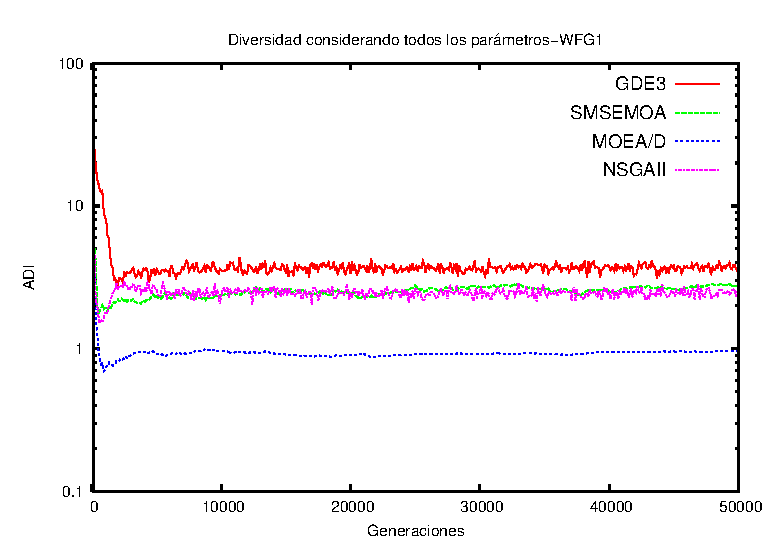
\includegraphics[width=0.5\textwidth]{Figures_Chapter1/Average_FullParamsStateArt.eps} 
    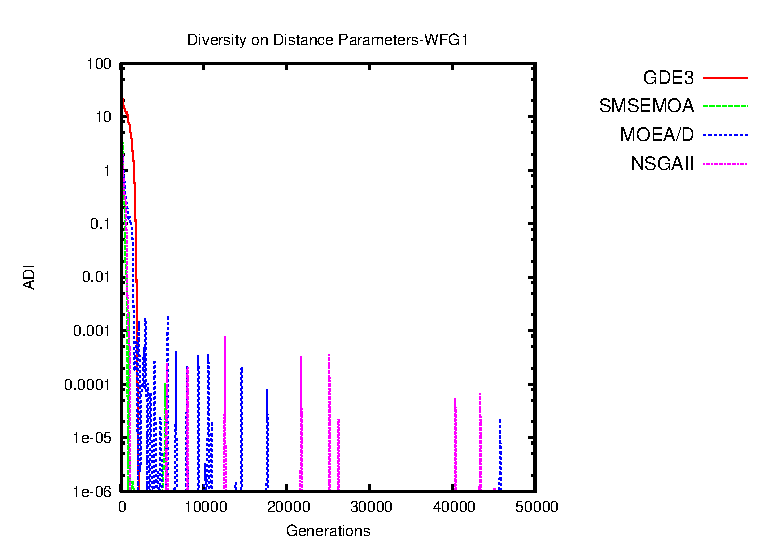
\includegraphics[width=0.5\textwidth]{Figures_Chapter1/Average_DistanceParamsStateArt.eps}  \\
    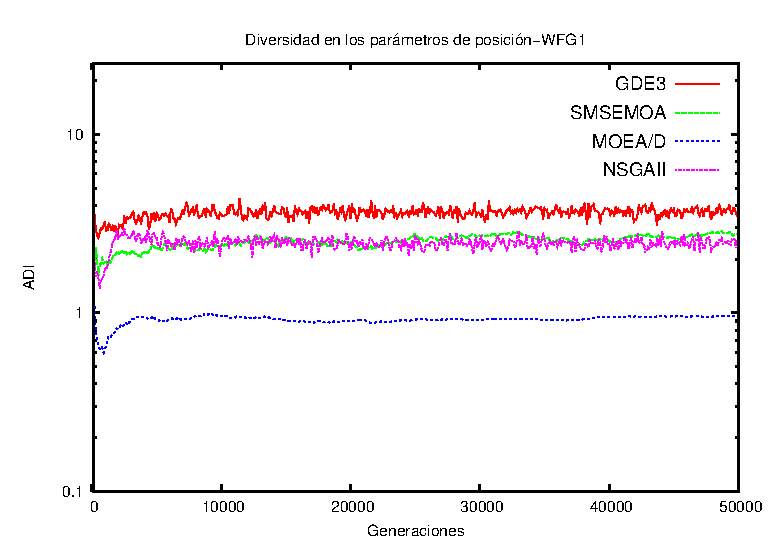
\includegraphics[width=0.5\textwidth]{Figures_Chapter1/Average_PositionParamsStateArt.eps}  
\end{tabular}
\caption{Evolución ADI del estado-del-arte en la instancia WFG1 (escala logarítmica).}
%\caption{Evolution of the DCN for state of art considered (WFG1 instance) in logarithmic scale.}
\label{fig:Average_StateArtDiversityDistanceParameters}
\end{figure}

\begin{figure}[H]
\centering
    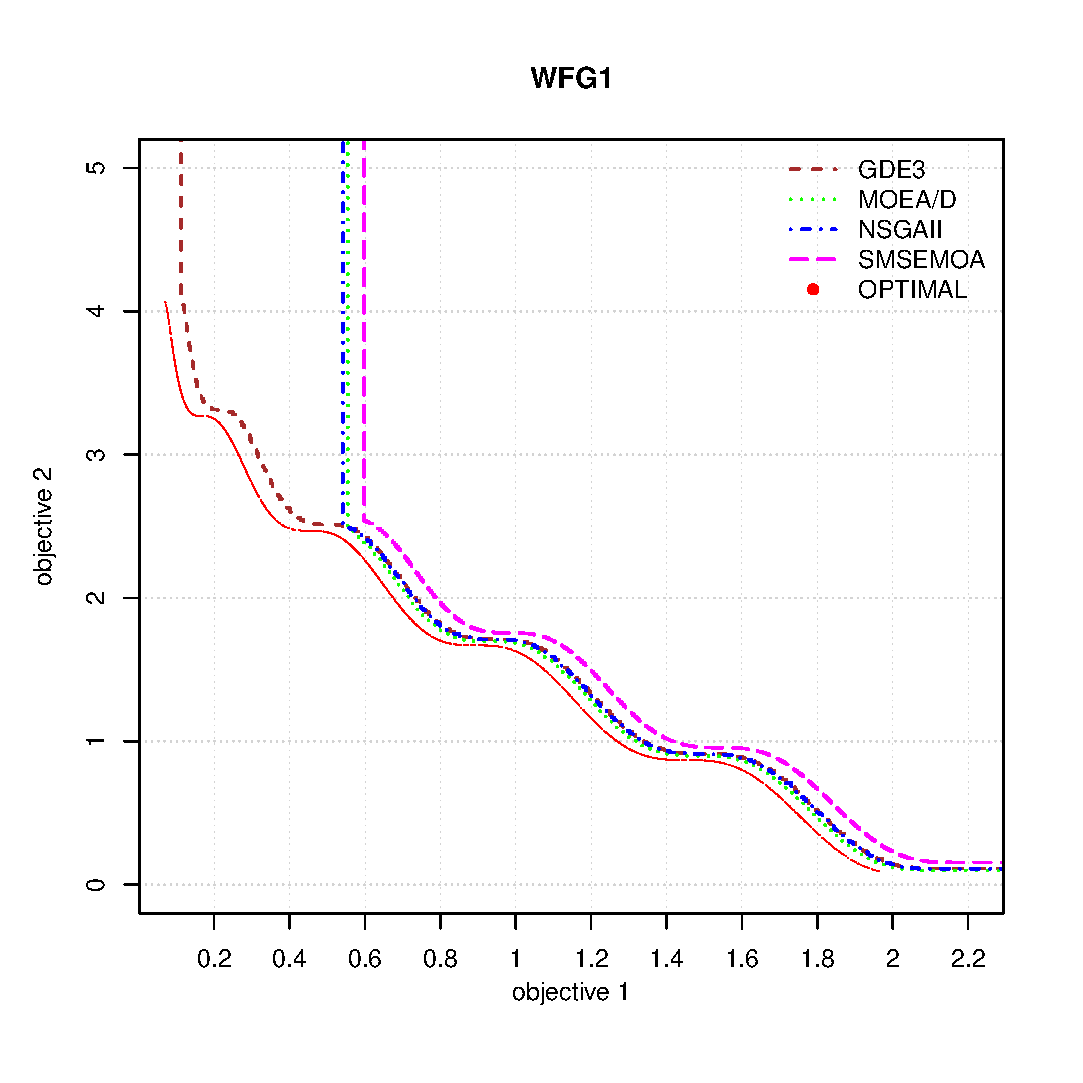
\includegraphics[width=0.5\textwidth]{Figures_Chapter1/WFG1.eps}  
\caption{Superficies de curbimiento logradas al 50\% en el problema de pruena WFG1.}
\label{fig:Superficie_WFG1}
\end{figure}




%In fact, after about 5,000 generations most of the current approaches have completely lost the diversity in the distance parameters subset. Thus, when taking into account this subspace, it can be considered that all these approaches converge prematurely, meaning that in long-term executions, most of the generations are wasted by these algorithms. 
%In this paper we prove that considering diversity in variable space can offer better approximations of the Pareto fronts and that some difficulties related to premature convergence can be avoided. In order to properly prove these facts, the hyper-volume metric and adequate statistical tests are reported. Additionally, attainment surfaces are taken into account. Some of the most difficult problems such as the WFG8 are readily solved by our proposal. However, some difficulties appear in the WFG6 and WFG9. The reasons of these drawbacks are related to the fact that the mating restrictions considered in this paper, provokes a bias to create more individuals in the regions placed near the corners of the search space. Thus, when some of these regions have some promising, but non-optimal solutions, convergence to such regions might appear.



\section{Organización de la tesis}

El presente documento consta de siete capítulos donde se describe el trabajo realizado, los resultados obtenidos y las conclusiones.
%
A continuación, se explica de forma breve el contenido de los siguientes capítulos.
%

En el \textbf{Capítulo \ref{Chapter2}}, se definen formalmente los conceptos en el ámbito multi-objetivo, se presenta una recopilación de los MOEAs más importantes en la literatura.
%
Además se describen los algoritmos utilizados como el estado-del-arte, donde es elegido al menos uno de cada categoría de los MOEAs: basado en dominancia, basado en descomposición y basado en indicadores.
%
También se hace una recopilación de los problemas de referencia ampliamente utilizados (ZDT, DTLZ, WFG y UF).
%
Al final de este capítulo se describen algunas de las técnicas para medir el desempeño de las soluciones generadas por un MOEA.
%

El \textbf{Capítulo \ref{Chapter3}} presenta una revisión de los MOEAs que consideran la diversidad en el espacio de la variables como parte del proceso de búsqueda.
%
Específicamente, es propuesto el VSD-MOEA siendo el primer algoritmo de su tipo, ya que considera la diversidad en el espacio objetivo y en el espacio de las variables simultáneamente, además es basado en dominancia.
%

En el \textbf{Capítulo \ref{Chapter4}} se realiza una revisión de la literatura sobre algunas estrategias para mejorar el mecanismo de emparejamiento y/o remplazo, de igual forma se revisan algunos de los métodos generadores de pesos y se presenta detalladamente el método generador que es implementado en este trabajo.
%
Posteriormente, se presentan tres propuestas algorítmicas basadas en descomposición, el primero mantiene la diversidad de las variables de forma implícita y los otros dos de forma explícita.
%

En el \textbf{Capítulo \ref{Chapter5}} es presentado un análisis del operador genético de Cruce Binario Simulado (SBX) y de los operadores de evolución diferencial en esquemas de diversidad a largo plazo.

La validación experimental es llevada a cabo en el capítulo \textbf{Capítulo \ref{Chapter6}}, donde se realizan pruebas estadísticas, se muestran superficies de cubrimiento logradas y se hacen un análisis de escalabilidad en las variables con la propuesta inicial de dominancia.


%
Finalmente, en el \textbf{Capítulo \ref{Chapter7}} se presentan las conclusiones en base a los resultados obtenidos en este documento, además se discuten los trabajos futuros a desarrollar como resultado de esta investigación.

% Chapter 1

\chapter{Optimización Multi-objetivo} % Main chapter title

\label{Chapter2} % For referencing the chapter elsewhere, use \ref{Chapter1} 

%----------------------------------------------------------------------------------------

% Define some commands to keep the formatting separated from the content 
%\newcommand{\keyword}[1]{\textbf{#1}}
%\newcommand{\tabhead}[1]{\textbf{#1}}
%\newcommand{\code}[1]{\texttt{#1}}
%\newcommand{\file}[1]{\texttt{\bfseries#1}}
%\newcommand{\option}[1]{\texttt{\itshape#1}}

%----------------------------------------------------------------------------------------
\section{Conceptos}
Un problema de optimización multi-objetivo (MOP) representa un conjunto de funciones objetivo las cuales deben minimizarse o maximizarse simultánemante, estas funciones usualmente se encuentran en conflicto.
%

Un problema de optimización multi-objetivo se formula como se indica en la ecuación (\ref{eqn:MOOP}).

\begin{equation}
\begin{split}
Minimizar/Maximizar \quad &f_m(\vec{x}) \quad m=1,2, ..M \\
sujeto\quad a \quad &g_j(\vec{x}) \geq 0 \quad j = 1,2, ... J\\
&h_k(\vec{x}) = 0, \quad k=1,2, ..., K\\
&x_i^{(L)} \leq x_i \leq x_i^{(U)} \quad i = 1,2, ..., n
\end{split}
\label{eqn:MOOP}
\end{equation}

Donde solución $\vec{x}$ es un vector de $n$ variables de decisión $x = (x_1, x_2, ..., x_n)^T$, la última desigualdad corresponde a los límites de las variables, restringiendo cada variable de decisión $x_i$ por su límite inferior $x_i^{(L)}$ y su límite superior $x_i^{(U)}$, conformando así el espacio de las variables de decisión. 
%
En relación con el problema existen $\textbf{J}$ desigualdades y $\textbf{K}$ restricciones.
%
Los términos $g_j(\vec{x})$ y $h_j(\vec{x})$ son conocidos como las funciones de restricción.
%
Una solución $\vec{x}$ que no satisface todas las (\textbf{J+K}) restricciones en los límites de las variables es conocida como una \textit{Solución no factible}. 
%
Si cualquier solución $\vec{x}$ satisface todas las restricciones y los límites, es conocida como una \textit{Solución factible}.
%
El conjunto de todas las soluciones factibles es conocida como la \textit{región factible} $\Omega$.\\
A diferencia de un sólo objetivo, en optimización multi-objetivo un vector de variables que corresponden al espacio de decisión $n$-dimensional es mapeado a un punto en el espacio $m$-dimensional conocido como \textit{espacio objetivo} $Z$.
%----------------------------------
\subsection{Dominancia}

\subsubsection*{Concepto de Dominancia}
Se dice que una solución $\vec{x}$ domina a otra solución $\vec{y}$ matemáticamente $\vec{x} \preceq \vec{y}$, si las dos condiciones son cumplidas:
\begin{itemize}
\item La solución $\vec{x}$ no es peor que la solución $\vec{y}$ en todos los objetivos.\\
$\forall m \in \{ 1, 2, ..., M \}: f_m(x_i) \leq f_m(y_i)$
\item La solución $\vec{x}$ es estrictamente mejor que la solución $\vec{y}$ en al menos un objetivo.\\
$\exists m \in \{ 1, 2, ..., M \}: f_m(x_i) < f_m(y_i)$
\end{itemize}
%---------------------------
\subsubsection*{Propiedades de dominancia}
Se derivan las siguientes propiedades, considerando las soluciones $\vec{p}$, $\vec{q}$ y $\vec{r}$ entonces:
\begin{itemize}
\item Reflexiva: La relación de dominancia no es reflexiva, dado que la solución no se domina a si misma.
\item Simétrica: La relación de dominancia es no simétrica, ya que si  $ \vec{p} \preceq \vec{q}$  no implica que $\vec{q} \preceq \vec{p}$, entonces la relación de dominancia es asimétrica.
\item Anti-simétrica: Dado que la relación de dominancia es no simétrica, esta no puede ser anti-simétrica.
\item Transitiva: La relación de dominancia es transitiva. Esto se debe a que si $\vec{p} \preceq \vec{q}$ y $\vec{q} \preceq \vec{r}$, entonces $\vec{p} \preceq \vec{r}$.
\end{itemize}
%%-------------
\subsubsection*{Conjunto no dominado}
Dado un conjunto de soluciones $ \mathbf{P}$, el conjunto de soluciones no dominadas $\mathbf{P'}$ son aquellas que no son dominadas por cualquier otro miembro del conjunto $ \mathbf{P}$.
Así si $\mathbf{P}$ es considerado como el espacio de búsqueda ($\mathbf{P} = \Omega$) entonces el conjunto no dominado $\mathbf{P'}$ es el conjunto óptimo de Pareto.
%%---------------
\subsubsection*{Dominancia fuerte}
Se define como dominancia fuerte si una solución $\vec{x}$ es estrictamente mejor que otra solución $\vec{y}$ en todos los objetivos, definido matemáticamente como $ \vec{x} \prec \vec{y} $.

%%-------------
\subsubsection*{Dominancia débil}
Entre un conjunto de soluciones $\mathbf{P}$, el conjunto de soluciones débilmente dominadas $\mathbf{P'}$ son consideradas como las soluciones que no son fuertemente dominadas por cualquier otro miembro del conjunto $\mathbf{P}$. Esto es una soluci\'on $\vec{x}$ domina d\'ebilmente a otra soluci\'on $\vec{y}$ denotado por $\vec{x} \preceq \vec{y} $,  si y s\'olo si $\forall i \in \{1,...,m\}$, $f_i(\vec{x}) \leq f_i(\vec{y})$.
%%-------------------------
\subsubsection*{Solución óptima de Pareto}
Una solución $\vec{x}^*$ es considerada como óptimo de Pareto si no existe otra solución factible $\vec{y}$ que dado un criterio mejore la calidad del resultado obtenido por $\vec{x}^*$.\\
$\vec{x}^* \in F  \iff  \nexists \vec{y} \in F \rightarrow \vec{y} \preceq \vec{x}^*  $ 
%%-------------
\subsubsection*{Conjunto óptimo de Pareto}
Dada la región factible $\Omega$ de un MOP, el conjunto óptimo de Pareto $\mathbf{P^*}$ se define como:
\begin{equation*}
\mathbf{P^*} = \{ \vec{x}^* \in \Omega  \}
\end{equation*}
%%-------------
\subsubsection*{Frente de Pareto}
Sea $\mathbf{P^*}$ el conjunto óptimo de Pareto, el frente de Pareto $\mathbf{PF^*}$ corresponde a todas las imágenes del conjunto óptimo de Pareto.
%%--------------
\subsubsection*{Vector objetivo Ideal}
El vector objetivo ideal $\vec{z}^*$ es la solución construida en base al punto óptimo de cada función objetivo. 
%
Así si la solución mínima para cada función objetivo es el conjunto de vectores de decisión $\vec{x}^{*(m)}$ con su correspondiente imágen ${f_m^*}$, entonces  el vector ideal se define como:
\begin{equation*}
%\vec{z}^* = \vec{f}^* = (f_1^*, f_2^*, ..., f_M^*)^T
z_i^* = min_{\vec{x}} f_i(\vec{x})
\end{equation*}
El vector objetivo ideal define los límites inferiores\footnote{En el caso de maximizción en todos los objetivos se define de la forma $z_i^* = max_{\vec{x}} f_i(\vec{x})$ .} para todos los objetivos, es decir que en el espacio de búsqueda factible $\Omega$ existe al menos una solución en cada objetivo que corresponde con un componente del vector ideal.
\subsubsection*{Vector objetivo Utópico}
Un vector objetivo utópico $\vec{z}^{**}$ tiene definido cada uno de sus componentes marginalmente menor en el espacio objetivo que el correspondiente vector ideal, donde cada $i$-ésimo componente está definido de la forma:
\begin{equation}
z_i^{**} = z_i^* - \epsilon_i
\end{equation}
donde $\epsilon_i > 0 \quad \forall i \in {1, 2, ..., M}$.
\\
El vector utópico se utiliza como punto de referencia en los algoritmos donde existe una condición la cual una solución debe ser estrictamente mejor que otra solución.
%%------------------------------
\subsubsection*{Vector Objetivo Nadir}
El vector nadir representa el límite superior de cada objetivo en el conjunto óptimo de Pareto  y no en todo el espacio de búsqueda. 
%
Este vector es construido utilizando los peores valores de $\mathbf{PF}^*$, cada $i$-ésimo componente es definido como:
\begin{equation*}
z_i^{nad} = max_{\vec{x} \in P^*} f_i(\vec{x})
\end{equation*}
%
El vector objetivo nadir puede representar una solución existente o no existente dependiendo de la forma que posea el conjunto óptimo de Pareto.

\begin{figure}[h]
\centering
\scriptsize
%\includegraphics[width=6cm, height=6cm]
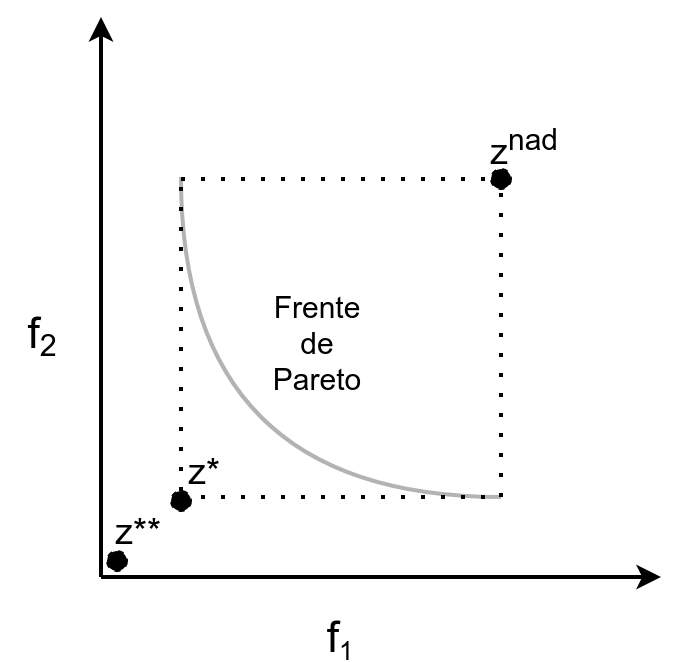
\includegraphics[scale=0.3]
{Figures_Chapter2/Componentes_Multiobjetivo.png}
\decoRule
\caption{Ubicación de los vectores ideal, utópico y nadir en el caso de dos objetivos.}
\label{fig:Componentes_Multiobjetivo}
\end{figure}
%----------------------------------
\section{Algoritmos Evolutivos Multi-objetivo}

\subsection{Métodos Clásicos}

Los métodos clásicos desarrollados para resolver problemas de optimización multi-objetivo han sido clasificados por varios autores, entre ellos Cohon (1985) quien propuso la clasificación de la siguiente forma:
\begin{itemize}
\item \textbf{Métodos generadores}. En estos métodos se generan pocas soluciones no dominadas por el tomador de decisiones (decision-maker) quien toma una solución no dominada según un criterio a fin. Además no se utiliza un conocimiento a priori para cada objetivo.
\item \textbf{Métodos basados en preferencia}. En este tipo de métodos se indica una preferencia especial en cada objetivo. 
\end{itemize}
Posteriormente Hwang y Masud (1979) y posteriormente Miettien (1999), clasificaron los métodos en las siguientes categorías:
\begin{itemize}
\item \textbf{Métodos no preferenciales}. Este tipo de métodos no utilizan información para asignar una preferencia a objetivos específicos, además no utilizan estrategias para encontrar múltiples soluciones óptimas de Pareto.
\item \textbf{Métodos posteriori}. En esta categoría se utiliza información preferencial para encontrar múltiples soluciones en el frente de Pareto, posteriormente el tomador de decisiones mediante un criterio a fin decide las soluciones a utilizar (búsqueda $\rightarrow$ decisión).
\item \textbf{Métodos a priori}. En esta categoría se utiliza información preferencial transformando el problema en mono-objetivo o múltiples problemas mono-objetivo, normalmente se realiza la búsqueda de una solución óptima de Pareto (decisión $\rightarrow$ búsqueda).
\item \textbf{Métodos interactivos}. Este tipo de métodos utilizan información preferencial donde progresivamente durante el proceso se ve involucrado el tomador de decisiones para obtener soluciones aproximadas al frente de Pareto (decisión $\leftrightarrow$ búsqueda). 
\end{itemize}
	
\subsubsection{Método de sumas ponderadas}
El método de sumas ponderadas transforma un problema multi-objetivo en un problema mono-objetivo, por medio de la pre-multiplicación de cada objetivo con un peso el cual es definido por el tomador de decisiones.  El peso asignado a cada objetivo depende de la importancia que se desea dar a cada objetivo en el contexto del problema. Asignar un vector de pesos apropiado depende también de la escala en cada función objetivo, por lo que es necesario normalizar los objetivos para que cada uno tenga la misma importancia.

\begin{equation} \label{eqn:Suma_Ponderada}
\begin{matrix}
%\begin{eqnarray} \label{eqn:Suma_Ponderada}
Minimizar         & F(\vec{x})= \sum_{m=1}^M w_m f_m(\vec{x}), &  \\
sujeto\quad a & g_j(\vec{x}) \geq 0,                          & j=1, 2, ..., J;\\
                 & h_k(\vec{x}) = 0,                             & k=1,2, ..., K; \\
                 & x_i^{(L)} \leq x_i \leq x_i^{(U)}                & i=1, 2, ..., n.
%\end{eqnarray}
\end{matrix}
\end{equation}
En la ecuación $w_m$ ($\in [0,1]$) se refiere al peso de la $m$-ésima función objetivo, en el problema definido en la ecuación \ref{eqn:Suma_Ponderada}  cada componente que corresponde al vector de pesos, el cual es invariante al ser multiplicado por una constante, usualmente se escogen los pesos de la forma
%\begin{equation*}
$\sum_{m=1}^M w_m = 1$.
%\end{equation*}
\newtheorem{Classic}{Definition}

\begin{Classic}
Una solución al problema de la ecuación (\ref{eqn:Suma_Ponderada}) es óptimo de Pareto, sólo si cada componente del vector de pesos es positivo.
\end{Classic}

\begin{Classic}
\textit{Si  $\vec{x}^*$ es una solución óptima de Pareto en un problema de optimización multi-objetivo convexo, entonces existe un vector de pesos positivos diferentes de cero $\vec{w}$ tal que $\vec{x}^*$ es la solución proporcionada por la ecuación (\ref{eqn:Suma_Ponderada})}
\end{Classic}
\subsubsection*{Ventajas}
Es una de las formas más sencillas para resolver un MOP. El concepto es fácil de utilizar. Para problemas que tienen un frente óptimo de Pareto con forma convexa, este método garantiza encontrar las soluciones en el conjunto óptimo de Pareto.
\subsubsection*{Desventajas}
Es difícil asignar los pesos que puedan mapear soluciones distribuidas uniformemente en el frente óptimo de Pareto.
Distintos vectores de pesos no necesariamente llevan a diferentes soluciones óptimas de Pareto.
\subsubsection*{Dificultades con problemas no convexos}
El método de sumas ponderadas no puede encontrar ciertas soluciones óptimas de Pareto en el caso de frentes no convexos.

%------------------------------------------
\subsubsection{Método de restricción}
Se reformula el problema de optimización multi-objetivo manteniendo un objetivo y restringiendo el resto de objetivos  con valores especificados por el usuario.

\begin{equation} \label{eqn:Metodo_Restricciones}
\begin{matrix}
%\begin{eqnarray} \label{eqn:Suma_Ponderada}
Minimizar         & f_{\mu}(\vec{x}), &  \\
sujeto \quad a & f_m(\vec{x}) \leq \epsilon_m					& m=1, 2, ..., M \quad and \quad m \neq \mu\\
				 & g_j(\vec{x}) \geq 0,                          & j=1, 2, ..., J;\\
                 & h_k(\vec{x}) = 0,                             & k=1,2, ..., K; \\
                 & x_i^{(L)} \leq x_i \leq x_i^{(U)}                & i=1, 2, ..., n.
%\end{eqnarray}
\end{matrix}
\end{equation}
El parámetro $\epsilon_m$ representa un límite superior del valor de $f_m$.
\begin{Classic}
La solución única en un problema de restricciones con $\vec{\epsilon}$ establecido en la ecuación (\ref{eqn:Metodo_Restricciones}) es óptimo de Pareto para cualquier límite superior definido por el vector ($\epsilon_1, ..., \epsilon_{\mu-1}, \epsilon_{\mu+1}, ..., \epsilon_{M})^T$.
\end{Classic}
\subsubsection*{Ventajas}
Diferentes soluciones óptimas de Pareto pueden ser encontradas utilizando distintos valores de $\epsilon_m$. El mismo método puede ser utilizado en cualquier problema de optimización multi-objetivo incluyendo los que poseen frentes de Pareto convexos o no convexos.
\subsubsection*{Desventajas}
La ecuación (\ref{eqn:Metodo_Restricciones}) depende totalmente del vector de restricciones $\vec{\epsilon}$ establecido, el cual debe estar en el dominio comprendido por el espacio objetivo. Al aumentar el número de objetivos se necesita mas información por parte del tomador de decisiones ya que existen más elementos en el vector $\vec{\mathbf{\epsilon}}$.
%-----------------------------------------------------
\subsubsection{Métodos con métricas ponderadas}
En lugar de utilizar la suma de pesos ponderados en el espacio objetivo, se utilizan otras estrategias las cuales convierten problemas multi-objetivos a mono-objetivos.
%
Por lo regular se utilizan métricas de distancia $l_p$ y $l_{\inf}$. 
%
En el caso de pesos no negativos la métrica ponderada $l_p$ establece que si se tiene una solución $\vec{x}$ y un vector ideal $\vec{z}^*$ es posible modelar en un problema de minimización como se indica en la ecuación ~\ref{eqn:Metodo_Metricas_Ponderadas}.

\begin{equation} \label{eqn:Metodo_Metricas_Ponderadas}
\begin{matrix}
Minimizar         & l_p(\vec{x}) = \left (   \sum_{m=1}^M W_m |f_m( \vec{x} ) - z_m^* |^p \right)  ^{1/p}, 							&  \\
sujeto \quad a 				 & g_j(\vec{x}) \geq 0,                          & j=1, 2, ..., J;\\
                 & h_k(\vec{x}) = 0,                             & k=1,2, ..., K; \\
                 & x_i^{(L)} \leq x_i \leq x_i^{(U)}                & i=1, 2, ..., n.
\end{matrix}
\end{equation}
El parámetro $p$ puede tomar cualquier valor entre $[1, \infty]$.
%
Cuando se asigna el valor $p=1$ el problema es equivalente al método de sumas ponderadas. 
%
Por otra parte si se asigna $p=2$ se realiza el cálculo de la distancia Euclídea la cual busca minimizar la distancia entre cualquier punto y el punto ideal.
%
En el caso en particular que $p \rightarrow \infty$ el problema se transforma en minimizar la mayor desviación descrita por $|f_x(\vec{x}) - z_m^*|$. Este último caso se conoce como el problema de \textit{Tchebycheff ponderado}:
\begin{equation} \label{eqn:Metodo_Tchebycheff_Ponderado}
\begin{matrix}
Minimizar         & l_{ \infty }(\mathbf{x}) = \left ( max_{m=1}^M w_m| f_x(\vec{x}) - z^*_m|   \right), 							&  \\
sujeto \quad a 				 & g_j(\vec{x}) \geq 0,                          & j=1, 2, ..., J;\\
                 & h_k(\vec{x}) = 0,                             & k=1,2, ..., K; \\
                 & x_i^{(L)} \leq x_i \leq x_i^{(U)}                & i=1, 2, ..., n.
\end{matrix}
\end{equation}
\subsubsection*{Ventajas}
La métrica de Tchebycheff ponderada garantiza encontrar cualquier solución óptima de Pareto (incluso en problemas no convexos), siempre y cuando $\vec{z}^*$ sea un el vector utópico.

\subsubsection*{Desventajas}
La magnitud de los objetivos influye en los resultados, por lo que es necesario normalizar los objetivos, esto requiere el conocimiento del mínimo y del máximo de cada objetivo. En este método es requerida la solución ideal $\vec{z}^*$. Por lo que todos los $M$ objetivos son necesarios para ser optimizados independientemente antes de optimizar la métrica $l_p$.

\subsection{Métodos Iniciales}


\subsubsection{Algoritmo Genético basado en Evaluación de Vectores - VEGA}
%\subsubsection{Vector Evaluated Genetic Algorithm (VEGA)}
Una de las primeras implementaciones de un algoritmo evolutivo multi-objetivo fue sugerido por  \citeauthor{Joel:VEGA} en \citeyear{Joel:VEGA}, este algoritmo consiste que en dado un problema multi-objetivo conformado por $M$ objetivos y una población de tamaño $N$, se realiza la divisi\'on de la población en $M$ subpoblaciones iguales de forma aleatoria, a cada subpoblación se le asigna una aptitud basada en su respectiva función objetivo. Entonces cada una de las $M$ funciones objetivo es utilizada para evaluar algunos miembros de la población.
\begin{algorithm}[H]
%%\algsetup{linenosize=\tiny}
  \scriptsize
	\caption{Algoritmo Genético basado en Evaluación de Vectores - VEGA} 
	\begin{algorithmic}[1]
    \STATE $N$: el n\'umero de individuos, $M$: el n\'umero de objetivos
    \STATE $q=M/N$
    \FOR{$i=1$ hasta $M$} 
       \FOR{ cada solución  $j=1+(i-1)*q$ hasta $j=i*q$ }
    	 \STATE Asignar una aptitud $F(X^{(j)})=F_i(X^{(j)})$
       \ENDFOR
    \STATE Realizar la selección apropiada en las $q$ soluciones para crear un conjunto de emparejamiento $\mathbf{P_i}$.
    \ENDFOR
    \STATE Combinar el conjunto de emparejamiento $\mathbf{P} = \cup_{i=1}^M \mathbf{P_i}$, implementar los operadores de cruce y mutación en $\mathbf{P}$ para generar una nueva población.
    \end{algorithmic}
    \label{alg1}
\end{algorithm}
Este algoritmo genera mejores soluciones en problemas donde no existe un grado de dependencia.
%
Schaffer implementa el operador de cruce entre dos individuos en toda la población, con el objetivo de que al cruzar dos buenas soluciones que corresponden a distintos objetivos, se puedan encontrar buenas soluciones entre los dos objetivos.
%
La mutación polinomial se aplica a cada individuo como normalmente se realiza en algoritmos multi-objetivo.
\subsubsection*{Ventajas}
La principal ventaja del algoritmo VEGA es su facilidad de implementación ya que la idea es simple.
%
Este algoritmo tiene una tendencia para encontrar soluciones cercanas a las mejores soluciones individualmente en cada función objetivo. 
%
En problemas separables, donde el espacio solución está comprendido por las mejores soluciones independientemente en cada función objetivo se considera como una estrategia ideal.

\subsubsection*{Desventajas}
En este algoritmo cada solución es evaluada sólo con una función objetivo, entonces no se analiza el resultado de las soluciones en las otras $M-1$ funciones objetivo, lo cual es importante en el contexto multi-objetivo, además el operador de cruce entre las mejores soluciones individuales puede no generar soluciones diversas.

\subsubsection{Algoritmo Genético de Múltiples Objetivos - MOGA}
%\subsubsection{Multiple Objective Genetic Algorithm (MOGA)}

Este algoritmo fue propuesto por los autores \citeauthor{Joel:MOGA} en \citeyear{Joel:MOGA}, el cual utiliza la relación de dominancia para clasificar cada solución de la población del algoritmo genético.
%
En la primera sugerencia los autores enfatizaron el hecho de establecer estrategias enfocadas a las soluciones no dominadas y simultáneamente mantener diversidad de las mismas. 
%
En este algoritmo se le asigna un rango a cada solución, este rango se basa en el número de individuos dominados dentro de la población, entonces para la solución $i$ el rango es asignado como la suma de la unidad y el número de soluciones $n_i$ que dominan a la solución $i$.
\begin{equation}
r_i  = 1 + n_i
\end{equation}
Las soluciones no dominadas tienen asignado el rango igual a uno, indicando que no existe otra solución que sea mejor en todos los objetivos.
%
En cualquier población debe existir al menos una solución con rango igual a uno y el máximo rango de cualquier miembro en la población no puede ser mayor al tamaño de la población $N$, además es posible que existan rangos no asignados en la población.
%
Una vez asignados los rangos se asigna una aptitud a cada individuo en base a su rango.
%
El proceso consiste en primero ordenar las soluciones en base a su rango en forma ascendente.
%
Entonces una aptitud es asignada a cada solución utilizando una función lineal. 
%
Posteriormente, son promediadas las aptitudes que corresponden a las soluciones de cada rango, resultando así la aptitud efectiva en cada individuo.
%
Este mecanismo permite que las soluciones no dominadas sean preferidas en la población.  

\begin{algorithm}[H]
%%\algsetup{linenosize=\tiny}
  \scriptsize
	\caption{Procedimiento para la asignación de Aptitud - MOGA} 
	\begin{algorithmic}[1]
    \STATE $\sigma_{share}$: distancia mínima para cada nicho, $M$: el número de objetivos
    \STATE $\mu (j) = 0$ $\forall j \in N$
    \FOR{$i=1$ hasta $N$} 
    \STATE Calcular el número de soluciones ($n_i$) que dominan a la solución $i$ 
	\STATE $r_i = 1+ n_i$
    \STATE $\mu(r_i)=\mu(r_i) + 1$
    \ENDFOR
\FOR{Para cada solución en el rango $r$}
    \STATE $F_i = N \sum_{k=1}^{r_i - 1} \mu(k) - 0.5(\mu( r_i)-1)$
    \STATE $F_j^, = \frac{F_j}{nc_j} $
    \STATE $F_i^, \leftarrow  \frac{F_j \mu(r)}{  \sum_{k=1}^{\mu(r)} F_k^,  } F_j^,$
 \ENDFOR
    \end{algorithmic}
    \label{alg1}
\end{algorithm}


%\subsubsection{%Niched-Pareto Genetic Algorithm (NPGA)}
\subsubsection{Algoritmo Genético basado en Nichos de Pareto - NPGA}
El algoritmo NPGA propuesto por \citeauthor{Joel:NPGA} en \citeyear{Joel:NPGA} implementa la selección basada en el torneo binario en lugar de la selección proporcional, a diferencia del VEGA, NSGA y otros algoritmos multi-objetivo, esto se debe a que en base a varios estudios ( Goldberg and Deb, 1991) se ha demostrado que la selección basada en el torneo binario proporciona mejores propiedades relacionadas con la convergencia en comparación a la selección proporcional.
%
Sin embargo existe una dificultad al implementar simultáneamente cualquier selección no proporcional  y el enfoque de función compartida (\textit{shared function}), ya que el enfoque de funciones compartidas ubica soluciones en un nicho el cual es proporcional a la aptitud promedio del nicho.\\
%
Este algoritmo implementa una estrategia de nichos la cual es actualizada dinámicamente,  durante la selección basada en torneo binario, se escogen dos soluciones $i,j$ en forma aleatoria de la población padre $\mathbf{P}$ .
%
Estas soluciones son comparadas seleccionando una subpoblación $\mathbf{T}$ de tamaño $t_{dom}$ de la población. Posteriormente cada solución $i$ y $ j$ es comparada con cada solución de la subpoblación basados en el criterio de la dominancia.
%
De las dos soluciones, si una solución domina a todas las soluciones de la subpoblación esta solución es elegida.
%
Si cualquiera de las dos soluciones $i$ y $j$ son dominadas por al menos una solución en la subpoblación o las dos no son dominadas por cualquier solución en la subpoblación las dos soluciones se verifican con la población de hijos $\mathbf{Q}$ (parcialmente llena), posteriormente se implementa un conteo de nichos, que consiste en contar el número de soluciones más cercanas a una solución de referencia.
%
La solución con el menor conteo de nichos gana en el torneo.

\begin{algorithm}[H]
%%\algsetup{linenosize=\tiny}
  \scriptsize
	\caption{NPGA - Procedimiento principal} 
	\begin{algorithmic}[1]
    \WHILE{ $i \leq N$}
    \STATE Implementar la selección por torneo binario y encontrar el primer padre $p_1 = NPGA -Torneo binario(i, i+1, \mathbf{Q})$
    \STATE $i=i+2$ 
    \STATE Encontrar el segundo padre $p_2 = NPGA -Torneo binario(i, i+1, \mathbf{Q})$
    \STATE Implementar la cruza entre las soluciones padres $p_1$ y $p_2$ y crear las soluciones hijos $c_1$ y $c_2$ 
    \STATE Actualizar las soluciones hijo $Q = Q \cup \{ c_1, c_2 \}$
    \STATE $i=i+1$ 
    \ENDWHILE
    \end{algorithmic}
    \label{alg1}
\end{algorithm}

\begin{algorithm}[H]
%%\algsetup{linenosize=\tiny}
  \scriptsize
	\caption{NPGA - Torneo binario} 
	\begin{algorithmic}[1]
   \STATE Obtener una subpoblación $\mathbf{T_{ij}}$ de tamaño $t_{dom}$ de la población padre $\mathbf{P}$ 
   \STATE Calcular $\alpha_i$ como el número de soluciones en $\mathbf{T_{ij}}$ que domina a $i$  
     \STATE Calcular $\alpha_j$ como el número de soluciones en $\mathbf{T_{ij}}$ que domina a $j$
     \IF{ $\alpha_i = 0$ y $\alpha_j > 0$   }
        \STATE $i$ es el ganador y el proceso de selección está completo.
      \ELSIF{ $\alpha_i > 0$ y $\alpha_j = 0$}
      	 \STATE $j$ es el ganador y el proceso de selección está completo.
      \ELSE
      	 \IF{ $|Q| < 2 $ }
            \STATE $i$ o $j$ es escogido con probabilidad de $0.5$ el proceso está completo.
          \ENDIF
          \STATE En caso de no cumplirse ninguna condición se realiza un conteo con nichos $nc_i$ y $nc_j$ ubicando $i$ y $j$ en la población hijo $\mathbf{Q}$ de forma independiente. El parámetro de nichos $\sigma_{share}$ .
          \STATE $d_{ik} = \sqrt{ \sum_{m=1}^M  \left ( \frac{ f_m^{(i)} -f_m^{(k)}  }{ f_m^{max} - f_m^{min} }  \right )}$ 
          \STATE $nc_{i}$ es calculado como el número de soluciones $k$ en $\mathbf{Q}$ con una distancia $d_{ik}$ desde $i$ menor a $\sigma_{share}$ 
          \IF{ $nc_i \leq nc_j$}
             \STATE $i$ es el ganador.
            \ELSE
               \STATE $j$ es el ganador.
          \ENDIF
     \ENDIF
    \end{algorithmic}
    \label{alg1}
\end{algorithm}



\subsubsection*{Ventajas}
Una de las principales ventajas del NPGA es que no se necesita una asignación explícita de la aptitud a diferencia de los algoritmos VEGA, NSGA y MOGA.
Este es el primer algoritmo evolutivo multi-objetivo el cual utiliza el operador de selección por torneo.
El NPGA realiza un muestreo de la población para generar una subpoblación, si la subpoblación es de un tamaño pequeño puede resultar eficiente resolviendo problemas con muchos objetivos.
\subsubsection*{Desventajas}
Requiere la configuración de dos parámetros: $\sigma_{share}$ y $t_{dom}$. El parámetro $\sigma_{share}$ tiene un efecto importante en NPGA, ya que realiza el conteo de los individuos en el nicho, que a diferencia del NSGA no se toma el valor de la distancia explícitamente.

\subsection{Métodos Actuales}
En las últimas décadas el campo de los algoritmos evolutivos multi-objetivo han ganado popularidad, fomentando un crecimiento considerable de los mismos.  
%
En la literatura se  clasifican los algoritmos evolutivos multi-objetivo basados en dominancia, basados en descomposición y/o basados en indicadores (\cite{Joel:ShortSurveyStateArt}). 
%
Actualmente no existe un algoritmo el cual sea considerado superior entre las distintas clasificaciones.
%
\subsubsection{Métodos basados en dominancia}
Este tipo de algoritmos evolutivos multi-objetivo están basados en la relación de dominancia de Pareto.%, los cuales se utilizan para el diseño de los algoritmos. 
%
Particularmente se implementa un conteo en base a la relación de dominancia para asignar un valor de aptitud.
%
Debido a que la relación de dominancia no promueve la diversidad en el espacio objetivo, se implementan técnicas explícitas como la implementación de nichos y/o otros mecanismos de agrupamiento.
%
Bajo estos dos principios es posible obtener soluciones cercanas al frente de Pareto y propiamente distribuidas.
%
Un algoritmo considerado popular y que pertenece a esta clasificación es el Algoritmo Genético basado en Ordenación de No dominados II (NSGA-II) propuesto por \cite{Joel:NSGAII}. Este algoritmo implementa un operador especial para la selección de padres e incorpora elitismo en la fase de reemplazamiento. 
%
El operador de selección de padres se basa en dos mecanismos: Ordenación eficiente de no dominados (\textit{fast-non-dominated-sort}) y amontonamiento de soluciones (\textit{crowding}).
%
El primero se basa en la relación de dominancia y el segundo promueve la preservación de diversidad en el espacio objetivo.
%
Otro algoritmo popular que pertenece a la clasificación de dominancia es el Algoritmo Evolutivo basado en la Fuerza de Pareto 2 (Strength Pareto Evolutionary Algorithm 2 - SPEA2).
%

Aunque esta familia de algoritmos ofrecen resultados prometedores en dos y tres objetivos, se ha comprobado que conforme aumenta el número de objetivos la presión de selección disminuye exponencialmente, por lo que se han propuesto modificaciones en la definición de dominancia (\cite{Joel:Dominancia-ManyObjective, Joel:NSGAIII}), también se han diseñado algoritmos híbridos compuestos por otros principios.
\subsubsection{Métodos basados en indicadores}
%
En el campo de algoritmos multi-objetivo se han propuesto varios indicadores, los cuales se emplean para analizar la calidad de un conjunto de soluciones, esto es, proveen una métrica de calidad donde normalmente se indica el grado de convergencia y/o la diversidad de las soluciones obtenidas en el frente de Pareto.
%
Posteriormente se observó que los indicadores pueden ser implementados como criterio de optimización en un algoritmo evolutivo multi-objetivo denominados algoritmos basados en indicadores.
%
El primer algoritmo que pertenece a este paradigma es el Algoritmo Evolutivo Basado en Indicadores (IBEA) propuesto por \cite{Joel:IBEA}.
%
Normalmente el indicador que se implementa es el hipervolumen.
%
Una ventaja de los esquemas basados en indicadores es que normalmente consideran la diversidad y la calidad de las soluciones simultáneamente, entonces no es necesario implementar técnicas adicionales para preservar la diversidad como la implementación de nichos.
%
Entre los distintos algoritmos basados en indicadores el SMS-EMOA propuesto por \cite{Joel:SMSEMOA} que es considerado como un algoritmo popular, debido a su simplicidad y superioridad a otros enfoques (\cite{Joel:PARALLEL_SMSEMOA}).
%
El SMS-EMOA es considerado como un algoritmo híbrido basado en indicadores debido a que integra el procedimiento Ordenación eficiente de no dominados (\textit{fast-non-dominanted-sort}) y la métrica del hipervolumen. 
%
En la fase de reemplazo la solución con peor rango y con la mínima contribución al hipervolumen es eliminada.
%
Entonces, el SMS-EMOA implementa el hipervolumen como un estimador de densidad. 
%
El cálculo del hipervolumen implica un procedimiento con una complejidad elevada, por lo que se han desarrollado alternativas tal como el FV-MOEA (\cite{Joel:FV-MOEA}). 
%
Otras alternativas populares pertenecen a los algoritmos basados en el indicador R2 (\cite{Joel:IMPROVED_METAHEURISTIC_R2, Joel:R2_INDICATOR_BASED}).

\subsubsection{Métodos basados en descomposición}
Los algoritmos multi-objetivos basados en descomposición transforman el problema multi-objetivo en un conjunto de problemas de optimización mono-objetivo simultáneamente. 
%
La transformación para modelar a la función de aptitud se puede realizar de distintas formas, ya sea con una suma lineal de pesos o con una función de pesos implementando el enfoque de Tchebycheff.
%
Los vectores de pesos se seleccionan con el objetivo de obtener un conjunto de soluciones ampliamente distribuidas.
%
Sin embargo es complicado seleccionar los vectores de pesos apropiados, ya que éstos vectores dependen considerablemente de la forma que tiene el frente de Pareto y del problema a optimizar.
%
Uno de los algoritmos más populares basados en dominancia es el MOEA/D propuesto por \cite{Joel:MOEAD}.
%
Este algoritmo utiliza distintos enfoques para la agregación de los objetivos, y además mecanismos como restricción para el emparejamiento de los padres (\cite{Joel:MOEAD_AMS}), definición de vecindades (\cite{Joel:MOEAD_AWA}), búsquedas locales (\cite{Joel:LOCALSEARCH}) entre otros.
%
Adicionalmente, es considerado como un algoritmo elitista ya que el mejor individuo es siempre seleccionado.
%----------------------------------
\section{Estado del arte}
Los algoritmos propuestos en este documento son validados experimentalmente con al menos un algoritmo de cada clasificación.
%
La validación experimental se lleva a cabo incluyendo el NSGAII (\cite{Joel:NSGAII}), MOEA/D (\cite{Joel:MOEAD}) y SMS-EMOA (\cite{Joel:SMSEMOA}), siendo algoritmos representativos  basados en dominancia, basados en descomposición y basados en indicadores respectivamente.
%
Además, se implementa el GDE (\cite{Joel:GDE3}) considerado como una variante de evolución diferencial cuyo principio es orientado en la estructura d ela población, además es clasificado como basado en dominancia ya que el procedo de búsqueda consiste en el concepto de dominancia.

%
Los esquemas considerados en este trabajo son mediante ejecuciones a largo plazo, por lo tanto el orden de complejidad de cada algoritmo es relevante, ya que un orden de complejidad elevado puede requerir muchos recursos e incluso no ser factible.
%
Particularmente, el SMS-EMOA con el indicador del hipervolumen no es fatible con muchos objetivos, ya que al aumentar el número de objetivos la complejidad incrementa exponencialmente, como alternativa se emplea el algoritmo MOMBI-II propuesto por \cite{Joel:MOMBI-II}, el cual posee un menor orden de complejidad.
%
En la siguiente sección se describe cada uno de los paradigmas seleccionados como el estado del arte.
%
Es importante mencionar que ninguno de los métodos seleccionados introducen mecanismos especiales para promover la diversidad explícitamente en el espacio de las variables.

%\subsection{%Nondominated Sorting-based Genetic Algorithm II (NSGAII)}

\subsection{Algoritmo Genético basado en Ordenación de No dominados II (NSGA-II)}

Los algoritmos basados en dominancia fueron de los primeros paradigmas implementados en optimización estocástica multi-objetivo (\cite{Joel:MOEA_APPLICATIONS_BOOK_KCTAN}).
%
El algoritmo NSGA-II propuesto por \cite{Joel:NSGAII} es considerado como el sucesor del algoritmo NSGA inicialmente propuesto por \cite{Joel:NSGA}.
%
Este último implementa la asignación de aptitud a los individuos en base a su dominancia, además proporciona un enfoque de aptitud compartida (\textit{shared fitness}) utilizando una técnica de nichos usualmente en el espacio de las variables (\cite{Joel:Kalyanmoy}), sin embargo tiene una importante desventaja, la inestabilidad del parámetro con el que se indica la distancia máxima de cada nicho ($\sigma_{share}$).
%
La segunda versión, el NSGA-II implementa cambios importantes: una técnica distinta de nichos donde no es necesario especificar un parámetro de aptitud compartida, provee una menor complejidad en el proceso para clasificar los frentes como se muestra en el Algoritmo~\ref{alg:Fast_Non_Dominated_Sort}, además es considerado como un algoritmo elitista.
%
Las dos versiones dividen a la población en frentes no dominados, los cuales son conjuntos de individuos mutuamente incomparables.
%
En el NSGA-II se asigna una distancia de amontonamiento la cual es la suma de las distancias a los vecinos más cercanos. 
%
Se asigna una distancia de amontonamiento en infinito a las soluciones que son mejores en cada función objetivo como se muestra en el Algoritmo~\ref{alg:Crowdin_Distance_Assignment}.
%
El elitismo es implementado por medio de un esquema especial de selección donde la población de padres y la de hijos se unen ($\mu + \lambda$). 
%
La aptitud es calculada para todos los individuos en la población resultante y los mejores individuos son seleccionados para la siguiente generación.
%
La aptitud no es calculada de forma explícita, en su lugar, se asigna el número de rango al que pertenece cada individuo y su distancia de amontonamiento.
%
Cuando se comparan dos individuos $i$ y $j$, el que tiene el menor rango es mejor.
%
En caso de que ambos $i$ y $j$ pertenezcan al mismo rango, el que tiene la mayor distancia de amontonamiento es el mejor. 
%

Aunque el NSGA-II es un algoritmo relativamente viejo, aún es implementado en la actualidad.
%
La efectividad de este algoritmo es aceptable, inclusive es competitivo con algoritmos recientes basados en el hipervolumen, cuando sólo dos o tres funciones objetivos son optimizadas.
%
Es importante mencionar que la relación de dominancia prácticamente no es funcional si el número de funciones objetivo incrementan considerablemente. ~\cite{Joel:MANYOBJECTIVE_ISHIBUCHI} argumentó que si el número de objetivos es aproximadamente de diez, la mayoría de vectores generados de forma aleatoria no pueden compararse implementando la relación de dominancia.
%
En este caso la presión de selección en el NSGA-II y otros algoritmos similares es proporcionada únicamente por el procedimiento de nichos y no se obtiene una convergencia adecuada hacia el conjunto de Pareto Óptimo.

\begin{algorithm}[H]
\scriptsize
	\caption{Procedimiento principal} 
	\label{alg:Main_Loop}
	\begin{algorithmic}[1] 
	\STATE Inicializar Individuos($P_1$)
	\STATE $f$ = Ordenación Eficiente basado en No dominados($P_1$) \Comment{Clasificación por rangos de la población inicial.}
	\STATE $Q_{1} = $ Inicializar población($P_{1}$)
    \STATE $t=1$
	\WHILE{Criterio de parada}		
		\STATE $R_t = P_t \cup Q_t$
		\STATE $f$ = Ordenación Eficiente basado en No dominados($R_t$)
		\STATE $P_{t+1} = \emptyset$ and $i=1$
		\WHILE{ $|P_{t+1}| + |f_i| \leq N $ }
			\STATE Asignación de distancia basado en amontonamiento($f_i$). \Comment{Se asigna la diversidad de cada individuo en el espacio objetivo.}
			\STATE $P_{t+1} \cup f_i$
			\STATE $i = i+1$
		\ENDWHILE
		\STATE Ordenar($f_i, \prec_n)$ \Comment{El operador $\prec_n$ ordena por rangos, en caso de empate por la diversidad en el espacio objetivo.}
		\STATE $P_{t+1} = P_{t+1} \cup f_i[1:(N- |P_{t+1}|)]$
		\STATE $Q_{t+1} = $ Reproducción($P_{t+1}$) \Comment{Se implementan los operadores evolutivos.}
		\STATE $t=t+1$
	\ENDWHILE
	\end{algorithmic}
\end{algorithm}

\begin{algorithm}[H]
   \scriptsize
	\caption{Ordenación Eficiente basado en No dominados} 
	\label{alg:Fast_Non_Dominated_Sort}
	\begin{algorithmic}[1]  
	\STATE $f_i$ es el $i$-ésimo frente, $S$ es un array de subconjuntos y $n$ es un array de enteros.  
	\STATE $S_p$ hace referencia al $p$-ésimo subconjunto de individuos.
	\STATE $n_p$ hace referencia al $p$-ésimo contador.
	\FOR{ $p \in P$}		
		\STATE $S_p = \emptyset$
		\STATE $n_p = 0$
		\FOR{ $q \in P$}
			\IF{$p \prec q$}
				\STATE $S_p = S_p \cup \{q\}$
			\ELSIF{$q \prec p$}
				\STATE $n_p = n_p + 1$
			\ENDIF
		\ENDFOR
		\IF{$n_p = 0$}
			\STATE $p_{rank} = 1$
			\STATE $f_1 = f_1 \cup \{ p \}$
		\ENDIF
	\ENDFOR
	\STATE $i=1$
	\WHILE{	$f_i \neq \emptyset$}
		\STATE $Q = \emptyset$
		\FOR{ $p \in f_i$}
			\FOR{ $q \in S_p$}
				\STATE $n_q = n_q - 1$
				\IF{$n_q = 0$}
					\STATE $q_{rank} = i+1$
					\STATE $Q = Q \cup \{ q \}$				
				\ENDIF							
			\ENDFOR
		\ENDFOR	
		\STATE $i = i+1$
		\STATE $f_i = Q$
	\ENDWHILE		
	\end{algorithmic}
\end{algorithm}

\begin{algorithm}[H]
\scriptsize
	\caption{Asignación de distancia basado en amontonamiento} 
	\label{alg:Crowdin_Distance_Assignment}
	\begin{algorithmic}[1]
	\STATE $I$ es un conjunto de individuos. 
	\STATE $l = |I|$
	\FOR{$i \in l$ }	
		\STATE  set $I[i]_{distancia} = 0$
	\ENDFOR	
	\FOR{ $m \in M$}	
		\STATE $I = Ordenar(I,m)$ \Comment{Ordenar de forma incremental.}
		\STATE $I[1]_{distancia} = I[l]_{distancia} = \infty $ \Comment{Los extremos tienen prioridad para mantenerse en la siguiente generación.}
		\FOR{i=2 to ($l-1$)}
			\STATE $ I[i]_{distancia} = I[i]_{distancia} + ( I[i+1].m - I[i-1].m) / ( f_m^{max} - f_m^{min}) $ \Comment{Normalizar cada objetivo.}
		\ENDFOR
	\ENDFOR
	\end{algorithmic}
\end{algorithm}

\subsection{Algoritmo Evolutivo Multi-objetivo Basado en Descomposición (MOEA/D) }
El MOEA/D propuesto por \cite{Joel:MOEAD} realiza la descomposición de un problema de optimización multi-objetivo en un conjunto de subproblemas de optimización escalar, que a su vez son optimizados simultáneamente.
%
Cada subproblema es optimizado únicamente utilizando información de varios subproblemas vecinos.
%

El algoritmo MOEA/D descompone explícitamente un problema de optimización multi-objetivo en $N$ subproblemas de optimización escalar.
%
Resuelve los subproblemas simultáneamente involucrando una población de soluciones.
%
En cada generación la población está compuesta de la mejor solución encontrada hasta ese momento.
%
Las relaciones de vecindad que existen en los subproblemas son definidos en base a las distancias entre los vectores de coeficientes de agregación.
%
Las soluciones óptimas de dos problemas vecinos deberían ser muy similares.
%
Cada subproblema es optimizado utilizando la información de los subproblemas vecinos.
%
Aunque popularmente el MOEA/D es implementado con el enfoque de Tchebycheff, recientemente la función de utilidad ASF se ha considerado como una buena alternativa (\cite{Joel:ASF}) y es ampliamente recomendada (\cite{Joel:MOMBI-II}). 
%
Un vecindario $B(i)$ definido en un vector de pesos $\lambda^i$ es el conjunto de vectores de pesos más cercanos en $\{ \lambda_1, ..., \lambda_N \}$.
%
El vecindario del $i$-ésimo subproblema consiste de todos los subproblemas con los vectores de pesos relacionados al vecindario de $\lambda^i$.
%
La población está compuesta de la mejor solución encontrada hasta ese momento para cada subproblema.
%


\begin{algorithm}[H]
\scriptsize
\caption{MOEA/D}
\label{alg:MOEAD}
\begin{scriptsize}
\begin{algorithmic}[1]
	\STATE Asignar EP=$\emptyset$
    \STATE Para cada vector de pesos definir la vecindad como los $T$ vectores de pesos más cercanos . Para cada $i=1,...,N$ asignar $B(i)= \{ i_1, ..., i_T  \}$, donde $\lambda^{i1}, ..., \lambda^{iT}$ son los $T$  vectores de pesos más cercanos a $\lambda^i$.
    \STATE Generar una población inicial $x^1,...,x^N$ aleatoriamente o por medio de un método específico y evaluar $FV^i=F(x^i)$
    \STATE Inicializar el punto de referencia $\vec{z}=(z_1, ..., z_m)^T$ por medio de un método específico.
    \FOR{ $i=1,...,N$} \label{alg:MOEAD_update_line}
       \STATE \textbf{Reproducción}: Aleatoriamente seleccionar dos índices $k, l$ de $B(i)$, y entonces generar una solución nueva $y$ de $x^k$ y $x^l$ por operadores genéticos.
       \STATE \textbf{Mejora}: Implementar una heurística de mejora en  $y$ para generar $y^\prime$.
       \STATE \textbf{Acutalización de z}: Para cada $j =1,...,m$ si $z_j < f_j(y^\prime)$, entonces asignar $z_j = f_j(y^\prime)$
       \STATE \textbf{Actualización de las soluciones vecinas}: Para cada índice $j \in B(i)$, si $g^{te}(y^\prime | \lambda^j, z) \leq g^{te}(x^j, | \lambda^j, z)$, entonces asignar $x^j = y^\prime$
       \STATE \textbf{Actualización del archivo externo}: Eliminar de la población externa (EP) todos los vectores dominados por $F(y^\prime)$. Agregar $F(y^\prime)$a EP si ningún vector en EP domina a $F(y^\prime)$
    \ENDFOR
    \STATE \textbf{Criterio de paro}: Si el criterio de paro es logrado, entonces detener e imprimir EP, de otra forma dirigirse a la línea \ref{alg:MOEAD_update_line}.
\end{algorithmic}
\end{scriptsize}
\end{algorithm}


\subsection*{Funciones de utilidad}
Existen varios enfoques para convertir el problema de aproximación del frente de Pareto en un numero de problemas de optimización escalar mediante un conjunto de vectores conformados por pesos.
%
\subsubsection*{Enfoque de agregación de pesos}
Este enfoque considera una combinación convexa de los distintos objetivos.
%
Sea $\vec{\lambda} = ( \lambda_1,..., \lambda_m)^T$ un vector de pesos, por ejemplo $\lambda_i \geq 0 $ para todos los $i=1,...,m$ y $\sum_{i=1}^{m} \lambda_i = 1$.
%
Entonces, se busca la solución óptima al siguiente problema de optimización escalar:
\begin{equation} 
\label{eqn:Agregacion_Pesos}
\begin{split}
maximizar \quad g^{ws}(\vec{x} | \mathbf{\vec{\lambda}}) = \sum_{i=1}^m \lambda_i f_i(x) \\
sujeto \quad a \quad x \in \Omega
\end{split}
\end{equation}
La ecuación \ref{eqn:Agregacion_Pesos} considerada como un punto de Pareto óptimo, donde se utiliza $g^{ws}(\vec{x} | \vec{\lambda})$ para enfatizar el hecho de que $\vec{\lambda}$ es un vector de coeficientes en esta función objetivo, mientras que $\vec{x}$ es la variable que será optimizada.
%
Para generar distintos vectores óptimos de Pareto, se utilizan distintos vectores de pesos $\vec{\lambda}$.
%
Este enfoque no genera soluciones óptimas para un frente de Pareto con forma no cóncava.
%
\subsubsection*{Enfoque de Tchebycheff (WT)}
En este enfoque, el problema de optimización escalar es de la forma (\cite{Joel:MOEAD}):
\begin{equation}
\label{eqn:Tchebycheff}
\begin{split}
minimizar \quad g^{te}(\vec{x} | \vec{\lambda},\vec{z}^*) = \max\limits_{1 \leq i \leq m} \{ \lambda_i | f_i(x) - z_i^* | \} \\
sujeto \quad a \quad \vec{x} \in \Omega
\end{split}
\end{equation}
Donde $\vec{z}^* = (z_1^*, ..., z_m^*)^T$ es el punto de referencia, i.e., $z_i^* = \max\{ f_i(x)|x \in \Omega \}$ para cada $i=1,...,m$.
%
Para cada punto de Pareto \'optimo $x^*$ existe un vector de pesos $\vec{\lambda}$ tal que $\vec{x}^*$ es la solución óptima de (\ref{eqn:Tchebycheff}) que a la vez es una solución optima de Pareto de (\ref{eqn:MOOP}).
%
Entonces se pueden obtener distintas soluciones optimas de Pareto alterando el vector de pesos.
%
Una desventaja con este enfoque es que la función de agregación no es suave para problemas de optimización continuos, sin embargo obtiene soluciones en frentes de Pareto no convexos.
%
\subsubsection*{Enfoque de Intersección de Frontera Basado en Penalización (PBI)}
En el algoritmo MOEA/D (\cite{Joel:MOEAD}) se propone una métrica definida de la forma:
\begin{equation}
\label{eqn:pbi}
\begin{split}
minimizar \quad g^{pbi}( \vec{x} | \vec{\lambda}, \vec{z^*}) = d_1 + \theta d_2, \\
d_1 = \frac{ \Vert ( \vec{x} - \vec{z^*}  )^T \vec{\lambda}  \Vert}{ \Vert \vec{\lambda} \Vert },
d_2 = \Vert \vec{x} - ( \vec{z^*} + d_1 \frac{\vec{\lambda}}{  \Vert \vec{\lambda}  \Vert  }  )  \Vert,
\end{split}
\end{equation}
Donde $\theta > 0$ es un parámetro de penalización.
La minimización de la métrica PBI produce soluciones óptimas de Pareto con una distribución uniforme mejor que la métrica de Tchebycheff, particularmente cuando no hay muchos vectores de pesos.

\subsubsection*{Enfoque de Función de Escalarización (ASF)}
Una métrica que no es muy utilizada en MOEAs es la función de logro escalarizada.
\begin{equation}
\label{eqn:ASF}
\begin{split}
minimizar \quad g^{asf}( \vec{x} | \vec{\lambda}, \vec{z^*} ) = \max\limits_{i \in {1,...,m}} \left \{ \frac{ |x_i - z^*_i| }{ \lambda_i}  \right \}
\end{split}
\end{equation}
Esta última función de utilidad es recomendada, aunque su minimización produce soluciones óptimas de Pareto débiles, los vectores de pesos son congruentes a las líneas de contorno que corresponden a las funciones objetivo.
%
En \cite{Joel:MOMBI-II} se hace una análisis sobre la función de utilidad con distintos número de objetivos, y se concluye que conforme el número de objetivos incrementa las métricas PBI y WT se degradan, pero en contraste la métrica ASF es más estable. 
%

\subsection{Algoritmo Evolutivo Multi-objetivo basado en selección de la Métrica $\mathscr{S}$ (SMS-EMOA)}
El algoritmo SMS-EMOA 
%(Multi-objective selection based on dominated hypervolume) es basado en un operador de 
 implementa un operador de selección especial que consiste en combinar la métrica del hipervolumen $\mathscr{S}$ y el concepto de dominancia (\textit{Ordenación basado en No dominancia}). 
%

Se ha observado empíricamente que para cierto número de puntos, la maximización del hipervolumen produce subconjuntos los cuales están bien distribuidos en el frente de Pareto como es indicado en ~\cite{Joel:BoundedArchivingUsingTheLebesgueMeasure, Joel:AnEMOAlgorithmUsingTheHypervolumeMeasureAsSelectionCriterion}.
%
El valor absoluto de la métrica $\mathscr{S}$ depende del punto de referencia escogido.
%----
El SMS-EMOA está diseñado con el objetivo de cubrir el máximo hipervolumen dado un número finito de puntos.
%
Es considerado como un algoritmo estable dirigido bajo dos principios: utilizar la estrategia de ordenar a los individuos no dominados y aplicar el hipervolumen como criterio de selección para descartar al individuo que contribuye menos al hipervolumen en el frente con peor rango.
%
El proceso consiste en generar una población inicial de $\mu$ individuos, posteriormente y en cada generación únicamente un individuo es generado en la fase de reproducción, en donde normalmente se implementa el operador de cruce SBX y el operador de mutación polinomial.
%
Este nuevo individuo es agregado a la población, teniendo como resultado a una población de tamaño $\mu + 1$.
%
Al final de cada generación se implementa un procedimiento para reducir el tamaño de la población de la forma $\mu + 1 \rightarrow \mu$, donde el individuo descartado corresponde al mayor rango , es decir al último frente $\Re_v$.
%
El último frente se obtiene con el procedimiento inicialmente propuesto en el algoritmo NSGA-II, el cual realiza la partición de las soluciones en $v$ subconjuntos. 
%
En caso de que el último frente este conformado por mas de un individuo $|\Re_v| > 1$, se elimina al individuo $s \in \Re_v$ que minimiza $\Delta_{ \mathscr{S} }(s, \Re_v) = \mathscr{S}(\Re_v) -\mathscr{S} (\Re_v \backslash \{ s\})$.
%
El valor $\Delta_{\mathscr{S}}(s,\Re_v)$ puede ser interpretado como la contribución exclusiva de $s$ al valor de la métrica calculada en el frente $\Re_v$.
%
Entonces por definición de $\Delta_{\mathscr{S}}(s,\Re_v)$, siempre se mantienen a los individuos los cuales dominan a otros, y los individuos que no pertenecen al frente no dominado son remplazados por los que son no dominados.
%

En este enfoque no es recomendable implementar un archivo externo para almacenar a los individuos no dominados, ya que puede causar problemas de diversidad en la población.
%
Sin embargo existe variantes del SMS-EMOA, las cuales incorporan archivos externos y tamaños de población dinámicos como es indicado por \cite{Joel:BoundedArchivingUsingTheLebesgueMeasure}.
%
El punto de referencia para el cálculo del hipervolumen es por medio de los puntos extremos, en algunas implementaciones se agrega un desplazamiento (\textit{offset}) que corresponde a un factor de suma para cada objetivo, favoreciendo a los objetivos que junto con al desplazamiento fomenten una mayor métrica del hipervolumen.
%

Una variante en el procedimiento para reducir a la población, se basa en implementar una métrica especial, esto es cuando existe más de un rango, en lugar de implementar el indicador del hipervolumen en cada individuo, un indicador basado en dominancia es aplicado, donde se realiza la suma del número de individuos que dominan al individuo actual como es implementado en el algoritmo MOGA (\cite{Joel:MOGA}).
%
En el caso especial cuando la población está compuesta solo por soluciones no dominadas se implementa el hipervolumen para descartar al peor individuo.
%
Esto promueve la diversidad del espacio objetivo en las primeras generaciones del algoritmo, ya que se descartan a los individuos que están ubicados en regiones con soluciones menos diversas, en lugar de las que aportan más al hipervolumen.
%
Esto se puede verificar en la Fig. \ref{fig:SMS-EMOA-HV}.
%
La contribución del hipervolumen favorece a $y_8$ en lugar de $y_9$ pero la suma de individuos dominados favorecen a $y_9$ dado que solo domina a un punto ($y_5$). 
%
Seleccionar a la solución $y_9$ promueve la diversidad en el espacio objetivo, ya que está ubicada en una región del espacio objetivo que contiene pocas soluciones. 
\begin{figure}%[h]
\centering
\scriptsize
%\includegraphics[width=6cm, height=6cm]
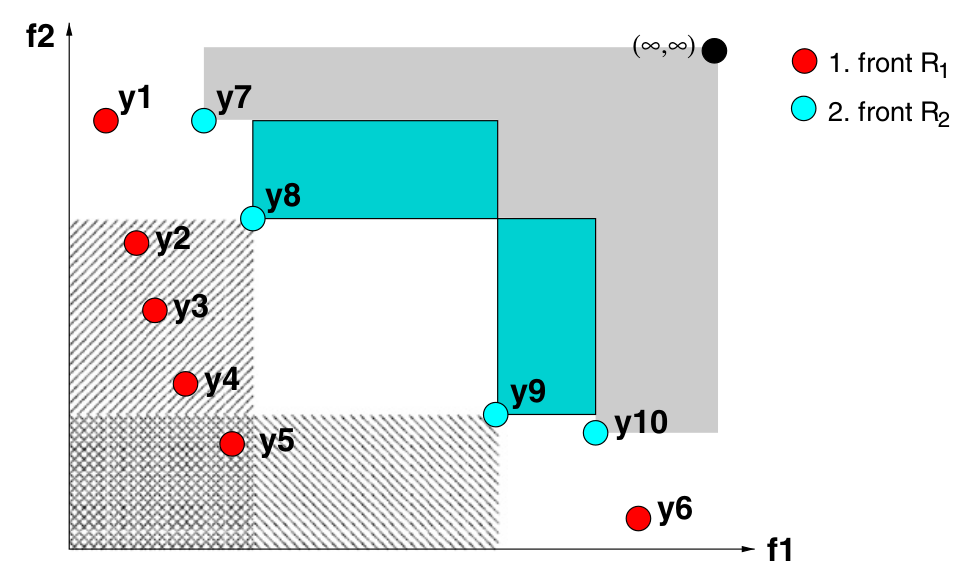
\includegraphics[scale=0.2]
{Figures_Chapter2/SMSEMOA_Fronts.png}
\decoRule
\caption{El hipervolumen dominado por el frente $\Re_2 = \{ y_7, . . ., y_{10} \}$ est\'a resaltado y sus contribuciones de $\Delta_{\mathscr{S}}(y_8,\Re_2)$ y  $\Delta_{\mathscr{S}}(y_9,\Re_2)$ se visualizan en los rect\'angulos con fondo verde. Las \'areas sombreadas corresponden a las regiones que contienen los puntos que dominan a $y_8$ y $y_9$ respectivamente.}
\label{fig:SMS-EMOA-HV}
\end{figure}


\begin{algorithm}[!t]
\caption{SMS-EMOA}
\label{alg:SMSEMOA}
\begin{scriptsize}
\begin{algorithmic}[1]
	\STATE $P_0 \leftarrow $ Inicializar la población de forma aleatoria en el espacio factible.
    \STATE $t \leftarrow 0$
    \WHILE{ Criterio de paro no cumplido}
    	\STATE $q_{t+1} \leftarrow $ Generar($P_t$) \Comment{Generar un individuo mediante un conjunto de operadores evolutivos.}
        \STATE $P_{t+1} \leftarrow $ Reducir($P_t \cup \{ q_{t+1} \} $) \Comment{Eliminar al individuo cuya aportación a la diversidad sea mínima.}
    	\STATE $t \leftarrow t+1$
    \ENDWHILE
\end{algorithmic}
\end{scriptsize}
\end{algorithm}

\subsection{Metaheurística de Muchos Objetivos Basada en el Indicador (R2 MOMBI-II)}


%
El MOMBI-II (\textit{Many Objective Metaheuristic Based on the R2 Indicator}) es un algoritmo basado en indicadores y utiliza el indicador $R2$ en el proceso de selección, este indicador es desarrollado como alternativa al hipervolumen, ya que en este último el costo computacional incrementa exponencialmente a razón del número de objetivos.
%
En este algoritmo se consideran dos aspectos clave: implementar una función de escalarización lograda en el transcurso de la ejecución y utilizar la información estadística sobre la proximidad entre la población y al frente óptimo de Pareto.
%
En la versión original del MOMBI se implementa la normalización de cada función objetivo utilizando la expresión:
\begin{equation*}
f^,_i(\vec{x}) = \frac{f_i(\vec{x}) - z_i^{min}}{ z_i^{max} - z_i^{min}}
\end{equation*}
donde $z^{\vec{min}}$ y $z^{\vec{max}}$ son los vectores ideal y nadir respectivamente de la población actual.
%
Sin embargo se ha observado principalmente los siguiente problemas:
\begin{itemize}
\item El vector ideal verdadero nunca es retenido, en consecuencia faltan las soluciones de los límites que corresponden al frente de Pareto.
\item Además en problemas multi-frontales, el vector nadir siempre es asignado a una solución atípica o aislada, causando una distribución pobre en las aproximaciones obtenidas.
\item En problemas de alta dimensionalidad en el espacio objetivo, puede presentarse la dificultad de que los vectores ideal y nadir estén muy cercanos por lo tanto existe una perdida de diversidad en el espacio objetivo. 
\end{itemize}
%
Para resolver las fallas previamente mencionadas en el MOMBI-II se toma en cuenta la información estadística de las generaciones previas, esto se logra monitoreando el desplazamiento del vector nadir, así una varianza elevada de este vector indica que las soluciones se encuentran alejadas del frente de Pareto, por otra parte una varianza pequeña indica que las soluciones están cercanas al frente de Pareto por lo que se deben realizar desplazamientos pequeños de este mismo vector.
%

Se implementa un procedimiento de clasificación descrito en el algoritmo \ref{alg:R2-Ranking-Algorithm}.
%
Así las soluciones que optimizan el conjunto de vectores de pesos son escogidos y son ubicados en la parte superior, de tal forma que obtienen el primer rango considerados como los mejores similar al procedimiento del Ordenación Eficiente de soluciones no dominadas del algoritmo NSGA-II.
%
En la notación se sugiere que cada individuo $p$ contiene el vector de funciones objetivo $p.\vec{f}$, la jerarquía de los individuos $p.rank$ y $p.\mu$, el valor de utilidad actual para el vector de pesos $\vec{w}$, la complejidad de este algoritmo es de $O(|W||P|(log |P| + m) )$.
%
La complejidad general en cada generación del procedimiento principal del MOMBI-II algoritmo \ref{alg:MOMBI-II}, es $O(|W||P|(log |P| + m) )$.
%
\begin{algorithm}[H]
\caption{Procedimiento principal del MOMBI-II}
\label{alg:MOMBI-II}
\begin{scriptsize}
\begin{algorithmic}[1]
	\STATE Inicializar población $P_i,i \leftarrow 1$
    \STATE Evaluar población $P_i$
    \STATE Calcular la norma $L_2$ de todos los objetivos para $P_i$
    \STATE Asignar $ \vec{z}^{min} \leftarrow \vec{z}^*$ y $\vec{z}^{max} \leftarrow \vec{z}^{nadir}$
    \WHILE{ Condición de paro no sea cumplida }
    	\STATE Realizar la selección de los padres
        \STATE Generar las soluciones hijo $P^,_i$ utilizan variación de operadores
        \STATE Evaluar a la población $P^,_i$
        \STATE Calcular la norma $L_2$ de los objetivos para $P^,_i$
        \STATE Normalizar las funciones objetivo para $P_i \cup P^,_i$
        \STATE Llamar al Algoritmo para calcular los rangos con $R2$ $(P_i \cup P^,_i, W)$
        \STATE Reducir la población $P_{i+1} \leftarrow \{P_i \cup P^,_i\}$
        \STATE Actualizar los puntos de referencia $(\vec{z}^{min}m \vec{z}^{max}, P_{i+1}, m)$
        \STATE $i \leftarrow i+1$
    \ENDWHILE
    \RETURN $P_i$
\end{algorithmic}
\end{scriptsize}
\end{algorithm}

%
\begin{algorithm}[H]
\caption{Algoritmo para calcular los rangos con $R2$}
\label{alg:R2-Ranking-Algorithm}
\begin{scriptsize}
\begin{algorithmic}[1]
	\STATE $p.rank \leftarrow p.\mu \Leftarrow \infty \forall p \in P $
    \FOR{Todo $\vec{w} \in W$}
    	\FOR{Todo $p \in P$}
        	\STATE $p.\mu \leftarrow u_{asf}(p.\vec{f}:\vec{0}, \vec{w})$
        \ENDFOR
        \STATE Ordenar $P$ por medio de los campos $\mu$ y $L_2$ en orden creciente 
    	\STATE $rank \leftarrow 1$
        \FOR{Todo $p \in P$}
        	\STATE $p.rank \leftarrow min\{ p.rank, rank \}$
			\STATE $rank \leftarrow rank+1$
		\ENDFOR
    \ENDFOR
\end{algorithmic}
\end{scriptsize}
\end{algorithm}

\subsection{Evolución Diferencial Generalizada (GDE3)}
El algoritmo de Evolución Diferencial Generalizado ( Generalized Differential Evolution - GDE3), es una extensión de Evolución Diferencial (DE) para optimización global con cualquier número de objetivos y restricciones.
%
La primera versión de GDE desarrollada para optimización multi-objetivo fue propuesto por medio de una regla de selección basada en DE (\cite{Joel:SelectionRuleLampinen}).
%
La idea básica en la regla de selección consiste en elegir arbitrariamente un vector para reemplazar a un vector antiguo  en la siguiente generación sólo si este domina débilmente al vector antiguo.
%
A pesar de que no se obtenían soluciones bien distribuidas en el frente de Pareto, la primera versión del GDE proporciona buenas soluciones, sin embargo esta vversión era muy sensible en la parametrización.
%
Posteriormente se realizó la modificación del GDE para realizar la regla de selección en base a la diversidad en el espacio objetivo en el caso especial de que el vector arbitrario y el vector antiguo fueran no dominados.
%
Sin embargo la segunda versión GDE2 era aún muy sensible al modificar los parámetros de control.
%
La tercera versión del GDE propuesta extiende el método \textit{DE/rand/1/bin} a problemas con $M$ objetivos y $K$ restricciones.
%
La selección en el GDE3 está basado en las siguientes reglas:
\begin{itemize}
\item En el caso de vectores no factibles, el vector arbitrario es seleccionado si domina débilmente al vector antiguo en el espacio restringido, de otra forma el vector antiguo es seleccionado.
\item En el caso de los vectores factibles y no factibles, el vector factible es seleccionado.
\item Si los dos vectores son factibles, entonces el vector arbitrario es seleccionado si domina débilmente al vector antiguo en el espacio objetivo. Si el vector antiguo domina al vector arbitrario, entonces el vector antiguo es seleccionado. Si los vectores no se dominan entre sí en el espacio objetivo, entonces los dos vectores son seleccionados para la siguiente generación.
\end{itemize}
Después de cada generación puede haberse incrementado el tamaño de la población solo si el vector arbitrario y el antiguo son factibles, y además no se dominan mutuamente, si este es el caso entonces la población es reducida al tamaño original con un enfoque similar a la selección utilizada en el NSGA-II.


\begin{algorithm}[H]
\caption{Evolución Diferencia Generalizada GDE3}
\scriptsize
\label{alg:GDE3}
\begin{scriptsize}
\begin{algorithmic}[1]
	\WHILE{Criterio de parada no sea cumplido}
	\STATE $k=1$
	\FOR{ $i \in N$}
    	\STATE Mutar y recombinar:
    	   %\begin{ALC@g}
    	      \STATE Seleccionar aleatoriamente $r_1, r_2, r_3 \in \{ 1,2, ..., N \} \neq i$
    	      \STATE Seleccionar aleatoriamente $j_{rand} \in \{1, 2, ..., D \}$
    	      \FOR{$j \in D$}
    	 	       \IF{$rand_j[0,1) < CR \lor j == j_{rand}$} 
    		      		\STATE $u_{j,i, G}=x_{j,r_3, G} + F \cdot (x_{j, r_1, G} - x_{j, r_2, G})$
    	   	  	 	\ELSE
    	      			\STATE   $u_{j,i, G}= x_{j,i,G}$
    	   		   \ENDIF
    	      %		\STATE $  u_{j,i, G} = \begin{cases} x_{j,r_3, G} + F \cdot (x_{j, r_1, G} - x_{j, r_2, G}) & si \quad rand_j[0,1) < CR \lor j == j_rand \\ x_{j,i,G} de \quad otra \quad forma   \end{cases}$
    	      \ENDFOR
    	      \IF{$\vec{u}_{i,G} \preceq_c \vec{x}_{i,G}$}   
    	         \STATE $\vec{x}_{i, G+1 } =\vec{u}_{i,G}$ 
    	      \ELSE 
    	          \STATE $\vec{x}_{i, G+1 }= \vec{x}_{i,G}$
    	      \ENDIF
%			   \STATE Seleccionar $ \vec{x}_{i, G+1 } =  \begin{cases} \vec{u}_{i,G} & si \quad \vec{u}_{i,G} \preceq_c \vec{x}_{i,G}  \\ \vec{x}_{i,G} & de \quad otra \quad forma \end{cases}$    	 
			   \IF{ $\{\forall z : g_z (\vec{u}_i,G) \leq 0 \} \land \{ \vec{x}_{i, G+1} == \vec{x}_{i,G} \} \land \{ \vec{x}_{i,G} \nprec  \vec{u}_{i,G} \}$}
			   \STATE $\vec{x}_{N+k, G+1} = \vec{u}_{i,G}$   
				\STATE $k=k+1$
			   \ENDIF
    	   %\end{ALC@g}
	\ENDFOR
	\STATE $P$ = Ordenación Eficiente basado en No dominados($\vec{x}_{ 1:N+k,G+1}$)
	\STATE Eliminar los $k$ peores individuos de $P$ basado en el criterio del peor rango y de amontonamiento, similar al NSGA-II
    \ENDWHILE
\end{algorithmic}
\end{scriptsize}
\end{algorithm}

%----------------------------------
\section{Problemas de Prueba}
Como parte de la validación experimental de este trabajo y con el objetivo de tener un amplio panorama de las propiedades que poseen los algoritmos propuestos, se describen algunos de los problemas de prueba más populares en el ámbito multi-objetivo.
%
Se hace énfasis que en este trabajo no se consideran restricciones, por lo que los problemas de prueba escogidos son libres de restricciones, además están conformados por dominios  continuos.
%
Uno de los primeros problemas de prueba propuestos en multi-objetivo son los mencionados ZDT (\cite{Joel:ZDT}), los cuales están basados en tres funcionales para controlar la forma y posición del frente de Pareto óptimo.
%
Sin embargo este conjunto de problemas únicamente son diseñados para dos objetivos y no implementan características deceptivas en dominios continuos.
%

Posteriormente se propusieron los problemas DTLZ (\cite{Joel:DTLZ_2}), los cuales son escalables en el espacio objetivo y ofrecen problemas de prueba especiales para algoritmos diseñados en optimización de muchos objetivos.
%
Sin embargo existen ciertas limitaciones: no se presentan problemas deceptivos, tampoco se proporcionan problemas no separables y el número de parámetros son fijos en relación al número de objetivos.
%

En ese orden, un generador o toolkit de problemas multi-objetivo fue propuesto por \cite{Joel:WFG}, conocido como \textit{The Walking Fish Group} (WFG) siendo nueve problemas de ejemplo, entre los cuales varios son similares a los DTLZ,  y otros son considerados como problemas de mayor complejidad que los ZDT y DTLZ. 
%
La escalabilidad tanto en el espacio de las variables como en el espacio objetivo, hace viable implementar estas funciones de ejemplo como problemas de prueba. 

%
Más recientemente, en el Congreso de Cómputo Evolutivo del 2009 (CEC09) se propusieron los problemas UF, entre los cuales existen problemas con restricciones y sin restricciones, principalmente los problemas sin restricciones están descritos únicamente de dos y tres objetivos, sin embargo representan un reto en base a su dificultad, por lo que en la actualidad aún son utilizados como parte de la validación de distintos trabajos en el ámbito multi-objetivo.

\subsection{ZDT}
Los problemas conocidos como ZDT fueron propuestos por sus autores~\cite{Joel:ZDT}, surgen con el propósito de comparar distintos aspectos de los MOEAs.
%
Las funciones propuestas incluyen convexidad, no convexidad, frentes de Pareto discretos, multi-modalidad, deceptividad (en codificación binaria) y espacios de búsqueda sesgados.
%
Estos problemas están estructurados únicamente para dos objetivos, y cada función de prueba consiste de tres funciones $f_1$, $g$ y $h$.
%
Donde $f_1$ es una función utilizada en la primer variable de decisión, $g$ es implementada para las siguientes $n-1$ variables, y los parámetros de $h$ son los valores que corresponden a las funciones $f_1$ y $g$.
%
Las funciones de prueba difieren en estas tres funciones como en el número de variables $n$, y en los valores que las variables pueden tomar.
%
Desde que la función de prueba ZDT5 está representada codificación binaria es ignorada.
%
La descripción detallada de cada uno de los problemas se enlista a continuación y la definición de los mismos se ubica en la tabla \ref{tab:ZDT}.

\subsubsection*{Función de prueba ZDT1}
Esta función de prueba tiene un frente óptimo de Pareto convexo.
%\begin{equation}
%\begin{split}
%f_1(x_1) &= x_1 \\
%g(x_2, ..., x_n) &= 1+9  \sum_{i=2}^n x_i / (n-1) \\
%h(f_1, g) &= 1 - \sqrt{f_1/g}
%\end{split}
%\end{equation}
El número de variables normalmente usado es $n=30$, y $x_i \in [0,1]$. El frente de Pareto óptimo es formado con $g(x)=1$.

\subsubsection*{Función de prueba ZDT2}
Esta función de prueba tiene un frente de Pareto optimo no convexo.
%\begin{equation}
%\begin{split}
%f_1(x_1) &= x_1 \\
%g(x_2, ..., x_n) &= 1+9  \sum_{i=2}^n x_i / (n-1) \\
%h(f_1, g) &= 1 - (f_1/g)^2
%\end{split}
%\end{equation}
El número de variables normalmente usado es $n=30$, y $x_i \in [0,1]$. El frente de Pareto óptimo es formado con $g(x)=1$.

\subsubsection*{Función de prueba ZDT3}
Esta función de prueba el frente de Pareto óptimo consiste de varias partes convexas y no continuas.
%\begin{equation}
%\begin{split}
%f_1(x_1) &= x_1 \\
%g(x_2, ..., x_n) &= 1+9  \sum_{i=2}^n x_i / (n-1) \\
%h(f_1, g) &= 1 - \sqrt{f_1/g} - (f_1 / g) sin( 10 \pi f_1)
%\end{split}
%\end{equation}
El número de variables es normalemente usado es $n=30$, y $x_i \in [0,1]$. El frente de Pareto óptimo es formado con $g(x)=1$.
%
La función senoidal en la función $h$ causan una discontinuidad en el frente de Pareto óptimo.
%
Sin embargo no existe una discontinuidad en el espacio de las variables.

\subsubsection*{Función de prueba ZDT4}
Esta función de prueba contiene $21^9$ frentes de Pareto óptimos locales y, prueba la capacidad de tratar problemas con multi-modalidad.
%\begin{equation}
%\begin{split}
%f_1(x_1) &= x_1 \\
%g(x_2, ..., x_n) &= 1 + 10(n-1) + \sum_{i=2}^n (x_i^2 - 10 cos( 4 \pi x_i)) \\
%h(f_1, g) &= 1 - \sqrt{f_1/g}
%\end{split}
%\end{equation}
El número de variables normalmente usado es $n=10$, y $x_1 \in [0,1]$, y $x_2, ..., x_n \in [-5, 5]$. El frente de Pareto óptimo global es formado con $g(x)=1$.
%
El mejor frente óptimo de Pareto local se forma con $f(x)=1.25$

\subsubsection*{Función de prueba ZDT6}
Esta función de prueba incluye dos dificultades causadas por la no uniformidad del espacio de búsqueda. Primeramente, las soluciones óptimas de Pareto est\'an distribuidas de forma no uniforme, provocando una mayor densidad para valores donde $f_1$ es cercano a uno; segundo: la densidad de las soluciones es menor cerca del frente de Pareto óptimo y mayor alejadas del frente.
%\begin{equation}
%\begin{split}
%f_1(x_1) &= 1 - exp(-4 x_1) sin^6 (6 \pi x_1) \\
%g(x_2, ..., x_n) &= 1 + 9 \sum_{i=2}^n (x_i / (n-1))^{0.25} \\
%h(f_1, g) &= 1 - (f_1/g)^2
%\end{split}
%\end{equation}
El número de variables normalmente usadi es $n=10$, y $x_i \in [0,1]$. El frente de Pareto óptimo es formado con $g(x)=1$.
%
La forma del frente de Pareto óptimo es no convexo.


% Please add the following required packages to your document preamble:
% \usepackage{graphicx}
\begin{table}[H]
\centering
\caption{Problemas ZDT}
\label{tab:ZDT}
\resizebox{\textwidth}{!}{%
\begin{tabular}{|c|l|c|}
\hline
Nombre & \multicolumn{1}{c|}{Problema} & Dominio de los parámetros \\ \hline
ZDT1 & $ \begin{array}{lll} f_1(x_1) &= x_1 \\g(x_2, ..., x_n) &= 1+9,\sum_{i=2}^n x_i / (n-1) \\h(f_1, g) &= 1 - \sqrt{f_1/g} \end{array}$ & $[0,1]$ \\ \hline
ZDT2 & Igual que ZDT1, a excepción de $h = 1-(f_1 / g)^2$ & $[0,1]$ \\ \hline
ZDT3 & Igual que ZDT1, a excepción de $h(f_1, g) = 1 - \sqrt{f_1/g} - (f_1 / g) sin( 10 \pi f_1)$ & $[0,1]$ \\ \hline
ZDT4 & Igual que ZDT1, a excepción de $h(f_1, g) = 1 - \sqrt{f_1/g}$ & $ \begin{array}{lll}  x_1 \in [0,1] \\ x_2, ..., x_n \in [-5, 5] \end{array}$ \\ \hline
ZDT6 & $ \begin{array}{lll} f_1(x_1) &= 1 - exp(-4 x_1) sin^6 (6 \pi x_1) \\g(x_2, ..., x_n) &= 1 + 9 \sum_{i=2}^n (x_i / (n-1))^{0.25} \\h(f_1, g) &= 1 - (f_1/g)^2 \end{array}$ & $[0,1]$ \\ \hline
\end{tabular}%
}
\end{table}

\subsection{DTLZ}
El conjunto de problemas propuesto por \cite{Joel:DTLZ_1, Joel:DTLZ_2}, está conformado por nueve instancias, diseñados para probar distintas propiedades de los MOEAs.
%
A diferencia de los problemas ZDT, estos problemas son escalables, además de que ofrecen nuevas características, como es  el caso de los problemas de prueba degenerados DTLZ5 y DTLZ6.
%
La descripción detallada de cada uno de los problemas se enlista a continuación, la definición de los mismos se ubica en la tabla \ref{tab:DTLZ} y el gráfico que corresponde al óptimo de Pareto en tres objetivos en la figura \ref{fig:DTLZ}.

\subsubsection*{Función de prueba DTLZ1}
Esta función de prueba es separable y es multi-modal.
%\begin{equation}
%\scriptsize
%\begin{split}
%& Minimizar \quad f_1(\mathbf{x}) = \frac{1}{2} x_1 x_2 . . . x_{M-1} (1+g(\mathbf{x}_M)),\\
%& Minimizar \quad f_2(\mathbf{x}) = \frac{1}{2} x_1 x_2 . . . (1 - x_{M-1}) (1+g(\mathbf{x}_M)),\\
%&..\\
%& Minimizar \quad f_{M-1}(\mathbf{x}) = \frac{1}{2} x_1 (1-x_2)(1+g(\mathbf{x}_M)),\\
%& Minimizar \quad f_{M}(\mathbf{x}) = \frac{1}{2} (1-x_1)(1+g(\mathbf{x}_M)),\\
%& sujeto\quad a \quad 0 \leq x_i \leq 1, \quad for \quad i=1,2,...,n
%\end{split}
%\end{equation}
%
%El funcional $g(\mathbf{x_M})$ requiere $|\mathbf{x}_M| = k$ variables, y deben evaluarse con $g \geq 0$.
%%
%Se sugiere:
%\begin{equation*}
%g(\mathbf{x}_M) = 100 \left[ |\mathbf{x}_M| + \sum_{x_i \in \mathbf{x}_M} (x_i = 0.5)^2 - cos(20 \pi (x_i - 0.5 )) \right ]
%\end{equation*}
El frente de Pareto óptimo requiere que $\mathbf{x}_M = 0$ el cual corresponde en el espacio objetivo a un hiperplano lineal $\sum_{m=1}^M f_m - 0.5$.
%
Se sugiere un valor de $k=5$ y el número de variables es denotado por $n=M+k-1$.
%
La dificultad de este problema es la convergencia al hiperplano ya que el espacio de búsqueda contiene ($11^k - 1$) frentes óptimos de Pareto locales.
%
Se puede reestructurar un problema más complicado implementando funciones $g$ multi-modales, reemplazando $x_i$ por un mapeo no lineal $x_i= N_i(y_i)$ y tratando $y_i$ como una variable. 

\subsubsection*{Función de prueba DTLZ2}
%\begin{equation}
%\scriptsize
%\begin{split}
%& Minimizar \quad f_1(\mathbf{x}) = (1+g(\mathbf{x}_M)) cos(x_1 \pi /2) cos(x_2 \pi /2) . . . cos(x_{M-2} \pi /2) cos(x_{M-1} \pi /2) ,\\
%& Minimizar \quad f_2(\mathbf{x}) = (1+g(\mathbf{x}_M)) cos(x_1 \pi /2) cos(x_2 \pi /2) . . . cos(x_{M-2} \pi /2) sin(x_{M-1} \pi /2) ,\\
%& Minimizar \quad f_3(\mathbf{x}) = (1+g(\mathbf{x}_M)) cos(x_1 \pi /2) cos(x_2 \pi /2) . . . sin(x_{M-2} \pi /2) ,\\
%&....\\
%& Minimizar \quad f_{M-1}(\mathbf{x}) = (1+g(\mathbf{x}_M)) cos(x_1 \pi /2) sin(x_2 \pi /2),\\
%& Minimizar \quad f_{M}(\mathbf{x}) = (1+g(\mathbf{x}_M))sin(x_1 \pi /2)\\
%& sujeto\quad a \quad 0 \leq x_i \leq 1, \quad for \quad i=1,2,...,n\\
%\end{split}
%\end{equation}
%donde 
%\begin{equation*}
%\begin{split}
%g(\mathbf{x}_M) = \sum_{x_i \in \mathbf{x}_M} (x_i - 0.5)^2
%\end{split}
%\end{equation*}
Las soluciones óptimas de Paretocorresponden a $x^*_M = 0.5$, se recomienda que $k=|\mathbf{x}_M| = 10$, y el número total de variables de $n=M+k-1$.
%
El frente de Pareto es no convexo, en el caso de tres objetivos las soluciones óptimas corresponden al primer cuadrante de una esfera unitaria. 
%
En el caso generalizado las soluciones óptimas están descritas por $\sum_{m=1}^M f_m^2 = 1$, que es representado por una hiperesfera unitaria ubicada en el origen.
%

\subsubsection*{Función de prueba DTLZ3}

%\begin{equation}
%\scriptsize
%\begin{split}
%& Minimizar \quad f_1(\mathbf{x}) = (1+g(\mathbf{x}_M)) cos(x_1 \pi /2) cos(x_2 \pi /2) . . . cos(x_{M-2} \pi /2) cos(x_{M-1} \pi /2) ,\\
%& Minimizar \quad f_2(\mathbf{x}) = (1+g(\mathbf{x}_M)) cos(x_1 \pi /2) cos(x_2 \pi /2) . . . cos(x_{M-2} \pi /2) sin(x_{M-1} \pi /2) ,\\
%& Minimizar \quad f_3(\mathbf{x}) = (1+g(\mathbf{x}_M)) cos(x_1 \pi /2) cos(x_2 \pi /2) . . . sin(x_{M-2} \pi /2) ,\\
%&....\\
%& Minimizar \quad f_{M-1}(\mathbf{x}) = (1+g(\mathbf{x}_M)) cos(x_1 \pi /2) sin(x_2 \pi /2),\\
%& Minimizar \quad f_{M}(\mathbf{x}) = (1+g(\mathbf{x}_M))sin(x_1 \pi /2)\\
%& sujeto\quad a \quad 0 \leq x_i \leq 1, \quad for \quad i=1,2,...,n\\
%\end{split}
%\end{equation}
%donde 
%\begin{equation*}
%g(\mathbf{x}_M) = 100 \left[ |\mathbf{x}_M| + \sum_{x_i \in \mathbf{x}_M} (x_i = 0.5)^2 - cos(20 \pi (x_i - 0.5 )) \right ]
%\end{equation*}

En este problema se sugiere $k= | \mathbf{x}_M| =  10$, con un número de variables de $n = M + k -1$.
%
La función $\mathbf{g}$ introduce $( 3^k - 1)$ óptimos locales del frente de Pareto y óptimos globales del frente de Pareto.
%
Los óptimos locales del frente de Pareto son paralelos a los óptimos globales del frente de Pareto, por lo tanto el MOEA puede generar soluciones y estancarse en los óptimos locales del frente de Pareto.
%
El frente de Pareto óptimo global corresponde a $\mathbf{x}_M = (0.5, ..., 0.5)^T$ (en $g^* = 0$)
%
En este problema prueba la capacidad de un MOEA para obtener soluciones bien distribuídas y se basa en el problema DTLZ2, con una asignaci\'on o mapeo de las metavariables.
%\begin{equation}
%\scriptsize
%\begin{split}
%& Minimizar \quad f_1(\mathbf{x}) = (1+g(\mathbf{x}_M)) cos(x_1^{\alpha} \pi /2) cos(x_2^{\alpha} \pi /2) . . . cos(x_{M-2}^{\alpha} \pi /2) cos(x_{M-1}^{\alpha} \pi /2) ,\\
%& Minimizar \quad f_2(\mathbf{x}) = (1+g(\mathbf{x}_M) cos(x_1^{\alpha} \pi /2) cos(x_2^{\alpha} \pi /2) . . . cos(x_{M-2}^{\alpha} \pi /2) sin(x_{M-1}^{\alpha} \pi /2) ,\\
%& Minimizar \quad f_3(\mathbf{x}) = (1+g(\mathbf{x}_M)) cos(x_1^{\alpha} \pi /2) cos(x_2^{\alpha} \pi /2) . . . sin(x_{M-2}^{\alpha} \pi /2) ,\\
%&....\\
%& Minimizar \quad f_{M-1}(\mathbf{x}) = (1+g(\mathbf{x}_M)) cos(x_1^{\alpha} \pi /2) sin(x_2^{\alpha} \pi /2),\\
%& Minimizar \quad f_{M}(\mathbf{x}) = (1+g(\mathbf{x}_M))sin(x_1^{\alpha} \pi /2)\\
%& sujeto\quad a \quad 0 \leq x_i \leq 1, \quad for \quad i=1,2,...,n\\
%\end{split}
%\end{equation}
%donde 
%\begin{equation*}
%\begin{split}
%g(\mathbf{x}_M) = \sum_{x_i \in \mathbf{x}_M} (x_i - 0.5)^2
%\end{split}
%\end{equation*}
Se sugiere utilizar un valor de $\alpha = 100$ y $k=10$.
%
El n\'umero de variables es de $n=M+k-1$.
%
Esta modificación presenta una densidad del conjunto de soluciones cercano del plano $f_M - f_1$, sin embargo esta dificultad puede no presentarse en métodos lo cuales implementan enfoques como agregación de pesos y otros métodos direccionales.


\subsubsection*{Función de prueba DTLZ5}
%En este problema se implementa un cambio
%\begin{equation}
%\scriptsize
%\begin{split}
%& Minimizar \quad f_1(\mathbf{x}) = (1+g(\mathbf{x}_M)) cos(\theta_1 \pi /2) cos(\theta_2 \pi /2) . . . cos(\theta_{M-2} \pi /2) cos(\theta_{M-1} \pi /2) ,\\
%& Minimizar \quad f_2(\mathbf{x}) = (1+g(\mathbf{x}_M)) cos(\theta_1 \pi /2) cos(\theta_2 \pi /2) . . . cos(\theta_{M-2} \pi /2) sin(\theta_{M-1} \pi /2) ,\\
%& Minimizar \quad f_3(\mathbf{x}) = (1+g(\mathbf{x}_M)) cos(\theta_1 \pi /2) cos(\theta_2 \pi /2) . . . sin(\theta_{M-2} \pi /2) ,\\
%&....\\
%& Minimizar \quad f_{M-1}(\mathbf{x}) = (1+g(\mathbf{x}_M)) cos(\theta_1 \pi /2) sin(\theta_2 \pi /2),\\
%& Minimizar \quad f_{M}(\mathbf{x}) = (1+g(\mathbf{x}_M))sin(\theta_1 \pi /2)\\
%& sujeto\quad a \quad 0 \leq x_i \leq 1, \quad for \quad i=1,2,...,n\\
%\end{split}
%\end{equation}
%donde 
%\begin{equation*}
%\begin{split}
%\theta_i = \frac{\pi}{4(1+g(r))}(1+2g(r)x_i), \quad for \quad i=2,3,...,(M-1),\\
%g(\mathbf{x}_M) = \sum_{x_i \in \mathbf{x}_M} (x_i - 0.5)^2
%\end{split}
%\end{equation*}

En este problema se sugiere implementar la función $g$ con un número de variables $k = |\mathbf{x}_M| = 10$.
%
Este problema prueba la habilidad del MOEA para converger a una curva, y también permite una forma fácil de visualizar el frente óptimo en con cualquier número de objetivos asignados (sólo graficando $f_M$ con cualquier función objetivo).
%
Aunque es un problema sencillo, se sugiere implementarse con un numero de objetivos elevado ($M \in [5, 10]$) para estudiar la complejidad computacional de un MOEA.

\subsubsection*{Función de prueba DTLZ6}
Este problema consiste en modificar la función de prueba DTLZ5 asignando la función $g$ como:
\begin{equation*}
 g( \mathbf{x_M}) = \sum_{x_i \in \mathbf{x}_M} x_i^{0.1}
\end{equation*}
%
El cambio de la función $g$ dificulta que la soluciones tengan una convergencia en el frente de Pareto óptimo, el cual es una curva.

\subsubsection*{Función de prueba DTLZ7}
Esta función de prueba conforma regiones desconectadas en el frente de Pareto óptimo.
%\begin{equation*}
%\scriptsize
%\begin{split}
%&Minimizar \quad f_1(\mathbf{x_1}) = x_1,\\
%&Minimizar \quad f_2(\mathbf{x_2}) = x_2,\\
%&...\\
%&Minimizar \quad f_{M-1}( \mathbf{x}_M{M-1} ) = x_{M-1},\\
%&Minimizar \quad f_M(\mathbf{x}) = (1+ g(\mathbf{x}_M)) h(f_1, f_2, ..., f_{M-1}, g)\\
%&sujeto \quad a \quad 0 \leq x_i \leq 1 \quad for \quad i=1,2,...,n
%\end{split}
%\end{equation*}
%donde
%\begin{equation*}
%\begin{split}
%g(\mathbf{x}_M) = 1 + \frac{9}{| \mathbf{x}_M |} \sum_{x_i \in \mathbf{x}_M } x_i ,\\
%h(f_1, f_2,..., f_{M-1}, g) = M - \sum_{i=1}^{M-1} \left [ \frac{f_i}{1+g} (1 + sin( 3 \pi f_i )),  \right ]
%\end{split}
%\end{equation*}
%
Este problema de prueba tiene $2^{M-1}$ regiones de Pareto óptimos desconectadas en el espacio de búsqueda.
%
Las soluciones del frente de Pareto óptimo corresponden a $\mathbf{x}_M = 0$.
%
Este problema de prueba está diseñado para verificar la capacidad del MOEA de mantener subpoblaciones en distintas regiones que corresponden a óptimos de Pareto. 
\\ \\
Es importante hacer mención que en las instancias DTLZ6 y DTLZ7 el punto óptimo se encuentra en los límites del espacio de las variables, y como se indica por \citeauthor{Joel:ComparativoDEMO_FalloDTLZ6}, los algoritmos que generan soluciones fuera de los límites y cuyo método de reparación consiste en ubicar esta soluciones en los límites, resuelven este tipo de instancias de forma sencilla, esto es más evidente en algoritmos que implementan evolución diferencial como es el caso del GDE3 y del DEMO (\cite{Joel:ComparativoDEMO_FalloDTLZ6}), entre otros.
%
Específicamente se han observado los principales inconvenientes en las instancias ZDT y DTLZ \citep{Joel:CEC2009}:
\begin{itemize}
\item Para todos los problemas, el óptimo global tiene los mismos valores de parámetros para distintas variables/dimensiones.
\item El óptimo global está ubicado en el centro del espacio de búsqueda.
\item El óptimo global está ubicado en los límites.
\item Todos estos problemas son separables.
\end{itemize}
Se han propuesto correcciones a los problemas implementado rotaciones, desplazando puntos óptimos y expandiendo el espacio de búsqueda, sin embargo para implementar estos cambios se necesita información extra la cual es proporcionada mediante ficheros, entre estos son: vectores de desplazamiento en el espacio de los parámetros, un vector usado para expandir el límite inferior, un vector que corresponde al factor de escala, valores de penalización y una matriz de rotación.
%
Esta información sólo se ha proporcionado para los problemas S\_DTLZ2 y R\_DTLZ2 como modificaciones del DTLZ2, S\_DTLZ3 y R\_DTLZ3 del DTLZ3 en el Congreso de Cómputo Evolutivo 2007. Recientemente en R2\_DTLZ2\_M5 como modificación del DTLZ2 con 5 objetivos y R2\_DTLZ3\_M5 del DTLZ3 con 5 objetivos propuestos en el Congreso de Cómputo Evolutivo 2009. 

\begin{figure}[H]
\centering
\scriptsize
\caption{Frente de Pareto en tres objetivos de los problemas DTLZ}
\label{fig:DTLZ}
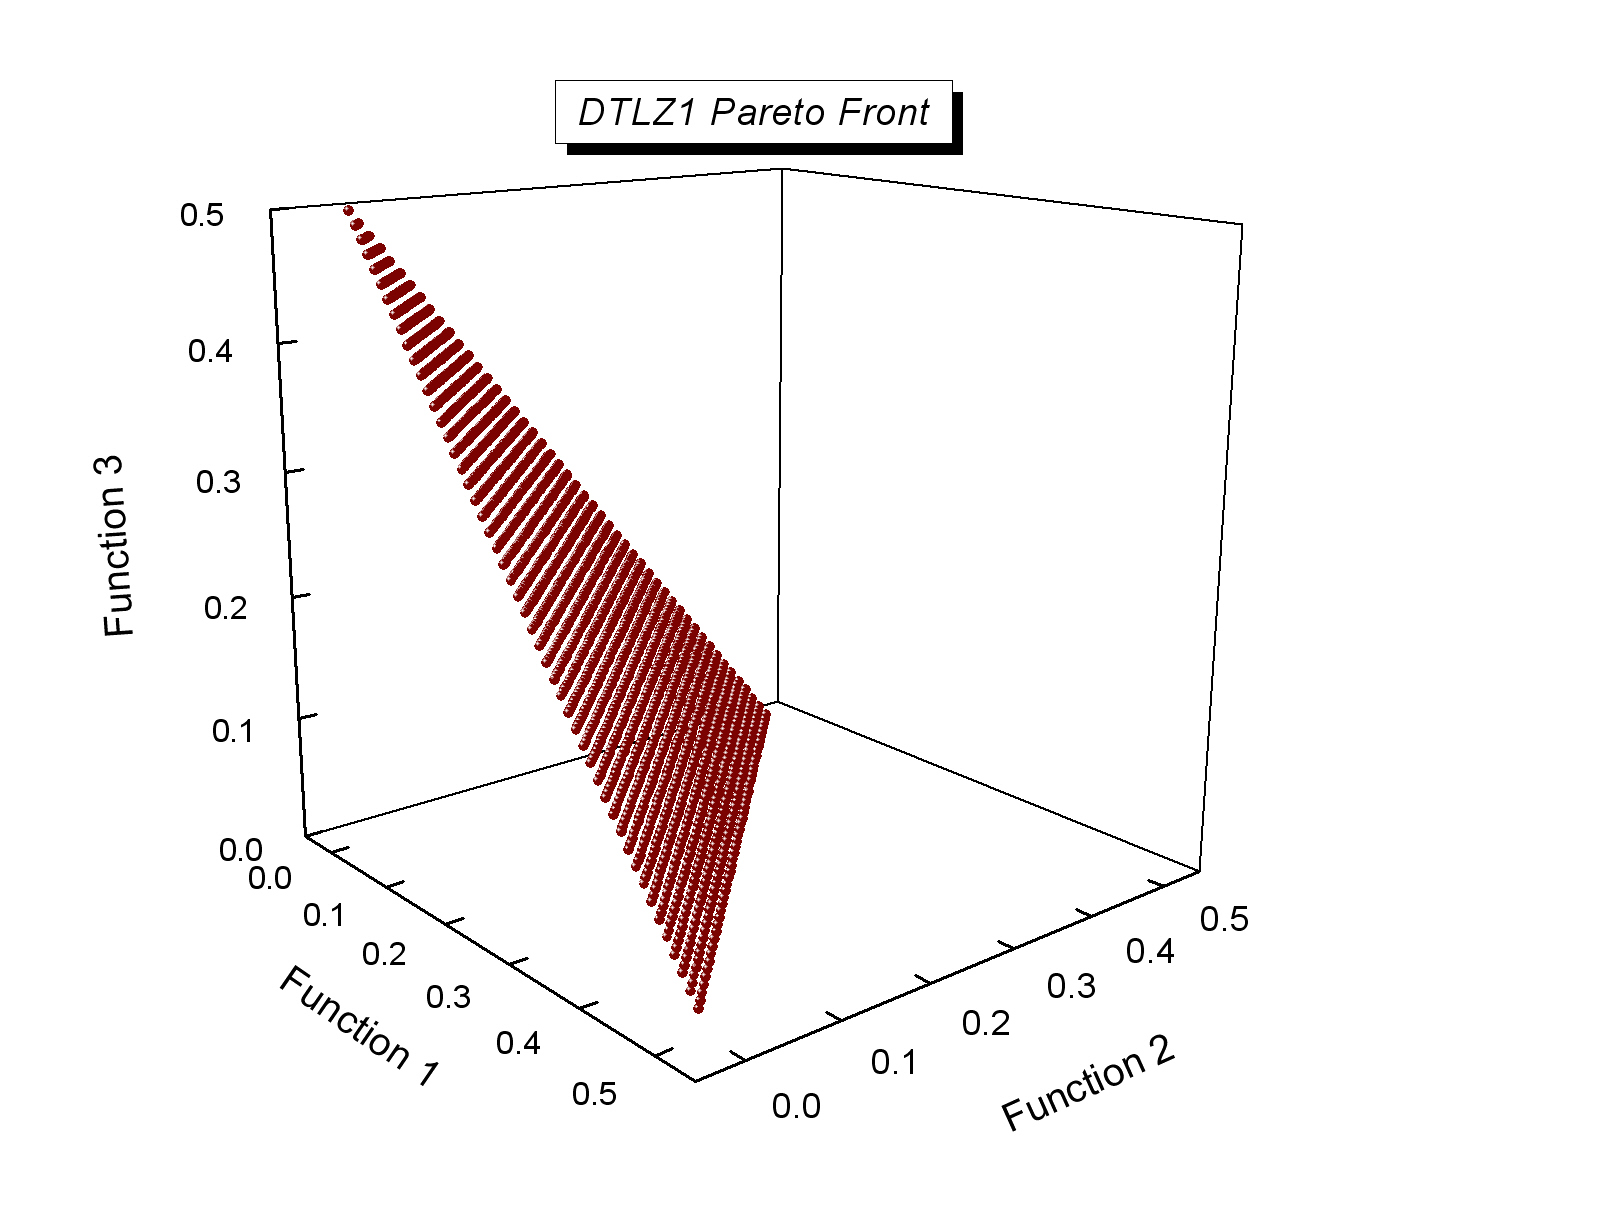
\includegraphics[scale=0.2]
{Figures_Chapter2/DTLZ1.jpg}
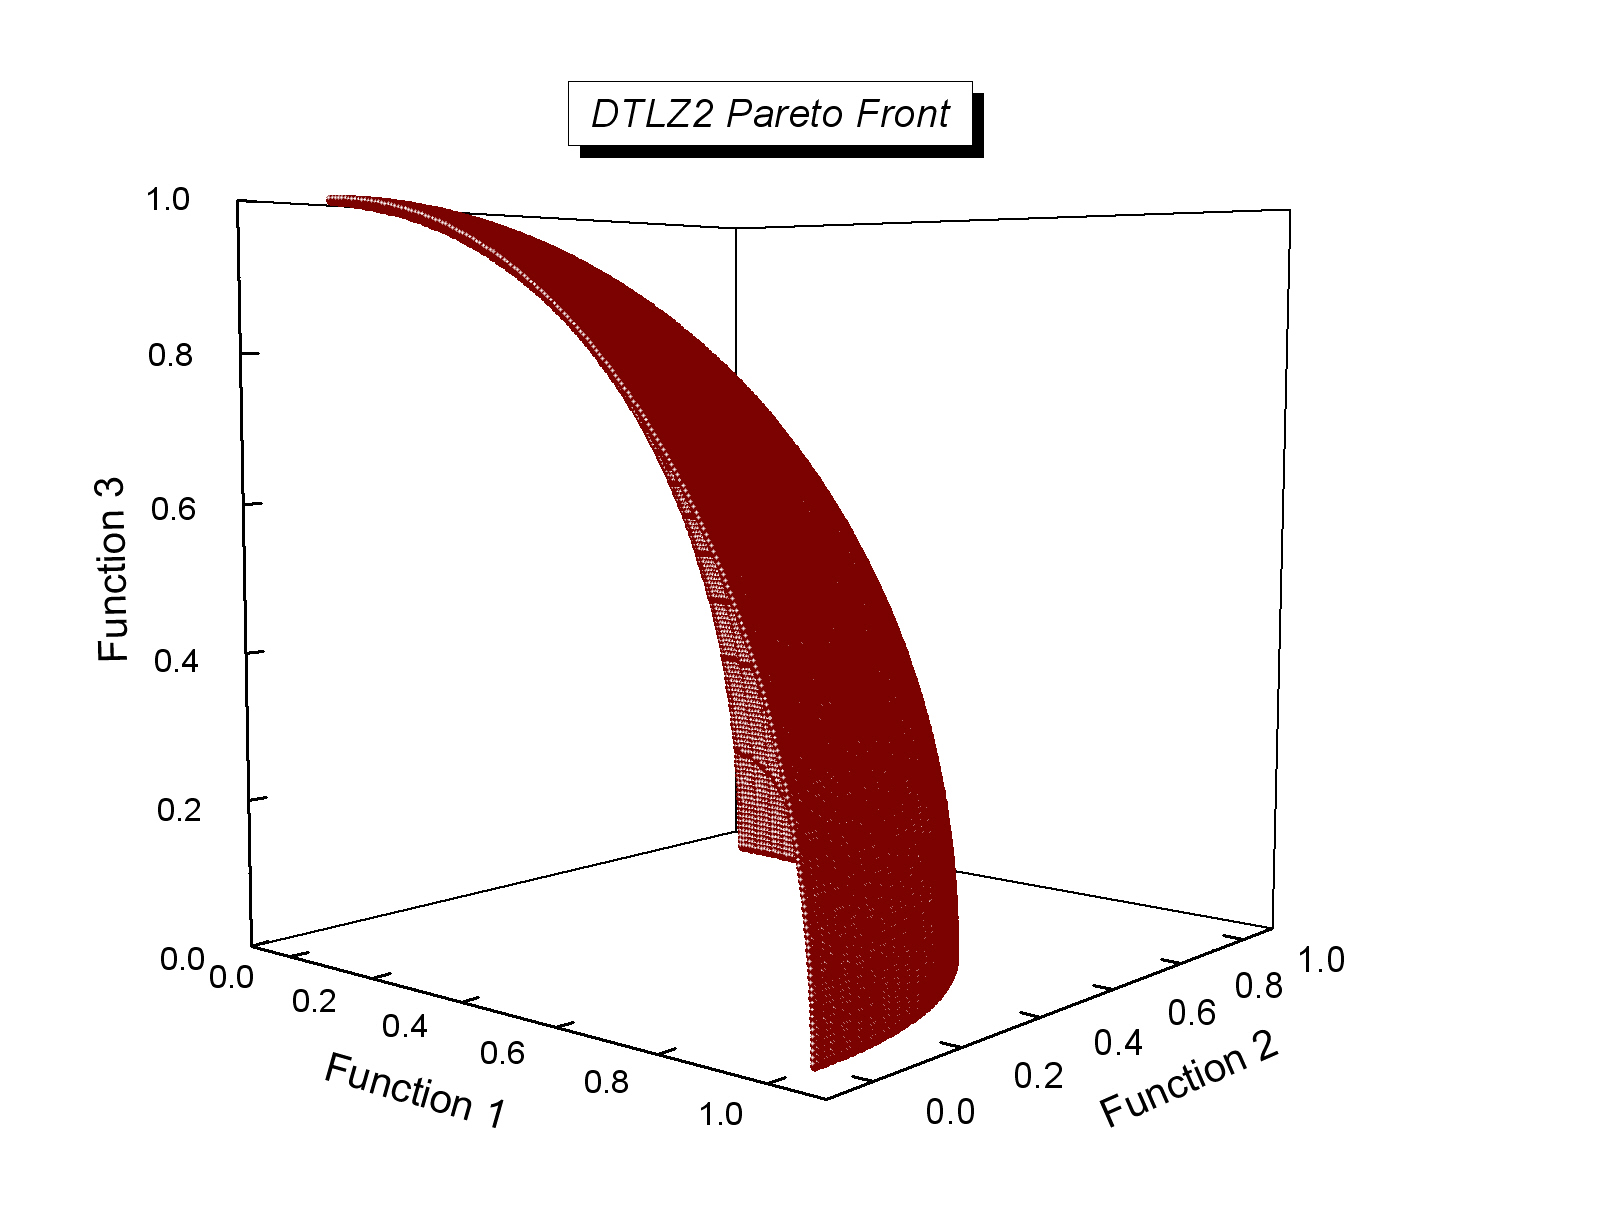
\includegraphics[scale=0.2]
{Figures_Chapter2/DTLZ2.jpg} \\
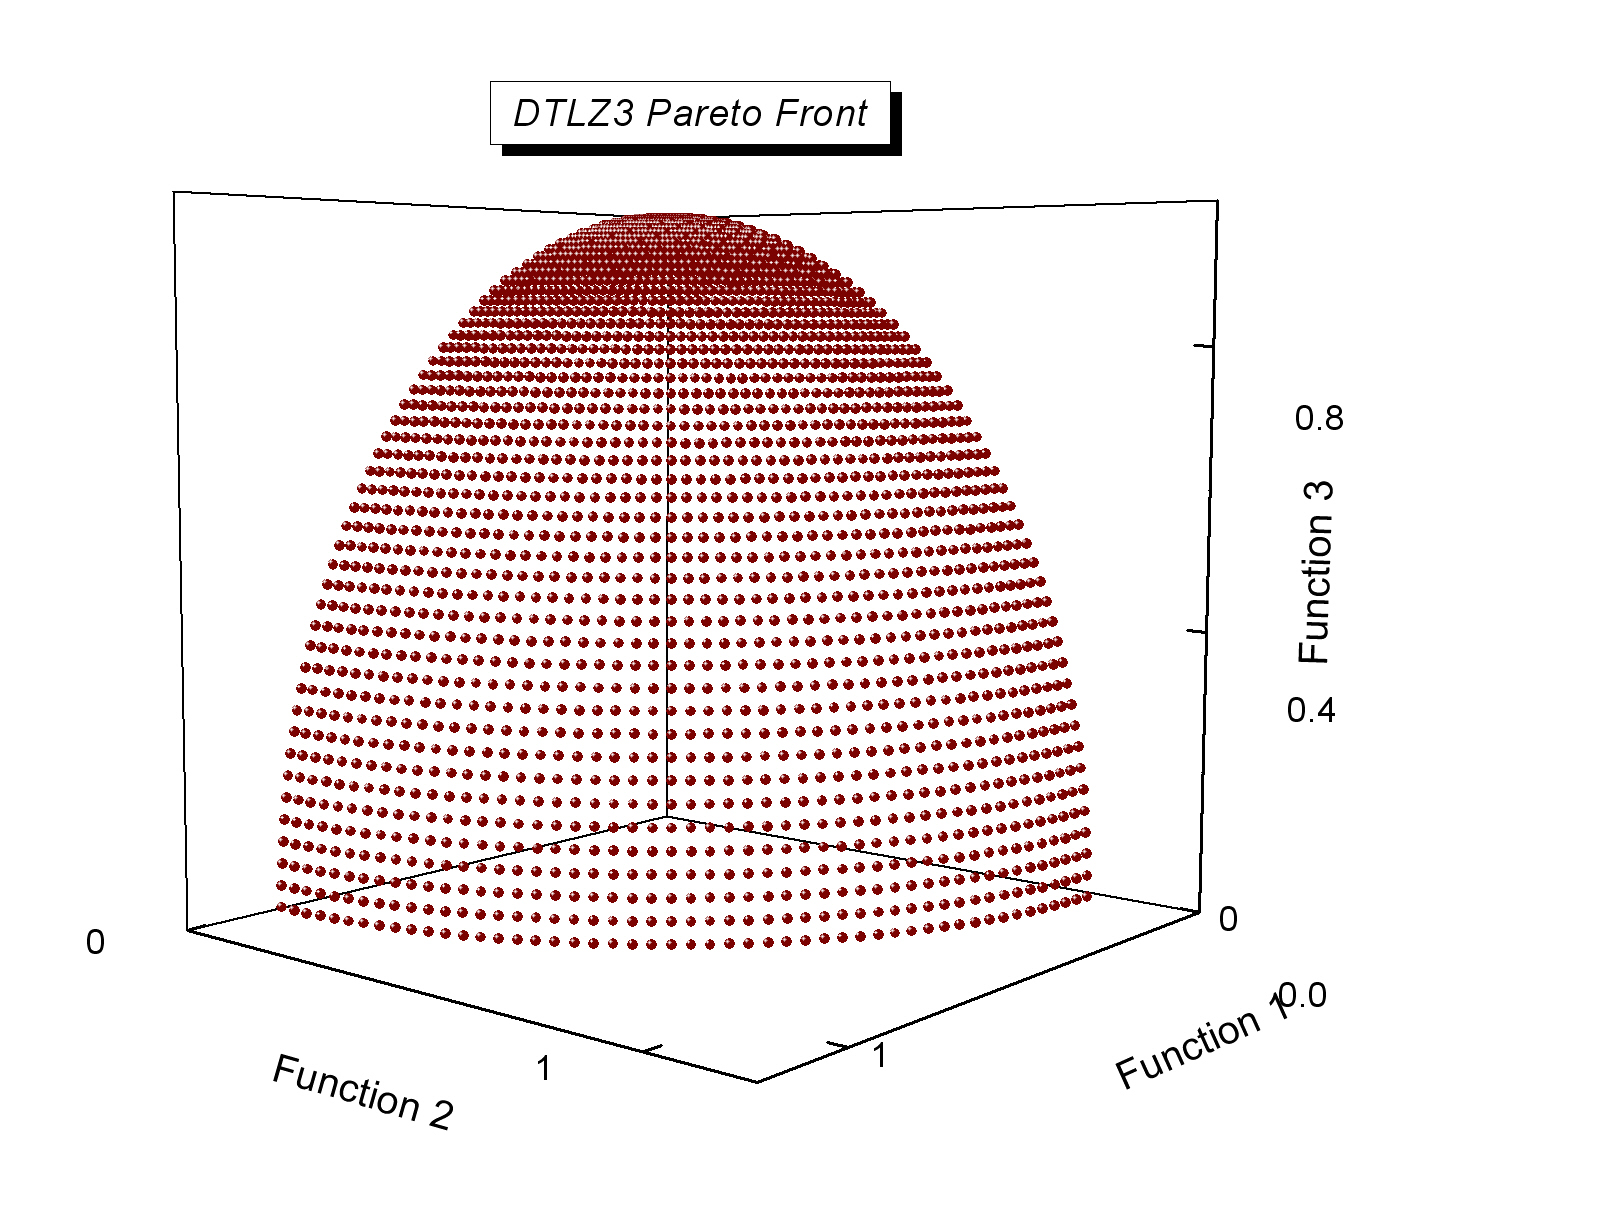
\includegraphics[scale=0.2]
{Figures_Chapter2/DTLZ3.jpg}
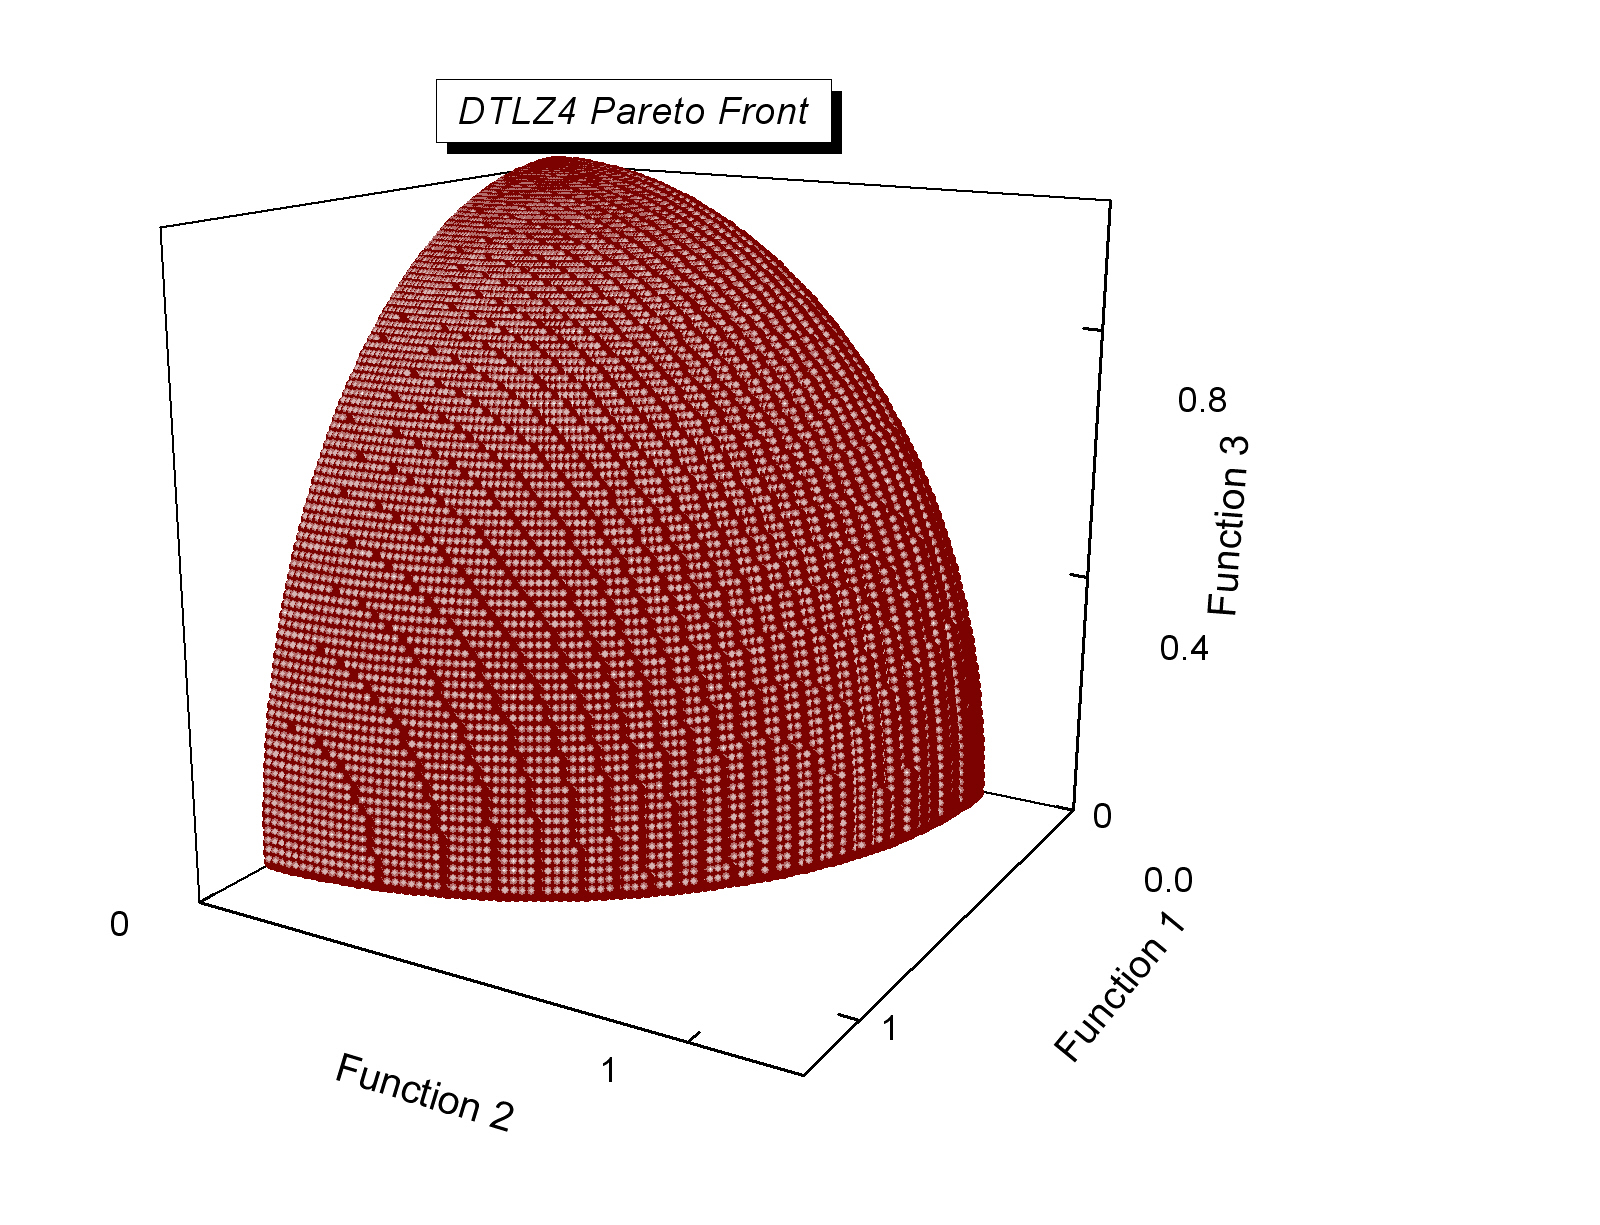
\includegraphics[scale=0.2]
{Figures_Chapter2/DTLZ4.jpg}\\
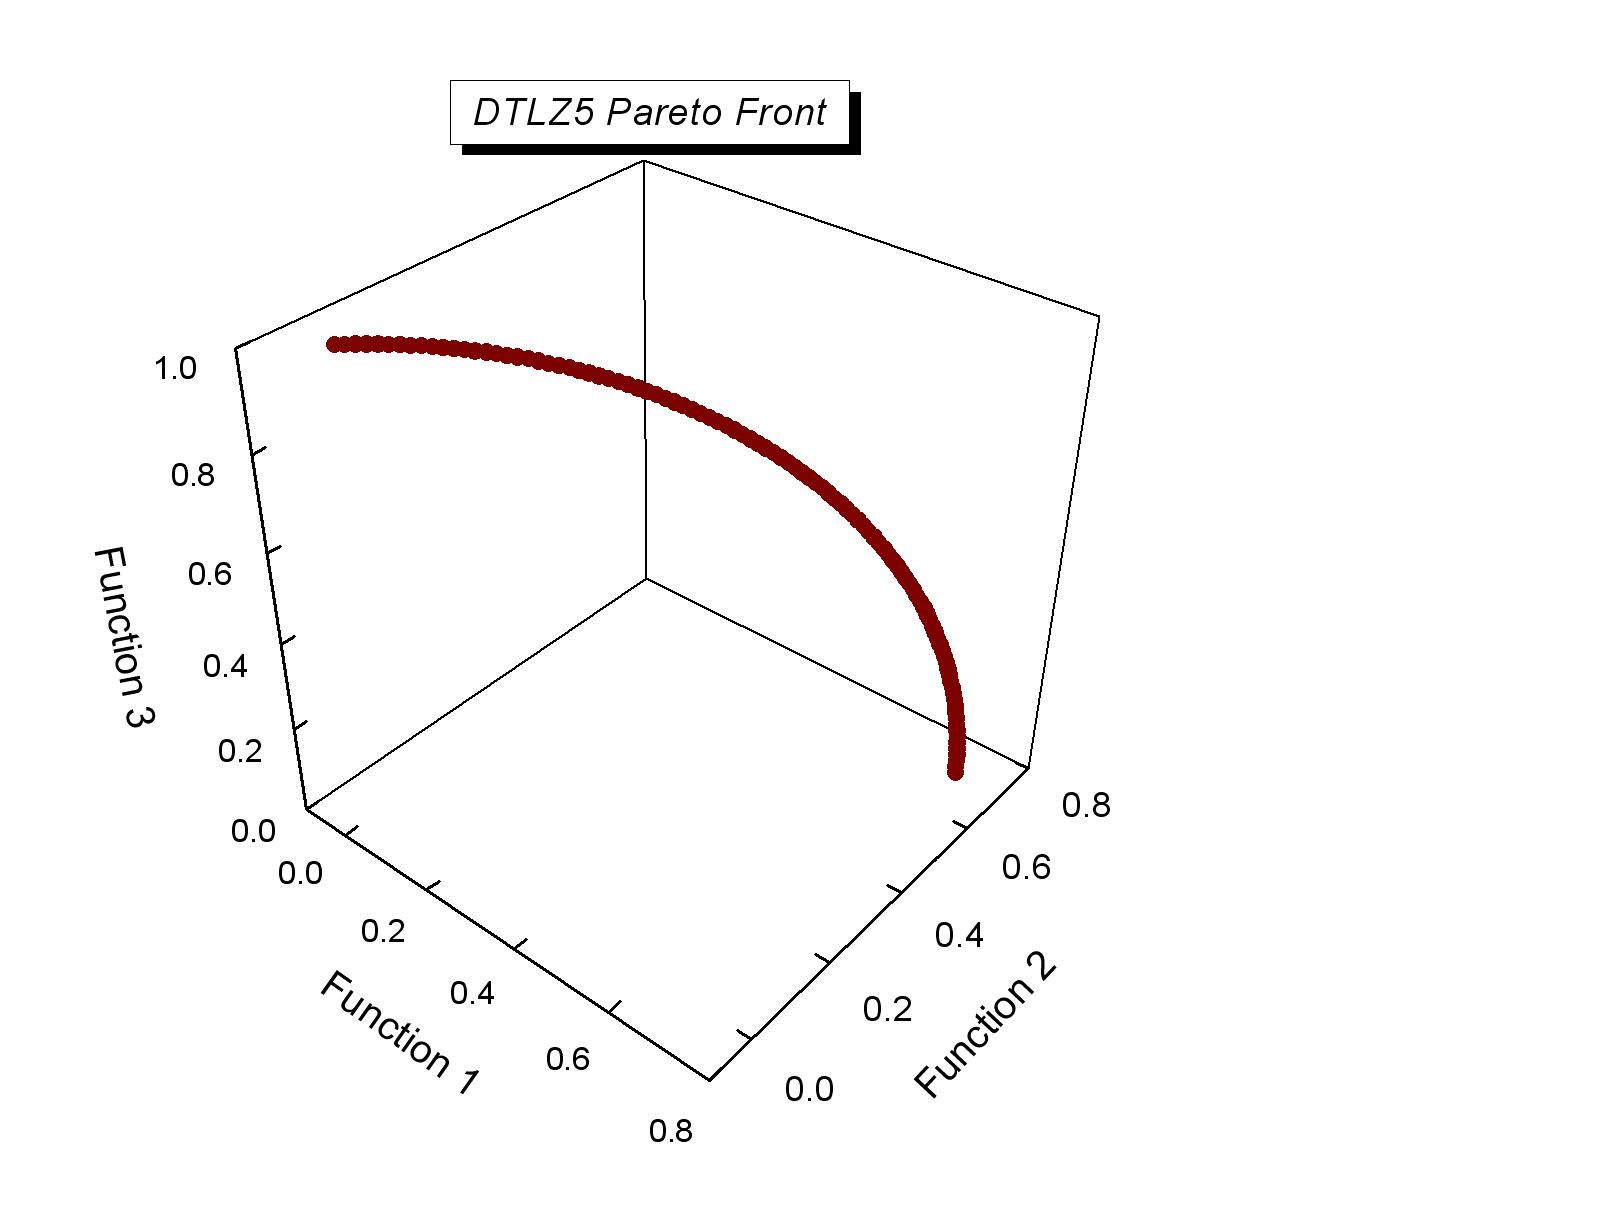
\includegraphics[scale=0.2]
{Figures_Chapter2/DTLZ5.jpg}
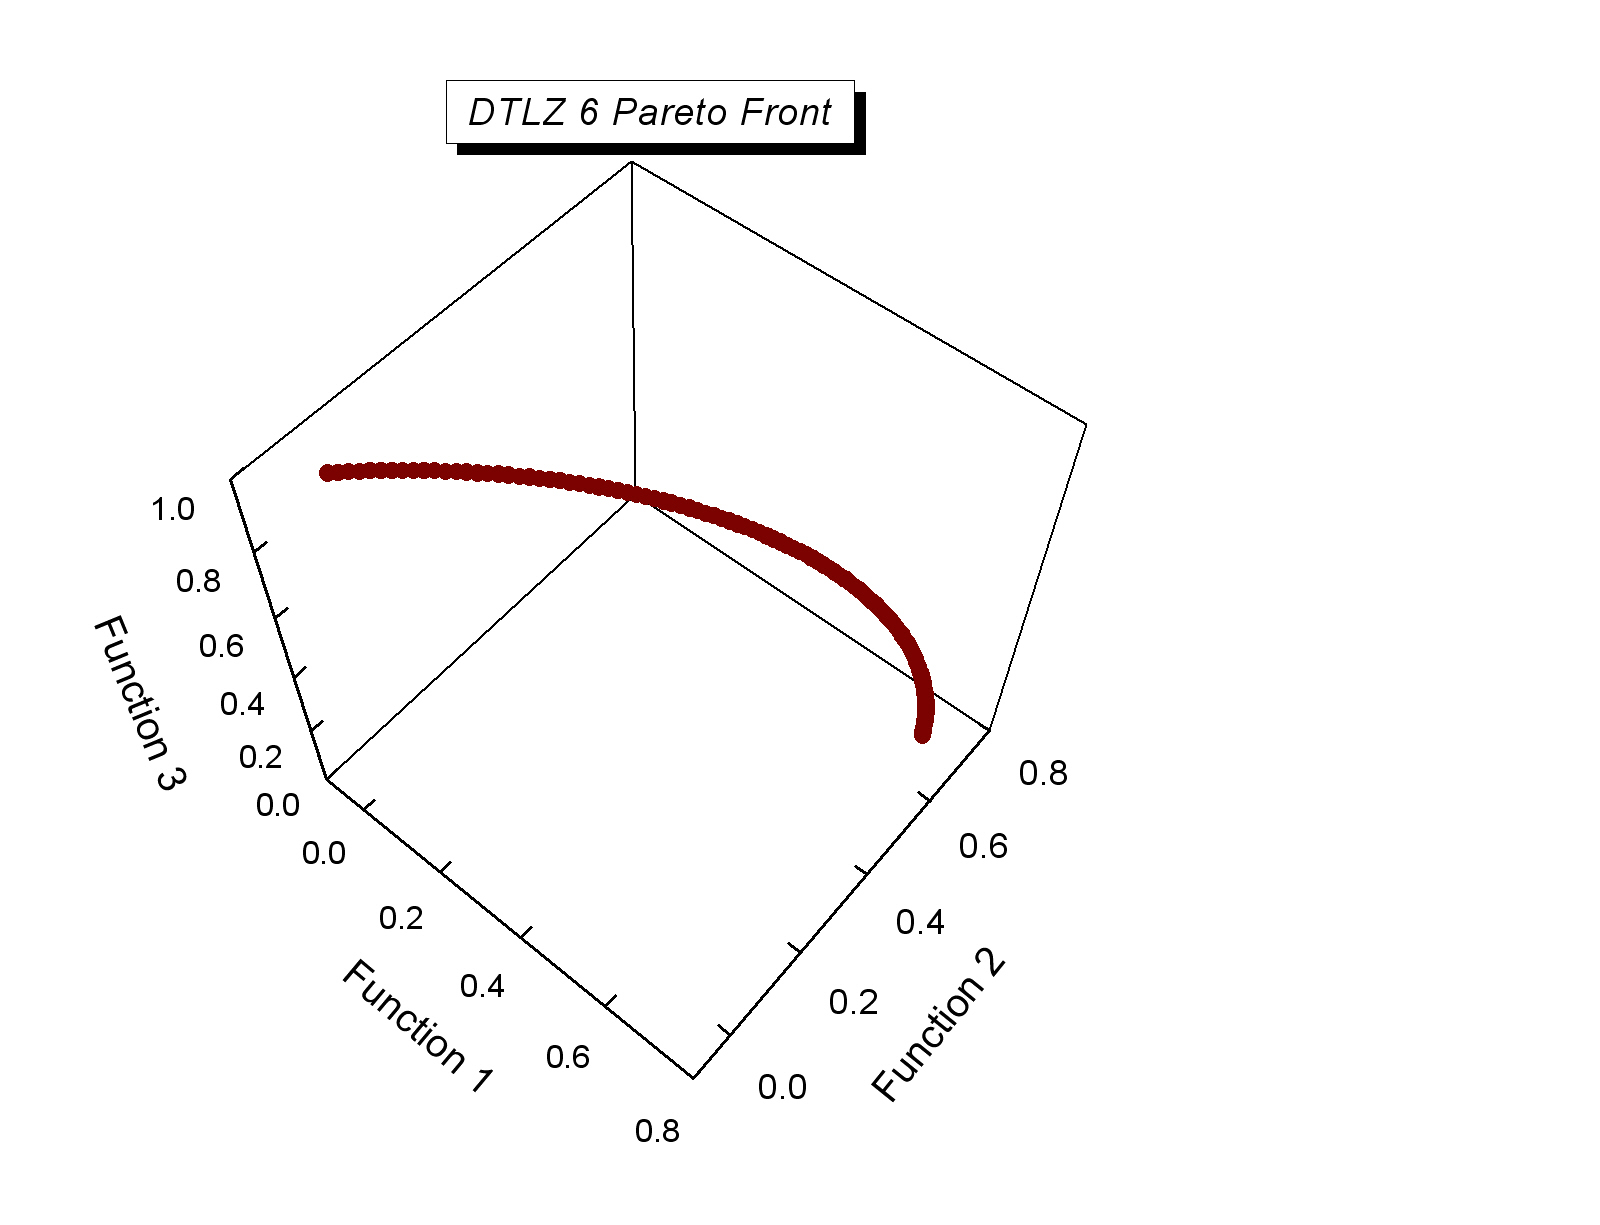
\includegraphics[scale=0.2]
{Figures_Chapter2/DTLZ6.jpg}\
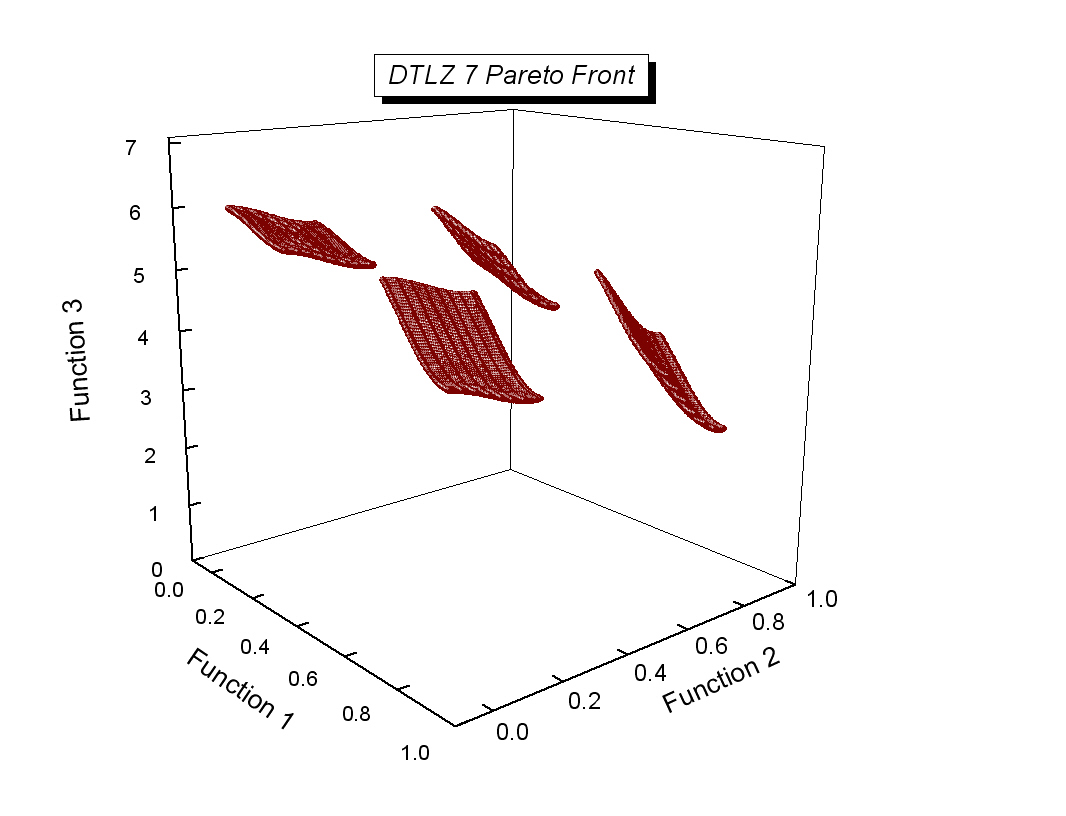
\includegraphics[scale=0.2]
{Figures_Chapter2/DTLZ7.jpg}
\end{figure}

% Please add the following required packages to your document preamble:
% \usepackage{graphicx}
\begin{table}[H]
\centering
\caption{Problemas DTLZ}
\label{tab:DTLZ}
\resizebox{\textwidth}{!}{%
\begin{tabular}{|c|l|c|}
\hline
Nombre & \multicolumn{1}{c|}{Problema} & Dominio de los parámetros \\ \hline
DTLZ1 & $ \begin{array}{lll}  f_1 &= (1+g) 0.5 \prod_{i=1}^{M-1} x_i \\ f_{m=2:M-1} &= (1+g) 0.5 (\prod_{i=1}^{M-m} x_i)(1 - y_{M-m+1}) \\ f_M &= (1+g) 0.5 (1-x_1) \\ g &= 100[x_M+\sum_{x_i \in x_M} (  (x_i - 0.5)^2 - cos(20 \pi (x_i - 0.5)) )] \end{array}$ & $[0,1]$ \\ \hline
DTLZ2 & $ \begin{array}{lll}   f_1 &= (1+g) \prod_{i=1}^{M-1} cos(x_i \pi/2) \\   f_{m=2:M-1} &= (1+g) \left (  \prod_{i=1}^{M-m} cos(x_i \pi / 2)   \right ) sin(x_{M-m+1} \pi / 2)   \\   f_M &= (1+g) sin(x_1 \pi /2) \\   g &= \sum_{x_i \in x_M} (x_i -0.5)^2 \end{array}$ & $[0,1]$ \\ \hline
DTLZ3 & Igual que DTLZ2, excepto que se utiliza la ecuación $g$ del DTLZ1 & $[0,1]$ \\ \hline
DTLZ4 & Igual que DTLZ2, excepto que $x_i \in x$ es reemplazado por $x_i ^ \alpha$, donde $\alpha > 0$ & $[0,1]$ \\ \hline
DTLZ5 & Igual que DTLZ2, excepto que $x_2, ..., x_{M-1} \in x $ son reemplazados por $\frac{1+2 g x_i}{2(1+g)}$ & $[0,1]$ \\ \hline
DTLZ6 & Igual que DTLZ5, excepto que la ecuación para $g$ es reemplazada por $g = \sum_{x_i \in x_M} x_i^{0.1}$ & $[0,1]$ \\ \hline
DTLZ7 & $ \begin{array}{lll} f_{m=1:M-1} &= x_m \\ f_M &= (1+g) \left (  M - \sum_{i=1}^{M-1} \left [ \frac{f_i}{1+g}(1 + sin(3 \pi f_i)) \right ] \right) \\ g &= 1+9 \sum_{x_i \in x_M} x_i /k \end{array}$ & $[0,1]$ \\ \hline
\end{tabular}%
}
\end{table}

\subsection{The Walking Fish Group (WFG)}
El toolkit WFG fue propuesto por \citeauthor{Joel:WFG_Main} en \citeyear{Joel:WFG_Main}, y provee las reglas para diseñar problemas personalizados, aunque en este trabajo se propusieron nueve instancias de ejemplo, éstas son utilizadas popularmente en el ámbito multi-objetivo.
%
Los problemas WFG dividen el espacio de las variables de decisión en dos subespacios: los parámetros de distancia y los parámetros de posición.
%
Un parámetro de distancia es aquel que al ser modificado siempre domina, es dominado o es un vector de parámetros equivalente.
%
Un parámetro de posición es aquel que cuando es modificado siempre resulta en un vector incomparable o un vector de parámetros equivalentes como se muestra en la figura \ref{fig:ParametrosWFG}.
%

Los nueve problemas de prueba propuestos emplean un número de funciones de transformación que facilitan la creación de vectores de transición, para dar al lector un panorama general se muestran las transiciones de cada problema de ejemplo en la tabla \ref{tab:WFG}, sin embargo no se presenta el gráfico de los frentes de Pareto debido a que sus respectivas formas están definidas por la configuración de los $l$ parámetros de distancia y los $k$ parámetros de posición, no obstante se pueden observar sus propiedades en la tabla \ref{tab:Propiedades}.
%
\subsubsection*{Observaciones WFG}
La instancia WFG1 distorsiona la importancia de cada parámetro por medio de distintos pesos mediante una reducción con suma de pesos, únicamente las instancias WFG1 y WFG7 son separables y unimodales, por otro lado la propiedad de no separabilidad de las instancias WFG6 y WFG9 provoca más dificultad en comparación a las instancias WFG2 y WFG3, la multimodalidad del WFG4 posee regiones óptimas más pronunciadas siendo más difícil que la multimodalidad de la instancia WFG9.
%
La deceptividad de la instancia WFG5 es más difícil que la instancia WFG9 ya que esta última sólo es deceptiva en los parámetros de posición.
%
Los parámetros de distancia de la instancia WFG8 son dependientes a los parámetros de posición (y entre los mismos parámetros de distancia) conformando un problema no separable.
%
Entonces en base a sus características, las instancias que se pueden considerar más difíciles son WFG5, WFG6, WFG8 y WFG9 a causa de su deceptividad, multimodalidad y dependencia.
%

Para las instancias WFG1-WFG7 una solución es óptimo de Pareto si todos los parámetros de distancia  $z_{i=k+1:n} = 2 i \times 0.35 $, particularmente el problems WFG2 es desconectado.
%
Para el problema WFG8 una solución es óptimo de Pareto si:
\begin{equation*}
\scriptsize
\begin{split}
z_{i=k+1:n} &= 2 i \times 0.35^{ \left  (   0.02 + 49.98  \left ( \frac{0.98}{49.98} - (1-2u) \left | \lfloor 0.5 - u \rfloor + \frac{0.98}{49.98} \right 	| \right  )            \right   )^{-1}    } \\
u &= r\_sum( \{ z_1, ..., z_{i-1} \}, \{ 1, ..., 1 \})
\end{split}
\end{equation*}  
Para el problema WFG9 una solución es óptimo de Pareto si:
\begin{equation*}
\scriptsize
\begin{split}
z_{i=k+1:n} &= 2 i  \begin{cases}\times 0.35^{  (0.02 + 1.96 u   )^{-1}    } & si \quad i \neq n \\ 0.35 & si \quad i=n \end{cases} \\
u &= r\_sum( \{ z_1, ..., z_{i-1} \}, \{ 1, ..., 1 \})
\end{split}
\end{equation*}

\begin{figure}[H]
\centering
\scriptsize
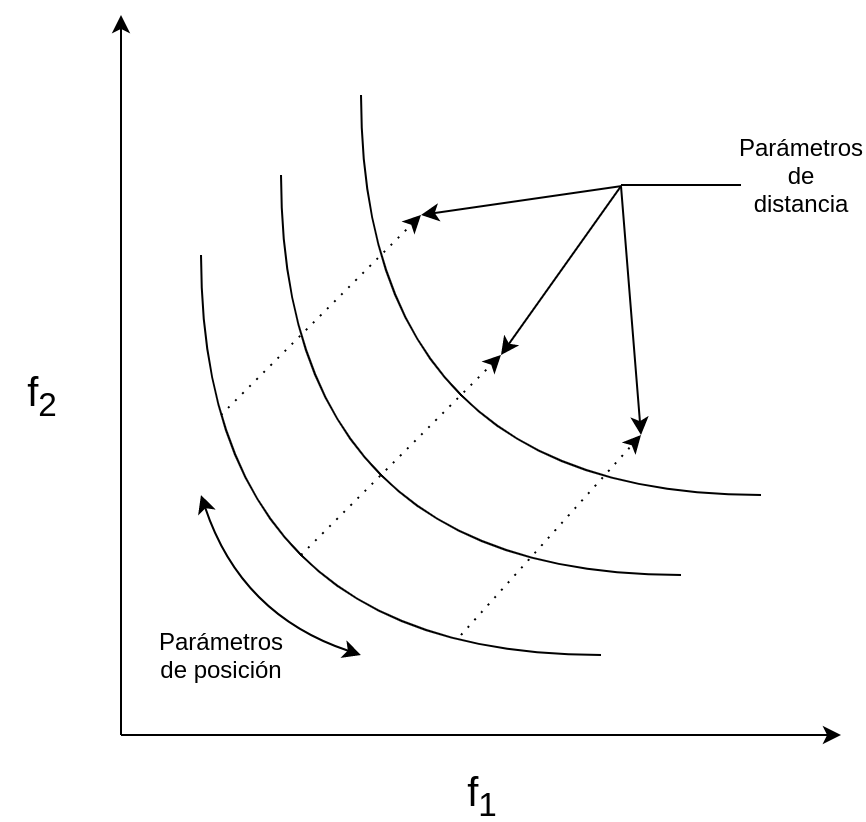
\includegraphics[scale=0.30]
{Figures_Chapter2/Parametros_Posicion_Distancia.png}
\caption{Par\'ametros de posici\'on y distancia de los problemas WFG}
\label{fig:ParametrosWFG}
\end{figure}



% Please add the following required packages to your document preamble:
% \usepackage{graphicx}
\begin{table}[]
\centering
\caption{Problemas de prueba WFG}
\label{tab:WFG}
\resizebox{\textwidth}{!}{%
\begin{tabular}{|l|l|c|}
\hline
\multicolumn{1}{|c|}{Nombre} & \multicolumn{1}{c|}{Problema} & Dominio de los parámetros \\ \hline
WFG1 & \begin{tabular}[c]{@{}l@{}}$\begin{array}{lll}      t^1_{i=1:k} &= x_i \\ t^1_{k+1:n} &= s\_linear(x_i, 0,35) \\ t^2_{i=1:k} &= x_i \\ t^2_{i=k+1:n} &= b\_flat(x_i, 0.8, 0.75, 0.85) \\ t^3_{i=1:n} &= b\_poly(x_i, 0.02) \\ t^4_{i=1:M-1} &= r\_sum(  \{ x_{(i-1)k/(M-1)+1},...,y_{ik/(M-1)} \}, \\  &\{ 2((i-1)k/(M-1)+1), ..., 2ik/(M-1) \} ) \\ t^4_M &= r\_sum( \{x_{k+1},...,y_n\}, \{ 2(k+1), ..., 2n \}) \\ h_{m=1:M-1} &= convex_m\\ \end{array}$\end{tabular} & $[0, 2 i]$ \\ \hline
WFG2 & \begin{tabular}[c]{@{}l@{}}Implementar $t^1$ del WFG1\\ $ \begin{array}{lll} t^2_{i=1:k}  &= x_i\\    t^2_{i =k+1:k+l/2} &= r\_nonsep(\{ x_{k+2(i-k)-1}, z_{k+2(i-k)}  \}, 2 )\\    t^3_{i=1:M-1} &= r\_sum( \{  x_{(i-1)k / (M-1) +1}, ..., x_{ik / (M-1)}  \}, \{1,...,1\} )\\    t^3_M &= r\_sum( \{ y_{k+1},..., y_{k+l/2}  \},\{1,...,1\} )\\    h_{m=1:M-1} &= convex_m\\    h_M &= disc_M ( \alpha = \beta =1, A = 5)\\  \end{array}$\end{tabular} & $[0, 2 i]$ \\ \hline
WFG3 & \begin{tabular}[c]{@{}l@{}}Implementar $t^1$, $t^2$ y $t^3$ del WFG2\\ $h_{m=1:M} = linear_m$\end{tabular} & $[0, 2 i]$ \\ \hline
WFG4 & \begin{tabular}[c]{@{}l@{}}$\begin{array}{lll}  t^1_{i=1:n} &= s\_multi(x_i, 30, 10, 0.35)\\   t^2_{i=1:M-1} &= r\_sum(\{ x_{(i-1)k / (M-1)+1},..., x_{ik / (M-1)}  \}, \{1,...,1\})\\   t^2_M &= r\_sum( \{ x_{k+1}, ..., x_n  \}, \{1,...,1\})\\   h_{m=1:M} &= concave_m\\ \end{array}$\end{tabular} & $[0, 2 i]$ \\ \hline
WFG5 & \begin{tabular}[c]{@{}l@{}}$t^1_{i=1:n} = s\_decept(x_i, 0.35, 0.001, 0.05)$\\ Implementar $t^2$ del WFG4 \\ $h_{m=1:M} = concave_m$\end{tabular} & $[0, 2 i]$ \\ \hline
WFG6 & \begin{tabular}[c]{@{}l@{}}Implementar $t^1$ del WFG1\\ $\begin{array}{lll} t^2_{i=1:M-1} &= r\_nonsep(\{y_{(i-1)k / (M-1) +1}, ..., y_{ik / (M-1)}\}, k/(M-1))\\  t^2_M &= r\_nonsep(\{ y_{k+1}, ..., y_n \}, l)\\ h_{m=1:M} &=concave_m\\  \end{array}$\end{tabular} & $[0, 2 i]$ \\ \hline
WFG7 & \begin{tabular}[c]{@{}l@{}}$\begin{array}{lll} t^1_{i=1:k} &= b\_param(x_i, r\_sum(\{ x_{i+1}, ..., x_n \},\{1,...,1\}), \frac{0.98}{49.88}, 0.02, 50)\\    t^1_{i=k+1:n} &=x_i\\    \end{array}$\\ Implementar $t^1$ del WFG1\\ Implementar $t^2$ del WFG4\\ $h_{m=1:M} = concave_m$\end{tabular} & $[0, 2 i]$ \\ \hline
WFG8 & \begin{tabular}[c]{@{}l@{}}$\begin{array}{lll}   t^1_{i=1:k} &= x_i\\    t^1_{k+1:n} &= b\_param( x_i, r\_sum( \{ x_1,, ...., x_{i-1} \}, \{ 1,..., 1\} ) , \frac{0.98}{49.98}, 0.02, 50)\\   \end{array}$\\ Implementar $t^2$ del WFG1\\ Implementar $t^2$ del WFG4\\ $h_{m=1:M} = concave_m$\end{tabular} & $[0, 2 i]$ \\ \hline
WFG9 & \begin{tabular}[c]{@{}l@{}}$\begin{array}{lll}t^1_{i=1:n-1} &= b\_param( x_i, r\_sum(  \{ y_{i+1}, ..., y_n \}, \{1,...,1\} ), \frac{0.98}{49.98}, 0.02, 50 )\\ t^1_{n} &= x_n\\ t^2_{i=1:k} &= s\_decept(x_i, 0.35, 0.001, 0.05)\\ t^2_{i=k+1:n} &= s\_multi(x_i, 30, 95, 0.35)\\ \end{array}$\\ Implementar $t^2$ del WFG6\\ $h_{m=1:M} = concave_m$\end{tabular} & $[0, 2 i]$ \\ \hline
\end{tabular}%
}
\end{table}

\subsection{Problemas de prueba sin restricciones (UF)}
Aunque los problemas ZDT, DTLZ y WFG, son muy implementados en el ámbito multi-objetivo, se ha propuesto un nuevo conjunto de problemas en el Congreso de Computo Evolutivo 2009 (Congress on Evolutionary Computation - CEC2009) por \cite{Joel:CEC2009}, denominados como UF (Unconstrained Functions) las cuales están compuestos por 10 problemas, donde los primeros 7 son específicamente para minimización dos objetivos y el resto de instancias son para minimización de tres objetivos. 
%

% Please add the following required packages to your document preamble:
% \usepackage{graphicx}
\begin{table}[]
\centering
\caption{Expresión del frente de Pareto y el conjunto de Pareto de los problemas UF}
\label{tab:Optimos_UF}
\resizebox{\textwidth}{!}{%
\begin{tabular}{|c|c|c|c|}
\hline
Nombre & Frente de Pareto & Conjunto de Pareto & Variables Recomendadas \\ \hline
UF1 & \begin{tabular}[c]{@{}c@{}}$f_2= 1 - \sqrt{f_1}$\\  $0 \leq f_1 \leq 1$\end{tabular} & \begin{tabular}[c]{@{}c@{}}$x_j = sin(6 \pi x_1 + \frac{j \pi}{n})$\\  $ j=2,...,n $\\ $0 \leq x_1 \leq 1$\end{tabular} & 30 \\ \hline
UF2 & \begin{tabular}[c]{@{}c@{}}$f_2= 1 - \sqrt{f_1}$\\  $0 \leq f_1 \leq 1$\end{tabular} & $ x_j =\begin{cases} \{ 0.3x_1^2 cos(24 \pi x_1 + \frac{4 j \pi}{n}) + 0.6 x_1 \} \times \\cos( 6 \pi x_1 + \frac{j \pi}{n}) \\ j \in J_1 \\ \{ 0.3x_1^2 cos(24 \pi x_1 + \frac{4 j \pi}{n}) + 0.6 x_1 \}\times \\ cos( 6 \pi x_1 + \frac{j \pi}{n}) \\ j \in J_2,\end{cases} $ & 30 \\ \hline
UF3 & \begin{tabular}[c]{@{}c@{}}$f_2 = 1 - \sqrt{f_1}$\\  $0 \leq f_1 \leq 1$\end{tabular} & \begin{tabular}[c]{@{}c@{}}$x_j = x_1^{ 0.5(1.0 + \frac{3(j-2)}{n-2}) }$\\   $j=2, ..., n, \quad 0 \leq x_1 \leq 1$\end{tabular} & 30 \\ \hline
UF4 & \begin{tabular}[c]{@{}c@{}}$f_2= 1 - f_1^2$\\  $0 \leq f_1 \leq 1$\end{tabular} & \begin{tabular}[c]{@{}c@{}}$x_j = sin(6 \pi x_1 + \frac{j \pi}{n})$\\  $j=2,...,n, \quad 0 \leq x_1 \leq 1$\end{tabular} & 30 \\ \hline
UF5 & \begin{tabular}[c]{@{}c@{}}$(\frac{i}{2N}, 1 - \frac{i}{2N}) \quad \forall i = 0,1,..., 2N$\\ \\ $N=10$, $\epsilon = 0.1$ y $n = 30$.\end{tabular} &  & 30 \\ \hline
UF6 & \begin{tabular}[c]{@{}c@{}}Consiste de un punto aislado en (0,1) y $N$ partes desconectadas\\ $f_2= 1 - f_1, f_1 \in \bigcup\limits_{i=1}^{N} [ \frac{2i - 1}{2N}$\\ $\frac{2i}{2N}]$\end{tabular} &  & 30 \\ \hline
UF7 & \begin{tabular}[c]{@{}c@{}}$f_2= 1 - f_1$\\  $0 \leq f_1 \leq 1$\end{tabular} & \begin{tabular}[c]{@{}c@{}}$x_j = sin(6 \pi x_1 + \frac{j \pi}{n})$\\ $j=2,...,n$\\ $0 \leq x_1 \leq 1$\end{tabular} & 30 \\ \hline
UF8 & \begin{tabular}[c]{@{}c@{}}$f_1^2 + f_2^2 + f_3^2 = 1$\\ $0 \leq f_1, f_2, f_3 \leq 1$\end{tabular} & \begin{tabular}[c]{@{}c@{}}$x_j = 2 x_2 sin(2 \pi x_1 + \frac{j \pi}{n})$\\ $j=3,...,n $\end{tabular} & 30 \\ \hline
UF9 & \begin{tabular}[c]{@{}c@{}}La primer parte es \\ $0 \leq f_3 \leq 1$\\ \\  $0 \leq f_1 \leq \frac{1}{4} (1 - f_3)$\\ \\ $f_2 = 1 - f_1 - f_3$\\ \\ La segunda parte es \\ $0 \leq f_3 \leq 1$, \\ \\ $\frac{3}{4} (1 - f_3) \leq f_1 \leq 1,$\\ \\ $f_2 = 1 - f_1 - f_3$\end{tabular} & \begin{tabular}[c]{@{}c@{}}Tiene dos partes desconectadas\\ $x_1 \in [0, 0.25] \cup [0.75, 1] \quad 0 \leq x_2 \leq 1$\\ \\ $x_j = 2 x_2 sin(2 \pi x_1 + \frac{j \pi}{n}), \quad j=3,...,n$\end{tabular} & 30 \\ \hline
UF10 & \begin{tabular}[c]{@{}c@{}}$f_1^2 + f_2^2 + f_3^2 = 1$ \\ $ 0 \leq f_1, f_2, f_3 \leq 1$\end{tabular} & $x_j = 2 x_2 sin (2 \pi x_1 + \frac{j \pi}{n}), \quad j=3,...,n$ & 30 \\ \hline
\end{tabular}%
}
\end{table}


%\subsubsection*{Función de prueba UF1}
%\begin{equation*}
%\scriptsize
%\begin{split}
%& minimizar \quad f_1= x_1 + \frac{2}{|J_1|} \sum_{j \in J_1} [x_j - sin(6 \pi x_1 + \frac{j \pi}{n})]^2 \\
%& minimizar \quad f_2 = 1 - \sqrt{x_1} + \frac{1}{|J_2|} \sum_{j \in J_2} [x_j - sin( 6 \pi x_1 + \frac{j \pi}{n}]^2
%\end{split}
%\end{equation*}
% Donde
% $J_1 = \{ j|j$ es impar y $2 \leq j \leq n \}$ y $J_2 = \{ j|j$ es par con $2 \leq j \leq n \}$, el espacio de búsqueda esta comprendido por $[0, 1] \times [-1,1]^{n-1}$.
 %
 
% El frente de Pareo óptimo es:
% \begin{equation*}
% f_2= 1 - \sqrt{f_1}, \quad 0 \leq f_1 \leq 1
% \end{equation*}
% %
% 
% El conjunto de Pareto está definido por:
% \begin{equation*}
%x_j = sin(6 \pi x_1 + \frac{j \pi}{n}), \quad j=2,...,n, \quad 0 \leq x_1 \leq 1
% \end{equation*}
%
%El número de variables utilizadas son $n=30$.
%\begin{figure}[H]
%\centering
%\scriptsize
%\includegraphics[scale=0.5]
%{Figures_Chapter2/UF1.eps}
%%\decoRule
%\caption{Frente de Pareto y conjunto de Pareto del problema UF1}
%\label{fig:UF1}
%\end{figure}

%\subsubsection*{Función de prueba UF2}
%\begin{equation*}
%\scriptsize
%\begin{split}
%& minimizar \quad f_1= x_1 + \frac{2}{|J_1|} \sum_{j \in J_1} y_j^2 \\
%& minimizar \quad f_2 = 1 - \sqrt{x_1} + \frac{1}{|J_2|} \sum_{j \in J_2} y_j^2
%\end{split}
%\end{equation*}
% Donde
% $J_1 = \{ j|j$ es impar y $2 \leq j \leq n \}$ y $J_2 = \{ j|j$ es par con $2 \leq j \leq n \}$, el espacio de búsqueda esta comprendido por $[0, 1] \times [-1,1]^{n-1}$.
% %
% \begin{equation}
% y_j = 
% \begin{cases}
% x_j - [0.3x_1^2 cos(24 \pi x_1 + \frac{4 j \pi}{n}) + 0.6 x_1] cos( 6 \pi x_1 + \frac{j \pi}{n} \quad j \in J_1 \\
% x_j - [0.3x_1^2 cos(24 \pi x_1 + \frac{4 j \pi}{n}) + 0.6 x_1] cos( 6 \pi x_1 + \frac{j \pi}{n} \quad j \in J_2 
% \end{cases}
% \end{equation}
 %
% El frente de Pareo óptimo es:
% \begin{equation*}
% f_2= 1 - \sqrt{f_1}, \quad 0 \leq f_1 \leq 1
% \end{equation*}
% %
% 
% 
% El conjunto de Pareto es:
% \begin{equation*}
% x_j = 
% \begin{cases}
% \{ 0.3x_1^2 cos(24 \pi x_1 + \frac{4 j \pi}{n}) + 0.6 x_1 \} cos( 6 \pi x_1 + \frac{j \pi}{n} \quad j \in J_1 \\
% \{ 0.3x_1^2 cos(24 \pi x_1 + \frac{4 j \pi}{n}) + 0.6 x_1 \} cos( 6 \pi x_1 + \frac{j \pi}{n} \quad j \in J_2 
% \end{cases}
% \end{equation*}
%El número de variables utilizadas son $n=30$.
%\begin{figure}[H]
%\centering
%\scriptsize
%\includegraphics[scale=0.5]
%{Figures_Chapter2/UF2.eps}
%\caption{Frente de Pareto y conjunto de Pareto del problema UF2}
%\label{fig:UF2}
%\end{figure}


%\subsubsection*{Función de prueba UF3}
%\begin{equation*}
%\scriptsize
%\begin{split}
%& minimizar \quad f_1= x_1 + \frac{2}{|J_1|} ( 4 \sum_{j \in J_1} y_j^2 - 2 \prod_{j \in J_1} cos (  \frac{20 y_j \pi}{ \sqrt[]{j}} ) + 2 ) \\
%& minimizar \quad f_2=  1 - \sqrt[]{x_1} + \frac{2}{|J_2|} ( 4 \sum_{j \in J_2} y_j^2 - 2 \prod_{j \in J_2} cos (  \frac{20 y_j \pi}{ \sqrt[]{j}} ) + 2 ) 
%\end{split}
%\end{equation*}
% Donde
% $J_1$ y $J_2$ son iguales como en F1, el espacio de búsqueda esta comprendido por $[0, 1]^n$.
% %
% \begin{equation*}
%    y_j = x_1^{ 0.5(1.0 + \frac{3(j-2)}{n-2}) }, \quad j=2, ..., n,
%\end{equation*}
 
% El frente de Pareo óptimo es:
% \begin{equation*}
%   f_2 = 1 - \sqrt[]{f_1}, \quad 0 \leq f_1 \leq 1.
%\end{equation*}
%
% %
% El conjunto de Pareto es:
% \begin{equation*}
%	x_j = x_1^{ 0.5(1.0 + \frac{3(j-2)}{n-2}) }, \quad j=2, ..., n, \quad 0 \leq x_1 \leq 1. 
% \end{equation*}
%
%El número de variables utilizadas son $n=30$
%\begin{figure}[H]
%\centering
%\scriptsize
%\includegraphics[scale=0.5]
%{Figures_Chapter2/UF3.eps}
%\caption{Frente de Pareto y conjunto de Pareto del problema UF3}
%\label{fig:UF3}
%\end{figure}


%\subsubsection*{Función de prueba UF4}
%\begin{equation*}
%\scriptsize
%\begin{split}
%& minimizar \quad f_1= x_1 + \frac{2}{|J_1|} \sum_{j \in J_1} h(y_j)\\
%& minimizar \quad f_2= 1 - x_1^2 + \frac{2}{|J_2|} \sum_{j \in J_2} h(y_j)
%\end{split}
%\end{equation*}
% Donde
% $J_1 = \{ j|j$ es impar y $2 \leq j \leq n \}$ y $J_2 = \{ j|j$ es par con $2 \leq j \leq n \}$, el espacio de búsqueda esta comprendido por $[0, 1] \times [-2,2]^{n-1}$.
% %
% \begin{equation*}
% \begin{split}
% y_j = x_j - sin( 6 \pi x_1 + \frac{j \pi}{ n} ), j=2, ..., n. \\
% h(t) = \frac{|t|}{ 1 ++ e^{2 |t| }}
% \end{split}
% \end{equation*}
 
% El frente de Pareo óptimo es:
% \begin{equation*}
% f_2= 1 - f_1^2, \quad 0 \leq f_1 \leq 1
% \end{equation*}
%
% %
% El conjunto de Pareto es:
% \begin{equation*}
%x_j = sin(6 \pi x_1 + \frac{j \pi}{n}), \quad j=2,...,n, \quad 0 \leq x_1 \leq 1
% \end{equation*}
%
%El número de variables utilizadas son $n=30$

%\begin{figure}[H]
%\centering
%\scriptsize
%\includegraphics[scale=0.5]
%{Figures_Chapter2/UF4.eps}
%\caption{Frente de Pareto y conjunto de Pareto del problema UF4}
%\label{fig:UF4}
%\end{figure}

%\subsubsection*{Función de prueba UF5}
%\begin{equation*}
%\scriptsize
%\begin{split}
%& minimizar \quad f_1= x_1 +  (\frac{1}{2N} + \epsilon) | sin(2 N \pi x_1)  +\frac{2}{|J_1|} \sum_{j \in J_1} h(y_j)\\
%& minimizar \quad f_2= 1 - x_1 +  (\frac{1}{2N} + \epsilon) | sin(2 N \pi x_1)  +\frac{2}{|J_2|} \sum_{j \in J_2} h(y_j)\\
%\end{split}
%\end{equation*}
% Donde
% $J_1 = \{ j|j$ es impar y $2 \leq j \leq n \}$ y $J_2 = \{ j|j$ es par con $2 \leq j \leq n \}$. N es un entero, $\epsilon >0$ ,el espacio de búsqueda esta comprendido por $[0, 1] \times [-1,1]^{n-1}$.
% %
% \begin{equation*}
% \begin{split}
% y_j = x_j - sin( 6 \pi x_1 + \frac{j \pi}{ n} ), j=2, ..., n. \\
% h(t) = 2t^2 - cos(4 \pi t) + 1
% \end{split}
% \end{equation*}
 
% El frente de Pareo óptimo tiene 2N + 1 soluciones:
% \begin{equation*}
%(\frac{i}{2N}, 1 - \frac{i}{2N}) \quad \forall i = 0,1,..., 2N.
% \end{equation*}
%$N=10$, $\epsilon = 0.1$ y $n = 30$.

%\begin{figure}[H]
%\centering
%\scriptsize
%\includegraphics[scale=0.5]
%{Figures_Chapter2/UF5.eps}
%\caption{Frente de Pareto y conjunto de Pareto del problema UF5}
%\label{fig:UF5}
%\end{figure}

%\subsubsection*{Función de prueba UF6}
%\begin{equation*}
%\scriptsize
%\begin{split}
%& minimizar \quad f_1= x_1 + max \{ 0,  2(\frac{1}{2N} + \epsilon ) sin(2N \pi x_1)  \} + \frac{2}{|J_1|} ( 4 \sum_{j \in J_1} y_j^2 - 2 \prod_{j \in J_1} cos( \frac{20 y_j \pi}{\sqrt[]{j}} ) + 2  )  \\
%& minimizar \quad f_2= 1 - x_1 + max \{ 0,  2(\frac{1}{2N} + \epsilon ) sin(2N \pi x_1)  \} + \frac{2}{|J_2|} ( 4 \sum_{j \in J_2} y_j^2 - 2 \prod_{j \in J_2} cos( \frac{20 y_j \pi}{\sqrt[]{j}} ) + 2  )  \\
%\end{split}
%\end{equation*}
% Donde
% $J_1 = \{ j|j$ es impar y $2 \leq j \leq n \}$ y $J_2 = \{ j|j$ es par con $2 \leq j \leq n \}$, el espacio de búsqueda esta comprendido por $[0, 1] \times [-1,1]^{n-1}$.
% %
% \begin{equation*}
% y_j= x_j - sin(6 \pi x_1 + \frac{j \pi}{n}), j=2,...,n.
% \end{equation*}
 
% El frente de Pareo óptimo consiste de un punto aislado y $N$ parte desconectadas.
% \begin{equation*}
% f_2= 1 - f_1, f_1 \in \bigcup\limits_{i=1}^{N} [ \frac{2i - 1}{2N}, \frac{2i}{2N}].
% \end{equation*}
%$N=2$, $\epsilon = 0.1$ y $n=30$.
% \begin{figure}[H]
%\centering
%\scriptsize
%\includegraphics[scale=0.5]
%{Figures_Chapter2/UF6.eps}
%\caption{Frente de Pareto y conjunto de Pareto del problema UF6}
%\label{fig:UF6}
%\end{figure}

%\subsubsection*{Función de prueba UF7}
%\begin{equation*}
%\scriptsize
%\begin{split}
%& minimizar \quad f_1= \sqrt[5]{x_1} + \frac{2}{|J_1|} \sum_{j \in J_1} y_j^2 \\
%& minimizar \quad f_2= 1 - \sqrt[5]{x_1} + \frac{2}{|J_2|} \sum_{j \in J_2} y_j^2 \\
%\end{split}
%\end{equation*}
% Donde
% $J_1 = \{ j|j$ es impar y $2 \leq j \leq n \}$ y $J_2 = \{ j|j$ es par con $2 \leq j \leq n \}$, el espacio de búsqueda esta comprendido por $[0, 1] \times [-1,1]^{n-1}$.
% %
% \begin{equation*}
% y_j = x_j - sin(6 \pi x_1 + \frac{j \pi}{n} ), j=2,..., n
% \end{equation*}
 
% El frente de Pareo óptimo es
% \begin{equation*}
% f_2= 1 - f_1, \quad 0 \leq f_1 \leq 1
% \end{equation*}
%
% %
% El conjunto de Pareto es
% \begin{equation*}
%x_j = sin(6 \pi x_1 + \frac{j \pi}{n}), \quad j=2,...,n, \quad 0 \leq x_1 \leq 1
% \end{equation*}
%
%El número de variables utilizados son $n=30$
%\begin{figure}[H]
%\centering
%\scriptsize
%\includegraphics[scale=0.5]
%{Figures_Chapter2/UF7.eps}
%\caption{Frente de Pareto y conjunto de Pareto del problema UF7}
%\label{fig:UF7}
%\end{figure}

%\subsubsection*{Función de prueba UF8}
%\begin{equation*}
%\scriptsize
%\begin{split}
%& minimizar \quad f_1= cos(0.5 x_1 \pi) cos(0.5 x_2 \pi ) + \frac{2}{J_1} \sum_{j \in J_1} (x_j - 2 x_2 sin(2\pi x_1 + \frac{j \pi}{n}))^2\\
%& minimizar \quad f_2= cos(0.5 x_1 \pi) sin(0.5 x_2 \pi ) + \frac{2}{J_2} \sum_{j \in J_1} (x_j - 2 x_2 sin(2\pi x_1 + \frac{j \pi}{n}))^2\\
%& minimizar \quad f_3= sin(0.5 x_1 \pi ) + \frac{2}{J_3} \sum_{j \in J_1} (x_j - 2 x_2 sin(2\pi x_1 + \frac{j \pi}{n}))^2
%\end{split}
%\end{equation*}
% Donde
% $J_1 = \{ j|3 \leq j \leq n \}$, y $j-1$ es una multiplicación de 3, \\
% $J_2 = \{ j|3 \leq j \leq n \}$, y $j-2$ es una multiplicación de 3, \\
% $J_3 = \{ j|3 \leq j \leq n \}$, y $j$ es una multiplicación de 3. 
% %
%El espacio de búsqueda es $[0,1]^2 \times [-2, 2]^{n-2}$

% El frente de Pareo óptimo es
% \begin{equation*}
% f_1^2 + f_2^2 + f_3^2 = 1, 0 \leq f_1, f_2, f_3 \leq 1. 
% \end{equation*}
% %
% El conjunto de Pareto es
% \begin{equation*}
%x_j = 2 x_2 sin(2 \pi x_1 + \frac{j \pi}{n}), \quad j=3,...,n.
% \end{equation*}
%
%El número de variables utilizados son $n=30$
%\begin{figure}[H]
%\centering
%\scriptsize
%\includegraphics[scale=0.5]
%{Figures_Chapter2/UF8.eps}
%\caption{Frente de Pareto y conjunto de Pareto del problema UF8}
%\label{fig:UF8}
%\end{figure}

%\subsubsection*{Función de prueba UF9}
%\begin{equation*}
%\scriptsize
%\begin{split}
%& minimizar \quad f_1= 0.5[ max\{ 0,  (1 + \epsilon) (1 - 4(2 x_1 - 1)^2 ) \} + 2 x_1] x_2 + \frac{2}{|J_1|} \sum_{j \in J_1} ( x_j - 2 x_2 sin(2 \pi x_1 + \frac{j \pi}{n}) )^2\\
%& minimizar \quad f_2= 0.5[ max\{ 0,  (1 + \epsilon) (1 - 4(2 x_1 - 1)^2 ) \} - 2 x_1 + 2] x_2 + \frac{2}{|J_2|} \sum_{j \in J_2} ( x_j - 2 x_2 sin(2 \pi x_1 + \frac{j \pi}{n}) )^2\\
%& minimizar \quad f_3= 1 - x_2 + \frac{2}{|J_3|} \sum_{j \in J_3} ( x_j - 2 x_2 sin(2 \pi x_1 + \frac{j \pi}{n}) )^2
%\end{split}
%\end{equation*}
% Donde
% $J_1 = \{ j|3 \leq j \leq n \}$, y $j-1$ es una multiplicación de 3, \\
% $J_2 = \{ j|3 \leq j \leq n \}$, y $j-2$ es una multiplicación de 3, \\
% $J_3 = \{ j|3 \leq j \leq n \}$, y $j$ es una multiplicación de 3. \\
% $\epsilon = 0.1$\\
% %
%El espacio de búsqueda es $[0,1]^2 \times [-2, 2]^{n-2}$

% El frente de Pareo óptimo tiene dos partes. La primer parte es
%\begin{equation*}
%\begin{split}
%0 \leq f_3 \leq 1, \\
%0 \leq f_1 \leq \frac{1}{4} (1 - f_3),\\
%f_2 = 1 - f_1 - f_3
%\end{split}
%\end{equation*}
% %
%La segunda parte es:
%\begin{equation*}
%\begin{split}
%0 \leq f_3 \leq 1, \\
%\frac{3}{4} (1 - f_3) \leq f_1 \leq 1,\\
%f_2 = 1 - f_1 - f_3
%\end{split}
% \end{equation*}
% 
% %
%El conjunto de Pareto, también tiene dos partes:
% \begin{equation*}
% \begin{split}
%   x_1 \in [0, 0.25] \cup [0.75, 1], \quad 0 \leq x_2 \leq 1,\\
%   x_j = 2 x_2 sin (2 \pi x_1 + \frac{j \pi}{n}), \quad j=3,...,n.
% \end{split}
% \end{equation*}
%
%El número de variables utilizados son $n=30$

%\begin{figure}[H]
%\centering
%\scriptsize
%\includegraphics[scale=0.5]
%{Figures_Chapter2/UF9.eps}
%\caption{Frente de Pareto y conjunto de Pareto del problema UF9}
%\label{fig:UF9}
%\end{figure}
%\subsubsection*{Función de prueba UF10}
%\begin{equation*}
%\scriptsize
%\begin{split}
%& minimizar \quad f_1= cos(0.5 x_1 \pi ) cos(0.5 x_2 \pi) + \frac{2}{|J_1|} \sum_{j \in J_1} [ 4 y_j^2 - cos( 8 \pi y_j) + 1] \\
%& minimizar \quad f_2= cos(0.5 x_1 \pi ) sin(0.5 x_2 \pi) + \frac{2}{|J_2|} \sum_{j \in J_2} [ 4 y_j^2 - cos( 8 \pi y_j) + 1] \\
%& minimizar \quad f_3= sin(0.5 x_1 \pi) + \frac{2}{|J_3|} \sum_{j \in J_3} [ 4 y_j^2 - cos( 8 \pi y_j) + 1]
%\end{split}
%\end{equation*}
% Donde
% $J_1 = \{ j|3 \leq j \leq n \}$, y $j-1$ es una multiplicación de 3, \\
% $J_2 = \{ j|3 \leq j \leq n \}$, y $j-2$ es una multiplicación de 3, \\
% $J_3 = \{ j|3 \leq j \leq n \}$, y $j$ es una multiplicación de 3. \\
% \begin{equation*}
%\begin{split}
%y_j = x_j - 2 x_2 sin( 2 \pi x_1 + \frac{j \pi}{n}), \quad j=3, ..., n
%\end{split}
%\end{equation*}
% %
%El espacio de búsqueda es $[0,1]^2 \times [-2, 2]^{n-2}$

% El frente de Pareo óptimo es:
%\begin{equation*}
%\begin{split}
%f_1^2 + f_2^2 + f_3^2 = 1, \quad 0 \leq f_1, f_2, f_3 \leq 1 
%\end{split}
%\end{equation*}
% %
%El conjunto de Pareto es:
% \begin{equation*}
% \begin{split}
%   x_j = 2 x_2 sin (2 \pi x_1 + \frac{j \pi}{n}), \quad j=3,...,n.
% \end{split}
% \end{equation*}
%
%El número de variables utilizados son $n=30$
%\begin{figure}[H]
%\centering
%\scriptsize
%\includegraphics[scale=0.5]
%{Figures_Chapter2/UF10.eps}
%\caption{Frente de Pareto y conjunto de Pareto del problema UF10}
%\label{fig:UF10}
%\end{figure}


% Please add the following required packages to your document preamble:
% \usepackage{graphicx}
\begin{table}[]
\centering
\caption{Frente de Pareto y conjunto óptimo de los problemas UF.}%proyección del conjunto de soluciones óptimas.}
\label{fig:Formas_UF}
\resizebox{\textwidth}{!}{%
\begin{tabular}{cc}
UF1 & UF2 \\
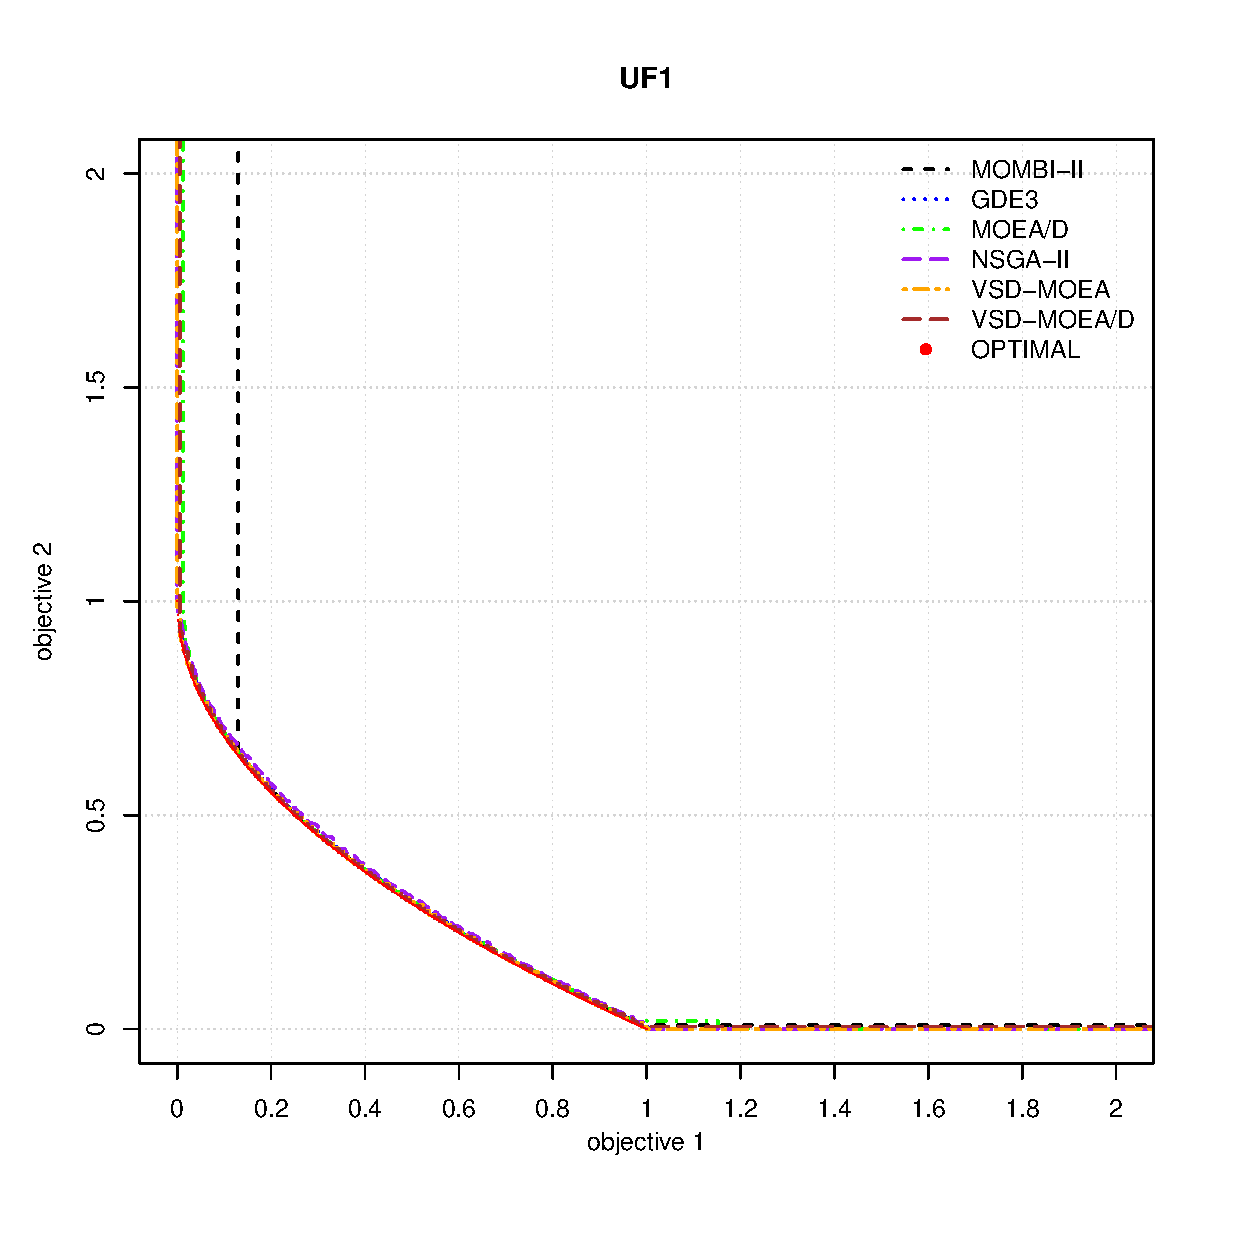
\includegraphics[scale=0.5]{Figures_Chapter2/UF1.eps} & 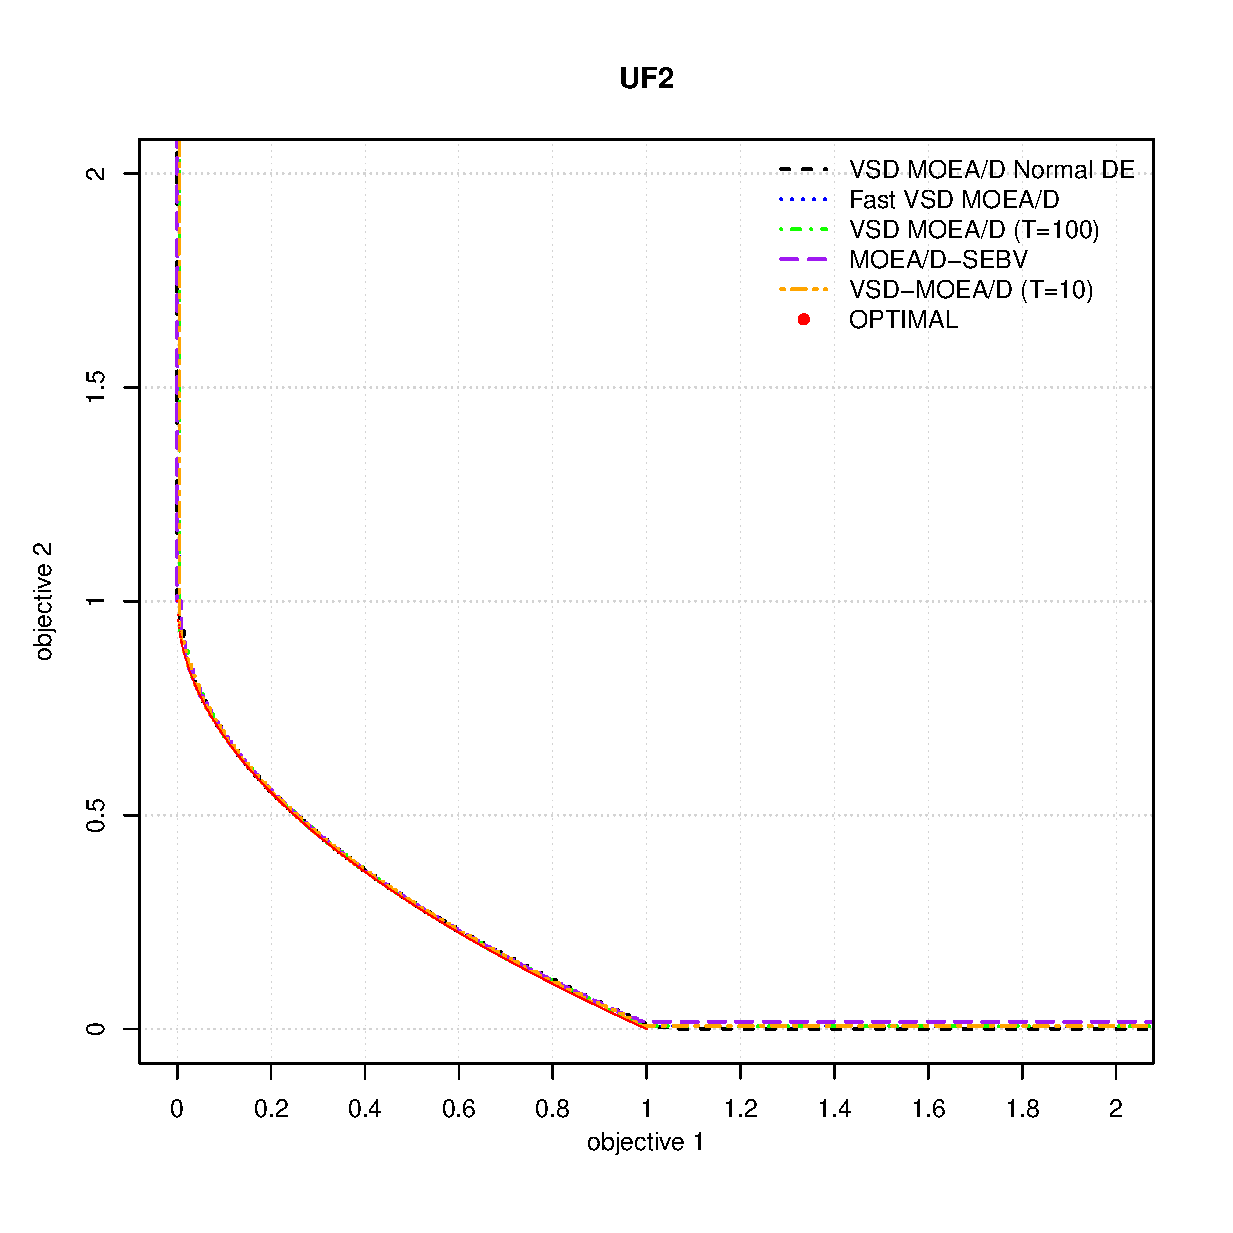
\includegraphics[scale=0.5]{Figures_Chapter2/UF2.eps} \\
UF3 & UF4 \\
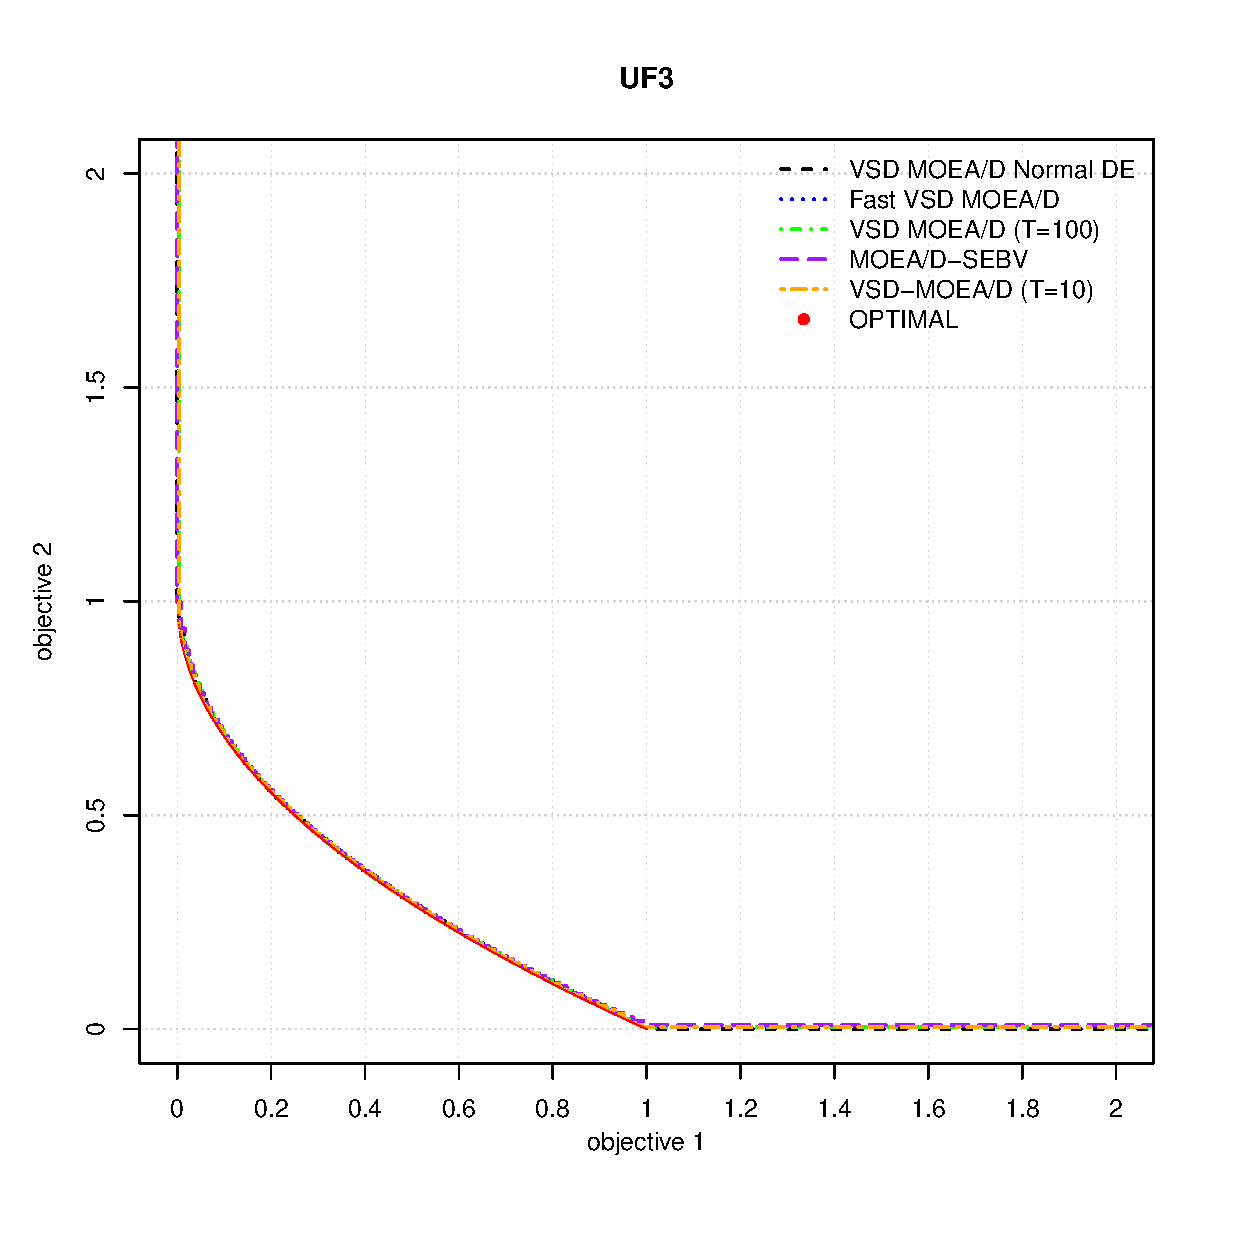
\includegraphics[scale=0.5]{Figures_Chapter2/UF3.eps} & 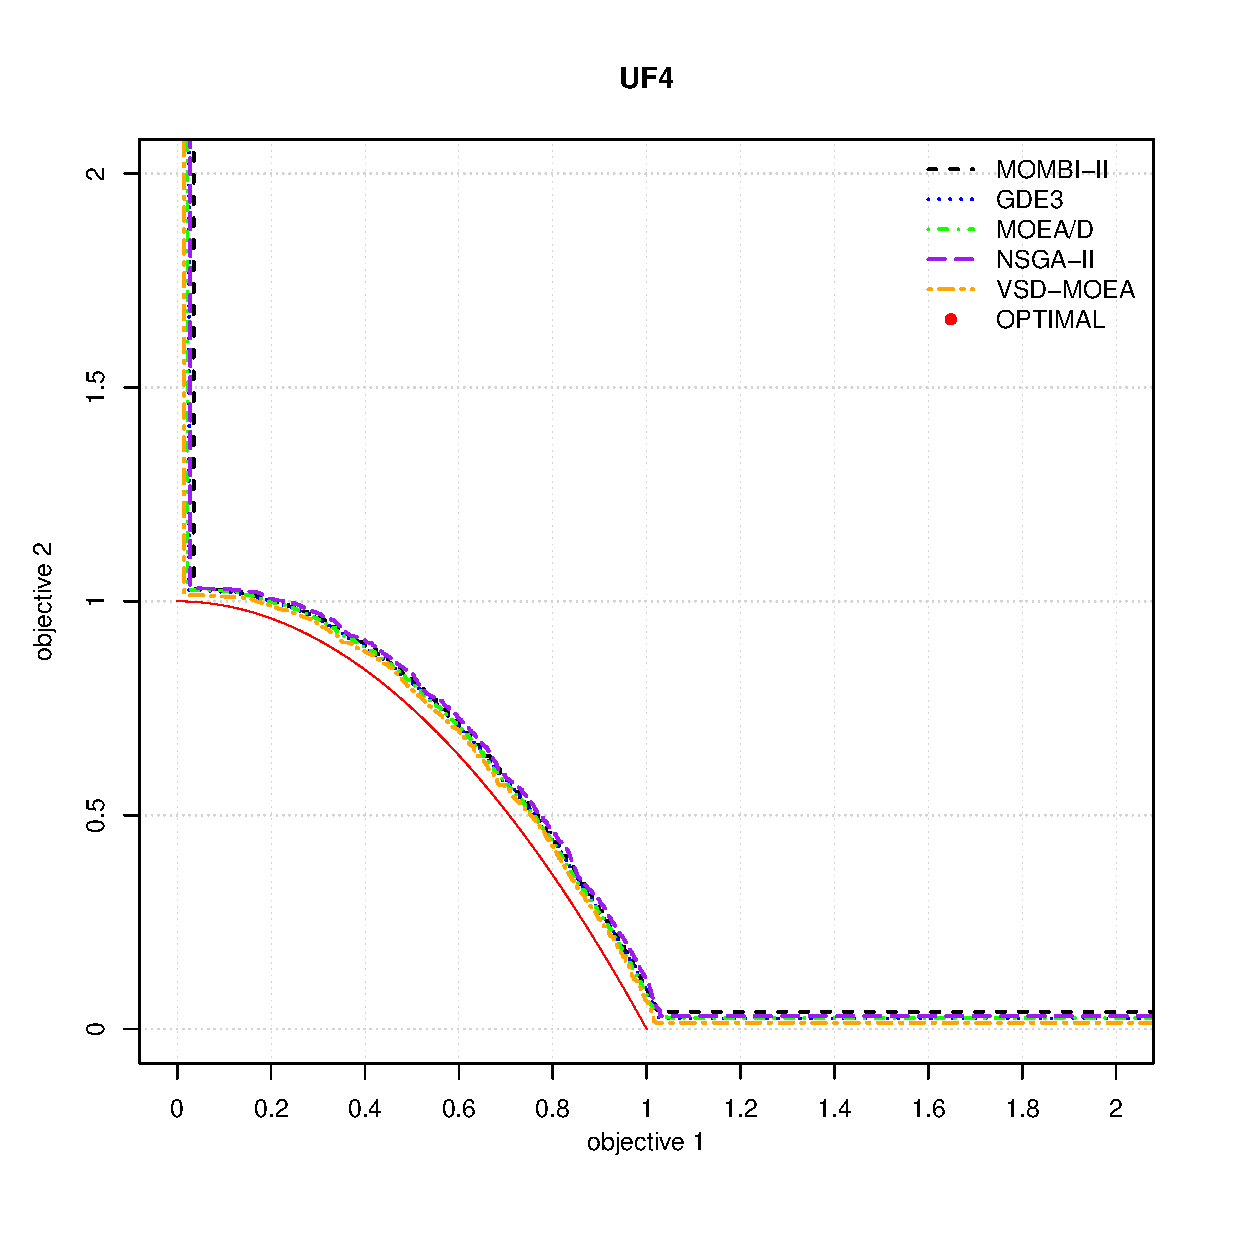
\includegraphics[scale=0.5]{Figures_Chapter2/UF4.eps} \\
UF5 & UF6 \\
\includegraphics[scale=0.5]{Figures_Chapter2/UF5.eps} & \includegraphics[scale=0.5]{Figures_Chapter2/UF6.eps} \\
UF7 & UF8 \\
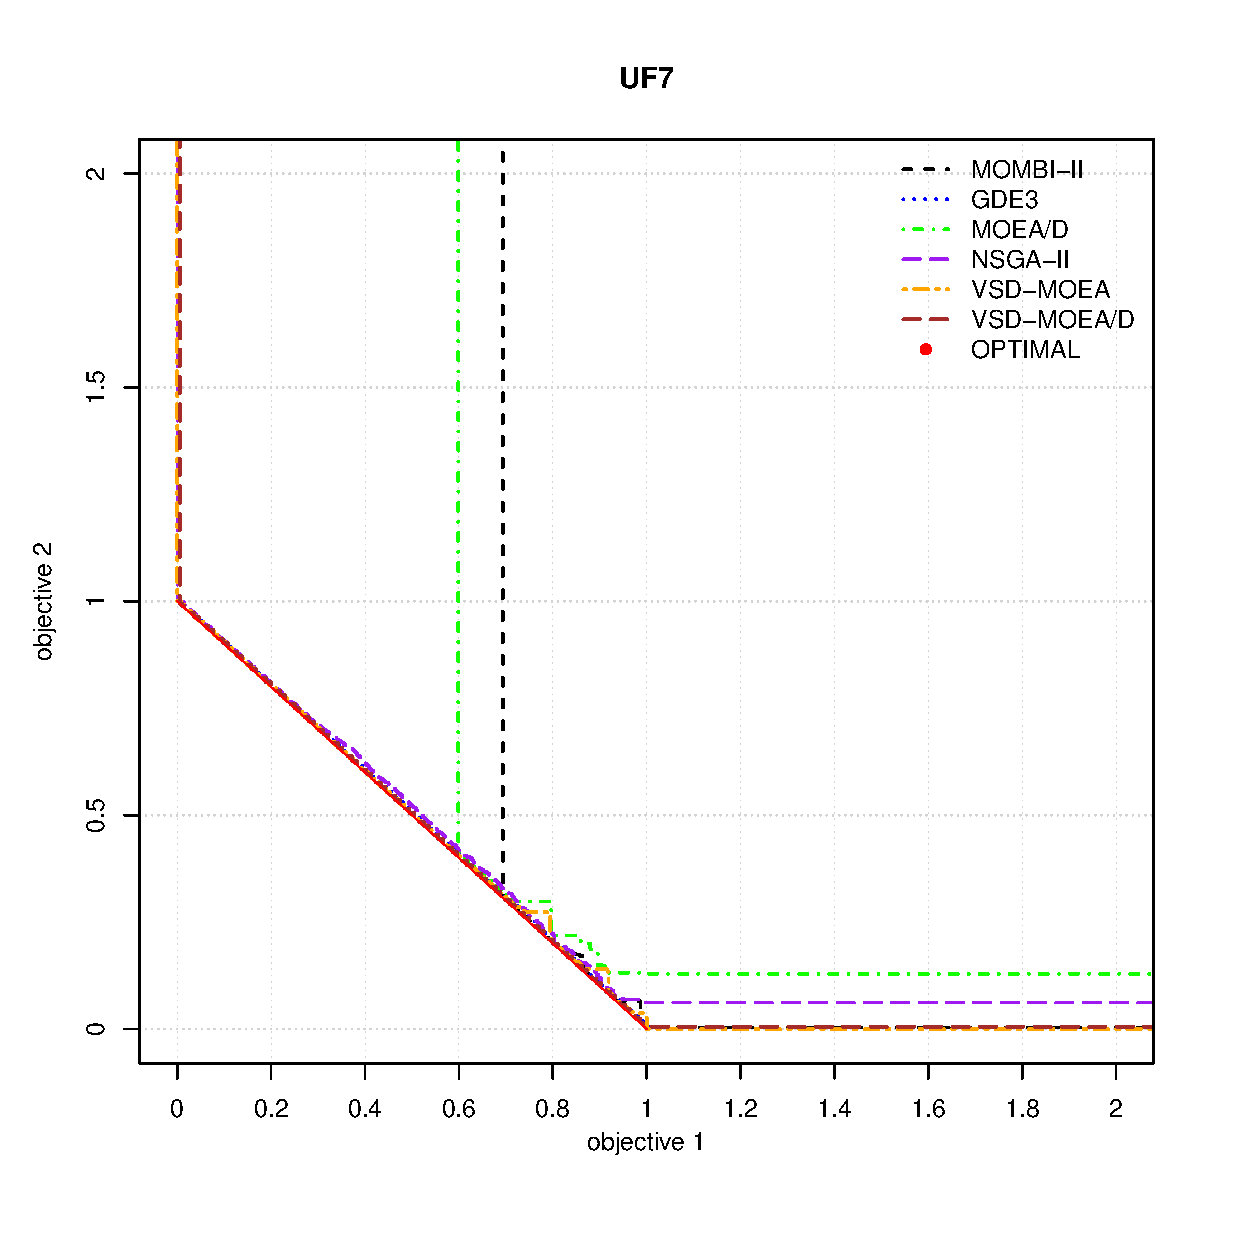
\includegraphics[scale=0.5]{Figures_Chapter2/UF7.eps} & \includegraphics[scale=0.5]{Figures_Chapter2/UF8.eps} \\
UF9 & UF10 \\
\includegraphics[scale=0.5]{Figures_Chapter2/UF9.eps} & \includegraphics[scale=0.5]{Figures_Chapter2/UF10.eps}
\end{tabular}%
}
\end{table}


% Please add the following required packages to your document preamble:
% \usepackage{graphicx}
\begin{table}[]
\centering
\caption{Problemas de prueba UF (CEC 2009)}
\label{tab:UF}
\resizebox{\textwidth}{!}{%
\begin{tabular}{|l|l|c|}
\hline
\multicolumn{1}{|c|}{Nombre} & \multicolumn{1}{c|}{Problema} & Dominio \\ \hline
UF1 & \begin{tabular}[c]{@{}l@{}}$ \begin{array}{lll} f_1&= x_1 + \frac{2}{|J_1|} \sum_{j \in J_1} [x_j - sin(6 \pi x_1 + \frac{j \pi}{n})]^2 \\  f_2 &= 1 - \sqrt{x_1} + \frac{1}{|J_2|} \sum_{j \in J_2} [x_j - sin( 6 \pi x_1 + \frac{j \pi}{n})]^2  \end{array}$\\ $J_1 = \{ j|j$ es impar y $2 \leq j \leq n \}$\\  $J_2 = \{ j|j$ es par con $2 \leq j \leq n \}$\end{tabular} & $[0, 1] \times [-1,1]^{n-1}$ \\ \hline
UF2 & \begin{tabular}[c]{@{}l@{}}$ \begin{array}{lll}f_1 &= x_1 + \frac{2}{|J_1|} \sum_{j \in J_1} y_j^2  \\ f_2 &= 1 - \sqrt{x_1} + \frac{1}{|J_2|} \sum_{j \in J_2} y_j^2,\end{array}$\\ $J_1$ y $J_2$ son los mismos que en UF1\\ $\begin{array}{lll}y_j =\begin{cases} x_j - [0.3x_1^2 cos(24 \pi x_1 + \frac{4 j \pi}{n}) + 0.6 x_1] cos( 6 \pi x_1 + \frac{j \pi}{n}) \quad j \in J_1 \\x_j - [0.3x_1^2 cos(24 \pi x_1 + \frac{4 j \pi}{n}) + 0.6 x_1] cos( 6 \pi x_1 + \frac{j \pi}{n}) \quad j \in J_2,\end{cases} \end{array}$\end{tabular} & $[0, 1] \times [-1,1]^{n-1}$ \\ \hline
UF3 & \begin{tabular}[c]{@{}l@{}}$\begin{array}{lll} f_1 &= x_1 + \frac{2}{|J_1|} ( 4 \sum_{j \in J_1} y_j^2 - 2 \prod_{j \in J_1} cos (\frac{20 y_j \pi}{ \sqrt[]{j}} ) + 2 ) \\  \\ f_2 &= 1 - \sqrt[]{x_1} + \frac{2}{|J_2|} ( 4 \sum_{j \in J_2} y_j^2 - 2 \prod_{j \in J_2} cos (\frac{20 y_j \pi}{ \sqrt[]{j}} ) + 2 ) \\ y_j &= x_j -  x_1^{ 0.5(1.0 + \frac{3(j-2)}{n-2}) }, \quad j=2, ..., n,\end{array}$\end{tabular} & $[0, 1]^n$ \\ \hline
UF4 & \begin{tabular}[c]{@{}l@{}}$\begin{array}{lll}\\ f_1&= x_1 + \frac{2}{|J_1|} \sum_{j \in J_1} h(y_j)\\ f_2&= 1 - x_1^2 + \frac{2}{|J_2|} \sum_{j \in J_2} h(y_j),\end{array}$\\ $J_1$ y $J_2$ son los mismos que en UF1\\ $\begin{array}{lll} y_j = x_j - sin( 6 \pi x_1 + \frac{j \pi}{ n} ), j=2, ..., n. \\ h(t) = \frac{|t|}{ 1 ++ e^{2 |t| }} \end{array}$\end{tabular} & $[0, 1] \times [-2,2]^{n-1}$ \\ \hline
UF5 & \begin{tabular}[c]{@{}l@{}}$\begin{array}{lll} f_1 &= x_1 +(\frac{1}{2N} + \epsilon) | sin(2 N \pi x_1) + \frac{2}{|J_1|} \sum_{j \in J_1} h(y_j)\\   f_2 &= 1 - x_1 + (\frac{1}{2N} + \epsilon) | sin(2 N \pi x_1) + \frac{2}{|J_2|} \sum_{j \in J_2} h(y_j) \end{array}$\\ $J_1$ y $J_2$ son los mismos que en UF1\\ $\begin{array}{lll} y_j = x_j - sin( 6 \pi x_1 + \frac{j \pi}{ n} ), j=2, ..., n.\\ h(t) = 2t^2 - cos(4 \pi t) + 1 \end{array}$\end{tabular} & $[0, 1] \times [-1,1]^{n-1}$ \\ \hline
UF6 & \begin{tabular}[c]{@{}l@{}}$\begin{array}{lll} f_1 &= x_1 + max \{ 0,2(\frac{1}{2N} + \epsilon ) sin(2N \pi x_1)\} +\\  &\frac{2}{|J_1|} ( 4 \sum_{j \in J_1} y_j^2 - 2 \prod_{j \in J_1} cos( \frac{20 y_j \pi}{\sqrt[]{j}} ) + 2)\\  f_2 &= 1 - x_1 + max \{ 0,2(\frac{1}{2N} + \epsilon ) sin(2N \pi x_1),\} +\\ & \frac{2}{|J_2|} ( 4 \sum_{j \in J_2} y_j^2 - 2 \prod_{j \in J_2} cos( \frac{20 y_j \pi}{\sqrt[]{j}} ) + 2)\end{array}$\\ $J_1$ y $J_2$ son los mismos que en UF1\\ $y_j= x_j - sin(6 \pi x_1 + \frac{j \pi}{n}), j=2,...,n.$\end{tabular} & $[0, 1] \times [-1,1]^{n-1}$ \\ \hline
UF7 & \begin{tabular}[c]{@{}l@{}}$\begin{array}{lll}\\ f_1 &= \sqrt[5]{x_1} + \frac{2}{|J_1|} \sum_{j \in J_1} y_j^2 \\ f_2 &= 1 - \sqrt[5]{x_1} + \frac{2}{|J_2|} \sum_{j \in J_2} y_j^2,\end{array}$\\ $J_1$ y $J_2$ son los mismos que en UF1\\ $y_j = x_j - sin(6 \pi x_1 + \frac{j \pi}{n} ), j=2,..., n$\end{tabular} & $[0, 1] \times [-1,1]^{n-1}$ \\ \hline
UF8 & \begin{tabular}[c]{@{}l@{}}$\begin{array}{lll}f_1 &= cos(0.5 x_1 \pi) cos(0.5 x_2 \pi ) + \frac{2}{|J_1|} \sum_{j \in J_1} (x_j - 2 x_2 sin(2\pi x_1 + \frac{j \pi}{n}))^2 \\ f_2 &= cos(0.5 x_1 \pi) sin(0.5 x_2 \pi ) + \frac{2}{|J_2|} \sum_{j \in J_1} (x_j - 2 x_2 sin(2\pi x_1 + \frac{j \pi}{n}))^2  \\ f_3 &= sin(0.5 x_1 \pi ) + \frac{2}{|J_3|} \sum_{j \in J_1} (x_j - 2 x_2 sin(2\pi x_1 + \frac{j \pi}{n}))^2 \end{array}$\\ $J_1 = \{ j|3 \leq j \leq n \}$, y $j-1$ es una multiplicación de 3, \\ $J_2 = \{ j|3 \leq j \leq n \}$, y $j-2$ es una multiplicación de 3\\ $J_3 = \{ j|3 \leq j \leq n \}$, y $j$ es una multiplicación de 3.\end{tabular} & $[0,1]^2 \times [-2, 2]^{n-2}$ \\ \hline
UF9 & \begin{tabular}[c]{@{}l@{}}$\begin{array}{lll}\\ f_1 &= 0.5[ max\{ 0,(1 + \epsilon) (1 - 4(2 x_1 - 1)^2 ) \} + 2 x_1] x_2 + \\ &\frac{2}{|J_1|} \sum_{j \in J_1} ( x_j - 2 x_2 sin(2 \pi x_1 + \frac{j \pi}{n}) )^2\\ f_2 &= 0.5[ max\{ 0,(1 + \epsilon) (1 - 4(2 x_1 - 1)^2 ) \} - 2 x_1 + 2] x_2 + \\ &\frac{2}{|J_2|} \sum_{j \in J_2} ( x_j - 2 x_2 sin(2 \pi x_1 + \frac{j \pi}{n}) )^2\\ f_3 &= 1 - x_2 + \frac{2}{|J_3|} \sum_{j \in J_3} ( x_j - 2 x_2 sin(2 \pi x_1 + \frac{j \pi}{n}) )^2,\end{array}$\\ $J_1$, $J_2$ y $J_3$ son los mismos que en UF9\\ $\epsilon = 0.1$\end{tabular} & $[0,1]^2 \times [-2, 2]^{n-2}$ \\ \hline
UF10 & \begin{tabular}[c]{@{}l@{}}$\begin{array}{lll}f_1 &= cos(0.5 x_1 \pi ) cos(0.5 x_2 \pi) + \frac{2}{|J_1|} \sum_{j \in J_1} [ 4 y_j^2 - cos( 8 \pi y_j) + 1] \\ f_2 &= cos(0.5 x_1 \pi ) sin(0.5 x_2 \pi) + \frac{2}{|J_2|} \sum_{j \in J_2} [ 4 y_j^2 - cos( 8 \pi y_j) + 1] \\ f_3 &= sin(0.5 x_1 \pi) + \frac{2}{|J_3|} \sum_{j \in J_3} [ 4 y_j^2 - cos( 8 \pi y_j) + 1]\end{array}$\\ $J_1$, $J_2$ y $J_3$ son los mismos que en UF9\\ $y_j = x_j - 2 x_2 sin( 2 \pi x_1 + \frac{j \pi}{n}), \quad j=3, ..., n$\end{tabular} & \multicolumn{1}{l|}{$[0,1]^2 \times [-2, 2]^{n-2}$} \\ \hline
\end{tabular}%
}
\end{table}


%% Please add the following required packages to your document preamble:
%% \usepackage{graphicx}
%\begin{table}[]
%\centering
%\caption{My caption}
%\label{my-label}
%\resizebox{\textwidth}{!}{%
%\begin{tabular}{|c|l|c|}
%\hline
%Nombre & \multicolumn{1}{c|}{Problema} & Dominio de los parámetros \\ \hline
%ZDT1 & $ \begin{array}{lll} f_1(x_1) &= x_1 \\g(x_2, ..., x_n) &= 1+9,\sum_{i=2}^n x_i / (n-1) \\h(f_1, g) &= 1 - \sqrt{f_1/g} \end{array}$ & $[0,1]$ \\ \hline
%ZDT2 & Igual que ZDT1, a excepción de $h = 1-(f_1 / g)^2$ & $[0,1]$ \\ \hline
%ZDT3 & Igual que ZDT1, a excepción de $h(f_1, g) = 1 - \sqrt{f_1/g} - (f_1 / g) sin( 10 \pi f_1)$ & $[0,1]$ \\ \hline
%ZDT4 & Igual que ZDT1, a excepción de $h(f_1, g) = 1 - \sqrt{f_1/g}$ & $ \begin{array}{lll}  x_1 \in [0,1] \\ x_2, ..., x_n \in [-5, 5] \end{array}$ \\ \hline
%ZDT6 & $ \begin{array}{lll} f_1(x_1) &= 1 - exp(-4 x_1) sin^6 (6 \pi x_1) \\g(x_2, ..., x_n) &= 1 + 9 \sum_{i=2}^n (x_i / (n-1))^{0.25} \\h(f_1, g) &= 1 - (f_1/g)^2 \end{array}$ & $[0,1]$ \\ \hline
%DTLZ1 & $ \begin{array}{lll}  f_1 &= (1+g) 0.5 \prod_{i=1}^{M-1} x_i \\ f_{m=2:M-1} &= (1+g) 0.5 (\prod_{i=1}^{M-m} x_i)(1 - y_{M-m+1}) \\ f_M &= (1+g) 0.5 (1-x_1) \\ g &= 100[x_M+\sum_{x_i \in x_M} (  (x_i - 0.5)^2 - cos(20 \pi (x_i - 0.5)) )] \end{array}$ & $[0,1]$ \\ \hline
%DTLZ2 & $ \begin{array}{lll}   f_1 &= (1+g) \prod_{i=1}^{M-1} cos(x_i \pi/2) \\   f_{m=2:M-1} &= (1+g) \left (  \prod_{i=1}^{M-m} cos(x_i \pi / 2)   \right ) sin(x_{M-m+1} \pi / 2)   \\   f_M &= (1+g) sin(x_1 \pi /2) \\   g &= \sum_{x_i \in x_M} (x_i -0.5)^2 \end{array}$ & $[0,1]$ \\ \hline
%DTLZ3 & Igual que DTLZ2, excepto que se utiliza la ecuación $g$ del DTLZ1 & $[0,1]$ \\ \hline
%DTLZ4 & Igual que DTLZ2, excepto que $x_i \in x$ es reemplazado por $x_i ^ \alpha$, donde $\alpha > 0$ & $[0,1]$ \\ \hline
%DTLZ5 & Igual que DTLZ2, excepto que $x_2, ..., x_{M-1} \in x $ son reemplazados por $\frac{1+2 g x_i}{2(1+g)}$ & $[0,1]$ \\ \hline
%DTLZ6 & Igual que DTLZ5, excepto que la ecuación para $g$ es reemplazada por $g = \sum_{x_i \in x_M} x_i^{0.1}$ & $[0,1]$ \\ \hline
%DTLZ7 & $ \begin{array}{lll} f_{m=1:M-1} &= x_m \\ f_M &= (1+g) \left (  M - \sum_{i=1}^{M-1} \left [ \frac{f_i}{1+g}(1 + sin(3 \pi f_i)) \right ] \right) \\ g &= 1+9 \sum_{x_i \in x_M} x_i /k \end{array}$ & $[0,1]$ \\ \hline
%\multicolumn{1}{|l|}{WFG1} & \begin{tabular}[c]{@{}l@{}}$\begin{array}{lll}      t^1_{i=1:k} &= x_i \\ t^1_{k+1:n} &= s\_linear(x_i, 0,35) \\ t^2_{i=1:k} &= x_i \\ t^2_{i=k+1:n} &= b\_flat(x_i, 0.8, 0.75, 0.85) \\ t^3_{i=1:n} &= b\_poly(x_i, 0.02) \\ t^4_{i=1:M-1} &= r\_sum(  \{ x_{(i-1)k/(M-1)+1},...,y_{ik/(M-1)} \}, \\  &\{ 2((i-1)k/(M-1)+1), ..., 2ik/(M-1) \} ) \\ t^4_M &= r\_sum( \{x_{k+1},...,y_n\}, \{ 2(k+1), ..., 2n \}) \\ h_{m=1:M-1} &= convex_m\\ \end{array}$\end{tabular} & $[0, 2 i]$ \\ \hline
%\multicolumn{1}{|l|}{WFG2} & \begin{tabular}[c]{@{}l@{}}Implementar $t^1$ del WFG1\\ $ \begin{array}{lll} t^2_{i=1:k}  &= x_i\\    t^2_{i =k+1:k+l/2} &= r\_nonsep(\{ x_{k+2(i-k)-1}, z_{k+2(i-k)}  \}, 2 )\\    t^3_{i=1:M-1} &= r\_sum( \{  x_{(i-1)k / (M-1) +1}, ..., x_{ik / (M-1)}  \}, \{1,...,1\} )\\    t^3_M &= r\_sum( \{ y_{k+1},..., y_{k+l/2}  \},\{1,...,1\} )\\    h_{m=1:M-1} &= convex_m\\    h_M &= disc_M ( \alpha = \beta =1, A = 5)\\  \end{array}$\end{tabular} & $[0, 2 i]$ \\ \hline
%\multicolumn{1}{|l|}{WFG3} & \begin{tabular}[c]{@{}l@{}}Implementar $t^1$, $t^2$ y $t^3$ del WFG2\\ $h_{m=1:M} = linear_m$\end{tabular} & $[0, 2 i]$ \\ \hline
%\multicolumn{1}{|l|}{WFG4} & \begin{tabular}[c]{@{}l@{}}$\begin{array}{lll}  t^1_{i=1:n} &= s\_multi(x_i, 30, 10, 0.35)\\   t^2_{i=1:M-1} &= r\_sum(\{ x_{(i-1)k / (M-1)+1},..., x_{ik / (M-1)}  \}, \{1,...,1\})\\   t^2_M &= r\_sum( \{ x_{k+1}, ..., x_n  \}, \{1,...,1\})\\   h_{m=1:M} &= concave_m\\ \end{array}$\end{tabular} & $[0, 2 i]$ \\ \hline
%\multicolumn{1}{|l|}{WFG5} & \begin{tabular}[c]{@{}l@{}}$t^1_{i=1:n} = s\_decept(x_i, 0.35, 0.001, 0.05)$\\ Implementar $t^2$ del WFG4 \\ $h_{m=1:M} &= concave_m$\end{tabular} & $[0, 2 i]$ \\ \hline
%\multicolumn{1}{|l|}{WFG6} & \begin{tabular}[c]{@{}l@{}}Implementar $t^1$ del WFG1\\ $\begin{array}{lll} t^2_{i=1:M-1} &= r\_nonsep(\{y_{(i-1)k / (M-1) +1}, ..., y_{ik / (M-1)}\}, k/(M-1))\\  t^2_M &= r\_nonsep(\{ y_{k+1}, ..., y_n \}, l)\\ h_{m=1:M} &=concave_m\\  \end{array}$\end{tabular} & $[0, 2 i]$ \\ \hline
%\multicolumn{1}{|l|}{WFG7} & \begin{tabular}[c]{@{}l@{}}$\begin{array}{lll} t^1_{i=1:k} &= b\_param(x_i, r\_sum(\{ x_{i+1}, ..., x_n \},\{1,...,1\}), \frac{0.98}{49.88}, 0.02, 50)\\    t^1_{i=k+1:n} &=x_i\\    \end{array}$\\ Implementar $t^1$ del WFG1\\ Implementar $t^2$ del WFG4\\ $h_{m=1:M} = concave_m$\end{tabular} & $[0, 2 i]$ \\ \hline
%\multicolumn{1}{|l|}{WFG8} & \begin{tabular}[c]{@{}l@{}}$\begin{array}{lll}   t^1_{i=1:k} &= x_i\\    t^1_{k+1:n} &= b\_param( x_i, r\_sum( \{ x_1,, ...., x_{i-1} \}, \{ 1,..., 1\} ) , \frac{0.98}{49.98}, 0.02, 50)\\   \end{array}$\\ Implementar $t^2$ del WFG1\\ Implementar $t^2$ del WFG4\\ $h_{m=1:M} = concave_m$\end{tabular} & $[0, 2 i]$ \\ \hline
%\multicolumn{1}{|l|}{WFG9} & \begin{tabular}[c]{@{}l@{}}$\begin{array}{lll}t^1_{i=1:n-1} &= b\_param( x_i, r\_sum(  \{ y_{i+1}, ..., y_n \}, \{1,...,1\} ), \frac{0.98}{49.98}, 0.02, 50 )\\ t^1_{n} &= x_n\\ t^2_{i=1:k} &= s\_decept(x_i, 0.35, 0.001, 0.05)\\ t^2_{i=k+1:n} &= s\_multi(x_i, 30, 95, 0.35)\\ \end{array}$\\ Implementar $t^2$ del WFG6\\ $h_{m=1:M} = concave_m$\end{tabular} & $[0, 2 i]$ \\ \hline
%\end{tabular}%
%}
%\end{table}
%


% Please add the following required packages to your document preamble:
% \usepackage{graphicx}
\begin{table}[H]
\centering
\caption{Propiedades de los problemas de prueba ZDT, DTLZ, WFG y UF}
\label{tab:Propiedades}
\resizebox{\textwidth}{!}{%
\begin{tabular}{|c|c|c|c|c|c|}
\hline
\textbf{Nombre} & \textbf{Separable} & \textbf{Modalidad} & \multicolumn{1}{l|}{\textbf{Geometría del frente de Pareto}} & \multicolumn{1}{l|}{\textbf{Distribución de las soluciones}} & \textbf{Número de objetivos} \\ \hline
ZDT1 & Si & Unimodal & Convexo & Uniforme & 2 \\ \hline
ZDT2 & Si & Unimodal & Concavo & Uniforme & 2 \\ \hline
ZDT3 & Si & Unimodal-Multimodal & Desconectado & Uniforme & 2 \\ \hline
ZDT4 & Si & Unimodal-Multimodal & Convexo & Uniforme & 2 \\ \hline
ZDT6 & Si & Multimodal & Concavo & Polinomial & 2 \\ \hline
DTLZ1 & Si & Multimodal & Lineal & Uniforme & N \\ \hline
DTLZ2 & Si & Unimodal & Concavo & Uniforme & N \\ \hline
DTLZ3 & Si & Multimodal & Concavo & Uniforme & N \\ \hline
DTLZ4 & Si & Unimodal & Concavo & Polinomial & N \\ \hline
DTLZ5 & - & Unimodal & Degenerado - Arco & Uniforme & N \\ \hline
DTLZ6 & - & Unimodal & Degenerado - Arco & Depende del parámetro & N \\ \hline
DTLZ7 & Si & Unimodal-Multimodal & Desconectado - Mixto & Uniforme & N \\ \hline
WFG1 & Si & Unimodal & Convexo - Mixto & Polinomial - Regiones planas & N \\ \hline
WFG2 & No & Unimodal-Multimodal & Convexo - Desconectado & Uniforme & N \\ \hline
WFG3 & No & Unimodal & Lineal - Degenerado & Uniforme & N \\ \hline
WFG4 & Si & Multimodal & Concavo & Uniforme & N \\ \hline
WFG5 & Si & Deceptivo & Concavo & Uniforme & N \\ \hline
WFG6 & No & Unimodal & Concavo & Uniforme & N \\ \hline
WFG7 & Si & Unimodal & Concavo & Depende del parámetro & N \\ \hline
WFG8 & No & Unimodal & Concavo & Depende del parámetro & N \\ \hline
WFG9 & No & Unimodal-Deceptivo & Concavo & Depende del parámetro & N \\ \hline
UF1 & - & - & Concavo & - & 2 \\ \hline
UF2 & - & - & Concavo & - & 2 \\ \hline
UF3 & - & - & Concavo & - & 2 \\ \hline
UF4 & - & - & Convexo & - & 2 \\ \hline
UF5 & - & - & Frente de 21 puntos & - & 2 \\ \hline
UF6 & - & - & Lineal & - & 2 \\ \hline
UF7 & - & - & Lineal & - & 2 \\ \hline
UF8 & - & - & Parabólico & - & 3 \\ \hline
UF9 & - & - & Planar & - & 3 \\ \hline
UF10 & - & - & Parabólico & - & 3 \\ \hline
\end{tabular}%
}
\end{table}

\subsection{Generar las soluciones óptimas}
Generar las soluciones óptimas de Pareto que corresponden a los problemas de prueba es un aspecto importante, ya que varias métricas utilizan estas soluciones óptimas como conjuntos de referencia.
%
Aunque se proporcionan las fórmulas para obtener los óptimos de pareto en los problemas multi-objetivo, se debe tener cuidado, principalmente porque una distribución de soluciones en el espacio de las variables no determina una distribución igual en el espacio objetivo, tal es el caso de los problemas WFG, que aunque proporcionan un generador de soluciones, las soluciones no tienen una distribución adecuada, principalmente en configuraciones que aumentan la complejidad.
%
Además la cantidad de puntos de referencia es afectado en caso de que el número de objetivos o el número de variables es elevado, ya que al generar puntos en base a una distribución uniforme podría no ser suficiente para representar adecuadamante al frente de Pareto.
%
Para resolver estos inconvenientes se implementa un método Quasi aleatorio, específicamente el método de Hammersley el cual produce una secuencia de números con baja discrepancia \citep{Joel:Hammersley, Joel:AlgoritmoHungaro}.
%
A diferencia de un generador de números aleatorios, implementar una secuencia de baja discrepancia genera puntos en el espacio de un modo más sistemático.
%
Ya que un clásico generador aleatorio, una misma área puede explorarse varias veces y otras no ser exploradas nunca, particularmente esta dificultad se incrementa considerablemente al aumentar la dimensión de los espacios.
%
El procedimiento que sugerido consiste en generar una secuencia de números en el espacio de soluciones óptimas por medio del método de Hammersley, posteriormente se implementa un proceso de filtrado, el cual consite en elimintar a los puntos más cercanos dada una tolerancia. 
%
Como se puede observar en la figura \ref{fig:Random} la cual es resultado de generar diez mil puntos en un espacio de tres dimensiones, en la parte izquierda de la fiigura los puntos se generan por medio de una distribución uniforme y en la parte derecha se generan por medio del método de hammersley, se puede observar que generar datos con una distribución uniforme puede provocar regiones aisladas.

\begin{figure}[H]
\centering
\scriptsize
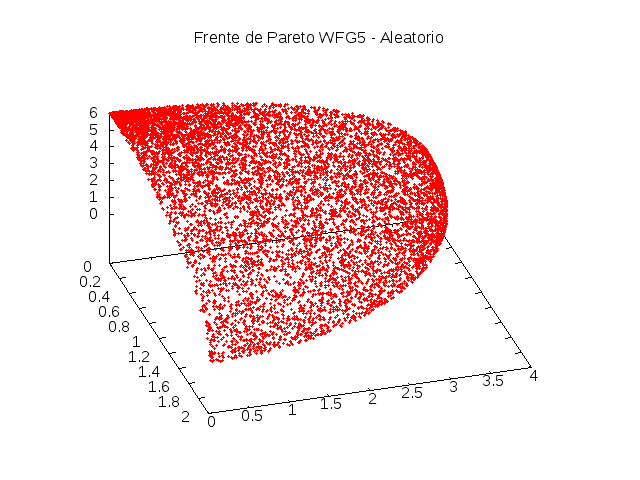
\includegraphics[scale=0.35]
{Figures_Chapter2/Random.png}
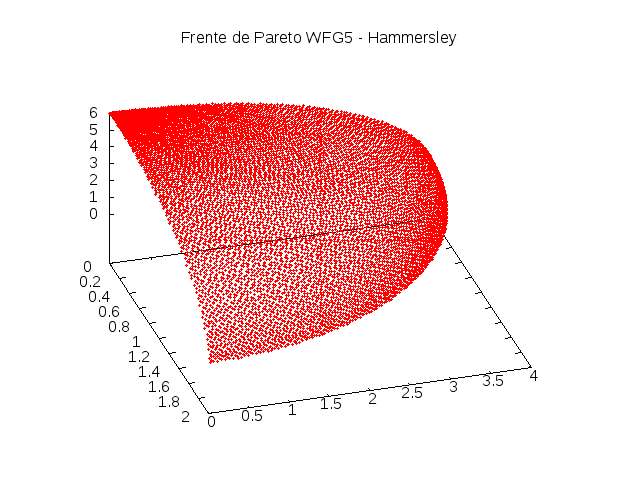
\includegraphics[scale=0.35]
{Figures_Chapter2/Hammersley.png}
\caption{Frente de Pareto problema WFG5, en la izquierda con un método aleatorio y con el método de Hammersley considerando diez mil puntos.}
\label{fig:Random}
\end{figure}


\section{Métricas}
En optimización multi-objetivo, se han desarrollado técnicas para medir el desempeño de las soluciones obtenidas.
%
Se han propuesto varios indicadores para evaluar la calidad del conjunto de soluciones no dominados \citep{Joel:EjemploFallaGD}.\\
%
En general los indicadores son métricas las cuales determinan el grado de convergencia al frente de Pareto y/o la diversidad de las soluciones en el frente de Pareto.
%
El indicador que se utiliza más frecuentemente es el hipervolumen \citep{Joel:ComparativeCaseStudy} . 
%
Esto se debe a que ningún otro indicador es \textit{Pareto compliant} \citep{Joel:HypervolumeRevisited}. 
%
Una característica importante que un indicador debería tener es ser \textit{Pareto compliant} \citep{Joel:ComparacionMetricas}, esto quiere decir que el indicador no debería contradecir el orden inducido por la relación de dominancia.
%
Así, dados dos conjuntos de soluciones $A$ y $B$ si $A \succeq B \land B \nsucc A$, entonces el valor del indicador de $A$ no debe ser peor que el valor del indicador $B$.
%
Para considerarse estrictamente \textit{compliant} se requiere que $A \succeq B \land B  \nsucc A$ implicando que el valor del indicador de $A$ es estrictamente mejor que el valor del indicador $B$, esto es:
\begin{equation*}
   A \succeq B \land B \nsucceq A \Rightarrow  I(A) > I(B)
\end{equation*}
%

%
En la literatura se ha descrito repetidas veces \citep{Joel:HypervolumeRevisited, Joel:EjemploFallaGD}  que con indicadores de tipo Pareto \textit{non-compliant} se pueden obtener resultados engañosos al momento de evaluar al conjunto de soluciones no dominadas. 
%
En el \citeyear{Joel:EjemploFallaGD} \citeauthor{Joel:EjemploFallaGD} demuestran que se pueden obtener resultados engañosos implementando la distancia generacional (GD).
%
En este contexto un conjunto de soluciones óptimas de Pareto se denotan por $P^*$ y el conjunto de aproximaciones por $Q$ compuestos por $M$ y $N$ puntos respectivamente.

\subsection{Distancia Generacional y Distancia Generacional Invertida}

La Distancia Generacional (GD - \cite{Joel:GD}) y la Distancia Generacional Invertida  son indicadores considerados Pareto \textit{non-compliant}, y para ser implementados es requerido el conjunto óptimo de Pareto.
%
El GD está diseñado para obtener la distancia promedio de cada solución al punto de referencia más cercano. 


Por otra parte la Distancia Generacional Invertida (IGD) fue propuesta por \cite{Joel:ParallelizationMOEA, Joel:SwarmOptimizerDiversity}. Sin embargo ya se habían propuesto indicadores similares por \citeauthor{Joel:SimulatedAnnealingMetaheuristic} en \citeyear{Joel:SimulatedAnnealingMetaheuristic}.\\
%
El IGD es la distancia promedio de cada punto de referencia a su solución más cercana.
%
Así, si se tiene un conjunto de puntos utilizados como referencia, los cuales estén bien distribuidos en el frente de Pareto, un valor pequeño del IGD sugiere una buena convergencia de las soluciones al frente de Pareto y una buena distribución en relación al frente de Pareto.
\begin{equation}
\begin{split}
GD (P^*, Q) = \frac{1}{|N|}\left(  \sum_{i=1}^{|N|} d_i^p  \right) ^{1/p} \qquad
IGD (P^*, Q) = \frac{1}{|M|}\left(  \sum_{i=1}^{|M|} \hat{d}_j^p  \right) ^{1/p}
\end{split}
\end{equation}
Donde $d_i$ denota la distancia Euclídea entre la solución $y_i \in Q$ y el punto de referencia más cercano del conjunto $P^*$ y $\hat{d_i}$ denota la distancia entre el punto de referencia $x_i^* \in P^*$ a la solución más cercana del conjunto $Q$. 
% 
Recientemente \citeauthor{Joel:HausdorffDistance} propusieron una modificación al GD y al IGD, donde argumentan que conforme aumenta el número de puntos $M$, la calidad en la aproximación "mejora", aunque la aproximación aparentemente no ha cambiado, tratándose de un falso positivo.
%
Esto es demostrado, asumiendo que el conjunto de distancias $d_i$ (para el caso del GD) sean 1 y dada una muestra de $N$ soluciones, entonces:
\begin{equation*}
  GD(P^*, Q) = \frac{1}{|N|}\left( \sum_{i=1}^{|N|} d_i^p  \right) ^{1/p} = \frac{ \Vert (1,...,1)^T \Vert_p }{N} = \frac{\sqrt[p]{N}}{N} 
\end{equation*}
%
Se puede observar que:
\begin{itemize}
\item Al incrementar el número $N$ de puntos, la calidad que pertenece a la aproximación \textit{mejora} aunque aparentemente no ha cambiado.
\item La secuencia de puntos convergen a una aproximación "perfecta", esto es:
\begin{equation*}
\begin{split}
  \lim_{N \to \infty} GD( P^*, Q) = 0 
\end{split}
\end{equation*}
\end{itemize}
Lo mismo ocurre para el IGD, al considerar más puntos de referencia.
%
Para evitar el efecto mencionado, se propone la modificación al indicador, conocido como la potencia media para promediar las distancias:
\begin{equation}
\begin{split}
& GD_P(P^*, Q) = \left( \frac{1}{|N|}  \sum_{i=1}^{|N|} d_i^p  \right) ^{1/p} = \frac{ \Vert d_i \Vert_p }{\sqrt[p]{N}}  \\
& IGD_P(P^*, Q) = \left( \frac{1}{|M|}  \sum_{i=1}^{|M|} \hat{d}_j^p  \right) ^{1/p} = \frac{ \Vert \hat{d}_j \Vert_p }{\sqrt[p]{N}}  
\end{split}
\end{equation}
%
Esta modificación evita que al aumentar el número de soluciones (en el caso de GD) o al momento de aumentar el número de puntos de referencia (en el caso del IGD) la calidad del indicador se vea afectado.
%

%
Sin embargo como ya se explicó anteriormente al ser estas métricas Pareto \textit{non-compliant}, existen escenarios en que la estimación puede ser cuestionable, por ejemplo en la figura \ref{fig:IGD_Fallo} donde el conjunto de soluciones A y B evaluados con el IGD son 3.71 y 2.59 respectivamente, se observa que aunque el conjunto de soluciones A tenga más puntos cercanos a los  puntos de referencia la estimación de la métrica es mejorado por el conjunto de soluciones B.

\begin{figure}[H]
\centering
\scriptsize
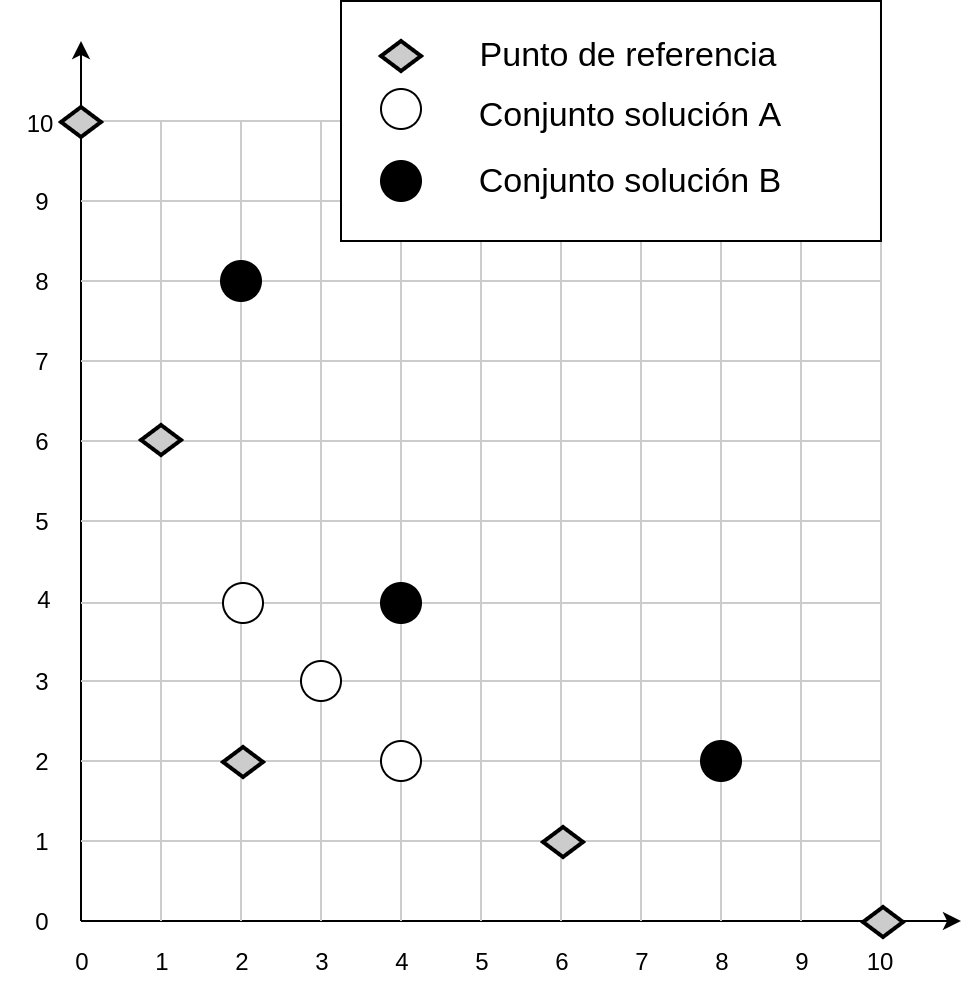
\includegraphics[scale=0.2]
{Figures_Chapter2/IGD_Problema.png}
\decoRule
\caption{Ejemplo con 5 puntos de referencia IGD.}
\label{fig:IGD_Fallo}
\end{figure}
%
En lugar del IGD se propone la distancia generacional invertida modificada (IGD+) propuesta por \citeauthor{Joel:IGDPlus_And_GDPlus} en el \citeyear{Joel:IGDPlus_And_GDPlus}, la cual es considerada como \textit{Weak Pareto compliance}, este indicador consiste en:


\textit{Si una solución es dominada por un punto de referencia, entonces se utiliza la distancia Euclídea sin alguna modificación. Sin embargo, si la solución y el punto de referencia son no dominados entre sí, entonces se calcula la mínima distancia desde el punto de referencia a la región dominada por la solución.}
%

La forma del IGD+ es similar al IGD propuesto previamente, a diferencia que la distancia Euclídea es modificada, de la siguiente manera:
\begin{itemize}
\item En problemas de minimización es \[d^+(z,a) = \sqrt{d_1^2 + ... + d_m^2} = \sqrt{max\{a_1 - z_1, 0\}^2+...+max\{a_m - z_m, 0\}^2}   \]
\item En problemas de maximización es \[d^+(z,a) = \sqrt{d_1^2 + ... + d_m^2} = \sqrt{max\{z_1 - a_1, 0\}^2+...+max\{z_m - a_m, 0\}^2}\]
\end{itemize}
%

\subsection{Distancia promedio de Hausdorff $\Delta_p$}
La distancia de Hausdorff $d_H$ es una herramienta utilizada para medir la distancia entre diferentes objetos \cite{Joel:HausdorffDistance}.
%
A excepción de trabajos teóricos, esta distancia no es muy utilizada en el ámbito multi-objetivo, la mayor razón es que probablemente $d_H$ penaliza los valores más atípicos de un conjunto de puntos, lo cual produce que una ``buena'' aproximación que contiene al menos un dato atípico sea considerada como una ``mala'' aproximación.
%
Un forma para remediar esto es promediando las distancias de los elementos que pertenecen a los conjuntos, guiando a una ``distancia promedio de Hausdorff''.
%
\begin{equation}
\Delta_p(P) = max \{ GD_p(P^*, Q), IGD_p(P^*, Q) \}
\end{equation}
%
Los autores \citeauthor{Joel:HausdorffDistance} argumentan que una propiedad importante que debe poseer una métrica es la de satisfacer la desigualdad del triángulo.
%
Sin embargo se debe tener cuidado que al promediar las distancias es posible violar dicha propiedad.
%
El efecto que tiene el parámetro $p$ sobre la métrica $\Delta_p$ es la clave para manejar los datos atípicos, ya que un valor pequeño de $p$ tiene un mayor efecto en el promedio y existe una menor influencia de los datos atípicos.
%
De otra forma, si $p$ es incrementado, los datos atípicos influyen más en la métrica $\Delta_p$.
%
En el caso extremo donde $p \rightarrow \infty$, sólo son consideradas las distancias que corresponden a los puntos más lejanos.
%
En un análisis práctico se concluye que las violaciones de la desigualdad del triángulo disminuyen conforme aumenta el parámetro de $p$, de igual forma sucede como conforme incrementa el número de elementos en los conjuntos considerados.
%
Esto demuestra una razón por los cual en la literatura no se observan análisis sobre la violación de la desigualdad del triángulo.
%
Ya que para usos prácticos se observa que $\Delta_p$ debería ser suficiente ''similar`` a una métrica.


\subsection{Distancia al vecino más cercano - DCN}
El DCN (\textit{Distance to the Closest Neighbor}) es una métrica que normalmente se utiliza en algoritmos evolutivos que mantienen algún mecanismo para gestionar la diversidad \citep{Joel:DCN, Joel:MultiDynamic}.\\
El valor de esta métrica indica el grado de diversidad que existe en una población, esto se realiza promediando las distancias a los individuos más cercanos de cada individuo.
Para obtener el valor de esta métrica en relación al individuo $i$, se considera al individuo $j$ con menor distancia de la población $Q$.

\begin{equation}
DCN(i) = arg_{min} d(i,j ) \forall j \in Q, i \neq j
\end{equation}

\subsection{Distancia media (ADI)}
La distancia media  \citep{Joel:DCN, Joel:MultiDynamic} de un determinado individuo $i$, consiste en promediar todas las distancias a los demás individuos en la población $Q$.
\begin{equation}
ADI(i) = \frac{1}{|Q|} \sum_{j \in Q,  i \neq j}  d_{i,j}
\end{equation}

A diferencia del DCN la distancia media (\textit{Average Distance Individuals}), proporciona una estimación del centro de masa de todas las distancias, por lo que es más robusto, como ejemplo se observa un caso donde existe un punto atípico o muy lejano a los demás y el resto se ubican muy cercanos entre sí, entonces con el DCN el efecto del punto atípico se considera sólo una vez, por otro lado en el ADI este dato atípico participa en la estimación de cada punto, ahora si el número de puntos cercanos aumenta considerablemente, se observa que en la métrica del DCN el efecto del punto atípico disminuye considerablemente, y en contraparte en el ADI no pierde fuerza la distancia del punto atípico. 
%
Esto se puede demostrar visualizando los $N$ puntos en una recta (Figura \ref{fig:Recta_DCN}), donde un punto atípico $C$ se ubica en un lugar muy lejano del resto, además los $N-1$ puntos están acotados por $[L_I, L_S]$ y están equi-espaciados entre sí con una distancia de $k = \frac{L_S - L_I}{ N-2 }$. Promediando la métrica DCN de toda la población $Q$ se tiene:
%
\begin{equation}
   \begin{split}
      DCN &= \frac{ (N-1)(k) + C - L_S }{N} = \frac{(N-1)(L_S-L_I)}{(N)(N-2)} + \frac{C- L_S}{N} \\
      			 &= \lim_{N \rightarrow \infty} \frac{(N-1)(L_S-L_I)}{(N)(N-2)} + \frac{C- L_S}{N} \\ 
      			 &= \lim_{N \rightarrow \infty} \frac{(N-1)(L_S-L_I)}{(N)(N-2)}
   \end{split}
\end{equation}
Esto demuestra que el punto $C$ pierde efecto en la métrica del DCN conforme incrementa el número de individuos.
%
En el caso del ADI, se tiene:
\begin{equation}
\begin{split}
	ADI &= \frac{1}{N} \sum_{j=1}^N \left [ (\mu_j + C - x_j ) \frac{1}{N-1} \right  ] \\
		    &= \frac{1}{N} \left [  \frac{  \sum_{j=1}^N   \mu_j}{ N-1}  +  \frac{  \sum_{j=1}^N   C - x_j }{ N-1}  \right  ]
\end{split}
\end{equation}
Donde $\mu_j$ es la suma de todas las distancias entre el punto $x_j$ y los demás $N-2$ puntos (excepto $C$), se puede observar que conforme aumenta el número de puntos en el área del cluster, la distancia hacia el punto $C$ aún tiene influencia.

\begin{figure}[H]
\centering
\scriptsize
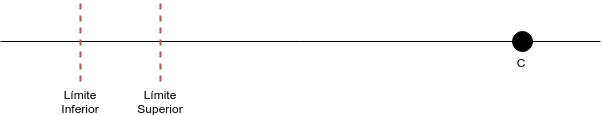
\includegraphics[scale=0.4]
{Figures_Chapter2/RECTA_DCN_ADI.png}
\decoRule
\caption{El punto obscuro representa al punto atípico $C$.}
\label{fig:Recta_DCN}
\end{figure}

\subsection{Hipervolumen HV}
Esta métrica calcula el volúmen (en el espacio objetivo) cubierto entre las soluciones obtenidas y un punto de referencia \citep{Joel:Lebesgue_Measure}. 
%	
El indicador del hipervolumen de un conjunto de soluciones aproximadas $Q$ y basado en un punto de referencia $r$ se define de la forma:
\begin{equation}
HV(Q, r) = \mathcal{L}(  \cup_{q \in Q} \{ q^,  | q \prec q^, \prec r  \}  )
\end{equation}
Donde  $\mathcal{L}$ es la medición de Lebesgue de un conjunto.

La contribucion del HV de una solucion $q \in Q$ individual refleja la influencia de un solo punto en la calidad del conjunto aproximado y es definido como:
\begin{equation}
C_{HV}(q,Q,r) = HV(Q,r) - HV(Q \backslash \{ q\}, r)
\end{equation}
El indicador del HV es el único indicador conocido como estrictamente Pareto \textit{compliant} con la relación de dominancia. 
\subsection{Indicador R2}
La familia de indicadores $R$ \citep{Joel:R2_Many_Objective}, estan basados en funciones de utilidad las cuales realizan un mapeo de un vector $\vec{y} \in \Re^m$ a un valor de utilidad escalar $u \in \Re$.
%
Normalmente en este indicador es preferido al HV, por dos razones: el tiempo de ejecución del HV es exponencial con respecto al número de objetivos \citep{Joel:ReferencePointBasedNonDominateSortingApproach} y las distribuciones obtenidas por el HV están sesgados hacia las regiones que forman un ángulo recto del frente de Pareto \citep{Joel:OnPropertiesR2Indicator}.
%
Por otro lado el indicador R2 genera soluciones con una distribución más uniforme.

\begin{Classic}
Para un conjunto finito y discreto $U$ y una distribución uniforme $p$ sobre $U$, el indicador $R2$ puede ser:
\end{Classic}
\begin{equation}
R2(R, Q, U) = \frac{1}{|U|} = \sum_{u \in U} \left ( max_{r \in R} \{ u(r) \} - max_{q \in Q}\{u(q)\} \right )
\end{equation}

Dado que el primer sumando es una constante, si se sume que $R$ es una constante por simplicidad se tiene:
\begin{equation}
R2(R, Q, U) = \frac{1}{|U|} = \sum_{u \in U} \left ( - max_{q \in Q}\{u(q)\} \right )
\end{equation}


Basado en la función de pesos estándar de Tchebycheff:
\begin{Classic}
El indicador $R2$ de una solución $Q$ para un conjunto de pesos y un punto utópico $Z^*$ se define:
\end{Classic}
\begin{equation}
R2(Q, \Lambda, z^*) = \frac{1}{|\Lambda|} \sum_{\lambda \in \Lambda} min_{q \in Q} \{ max \{ \lambda_j | z_j^* - q | \} \}
\end{equation}
donde $\Lambda$ está conformado por un conjunto de vectores de pesos $\vec{\lambda}$.\\
%
La contribución del una solución $q \in Q$ es definido de la forma:
\begin{equation}
C_{R2}(q, Q, \Lambda, z^*) = R2(Q, \Lambda, z^*) - R2(Q \backslash \{q\}, \Lambda, z^*)
\end{equation}
En el caso de Tchebycheff puede ser escrito de la forma:
\begin{equation}
\begin{split}
C_{R2}(q, Q, \Lambda, z^*) =  \frac{1}{|\Lambda|} \sum_{\lambda \in \Lambda} ( min_{b \in Q} \left \{ max_{j \in \{1,...,m\}} \{ \lambda_j | z_j^* - b_j\} \right \} -
	\\   min_{b \in Q \backslash\{q\} } \left \{ max_{j \in \{1,...,m\}} \{ \lambda_j | z_j^* - b_j\} \right \}  )  
\end{split}
\end{equation}

\subsection{Superficies de cubrimiento}

Ya que los MOEAs funcionan por medio de un proceso estocástico, para evaluar su desempeño de una forma más generalizada, se construye una muestra por medio del resultado final de varias ejecuciones \footnote{Cada ejecución se realiza con una semilla distinta para el generador de números pseudoaleatorios.} \citep{Joel:ComparisonStochasticSurfaces}.
%
Una vez obtenida la muestra, se puede hacer una estimación estadística sobre la calidad lograda en una fracción de la muestra.
%
Por ejemplo la calidad promedio de la muestra, es la mejor estimación que un algoritmo puede alcanzar en un 50\% de las ejecuciones y de forma similar para otros cuantiles.
%

En el ámbito multi-objetivo específicamente en problemas relacionados con dos objetivos se utiliza gráficamente lo que se conoce como \textit{resumen de las superficies de cubrimiento}, aunque para mayores dimensiones también se han propuesto técnicas basadas en grids y proyecciones para generar superficies de cubrimiento \citep{Joel:AttainmentSurface}.
%
Una superficie de cubrimiento es la región generada en base a los puntos no dominados obtenidos por una ejecución, esto se realiza dibujando un límite en el espacio objetivo el cual separa el espacio dominado por o equivalente a cada uno de los puntos obtenidos, como se muestra en el cuadro de la parte superior izquierda de la figura  \ref{fig:AttainmentSurfaces}, se observa que la superficie de cubrimiento está conformada por un conjunto de lineas rectas las cuales se unen con las soluciones de una ejecución.
%
Así, una superficie de cubrimiento combina información sobre la calidad y la distribución de los puntos no dominados.
%
Una ventaja de las superficies de cubrimiento en comparación a simplemente graficando los puntos, es en el caso en que se muestran múltiples ejecuciones.\\
%
En el caso de múltiples superficies de cubrimiento se genera un resumen el cual es definido como la unión de todas las superficies.
%
Por lo que un resumen de las superficies de cubrimiento, sintetiza un conjunto de aproximaciones, y una superficie de cubrimiento es sólo una superficie definida por sólo un conjunto aproximado como resultado a una ejecución.
%
Visualmente este proceso consiste en ubicar líneas diagonales que cortan todas las superficies de cubrimiento como se muestra en el cuadro de la parte superior derecha de la figura \ref{fig:AttainmentSurfaces}, donde la línea diagonal inferior intersecta las superficies de cubrimiento en cinco puntos distintos, y esos puntos están ordenados a lo largo de la diagonal, así contando de izquierda a derecha los puntos de intersección en la línea diagonal primero se encuentra la mejor superificie de cubrimiento y en la última intersección la peor superficie de cubrimiento. 
%
Haciendo que cada intersección $s$ de la diagonal  con cada superficie de cubrimiento conforme los mejores resultados logrados precisamente en $s$ veces del total de ejecuciones. 
%
Utilizando muchas líneas diagonales se podría realizar una aproximación de todas las metas logradas, siendo precisamente en $s$ veces del total de ejecuciones, como ejemplo en la figura \ref{fig:AttainmentSurfaces} en la parte inferior se muestran las superficies logradas con $s= \{1, 2, 3, 4, 5\}$ que corresponde a $20\%, 40\%, 60\%, 80\%, 100\% $ respectiamente.

\begin{figure}[H]
\centering
\scriptsize
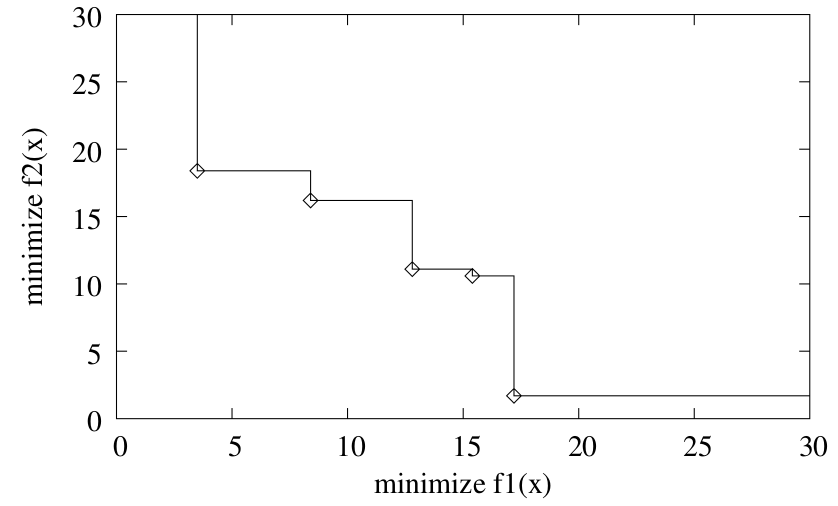
\includegraphics[scale=0.2]
{Figures_Chapter2/Surface.png}
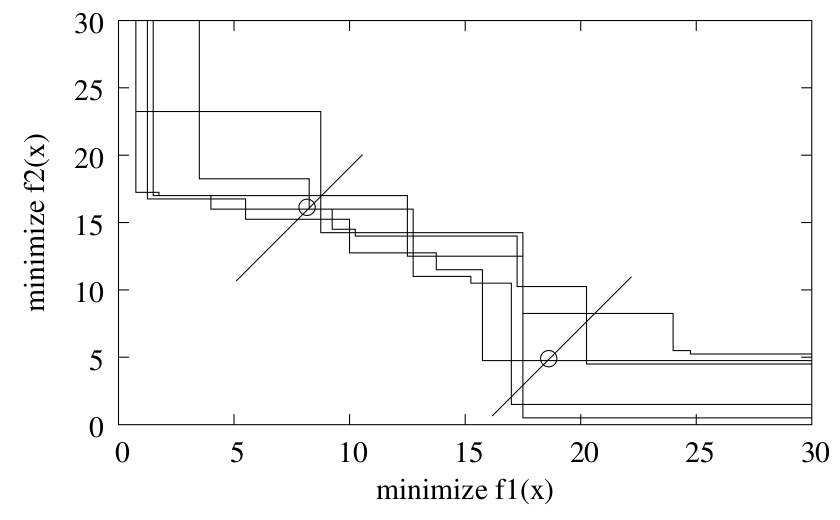
\includegraphics[scale=0.2]
{Figures_Chapter2/Surfaces.png}
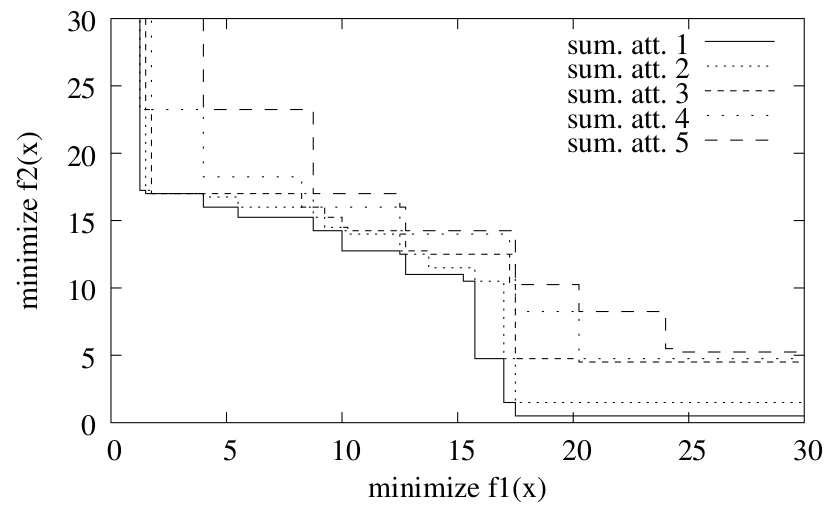
\includegraphics[scale=0.2]
{Figures_Chapter2/AttainmentSurfaces.png}
\decoRule
\caption{En la imágen superior izquierda se muestra una superficie de cubrimiento de una ejecución, en la imágen superior derecha se presentan las superficies de varias ejecuciones y en la imágen inferior se presenta el resumen de las superficies de cubrimiento logradas a $1, 2, 3, 4, 5$ que corresponde a $20\%, 40\%, 60\%, 80\%, 100\% $.}
\label{fig:AttainmentSurfaces}
\end{figure}

 
\chapter{Algoritmo de Diversidad basado en Dominancia} % Main chapter title

\label{Chapter3}

\section{Introducción}

Los algoritmos evolutivos (EA) son considerados como uno de los enfoques más prometedores en distintos problemas de optimización, tanto en dominios continuos como en discretos.
%
Además, se han vuelto bastante populares en las últimas décadas en parte por el incremento de las capacidades de cómputo.
%
Por lo tanto los EAs son utilizados ampliamente en diversas áreas de estudio y aplicaciones del mundo real.
%

%

Se ha demostrado que el rendimiento de un algoritmo evolutivo es afectado por falta de soluciones diversas.
%
Así, los algoritmos diagnosticados con problemas de diversidad pueden guiar el proceso de búsqueda a regiones complicadas, por lo tanto todos los miembros de la población son situados en una parte reducida del espacio de búsqueda, siendo distinta de la región de soluciones óptimas, además los componentes del algoritmo no permiten escapar de estas regiones, en el ámbito mono-objetivo esto es un inconveniente y es definido como convergencia prematura (\cite{Joel:Crepinsek}).
%
Además, se ha demostrado que un algoritmo evolutivo el cual proporciona un balance entre intensificación y exploración puede generar resultados de alta calidad e inclusive mejores que el promedio de algoritmos.
%
Por otra parte si la población es muy diversa, entonces la fase de explotación puede ser afectada, en consecuencia la convergencia del algortimo es muy lenta, proporcionando soluciones muy lejanas de la región óptima.
%
Por lo tanto \citeauthor{Joel:mahfoud1995niching} en \citetitle{Joel:mahfoud1995niching} define el concepto de diversidad útil como las cantidades de diversdad que proporcionan soluciones de calidad.
%Además el efecto que tiene la diversidad por parte de las soluciones en un algortimo evolutivo es evidente en la calidad de las soluciones, como es expliaco por ... en REF.
%

En la búsqueda de preservar un balance entre exploración e intensificación por parte del proceso evolutivo, se han desarrollado algoritmos mediante distintas estrategias, de esta forma se desea evitar el incoveniente de la convergencia prematura, los principales mecanismos utilizados son operadores de mutación disruptivos, tamaño de población variada, esquemas de reinicio, emparejamiento especial de padres (\cite{Joel:MOEAD_AMS}), modelos explícitos de seleccion (\cite{Joel:MULTI_DYNAMIC}), entre otros.
%
Sin embargo, no siempre se entiende plenamente la forma en que la exploración y la explotación se promueven en un EA, y dependen de una variante muy específica como parte de la estrategia implementada.
%
Por ejemplo, mientras en algunos esquemas el operador de mutación se encarga de promover la exploración (\cite{Joel:herrera2003fuzzy, Joel:CHC}), en otros casos esta tarea es asignada al operador de cruce (\cite{Joel:sivanandam2007introduction}). 


Aunque este trabajo se enfoca en la optimización multi-objetivo, las estrategias aquí presentadas pueden ser implementadas en el ámbito mono-objetivo sin cambios significativos.
%
%%%Se explican las secciones de este capítulo.

Inicialmente se mencionan algunas de las estrategias usadas para administrar la diversidad en el optmización mono-objetivo y multi-objetivo.
%
Posteriormente se explica el algoritmo propuesto en el ámbito multi-objetivo, considerado como el primer algoritmo basado en dominancia que administra la diversidad en las variables de decisión de forma explícita.
%
%
Adicionalmente se realiza una análisis de los beneficios y las desventajas del algoritmo propuesto, así mismo dando importancia a la diversidad en el espacio objetivo se presenta la fase de reemplazo que conforma parte del algoritmo VSD-MOEA y además se explica una simulación de los pasos involucrados en la fase de remplazo.
%
Por otra parte se propone la distancia de mejoría que está basada en el indicador IGD+, la cual es considerada como débilmente \textit{Pareto Compliance}.
%
Al final se muestra una simulación del VSD-MOEA junto al estado del arte en la problema de prueba WFG5 cuya principal característica es su transformación con propiedades deceptivas.

\section{Diversidad en el espacio de las variables en MOEAs}

En optimización estocástica, específicamente en el caso mono-objetivo, se ha desarrollado una variedad de algoritmos evolutivos con el propósito de tratar aspectos relacionados con la falta de diversidad, específicamente la convegencia prematura (\cite{Joel:Crepinsek}).
%
Algunos de los algoritmos populares que están relacionados con temas de diversidad son Saw-Tooth (\cite{Joel:SAWTOOTH}), CHC (\cite{Joel:CHC}) y Multi-Dynamic (\cite{Joel:MULTI_DYNAMIC}).
%
Este último relaciona el manejo de diversidad en el espacio de las variables con el criterio de paro establecido. % \cite{Joel:segura2016improving}.
%
De esta forma, y dependiendo del criterio de paro, en las fases iniciales se promueve un mayor nivel de exploración y conforme van transcurriendo las generaciones se realiza un cambio gradual para obtener un mayor nivel de intensificación.
%
Este control se puede realizar desde distintos enfoques, y se ha visto experimentalmente que actuar sobre varias fases puede ser beneficioso (\cite{Joel:ANovelDiversityBasedEAForTheTSP}).
%
Este tipo de métodos se han vuelto exitosos en optimización mono-objetivo, proporcionando el desarrollo de optimizadores que actualmente han encontrado los mejores resultados en varios problemas conocidos, como es el problema de ordenación lineal, el problema de asignación de frecuencias \citetitle{Joel:Dynamic_FAP}, el problema del Sudoku \citetitle{Joel:Dynamic_Sudoku}, el problema del agente viajero \citetitle{Joel:ANovelDiversityBasedEAForTheTSP}, entre otros.
%


En optimización multi-objetivo es posible encontrar los mismos inconvenientes que en problemas mono-objetivo, además al considerar varios objetivos que usualmente están en conflicto es necesario mantener soluciones diversas.
%
Así, un problema multi-objetivo está compuesto por dos espacios, el primero consiste en el espacio de las variables y sus respectivas imagenes conforman el espacio objetivo.
%
Además, no existe una correspondencia directa entre la diversidad de los dos espacios (\cite{shir2009enhancing}), esto quiere decir que un grado determinado de diversidad en el espacio objetivo no implica que siempre existirá un grado determinado de diversidad en el espacio de las variables.

% 
En todos los problemas multi-objetivo no existe una relación identica entre ambos espacios, debido a esto los MOEAs están diseñados principalmente para mantener diversidad en el espacio objetivo, perdiendo la influencia directa que existe por parte de la diversidad en espacio de las variables.

%
Actualmente ya existen varios trabajos que proporcionan relevancia a la diversidad en el espacio de las variables. % \citetitle{Joel:GECCO17}.
%
Una estrategia popular consiste en aplicar restricciones para realizar el emparejamiento de los individuos (\cite{Joel:MOEAD_AMS}), en base a varios estudios presentados en \citetitle{Joel:STUDY_MATTING_RESTRICTION} por \citeauthor{Joel:STUDY_MATTING_RESTRICTION}, donde se define una restricción de emparejamiento específicamente con soluciones cercanas o similiares en el espacio de las variables, debido a que emparejar dos individuos alejados tiende a generar individuos distantes y no útiles en el espacio de búsqueda.
%
Otra alternativa consiste en implementar esquemas de reinicios (\cite{ joel:jaeggi2008development, Joel:Improved_Multiobjective_Diversity_Control_Oriented_Genetic_Algorithm}).
%
Sin embargo en el caso multi-objetivo no se ha establecido una propuesta en donde la diversidad sea administrada de forma explícita y que dependa del criterio de paro.
%


En base al estudio de diversidad realizado por \citeauthor{Joel:GECCO17} en \citetitle{Joel:GECCO17} se ha comprobado que los MOEAs poseen problemas de diversidad.
%
Específicamente en este capítulo se utiliza el mismo principio que en \citeauthor{Joel:MULTI_DYNAMIC}, que está diseñado especialmente para problemas de un solo objetivo y administra la diversidad en el espacio de las variables de forma explícita. 

\section{Trabajos relacionados}

A través de las últimas décadas se han presentado varios trabajos de tipo multi-objetivo que están relacionados con promover soluciones diversas en el espacio de las variables, así los primeros trabajos surgieron con el propósito de resolver funciones objetivo de tipo multi-modal (\cite{preuss2006pareto}).
%In the MOEAs literature several analyzes of diversity in decision space are presented, in particular some of them are oriented to solve multi-modal objective functions \cite{preuss2006pareto}.
%
En especial, esta categoría de algoritmos pueden ser de interés en problemas de aplicación real, ya que es necesario proporcionar soluciones bien distribuidas en el espacio de decisión (\cite{deb2005omni, rudolph2007capabilities}).
%In special, they are considered based in real applications where high diversity solutions in the decision space can be of interest for decision makers \cite{deb2005omni, rudolph2007capabilities}.
%
En base a las estrategias utilizadas en un sólo objetivo, se han propuesto distintas técnicas de nichos en el campo de optimización multi-objetivo.
%As in single-objective diversity techniques some niching techniques has been already used in the multi-objective optimization field. 
%
De hecho uno de los primeros MOEAs que introducen este tipo de técnicas es el NPGA (Nicho Preto Genetic Algorithm - \cite{Joel:NPGA}).
%In fact one of the first MOEAs that introduces niche technique is the NPGA (Nicho Pareto Genetic Algorithm) . 
%
Este algoritmo es una variante del método de nichos con aptitud compartida (\textit{fitness sharing niching method}).
%This algorithm was a variant of the fitness sharing niching method.  

%
Posteriormente, \citeauthor{toffolo2003genetic} en el \citeyear{toffolo2003genetic} propusieron otro algoritmo para obtener soluciones diversas tanto en el espacio de las variables como en el espacio objetivo conocido como GDEA.
%Another MOEA designed to attain a good diversity in decision as well as in objective space was the GDEA, introduced by Toffolo and Benini in 2003 \cite{toffolo2003genetic} .
%
Este algoritmo implementa dos criterios de selección, el primero por medio de una ordenación de soluciones no dominadas y el segundo consiste en una métrica para la diversidad en el espacio de la variables.
%GDEA invoked two selection criteria, non-dominated sorting as the primary one and a metric for decision space diversity as secondary one.
%

En el \citeyear{deb2005omni}, \citeauthor{deb2005omni} propusieron el ``Omni-optimized'' considerado como una generalización del NSGA-II, en este algoritmo se incorpora la diversidad en los dos espacios, además se propone un nuevo criterio de selección y se aplica la definición de dominancia-$\epsilon$.
%Thereafter, a popular diversity approach implemented was the Omni-Optimizer in 2005 \cite{deb2005omni}, which is a generalization of the NSGA-II where is considered the diversity in the decision space.
%
Sin embargo, en el proceso de selección únicamente se considera la diversidad de un espacio por cada generación.
%Its selection is performed with a changing secondary selection criterion, orienting either the decision or objective space diversity in each generation.
%

En el \citeyear{chan2005evolutionary}, \citeauthor{chan2005evolutionary} propusieron dos operadores de selección, para fomentar la diversidad en cada uno de los espacios.
%
Particularmente, se implementaron estos operadores en los algoritmos KP1 y KP2.
%
Así, en cada generación son implementados dos criterios para medir la diversidad de las soluciones en los espacios correspondientes.
%Similarly, in 2005 Chan and Ray \cite{chan2005evolutionary} suggested using two selection operators in MOEAs; one encourages the diversity in the objective space and the other does so in the decision space. They implemented KP1 and KP2, two algorithms using these two selection operators.
%
%Additionally, a MOEA approach designed for maintain diversity in both spaces is the KP1 proposed by Chan and Ray \cite{chan2005evolutionary}.
%
%Here, two criteria to measure the diversity solutions in the corresponding spaces are defined and applied in each generation.
%
Estos son el hipervolumen de cada individuo para el espacio objetivo y un conteo de los vecinos para el espacio de las variables.
%These are the dominated hypervolume of each individual for the objective space and a neighborhood counting approach for the decision approach.
%

En el 2009, \citeauthor{shir2009enhancing} propusieron una variante del NSGA-II conocido como ``NSGA-II-agg'', donde se realiza la agregación de la diversidad presentada en los dos espacios, principalmente en este trabajo se propone el Niching-CMA.
%
%In 2009, a variant of the NSGA-II denoted as NSGA-II-agg was presented by Shir et al. \cite{shir2009enhancing}, which considers an aggregated space in the crowding calculations, also in this work is proposed the Niching-CMA.
%

Uno de los primeros algoritmos que considera la diversidad y es basado en indicadores es denominado como el DIVA (\textit{Diversity Integrating Hypervolume-based Search Algorithm}) propuesto en el \citeyear{ulrich2010integrating} por \citeauthor{ulrich2010integrating}, donde se combina la diversidad en el espacio de la variables y el indicador del hipervolumen, para realizar esto se modifica la métrica del hipervolúmen conformado por la suma de particiones en el espacio objetivo, donde cada partición es multiplicada por un factor que corresponde a la diversidad en el espacio de las variables, sin embargo esta modificación del hipervolumen aún se considera como Pareto \textit{compliant}.
%
Un aspecto interesante de este algoritmo es que en el espacio de las variables se consideran vecindades en base a hiper-rectángulos.
%In recent years, the DIVA (Diversity Integrating Hypervolume-based search Algorithm) was proposed in 2010 by Ulrich et al. \cite{ulrich2010integrating}, this combines the decision space diversity and hypervolume indicator values. 

Por otra parte, siendo parte de la familia de EDAs (Algoritmos de Estimación de Distribución) se encuentra el MMEDA propuesto por \citeauthor{zhou2009approximating} en el \citeyear{zhou2009approximating}, este implementa una fase de modelación donde la población es agrupada en base al espacio objetivo y posteriormente se genera un modelo probabilistico para la distribución de soluciones óptimas en el espacio de las variables.
%
Este modelo puede promover la diversidad en los dos espacios.

%
%Another style of EA based in a estimation distribution algorithm MMEDA \cite{zhou2009approximating} proposed in 2009 implements a modeling phase where the population is clustered based in the objective space and it generates a probabilistic model for the distribution of the Pareto-optimal solutions in the decision space.
%
%Such a model could promote the population diversity in both spaces. 
%

Actualmente, se han presentado varios trabajos que corresponden a las variables de decisión, algunos están orientados hacia la escalabilidad de las variables e implementan procesos de aprendizaje para capturar dependencias como es el algoritmo \citetitle{ma2016multiobjective} propuesto por \citeauthor{ma2016multiobjective} en el \citeyear{ma2016multiobjective}.

%Thereafter, a research line has been increasing that is oriented in the scalability of the decision space, e.g based in interdependence detecting techniques \cite{ma2016multiobjective} in 2016. 
%
%Despite the fact that are present some MOEAs oriented in diversity space, does not exist a MOEA which depend of the criteria stop and provides well disperse individuals in both spaces and improves the popular state-of-art algorithms.

\section{Propuesta}

Los algoritmos basados en dominancia son considerados como una categoría fundamental del ámbito multi-objetivo, en particular esta propuesta se enfoca en el concepto de dominancia, esta familia de algoritmos han estado creciendo las últimas dos décadas, principalmente los algoritmos basado en dominancia son implementados en problemas de dos y tres objetivos, ya que existen problemas de convergencia al frente de Pareto al incrementar el número de objetivos (\cite{Joel:Coello, Joel:Kalyanmoy}).
%
Particularmente, en este MOEA se establece una fase especial de reemplazo, donde se define un procedimiento sencillo para administrar la diversidad en las variables y en los objetivos, posteriormente se propone una distancia de mejoría en el procedimiento para administrar la diversidad en el espacio objetivo de forma más adecuada, esta distancia está relacionada con el indicador del hipervolúmen. 

%
El procedimiento principal de la propuesta se observa en el algoritmo \ref{alg:VSD_MOEA}, donde primeramente se realiza la inicialización de la población $P_0$ con $N$ individuos y sus respectivas evaluaciones en las líneas \ref{alg:VSD_MOEA_Linea1} y \ref{alg:VSD_MOEA_Linea2}.
%
En este algoritmo el conjunto $P$ representa a los individuos padres y $Q$ a los individuos hijo.
%

Inicialmente el conjunto de individuos hijo $Q_0$ esta vacío, pero en cada generación $t$ del ciclo principal, los individuos hijo $Q_{t}$ corresponden a los nuevos individuos.
%
Así, como es usual de un algoritmo evolutivo, se aplica la \textbf{Selección} basada en el torneo binario en la línea \ref{alg:VSD_MOEA_Seleccion}.
%
Posteriormente, en la línea \ref{alg:VSD_MOEA_Reproduccion} se realiza la \textbf{Reproducción}, donde se puede implementar cualquier operador de cruce y mutación, además es posible aplicar operadores de evolución diferencial, sin embargo en la literatura multi-objetivo normalmente son aplicados los operadores de cruce SBX y mutación polinomial propuestos por \citeauthor{Joel:CROSSOVER_DIVERSITY} en \citetitle{Joel:CROSSOVER_DIVERSITY} y \citetitle{Joel:SBX1994}.
%
Después se realiza la \textbf{Evaluación} de cada individuo hijo nuevo $Q_{t}$.
%
Finalmente, siendo la principal novedad de esta propuesta se implementa la \textbf{Fase de reemplazo} indicado en la línea \ref{alg:VSD_MOEA_Fase_Reemplazo}, en esta fase se combinan los individuos padre $P_t$ y los individuos hijo $Q_t$ y se seleccionan a los individuos padre $P_{t+1}$ de la siguiente generación.
%

%
\begin{algorithm}[H]
\scriptsize
	\caption{Procedimiento principal} 
	\label{alg:VSD_MOEA}
	\begin{algorithmic}[1] 
	\STATE \textbf{Inicialización}: Generar una población inicial $P_0$ con $N$ individuos. \label{alg:VSD_MOEA_Linea1}
	\STATE \textbf{Evaluación}: Evaluar a todos los individuos en la población $P_0$. \label{alg:VSD_MOEA_Linea2}
	\STATE $Q_0 = \emptyset$
	\STATE $t = 0$
	\WHILE{Criterio de paro} \label{alg:VSD_MOEA_Ciclo_Principal_Inicio}
		\STATE \textbf{Selección}: Realizar la selección por torneo binario de $P_{t}$ y crear $Q^{\prime}_{t}$. \label{alg:VSD_MOEA_Seleccion}
		\STATE \textbf{Reproducción}: Aplicar los operadores genéticos a la población $Q^{\prime}_{t}$ para generar la población hijo $Q_{t}$.\label{alg:VSD_MOEA_Reproduccion}
		\STATE \textbf{Evaluación}: Evaluar a todos los individuos en la población $Q_{t}$.\label{alg:VSD_MOEA_Evaluacion}
		\STATE \textbf{Fase de reemplazo}: Combinar $P_t$ con $Q_t$ y aplicar el reemplazo para crear $P_{t+1}$. \label{alg:VSD_MOEA_Fase_Reemplazo}
		\STATE $t=t+1$
	\ENDWHILE \label{alg:VSD_MOEA_Ciclo_Principal_Fin}
	\end{algorithmic}
\end{algorithm}

Se puede observar el proceso en cada generación en la figura \ref{fig:Proceso_Generacion}, en donde dados los conjuntos $P_t$ y $Q_t$ se realiza la selección de $P_{t+1}$.
%
\begin{figure}[H]
\centering
\scriptsize
%\includegraphics[width=6cm, height=6cm]
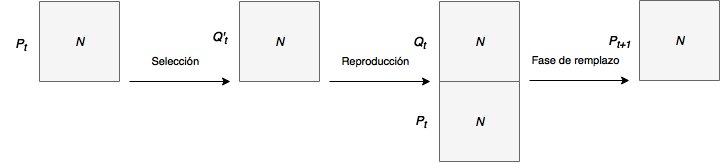
\includegraphics[scale=0.5]
{Figures_Chapter3/Evolution_Process.png}
\decoRule
\caption{Proceso para seleccionar una población $P_{t+1}$ y generar una población nueva $Q_{t+1}$  en cada generación.}
\label{fig:Proceso_Generacion}
\end{figure}
%


\subsection*{Fase de remplazo}

En este proceso de selección, se considera la diversidad en el espacio de las variables y el espacio objetivo simultáneamente.
%
Particularmente, en base al criterio de paro, en las primeras etapas se induce un mayor grado de exploración en el espacio de las variables, y conforme transcurre la ejecución, la diversidad en el espacio de las variables es decrementada gradualmente, transformándose así en un esquema más tradicional, donde se desea obtener soluciones próximas y diversas al frente de Pareto.
%
De esta forma, se promueve una apropiada exploración y se evita converger prematuramente a ciertas regiones, lo cual es especialmente importante en el caso de ejecuciones a largo plazo, que es el ámbito en el que los métodos que incorporan un control especial de diversidad en el espacio de las variables reportan mayores beneficios.
%
La estrategia para inducir la diversidad consiste en penalizaciones, similar al utilizado en \cite{Joel:ANovelDiversityBasedEAForTheTSP} para el caso de optimización mono-objetivo.
%
Así, en la fase de remplazo a partir de $2N$ individuos, donde $N$ corresponden a los individuos padres ($P_t$) y $N$ a los hijos ($Q_t$), se eligen $N$ individuos para sobrevivir, convirtiéndose en los individuos padre de la siguiente generación ($P_{t+1}$), como se observa en la parte izquierda de la figura \ref{fig:Proceso_Generacion}.
%

La idea base, consiste en que después de seleccionar un individuo el cual es utilizado como referencia, y en base a una métrica de distancia\footnote{En dominios continuos se implementa la distancia Euclídea}, se sitúa una hiperesfera de tamaño $D$ centrada en el individuo de referencia, y se desea evitar que cualquier individuo que esté dentro de la hiperesfera sea seleccionado.

La fase de remplazo se describe en el Algoritmo \ref{alg:Fase_Remplazo}, donde en cada generación se calcula un valor $D$ que como ya se mencionó es utilizado para definir el radio de las hiperesferas. 
%
Este valor es calculado en la línea \ref{DInicial}, teniendo en cuenta el número de generaciones transcurridas ($G_{Transcurridas}$) y el número de generaciones a ejecutar ($G_{Final}$).
%
En el conjunto $R_t$ se incluyen todos los individuos que son candidatos para ser seleccionados, además inicialmente no existen individuos penalizados (línea \ref{alg:Fase_Remplazo:Penalizados_Vacios}).
%
En cada generación, específicamente en la fase de remplazo, se introduce en el conjunto de referencia ($P_{t+1}$) los individuos extremos del conjunto $R_t$ que está conformado por la unión entre los individuos padres e hijos (línea \ref{alg:Fase_Remplazo:Extremos}), así son seleccionados $M$ individuos ($M$ objetivos) los cuales tienen la mejor aptitud en cada objetivo de forma independiente, por ejemplo para el caso de dos objetivos en la figura \ref{fig:Extremos_Seleccionados} los individuos extremos están indicados de color rojo.

\begin{figure}[H]
\centering
\scriptsize
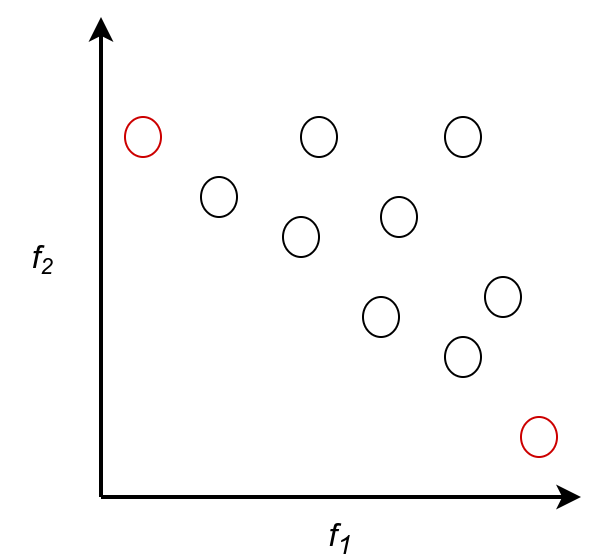
\includegraphics[scale=0.2]
{Figures_Chapter3/Extremos_Seleccionados.png}
\decoRule
\caption{Soluciones que corresponden a los extremos en dos objetivos.}
\label{fig:Extremos_Seleccionados}
\end{figure}

%
Posteriormente hasta obtener $N$ individuos ($P_{t+1}$) se realizan los siguientes pasos (líneas \ref{alg:Calculo_Diversidad_Primero} - \ref{alg:Fase_Remplazo:seleccionarobj}).
%
Primeramente se calcula la diversidad en el espacio de las variables de cada individuo candidato (línea \ref{alg:Calculo_Diversidad_Primero}), tomando a los individuos seleccionados como referencia.
%
Los individuos que se encuentren demasiado cercanos a cualquier individuo de referencia, son transferidos al conjunto de individuos penalizados (línea \ref{alg:Calculo_Diversidad_Primero_Move}).
%

Después de tratar la diversidad en el espacio de las variables y sólo considerando a los individuos que son candidatos, identificados también como los individuos no penalizados, el proceso de selección es enfocado en el espacio objetivo, donde para seleccionar a los siguientes individuos, en cada paso se calcula el rango de dominancia propuesto por \citeauthor{Joel:NSGAII} en \cite{Joel:NSGAII}, este procedimiento considera a los individuos de referencia junto a los individuos candidatos (línea \ref{alg:fast_non_dom}).
%
A continuación se elige al candidato que tiene el mínimo rango, y en caso de empate, al que ofrezca mejor diversidad en el espacio objetivo (línea \ref{alg:Fase_Remplazo:seleccionarobj}).
%
En la figura \ref{fig:Rangos} se presenta un ejemplo en el caso de dos objetivos, donde los círculos con borde de color rojo representan a los individuos de referencia o ya seleccionados y con bordes de color verde a los individuos candidatos.
%

\begin{figure}[H]
\centering
\scriptsize
%\includegraphics[width=6cm, height=6cm]
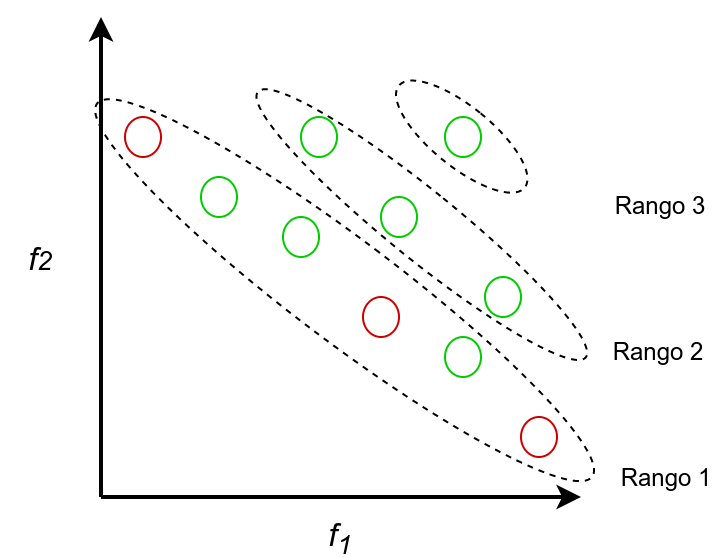
\includegraphics[scale=0.2]
{Figures_Chapter3/Rangos.png}
\decoRule
\caption{Clasificación de rangos con los individuos de referencia en color rojo y los  candidatos de color verde.}
\label{fig:Rangos}
\end{figure}

En caso que todos los individuos estén penalizados (línea \ref{alg:Fase_Remplazo:Vacio}), se elige al que tenga una mayor contribución a la diversidad en el espacio de las variables, es decir, aquel que esté mas alejado a los individuos de referencia (líneas \ref{alg:Calculo_Diversidad_Penalizados}-\ref{alg:Distante_Variables}).
%
Entonces el efecto del parámetro $D$ define el grado de diversidad, así si se utilizan hiperesferas más grandes, se inducen mayores grados de diversidad.

%
Para relacionar el principio de diversidad con el criterio de paro, el radio que corresponde a la hiperesfera comienza con un valor inicial $D_i$, y posteriormente éste va decrementándose linealmente conforme avanza la ejecución del algoritmo.
%
El modelo para modificar el radio de la hiperesfera es decrementado linealmente hasta el valor cero cuando han transcurrido la mitad de generaciones, lo que permite que el método se transforme en un MOEA tradicional en el que no se considera la diversidad en el espacio de las variables, ya que no se producirán penalizaciones.
%

\begin{algorithm}[H]
\algsetup{linenosize=\tiny}
  \scriptsize
	\caption{Fase de remplazo del VSD-MOEA} 
	\begin{algorithmic}[1]
    	\STATE Entrada: $P_t$ (Población de la generación actual), $Q_t$ ( Población hijo de la generación actual)
    	\STATE Salida: $P_{t+1}$
		\STATE $D = D_I - D_I *2* \frac{G_{Transcurridas}}{G_{Final}}$ \label{DInicial}			
        \label{Modelo}
        \STATE $P_{t+1} = \emptyset$
        \STATE $R_t = P_t \cup Q_t$ \label{alg:Fase_Remplazo:Inicio_Rt}
         \STATE $Penalizados = \emptyset$ \label{alg:Fase_Remplazo:Penalizados_Vacios}
		\STATE mover( $R_t$,  $P_{t+1}$, Los mejores en cada objetivo) \label{alg:Fase_Remplazo:Extremos}
        \label{alg:Extremos}
        \WHILE{ $|P_t|$ $\leq$ N } \label{alg:Fase_Remplazo:ciclo}
			\STATE Calcular \textbf{Diversidad\_Espacio\_Variables} ($R_t$, $P_{t+1}$) \label{alg:Calculo_Diversidad_Primero}
		\STATE mover($R_t$, Penalizados, Diversidad en el espacio de las variables $ < $ D)  \label{alg:Calculo_Diversidad_Primero_Move}
        \IF{$R_t$ está vacío} \label{alg:Fase_Remplazo:Vacio}
				\STATE Calcular \textbf{Diversidad\_Espacio\_Variables} ($Penalizados$, $P_{t+1}$) \label{alg:Calculo_Diversidad_Penalizados}
				\STATE mover(Penalizados, $R_t$, Más alejado en el espacio de las variables) \label{alg:Distante_Variables}
        \ENDIF
		\STATE $ordenaci \acute{o} n-eficiente-basado-no-dominados(R_t \cup P_{t+1}) $ \label{alg:fast_non_dom}
		\STATE Calcular \textbf{Diversidad\_Espacio\_Objetivo}($R_t$, $P_{t+1})$) \label{alg:Diversidad_Espacio_Objetivo}
        \STATE mover($R_t$, $P_{t+1}$, Menor rango en caso de empate seleccionar al más alejado en el espacio objetivo)  \label{alg:Fase_Remplazo:seleccionarobj}
        \ENDWHILE
	\RETURN $P_{t+1}$
	\end{algorithmic}
    \label{alg:Fase_Remplazo}
\end{algorithm}

\subsection*{Proceso empírico de la fase de remplazo}

En esta sección se explica de forma empírica un parte de la fase de remplazo que corresponde, la cual corresponde al escenario ilustrado en la figura \ref{fig:Simulacion_1} donde se muestran ocho individuos ubicados en el espacio de las variables y en el espacio objetivo respectivamente, los individuos de referencia estan indicados con un borde de color rojo, el conjunto de indiviuos hijos y padres respectivamente son $Q_t = \{1,2,3,4\}$, $P_{t} = \{5,6,7,8\}$, el número de individuos a seleccionar son $N=4$. 
%
Al inicio $R_t = \{1, 2, 3, 4, 5, 6, 7, 8 \}$, donde los individuos extremos $\{1, 2\}$ son trasladados a $P_{t+1}$.
%
\begin{figure}[H]
\centering
\scriptsize
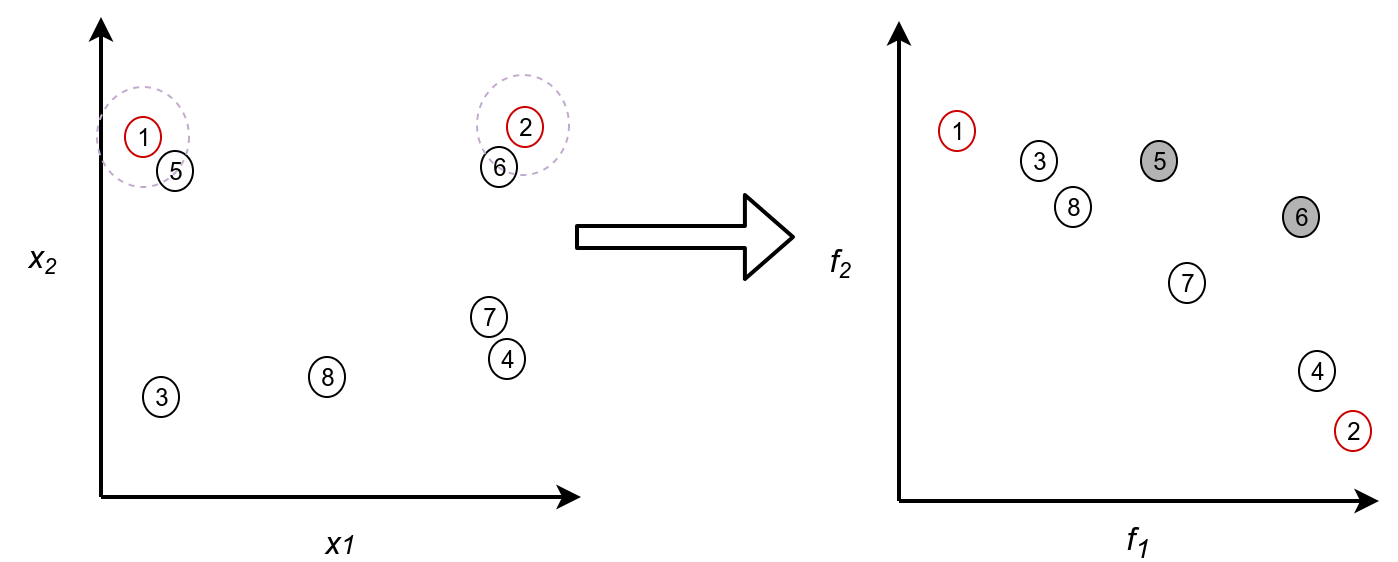
\includegraphics[scale=0.2]
{Figures_Chapter3/Fase_Remplazo_1.png}
\decoRule
\caption{Simulación de la fase de remplazo, en la parte izquierda están los individuos en el espacio de las variables y en la parte de la derecha el espacio objetivo.}
\label{fig:Simulacion_1}
\end{figure}


Se puede observar que en la primer iteración en el espacio de las variables se traza un hiperesfera de color gris en cada uno de los individuos de referencia ($\{1, 2\}$) donde los individuos $5$ y $6$ se ubican dentro de la hiperesfera de cada uno de los individuos de referencia por lo que son movidos al conjunto de penalizados que son identificados con fondo de color gris en el espacio objetivo.
%

Después de considerar el espacio de las variables, se selecciona al mejor individuo en el espacio objetivo, donde se debe implementar una clasificación por rangos.
%
Se aclara que los individuos $\{5, 6\}$ no se consideran en la clasificación por rangos ya que están penalizados.
%
Entonces en este caso el primer rango está conformado por los individuos $r_1 = \{1, 3, 8, 7, 4, 2 \}$, por lo tanto el conjunto de candidatos no penalizados es $R_t = \{3,4,7,8\}$.
%
Entonces se debe realizar el cálculo de la diversidad en el espacio objetivo, ya que todos los candidatos pertenecen al menor rango.
%
El individuo con etiqueta $7$ es seleccionado ya que contribuye más a la diversidad en el espacio objetivo, así los individuos de referencia en la siguiente iteración son $P_{t+1} = \{1, 2, 7\}$, como se observa en la figura \ref{fig:Simulacion_2}.
%
\begin{figure}[H]
\centering
\scriptsize
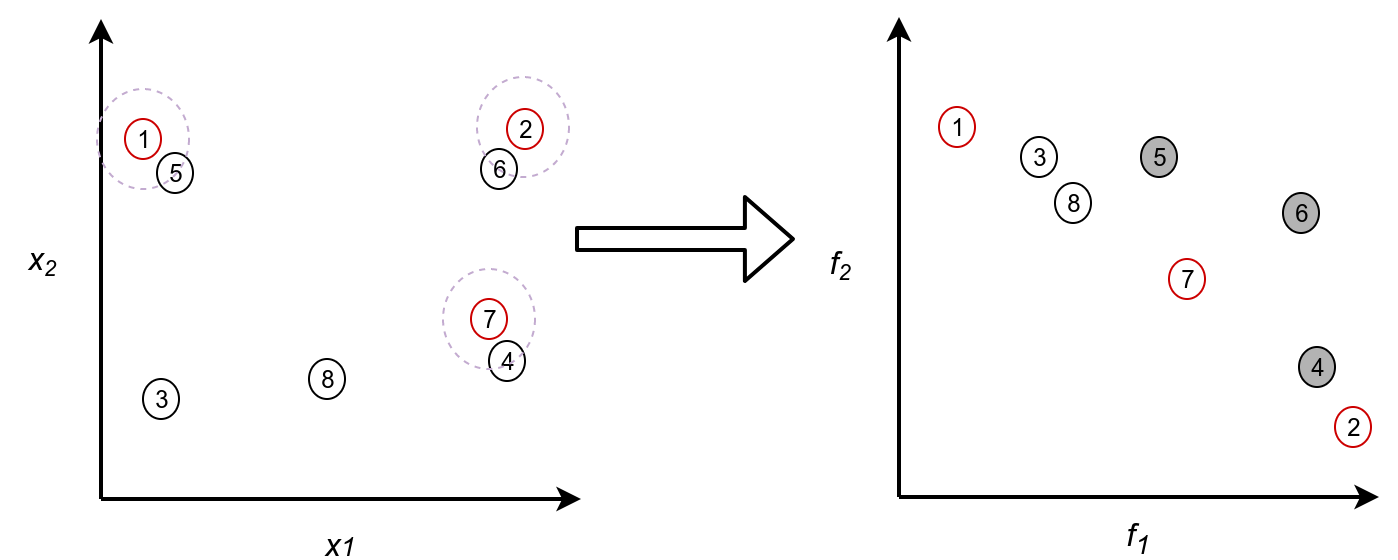
\includegraphics[scale=0.2]
{Figures_Chapter3/Fase_Remplazo_2.png}
\decoRule
\caption{Simulación de la fase de remplazo, en la parte izquierda están los individuos en el espacio de las variables y en la parte de la derecha el espacio objetivo.}
\label{fig:Simulacion_2}
\end{figure}

Posteriormente para seleccionar al siguiente individuo, se realiza el mismo procedimiento pero ahora considerando al individuo $7$ como referencia, que al ser agregado tiene un efecto en el espacio de las variables, ya que podría ocasionar que más individuos estén penalizados, en este caso como resultado de seleccionar al individuo con etiqueta $7$ se penaliza al individuo con etiqueta $4$, el cual ya no será considerado en la clasificación de rangos.
%

Ahora los individuos candidatos son $R_t = \{3, 8\}$, los cuales pertenecen al menor rango por lo que es necesario considerar su contribución en la diversidad del espacio objetivo, siendo el mejor candidato el individuo con etiqueta $8$, el cual es seleccionado y movido al conjunto de referencia $P_{t+1} = \{1, 8 ,7, 2\}$.
%
El proceso termina ya que los $N$ individuos fueron seleccionados, terminando la simulación como se muestra en la figura \ref{fig:Simulacion_3}.

\begin{figure}[H]
\centering
\scriptsize
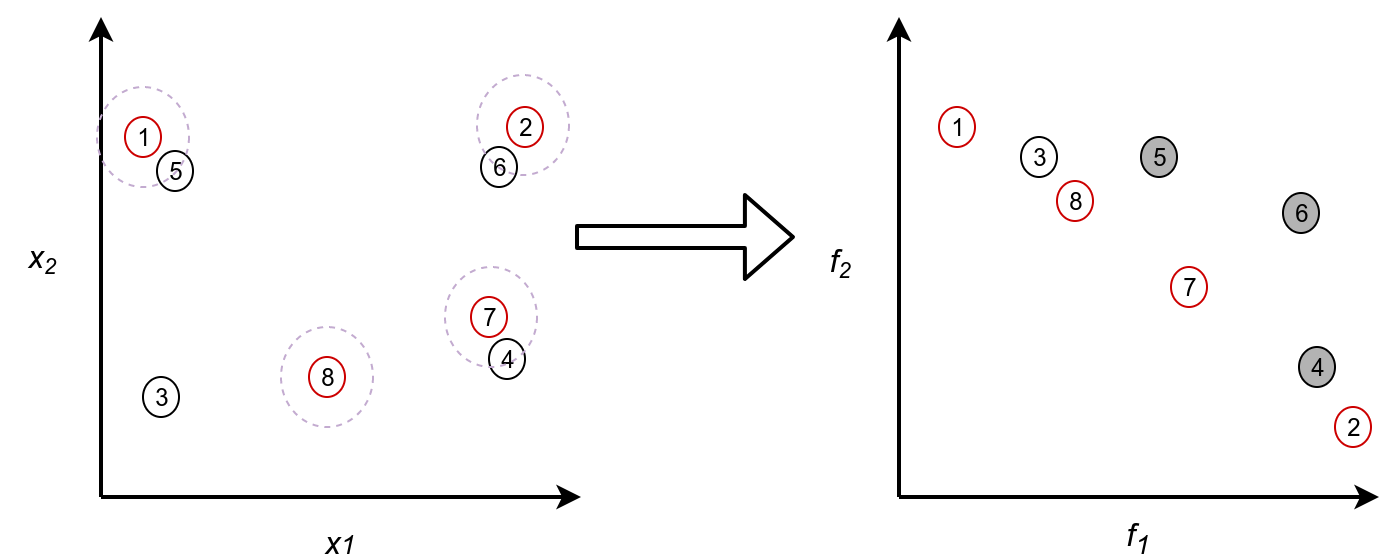
\includegraphics[scale=0.2]
{Figures_Chapter3/Fase_Remplazo_3.png}
\decoRule
\caption{Simulación de la fase de remplazo, en la parte izquierda están los individuos en el espacio de las variables y en la parte de la derecha el espacio objetivo.}
\label{fig:Simulacion_3}
\end{figure}
%
Se observa que si el radio de la hiperesfera es cero o muy pequeño, el comportamiento del algoritmo es similar a los esquemas tradicionales (\cite{Joel:NSGAII}).
%
El efecto de asignar el radio de la hiperesfera con un valor mayor al espacio de las variables produce un grado elevado de exploración.
%
Si este valor fuera muy elevado inicialmente se ubicarían a todos los individuos candidatos en el conjunto de penalizados, seleccionando así al individuo que tiene mayor contribución a la diversidad en el espacio de las variables, que como se muestra en la figura \ref{fig:Simulacion_Penalizados}, al inicio de esta simulación el individuo seleccionado sería el $8$ en lugar del $7$ como se analizó anteriormente.
\begin{figure}[H]
\centering
\scriptsize
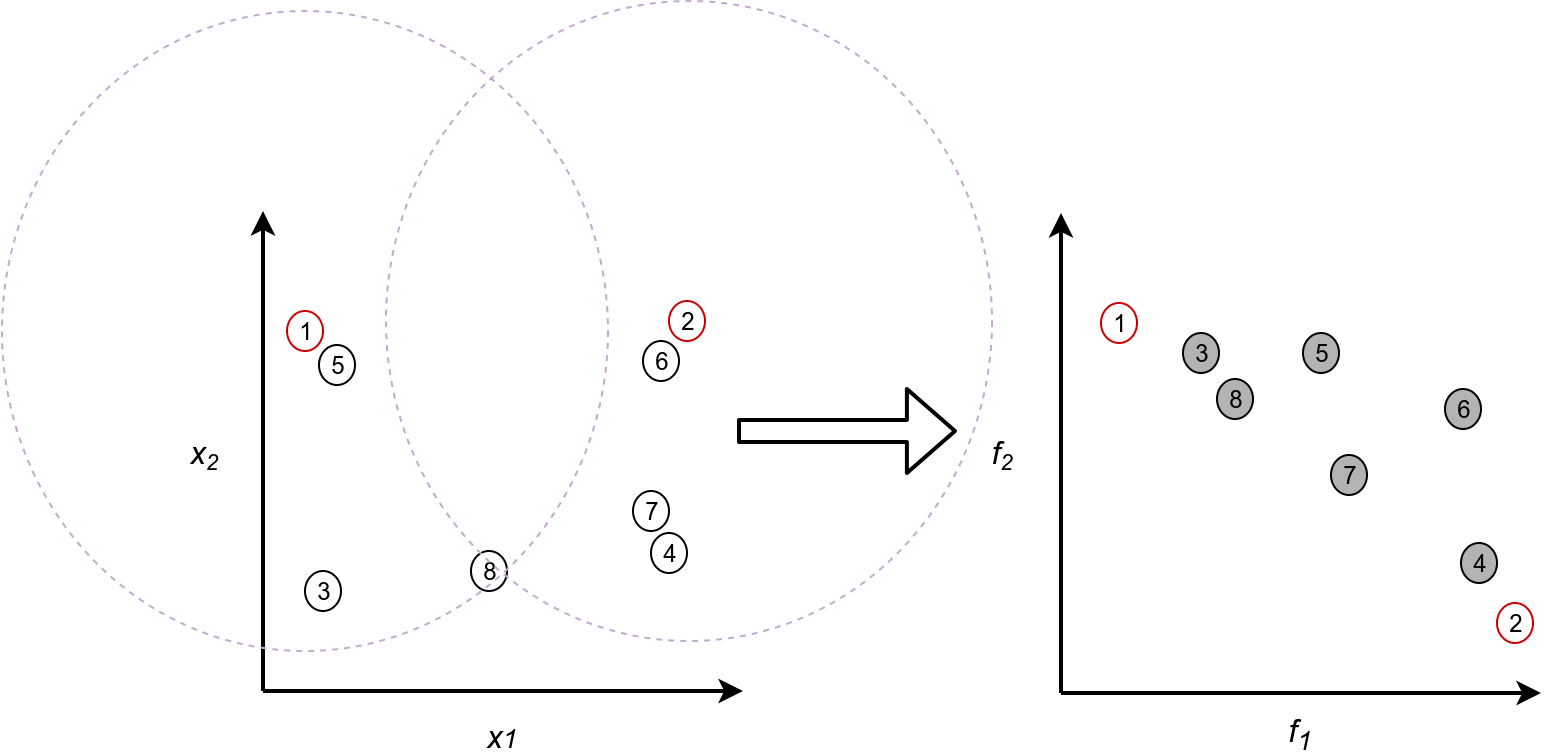
\includegraphics[scale=0.2]
{Figures_Chapter3/Fase_Remplazo_Penalizados.png}
\decoRule
\caption{Asociación de cada individuo candiato con su individuos de referencia más cercano.}
\label{fig:Simulacion_Penalizados}
\end{figure}

\subsection*{Diversidad en el espacio objetivo}

Al final de la fase de remplazo se realiza la selección del individuo con menor rango, en caso de que existan varios individuos candidatos, se elige al que contribuye más a la diversidad en el espacio objetivo.
%
Se puede implementar cualquier método para cuantificar la contribución de cada individuo a la diversidad, inclusive se podría aplicar algún indicador que ofrezca soluciones bien distribuidas y próximas al frente de Pareto.
%

Uno de los métodos más utilizados en los MOEAs basados en dominancia es denominado como distancia de amontonamiento, y consiste en eliminar iterativamente a cada individo con la mínima contribución a la diversidad (\cite{Joel:NSGAII}), donde la contribución de cada individuo es calculada en base a la distancia al vecino más cercano.
%
Este procedimiento está íntimamente relacionado con el análisis de clústering, específicamente al modelo de conectividad o jerárquico, en particular este método es de la categoría \textit{divisible}, donde todas las observaciones inician como parte del mismo clúster, y después mediante un criterio es seleccionado un clúster y es dividido en dos, esto se realiza de forma recursiva, también puede ser considerado como un enfoque \textit{top down}.
%

El método que se propone es clasificado como \textit{aglomerativo}, donde cada observación es considerada como un clúster, e iterativamente mediante una regla establecida, los pares de clústers son combinados, así considerado como un enfoque \textit{bottom up}.

%
Una regla para combinar dos clústers, consiste en seleccionar al par con la mínima distancia de cercanía, esta distancia de cercanía puede ser definida como la mínima distancia euclídea\footnote{Este problema es popular conocido como "Nearest-Neighbor".} entre cualquier par de puntos, cada uno escogido de su respectivo clúster como es definido por \citeauthor{Joel:leskovec2014mining} en \citetitle{Joel:leskovec2014mining}.
%

En esta implementación se propone una variante que consiste en seleccionar al individuo candidato con la máxima distancia de cercanía, con el propósito de promover la diversidad en el espacio objetivo.
%
Entonces, se define que los individuos de referencia ($P_{t+1}$) son representados por un clúster y cada individuo candidato ($R_t$) como otro clúster como se muestra en la figura \ref{fig:Clusters}, así la regla para combinar los clústers es modificada de tal forma que el individuo candidato que tenga mayor aportación a la diversidad sea seleccionado y sea combinado con el clúster que correponde a los individuos de referencia.
\begin{figure}[H]
\centering
\scriptsize
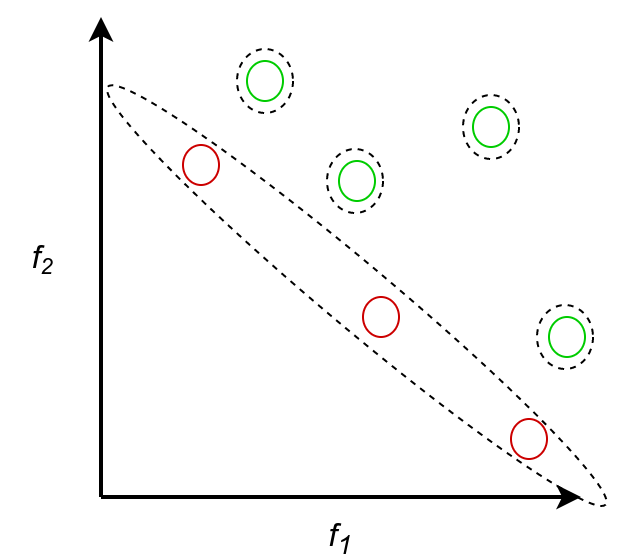
\includegraphics[scale=0.2]
{Figures_Chapter3/Cluster.png}
\decoRule
\caption{Los individuos de referencia con borde rojo representan un cluster y los candidatos con borde verde representan un cluster cada uno.}
\label{fig:Clusters}
\end{figure}

%
Además es necesario agregar una restricción en donde los individuos candidatos no se pueden unir entre ellos.

%
Por lo tanto, el proceso para seleccionar a un individuo candidato, consiste en asociar a cada individuo candidato con el vecino más cercano de los individuos de referencia.
%
Así el candidato seleccionado, será el que tenga mayor distancia de cercania a su respectivo individuo de referencia, como se muestra en la figura \ref{fig:Distancia_Cercania}, donde los círculos con borde de color rojo corresponden a los individuos de referencia y los de color verde a los individuos candidatos, se observa que cada candidato es asociado al individuo de referencia más cercano.
%
Específicamente en este caso el candidato con etiqueta $7$ es el que tiene mayor distancia de cercanía a su individuo de referencia asociado con etiqueta $2$.
%

\begin{figure}[H]
\centering
\scriptsize
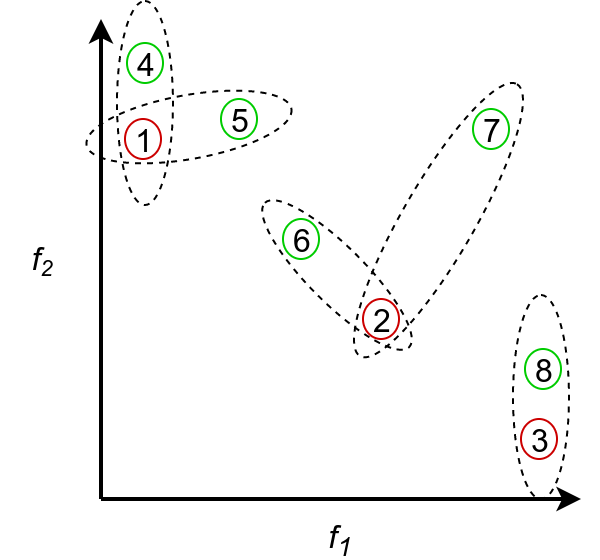
\includegraphics[scale=0.2]
{Figures_Chapter3/Distancia_Cercania.png}
\decoRule
\caption{Simulación de la fase de remplazo, al asignar un valor elevado al radio de la hiperesfera.}
\label{fig:Distancia_Cercania}
\end{figure}

Este proceso de selección promueve convergencia ya que inicialmente en cada fase de remplazo son seleccionados los individuos extremos, y posteriormente se obtiene diversidad al escoger al candidato con la máxima distancia de cercanía, además se considera el proceso de clasificación por rangos.
%

El proceso para seleccionar al individuo con mayor distancia de cercanía está definido en el algoritmo \ref{alg:Diversidad_Espacio_Objetivo}, donde se calcula la menor distancia euclídea entre $R_t$ y $P_{t+1}$, así  de forma iterativa se almacena la mayor distancia euclídea entre estos dos conjuntos ya definida como la distancia de cercanía, por último el procedimiento regresa al individuo el cual tiene mayor distancia de cercanía a su individuo de referencia asociado.


\begin{algorithm}[H]
\scriptsize
	\caption{Diversidad\_Espacio\_Objetivo} 
	\label{alg:Diversidad_Espacio_Objetivo}
	\begin{algorithmic}[1] 
	\STATE Entrada: $R_t$ (Soluciones disponibles), $P_{t+1}$ (Soluciones seleccionadas)
	\FOR{$r \in R_t$}
	   \STATE Maxima\_Distancia = $-\infty$
	   \FOR{$p \in P_{t+1}$}
		\STATE $D_{r,p} = \sqrt{ \sum_{ m \in M} (r.obj[m] -  p.obj[m])^2  }$
		\STATE Distancia\_Proximidad= minimo(MaxDist, $D_{r,p}$)
	   \ENDFOR
	   \IF{ Distancia\_Proximidad > Maxima\_Distancia  }
		\STATE Maxima\_Distancia = Distancia\_Proximidad
		\STATE Seleccionado = $r$
	   \ENDIF
	\ENDFOR
	\RETURN Seleccionado
	\end{algorithmic}
\end{algorithm}

%Aunque este principio es ideal para seleccionar al mejor individuo en el espacio objetivo, no es posible obtener una distribución de puntos totalmente equiespaciados con el frente de Pareto, ya que en teoría es necesario tener $2^i + 1$ puntos.
%
%Esto se puede visualizar considerando un caso sencillo, en una dimensión donde se tiene una recta representando el conjunto de soluciones optimas compuestas, en el procedimiento establecido anteriormente primero se seleccionan las soluciones de los extremas, posteriormente el punto óptimo con mayor distancia de cercanía corresponderá al centro de la recta.
%
%Hasta este punto se observa que los puntos están adecuadamente distribuídos, pero ahora al seleccionar el siguiente punto, se observa se ubicará entre un punto extremo y el centro, pero al ubicar este punto en uno de los dos espacios se tendrá un espacio mayor al resto de espacios.
%

%
%Conforme el número de puntos aumenta la distribución de los puntos es menos afectado, inclusive en la práctca existen problemas en el rendimiento de un MOEA.
%
%Aunque la distancia de cercanía parece ideal, existe un inconveniente al aumentar el número de objetivos, ya que en dos objetivos el concepto de dominancia asegura que seleccionar al individuo más lejano nunca afecatará la convergencia.
%


Se destaca que seleccionar al candidato con la máxima distancia de cercanía es teóricamente correcto para el caso de dos objetivos ya que al implementar la clasificación por rangos se asegura un grado de convergencia.
%
No obstante pueden existir problemas de convergencia en más de dos objetivos como es el caso de problemas multi-frontales, esto surge por la definición de dominancia, donde la capacidad de búsqueda es deteriorada severamente (\cite{Joel:MOEA_Survey}).
%
Una idea sencilla para mejorar la escalbilidad de un MOEA basado en dominancia es incrementar la presión de selección hacia el frente de Pareto.
%
Así, un enfoque basado en esta idea es mediante la modificación de la dominancia de Pareto para decrementar el número de soluciones no dominadas en cada población (\cite{Joel:Dominance_Area}).
%
Otra alternativa se basa en asignar diferentes rangos a las soluciones que son no dominadas (\cite{Joel:MOEA_Optimisation_Based_on_Relation_Favour, Joel:Ranking_Dominance_And_Many_Objective_Optimization}).
%

También se han propuesto métodos suplementarios para obtener la contribución de diversidad en problemas de muchos objetivos (\cite{Joel:Substitute_Distance_Assignments_in_NSGA_II_Many_Objective_Problems}), estos son:
\begin{itemize}
\item Sub-vector de dominancia (SV-DOM).
\item Dominancia epsilon ($\epsilon$-DOM).
\item Dominancia de Pareto difusa.
\item Cuenta de dominancia en sub-objetivos.

\end{itemize}


Una propuesta que no requiere de muchos cambios considerando el método previamente mencionado, consiste en utilizar el mismo procedimiento de asociación, adicionalmente se emplea una distancia distinta donde sólo es cuantificada la mejoría en cada objetivo entre los individuos candidatos con los individuos de referencia, además esta distancia es considerada en la distancia generacional invertida modificada IGD+ (\cite{Joel:IGDPlus_And_GDPlus}), la cual es conocida como débilmente Pareto \textit{Compliant}.
%
Así esta distancia es definida como \textit{distancia de mejoría} ($D^b(p_i, r_i)$):
\begin{equation}
   \begin{split}
	D^b(p_i, r_i) = \sum_{i \in M} d_i^2 \\
	s.a. \quad d_i = max\{0, p_i - r_i\}
   \end{split}
\end{equation}
donde $p_i$ es un individuo que pertenece a los seleccionados o de referencia $P_{t+1}$, y por otra parte $r_i$ pertenece a los individuos candidatos $R_t$.
%

Es de esperarse que la distancia no cumpla la desigualdad del triángulo siendo una propiedad importante indicado por \citeauthor{Joel:HausdorffDistance} en \citetitle{Joel:HausdorffDistance}, puesto que la noción de dominancia tampoco cumple esta propiedad.
%
Además la distancia de mejoría sitúa las soluciones en el espacio de los objetivos bajo el principio de dominancia, teniendo un efecto similar a algúnos MOEAs que son guiados por el hipervolúmen.
%

Para verificar el efecto que existe al implementar la distanca de mejoría, de forma empírica se aplica la selección dada una muestra de puntos evaluadas en la función que corresponde a una esfera, el proceso consiste en generar $20000$ puntos mediante una distribución uniforme en cada una de las tres variables $x_1$, $x_2$ y $x_3$ $~U[0,1]$, posteriormente estos puntos son evaluados en cada objetivo.
%
Consecuentemente, se realiza la selección de $200$ puntos como es indicado en el algoritmo \ref{alg:Diversidad_Espacio_Objetivo}, este procedimiento se aplicó dos veces uno con cada distancia.
%
En la figura \ref{fig:Distancia_Mejoria} se pueden observar los puntos seleccionados al implementar cada distancia.
%
Aunque la distancia Euclídea visualmente distribuye mejor los puntos en el espacio, esta métrica presenta dificultades al aumentar los objetivos.
%
Por otra parte la distancia de mejoría tiene el efecto de seleccionar los puntos en ciertas regiones que son más significativas en el espacio objetivo, por lo tanto se puede observar que las regiones planas de la figura carecen de puntos, particularmente este es el efecto que se obtiene al guiar el proceso de búsqueda por medio del hipervolumen.

\begin{figure}[H]
\centering
\scriptsize
\includegraphics[scale=0.23,angle=-90,origin=c]
{Figures_Chapter3/euclidea.eps}
\includegraphics[scale=0.23, angle=-90,origin=c]
{Figures_Chapter3/mejoria.eps}
\caption{Proceso de selección utilizando la distancia Euclídea en la parte izquierda y la distancia de mejoría en la parte derecha.}
\label{fig:Distancia_Mejoria}
\end{figure}

\section{Simulación Algoritmo VSD-MOEA}

En optimización estocástica los problemas de prueba surgen con el propósito de cualificar las propiedades de cada algoritmo.
%
Por otra parte, los algoritmos basados en diversidad promueven soluciones de calidad y ofrecen estabilidad en ejecuciones a largo plazo, así un algoritmo basado en diversidad tiene una mayor posibilidad de aproximar apropiadamente a la solución o conjunto de soluciones óptimas.
%
En el caso mono-objetivo se ha probado que este tipo de algoritmos ofrecen mejores resultados en instancias que son consideradas más difíciles como es mostrado por \citeauthor{Joel:Dynamic_FAP} en \citetitle{Joel:Dynamic_FAP}.
%

En los primeros algoritmos genéticos cada individuo estaba representado por una forma binaria conocido como \textit{genotipo}, de modo que se basan en esquemas de bajo orden y arriba del promedio, esto para formar bloques constructores de mayor orden (\cite{goldberg1987genetic}).
%
En base a esto se diseñó una clase de funciones \textit{Funciones deceptivas para algoritmos genéticos} donde en promedio los bloques constructores\footnote{Un bloque constructor es un esquema basado en el genotipo de la población } de bajo orden son engañados, por lo tanto usualmente no son combinados los bloques constructores de mayor orden. En el caso extremo, hay funciones enteramente deceptivas donde todos los esquemas de bajo orden contienen una solución sub-óptima que son mejores que otros esquemas que compitieron en el proceso (\cite{deb1993analyzing}).
%
Esto quiere decir que las funciones deceptivas introducen una forma en como los algoritmos genéticos se comportan de tal manera que el espacio de búsqueda pueda proporcionar una presión de selección para el algoritmo en ubicar individuos en direcciones erróneas.
%
%
Actualmente, los algoritmos genéticos en dominios continuos están representados por números reales, por lo tanto se han adaptado las funciones deceptivas en codificación real.

A continuación se presenta una simulación del algoritmo propuesto y el estado del arte de MOEAs, particularmente se considera la instancia de prueba WFG5, la cual implementa una transformación deceptiva.
%
Por lo tanto en la figura \ref{fig:Forma_Deceptiva} se muestra un ejemplo de una función deceptiva en dominios continuos y en el caso mono-objetivo.
%
Principalmente se puede observar que pueden ser encontrados fácilmente las zonas que corresponden a los mínimos locales.
%
Sin embargo, la región que corresponde al mínimo global es muy estrecha, por lo tanto es complicado que el EA sitúe individuos en esa zona de búsqueda.
%



\begin{figure}[H]
\centering
\scriptsize
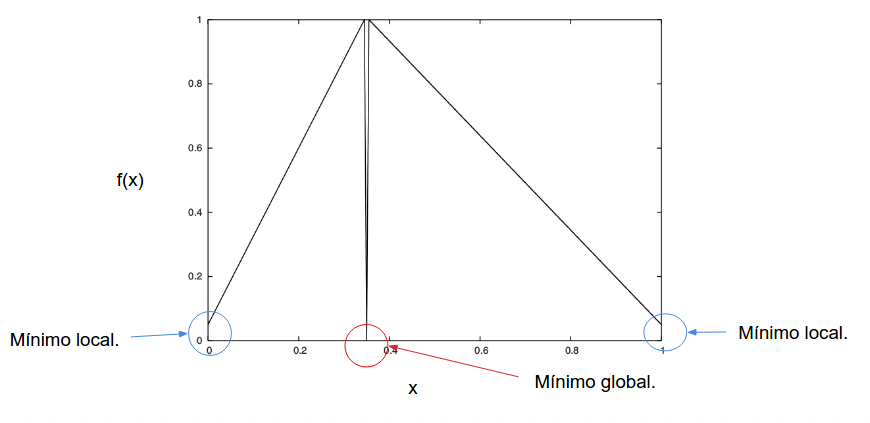
\includegraphics[scale=0.3]
{Figures_Chapter3/Forma_Deceptiva.png}
\decoRule
\caption{Forma de una función deceptiva en dominios continuos.}
\label{fig:Forma_Deceptiva}
\end{figure}

Específicamente, se consideran mil generaciones, además se toman en cuenta dos variables de decisión y dos funciones objetivo, como es mostrado en la figura \ref{fig:Simulacion_Algoritmo_1}, en la parte izquierda está representado el espacio objetivo y en la derecha el espacio de las variables.
%
Además, en el espacio de las variables, las regiones que corresponden a los óptimos locales están ubicados en los extremos (color azul) y el óptimo global pertence a una línea situada en el centro (color rojo), por lo tanto existe una mayor probabilidad de asignar individuos en las regiones que corresponden a los óptimos locales.
%
Se observa que conforme transcurren las generaciones los algoritmos del estado del arte ubican soluciones en los óptimos locales, particularmente al 1\% del total de generaciones (generación 10) los algoritmos MOEA/D, NSGA-II y el GDE3 se aproximaron a los óptimos locales.
%
Mientras que los algoritmo MOMBI-II, SMS-EMOA y VSD-MOEA, todavía mantienen individuos diversos.
%
Particularmente, el MOMBI-II utiliza un proceso adaptativo por lo tanto hasta este momento mantiene individuos diversos.
%
Por otra parte el SMS-EMOA remplaza únicamente a un individuo en cada generación, por lo tanto la convergencia es retrasada en comparación a los demás MOEAs. 
%

Posteriormente al 40\% de las generaciones (figura \ref{fig:Simulacion_Algoritmo_4}), los algoritmos que pertenecen al estado del arte ubicaron soluciones en las regiones que corresponden a los óptimos locales, por otra parte el VSD-EMOA mantiene una cantidad de soluciones en el óptimo global, y otra cantidad de individuos están dispersos en el espacio de las variables.
%
Al finalizar la ejecución, el VSD-MOEA es el único algoritmo que sitúa las soluciones en la región de óptimos globales, hasta este punto los algoritmos que pertenecen al estado del arte difícilmente podrían ubicar soluciones en la región óptima global, aún así existe una probabilidad mínima de ubicar un individuo por medio de los operadores evolutivos.

\begin{figure}[H]
\centering
\scriptsize
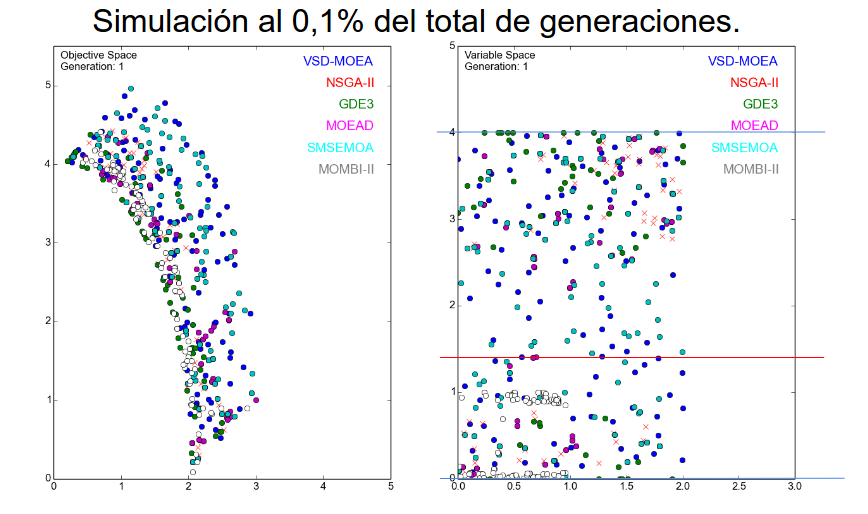
\includegraphics[scale=0.35]
{Figures_Chapter3/Simulacion_Algoritmo_1.png}
\decoRule
\caption{Simulación de la fase de remplazo, al asignar un valor elevado al radio de la hiperesfera.}
\label{fig:Simulacion_Algoritmo_1}
\end{figure}


\begin{figure}[H]
\centering
\scriptsize
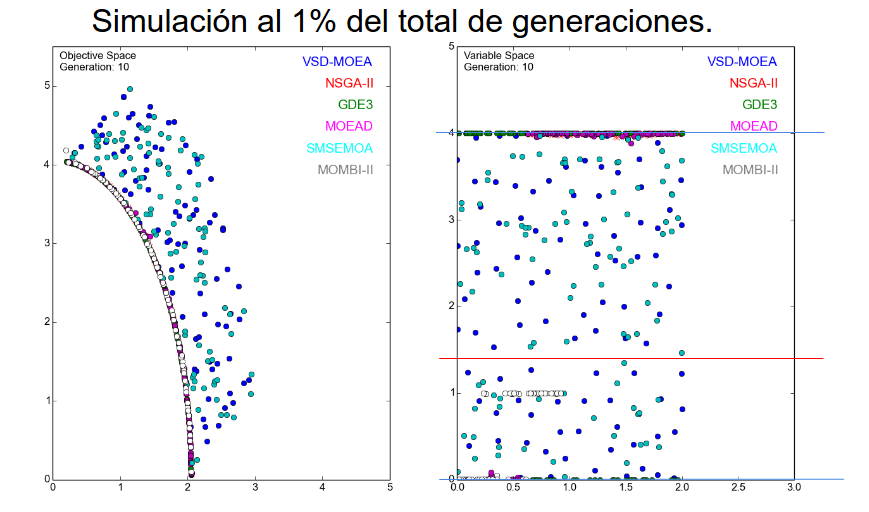
\includegraphics[scale=0.35]
{Figures_Chapter3/Simulacion_Algoritmo_2.png}
\decoRule
\caption{Simulación de la fase de remplazo, al asignar un valor elevado al radio de la hiperesfera.}
\label{fig:Simulacion_Algoritmo_2}
\end{figure}

%\begin{figure}[H]
%\centering
%\scriptsize
%\includegraphics[scale=0.4]
%{Figures_Chapter3/Simulacion_Algoritmo_3.png}
%\decoRule
%\caption{Simulación de la fase de remplazo, al asignar un valor elevado al radio de la hiperesfera.}
%\label{fig:Simulacion_Algoritmo_3}
%\end{figure}

\begin{figure}[H]
\centering
\scriptsize
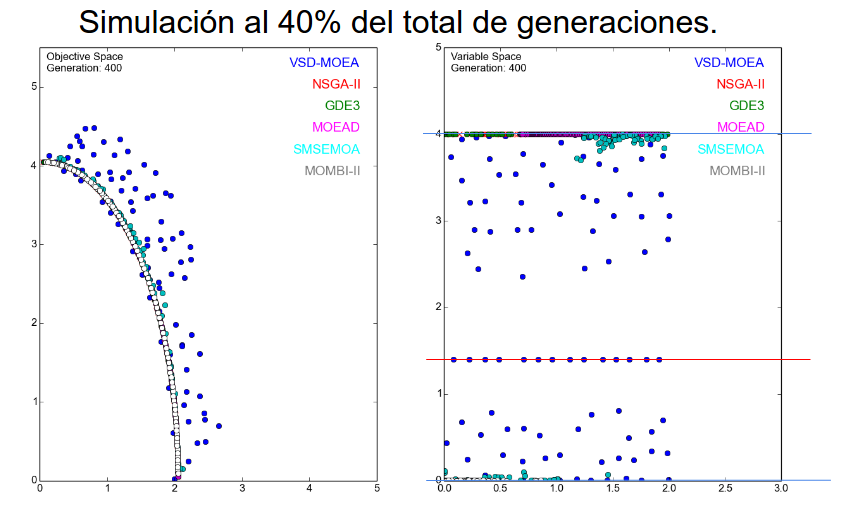
\includegraphics[scale=0.35]
{Figures_Chapter3/Simulacion_Algoritmo_4.png}
\decoRule
\caption{Simulación de la fase de remplazo, al asignar un valor elevado al radio de la hiperesfera.}
\label{fig:Simulacion_Algoritmo_4}
\end{figure}

\begin{figure}[H]
\centering
\scriptsize
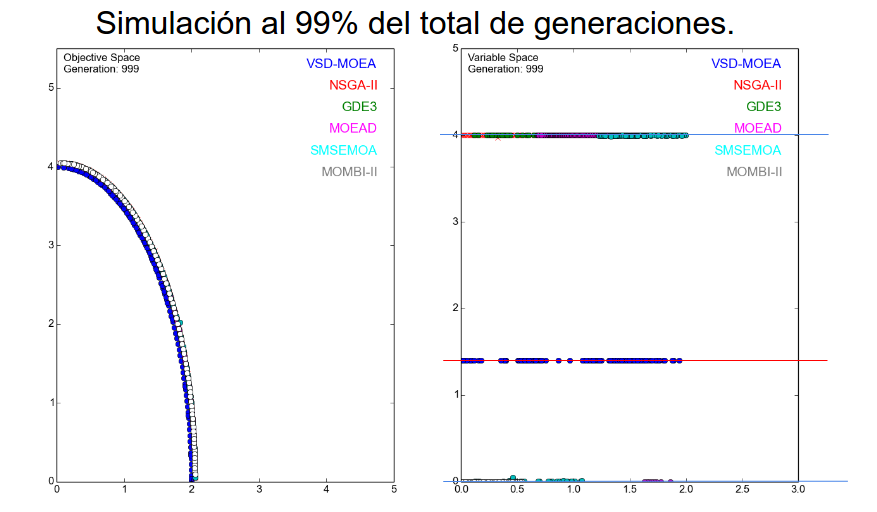
\includegraphics[scale=0.35]
{Figures_Chapter3/Simulacion_Algoritmo_5.png}
\decoRule
\caption{Simulación de la fase de remplazo, al asignar un valor elevado al radio de la hiperesfera.}
\label{fig:Simulacion_Algoritmo_6}
\end{figure}

\section{Complejidad}

La propuesta algorítmica que se describe posee un orden de complejidad elevado, aunque es posible disminuir este orden por medio de procedimientos más sofisticados, se aclara que este trabajo está principalmente orientado en demostrar el efecto que tiene la diversidad en el proceso evolutivo.
%
Sin embargo, se hace una análisis de las secciones cuyo orden de complejidad es más significativo.
%
En esta notación se define a $N$ como el tamaño de la población, $M$ el número de objetivos y $d$ el número de variables.
%En esta notación se define $R$ como el número de individuos de referencia, $C$ el número de individuos candidatos, $M$ el número de objetivos, $P$ el número de individuos penalizados y $d$ el número de variables de decisión.
%

Inicialmante como se indica en el algoritmo \ref{alg:Fase_Remplazo_Complejidad} para identificar a los individuos extremos es necesario realizar $2N$ iteraciones para encontrar a los $M$ mejores individuos de cada función objetivo.
%
Posteriormente, en el ciclo principal el cual es realizado $N-M$ veces (líneas \ref{alg:Calculo_Diversidad_Primero} - \ref{alg:Fase_Remplazo:seleccionarobj}), donde los tres bloques más importantes corresponden a los dos procedimientos para calcular la contribución de diversidad en cada espacio y el método de Ordenación-eficiente-basado-no-dominados.
%
Así, para calcular la contribución de cada individuo en el espacio de las variables (líneas \ref{alg:Calculo_Diversidad_Primero} y \ref{alg:Calculo_Diversidad_Primero_Move}) se realizan $\sum_{i=1}^{N-M}( \sum_{j=1}^{i} ( \sum_{k=1}^{2N-i-M} d ) )$ iteraciones, donde la sumatoria interna corresponde a los individuos candidatos $R_{t}$ los cuales van decrementandose uno a uno en cada iteración, la segunda sumatoria es de los individuos seleccionados los cuales incrementan uno a uno en cada iteración, por último la sumatoria externa indica que en total se realizarán $N-M$ iteraciones, resolviendo la sumatoria se obtiene lo siguiente\footnote{Los cálculos se comprobaron con la herramienta de \href{http://m.wolframalpha.com/input/?i=sum\%5B+sum\%5B+++sum\%5B+d\%2C+k\%2C1\%2C2N-i-M+\%5D+\%2C+\%7Bj\%2C1\%2Ci\%7D\%5D++\%2C+\%7Bi\%2C1\%2CN-M\%7D\%5D}{\textcolor{blue}{Wolfram}}.}:
\begin{equation} \label{eq:costo_contriucion_diversidad}
\begin{split}
\sum_{i=1}^{N-M} \sum_{j=1}^{i} \sum_{k=1}^{2N-i-M}  d = &\\
& -\frac{dM^3}{6} + d M^2 N - \frac{3}{2} d M N^2 - \frac{dMN}{2} + \frac{dM}{6} + \frac{2dN^3}{3} + \frac{dN^2}{2} - \frac{dN}{6}
\end{split}
\end{equation}

Así, para estimar la cota superior sólo se toman los términos dominantes $O(dM^2N + dN^3)$, además se puede observar que el número de variables afecta de forma significativa en la complejidad.
%
En el caso de que estén todos los individuos penalizados y por lo tanto no existan candidatos (líneas \ref{alg:Fase_Remplazo:Vacio} - \ref{alg:Distante_Variables}), se realiza el cálculo de la contribución de diversidad entre los individuos penalizados y los de referencia con el objetivo de seleccionar al individuo con mayor contribución, el peor caso de esta parte es que la diversidad requerida inicialmente se muy elevada y por lo tanto siempre existan individuos penalizados, la complejidad de esta sección es la misma que la indicada en la ecuación \ref{eq:costo_contriucion_diversidad} ya que se realiza el mismo procedimiento, que en lugar de $R_t$ se consideran los individuos \textit{penalizados}, entonces la cota superior es $O(dM^2N + dN^3)$.

%
Por otra parte, para realizar el cálculo de la contribución de cada individuo en el espacio objetivo (línea \ref{alg:Diversidad_Espacio_Objetivo}) y considerando el peor caso que es cuando todos los individuos pertenecen al mismo rango y no existen individuos penalizados, se observa que al aumentar el número de individuos seleccionados decrementa el número de candidatos y además este proceso se realiza $N-M$ veces, por lo tanto se estima que el número de iteraciones por generación es de $\sum_{i=1}^{N-M}( \sum_{j=1}^{i} ( \sum_{k=1}^{2N-i-M} M ) )$, donde la primer sumatoria indica el número de individuos a seleccionar, la segunda corresponde al número de indiviudos seleccionados existentes por iteración y la tercer sumatoria define el número de individuos candidatos.
%
El resultado de esta sumatoria es similar que la ecuación reemplazando $d$ por $M$, donde los términos dominantes son $O(M^3 N + MN^3)$, 

Por último en el procedimiento de \textit{Ordenación-eficiente-basado-no-dominados} se estima que en el peor caso que es cuando no existen individuos penalizados y todos sean del mismo rango la complejidad es de $(N-M)M(2N)^2$.
%

Uniendo cada sección se estima que la complejidad de la fase de reemplazo es:
\begin{equation}
\begin{split}
T(N,M,d) =& c_1 + c_2 + c_3 2N + c_4 + c_5 2N + c_6(N-M) + (c_7+c_9)(dM^2N + dN^3) + c_8(N-M)\\
	 &+ c_{10}(N-M) + c_{11} M(N-M)(2N)^2 + c_{12}(M^3N + MN^3) + c_{13}(N-M) \\
	=& (c_1 + c_2 + c_4) + 2N(c_3 + c_5) + (N-M)(c_6 + c_8 + c_{10} + c_{13}) \\
	&+ (4MN^3 - 4M^2N^2 )c_{11} + (c_7+c_9)(dM^2N + dN^3) + c_{12}(M^3N + MN^3)
\end{split}
\end{equation}
%
Considerando los terminos dominantes se establece que la complejidad del VSD-MOEA es $O(MN^3 + dN^3)$, también se observa que al resolver las sumatorias existen términos negativos, estos indican una cota superior más exacta, aunque para el propósito de esta estimación y por simplicidad son ignorados.
%
El principal motivo de esta estimación, es identificar las secciones con mayor complejidad, se observa que estas secciones corresponden al cálculo de la diversidad en los espacios y a el procedimiento de clasificación por rangos.
%
Entonces, si se requiere bajar el grado de complejidad de este algoritmo se sugiere implementar un método para estimar la diversidad más efectivo y además utilizar una versión más efeciente para el clasificar los rangos de los individuos.
%

En la tabla \ref{tab:Complejidad_Algoritmos} se presentan las complejidades de los algoritmos en el estado-del-arte y el VSD-MOEA, donde el MOEA/D es que tiene un grado de menor complejidad $O(MNT)$ donde $T$ es el tamaño de cada vecindad y los algoritmos de mayor complejidad son el VSD-MOEA y al SMS-EMOA, sin embargo el SMS-EMOA aumenta exponencialmente conforme aumenta el número de objetivos.

\begin{algorithm}[H]
\algsetup{linenosize=\tiny}
  \scriptsize
	\caption{Fase de remplazo del VSD-MOEA} 
	\begin{algorithmic}[1]
    	\STATE Entrada: $P_t$ (Población de la generación actual), $Q_t$ ( Población hijo de la generación actual)
    	\STATE Salida: $P_{t+1}$ \algcost{\textit{Costo}}{\textit{Iteraciones}}
	\STATE $D = D_I - D_I *2* \frac{G_{Transcurridas}}{G_{Final}}$ 	\algcost{$c_{1}$}{$1$}
        \STATE $P_{t+1} = \emptyset$ \algcost{$c_{2}$}{$1$}
        \STATE $R_t = P_t \cup Q_t$ \algcost{$c_{3}$}{$2N$}
         \STATE $Penalizados = \emptyset$ \algcost{$c_{4}$}{$1$}
		\STATE mover( $R_t$,  $P_{t+1}$, Los mejores en cada objetivo) \algcost{$c_{5}$}{$2N$}
        \WHILE{ $|P_t|$ $\leq$ N }  \algcost{$c_{6}$}{\textcolor{gray}{$N-M$}}
			\STATE Calcular \textbf{Diversidad\_Espacio\_Variables} ($R_t$, $P_{t+1}$)  \algcost{$c_{7}$}{$\sum_{i=1}^{\textcolor{gray}{N-M}} \sum_{j=1}^{i} \sum_{k=1}^{2N-i-M}  d $}
		\STATE mover($R_t$, $Penalizados$, Diversidad en el espacio de las variables $ < $ D) \algcost{$c_{8}$}{\textcolor{gray}{$(N-M)$}}
        \IF{$R_t$ está vacío} 
				\STATE Calcular \textbf{Diversidad\_Espacio\_Variables} ($Penalizados$, $P_{t+1}$) \algcost{$c_{9}$}{$\sum_{i=1}^{\textcolor{gray}{N-M}} \sum_{j=1}^{i} \sum_{k=1}^{2N-i-M}  d $}
				\STATE mover($Penalizados$, $R_t$, Más alejado en el espacio de las variables)  \algcost{$c_{10}$}{\textcolor{gray}{$(N-M)$}}
        \ENDIF
		\STATE $ordenaci \acute{o} n-eficiente-basado-no-dominados(R_t \cup P_{t+1}) $  \algcost{$c_{11}$}{\textcolor{gray}{$(N-M)$}$M(2N)^2$}
		\STATE Calcular \textbf{Diversidad\_Espacio\_Objetivo}($R_t$, $P_{t+1})$) \algcost{$c_{12}$}{$\sum_{i=1}^{\textcolor{gray}{N-M}} \sum_{j=1}^{i} \sum_{k=1}^{2N-i-M}  M $}
        \STATE mover($R_t$, $P_{t+1}$, Menor rango en caso de \par
	 \hskip\algorithmicindent empate seleccionar al más alejado en el espacio objetivo)  \algcost{$c_{13}$}{\textcolor{gray}{$N-M$}}
        \ENDWHILE
%	\RETURN $P_{t+1}$
	\end{algorithmic}
    \label{alg:Fase_Remplazo_Complejidad}
\end{algorithm}


% Please add the following required packages to your document preamble:
% \usepackage{graphicx}
\begin{table}[]
\centering
\caption{Complejidad de los MOEAs más populares}
\label{tab:Complejidad_Algoritmos}
\resizebox{\textwidth}{!}{%
\begin{tabular}{|c|c|c|c|c|c|c|}
\hline
\textbf{Algoritmo} & NSGA-II & GDE3 & MOMBI-II & SMS-EMOA & MOEA/D & VSD-MOEA \\ \hline
\textbf{Complejidad} & $O(MN^2)$ & $O(N log^{M-1} N)$ & $O( (N^2) (log(N) + M))$ & $O(MN^2 + N^M)$ & $O(MNT)$ & $O(MN^3 + dN^3 )$ \\ \hline
\end{tabular}%
}
\end{table}

%\section*{Conclusion}

%----------------------------------------------------------------------------------------

% Define some commands to keep the formatting separated from the content 
%\newcommand{\keyword}[1]{\textbf{#1}}
%\newcommand{\tabhead}[1]{\textbf{#1}}
%\newcommand{\code}[1]{\texttt{#1}}
%\newcommand{\file}[1]{\texttt{\bfseries#1}}
%\newcommand{\option}[1]{\texttt{\itshape#1}}

%----------------------------------------------------------------------------------------


\chapter{Algoritmos de Diversidad Basados en Descomposición} % Main chapter title

\label{Chapter4}

\section*{Introducción}


A pesar de que un algoritmo evolutivo tiene la capacidad de proporcionar soluciones próximas a las regiones óptimas en diferentes problemas, existen dificultades de diversos escenarios donde la calidad de las soluciones es degradado de forma considerable.
%
Particularmente, en el caso multi-objetivo es deseable obtener el conjunto óptimo de Pareto, pero en su lugar se han obtenido soluciones aproximadas al frente de Pareto.
%
Algunos métodos clásicos de optimización multi-objetivo se basan en la transformación de un problema de optimización multi-objetivo a un problema de optimización mono-objetivo.
%
Esto se realiza contruyendo funciones de agregación y obteniendo una solución del conjunto óptimo de Pareto a la vez.
%
Los enfoques para transformar un problema multi-objetivo en múltiples problemas de tipo mono-objetivo utilizan la agregación de pesos (WS), la distancia de Tchebycheff (TCH) entre otros.
%

El principal inconveniente de los métodos que pertenecen a optimización clásica, es la necesidad de aplicar múltiples veces un método determinístico con la esperanza de encontrar una solución distinta que pertenezca al óptimo en cada solución (\cite{Joel:Kalyanmoy}).
%
Por otra parte, los algoritmos evolutivos multi-objetivo se han vuelto suficientemente populares, debido a que por su naturaleza pueden obtener múltiples soluciones óptimas de Pareto en una simple ejecución.
%
Las tres metas\footnote{En algunas definiciones la cobertura está comprendida implícitamente.} de un algoritmo evolutivo multi-objetivo son:

\begin{itemize}
\item Encontrar un conjunto de soluciones lo más cercanas al frente de Pareto (conocido como convergencia).
\item Encontrar un conjunto de soluciones bien distribuidas (conocido como diversidad).
\item Cubrir enteramente el frente de Pareto (conocido como cobertura).
\end{itemize}


A pesar de que ya se ha implementado la idea de descomposición por medio de metaheurísticas para resolver problemas de optimización multi-objetivo (\cite{ishibuchi1996multi}, \cite{murata2002cellular}, \cite{jin2001adapting}), este proceso se hizo popular con la introducción de MOEAs basados en descomposicón propuesto por \citeauthor{zhang2007moea}.
%
En el marco de referencia original conocido también como ``MOEA/D'', un problema de optimización multi-objetivo es descompuesto en varios subproblemas de optimización escalar, que son formulados por medio de un enfoque de descomposición tal como el de Tchebycheff utilizando vectores de pesos distribuidos uniformemente.
%
En el MOEA/D, todos los subproblemas son resueltos de forma simultánea, en base a un algoritmo evolutivo que involucra una población de soluciones.
%
Los razgos característicos del marco de referencia comprendido por el MOEA/D consisten en que la relación de vecindad es definida a lo largo de los subproblemas que están basados en la distancia entre sus respectivos vectores de pesos, además se implementa el reemplazo de individuos de forma local.
%


Como ya se ha mencionado anteriormente la mayoría de algoritmos multi-objectivo funcionan sin promover explícitamente la diversidad en el espacio de las varables.
%
%Most Multi-objective Evolutionary Algorithms (MOEAs) operate without explicitly promoting the diversity of the variable space. 
%
Sin embargo, en el dominio mono-objetivo se ha demostrado que manejar apropiadamente este tipo de divesidad debería conducir a soluciones de alta calidad.
%Nevertheless, in the single-objective domain it has been shown that properly managing this kind of diversity might lead to higher-quality solutions.
%
Esta pérdida de diversidad implica una degradación importante en el rendimiento del algoritmo.
%This loss implies an important degradation of the performance.

%

Particularmente, en este trabajo se propone una serie de algoritmos multi-objetivo basados en descomposición y con mecanismos para administrar la diversidad:
\begin{itemize}
\item MOEA/D with Enhanced Variable Space Diversity (MOEA/D-EVSD).
\item MOEA/D with Special Elitism Based in Variable Diversity (MOEA/D-SEBV).
\item Variable Space Diversity MOEA/D (VSD-MOEA/D).
\end{itemize} %denominados en base a sunombrado como ``MOEA/D with Enhanced Variable Space Diversity (MOEA/D-EVSD)''.
%

En especial, el MOEA/D-EVSD se induce la pérdida de diversidad de forma gradual, esto se realiza alterando el proceso de selección para realizar el emparejamiento.
%
Además, se divide el periodo total de ejecución en dos fases: la primera de exploración y la segunda de intensificación, con el propósito de ubicar mejores soluciones en las regiones prometedoras encontradas en la primera fase.
%
%%%%%%%%%%%%%%%%%%%%%%%%%%%%%%5


Las propuestas construidas MOEA/D-EVSD, MOEA/D-SEBV y VSD-MOEA/D son consideradas como extensiones del MOEA/D donde se incluye un control implícito o explícito para mejorar la diversidad en el espacio de las variables.
%
La principal novedad de estas variantes es el hecho de preservar la diversidad en el espacio de las variables mientras que la mayoría de los MOEAs del estado del arte se centran únicamente en preservar la diversidad en el espacio objetivo.
%
Esta propuesta considera el criterio de paro con el objetivo de obtener cambio gradual entre exploración e intensificación.
%

El resto de este capítulo está organizado como sigue.
%
Inicialmente se hace un análisis de los mecanismos de emparejamiento y/o reemplazo que específicamente se han desarrollado en los MOEAs, además se dedica una sección donde se mencionan los métodos generadores de pesos más relevantes en la literatura, esto en base a que el rendimiento de un MOEA depende en gran medida de la distribución que poseen los vectores de pesos.
%
Posteriormente, se describe la propuesta inicial donde se utiliza una selección especial de emparejamiento.
%
En base a los resultados se propone un segundo algoritmo MOEA/D-SEBV el cual tiene como principal característica administrar la diversidad de forma explícita y en función al criterio de paro, además en cada generación se almacena un conjunto de individuos relacionados a cada vector de pesos, así seleccionando al individuo que contribuye más a la diversidad y almacenando al que tenga una mejor aptitud.
%
En la última propuesta algorítmica VSD-MOEA/D se propone una fase de reemplazo con el mismo criterio implementado en el VSD-MOEA, donde se considera un mecanismo conocido popularmente como especiación.
%
Finalmente, se estima la complejidad que tiene cada algoritmo, particularmente se propone una mejora al VSD-MOEA/D para decrementar un orden a la complejidad del mismo.
%

\section{Métodos de descomposición}

En esta sección es realizado un análisis en la literatura de los principales mecanismos de emparejamiento y/o reemplazo, en base a esto son realizadas las propuesta algorítmicas, donde la primer propuesta que consiste en un emparejamiento especial de padres y las dos restantes aplican un mecanismo especial de reemplazo.

\subsection*{Estudios para mejorar el mecanismo de emparejamiento}

A través de la estrategia de dos fases los autores \cite{jiang2016improved} presentaron un esquema guiado por nichos con el objetivo de asignar un rango en la selección para emparejamiento.
%
En este esquema se realiza un conteo en cada nicho de sus subproblemas vecinos. 
%
Así, si el conteo de nichos de un individuo es mayor que un cierto umbral, significa que el individuo es similar a sus subproblemas vecinos y por lo tanto el emparejamiento de padres debe realizarse con los individuos ubicados fuera del vecindario.
%
El estudio experimental indica que la estrategia basada en emparejamiento guiado por nichos, proporciona buenos resultados en problemas que tienen una geometría desconectada en el frente de Pareto.
%

\subsection*{Estudios para mejorar el mecanismo de remplazo}

En la versión original del MOEA/D, se considera el número de soluciones para ser seleccionadas o remplazadas en relación a un subproblema.
%
En el análisis realizado en el MOEA/D-DE (\cite{li2009multiobjective}), se argumentó que para mantener diversidad en la población, el número de veces que se aplica un remplazo debe ser menor.
%
\citeauthor{wang2014replacement} argumentan que una solución nueva la cual corresponde a un subproblema podría no ser la solución más adecuada para sus subproblemas vecinos. 
%
Por lo tanto estos autores propusieron un esquema de remplazo global para el MOEA/D y nombraron al algoritmo como ``MOEA/D-GR''.
%
En este estudio, se definen dos vecindarios como: el vecindario de emparejamiento y el vecindario de remplazo, los cuales son considerados para cada subproblema, particularmente se analiza el efecto que tiene el tamaño del vecindario de remplazo.
%
En el estudio experimental, concluyeron que al incorporar el esquema GR en el MOEA/D el número de individuos que se deben remplazar por cada vecindario es generalmente distinto para problemas diferentes.


\citeauthor{wang2016adaptive} ampliaron el esquema GR y además desarrollaron un esquema GR adaptativo.
%
Los autores argumentaron que un tamaño pequeño del vecindario para realizar el remplazo es bueno para fomentar la exploración al inicio del proceso de búsqueda, mientras que un tamaño grande es bueno para fomentar la explotación al final del proceso de búsqueda.
%
En este estudio son investigados tres esquemas adaptativos distintos para ajustar el tamaño de la vecindad de remplazo, los cuales se basan en funciones lineales, exponenciales y de sigmoid, además indican que la función de sigmoid basada en un esquema adaptativo proporciona los mejores resultados.
%
Basados en la estrategia adaptativa de remplazo se presentan los algoritmos MOEA/D-AGR y MOEA/D-GR en varios problemas de pruebas.
%
Los resultados experimentales demostraron que los algoritmos basados en el esquema GR mejoran a los algoritmos del estado-del-arte.
%
Entre los algoritmos basados en el esquema GR, el MOEA/D-AGR es el que proporciona mejores resultados a través de todos los problemas de prueba.


Los autores \citeauthor{li2014stable} sugirieron incorporar un modelo de concordancia estable (STM) para coordinar la selección de soluciones prometedoras para los subproblemas en el MOEA/D.
%
En el algoritmo nombrado MOEA/D-STM, se realiza la clasificación de todas las soluciones que corresponden al conjunto de soluciones (ejemplo soluciones padres e hijos), utilizando sus respectivos valores en la función de agregación, y se proporciona una preferencia a las soluciones con mejores valores en sus funciones de agregación, fomentando la convergencia.
%
De lo contrario, cada solución clasifica por medio de rangos a todos los subproblemas de acuerdo a la distancia de los vectores direccionales que corresponden a los subproblemas, y se expresa la preferencia para los subproblemas con una distancia menor, entonces así es promovida la diversidad.
%
El modelo STM enlaza cada subproblema a sólo una solución de tal forma que se mantiene el balance entre convergencia y diversidad.
%
Los estudios experimentales demostraron que el MOEA/D-STM es significativamente superior a varios MOEAs del estado-del-arte en las instancias de prueba UF (\cite{zhang2008multiobjective}).


\citeauthor{li2015interrelationship} presentaron una extensión del MOEA/D-STM y el MOEA/D-IR (\cite{li2014stable}), el primero se basa en la interrelación se los subproblemas para realizar la selección del MOEA/D, mientras que el segundo define preferencias mutuas entre los subproblemas y la soluciones.
%
Sin embargo, el MOEA/D-IR define una relación de preferencia entre un subproblema y una determinada solución.
%
El estudio experimental demostró que el MOEA/D-IR es significativamente superior en varios problemas de prueba que algunos MOEAs del estado-del-arte incluyendo al MOEA/D-STM.

Posteriormente, \cite{gee2015online} presentaron una métrica de diversidad  \textit{online} obtenida por un MOEA.
%
Los autores introdujeron una medición de la diversidad, nombrada como Pérdida Máxima de la Diversidad Relativa (\textit{Maximum Relative Diversity Loss} - MRDL), para estimar la pérdida de diversidad de una solución para toda la población.
%
En orden para validar la métrica propuesta, los autores incorporaron la métrica en el marco de referencia del MOEA/D.
%
Específicamente se introduce un operador de selección nuevo en el MOEA/D, donde cada solución hijo es revisado para su MRDL, y posteriormente se realiza el proceso de remplazo.
%
Si el RMDL que corresponde a una solución hijo es mayor que un determinado umbral, se selecciona en su lugar a la solución padre, de forma que la diversidad es mantenida.


\subsection*{Estudios para mejorar el mecanismo de emparejamiento y remplazo}

Además de la introducción de los operadores de evolución diferencial en el MOEA/D, (\cite{li2009multiobjective}) refinaron al marco de referencia del MOEA/D agregando dos parámetros.
%
La primera medición permite que las soluciones padres sean seleccionadas durante la reproducción con una baja probabilidad para toda la población (por ejemplo afuera del vecindario).
%
La segunda aportación agrega un límite superior en el número máximo de soluciones que se pueden reemplazar por una solución hijo durante la actualización de cada vecindario.
%
La introducción de estos mecanismos fomentan la la diversidad en la población.


Por otra parte, los autores \cite{ishibuchi2009effects} consideraron al MOEA/D como un algoritmo celular donde cada celda tiene su propia función de escalarización de aptitud con cada vector de pesos.
%
En los algoritmos evolutivos celulares estándares, una solución hijo es únicamente comparada con la solución reciente en su celda.
%
En este estudio los autores investigaron el efecto del remplazo local en el MOEA/D celular.
%
En particular, los autores examinaron el impacto de adoptar distintas estructuras de vecindarios para la selección y remplazo.
%
El estudio experimental demostró que el remplazo en el vecindario local, tiene un rol clave en el rendimiento del MOEA/D.
%

Para resolver el problema de selecionar un adecuado tamaño de la vecindad para distintos problemas, \cite{zhao2012decomposition} propusieron el algoritmo ENS-MOEA/D.
%
En este algoritmo son utilizados distintos tamaños de vecindarios donde las probabilidades de selección se ajustan dinámicamente en base a su rendimiento histórico de generar soluciones prometedoras.
%
El estudio experimental demostró la superioridad del ENS-MOEA/D contra el MOEA/D-DRA con tamaños de vecindades fijos en los problemas de prueba UF.
%


\cite{giagkiozis2014generalized} presentaron un algoritmo nombrado MACE-gD.
%
Cuya principal característica es que el control de la estructura en los vecindarios es por medio de un parámetro.
%
Este parámetro indica el porcentaje de soluciones superiores en la población nueva con respecto a un subproblema, los cuales son utilizados para construir un modelo de probabilidad por medio del método CE.
%
Entonces, la relaciones entre los vecindarios son dinámicamente actualizados con respecto al espacio objetivo.
%
Además en la fase de remplazo, sólo se compara una nueva solución del subproblema con su respectiva solución actual.


Posteriormente, \cite{zhang2016self} propusieron una variante del MOEA/D, denominada SMOEA/D, basado en un mecanismo de reproducción auto-organizado (Self-organizing Reproduction Mechanism-SRM).
%
En el SRM, en cada generación se aplica un mapeo de auto-organización, esto para determinar la estructura de distribución de la población (en el espacio de las variables) y construir un conjunto de emparejamiento para cada solución.
%
Además, otra característica del SRM es que implementa un ajuste adaptativo en la probabilidad para seleccionar distintos tamaños de vecindades, este ajuste es basado en el rendimiento de las soluciones generadas a través de un cierto número de generaciones previas.
%
La estrategia de remplazo del SMOEA/D es basado en una estrategia \textit{greedy} o glotona, esta consiste en que dada una nueva solución se actualizan los dos subproblemas en los cuales se muestra una máxima mejora en términos de la función de aptitud agregada.
%
El estudio experimental realizado en distintos subproblemas de prueba con geometrías de Pareto y conjuntos de Pareto complicados, revelan que el SMOEA/D es superior al MOEA/D-DE (\cite{li2009multiobjective}) y al RM-MEDA en cada problema de prueba.
%
La limitación del SMOEA/D es su mayor complejidad computacional y además induce cuatro parámetros adicionales.



\section{Métodos generadores para los vectores de pesos}

Los algoritmos basados en descomposición requieren de un conjunto de vectores de pesos para convertir un problema multi-objetivo en un conjunto de problemas mono-objetivo.
%

La versión original del MOEA/D (\cite{Joel:MOEAD}) y otras variantes implementan el enfoque de \cite{das1998normal}, conocido como método de diseño \textit{símplex-lattice} el cual genera vectores de pesos distribuidos uniformemente en el simplex, sin embargo en este método el tamaño de la población crece dramáticamente conforme el número de objetivos aumentan y por lo tanto el tamaño de la población no es flexible.
%
Además, para el caso de tres o más objetivos la distribución de los vectores de pesos no es muy uniforme.
%


Principalmente este método consiste en generar vectores de pesos igualmente espaciados.
\begin{equation}
\Lambda = \left  \{  \vec{\lambda} | \lambda_i \in \left \{ 0, \frac{1}{H}, \frac{2}{H},...,\frac{H-1}{H} \right \}, i=1, ..., k, \quad s. a. \quad \sum_{i=1}^{k} \lambda_i = 1 \right \}
\end{equation}
donde $H$ representa el número de divisiones en cada objetivo.


%
Este método generador de pesos tiene tres inconvenientes (\cite{finkenstadt2006statistical, berengueroptimizacion}):
\begin{itemize}
   \item La distribución de los vectores de pesos no es  muy uniforme al considerar muchos objetivos.
   \item Para distribuir los vectores de pesos, el número de vectores generados aumenta de forma lineal conforme aumenta el número de objetivos, esto indica que para $m$ objetivos el número de vectores de pesos necesarios es $\binom{H+m-1}{m-1}$.
   \item La mayor parte de los vectores están distribuidos en la frontera del símplex.
\end{itemize}


\cite{Joel:MOEAD_AWA} propusieron un método para inicializar a los vectores de pesos, conocida como \textit{transformación WS}, basado en la relación geométrica entre los vectores de pesos y la soluciones óptimas correspondientes considerando el enfoque de Tchebycheff.
%
El estudio experimental demuestra que la \textit{transformación WS} en tres objetivos propicia soluciones óptimas bien distribuidas.


Alternativamente, otro método generador de pesos ampliamente utilizado en muchas variantes del MOEA/D se basa en un paradigma de muestreo aleatorio uniforme.
%
Una de las principales ventajas de este último método es que el tamaño de la población es flexible.
%



Similarmente en \cite{tan2012modification}, \cite{tan2013moea}, \cite{ma2014moea}, \cite{berengueroptimizacion} sugieren utilizar el método \textit{glp (good lattice point)} (\cite{fang1994number}) y el diseño uniforme (DU) (\cite{fang1980uniform}) para generar los vectores de pesos.
%
Los autores \citeauthor{berengueroptimizacion} indican que el método \textit{glp} tiene un costo computacional elevado conforme aumenta el número de objetivos en el problema, por lo tanto proponen el método de Harmmersley (\cite{talke2012number}) el cual sirve para obtener un conjunto de puntos uniformemente dispersos en el espacio como alternativa al \textit{glp}.
%
Este último se considera como un método cuasi Monte-Carlo y es definido como un método de baja discrepancia.
%
El método de Hammersley se basa en la representación de los número naturales, donde cualquier entero positivo $k$ se puede expresar de manera única utilizando como base un número primo $p \geq 2$.
\begin{equation}
k = \sum_{i=0}^n b_i  p^i. \quad 0 \leq b_i \leq p-1, \quad i=0,....,n
\end{equation}
%
Sea $k \geq 2$ y $P = \{ p_1, ..., p_{k-1} \}$ un conjunto de $k-1$ primos, formalmente se denomina como el \textit{conjunto de Hammersley} a los $n$ puntos uniformemente dispersos en el espacio $[0, 1]^k$ donde:
%
\begin{equation}
   x_i = \left [ \frac{2i-1}{2n}, y_{p1(i)}, ..., y_{pk-1}(i)  \right ]^T, \quad i=1, ..., n.
\end{equation}
%

%
La discrepancia es considerada como una medida de uniformidad (\cite{talke2012number}).
%
Particularmente, la secuencia de Harmmersley tiene un orden de $O((log (n) )^m / n)$, donde $n$ es el número de puntos y $m$ es el número de objetivos.


\citeauthor{yuan11number} propusieron un método de transformación para obtener el conjunto de vectores de pesos $\Lambda$ que estén dispersos uniformemente en el símplex, donde cada vector de pesos $\lambda$ debe cumplir la restricción $\sum_{i=1}^{m-1} \lambda_i = 1$.
%
Específicamente, dado un conjunto de puntos $U = \{u_1, u_2, ..., u_n \}$ de baja discrepancia en el dominio $[0, 1]^{m-1}$ se puede realizar la transformación de estos puntos en los vectores de pesos  $\Lambda = \{ \lambda_1, \lambda_2, ..., \lambda_n \}$ de la siguiente manera:
%
\begin{equation}\label{Transformacion_Uniformes}
\begin{split}
\lambda_{i}^k &= ( 1 -  u_{k,i}^{\frac{1}{m-i}} ) \prod_{j=1}^{i-1} u_{k,j}^{\frac{1}{m-j}} \quad i=1,..., m-1\\
\lambda_{i}^m &= \prod_{j=1}^{m-1} u_{k,j}^{\frac{1}{m-j}}
\end{split}
\end{equation}

El método generador utilizado en este trabajo consite en el método previamente mencionado, es decir, se generan los puntos por medio del método de Hamersley y posteriormente se transforman a un conjunto de vectores de pesos, como es mencionado en \cite{berengueroptimizacion}, el algoritmo \ref{alg:Generador_Pesos} muestra los pasos a seguir para este procedimiento.
%

%
 \begin{algorithm}[!t]
\caption{Generador de los vectores de pesos por medio del método de Hammersley}
\label{alg:Generador_Pesos}
%\begin{scriptsize}
\begin{algorithmic}[1]
    \STATE Entrada: número de objetivos ($m$), número de los vectores de pesos ($|\Lambda|$).
    \STATE Salida: Conjunto de vectores de pesos $\Lambda$.
    \STATE $p$= los primeros $k-2$ números primos.
    \STATE $U$= $\emptyset$.
    \FOR{$i=1$ hasta $n$}
        \STATE $u_{i,1} = (2i - 1)/2n$
	\FOR{$j=2$ hasta $k-1$}
	   \STATE $u_{i,j} = 0$
	   \STATE $f = 1/p_{j-1}$
	   \STATE $d = i$
	   \WHILE{$d>0$}
		\STATE $u_{i,j} + f  ( d \quad mod \quad p_{j-1})$
		\STATE $d = \lfloor d / p_{j-1} \rfloor$
		\STATE $f =  f/p_{j-1}$
	   \ENDWHILE
	\ENDFOR
	\STATE $U = U \cup u$
    \ENDFOR
    \STATE $\Lambda = $ implementar la tranformación (\ref{Transformacion_Uniformes}) a cada elemento de $U$.
\end{algorithmic}
%\end{scriptsize}
\end{algorithm}


En la figura \ref{fig:simplex_puntos} se muestra la distribución de los puntos en el simplex, se puede observar que el método de simplex-lattice genera más puntos en la frontera conforme incrementa el número de objetivos en comparación al método de diseño uniforme. 

\begin{figure}[H]
\centering
\scriptsize
%\includegraphics[width=6cm, height=6cm]
\includegraphics[scale=0.27, angle=-90,origin=c]
{Figures_Chapter4/simplex.eps}
\includegraphics[scale=0.27, angle=-90,origin=c]
{Figures_Chapter4/uniform.eps}
\decoRule
\caption{Puntos distribuidos en el simplex, en la parte izquierda se muestran los puntos generados por el diseño simplex-lattice y en la derecha por diseño uniforme, en cada uno se consideran 105 puntos.}
\label{fig:simplex_puntos}
\end{figure}



Los autores \cite{Joel:MOEAD_AWA} argumentaron que los vectores de pesos distribuidos uniformemente en el MOEA/D no puede asegurar una distribución uniforme cuando la geometría del frente de Pareto es compleja (por ejemplo en forma discontinua, picos agudos o colas bajas).
%
Por lo tanto propusieron una estrategia para adaptar a los vectores de pesos (AWA), resultando en el algoritmo MOEA/D-AWA, el cual es basado en una estrategia de dos etapas, donde primero se utiliza un conjunto de vectores de pesos predeterminados hasta que el algoritmo converge a un cierto grado.
%
Posteriormente, los vectores de pesos son ajustados de tal forma que algunos subproblemas son eliminados de las partes más pobladas o con muchos puntos en el frente de Pareto y algunos subproblemas son agregados en las partes con mayor diversidad o en regiones discontinuas del frente de Pareto.
%
Además, el MOEA/D-AWA implementa una población externa para almacenar las soluciones no dominadas y para guiar al algoritmo en la eliminación y adición de subproblemas.
%
El estudio experimental indica que el MOEA/D-AWA mejora al estado del arte con problemas cuyo frente de Pareto está comprendido por una geometría irregular.
%


Posteriormente, \cite{jiang2016towards} presentaron una variante del MOEA/D con un archivo basado en el hipervolumen rápido, nombrado como FV-MOEA/D. 
%
En este algoritmo, se almacenan las soluciones no dominadas, por lo tanto las soluciones candidatas son agregadas o descartadas de tal forma que el archivo que corresponde al hipervolumen es maximizado.
%
La principal idea del FV-MOEA/D es que periódicamente se adaptan los vectores de pesos basados en las soluciones del archivo externo.
%
Los estudio experimentales demostraron la eficiencia del MOEA/D con distintos problemas de optimización multi-objetivo con diferentes geometrías de Pareto.

Por otra parte los autores \citeauthor{giagkiozis2013towards} en el \citeyear{giagkiozis2013towards} argumentaron que la adaptación de pesos en un algoritmo basado en descomposición puede generar una nueva dificultad en el proceso de búsqueda.
%
Esto se debe porque cuando los vectores de pesos son fijados, los subproblemas a resolverse también permanecen fijos.
%
Sin embargo, cuando los vectores de pesos son adaptados, también cambian los subproblemas asociados.
%
Entonces, los autores recomendaron las estrategias para adaptar a los vectores de pesos deben ser cuidadosamente investigados antes de su implementación.
%

Recientemente los autores \cite{li2015evolutionary} propusieron un método generador, el cual se basa en el método de \citeauthor{das1998normal}, este  método realiza la clasificación de dos tipos de vectores: ubicados en la frontera del símplex y ubicados en el interior del símplex, para realizar este proceso se consideran dos configuraciones, así los vectores que pertenecen al interior del simplex se obtienen contrayendo los vectores generados mediante otra configuración, entonces el conjunto de vectores finales es la unión de los dos conjuntos.


\section{Enfoques para convertir un problema multi-objetivo a mono-objetivo}

En el capítulo \ref{Chapter2} se presentaron tres métodos para la descomposición de un problema multi-objetivo en varios problemas mono-objetivo, aunque el enfoque de Tchebycheff es uno de los más implementados, en su lugar se ha propuesto el enfoque de función de escalarización (ASF), este último que describe las direcciones óptimas de acuerdo a los vectores de pesos en el espacio objetivo, en consecuencia provee una mayor escalabilidad al problema.
%
En la práctica se ha observado que tanto en el enfoque de Tchebycheff como en el ASF existe una desventaja importante.
%
Cada función de aptitud es únicamente asociada a un subproblema mediante un objetivo, por lo tanto los vectores de pesos que están ubicados en las esquinas del símplex no consideran a las funciones objetivo restantes, además las soluciones son óptimo de Pareto débiles \citep{miettinen2002scalarizing}.

Por lo tanto, si se desea evitar a las soluciones que son óptimo de Pareto débiles, se puede utilizar su forma aumentada, que en el caso de Tchebycheff es definido de la forma \citep{ishibuchi2010simultaneous, derbel2014impact}:
\begin{equation}
\label{eqn:Tch_augmented}
\begin{split}
minimizar \quad g^{AT}( \vec{x} | \vec{\lambda}, \vec{z^*} ) = \max\limits_{i \in {1,...,m}} \left \{ \lambda_i | f_i(x) - z^*_i|   \right \} + \rho \sum_{j=1}^m |f_i(x) - z_j^*|,
\end{split}
\end{equation}
donde $\rho$ usualmente es una constante muy pequeña (ejemplo $0.1$).
%
De esta forma se considera la calidad de los demás objetivos, y su relevancia es configurada con el parámetro $\rho$.
%

Por otra parte, debido a que la función ASF tiene un mejor desempeño, en este trabajo se propone la función de escalarización aumentada (ASFA), definida de la forma:
\begin{equation}
\label{eqn:ASF_augmented}
\begin{split}
minimizar \quad g^{asfa}( \vec{x} | \vec{\lambda}, \vec{z^*} ) = \max\limits_{i \in {1,...,m}} \left \{  \frac{ | f_i(x) - z^*_i|}{\lambda_i}   \right \} + \rho \sum_{j=1}^m |f_i(x) - z_j^*|,
\end{split}
\end{equation}

La función de escalarización aumentada, considera el desempeño del peor objetivo y parcialmente de los demás objetivos, por lo tanto los resultados serán de mejor calidad, y se podrán obtener funciones óptimas de Pareto fuertes.

%%%Aportaciones...........................................
\section{Propuesta con selección especial de padres (MOEA/D-EVSD)}


La propuesta inicial MOEA/D-EVSD extiende el tradicional MOEA/D.
%
Particularmente, el MOEA/D-EVSD es un MOEA basado en descomposición que implementa cualquier enfoque\footnote{En capítulo 2 se definen los enfoques más utilizados en el ámbito multi-objetivo.} para generar un conjunto de subproblemas de optimización mono-objetivo.
%
El MOEA/D-EVSD está dividido en dos fases: la primera fase inicia con un grado de exploración elevado, y ésta va cambiando gradualmente hacia la explotación, por lo tanto la segunda fase es dedicada totalmente a la intensifacación.
%
La principal característica de la primera fase es que se implementa un enfoque de emparejamiento especial como parte del proceso de selección (revisar algoritmo ~\ref{alg:MOEAD_EVSD}).
%
Similarmente al MOEA/D,  cada subproblema tiene un vecidario donde su tamaño es denotado por $T_r$.
%
El propósito de alterar la selección de padres es tener un mejor control de la diversidad que se induce en el espacio de las variables.
%
Similarmente al MOEA/D, para cada subproblema $P_i$, se crea un nuevo individuo.
%
Es bien sabido que en la mayoría de operadores de cruce, tal como en el SBX, el poder de exploración incrementa cuando se toman en cuenta individuos distantes.
%
Entonces, un enfoque heurístico para tratar de inducir diversidad consiste en promover el emparejamiento de individuos diferentes.
%
Así, en nuestra propuesta es modificado el proceso de selección en el emparejamiento del MOEA/D. 
%
Especialmente, en lugar de seleccionar aleatoriamente a dos individuos del vecindario de $B_i$ para continuar con el proceso de emparejamiento, se implementan los siguientes pasos.
%
Primero, se llena un conjunto $P$ de padres candidatos con tamaño $\alpha$.
%
Cada candidato padre es seleccionado aleatoriamente del vecindario en el problema $P_i$ con una probabilidad $\delta$, mientras que la probabilidad de seleccionar padres de la población entera es de $1-\delta$.
%
Posteriormente, son seleccionados los dos individuos cuya distancia sea la mayor en el proceso de emparejamiento.
%
El proceso anterior requiere fijar el parámetro $\delta$ para llenar el conjunto de emparejamiento.
%
Desde que se busca alterar el grado de exploración dinámicamente, este parámetro es asignado de la siguiente forma: $\delta = \frac{t_i}{Total\quad Generaciones}$, donde $t_i$ denota la generación actual.
%
De esta forma, al principio de la primera fase, cada individuo es seleccionado considerando a la población entera, pero esta proporción de individuos seleccionados globalmente es linealmente decrementado durante la ejecución.
%
Así, es inducido un cambio gradual entre exploración y explotación.
%

En el algoritmo \ref{alg:MOEAD_EVSD} se muestra el proceso de emparejamiento que corresponden a la primera fase, este es incorporado con el esquema del MOEA/D.
%
Las líneas \ref{alg:Inicializar_Vectores_Pesos}-\ref{alg:Inicializar_Referencia} consisten en generar los vectores de pesos mediante algún método en específico, la inicialización de la población y del vector de referencia.
%
Este último es utilizado en el enfoque para convertir el problema a múltiples problemas mono-objetivo, usualmente se considera tanto el vector nadir como el ideal ($z^{nan}$, $z^*$).
%
Posteriormente en cada generación se realizan los pasos como se indica a continuación.
%
Se selecciona un conjunto para el emparejamiento, se implementa a la reproducción dados dos individuos seleccionados del conjunto de emparejamiento, es actualizado el vector de referencia y se actualizan las soluciones vecinas (líneas \ref{alg:Emparejamiento} - \ref{alg:Actualizar_Vecindarios}).
%
En este esquema se consideran dos fases, la primera es dedicada a la exploración, y la segunda a la intensificación.
%
Particuarmente, en la segunda fase se implementa un procedimiento de mejora donde se pueda ofrecer un grado significativo de intensificación, en el caso mono-objetivo se utiliza popularmente una búsqueda local como es indicado en la línea \ref{alg:Busqueda_Local}.
%
Posteriormente en la segunda fase se implementa un proceso de búsqueda diferente por medio de los operadores de evolución diferencial, también se hace mención de la importancia que reside en asignar adecuadamente el parámetro $T_r$.
%
El parámetro $T_r$ de la primera y segunda fase son identificados respectivamente por $T_{r,1}$ y $T_{r,2}$, además el efecto de este parámetro en la primera fase es de exploración ya que es considerado un tamaño de vecindad pequeño, en el caso contrario es de intensificación explicado por \citeauthor{Joel:MOEAD_Adaptative} en su trabajo \cite{Joel:MOEAD_Adaptative}.

\begin{algorithm}[!t]
\caption{MOEA/D-EVSD}\label{alg:MOEAD_EVSD}
\begin{scriptsize}
\begin{algorithmic}[1]
    \STATE Inicializar los vectores de pesos $\lambda^1, \lambda^2, ..., \lambda^N$ y vecindarios $B(i)$ utilizando el enfoque tradicional del MOEA/D. \label{alg:Inicializar_Vectores_Pesos}
    \STATE Generar una población inicial de forma aleatoria $x^1, ..., x^N$.
    \STATE Inicializar $z = (z_1, ..., z_m)^T$ con un valor elevado. \label{alg:Inicializar_Referencia}
  \WHILE {(no se cumpla el criterio de paro)}
  \FOR{i=1,...,N}
    \STATE \textbf{Conjunto para emparejamiento}: Llenar aleatoriamente el conjunto de emparejamiento $P$ con los individuos $\alpha$, seleccionando cada individuo del vecindario $B(i)$ con probabilidad $\delta$ o de la población complta con probabilidad $(1 - \delta)$. \label{alg:Emparejamiento}
    \STATE \textbf{Reproducción}: Seleccionar a los individuos más distantes de $P$ e implementar los operadores genéticos para generar nuevos individuos (y).
    \IF{ Segunda fase}
	\STATE \textbf{Búsqueda Local}: Implementar cruza y mutación de evolución diferencial en el vecindario $B(i)$. \label{alg:Busqueda_Local}
    \ENDIF
    \STATE \textbf{Actualizar el vector de referencia $z$}: Para cada j = 1,..,m, if $z_j > f_j(y)$, entonces asignar $z_j = f_j(y)$.
    \STATE \textbf{Actualizar las soluciones vecinas}: Para cada índice $j \in B(i)$, si $g(y| \lambda^j, z) < g(x_j| \lambda^j, z)$, entonces asignar $x^j = y$.\label{alg:Actualizar_Vecindarios}
    \ENDFOR
       \STATE Actualizar el valor $\delta$
  \ENDWHILE
\end{algorithmic}
\end{scriptsize}
\end{algorithm}


\subsection{Fase de intensificación}

Particularmente, en esta fase se aplican los operadores de evolución diferencial, el efecto de estos operadores en el proceso de búsqueda depende en la distribución de los individuos en el espacio factible ya que este proceso puede ser de intensificación o exploración de acuerdo a la ubicación de los individuos.
%
Específicamente , es aplicado el esquema o estrategia \textit{Rand/1/bin} para generar nuevos individuos, donde \textit{Rand} indica que los vectores base son escogidos de forma aleatoria, \textit{1} significa que únicamente se utiliza un vector de diferencia para formar a la población mutada, y el término \textit{bin} (de distribución binomial) indica que se implementa la cruza uniforme durante la formación de una población (\cite{Storn1997}).
%
El proceso para generar un nuevo individuo $x^{new}$ consiste en seleccionar tres individuos distintos $x_1$, $x_2$ y $x_3$ (como se indica en la ecuación \ref{eq:DE_Operator}), el parámetro de cruza $CR$ controla la invarianza rotacional en el proceso de búsqueda y el factor de mutación $F$ controla la velocidad de convergencia y robustez en la búsqueda (\cite{kukkonen2009performance}).
%
\begin{equation} \label{eq:DE_Operator}
x =
  \begin{cases}
    x_{1,i} + F*(x_{2,i} - x_{3,i}  ) &: \text{ rand $< CR$ OR $i == I_{rand}$} \\
    x_{1,i} &: \text{de otra forma} 
  \end{cases}
\end{equation}%


Alternativamente, en esta fase se puede implementar la búsqueda local SQA indicada por \citeauthor{Joel:LOCALSEARCH}, que consiste en una proximación cuadrática simplificada.
%
El método SQA es una busqueda directa y es puramente heurística.
%
Dados tres puntos cuyo valor objetivo es mínimo $x^a$, $x^b$ y $x^c$, se genera un punto aproximado cuyo valor mínimo $x^i$ es calculado de la forma:
\begin{equation}
x_k^i = \frac{1}{2} \frac{A_k}{B_k} \quad k=1,...,n
\end{equation}
donde\\
\begin{equation*}
\begin{split}
A_k &=[(x_k^b)^2 - (x_k^c)^2] f(x^a) + [(x_k^c)^2 - (x_k^a)^2] f(x^b) + [(x_k^a)^2 - (x_k^b)^2] f(x^c) \\
B_k &=(x_k^b - x_k^c) f(x^a) + (x_k^c - x_k^a) f(x^b) + (x_k^a - x_k^b) f(x^c)
\end{split}
\end{equation*}

En contraste a otros optimizadores locales basados en el gradiente, el SQA no necesita el cálculo de gradiente lo cual amplía su implementación en problemas de optimización.
%
A diferencia de otros modelos de aproximación cuadrática no se necesitan varias incógnitas de la función objetivo para construir el modelo cuadrático, el SQA en una aproximación cuadrática basada en tres puntos, y es de fácil implementación.
%
Así, la aproximación cuadrática simplificada hace un buen uso de los valores que corresponden a la función objetivo -- es resuelta en cada iteración para dar un paso a la solución del problema.

\subsection{Observaciones}
Los autores  \cite{Joel:STUDY_MATTING_RESTRICTION} examinan el efecto de implementar restricciones de emparejamiento en MOEAs, donde concluyen que el grado de similitud entre los individuos seleccionados para emparejarse está altamente relacionado con el proceso de exploración, así emparejar individuos similares acelera la velocidad de convergencia y decrementa la diversidad.
%
En el algoritmo propuesto se desea implementar un balance ideal de búsqueda por medio de distintas fases, sin embargo existe un inconveniente importante: hay una tendencia de seleccionar a los individuos que se encuentran principalmente en las esquinas y ligeramente en la frontera del espacio factible, esto se puede intuir ya que las regiones más distantes están ubicadas (dependiendo del espacio factible) en la frontera.
%
Alternativamente, se puede demostrar la tendencia de esta heurística de la siguiente forma. 
%
Se selecciona una muestra dados un conjunto de puntos distribuidos de forma uniforme en el espacio, entonces los puntos más alejados de este conjunto de puntos pertenecen al envolvente convexo, por lo tanto la tendencia consiste en selecccionar a los puntos que pertenecen al envolvente convexo, si se seleccionan muestras parciales del espacio de búsqueda, entonces en promedio se seleccionan a los individuos más distantes que pertenecen al envolvente convexo del espacio factible, que en este caso son las esquinas.
%


Para demostrar esta tendencia, se realizaron dos simulaciones, en cada una se generaron 500 puntos mediante una distribución uniforme en un espacio cuyos límites están comprendidos por $[-1, 1]^2$, en cada simulación se seleccionaron 10 muestras con remplazo de tamaño 4 y 20 respectivamente.
%
En las figura \ref{fig:Simulacion_Mating} se observan los puntos que comprenden el envolvente convexo de cada muestra (puntos de con color azul) y el área que domina cada uno (delimitado por líneas de color rojo), un efecto importante de aumentar el tamaño de las muestras es que cada envolvente convexo está más próximo a los límites del espacio factible, por lo tanto al seleccionar a los dos puntos más alejados de cada muestra tiende a seleccionar las esquinas del espacio factible como se puede observar en la parte derecha de la figura \ref{fig:Simulacion_Mating}.
%

\begin{figure}[H]
\centering
\scriptsize
\includegraphics[scale=0.4]
{Figures_Chapter4/Mating_sample_4_points_500_gen_10.eps}
%%\decoRule
%%\label{fig:Simulacion_Mating_1}
%%\end{figure}
%%
%%\begin{figure}[H]
%%\centering
%%\scriptsize
%\includegraphics[width=6cm, height=6cm]
\includegraphics[scale=0.4]
{Figures_Chapter4/Mating_sample_20_points_500_gen_10.eps}
\decoRule
\caption{Simulación del proceso de emparejamiento, en la parte izquierda el tamaño de cada muestra es de 4 puntos y en la derecha de 20 puntos, se observa la tendencia de seleccionar a los individuos que corresponden al espacio factible.}
\label{fig:Simulacion_Mating}
\end{figure}

Existe la posibilidad de que con esta propuesta surgan inconvenientes de diversidad en algunos problemas de prueba, ya que este proceso de emparejamiento especial únicamente retrasa la convergencia, sin embargo en la situación especial donde las regiones subóptimas estén ubicadas en las esquinas de la región factible se tendrá un efecto de estancamiento en el proceso de búsqueda.

%%
\section{Propuesta de diversidad con elitismo especial (MOEA/D-SEBV)}

En la propuesta inicial se observa que existe una tendencia de seleccionar individuos en las esquinas del espacio de búsqueda, además aún es posible tener un efecto similar a la convergencia prematura, por lo tanto esta segunda propuesta está estructurada con el propósito de mantener la diversidad en el espacio de las variables de forma explícita.
%
En el capítulo 3 se presentó el algoritmo VSD-MOEA donde se aplica una fase de remplazo para mantener la diversidad explícitamente, en este proceso se verifica la contribución de diversidad que tiene cada individuo en el espacio de las variables por medio de la distancia al vecino más cercano, particularmente se prefieren a los individuos cuya distancia al vecino más cercano sea mayor que un umbral.
%
Conforme transcurren las generaciones este umbral es decrementado en base a un modelo lineal.
%
En base a este mismo principio se desea mantener la diversidad en esta segunda propuesta de descomposición.


El marco de referencia que corresponde al MOEA/D establecido por \citeauthor{Joel:MOEAD} fomenta un grado elevado de elitismo ya que constantemente se remplazan los individuos con mayor aptitud de cada vecindario.
%
Aunque en la literatura multi-objetivo se ha establecido que los MOEAs con propiedades elitistas proporcionan mejores resultados (\cite{Joel:Kalyanmoy}), se ha observado que es importante administrar el grado de elitismo, ya que en algunos escenarios (por ejemplo ejecuciones de largo plazo) el proceso de búsqueda puede estancarse.
%
El problema de convergencia prematura se puede observar en la figura \ref{fig:Ubicacion_Lambda} donde son considerados cuatro individuos $\{x_1, x_2, x_3, x_4\}$ y los vectores de pesos $\{ \lambda_1, \lambda_2, \lambda_3 \}$, en el proceso de actualización el individuo $x_4$ será asignado a todos los subproblemas ocasionando problemas de diversidad ya que este individuo tiene una mejor aptitud en comparación a los demás individuos, por lo tanto la población estará conformada únicamente por este individuo.
%

\begin{figure}[H]
\centering
\scriptsize
\includegraphics[scale=0.6]
{Figures_Chapter4/Lambda.eps}
\decoRule
\caption{Actualización de los subproblemas, se observa que la solución $x_4$ tendrá una mejor aptitud, por lo tanto en el clásico MOEA/D será seleccionado a todos los subproblemas ocasionando problemas de diversidad.}
\label{fig:Ubicacion_Lambda}
\end{figure}

Este inconvenientes de diversidad ya se había diagnosticado por \cite{li2009multiobjective}, quienes posteriormente propusieron el MOEA/D-DE donde se implementan dos estrategias nuevas: un número límite de veces en que un determinado individuo puede actualizar a los subproblemas y además se considera una probabilidad con la que se puede escoger a un individuo de la población entera.
%

\cite{berengueroptimizacion} explican que tanto el MOEA/D como el MOEA/D-DE buscan el óptimo a cada subproblema de forma independiente, sin embargo estos algoritmos no consideran que el individuo remplazado en un subproblema podría mejorar la solución de otro subproblema, ya que la asignación de cada subproblema se realiza buscando la mejor solución de éste, sin considerar la mejor asignación de manera global.
%
En base a estos inconvenientes sugieren transformar el proceso de selección en un problema de asignación lineal que es resuelto de forma óptima por medio del algoritmo Kuhn-Munkres.
%
La complejidad de esta propuesta es ($O(n^3)$) considerado como una debilidad, aunque es importante notar que la complejidad no incrementa de forma exponencial al aumentar el número de objetivos como es el caso del SMS-EMOA \citep{Joel:SMSEMOA}.


En esta segunda propuesta algorítmica se desea fomentar la diversidad de las soluciones evitando el remplazo inmediato de los mismos, esto se realiza agregando una fase de remplazo especial, por lo tanto es modificando el procedimiento para actualizar las soluciones vecinas de cada subproblema, en su lugar se almacenan todas las soluciones vecinas en relación a cada subproblema.
%

Así, al finalizar cada generación se implementa la fase de remplazo, donde se actualiza cada subproblema con el mejor individuo almacenado previamente, que es el individuo con mayor aptitud y cuya contribución a la diversidad en el espacio de las variables sea factible.
%
La contribución de cada individuo a la diversidad se aplica considerando la distancia al vecino más cercano entre el nuevo individuo y la población actual, por lo tanto es necesario que la diversidad aportada por el nuevo individuo sea mayor al umbral de diversidad requerido en ese momento.
%
En caso de que todos los individuos sean menores que este umbral de diversidad, se selecciona al individuo almacenado con mayor distancia al vecino más cercano induciendo así un grado mayor de diversidad.
%
En la figura \ref{fig:Actualizacion_Propuesta_2} se ilustra un ejemplo de este proceso especial de actualización, específicamente sólo se consideran dos subproblemas $\{1, 2\}$ (borde de color rojo) y a los individuos almacenados del subproblema $1 \leftarrow \{3, 4 \}$ (borde de color negro).
%
Normalmente se actualizaría el subproblema $1$ con el individuo $3$ ya que este último tiene una mejor aptitud, sin embargo dado que su contribución a la diversidad es menor que el umbral especificado (esfera punteada) se realiza la selección del individuo $4$, así se evita que el grado de diversidad sea menor en las primeras fases del algoritmo evolutivo.
%

Este procedimiento mantiene la diversidad de forma explícita, sin embargo es posible que algunos individuos con muy buena aptitud y mínima diversidad sean descartados, por lo tanto cada subproblema almacena a su individuo elite, que aunque posiblemente no participará inmediatamente en el proceso de reproducción, formará parte en el proceso de selección junto a los individuos almacenados, y posteriormente podrá ser seleccionado ya que el umbral de diversidad requerido es decrementado conforme transcurren las generaciones.

\begin{figure}[H]
\centering
\scriptsize
\includegraphics[scale=0.25]
{Figures_Chapter4/MOEA_SEBV.png}
\decoRule
\caption{Proceso de selección para el subproblema $1$, en la parte izquierda es el espacio de las variables y en la derecha su respectiva ubicación en el espacio objetivo. Los puntos $\{1, 2\}$ corresponden a los subproblemas actuales con borde de color rojo, en este caso únicamente se consideran a los individuos almacenados (con borde de color negro) que del subproblema $1$.}
\label{fig:Actualizacion_Propuesta_2}
\end{figure}


La propuesta de descomposición basado en diversidad con elitismo especial (MOEA/D-SEBV) se describe en el algortimo \ref{alg:MOEAD_SEBV}, donde las principales variantes del clásico MOEA/D se indican en las líneas \ref{alg:iniciar_elite}, \ref{alg:limipar_pila}, \ref{alg:almacenar_soluciones} y \ref{alg:remplazo_moea}.
%
Inicialmente los individuos elite son vacíos (línea \ref{alg:iniciar_elite}), en cada generación se realiza lo siguiente (lineas \ref{alg:iniciagen} - \ref{alg:terminagen}).
%
Se selecciona el conjunto de emparejamiento conformado por los subproblemas vecinos y globales, después de realiza la reproducción entre dos individuos seleccionados del conjunto de emparejamiento.
%
Adicionalmente se realiza la actualización del vector de referencia para realizar la evaluación del indicador.
%
Posteriormente se almacenan todos los individuos vecinos $B(i)$ de cada subproblema (línea \ref{alg:almacenar_soluciones}).
%

Una de las principiales aportaciones de esta propuesta está en la fase de remplazo (línea \ref{alg:remplazo_moea}) descrita en el algoritmo \ref{alg:Fase_Remplazo_SEBV}, donde se realiza la selección del individuo más apropiado a cada subproblema y su respectivo elite.
%
Inicialmente en la línea \ref{alg:modelo_decremento} se actualiza el umbral de diversidad mínimo permitido, el cual es decrementado en base a un modelo lineal de igual forma que el algoritmo VSD-MOEA presentado en el capítulo \ref{Chapter3}.
%
Posteriormente para cada subproblema (líneas \ref{alg:ini_for_remplazo} - \ref{alg:fin_for_remplazo}) se realiza lo siguiente.
%
Se inserta el elemento elite a la pila (línea \ref{alg:insertar_elite}), y de forma iterativa hasta que la pila del subproblema actual esté vacía (líneas \ref{alg:ini_while_remplazo_SEBV} - \ref{alg:fin_while_remplazo_SEBV}), se saca un elemento de la pila (línea \ref{alg:sacar_elemento}), se actualiza el individuo elite (línea \ref{alg:actualizar_elite}), y se actualiza al correspondiente subproblema si la diversidad del individuo nuevo es mayor al umbral $D$ y si tiene mejor aptitud (línea \ref{alg:ini_mejorar} - \ref{alg:ini_mejorar2}).
%
En el caso en que la contribución a la diversidad del individuo actual sea menor a la requerida por $D$ entonces se remplaza por el individuo nuevo que contribuya más a la diversidad (líneas \ref{alg:ini_aumentar_diversidad} - \ref{alg:fin_aumentar_diversidad}).
%


\begin{algorithm}[H]
\caption{MOEA/D-SEBV}
\label{alg:MOEAD_SEBV}
\begin{scriptsize}
\begin{algorithmic}[1]
    \STATE Inicializar los vectores de pesos $\lambda^1, \lambda^2, ..., \lambda^N$ y vecindarios $B(i)$ utilizando el enfoque tradicional del MOEA/D. \label{alg:Inicializar_Vectores_Pesos}
    \STATE Generar una población inicial de forma aleatoria $x^1, ..., x^N$.
    \STATE Inicializar $z = (z_1, ..., z_m)^T$ con un valor elevado en relación al problema. \label{alg:Inicializar_Referencia}
    \STATE $E_i \leftarrow \emptyset \forall i \in 1,...,N$ donde $E_i$ es el individuo elite del subproblema $i$. \label{alg:iniciar_elite}
  \WHILE {(no se cumpla el criterio de paro)} \label{alg:iniciagen}
    \STATE $H_i  \leftarrow \emptyset, \forall i \in 1, ..., N$ donde $H_i$ corresponde a la pila del $i-$ésimo subproblema. \label{alg:limipar_pila}
  \FOR{i=1,...,N}
    \STATE \textbf{Conjunto para emparejamiento}: Llenar aleatoriamente el conjunto de emparejamiento $P$ con los individuos $\alpha$, seleccionando cada individuo del vecindario $B(i)$ con probabilidad $\delta$ o de la población completa con probabilidad $(1 - \delta)$. \label{alg:Emparejamiento}
    \STATE \textbf{Reproducción}: Seleccionar a dos individuos del conjunto de emparejamiento e implementar los operadores de reproducción para generar a nuevos individuos (y). 
    \STATE \textbf{Actualizar el vector de referencia $z$}: Para cada j = 1,..,m, si $z_j > f_j(y)$, entonces asignar $z_j = f_j(y)$.
    \STATE \textbf{Actualizar las soluciones vecinas}: Para cada índice $j \in B(i)$, meter a la pila $H_j(y)$. \label{alg:almacenar_soluciones}
    \ENDFOR
    \STATE \textbf{Fase de remplazo}: Para todo subproblema $i \in 1, ..., N$ seleccionar al mejor individuo de $H_i$ y actualizar al elite $E_i$. \label{alg:remplazo_moea}
  \ENDWHILE \label{alg:terminagen}
\end{algorithmic}
\end{scriptsize}
\end{algorithm}


\begin{algorithm}[H]
\algsetup{linenosize=\tiny}
  \scriptsize
	\caption{Fase de remplazo MOEA/D-SEBV} 
	\begin{algorithmic}[1]
    	\STATE Entrada: $P^t$ (El conjunto de subproblemas), $H$ (Los individuos almacenados de cada subproblema), $E$ (El conjunto de individuos elite de cada subproblema)
    	\STATE Salida: $P^{t+1}$
		\STATE $D = D_I - D_I *2* \frac{G_{Transcurridas}}{G_{Final}}$ \label{DInicial}	\label{alg:modelo_decremento}
	\FOR{i=1, ..., N} \label{alg:ini_for_remplazo}
	     \STATE Meter a la pila $H(E_i)$ \label{alg:insertar_elite}
	     \STATE $DCN(P_i^t) =  $ Distancia al Vecino más Cercano($P_i^t$) \Comment{ Calcular la contribución a la diversiad de $P_i^t$ en la población }
	   \WHILE{$H_i$ no este vacío} \label{alg:ini_while_remplazo_SEBV}
	      \STATE $C_i$ = sacar($H_i$) \label{alg:sacar_elemento}
	      \STATE $DCN(C_i) = $Distancia al Vecino más Cercano($C_i$, $P_i^t$) \Comment{ Calcular la contribución a la diversiad de $t_i$ en lugar de $P_i^t$ }
	      \STATE $E_i$ = $C_i$ si $g(C_i| \lambda^i, z) < g(E_i| \lambda^i, z)$  \label{alg:actualizar_elite}
    %\STATE \textbf{Actualizar las soluciones vecinas}: Para cada índice $j \in B(i)$, si $g(y| \lambda^j, z) < g(x_j| \lambda^j, z)$, entonces asignar $x^j = y$.\label{alg:Actualizar_Vecindarios}
	      \IF{   $ DCN(C_i) \geq$ D} \label{alg:ini_mejorar}
	         \STATE $P_i^t$ = $C_i$ si $g(C_i| \lambda^i, z) < g(P_i^t| \lambda^i, z)$ \label{alg:ini_mejorar2}
	      \ELSIF{  $DCN(P_i^t)< D$ } \label{alg:ini_aumentar_diversidad}
		\IF{ $DCN(C_i) > DCN(P_i^t)$   }
		 \STATE Meter a la pila $H( P_i  )$
		 \STATE $P_i = C_i$
		\ENDIF \label{alg:fin_aumentar_diversidad}
	      \ENDIF
	   \ENDWHILE \label{alg:fin_while_remplazo_SEBV}
	\ENDFOR \label{alg:fin_for_remplazo}
    \label{alg:Fase_Remplazo_SEBV}
\end{algorithmic}
\end{algorithm}

%%%%\subsection{Trayectorias MOEA/D-SEBV}
%%%%
%%%%Para analizar el comportamiento de la diversidad inducida en esta segunda propuesta, se realizó una simulación en donde se resuelve la instancia UF5, como se puede observar en el capítulo \ref{Chapter2} el conjunto óptimo esta conformado por puntos en el espacio de las variables que a su vez corresponde a 21 puntos del frente de Pareto, particularmente esta instancia de considera difícil ya que es difícil ya que existe una pérdida de diversidad considerable al permitir que una solución sea asignada a varios subproblemas, teniendo como resultado varias réplicas.
%%%%
%%%%%%Trayectoria de un vector de pesos del MOEA/D sin diversidad explícita


\subsection{Observaciones}

Esta propuesta posee la ventaja de fomentar la diversidad explícitamente, además si el umbral de diversidad inicial es muy elevado, entonces el proceso evolutivo consistirá en maximar la distancia al vecino mas cercano de cada individuo, ubicando a los puntos de forma bien distribuida en el espacio factible.
%
Por lo tanto en el proceso de búsqueda únicamente se reemplazarán los individuos cuya contribución a la diversidad sea estrictamente mayor al umbral de diversidad de ese momento.
%
En esta propuesta ya no es necesario indicar un límite de actualizaciones como es implementado en el MOEA/D-DE, por otra parte si es necesario asignar la diversidad inicial que se desea del espacio de búsqueda.


Aunque esta propuesta promueve la diversidad de forma explícita, existe un inconveniente con este esquema, ciertos subproblemas pueden no ser actualizados durante varias generaciones al no encontrar soluciones mejores, por lo tanto la capacidad de exploración dependerá principalmente por los individuos a emparejar y los operadores, ya que si siempre se emparejan los mismos padres existe una tendencia a generar individuos en las mismas regiones.
%
Así, en el peor de los casos si al inicio de la ejecución se asigna una solución a un subproblema y esta solución pertenece a una región suboptima, entonces esta solución no será actualizada durante muchas generaciones hasta encontrar otra solución con mejor aptitud, lo cual en algunas situaciones puede ser muy problemático.
%

Este esquema provoca que los subproblemas sean actualizados de forma muy agresiva, ya que un indiviuo puede permanecer asignado a un subproblema durante varias generaciones hasta que sea reemplazado por otro individuo, este reemplazo puede provocar grandes desplazamientos en el espacio factible y por lo tanto las zonas promisorias pueden ser ignoradas, particularmente este comportamiento es considerado como una desventaja en el proceso de búsqueda.
%

\section{Algoritmo de descomposición basado en la diversidad (VSD-MOEA/D)}

El MOEA/D-SEBV es considerado como uno de los primeros MOEAs basados en descomposición que promueven la diversidad explícitamente considerando el criterio de paro.
%
Como ya se comentó anteriormente este algoritmo posee algunas desventajas al promover la diversidad de forma explícita, principalmente por el hecho de que la diversidad es considerada de forma independiente en cada subproblema, proporcionando como resultado diversidad no efectiva (\cite{Joel:mahfoud1995niching}).
%
En base a esto se propone el VSD-MOEA/D que a diferencia del MOEA/D-SEBV se considera la diversidad de forma global, específicamente esto es realizado en la fase de remplazo donde es implementado el principio de especiación (\cite{yang2017multimodal}, \cite{gao2014cluster}) que es utilizado en el área de optimización multimodal.
%
Adicionalmente se utiliza una población de individuos elite los cuales son actualizados inmediatamente después de la reproducción, que a diferencia del MOEA/D clásico donde son actualizados los individuos padre de la siguiente generación.
%
Posteriormente, la población de individuos elite participan en la especiación que es parte de la fase de remplazo, de esta forma son gradualmente introducidos los individuos elite en el proceso de búsqueda.
%

\subsection{Especiación de la población}

Particularmente, el procedimiento de especiación asocia a los individuos en base a su respectivas distancias (\cite{li2005efficient}), por lo tanto de forma iterativa se seleciona una semilla y se asocian todos los individuos de esa especie como se indica en la ecuación (\ref{eq:especiacion}), donde $S_i$ es la $i-$ésima especie, $P$ es la población, $x_i$ es el individuo a relacionar con su respectiva semilla y $r$ es el radio de las especies.
%
\begin{equation}\label{eq:especiacion}
\begin{split}
S_i = \left \{ x_j | x_j \in P \quad y \quad dist(x_{semilla}, x_j) = \sqrt{ \sum_{d=1}^D ( x_{semilla}^d - x_j^d )  } \leq r \right \}
\end{split}
\end{equation} 

%
El procedimiento de especiación es descrito en el algoritmo \ref{alg:Especiacion}, donde inicialmente se ordenan los individuos en base a su aptitud (línea \ref{alg:Ordenar_especiacion}), luego de forma iterativa se realiza lo siguiente.
%
Se considera al mejor individuo como una semilla (línea \ref{alg:seleccion_semilla}) y los individuos relacionados a esta semilla son removidos del conjunto $P$ (línea \ref{alg:remover_especiacion}), así se repite este proceso hasta que no existan individuos en la población $P$.
%
\begin{algorithm}[H]
\scriptsize
\caption{Clusterización con especiación}
\label{alg:Especiacion}
\begin{scriptsize}
\begin{algorithmic}[1]
\STATE Entrada: Población $P$ con $N$ individuos,  radio de la especie $r$.
\STATE Ordenar a $P$ de acuerdo a su aptitud. \label{alg:Ordenar_especiacion}
\WHILE{P no esté vacío}
   \STATE El mejor individuo es seleccionado como semilla para crear una nueva especie. \label{alg:seleccion_semilla}
   \STATE Encontrar a otros individuos de esta especie de acuerdo a la ecuación \ref{eq:especiacion}.
   \STATE Remover de $P$ todos los individuos de esta especie.\label{alg:remover_especiacion}
\ENDWHILE
\end{algorithmic}
\end{scriptsize}
\end{algorithm}

Es importante señalar que este procedimiento es utilizado en el VSD-MOEA/D para introducir a los individuos que pertenecen al conjunto elite, por lo tanto si existen individuos muy similares en el conjunto elite se seleccionará únicamente una semilla y los demás individuos serán descartados.
%
En la figura \ref{fig:Especiation} se puede observar el principio de especiación considerando únicamente una dimensión y su respectiva aptitud, donde se elige primero a la semilla $S_1$ y se eliminan a los individuos con una distancia menor al radio de la especie $r$, luego se escoge a la segunda mejor semilla $S_2$ y se realiza este mismo procedimiento. 
\begin{figure}[H]
\centering
\scriptsize
%\includegraphics[width=6cm, height=6cm]
\includegraphics[scale=0.2]
{Figures_Chapter4/Especiacion.png}
\decoRule
\caption{Selección de dos semillas $S_1$ y $S_2$, considerando la aptitud de su respectivo subproblema $\lambda_i$}
\label{fig:Especiation}
\end{figure}


%
\subsection{Propuesta algorítmica VSD-MOEA/D}

El proceso involucrado en cada generación es descrito en la figura \ref{fig:Proceso_Generacion_VSD-MOEA_D}, en la selección se llena un conjunto de emparejamiento, de donde se escogeran los individuos padre que se reproducirán, posteriormente se realiza la actualización de la población elite y al final se únen las tres poblaciones de donde se seleccionará el conjunto de padres de la siguiente generación.

\begin{figure}[H]
\centering
\scriptsize
%\includegraphics[width=6cm, height=6cm]
\includegraphics[scale=0.2]
{Figures_Chapter4/Evolution_Process_Decomposition.png}
\decoRule
\caption{Proceso para seleccionar una población $P_{t+1}$ y generar una población nueva $Q_{t+1}$  en cada generación.}
\label{fig:Proceso_Generacion_VSD-MOEA_D}
\end{figure}


El procedimiento principal del VSD-MOEA/D es mostrado en el algoritmo \ref{alg:VSD_MOEAD}, donde primeramente se inicializan los vectores de pesos mediante un método generador (previamente explicado) y se construyen los vecindarios en base a las distancias entre los vectores de pesos (línea \ref{alg:Inicializacion_VSD_MOEAD}).
%
Luego se genera la población inicial de forma aleatoria dentro de los límites del espacio de búsqueda y se inicializa el vector de referencia (líneas \ref{alg:generar_poblacion_MOEAD} - \ref{alg:Inicializar_Referencia_MOEAD}).
%
Así en cada generación se realiza el siguiente proceso.
%
Se selecciona el conjunto de emparejamiento que corresponden a los individuos padre (línea \ref{alg:Emparejamiento_MOEAD}).
%
Posteriormente, en base a los individuos seleccionados para emparejase se implementa el proceso de reproducción mediante los operadores evolutivos (línea \ref{alg:reproduccion_MOEAD}), normalmente se utiliza DE y/o operadores genéticos (SBX, mutación polinomial), es importante analizar el comportamiento de los operadores a utilizar con este esquema de diversidad.
%

La actualización de cada subproblema (línea \ref{alg:actualizar_elite_MOEAD}) es aplicado únicamente a la población elite, con el objetivo de evitar la convergencia prematura.
%
Al final de cada generación (linea \ref{alg:remplazo_MOEAD}) se aplica la fase de remplazo indicado en el algoritmo \ref{alg:Fase_Remplazo_VSD-MOEAD}, el cual funciona de la siguiente forma.
%
Inicialmente se calcula el radio de las especies (linea \ref{alg:especies_radio}) que representa el grado de diversidad que se desea promover.
%
Posteriormente, se combinan los individuos hijo, padres y elite, que son almacenados en una población temporal $R_t$ (línea \ref{alg:union_MOEAD}).
%
En la línea \ref{alg:ordenacion_moead}, en base a su aptitud e incrementalmente se ordenan a los individuos que pertenecen a $R_t$.
%
El proceso de especiación es aplicado a la población $R_t$ (líneas \ref{alg:especiacion_ciclo_ini} - \ref{alg:especiacion_ciclo_fin}) donde se eligen los individuos que corresponden a las semillas factibles, es importante notar que si el radio de cada especie es muy elevado entonces únicamente se elegirá a una semilla, en el caso contrario donde el radio sea mínimo, entonces el número de semillas estará conformado por el número de subproblemas.
%

\begin{figure}[]
\centering
\scriptsize
%\includegraphics[width=6cm, height=6cm]
\includegraphics[scale=0.3]
{Figures_Chapter4/Related_Populations.png}
\decoRule
\caption{Cada subproblema está relacionado a tres individuos en $R_t$ que está conformado por los padres $P_t$, hijos $Q_t$ y elite $E_t$.}
\label{fig:subproblems_populations}
\end{figure}


Así, cada vez que se seleccione un subproblema como semilla los demás individuos relacionados a ese subproblemas serán desactivados, por lo tanto ya no participarán como parte del proceso de especiación.
%
Al terminar este proceso de especiación pueden existir subproblemas sin asignar, por lo tanto se seleccionan los individuos de los subproblemas del conjunto $Penalizado$ cuya contribución a la diversidad hacia $P_{t+1}$ sea mayor, para calcular la contribución se sugiere utiliza la distancia al vecino más cercano.
%
Es importante notar que al seleccionar un individio del conjunto $Penalizado$ se eliminarán a los individuos relacionados con el subproblema asignado.

\begin{algorithm}[H]
\caption{VSD-MOEA/D}
\label{alg:VSD_MOEAD}
\begin{scriptsize}
\begin{algorithmic}[1]
    \STATE Inicializar los vectores de pesos $\lambda^1, \lambda^2, ..., \lambda^N$ y vecindarios $B(i)$ utilizando el enfoque tradicional del MOEA/D. \label{alg:Inicializacion_VSD_MOEAD}
    \STATE Generar una población inicial de forma aleatoria $x^1, ..., x^N$. \label{alg:generar_poblacion_MOEAD}
    \STATE Inicializar $z = (z_1, ..., z_m)^T$ con un valor elevado en relación al problema. \label{alg:Inicializar_Referencia_MOEAD}
    \STATE $E \leftarrow \emptyset$
    \STATE $Q \leftarrow \emptyset$
    \STATE $t = 0$
  \WHILE {(no se cumpla el criterio de paro)} \label{alg:iniciagen}
  \FOR{i=1,...,N}
    \STATE \textbf{Conjunto para emparejamiento}: Utilizar a $P_t$ para llenar aleatoriamente el conjunto de emparejamiento $M$ con los individuos $\alpha$, seleccionando cada individuo del vecindario $B(i)$ con probabilidad $\delta$ o de la población completa con probabilidad $(1 - \delta)$. \label{alg:Emparejamiento_MOEAD}
    \STATE \textbf{Reproducción}: Aplicar los operadores de reproducción a los individuos del conjunto de emparejamiento $M$ para generar a la población hijo $Q_{t,i}$. \label{alg:reproduccion_MOEAD}
    \STATE \textbf{Actualizar el vector de referencia $z$}: Para cada j = 1,..,m, si $z_j > f_j(Q_{t,i})$, entonces asignar $z_j = f_j(Q_{t,i})$.
    \STATE \textbf{Actualizar las soluciones vecinas}: Para cada índice $j \in B(i)$, $E_{t,j}$ = $Q_{t,i}$ si $g( Q_{t,i}| \lambda^j, z) < g(E_{t,j} | \lambda^j, z)$  \label{alg:actualizar_elite_MOEAD}.
    \ENDFOR
    \STATE \textbf{Fase de remplazo}: Seleccionar $P_{t+1}$ de $P_t \cup Q_t \cup E_t$. \label{alg:remplazo_MOEAD}
    \STATE $t = t + 1$
  \ENDWHILE \label{alg:terminagen}
\RETURN{$P_{t+1}$}
\end{algorithmic}
\end{scriptsize}
\end{algorithm}


\begin{algorithm}[H]
\algsetup{linenosize=\tiny}
  \scriptsize
	\caption{Fase de remplazo VSD-MOEA/D} 
	\begin{algorithmic}[1]
	\STATE Entrada: Población $P_t$ (Población de la generación actual), $Q_t$ (Población hijo), $E_t$ (Población elite).
	\STATE Salida: $P_{t+1}$
	\STATE Definir el radio de las especies como $D = D_I - D_I *2* \frac{G_{Transcurridas}}{G_{Final}}$ \label{alg:especies_radio}
	\STATE $P_{t+1} = \emptyset$
	\STATE $Penalizados = \emptyset$
	\STATE $R_t = P_t \cup Q_t \cup E_t$ \label{alg:union_MOEAD}
	\STATE Ordenar a $R_t$ de acuerdo a su aptitud. \label{alg:ordenacion_moead} \tikzmark{top}
	\WHILE{ $R_t$ no esté vacío OR $|P_{t+1}| < N$} \label{alg:especiacion_ciclo_ini}
	   \STATE El mejor individuo es seleccionado como semilla para crear una nueva especie.
	   \STATE Encontrar a otros individuos de esta especie de acuerdo a la ecuación \ref{eq:especiacion}.
	   \STATE mover de $P$ a $Penalizados$ todos los individuos que corresponden a esta especie.\tikzmark{right}
	\ENDWHILE \label{alg:especiacion_ciclo_fin} \tikzmark{bottom}
	\STATE $Penalizados = Penalizados \ E_t $, remover del conjunto $Penalizados$ a todos los individuos que estén en el conjunto Elite $E_t$.
	\WHILE{ $|P_{t+1}| < N$}
	   \STATE   Mover de $Penalizados$ a $P_{t+1}$ al individuo que tenga mayor contribución a la diversidad en el espacio de la variables.
	\ENDWHILE
	\RETURN{$P_{t+1}$}
    \label{alg:Fase_Remplazo_VSD-MOEAD}
\AddNote{top}{bottom}{right}{En esta sección es implementado la especiación.}
\end{algorithmic}
\end{algorithm}

\subsection{Observaciones}

En esta propuesta, se consideran tres poblaciones en la fase de reemplazo, en consecuencia es analizada la diversidad una forma global.
%
Es importante analizar el efecto de los operadores a utilizar con los esquemas de diversidad, ya que al promover individuos bien distribuidos en el espacio de búsqueda, dependiendo del operador, puede existir una tendencia negativa en el proceso de búsqueda, por ejemplo, generar soluciones fuera del espacio factible.
%

En esta tercera propuesta no es necesario indicar el número de veces en que una solución puede reemplazar a los subproblemas vecinos, como es realizado en el MOEA/D-DE, pero en caso de que este parámetro sea indicado, dependiendo del problema, el grado de diversidad será elevado, y por lo tanto podrían existir problemas de convergencia al frente Pareto.
%

Por otra parte, el tamaño de las vecindades afectan el proceso de búsqueda, así una vecindad pequeña resulta en explorar regiones más específicas del espacio de búsqueda, en contraparte una vecindad grande provoca el emparejamiento de individuos de cualquier región en el espacio de búsqueda.
%
Por lo tanto, en este esquema, el tamaño de las vecidades influye en las regiones donde se desea inducir un grado de diversidad, esto a largo plazo provoca un desempeño muy similar al pardigma de EAs paralelos.
%


\section{Complejidad de los algoritmos propuestos }

En esta sección se presenta la complejidad de las tres propuestas algorítmicas que pertenecen a este capítulo.
%
Para la estimación de cada complejidad únicamente se discuten las secciones cuyo grado de complejidad sea diferente al MOEA/D que es $O(MNT)$, donde $M$ es el número de objetivos, $N$ es el número de subproblemas y $T$ es el tamaño de cada vecindad, aunque en el MOEA/D-DE existe un parámetro que indica número máximo de veces que un individuo puede actualizar a otro vecindario, aquí se considera el peor caso donde se actualizan todas las vecindades de un subproblema.
%
Específicamente la complejidad del MOEA/D es dominada en el proceso donde se actualizan los subproblemas ya que para cada subproblema se realizan $T$ comparaciones.
%
En el MOEA/D-EVSD (algoritmo \ref{alg:MOEAD_EVSD}) en cada generación se considera llenar un conjunto de emparejamiento con tamaño $\alpha$ en la línea 6, posteriormente en la línea 7 se seleccionan a los dos individuos más alejados, por lo tanto se realizan $\alpha(\alpha-1)$ comparaciones.
%
Entonces la complejidad del MOEA/D-EVSD es $O(MNT + \alpha^2N)$, este orden puede ser dominado por el tamaño de la vecindad.
%

En la segunda propuesta MOEA/D-SEBV (algoritmo \ref{alg:MOEAD_SEBV}) se consideran dos secciones críticas para el cálculo de la complejidad: La actualización de las soluciones vecinas (línea 11) y la fase de remplazo (línea 12).
%
Para realizar la actualización de las soluciones vecinas en cada subproblema se insertan $T$ elementos a la pila, por lo tanto para cada generación se iteran $NT$.
%
El grado de complejidad de la fase de remplazo es indicado en el algoritmo \ref{alg:complejidad_MOEAD_SEBV}, específicamente en las líneas 6 y 9 se revisa la contribución a la diversidad de cada elemento, por lo tanto para cada subproblema se verifican $T$ elementos y con el elite $H=T+1$.
%
Para obtener la contribución a la diversidad de un individuo se realizan $N-1$ comparaciones, $N(N-1)$ en la línea 6 y $N(N-1)(H)$ en la línea 9.

También en este proceso de remplazo se puede considerar la actualización del individuo elite (línea 10) que consiste de $MNH$ pero el cálculo de la complejidad dominantes corresponde en calcular la contribución de diversidad de cada individuo a la población.
%
Por lo tanto, considerando el costo de cada línea se estima la complejidad:
\begin{equation}
\begin{split}
T(N) &= c_1 + c_2N + c_3N + c_4(N)(N-1) + c_5NH + c_6NH + c_7HN(N-1) +c_8HMN + \sum_{k=8}^{15} c_k(NH) \\
    &=  c_1 + N(c_2 + c_3 - c_4) + N H \sum_{k=5}^{15} c_k + N^2c_4+ HMNc_8 + H N^2 c_7
\end{split}
\end{equation}
%
Considerando los términos dominantes se estima que la cota superior MOEA/D-SEBV:
\[
    T(N,M,H)= 
\begin{cases}
     O(HNM),& \text{si} M > N\\
     O(HN^2),& \text{de otra forma}
\end{cases}
\]
Generalizando y considerando que existe un menor número de objetivos que individuos la complejidad en el peor caso es $O(HN^2)$, donde si el tamaño de la vecindad es el número de subproblemas ($T=N$) se estima la cota superior, es decir el peor caso como $O(N^3)$.

\begin{algorithm}[H]
%\algsetup{linenosize=\tiny}
  \scriptsize
	\caption{Fase de remplazo MOEA/D-SEBV - Complejidad} 
        \label{alg:complejidad_MOEAD_SEBV}
	\begin{algorithmic}[1]
    	\STATE Entrada: $P^t$ (El conjunto de subproblemas), $H$ (Los individuos almacenados de cada subproblema), $E$ (El conjunto de individuos elite de cada subproblema)
    	\STATE Salida: $P^{t+1}$
         \algcost{\textit{Costo}}{\textit{Iteraciones}}
		\STATE $D = D_I - D_I *2* \frac{G_{Transcurridas}}{G_{Final}}$\algcost{$c_1$}{$1$}
	\FOR{i=1, ..., N} \algcost{$c_2$}{$N$}
	     \STATE Meter a la pila $H(E_i)$\algcost{$c_3$}{$N$}
	     \STATE $DCN(P_i^t) =  $ Distancia al Vecino más Cercano($P_i^t$) \algcost{$c_4$}{$N(N-1)$}
	   \WHILE{$H_i$ no este vacío} \algcost{$c_5$}{$ N H $}
	      \STATE $C_i$ = sacar($H_i$) \algcost{$c_6$}{$N H$}
	      \STATE $DCN(C_i) = $Distancia al Vecino más Cercano($C_i$, $P_i^t$) \algcost{$c_7$}{$N H (N-1)$}
	      \STATE $E_i$ = $C_i$ si $g(C_i| \lambda^i, z) < g(E_i| \lambda^i, z)$  \algcost{$c_8$}{$N H M$}
	      \IF{   $ DCN(C_i) \geq$ D}  \algcost{$c_9$}{$N H $}
	         \STATE $P_i^t$ = $C_i$ si $g(C_i| \lambda^i, z) < g(P_i^t| \lambda^i, z)$ \algcost{$c_{10}$}{$N H$}
	      \ELSIF{  $DCN(P_i^t)< D$ }  \algcost{$c_{11}$}{$N H $}
		\IF{ $DCN(C_i) > DCN(P_i^t)$ } \algcost{$c_{12}$}{$N H $}
		 \STATE Meter a la pila $H( P_i  )$ \algcost{$c_{13}$}{$N H $}
		 \STATE $P_i = C_i$ \algcost{$c_{15}$}{$N H $}
		\ENDIF 
	      \ENDIF
	   \ENDWHILE 
	\ENDFOR 
\end{algorithmic}
%%\AddNote{top}{bottom}{right}{We loop here until $r=0$.} %\tikzmark{top}
%%\AddNote{top}{bottom}{right2}{We loop here until $r=0$.}
%%\AddNote{top}{bottom}{right3}{We loop here until $r=0$.}
\end{algorithm}


%
Finalmente, en la última propuesta VSD-MOEA/D (algoritmo \ref{alg:VSD_MOEAD}) la sección que influye más en la estimación de la complejidad es la fase de remplazo (línea 13).
%
El costo de cada instrucción en la fase de remplazo está indicado en el algoritmo \ref{alg:Fase_Remplazo_VSD-MOEAD_complejidad}, donde primeramente se mueven todos los individuos al conjunto $R_t$ haciendo $3N$ iteraciones, después de eso se ordenan incrementalmente los $R_t$ individuos de acuerdo a su aptitud, realizando $3NM log(3NM)$ iteraciones por el algoritmo de ordenamiento.
%
Posteriormente en las líneas 8 - 11 se define el procedimiento de especiación donde el peor caso es cuando cada subproblema representa una especie.
%
La estimación de esta parte se realiza por medio de inducción, considerando el peor caso donde todos los individuso pueden ser una semilla ($3N$ especies), así cada vez que se elige una especie se desactiva el subproblema relacionado y se mueven al conjunto de penalizados los otros dos individuos relacionados a ese subproblema.
%
Inicialmente al tomar una la primera semilla son realizadas $3N-3$ comparaciones, luego en la segunda semilla son $3N-6$ iteraciones, este procedimiento se realiza hasta que el número de semillas sea igual a $N$, $\{3N-3, 3N-6, 3N-9,..., 3N-3i \}$
%
Por lo tanto la estimación de la especiación ( \cite{cormen2009introduction} ) es:
\begin{equation}
\sum_{i=1}^N 3N-3i = 3N^2 - 3 \sum_{i=1}^N i = \frac{3N^2}{2} - \frac{3N}{2}
\end{equation}

Así el procedimiento de especiación en el peor caso se realizan $\frac{3N^2}{2} - \frac{3N}{2}$ iteraciones.
%
Entonces si todos los subproblemas son considerados como una especie no existirán individuos penalizados, por lo tanto las líneas 12 - 14 no afectarían el rendimiento del algoritmo.
%
Por otra parte en el caso en que únicamente exista una sola especie a causa de que el radio sea muy elevado, también se puede calcular de forma inductiva.
%
Primeramente, existirán $2N-2$ individuos penalizados (es $2N$ debido a que no se considera el conjunto elite), entonces en la primer iteración se realizan $1(2N-2)$ para encontrar al individuo con mayor distancia al vecino más cercano, en la segunda es $2(2N-4)$, entonces de forma iterativa se tiene $\{ i(2N-2i) \}$, por lo tanto la estimación de esta parte es:

\begin{equation}
\begin{split}
\sum_{i=1}^N i(2N-2i) = \frac{2N^2(N+1)}{2} - \frac{1}{6} N(N+1)(2N+1) = \frac{N^3}{3} - \frac{N}{3}
\end{split}
\end{equation}
%%
Por lo tanto considerando el costo de cada sección de la fase de remplazo se estima la cota superior como:
\begin{equation}
\begin{split}
T(N, M) =&
      c_1 + c_2 + c_3 3N + c_4 3NM log(3NM)+ c_5 N + c_6 +  c_7  \left ( \frac{3N^2}{2} - \frac{3N}{2} \right ) \\ 
	&+  c_8 N + c_9 N + c_{10} N + c_{11} \left ( \frac{N^3}{3} - \frac{N}{3} \right ) \\
=&  c_1 + c_2 + c_6 + N \left ( 3 c_3 + c_5 + c_8 + c_9 + c_{10} + \frac{3 c_7}{2} - \frac{c_{11}}{3} \right ) \\
	&+ (NM log(NM))(3 c_ 4) + N^2(\frac{3 c_7}{2}) + N^3 \frac{c_{11}}{3}
\end{split}
\end{equation}
Considerando los terminos dominantes se estima que la complejidad en el peor caso del VSD-MOEA/D es $O(N^3)$.
%
La sección que puede afectar más el rendimiento del algoritmo es cuando la cantidad de individuos penalizados es significativa, es decir cuando el radio de las especies es elevada, sin embargo esto sucederá únicamente al inicio del algoritmo, y posteriormente cambiará la complejidad a $O(N^2)$.
%
Específicamente el cálculo del vecino más cercano influye directamente en la complejidad, entonces optimizar este método ya sea con alguna estrategia de geometría computacional o algún método estocástico, puede disminuir un grado en la complejidad del algoritmo.

\begin{algorithm}[H]
\algsetup{linenosize=\tiny}
  \scriptsize
	\caption{Fase de remplazo VSD-MOEA/D - Complejidad}
         \label{alg:Fase_Remplazo_VSD-MOEAD_complejidad}
	\begin{algorithmic}[1]
	\STATE Entrada: Población $P_t$ (Población de la generación actual), $Q_t$ (Población hijo), $E_t$ (Población elite).
	\STATE Salida: $P_{t+1}$ \algcost{\textit{Costo}}{\textit{Iteraciones}}
	\STATE Definir el radio de las especies como $D = D_I - D_I *2* \frac{G_{Transcurridas}}{G_{Final}}$ 
	\STATE $P_{t+1} = \emptyset$ \algcost{$c_{1}$}{$1$}
	\STATE $Penalizados = \emptyset$ \algcost{$c_{2}$}{$1$}
	\STATE $R_t = P_t \cup Q_t \cup E_t$ \algcost{$c_{3}$}{$3N$}
	\STATE Ordenar a $R_t$ de acuerdo a su aptitud.  \algcost{$c_{4}$}{$3NM log(3NM)$}
	\WHILE{ $R_t$ no esté vacío OR $|P_{t+1}| < N$} \algcost{$c_{5}$}{$N$}
	   \STATE El mejor individuo es seleccionado como semilla para crear una nueva especie. \algcost{$c_{6}$}{$1$}
	   \STATE Encontrar a otros individuos de esta especie de acuerdo a la ecuación \ref{eq:especiacion} \algcost{$c_{7}$}{$\frac{3N^2}{2} - \frac{3N}{2}$}
	   \STATE mover de $P$ a $Penalizados$ todos los individuos que corresponden a esta especie.\algcost{$c_{8}$}{$N$}
	\ENDWHILE 
	\STATE $Penalizados = Penalizados \notin E_t $, remover del conjunto $Penalizados$ \par
		\hskip\algorithmicindent a todos los individuos que pertenezcan al conjunto Elite $E_t$.\algcost{$c_{9}$}{$N$}
	\WHILE{ $|P_{t+1}| < N$} \algcost{$c_{10}$}{$N$}
	   \STATE   Mover de $Penalizados$ a $P_{t+1}$ al individuo que tenga mayor contribución \par
	 \hskip\algorithmicindent a la diversidad en el espacio de la variables. \algcost{$c_{11}$}{$\frac{N^3}{3} - \frac{N}{3}$}
	\ENDWHILE \\

	\RETURN{$P_{t+1}$}
\end{algorithmic}
\end{algorithm}

\begin{table}[H]
\centering
\caption{Complejidad de los algoritmos}
\label{my-label}
\begin{tabular}{|l|l|l|l|l|}
\hline
\textbf{Algoritmo} & MOEA/D-EVSD & MOEA/D-SEBV & VSD-MOEA/D & VSD-MOEA \\ \hline
\textbf{Complejidad} & $O( MNT + N \alpha^2)$ & $O(TN^2+MNT)$ & $O(MNT+N^3)$ & $O(MN^3)$ \\ \hline
\end{tabular}
\end{table}

\subsection{Optimización propuesta - Fast VSD-MOEA/D}

En la estimación de la complejidad del VSD-MOEA/D, se identificó que la sección con mayor costo computacional corresponde a la fase de remplazo, específicamente este procedimiento aumenta la complejidad algorítmica cuando todos los individuos están penalizados, ya que es seleccionado un individuo penalizado con la mayor distancia de cercanía hacia los individuos semilla, cuya complejidad es $O(dN^3$), donde $d$ es el número de variables.
%
Alternativamente se puede utilizar algún procedimiento de selección con el cual se puedan escoger los individuos más diversos, pero se debe considerar el hecho de que existen dos individuos asociados a cada subproblema, así al seleccionar un individuo $i_a$ del subproblema $i$, ya no es posible elegir al otro individuo $i_b$ asociado.
%
Los autores \cite{Joel:Improvement_NSGAII}, sugerieron un procedimiento eficiente para seleccionar un conjunto de puntos bien distribuidos en el espacio objetivo, en esta propuesta se utiliza el mismo princio.
%
En este método se realiza la estimación de diversidad de cada individuo en base a su proyección en el hiperplano de cada eje.
%
En el algoritmo \ref{alg:Seleccion_individuos_dispersos} se puede observar que inicialmente se ordenan los individuos en base a cada dimensión y se calcula la contribución a la diversidad de cada individuo (líneas 4 - 11).
%
Para calcular la contribución a la diversidad de cada individuo se obtiene sumando la distancia de cada dimensión.
%
Así, para tomar la distancia de una dimensión se calcula la diferencia a los dos vecinos más cercanos y son promediados.
%
Si es un individuo extremo sólo se toma la distancia al vecino más cerano (sin promediar) ya que tomar los dos vecinos más cercanos puede inflar el cálculo, en el procedimiento original \textit{crowding-distance-assignment} únicamente se realiza la suma de los individuos, esto en base a que en el espacio objetivo se desea dar una preferencia a los extremos cuyo valor es asignado en infinito.
%
Entonces en el peor caso la cota superior de esta propuesta es $O(dN^2)$, así al implementar este procedimiento en el Fast VSD-MOEA/D, la complejidad en el peor caso es $O(dMN^2)$.

\begin{algorithm}[H]
\algsetup{linenosize=\tiny}
  \scriptsize
	\caption{Selección de los individuos más dispersos}
         \label{alg:Seleccion_individuos_dispersos}
	\begin{algorithmic}[1]
	\STATE Entrada: Población $P_{t+1}$ (Conjunto de individuos seleccionados), $Z_t$ (Conjunto de individuos penalizados), $D$ (Número de variables), .
	\STATE Salida: $P_{t+1}$ %\algcost{\textit{Costo}}{\textit{Iteraciones}}
	\STATE $R_t = P_{t+1} \cup Z_t$ \tikzmark{top}
	\FOR{ $d = 1, ..., D$}  
	   \STATE Ordenar $R_t$ en la dimensión $d$ de forma incremental.
	     \STATE $Contribucion[1] = Contribucion[1] + \frac{(R[d][2].x)}{(Max[d] - Min[d])}$
	     \STATE $Contribucion[N] = Contribucion[N] + \frac{(R[d][N-1].x)}{(Max[d] - Min[d])}$
	    \FOR{ $i = 2, ..., N-1$} 
	     \STATE $Contribucion[i] = Contribucion[i] + \frac{(R[d][i+1].x - R[d][i-1])}{2(Max[d] - Min[d])}$  \tikzmark{right}
	    \ENDFOR
	\ENDFOR \tikzmark{bottom}
	\WHILE{ $|Z_{t}| > N$ } \tikzmark{top2}
	   \STATE Seleccionar el subproblema $i$ que este asociado al individuo $i_a$ con la mínima contribución a la diversidad. \tikzmark{right2}
	   \STATE Eliminar al individuo $i_a$ de $Z_t$.
	   \STATE Agregar el individuo restante $i_b$ asociado con el subproblema $i$ a $P_{t+1}$.
	   \STATE Actualizar la contribución hacia la diversidad de los dos vecinos.
	\ENDWHILE	\tikzmark{bottom2}
%	\STATE $Penalizados = \emptyset$ \algcost{$c_{2}$}{$1$}
%	   \STATE   Mover de $Penalizados$ a $P_{t+1}$ al individuo que tenga mayor contribución \par
%	 \hskip\algorithmicindent a la diversidad en el espacio de la variables. \algcost{$c_{11}$}{$\frac{N^3}{3} - \frac{N}{3}$}

	\RETURN{$P_{t+1}$}
\end{algorithmic}
%%\AddNote{top}{bottom}{right}{We loop here until $r=0$.} %\tikzmark{top}
\AddNote{top}{bottom}{right}{La complejidad en el peor caso de esta sección es $O(d N log(N))$.}
\AddNote{top2}{bottom2}{right2}{La complejidad en el peor caso de esta sección es $O(d N^2 )$.}
\end{algorithm}

\begin{table}[H]
\centering
\caption{Complejidad de los algoritmos, con la nueva versión del VSD-MOEA/D}
\label{my-label}
\begin{tabular}{|l|l|l|l|l|l|}
\hline
\textbf{Algoritmo} & MOEA/D-EVSD & MOEA/D-SEBV & VSD-MOEA/D & VSD-MOEA & Fast VSD-MOEA/D \\ \hline
\textbf{Complejidad} & $O( MNT + N \alpha^2)$ & $O(TN^2+MNT)$ & $O(MNT+N^3)$ & $O(MN^3)$ & $O(MNT+MN^2)$ \\ \hline
\end{tabular}
\end{table}





%----------------------------------------------------------------------------------------

% Define some commands to keep the formatting separated from the content 
%\newcommand{\keyword}[1]{\textbf{#1}}
%\newcommand{\tabhead}[1]{\textbf{#1}}
%\newcommand{\code}[1]{\texttt{#1}}
%\newcommand{\file}[1]{\texttt{\bfseries#1}}
%\newcommand{\option}[1]{\texttt{\itshape#1}}

%----------------------------------------------------------------------------------------
 
\chapter{Análisis y diseño de operadores evolutivos en esquemas de diversidad} % Main chapter title

\label{Chapter5}

\section{Introducción}
En las últimas décadas, la implementación de estrategias estocásticas para resolver problemas de optimización complejos ha ganado una gran popularidad (\cite{talbi2009metaheuristics}).
%
%Debido a esto se han propuesto diversos tipos de metaheurísticas, destacando entre las más implementadas los Algoritmos Genéticos (Genetic Algortihm - GA), Evolución Diferencial (Differential Evolution - DE), Estrategias Evolutivas (Evolution Strategies - ES), y Optimización por Enjambre de Partículas (Particle Swarm Optimization - PSO).
%
Debido a esto se han propuesto diversos tipos de metaheurísticas poblacionales, principalmente los algoritmos evolutivos (EAs) se considera una clasificación de ellas (\cite{de2006evolutionary}).
%
Existen varias categorías de los EAs, tales como algoritmos genéticos ( \cite{goldberg1989genetic}), estrategias evolutivas (\cite{beyer2002evolution}), programación genética (\cite{koza1992genetic}), programación evolutiva (\cite{dong2007evolutionary}), y otros algoritmos inspirados en la naturaleza.
%
Entre los distintos tipos de EAs, los algoritmos genéticos (GAs) son de los más populares en optimización estocástica.
%
En los estudios iniciales de GAs, las soluciones candidatas son codificadas por medio de valores binarios para simular los cromosomas \cite{molinahttp}.
%
Sin embargo en problemas de optimización con espacios de búsqueda continuos el enfoque de codificación real es mas ideal, y por lo tanto los cromosomas de los GAs son expresados por vectores de números reales.
%

Debido a su comportamiento prometedor, los EAs han sido ampliados en múltiples formas, una de ellas es el ámbito multi-objetivo siendo el tema principal de este trabajo.
%

En general, existen tres operadores evolutivos fundamentales en el ambito multi-objetivo. 
%
Estos son la selección, cruza y mutación respectivamente.
%
El operador de selección usualmente incluye dos aspectos: la selección de emparejamiento y selección del entorno (\textit{Environment Selection} - \cite{zitzler2001spea2}).
%
Inicialmente, en la \textit{selección de emparejamiento} se busca seleccionar a los individuos más prometedores, los cuales son involucrados con los operadores de variación como son los operadores de cruza y mutación.
%
Por otra parte los operadores de cruce intercambian la información de los individuos padres, con el propósito de compartir su información genética.
%
Despues de eso, el operador de mutación altera aleatoriamente la información de un individuo de forma individual, para realizar una búsqueda local, intentando encontrar individuos más aptos.
%
Por último la selección del entorno también conocido como la \textit{fase de remplazo} determina la población que sobrevive para la siguiente generación, que usualmente es seleccionada de la unión de los individuos padres y sus respectivos hijos.


Los operadores evolutivos afectan directamente el desempeño de un algoritmo evolutivo ya que dirigen el proceso de búsqueda.
%
Principalmente tienen un efecto en la diversidad de la población y por lo tanto en la calidad de las soluciones.
%
La mayoría de los operadores evolutivos están diseñados para esquemas de corto plazo, ignorando la necesidad de promover y preservar la diversidad de la población en esquemas de largo plazo.
%

Específicamente, se considera al operador de cruce un punto clave del algoritmo evolutivo (\cite{Joel:OperatorAHX}), ya que está diseñado para intensificar o explorar en base a la posición de los individuos padre.
%
Además algunos operadores son considerados más agresivos o disruptivos que otros, y usualmente algunos requieren parámetros de usuario.

%
Particularmente, en este capítulo se desea analizar el comportamiento del operador de Cruce Binario Simulado (SBX) y del operador de evolución diferencial (DE) en el ámbito multi-objetivo junto con esquemas donde se administra la diversidad de forma explícita.
%

%
Inicialmente se revisa la taxonomía de los operadores de cruce, principalmente es analizado el operador SBX en esquemas a largo plazo, posteriormente se propone una modificación para promover la diversidad por parte de las soluciones.
%
Adicionalmente, se hace un análisis de los operadores de evolución diferencial y se muestran las dificultades que existen al considerar mecanismos donde la diversidad es mantenida de forma explícita.
%
Finalmente se realiza una propuesta de evolución diferencial para las propuestas algorítmicas de este documento.

\section{Operadores de cruce}

Usualmente, los operadores de cruce tienden a promover mayor diversidad cuando se consideran padres distantes, de forma contraria cuando los padres están suficientemente cercanos existe un efecto de intensificación.
%
De esta forma, los operadores de cruce son métodos adaptativos que dependen en la diversidad mantenida dentro de la población.
%
En el caso de la codificación real, se han propuesto varios operadores de cruce (\cite{herrera2003taxonomy}), que pueden ser clasificados como centrados en los padres o en la media, en base a la región donde existe la tendencia de crear a los individuos hijo.
%
El operador de Cruce Binario Simulado (Simulated Binary Crossover - SBX  \cite{deb1999self}) es probablemente uno de los más utilizados.
%
En la versión inicial del SBX, se definió la forma de intercambiar la información para una variable.
%
Tomando en cuenta las características de las distribuciones involucradas, el operador SBX se clasifica como un operador de cruce centrado en los padres.
%
Por lo tanto, este tiende a crear soluciones cercanas a los padres.
%
Sin embargo, la forma de extender al operador SBX a problemas de varias variables no se ha discutido en detalle.
%
Como resultado, se han propuesto diferentes implementaciones para hacer frente a problemas de que consideran muchas variables.
%


Los operadores de cruce están diseñados con el objetivo de generar soluciones candidatas utilizando la información de dos o más soluciones padres.
%
Dado que existen múltiples operadores, se han propuesto varias taxonomías para clasificarlos \textit{Centrados en los Padres} y los \textit{Centrados en la media} (\cite{jain2011parent}).
%
En los operadores centrados en los padres, las soluciones hijas son creadas alrededor de cada solución padre, mientras que en los operadores centrados en la media, las soluciones hijas son creadas alrededor de la media de las soluciones padres.
%

Adicionalmente, otra taxonomía clasifica a los operadores en \textit{Orientados en las variables} y \textit{Orientados en los vectores}.
%
En la categoría de los operadores orientados en las variables, cada variable de las soluciones padre es combinada de forma independiente mediante una probabilidad para crear nuevos valores.
%
Algunos de los operadores que pertenecen a esta categoría son \textit{blend crossover} (BLX - \cite{eshelman1993real} ), y SBX.
%
Los operadores orientados en los vectores, son diseñados para considerar la dependencia entre las variables.
%
Normalmente, aplican una combinación lineal de todas las variables.
%
Algúnos de los operadores que pertencen a esta categoría son \textit{unimodal normally distribuited crossover} (UNDX - \cite{Joel:UNDX}) y el \textit{simplex crossover} (SPX - \cite{Joel:DE_Storn_SPX} ).
%


\subsection{Cruce Binario Simulado (SBX)}

Es uno de los operadores de cruce más utilizados en los MOEAs y es clasificado como centrado en los padres, particularmente tiene la propiedad de crear cualquier valor en el espacio de búsqueda combinando dos individuos padres.
%
Así de dos individuos padres ($p_1$, $p_2$) se generan dos hijos ($c_1$, $c_2$) en base a una distribución de probabilidad.
%
Entonces para tener un control al incluir este operador en el algoritmo se define la probabilidad por medio del factor de dispersión $\beta = | c_1 - c_2| / |p_1 - p_2|$.
%
El parámetro para que el usuario pueda controlar la forma de la distribución de probabilidad es el índice de distribución $\eta_c$, éste determina la apertura de la distribución, y por tanto, la capacidad de exploración.
%
Específicamente, un índice de distribución pequeño induce una mayor probabilidad de construir soluciones hijas alejadas de los padres, mientras que con un índice de distribución elevado, la probabilidad de crear soluciones hijas más similares a los padres se incrementa. 
%
%
El efecto de $\eta_c$ es ilustrado en la Figura \ref{fig:Density_SBX}, donde se muestran las funciones de densidad de dos índices de distribución distintos.
%
Específicamente los círculos representan a los padres, y se puede apreciar que con $\eta_c=5$, la probabilidad de crear soluciones más cercanas a los padres es mayor que con $\eta_c=2$.
\begin{figure*}[!t]%[H]
\centering
\begin{tabular}{cc}
   \includegraphics[width=0.5\textwidth]{Figures_Chapter6/DensitySBX.png} &
\end{tabular}
\caption{Función de densidad del operador SBX con índices de distribución 2 y 5.}
\label{fig:Density_SBX}
%\caption{Probability density function SBX with indexes of distribution 1,2 and 5. The red point is a Parent solution.}
\end{figure*}


%
%(\cite{herrera2003taxonomy})
Entonces, la probabilidad de distribución genérica para crear el valor de un individuo hijo es definido en función del parámetro de dispersión $\beta \in [0, \infty]$ de la forma:
\begin{equation}
    P(\beta)= 
\begin{cases}
     0.5(\eta_c + 1)\beta^{\eta_c},& \text{si} \quad \beta \leq 1\\
     0.5(\eta_c + 1) \frac{1}{\beta^{\eta_c + 2}} ,& \text{de otra forma}
\end{cases}
\end{equation}
Además de la propiedad para preservar una relación entre la media de los valores padres e hijos ($c_1 + c_2 = p_1 + p_2$), la distribución de probabilidad ofrece las siguiente propiedades:
\begin{itemize}
\item Los valores de las soluciones hijas son equidistantes de los padres.
\item Existe una probabilidad no nula de generar una solución hija en cualquier parte en el espacio independientemente de donde se localicen los padres.
\item La probabilidad de crear un par de soluciones hijas dentro del rango de las soluciones padres es idéntica a la probabilidad de crear dos soluciones hijas fuera de dicho rango.
\end{itemize}

Para dos valores de los individuos padres ($p_1$, $p_2$), pueden ser creados dos valores  de los hijos ($c_1$, $c_2$) como combinación lineal de los valores padres con un número aleatorio $u \in [0, 1]$ de la forma (\cite{Joel:SBX1994}):
\begin{equation} \label{eq:generar_ind}
\begin{split}
c_1 &= 0.5(1 + \beta(u))p_1 + 0.5(1 - \beta(u)) p_2 \\
c_2 &= 0.5(1 - \beta(u))p_1 + 0.5(1 + \beta(u)) p_2
\end{split}
\end{equation}
%
Así, para realiza la simulación del parámetro $\beta(u)$, primero es generado un número aleatorio $u \in [0, 1]$, y se utiliza en la siguiente fórmula:
\begin{equation} \label{eq:Parametro_beta}
    \beta(u)= 
\begin{cases}
     (2u)^{\frac{1}{\eta_c+1}},& \text{si} \quad u \leq 0.5,\\
     	(\frac{1}{2(1-u)})^{\frac{1}{\eta+1}} ,& \text{de otra forma}
\end{cases}
\end{equation}

Se puede observar que la forma de la distribución no es afectada por los límites de cada variable, en base a este inconveniente, los autores \cite{deb1999self} modificaron la ecuación (\ref{eq:Parametro_beta}) de forma que exista una probabilidad cero de crear individuos afuera del rango específico, por lo tanto se puede calcular $\beta(u, a)$ en función de un número aleatorio $u \in [0,1]$ de la forma:
\begin{equation} \label{eq:sbx_bounds}
    \beta(u, a)= 
\begin{cases}
     (2u(1-\rho_a))^{\frac{1}{\eta_c+1}},& \text{si} \quad u \leq 0.5/(1-\rho_a),\\
     	(\frac{1}{2(1-u(1-\rho_a))})^{\frac{1}{\eta+1}} ,& \text{de otra forma}
\end{cases}
\end{equation}

donde $a=x_i^{(L)}$ es el límite inferior y $b=x_i^{(U)}$ es el límite superior, y $\rho_a = 1/(2 \beta_a^{\eta_c+1})$, donde $\beta_a = 1 +(p_1 - a)/(p_2 - p_1)$.
%
Similarmente, $\rho_b$ es calculado reemplazando $\beta_a$ por $\beta_b =  1 + (b - p_2)/(p_2 - p_1)$, así $\beta(u, b)$ es calculado con la ecuación (\ref{eq:sbx_bounds}), generando así dos individuos hijo en base a sus respectivas funciones de distribución $\beta(u,a)$ y $\beta(u,b)$.
%
En la práctica, se debe evitar que todas las variables sean cambiadas de forma simultánea, por lo que en las implementaciones actuales cada variable se cambia con una probabilidad igual a 0.5, mientras que en el resto de casos los valores se heredaran sin ser alterados (\cite{Joel:NSGAII,Joel:jMetal}).
%
Además, por la forma en que se heredan las variables, normalmente se aplican intercambios entre las variables de los hijos, que resultan en reflexiones y son analizados posteriormente.
%
Por último, cabe destacar que no existen versiones del operador SBX en las que en lugar de usar dicha probabilidad fija en 0.5, esta sea cambiada a lo largo de la ejecución.

 \begin{algorithm}[H]
\algsetup{linenosize=\tiny}
\scriptsize
\caption{Operador de Cruce Binario Simulado (SBX)}
\label{alg:SBX_Operator}
\begin{algorithmic}[1]
    \STATE Entrada: Individuos Padre ($P_1, P_2$), Indice de distribución ($\eta_c$), Probabilidad de cruza ($P_c$).
    \STATE Salida: Individuos hijo($C_1, C_2$).
    \STATE $r_1 \leftarrow U[0, 1]$.
    \IF{ $r_1 \leq P_c$}
       \FOR{ cada variable d}
	\IF{ $U[0, 1] \leq 0.5$}
		 \STATE $a = LowBound(d)$.	
		 \STATE $b = UpperBound(d)$.    
		 \STATE $ r_2 \leftarrow U[0, 1]$.
		 \STATE $\beta_a = 1 +(p_1 - a)/(p_2 - p_1)$.
		 \STATE $\rho_a = 1/(2 \beta_a^{\eta_c+1})$.
		 \STATE Utilizar $r_2$ y $\rho_a$ en la ecuación \ref{eq:sbx_bounds} para generar $\beta(u,a)$.  
		 \STATE Generar a $C_1(d)$ utilizando $\beta(u, a)$ en la ecuación \ref{eq:generar_ind}. 
		 \STATE $\beta_b = 1 +(b - p_2)/(p_2 - p_1)$.
		 \STATE $\rho_b = 1/(2 \beta_b^{\eta_c+1})$.
		 \STATE Utilizar $r_2$ y $\rho_b$ en la ecuación \ref{eq:sbx_bounds} para generar $\beta(u,b)$. 
		 \STATE Generar a $C_2(d)$ utilizando $\beta(u, b)$ en la ecuación \ref{eq:generar_ind}.
		 \IF{$ U[0, 1]  \leq 0.5$} \tikzmark{top}
			 \STATE Intercambiar los valores de $C_1(d)$ con $C_2(d)$. \tikzmark{right}
		 \ENDIF \tikzmark{bottom}
        \ELSE \tikzmark{top2}
	   \STATE $C_1(d) = P_1(d)$. \tikzmark{right2}
	   \STATE $C_2(d) = P_2(d)$.
        \ENDIF \tikzmark{bottom2}
       \ENDFOR
    \ELSE
	\STATE $C_1 = P_1$
	\STATE $C_2 = P_2$
    \ENDIF
\end{algorithmic}
\AddNote{top}{bottom}{right}{En esta sección se implementa la reflexión.}
\AddNote{top2}{bottom2}{right2}{En esta sección es controlada la similitud.}
\end{algorithm}


%
\subsection{Análisis operador de cruce SBX}

%
La implementación más utilizada del operador SBX se encuentra integrada en el NSGA-II publicada por \cite{Joel:NSGAII}.
%
Este procedimiento está indicado en el algoritmo \ref{alg:SBX_Operator}, donde destacan dos aspectos clave.
%
El primero está relacionado con la similitud entre los individuos padre y los hijo (líneas 22 y 23).
%
En dicha implementación los valores de las soluciones hijas son heredadas directamente de las soluciones padre con una probabilidad fija igual a 0.5, mientras que el resto de las variables son modificadas mediante la distribución de probabilidad propia del SBX.
%
En consecuencia la similitud que existe entre los padres y los hijos depende altamente del número de variables que se consideran en el problema de optimización, pues el incremento de la dimensionalidad involucra la creación de soluciones más distantes.

El segundo punto clave, que nunca ha sido analizado en detalle, está relacionado con el conjunto de reflexiones que se realizan (líneas 18 - 20).
%
%
Después de generar los dos valores que deben ser heredados en los dos hijos, dichos valores son intercambiados entre sí con una probabilidad fija del 0.5.
%
En consecuencia, cada vez que las variables son intercambiadas se realiza una reflexión, que puede inducir grandes distancias entre los padres y los hijos, a pesar de que el SBX es considerado como un cruce centrado en los padres.
%
La parte izquierda de  la Figura~\ref{fig:Simulations_Index_20} ilustra  este comportamiento en el operador SBX para dos y tres variables.
%
En esta figura, los padres están identificados con dos puntos rojos, y se ejecutó el operador SBX diez mil veces.
%
Cada uno de los puntos de color negro es una solución hija, con lo que esta figura ilustra las zonas en las que se tienden a generar a los hijos.
%
Se puede ver que los valores de cada variable siempre están cercanos a uno de los valores asociados a las variables de los padres. 
%
Sin embargo, debido al proceso de intercambio de valores, las soluciones hijas no siempre se encuentran cercanas a los padres.
%
Particularmente, en el caso de dos dimensiones mostrado, se crean soluciones en la esquina superior izquierda y en la esquina inferior derecha, mientras que los padres están es las esquinas opuestas.
%
A medida que aumenta el número de dimensiones $d$, la probabilidad de que siempre o nunca haya intercambios, y que por tanto, la nueva solución esté cercana a uno de los padres es $k^{d} + (1-k)^{d}$, con lo que se produce un decremento exponencial respecto al número de dimensiones.
%
%
En consecuencia, las reflexiones provocan un alto grado de exploración.
En algunos MOPs con alta dimensionalidad en el espacio de las variables, esto podría representar un inconveniente porque las reflexiones localizan soluciones hijas en cada esquina del hipercubo mínimo que contiene a las soluciones padre, lo que significa que el operador original podría inducir un nivel muy bajo de intensificación.

El inconveniente relacionado con las reflexiones puede ser manejado parcialmente implementando restricciones de emparejamiento que traten de cruzar exclusivamente a soluciones similares. 
%
Bajo esta condiciones, el hipercubo sería de menor tamaño, con lo que se induciría un mayor grado de intensificación.
%
Esta puede ser una de las razones por las que el MOEA/D, que incorpora restricciones de apareamiento, ha sido capaz de resolver muchos problemas de forma exitosa.
%
En este trabajo, se trata de resolver esta problemática eliminando el intercambio de variables, así como realizando otras modificaciones en el SBX que se describen en la siguiente sección.
%
La ventaja de esta segunda alternativa es que se puede incorporar de forma sencilla en cualquier MOEA.
%

\begin{figure*}
\centering
\begin{tabular}{cc}
   \includegraphics[width=0.3\textwidth]{Figures_Chapter6/SBX_2D_Index_20.png} &
   \includegraphics[width=0.3\textwidth]{Figures_Chapter6/DSBX_2D_Index_20.png} \\   
   \includegraphics[width=0.3\textwidth]{Figures_Chapter6/SBX_3D_Index_20.png} &
   \includegraphics[width=0.3\textwidth]{Figures_Chapter6/DSBX_3D_Index_20.png}  
\end{tabular}
\caption{En la columna izquierda se presenta la simulación del operador  SBX y en la columna de la derecha se presenta el operador NRD-SBX, ambas distribuciones con un índice de distribución de 20.}
%\caption{Simulations SBX left column and NRD-SBX right column with index distribution 20}
\label{fig:Simulations_Index_20}
\end{figure*}

\subsection{Propuesta del operador SBX basado en esquemas de diversidad}
%
Tomando en cuenta el análisis previo, así como el deseo de adaptar el operador a los requerimientos de las diferentes fases de optimización, se diseñó e implementó un nuevo operador de cruce indicado en el algoritmo \ref{alg:NRDSBX_Operator}, que se denominada operador Dinámico sin Reflexiones basado en el Cruce Binario Simulado (NRD-SBX).
%
NRD-SBX realiza dos modificaciones al operador SBX descrito anteriormente.

%
En primer lugar, en el NRD-SBX, la probabilidad de intercambiar variables se fija a cero, con lo que nunca aparecen las reflexiones propias del SBX original. 
%
El efecto de este cambio se muestra en la parte derecha de la Figura \ref{fig:Simulations_Index_20}, en la que podemos ver que ahora todos los hijos quedaron localizados en regiones cercanas a los padres.
%
Esto implica un mayor grado de intensificación.
%
Es importante hacer notar la diferencia entre el operador modificado SBX y un operador de mutación.
%
La distancia entre padres e hijos en el NRD-SBX es proporcional a la distancia entre los padres, mientras que los operadores de mutación sólo consideran la información de una solución padre.

La segunda modificación del NRD-SBX está relacionada con la cantidad de variables que se heredan sin modificarse.
%
El operador SBX hereda directamente los valores que corresponden a los padres con una probabilidad igual a 0.5.
%
Esto podría limitar el grado de exploración, 
especialmente en las primeras generaciones.
%
Para evitar esta problemática, el operador NRD-SBX altera la probabilidad de heredar sin modificar las variables de los padres durante la ejecución del algoritmo.
%
Particularmente, se implementa un modelo dinámico lineal, donde en la primera generación, esta probabilidad es asignada a cero y con el transcurso de las generaciones, la probabilidad se incrementa de manera lineal, de forma que cuando ha transcurrido la mitad de las generaciones la probabilidad es igual a 0.5.
%
A partir de este momento, y hasta el final de la ejecución, se mantiene fija la probabilidad a 0.5.
%
Esta regla tiende a ir disminuyendo paulatinamente el número de variables que se heredan sin realizar modificaciones, con lo que en las primeras fases se induce un mayor grado de exploración y las últimas fases, se induce un mayor grado de intensificación.
%
La Figura \ref{fig:Simulations_TimeLine}, muestra para el caso de dos dimensiones, una simulación heredando directamente las variables con una probabilidad de 0, 0.25 y 0.50.
%
Se puede apreciar que con probabilidades bajas (fases iniciales de la optimización) se exploran más zonas, mientras que en las fases finales se tienden a crear muchas soluciones que comparten valores con los padres, siendo este un paso mucho más intensificador.
%
Cabe destacar que el comportamiento final en el que se mantienen bastantes variables sin cambiar, es deseado con MOPs en los que las variables son independientes entre sí.
%
Sin embargo, en los problemas que involucran dependencia entre las variables, utilizar modificaciones de este tipo puede llevar a que el algoritmo se quede estancado en óptimos locales de baja calidad.
%


\begin{figure*}[t]%[H]
\centering
\begin{tabular}{ccc}
   %\includegraphics[width=0.3\textwidth]{Figures_Chapter6/SBX_2D_First.png} &
   %\includegraphics[width=0.3\textwidth]{Figures_Chapter6/SBX_2D_Second.png} &   
   %\includegraphics[width=0.3\textwidth]{Figures_Chapter6/SBX_2D_Third.png} \\
   \includegraphics[width=0.3\textwidth]{Figures_Chapter6/DSBX_2D_First.png} &
   \includegraphics[width=0.3\textwidth]{Figures_Chapter6/DSBX_2D_Second.png} & 
   \includegraphics[width=0.3\textwidth]{Figures_Chapter6/DSBX_2D_Third.png} 
\end{tabular}
\caption{Simulación del operador SBX con la probabilidad de heredar directamente las variables con 0\%, 25\% y 50\% respectivamente. Los puntos rojos representan a los individuos padres.}
%\caption{Simulations of SBX  the variables to $0\%$, $33\%$ and $50\%$ of total of generations. The red points represent the parents solutions}
\label{fig:Simulations_TimeLine}
\end{figure*}


 \begin{algorithm}[t]
\algsetup{linenosize=\tiny}
\scriptsize
\caption{Operador Dinámico sin Reflexiones basado en el Cruce Binario Simulado (NRD-SBX)}
\label{alg:NRDSBX_Operator}
\begin{algorithmic}[1]
    \STATE Entrada: Individuos Padre ($P_1, P_2$), Indice de distribución ($\eta_c$), Probabilidad de cruza ($P_c$), Generación actual ($t_i$).
    \STATE Salida: Individuos hijo($C_1, C_2$).
    \STATE $\delta = min( \frac{1}{2} ,\frac{t_i}{Total\quad Generaciones})$
    \STATE $r_1 \leftarrow U[0, 1]$.
    \IF{ $r_1 \leq P_c$}
       \FOR{ cada variable d}
	\IF{ $U[0, 1] \geq \delta$}
		 \STATE $a = LowBound(d)$.	
		 \STATE $b = UpperBound(d)$.    
		 \STATE $ r_2 \leftarrow U[0, 1]$.
		 \STATE $\beta_a = 1 +(p_1 - a)/(p_2 - p_1)$.
		 \STATE $\rho_a = 1/(2 \beta_a^{\eta_c+1})$.
		 \STATE Utilizar $r_2$ y $\rho_a$ en la ecuación \ref{eq:sbx_bounds} para generar $\beta(u,a)$.  
		 \STATE Generar a $C_1(d)$ utilizando $\beta(u, a)$ en la ecuación \ref{eq:generar_ind}. 
		 \STATE $\beta_b = 1 +(b - p_2)/(p_2 - p_1)$.
		 \STATE $\rho_b = 1/(2 \beta_b^{\eta_c+1})$.
		 \STATE Utilizar $r_2$ y $\rho_b$ en la ecuación \ref{eq:sbx_bounds} para generar $\beta(u,b)$. 
		 \STATE Generar a $C_2(d)$ utilizando $\beta(u, b)$ en la ecuación \ref{eq:generar_ind}.
        \ELSE \tikzmark{top2}
	   \STATE $C_1(d) = P_1(d)$. \tikzmark{right2}
	   \STATE $C_2(d) = P_2(d)$.
        \ENDIF \tikzmark{bottom2}
       \ENDFOR
    \ELSE
	\STATE $C_1 = P_1$
	\STATE $C_2 = P_2$
    \ENDIF
\end{algorithmic}
\AddNote{top2}{bottom2}{right2}{La similitud se controla dinámicamente.}
\end{algorithm}


%----------------------------------------------------------------------------------------
%

\subsection{Operadores de evolución diferencial (DE)}

Evolución Diferencial (DE) es considerado como un algoritmo evolutivo, y es ampliamente utilizado en muchas aplicaciones del mundo real, debido a su simplicidad, eficiencia y competitividad.
%
Principalmente, por su efectividad ante otros algoritmos evolutivos ha sido objeto de estudio, además han surgido variantes del mismo, como son esquemas adaptativos (\cite{zhang2009jade}), definición de vecindades basadas con mutaciones, operadores híbridos (\cite{Joel:OperatorAHX}), tamaños de poblaciones dinámicas, DE paralelas, entre otros.

%
Estas variantes de DE, se desarrollaron para tratar distintos problemas en el area de optimización, como son los problemas multimodales y/o no separables (\cite{kukkonen2009performance}).
%
Particularmente, el efecto de evolución diferencial en el ámbito multi-objetivo es realmente importante y en parte está relacionado al caso multimodal.
%


Evolución diferencial utiliza la ubicación de los individuos en el espacio de búsqueda, por lo cual es importante que al inicio del proceso evolutivo los individuos estén bien distribuidos en el espacio factible.
%
De otra forma, si los individuos están muy cercanos entre sí, el proceso de búsqueda puede estancarse en algunas regiones, como resultado se podría converger prematuramente, sin la capacidad de generar individuos en otras zonas del espacio factible.
%
Además, si la población está agrupada en una región del espacio de búsqueda, no se podrán generar largos desplazamientos en el espacio factible.
%
Se han diagnosticado algunas debilidades de DE, principalmente en problemas no separables, es decir, donde existe un grado de dependencia elevado entre los parámetros.
%
Se ha observado que los esquemas de diversidad explícita pueden ayudar con este tipo de debilidades.
%
Sin embargo, se debe analizar en detalle el comportamiento de los operadores de DE, principalmente porque no están diseñados para esquemas a largo plazo.
%
Además incorporar mecanismos para mantener la diversidad de forma explícitia en DE, puede resultar en un comportamiento no deseado.
%
En este trabajo se realizará un análisis de los operadores de DE, principalmente en esquemas a largo plazo y donde es administrada la diversidad de forma explícita.
%

Inicialmente se describe cada uno de los principales componentes de evolución diferencial, posteriormente se presenta un análisis de la razón de mutación y del factor de escala.
%
En ese orden se analiza el comportamiento de los operadores de evolución diferencial en esquemas de diversidad, por último se propone una variante de DE, siendo el esquema recomendado en algoritmos donde se mantenga la diversidad de forma explícita.

\subsubsection{Esquema clásico de DE}

Evolución diferencial implementa la estructura general de un algoritmo evolutivo.
%
En la literatura de DE, un vector padre de la generación actual es conocido como vector objetivo (\textit{target}), el vector que resulta de una operación de mutación es conocido como vector donante (\textit{donor}) y finalmente un vector hijo formado por recombinar el vector donante y el vector objetivo es conocido como el vector de prueba (\textit{trial}).
%
La población inicial $ \{ \boldsymbol{x}_{i,0} =  ( x_{1,i,0}, x_{2,i,0}, ..., x_{D,i,0}) | i = 1, 2, ..., NP \}$ es generada aleatoriamente de acuerdo a una distribución uniforme en los límites $x_j^{inf} \leq x_{j,i,0} \leq x_j^{sup} $, para $j=1,2, ..., D$, donde $D$ es la dimensión del problema y $NP$ es el tamaño de la población.
%
Después de la inicialización DE realiza de forma iterativa para cada generación las operaciones de mutación, cruza y selección, en ese orden.

\subsubsection*{Mutación con vectores de diferencias}

En cada generación ($g$) se genera un vector mutado o \textit{donante} $v_{i,g}$, en base a la población de padres.
%
El operador de mutación implica un cambio o perturbación con un elemento de forma aleatoria (\cite{price2006differential}).
%
Aunque muchos EAs normalmente simulan los efectos de la mutación con incrementos que son generados aleatoriamente mediante una distribución de probabilidad predefinida.
%
En evolución diferencial se considera una función de distribución uniforme, que en lugar de generar incrementos realiza muestreos aleatorios con las diferencias de los vectores.
%
Por lo tanto, en una población con $NP$ vectores distintos se estiman $NP(NP-1)$ vectores de diferencias, como se puede observar en la figura \ref{fig:Distribucion_Diferencias_Mutacion}, donde en la parte izquierda se consideran diez vectores con sus correspondientes diferencias (lineas azules) y en la parte derecha se ilustra la distribución de sus diferencias.
\begin{figure*}%[t]%[H]
\centering
\begin{tabular}{cc}
   \includegraphics[width=0.5\textwidth]{Figures_Chapter6/Diferencias_Puntos.eps} &
   \includegraphics[width=0.5\textwidth]{Figures_Chapter6/Distribucion_Mutacion.eps} 
\end{tabular}
\caption{En la izquierda se muestra diez vectores, y en la parte derecha su correspondiente distribución de diferencias.}
\label{fig:Distribucion_Diferencias_Mutacion}
\end{figure*}

%
Las estrategias de mutaciones más utilizadas en la literatura son:
\begin{enumerate}
\item \textit{DE/rand/1}: $\boldsymbol{v}_{i,g} = \boldsymbol{x}_{r0,g} + F(\boldsymbol{x}_{r1,g} - \boldsymbol{x}_{2,g})$
\item \textit{DE/current-to-best/1}: $\boldsymbol{v}_{i,g} = \boldsymbol{x}_{r0,g} + F(\boldsymbol{x}_{best, g} - \boldsymbol{x}_{r2,g})  + F(\boldsymbol{x}_{r1,g} - \boldsymbol{x}_{r2,g})$
\item \textit{DE/best/1}: $\boldsymbol{v}_{i,g} = \boldsymbol{x}_{best, g} + F(\boldsymbol{x}_{r1,g} - \boldsymbol{x}_{r2,g})$
\end{enumerate}

%
Donde los índices $r_0$, $r_1$ y $r_2$ son enteros aleatorios y mutuamente exclusivos, escogidos del rango $[1, NP]$.
%
La diferencia de cualquiera par de estos tres vectores es escalado por un parámetro $F$ (normalmente es asignado en el intérvalo $[0.4, 1]$).
%

\subsubsection*{Operador de cruce en DE}

Para mejorar la diversidad de la población, se implementa el operador de cruce después de generar al vector donante.
%
El vector donante intercambia sus componentes con el vector objetivo $\boldsymbol{x}_{i,g}$ para formar al vector de prueba $\boldsymbol{u}_{i,g}$.
%
Así, la operacion de cruza binomial consiste en generar al vector de prueba final $\boldsymbol{u}_{i,g} = u_{1,i,g},  u_{2,i,g},... , u_{D,i,g}$, de la siguiente forma:
\[
   \boldsymbol{u}_{j, i, g} = 
\begin{cases}
      		\boldsymbol{v}_{j,i,g},& \text{si } \quad rand(0, 1) \leq CR_i \quad or \quad j=j_{rand}\\
    		\boldsymbol{x}_{j,i,g},& \text{de otra forma}
\end{cases}
\]
donde  $rand(0, 1)$ es generado de forma aleatoria con una distribución uniforme en el intervalo $[0, 1]$, $j_{rand} = randint(1, D)$ es un entero generado de forma aleatoria en el intervalo $[1, D]$ para cada vector $i$, y la probabilidad $CR_i \in [0,1]$ corresponde a la fracción de los componentes del vector que en promedio son heredados del vector mutado.
%
En DE clásico el parámetro $CR$ es un parámetro fijo para generar a todos los vectores de prueba, sin embargo existen variantes adaptativas donde cada individuo está asociado con su propia probabilidad de cruce $CR$.

%*Distribuiones empíricas con distintos valores de CR.
\subsubsection*{Selección en DE}
El operador de selección elige al mejor entre el vector padre $\boldsymbol{x}_{i,g}$ y el vector de prueba $\boldsymbol{u}_{i,g}$ de acuerdo a su aptitud.
%
En el caso de minimización un vector es seleccionado en base a lo siguiente:
\begin{equation}
   \boldsymbol{x}_{i, g+1} = 
\begin{cases}
      		\boldsymbol{u}_{i,g},& \text{si } f(\boldsymbol{u}_{i,g}) < f(\boldsymbol{x}_{i,g})\\
    		\boldsymbol{x}_{i,g},& \text{de otra forma}
\end{cases}
\end{equation}
el cual es utilizado en la siguiente generación como padre.
%%
%
\subsubsection*{Efecto de los parámetros}

Aunque DE es ampliamente utilizado en optimización de dominios continuos, para su implementación es necesario realizar un estudio de parametrización principalmente en problemas difíciles.
%
Una razón es que en problemas sencillos (ej. unimodal y de baja dimensionalidad) es necesario utiliza una población pequeña, pero en problemas complejos se recomiena aplicar una población grande para evitar que el proceso de búsqueda se estanque en un mínimo local.
%
Debido a que se incorpora el proceso de mutación con el de cruce, se puede interpretar al parámetro $CR$ como razón de mutación, siendo la probabilidad de heredar un parámetro del vector de donante.
%

En DE, el número promedio de parámetros mutados dado un valor de $CR$ depende en el esquema de cruce, sin embargo un valor pequeño de $CR$ corresponde a una razón de mutación pequeña.
%
\cite{storn1997differential} demostraron que todas las funciones pueden ser resueltas con $0 \leq CR \leq 0.2$ o $0.9 \leq CR \leq 1$.
%
Por otra parte una razón de mutación pequeña podría ser beneficioso para problemas que sean separables, es decir que no exista dependencia entre los parámetros ya que únicamente se cambiará un parámetro por cada vector.
%
A pesar de eso, pueden presentarse problemas de convergencia al implementar una razón de mutación pequeña, principalmente en los problemas con un grado elevado de dependencia.
%
\cite{salomon1996re} ha demostrado que una razón de mutación pequeña puede tener peores efectos que una búsqueda aletoria, principalmente en problemas de optimización no separables y multimodales.
%
Por lo tanto el valor $CR$ proporciona una forma de explotar la posibilidad de parámetros con independencia, y proporcionar una diversidad extra a la población en los vectores de prueba específicamente con $CR=1$ (\cite{price2006differential}), así en problemas con alta dependencia el valor $CR$ debe ser cercano a $1$.
%
Existen problemas que están orientados a sistemas de coordenadas especiales, por lo tanto el proceso de búsqueda deberá ser rotacionalmente invariante, es decir que el rendimiento no depende en la orientación de las coordenadas en donde se evalúa la función objetivo.
%
Esto se realiza con DE utilizando únicamente la mutación y no la cruza, esto significa que $CR=1$.
%
El efecto del parámetro $CR$ puede ser observado en la figura \ref{fig:Seleccion_Empirica}, donde se muestra la distribución empírica de los vectores de prueba o candidatos generados con el algoritmo estándar de evolución diferencial, considerando diez vectores en la población y $200$ generaciones, sin involucrar el proceso de selección.
%
Principalmente se observa que para valores de $CR=1$ el comportamiento del esquema DE/rand/1/bin es rotacionalmente invariante, mientras que para $CR=0.5$, el efecto es lineal, algo muy similar que en el operador SBX al heredar directamente información de los padres.

\begin{figure*}%[t]%[H]
\centering
\begin{tabular}{ccc}
   \includegraphics[width=0.33\textwidth]{Figures_Chapter6/Empirical_CR_0.eps} &
   \includegraphics[width=0.33\textwidth]{Figures_Chapter6/Empirical_CR_05.eps} &
   \includegraphics[width=0.33\textwidth]{Figures_Chapter6/Empirical_CR_1.eps} 
\end{tabular}
\caption{Distribución empírica de los vectores de prueba para los valores (a) CR = 0.0, (b) CR = 0.5, (c) CR = 1.0}
\label{fig:Seleccion_Empirica}
\end{figure*}

En base a la literatura el factor escala de mutación $F$ pertence al rango $(0,1)$, y aunque es posible asignar valores $F>1$ el rendimiento del algoritmo puede ser comprometido.
%
La cota inferior de este parámetro ha sido estudiado en detalle por \cite{zaharie2002critical}, ya que un valor pequeño tiende a reducir la diversidad de la población y para evitar la convergencia prematura, es importante que $F$ tenga una magnitud adecuada para contrarrestar la presión de selección.
%

Se ha establecido que si los valores $F$ y $NP$ son muy pequeños, la búsqueda se estancará en un mínimo local ya que con los parámetros de control pequeños el proceso de búsqueda converge sin alguna presión de selección (\cite{kukkonen2009performance}).
%
Así, \citeauthor{zaharie2002critical} estima el mínimo valor crítico mediante la fórmula $F_{crit} = \sqrt{ \frac{(1-\frac{CR}{2}}{NP}}$, aunque en la práctica es usualmente considerado como $F_{crit}=0.4$.
%

El factor escala de mutación puede ser transformado en una variable aleatoria de forma efectiva, este proceso puede favorecer en configuraciones con poblaciones pequeñas, de lo contrario DE podría estancarse.
%
Por lo tanto transformando $F$ en una variable aleatoria por medio una función de distribución, puede ayudar para demostrar una convergencia limitada (\cite{zaharie2002critical}).
%

El proceso de tranformar $F$ en una variable aleatoria es clasificado de dos formas.
%
En la primera se genera un valor $F$ para cada parámetro nombrado como \textit{jither}.
%
Alternativamente escoger un valor $F$ para cada vector  es conocido como \textit{dithering}.
%
Por lo tanto, la estrategia de dithering escala la longitud del vector de diferencias, por otra parte, jither escala a el vector de diferencias y cambia su orientación.
%
En base a varios análisis realizados por \cite{price2006differential}, se ha observado que implementar jither es efectivo en funciones separables, pero su rendimiento es pobre en funciones no separables y multimodales, en dado caso se recomienda implementar que la desviación de la distribución sea muy pequeña.
%
Por otra parte dithering es más estable y se ha observado que con una razón de mutación ($CR$) elevada puede superar a la forma usual que es fija.
%

\subsubsection*{Evolución diferencial en esquemas de diversidad explícita}

Aunque se han desarrollado técnicas para mantener un grado de diversidad en la población, no se ha analizado el comportamiento de los operadores de evolución diferencial con esquemas para mantener la diversidad de forma explícita.
%
Al mantener explícitamente la diversidad en la población pueden existir efectos no deseados al aplicar los operadores ya que inicialmente no se diseñaron para esquemas de largo plazo.
%
En un esquema usual de un EA, en las primeras generaciones los individuos de la población están bien distribuídos en el espacio factible, por lo tanto la distribución de los vectores de diferencia provocan desplazamientos elevados en el espacio de búsqueda, no obstante en función de la estrategia de selección estos desplazamientos tienden a ser menores, así conforme se detectan las regiones promisorias el comportamiento de los operadores de DE cambia de exploración a intensificación.
%
Esto sucede en base a las regiones óptimas encontradas en el proceso de búsqueda.

%
\begin{figure*}%[t]%[H]
\centering
\begin{tabular}{cc}
   \includegraphics[width=0.5\textwidth]{Figures_Chapter6/Diferencias_Puntos_Diversidad.eps} &
   \includegraphics[width=0.5\textwidth]{Figures_Chapter6/Distribucion_Mutacion_Diversidad.eps} 
\end{tabular}
\caption{En la izquierda se muestran 50 vectores con una distancia mímina al vecino más cercano de $D_i = 0.125$, y en la parte derecha su correspondiente distribución de diferencias ($2450$), en la derecha cada punto corresponde a un vector de diferencia.}
\label{fig:Distribucion_Mutacion_Diversidad}
\end{figure*}


Por otra parte, en un esquema donde es mantenida la diversidad de forma explícita, se puede observar que en las primeras etapas de la ejecución los desplazamientos elevados pueden afectar la capacidad de búsqueda, ya que, dependiendo de la posición del vector base existirá una probabilidad elevada de ubicar a un individuo fuera del espacio factible.
%
Además, la distribución de los vectores de diferencias tendrán una longitud supeiror a la distancia mínima que existe entre cada individuo de la población, como se observa en la parte derecha de la figura \ref{fig:Distribucion_Mutacion_Diversidad}, aunque aplicar grandes desplazamientos puede ser favorable para fomentar la diversidad en la población, también es deseable generar vectores de diferencia pequeños, con el propósito de mejorar la aptitud de un individuo aislado y con una significativa contribución a la diversidad.
%
Esto implica que tanto los desplazamientos grandes como los pequeños son importantes en el proceso de búsqueda.
%
Para resolver las debilidades previamente mencionadas, se sugieren varias modificaciones al esquema clásico de DE.
%
Primeramente, se aplica un operador de mutación polinomial, así existirá un probabilidad de generar puntos en todo el espacio factible.
%

En base a que en las primeras fase del algoritmo se provocarán desplazamientos elevados y en consecuencia se generarán inidividuos fuera del espacio factible, se sugiere utilizar un mecanismo de reparo o posicionamiento adecuado como parte del proceso de exploración.

%
En la literatura (\cite{kreischerevaluation}) existen varias alternativas, una de los más utilizadas es el \textit{método de proyección}, el cual consiste en reasignar los componentes no factibles en el límite definida de la forma:
\begin{equation}
   \boldsymbol{v}_{i,j,g}= 
\begin{cases}
      		\boldsymbol{u}_{j},& \text{si } f(\boldsymbol{v}_{i,j,g}) >  \boldsymbol{u}_{j} \\
      		\boldsymbol{l}_{j},& \text{si } f(\boldsymbol{v}_{i,j,g}) <  \boldsymbol{l}_{j} \\
    		\boldsymbol{v}_{i,j,g},& \text{de otra forma}
\end{cases}
\end{equation}
donde $\boldsymbol{u}_j$ es el límite superior, $\boldsymbol{l}_j$ el límite inferior y $\boldsymbol{u}$ es el vector donante o mutado.
%
El método de proyección no es adecuado en este esquema de diversidad, ya que tiende a generar muchos individuos hijo en la frontera del espacio de búsqueda.
%
En su lugar se sugiere utilizar el método de \textit{base aleatorio}, este consiste en generar un valor aleatoriamente en el rango de los componentes aleatorios, este método es planteado de la siguiente forma:
\begin{equation}
   \boldsymbol{v}_{i,j,g} = 
\begin{cases}
      		\boldsymbol{base}_{j,g} + rand_{j}(0,1)( \boldsymbol{u}_j - \boldsymbol{base}_{j,g}),& \text{si } f(\boldsymbol{v}_{i,j,g}) >  \boldsymbol{u}_{j} \\
		\boldsymbol{base}_{j,g} + rand_{j}(0,1)( \boldsymbol{l}_j - \boldsymbol{base}_{j,g}), & \text{si } f(\boldsymbol{v}_{i,j,g}) <  \boldsymbol{l}_{j} \\
    		\boldsymbol{v}_{i,j,g},& \text{de otra forma}
\end{cases}
\end{equation}
%
Se puede observar que en esta propuesta no existe una tendencia al ubicar cualquier componente del vector mutado en el espacio factible, esto es deseable en esquemas a largo plazo, principalmente porque puede generar individuos diversos.
%

El comportamiento de la convergencia de un algoritmo de evolución diferencial está determinado principalmente por la configuración de los parámetros, como ya se ha analizado anteriormente algunas configuraciones son más adecuadas para para ciertos problemas.
%
Por otra parte, los algoritmos propuestos en este trabajo determinan el grado de convergencia manteniendo un grado de diversidad explícito, en base a esto se propone modificar el mecanismo usual de evolución diferencial.
%
Principalmente, la razón de mutación ($CR$), es asignada en base a dos estados como se indica en la ecuación (\ref{eq:estados}), donde el primer estado es principalmente para tratar problemas separables y el segundo será efectivo en problemas con una elevada dependencia entre las variables.
\begin{equation} \label{eq:estados}
   CR = 
\begin{cases}
      		0.2 ,& \text{si } rand(0,1) \leq 0.5 \\
    		1.0 ,& \text{de otra forma}
\end{cases}
\end{equation}
En la clásico DE, esta última modificación puede ocacionar problemas de convergencia, sin embargo en el esquema para mantener la diversidad de forma explítito favorece al proceso de exploración, además tiene la ventaja de requerir un parámetro menos como parte del algoritmo.
%

Por lo tanto, son sugeridos tres aspectos imporante para aplicar DE en esquemas con diversidad explícito:
\begin{itemize}
\item Utilizar el operador de mutación polinomial para tener una probabilidad de generar individuos en todo el espacio factible.
\item Aplicar un método de reparo que aporte al proceso de exploración.
\item La probabilidad que corresponde a la razón de mutación está conformada por dos estados.
\end{itemize}

%
%\section{Propuesta de evolución diferencial basado en esquemas de diversidad}

% Define some commands to keep the formatting separated from the content 
%\newcommand{\keyword}[1]{\textbf{#1}}
%\newcommand{\tabhead}[1]{\textbf{#1}}
%\newcommand{\code}[1]{\texttt{#1}}
%\newcommand{\file}[1]{\texttt{\bfseries#1}}
%\newcommand{\option}[1]{\texttt{\itshape#1}}

%----------------------------------------------------------------------------------------
 
\chapter{Validación Experimental} % Main chapter title

\label{Chapter6}


En este capítulo se lleva a cabo la validación experimental, demostrando que controlando la diversidad en el espacio de las variables es una forma para mejorar los resultados obtenidos en comparación al estado-del-arte de MOEAs. 
%
Por lo tanto, únicamente son analizados los resultados más significativos y el resto puede ser consultado en el apéndice.
%
En la primera parte de este estudio experimental se analiza el comportamiento del VSD-MOEA junto con los algoritmos que pertenecen al estado-del-arte, adicionalmente se analiza la escalabilidad en el espacio de las variables de este conjunto.
%
En ese orden, se demuestra la estabilidad del VSD-MOEA con distintas configuraciones en el parámetro que indica el grado de diversidad inicial.
%
En la segunda parte, son analizados los resutados obtenidos por las propuestas basadas en descomposición, donde se discute el MOEA/D-EVSD que promueve la diversidad de forma implícita, y aparte se discuten los algoritmos MOEA/D-SEBV y VSD-MOEA/D que fomentan la diversidad explícitamente.
%
%
Finalmente, se examina el operador de cruce NRD-SBX comparado al clásico operador SBX.

%

\section{Esquema de validación experimental}

En esta sección se especifican los análisis estadísticos y configuraciones, que junto a los indicadores y superficies de cubrimiento (definidos en el capítulo \ref{Chapter1}) son utilizados para llevar a cabo la validación experimental.
%
Como parte de este proceso se utilizaron los algoritmos implementados en el jMetalcpp por \cite{Joel:jMetal}.
%
Además se seleccionaron los problemas de prueba WFG (\cite{Joel:WFG}), DTLZ (\cite{Joel:DTLZ_2}), UF (\cite{Joel:CEC2009}).
%

Dado que todos los optimizadores son estocásticos, cada ejecución se repitió $35$ veces con diferentes semillas en el generador de números aleatorios.
%
Los siguientes aspectos fueron comunes para todos los algoritmos: el criterio de parada se fijó a $250,000$ generaciones, el tamaño de población a $100$, el operador de cruce SBX o NRD-SBX se configuró con un índice de distribución igual a $20$ y la probabilidad de su uso fue de $0.9$, se utilizó la mutación polinomial con un índice de distribución igual a $50$ y su probabilidad se fijó a $1/n$, donde $n$ es el número de variables.
%
%
Además, para dos y tres objetivos los problemas WFG fueron configurados con $24$ parámetros, siendo $20$ de ellos parámetros de distancia, y $4$ de ellos parámetros de posición.
%
En los problemas de prueba DTLZ, el número de variables es asignado a $n = M + r -1$, donde $r=\{5,10,20\}$ para el DTLZ1, DTLZ2 - DTLZ6 y DTLZ7 respectivamente, como es sugerido por los autores \cite{Joel:DTLZ_2}.
%
Los problemas de prueba UF están compuestos de diez instancias, donde las primeras siete corresponden a dos objetivos y el resto a tres objetivos, además para todos los problemas el número de variables es asignado a $n=30$.
%
La parametrización específica de cada algoritmo es mostrado en la tabla \ref{tab:Parametrization}.
%

\begin{table}[h]
\centering
\caption{Parametrización}
\label{tab:Parametrization}
\begin{tabular}{l|l}
\hline
\textbf{Algoritmo} & \textbf{Configuración} \\ \hline
GDE3 & $CR = 0.9$ y $F = 0.5$ \\ \hline
SMS-EMOA& desplazamiento = 250 \\ \hline
MOMBI-II & $\epsilon = 1e-3$, $\alpha = 0.5$, tamaño del registro = $5$ generaciones \\ \hline
MOEA/D & \begin{tabular}[c]{@{}l@{}} tamaño de la vecindad $T = 20$, \\ max actualizaciones por sub-problema ($\eta_r$) = 2 y $\delta = 0.9$\end{tabular} \\ \hline
MOEA/D-EVSD & \begin{tabular}[c]{@{}l@{}} en la primer fase se utiliza un 80\% del total de generaciones, \\ en la segunda fase utiliza 20\% del total de generaciones,\\ $\alpha$ = 20 individuos, $T_{r,1}$ = 2, $T_{r,2}$ = 25 \end{tabular} \\ \hline
VSD-MOEA-SEBV  & $D_I=\sqrt{n}*0.2$, $CR = 0.9$, $F=0.5$, $T=10$ \\ \hline
VSD-MOEA/D & $D_I=\sqrt{n}*0.2$, $F = 0.5$, $T=10$ \\ \hline
VSD-MOEA & $D_I=\sqrt{n}*0.2$ \\ \hline
\end{tabular}
\end{table}

%
En orden para comparar estadísticamente los resultados de cada métrica (hipervolumen, IGD+, $\Delta_p$), y teniendo en cuenta el comportamiento estocástico de los optimizadores, se realizaron un conjunto de pruebas estadísticas como se muestra en la figura \ref{fig:Tests} (\cite{Joel:StatisticalTest}). 
%

Concretamente, en primer lugar se utiliza la prueba Shapiro-Wilk para comprobar si los resultados se ajustan a una distribución Gaussiana. 
%
En los casos en que sí se ajusten, se utiliza la prueba de Levene para comprobar la homogeneidad de las varianzas, procediendo con la prueba de ANOVA en caso positivo o con el de Welch en caso negativo.
%
Por otro lado, para los casos que no se ajusten a distribuciones Guassianas, se utiliza la prueba de Kruskal-Wallis.
%
En todos los casos es fijado el nivel de confianza al 95\%.
%
Se considera que un algoritmo $X$ es superior a un algoritmo $Y$, si el procedimiento anterior reporta diferencias significativas, además si la media y mediana del indicador obtenido por el método $X$ son superiores a las obtenidas por el método $Y$.
\begin{figure}[H]
\centering
\scriptsize
%\includegraphics[width=6cm, height=6cm]
\includegraphics[scale=0.2]
{Figures_Chapter6/Tests.png}
\caption{Pruebas estadísticas para determinar la superioridad de un algoritmo.}
\label{fig:Tests}
\end{figure}


Los resultados estadísticos de cada métrica se describen en base a las estadísticas generales, pruebas estadísticas y pruebas efectivas.
%
En las estadísticas generales en relación a un determinado indicador es presentado el mínimo, máximo y la media, adicionalmente se indica la columna \textit{Diff} que representa el grado de diferencia con el mejor resultado de cada algoritmo, por lo tanto el mejor algoritmo en cada instancia tiene un valor en \textit{Diff} de cero.
%
Las pruebas estadísticas son realizadas por medio de comparaciones entre cada par de algorimos, así para cada instancia y cada algoritmo, la columna $\uparrow$ reporta el número de comparaciones donde las pruebas estadísticas confirman la superioridad de cada algoritmo, mientras que la columna $\downarrow$ reporta el número de casos en que ese algoritmo es inferior.
%
Similarmente, las pruebas efectivas cualifican la superioridad de cada algoritmo con el resto a través de comparaciones por pares.
%
Así, si un algoritmo \textbf{A} es comparado con un algoritmo \textbf{B}, si \textbf{A} gana, se acumula la diferencia con \textbf{B} en la columna de ganancia $\uparrow$ que corresponde al algoritmo \textbf{A}, de igual forma se acumula esta diferencia en la columna de perdida $\downarrow$ en el algoritmo \textbf{B}.
%
La columna de \textit{Puntaje} indica la diferencia total entre las comparaciones ganadas y las perdidas, por lo tanto un puntaje elevado indica la superioridad del algoritmo.
%

Para realizar el cálculo del indicador que corresponde al hipervolumen, en cada problema se escoge como vector de referencia al vector nadir más un incremento, donde el incremento es pequeño para problemas sencillos y la unidad para problemas complejos.
%
Así, los puntos de referencia implementados en el indicador del hipervolumen se muestran en la tabla \ref{tab:ReferencePoints} como son utilizados en \cite{berengueroptimizacion}.

\begin{table}[H]
\centering
\caption{Puntos de referencia para el indicador del hipervolumen}
\label{tab:ReferencePoints}
\begin{tabular}{cc}
\hline
\textbf{Instancias} & \textbf{Punto de referencia} \\ \hline
WFG1-WFG9 & $[2.1, ...,2m+0.1]$ \\
DTLZ 1, 2, 4 & $[1.1, ..., 1.1]$ \\
DTLZ 3, 5, 6 & $[3, ..., 3]$ \\
DTLZ7 & $[1.1, ..., 1.1, 2m]$ \\
UF 1-10 & $[2, ..., 2]$ \\ \hline
\end{tabular}
\end{table}



\section{Algoritmo basado en dominancia VSD-MOEA}

En esta sección se lleva a cabo la validación experimental de la propuesta de diversidad basada en dominancia, donde es comparado con el estado-del-arte de los MOEAs.
% 
Para realizar el análisis de los resultados se utiliza el indicador del hipervolumen, distancia generacional invertida (IGD+) y la distancia de hausdorff ($\Delta_p$), de cada indicador se reporta la tabla de estadísticas, pruebas estadísticas y pruebas efectivas, principalmente se discuten los resultados que corresponden al indicador del hipervolumen, el resto del material se puede consultar en el apéndice \ref{AppendixA}.

Inicialmente, los resultados estadísticos que corresponden a dos objetivos, son presentados en la tabla \ref{tab:StatisticsHV_2obj_exp}, se puede apreciar que el algoritmo GDE3 proporciona los mejores resultados en la mayorías de las instancias, a pesar de eso la suma total de todas las diferencias entre este algoritmo y el mejor es menor que la que posee el VSD-MOEA/D, esto indica que aunque el GDE3 es superior en la mayoría de problemas, su rendimiento es significativamente malo en otras instancias de prueba.
%
Por otra parte, nuestra propuesta es suficientemente estable ya que ofrece soluciones muy cercanas a los mejores valores encontrados, y en consecuencia es indicada una menor diferencia.
%

Es importante mencionar que el conjunto de prueba DTLZ tiene los siguientes inconvenientes (\cite{zhang2008multiobjective}).
%
El óptimo global está ubicado en el centro o en los límites del espacio factible, todos los problemas son separables y el óptimo global tiene los mismos valores en todas las variables del espacio factible.
%
Particularmente, el DTLZ5 y DTLZ6 son problemas sencillos para el GDE3, ya que el óptimo global está ubicado en el límite inferor, por lo tanto al utilizar una estrategía para corregir a los individuos que violan los límites del espacio factible como es el \textit{método de proyección} (\cite{kreischerevaluation}), existirá una tendencia injusta hacia las regiones óptimas.
%
En la tabla \ref{tab:StatisticsHV_3obj_exp} se puede observar que conforme aumenta el número de objetivos empeora el desempeño del GDE3, por lo tanto para tres objetivos su diferencia con los mejores resultados son elevados, excepto para el DTLZ5 y DTLZ6 donde el conjunto óptimo es ubicado en la frontera del espacio factible.
%
El resto de algoritmos implementan el operador genético DNR-SBX, por lo tanto poseen un comportamiento diferente\footnote{Existen problemas numéricos con la implementación del operador SBX para ubicar individuos exactamente en la frontera del espacio factible.}.
%0
A pesar de eso, se puede observar que el VSD-MOEA ofrece soluciones suficientemente estables tanto en dos objetivos como en tres objetivos, inclusive al aumentar el número de objetivos\footnote{En el apéndice \ref{AppendixA} se presentan los resultados considerando diez objetivos.} proporciona mejores resultados que el resto de algoritmos basados en dominancia.
%
Principalmente, el VSD-MOEA resuelve mejor a los problemas de prueba más complejos, entre ellos los que poseen alta dependencia, multimodales y deceptivos.
%
Además, sus respectivos valores que corresponden al mínimo y máximo son superiores que los algoritmos del estado-del-arte.
%

En las tablas \ref{tab:Effective_Test_2obj_exp}, \ref{tab:Effective_Test_3obj_exp} se muestran los resultados que corresponden a las pruebas efectivas en dos y tre objetivos respectivamente.
%
Se puede observar que nuestra propuesta únicamente posee un puntaje negativo en las instancias DTLZ6 y WFG6 con dos objetivos, esto ocurre ya que estas instancias pueden ser fácilmente resueltas en esquemas a largo plazo y por lo tanto la calidad de los resultados se ve reflejado en base a la diversidad del espacio objetivo.
%
Además nuestra propuesta posee el mejor puntaje total, tanto en dos como en tres objetivos, ofreciendo soluciones de mayor calidad y por ende una mayor convergencia al frente de Pareto.

Particularmente, el MOEA/D y el MOMBI-II logran mejores resultados conforme aumenta el número de objetivos, principalmente porque su diseño es en base a los vectores de pesos que a diferencia del concepto de dominancia no decrementa la presión de selección.
%
Así, el MOMBI-II con dos objetivos proporciona los peores resultados en comparación a los demás algoritmos, pero con tres objetivos se observa que su puntaje mejora significativamente siendo el segundo mejor.

%
% Please add the following required packages to your document preamble:
% \usepackage{graphicx}
\begin{table}[H]
%\centering
\caption{Estadísticas del hipervolumen considerando dos objetivos}
\label{tab:StatisticsHV_2obj_exp}
\resizebox{\textwidth}{!}{%
 \begin{threeparttable}
\begin{tabular}{c|c|c|c|c|c|c|c|c|c|c|c|c|c|c|c|c|c|c|c|c|}
\cline{2-21}
                              & \multicolumn{4}{c|}{GDE3}                       & \multicolumn{4}{c|}{MOMBI-II}                   & \multicolumn{4}{c|}{NSGAII}            & \multicolumn{4}{c|}{MOEA/D}            & \multicolumn{4}{c|}{VSD-MOEA}                   \\ \cline{2-21} 
                              & Min   & Max   & Mean           & Diff           & Min   & Max   & Mean           & Diff           & Min   & Max   & Mean  & Diff           & Min   & Max   & Mean  & Diff           & Min   & Max   & Mean           & Diff           \\ \hline
\multicolumn{1}{|c|}{DTLZ1}   & 1.084 & 1.084 & \textbf{1.084} & 0.000          & 1.078 & 1.078 & 1.078          & 0.006          & 1.083 & 1.083 & 1.083 & 0.000          & 1.078 & 1.084 & 1.081 & 0.003          & 1.084 & 1.084 & \textbf{1.084} & 0.000          \\ \hline
\multicolumn{1}{|c|}{DTLZ2}   & 0.421 & 0.421 & \textbf{0.421} & 0.000          & 0.418 & 0.418 & 0.418          & 0.003          & 0.419 & 0.420 & 0.419 & 0.001          & 0.420 & 0.420 & 0.420 & 0.001          & 0.420 & 0.420 & 0.420          & 0.000          \\ \hline
\multicolumn{1}{|c|}{DTLZ3}   & 8.211 & 8.211 & \textbf{8.211} & 0.000          & 8.170 & 8.170 & 8.170          & 0.041          & 8.209 & 8.210 & 8.209 & 0.001          & 8.169 & 8.210 & 8.200 & 0.011          & 8.210 & 8.210 & 8.210          & 0.000          \\ \hline
\multicolumn{1}{|c|}{DTLZ4}   & 0.421 & 0.421 & \textbf{0.421} & 0.000          & 0.110 & 0.418 & 0.383          & 0.038          & 0.110 & 0.420 & 0.313 & 0.107          & 0.110 & 0.418 & 0.365 & 0.055          & 0.420 & 0.420 & 0.420          & 0.000          \\ \hline
\multicolumn{1}{|c|}{DTLZ5}   & 8.211 & 8.211 & \textbf{8.211} & 0.000          & 8.170 & 8.170 & 8.170          & 0.041          & 8.209 & 8.210 & 8.209 & 0.001          & 8.210 & 8.210 & 8.210 & 0.001          & 8.210 & 8.210 & \textbf{8.210} & 0.000          \\ \hline
\multicolumn{1}{|c|}{DTLZ6}   & 8.211 & 8.211 & \textbf{8.211} & 0.000          & 7.989 & 8.170 & 8.073          & 0.138          & 8.062 & 8.209 & 8.128 & 0.083          & 8.027 & 8.210 & 8.095 & 0.116          & 7.989 & 8.210 & 8.123          & 0.088          \\ \hline
\multicolumn{1}{|c|}{DTLZ7}   & 0.894 & 0.894 & \textbf{0.894} & 0.000          & 0.417 & 0.417 & 0.417          & 0.478          & 0.420 & 0.420 & 0.420 & 0.474          & 0.420 & 0.420 & 0.420 & 0.474          & 0.893 & 0.893 & 0.893          & 0.001          \\ \hline
\multicolumn{1}{|c|}{UF1}     & 3.657 & 3.659 & 3.658          & 0.002          & 3.327 & 3.517 & 3.490          & 0.171          & 3.650 & 3.652 & 3.651 & 0.010          & 3.428 & 3.660 & 3.588 & 0.072          & 3.655 & 3.662 & \textbf{3.661} & 0.000          \\ \hline
\multicolumn{1}{|c|}{UF2}     & 3.651 & 3.654 & 3.653          & 0.005          & 3.406 & 3.628 & 3.594          & 0.064          & 3.643 & 3.647 & 3.645 & 0.013          & 3.428 & 3.649 & 3.533 & 0.124          & 3.655 & 3.660 & \textbf{3.658} & 0.000          \\ \hline
\multicolumn{1}{|c|}{UF3}     & 3.371 & 3.660 & \textbf{3.642} & 0.000          & 3.328 & 3.595 & 3.499          & 0.143          & 3.524 & 3.639 & 3.602 & 0.041          & 2.850 & 3.642 & 3.451 & 0.191          & 3.549 & 3.620 & 3.593          & 0.049          \\ \hline
\multicolumn{1}{|c|}{UF4}     & 3.219 & 3.237 & 3.224          & 0.036          & 3.194 & 3.205 & 3.197          & 0.062          & 3.198 & 3.207 & 3.200 & 0.060          & 3.210 & 3.243 & 3.228 & 0.032          & 3.235 & 3.280 & \textbf{3.260} & 0.000          \\ \hline
\multicolumn{1}{|c|}{UF5}     & 2.532 & 3.000 & \textbf{2.964} & 0.000          & 2.047 & 2.746 & 2.522          & 0.442          & 1.861 & 2.897 & 2.602 & 0.362          & 1.800 & 2.550 & 2.185 & 0.778          & 2.591 & 3.267 & 2.951          & 0.013          \\ \hline
\multicolumn{1}{|c|}{UF6}     & 2.000 & 3.325 & \textbf{3.098} & 0.000          & 2.013 & 2.893 & 2.638          & 0.460          & 2.007 & 2.896 & 2.518 & 0.580          & 0.726 & 2.884 & 2.070 & 1.028          & 2.893 & 3.306 & 3.058          & 0.040          \\ \hline
\multicolumn{1}{|c|}{UF7}     & 3.490 & 3.492 & \textbf{3.491} & 0.000          & 2.474 & 3.470 & 2.592          & 0.899          & 2.168 & 3.485 & 3.190 & 0.301          & 2.015 & 3.493 & 2.743 & 0.748          & 3.473 & 3.493 & 3.489          & 0.002          \\ \hline
\multicolumn{1}{|c|}{WFG1}    & 4.263 & 5.256 & 4.848          & 0.408          & 4.623 & 5.666 & \textbf{5.256} & 0.000          & 4.716 & 5.250 & 5.156 & 0.100          & 4.480 & 5.243 & 5.037 & 0.219          & 4.717 & 5.250 & 5.205          & 0.051          \\ \hline
\multicolumn{1}{|c|}{WFG2}    & 5.072 & 5.072 & \textbf{5.072} & 0.000          & 4.925 & 4.942 & 4.927          & 0.145          & 4.948 & 5.068 & 4.953 & 0.119          & 4.943 & 4.943 & 4.943 & 0.128          & 5.069 & 5.069 & 5.069          & 0.003          \\ \hline
\multicolumn{1}{|c|}{WFG3}    & 4.513 & 4.530 & 4.522          & 0.043          & 4.561 & 4.563 & 4.562          & 0.003          & 4.533 & 4.543 & 4.539 & 0.026          & 4.562 & 4.563 & 4.563 & 0.002          & 4.565 & 4.565 & \textbf{4.565} & 0.000          \\ \hline
\multicolumn{1}{|c|}{WFG4}    & 2.280 & 2.286 & 2.283          & 0.009          & 2.284 & 2.285 & 2.285          & 0.007          & 2.271 & 2.283 & 2.277 & 0.014          & 2.287 & 2.287 & 2.287 & 0.005          & 2.291 & 2.291 & \textbf{2.291} & 0.000          \\ \hline
\multicolumn{1}{|c|}{WFG5}    & 1.984 & 1.990 & \textbf{1.986} & 0.000          & 1.976 & 1.996 & 1.980          & 0.005          & 1.970 & 1.977 & 1.975 & 0.011          & 1.972 & 2.010 & 1.977 & 0.009          & 1.976 & 1.984 & 1.980          & 0.005          \\ \hline
\multicolumn{1}{|c|}{WFG6}    & 2.092 & 2.246 & \textbf{2.183} & 0.000          & 2.055 & 2.207 & 2.141          & 0.043          & 2.059 & 2.207 & 2.138 & 0.046          & 2.017 & 2.188 & 2.129 & 0.054          & 2.082 & 2.198 & 2.131          & 0.053          \\ \hline
\multicolumn{1}{|c|}{WFG7}    & 2.272 & 2.280 & 2.276          & 0.015          & 2.284 & 2.285 & 2.284          & 0.007          & 2.269 & 2.282 & 2.275 & 0.016          & 2.287 & 2.287 & 2.287 & 0.005          & 2.291 & 2.291 & \textbf{2.291} & 0.000          \\ \hline
\multicolumn{1}{|c|}{WFG8}    & 1.860 & 1.876 & 1.868          & 0.363          & 1.868 & 2.237 & 1.951          & 0.280          & 1.803 & 2.140 & 1.906 & 0.325          & 1.938 & 2.252 & 2.225 & 0.006          & 2.050 & 2.248 & \textbf{2.231} & 0.000          \\ \hline
\multicolumn{1}{|c|}{WFG9}    & 1.711 & 1.714 & 1.713          & 0.542          & 2.197 & 2.264 & 2.244          & 0.010          & 2.168 & 2.258 & 2.229 & 0.026          & 1.706 & 2.264 & 2.225 & 0.030          & 2.242 & 2.271 & \textbf{2.255} & 0.000          \\ \hline
\multicolumn{1}{|c|}{Average} & 3.279 & 3.423 & 3.388          & \textbf{0.062} & 3.170 & 3.406 & 3.299          & \textbf{0.151} & 3.187 & 3.409 & 3.332 & \textbf{0.118} & 3.047 & 3.397 & 3.272 & \textbf{0.178} & 3.372 & 3.474 & 3.437          & \textbf{0.013} \\ \hline
\end{tabular}
 \begin{tablenotes}
      \small
	\item Los valores en negrita corresponden a los mejores valores del hipervolumen en cada instancia.
    \end{tablenotes}
    \end{threeparttable}
}
\end{table}



% Please add the following required packages to your document preamble:
% \usepackage{graphicx}
\begin{table}[H]
\centering
\caption{Estadísticas del hipervolumen considerando tres objetivos.}
\label{tab:StatisticsHV_3obj_exp}
\resizebox{\textwidth}{!}{%
 \begin{threeparttable}
\begin{tabular}{c|c|c|c|c|c|c|c|c|c|c|c|c|c|c|c|c|c|c|c|c|}
\cline{2-21}
 & \multicolumn{4}{c|}{GDE3} & \multicolumn{4}{c|}{MOMBI-II} & \multicolumn{4}{c|}{NSGAII} & \multicolumn{4}{c|}{MOEA/D} & \multicolumn{4}{c|}{VSD-MOEA} \\ \cline{2-21} 
 & Min & Max & Mean & Diff & Min & Max & Mean & Diff & Min & Max & Mean & Diff & Min & Max & Mean & Diff & Min & Max & Mean & Diff \\ \hline
\multicolumn{1}{|c|}{DTLZ1} & 1.301 & 1.303 & 1.302 & 0.002 & 1.290 & 1.290 & 1.290 & 0.015 & 1.300 & 1.302 & 1.301 & 0.003 & 1.280 & 1.294 & 1.292 & 0.013 & 1.304 & 1.305 & \textbf{1.304} & 0.000 \\ \hline
\multicolumn{1}{|c|}{DTLZ2} & 0.707 & 0.724 & 0.713 & 0.031 & 0.724 & 0.724 & 0.724 & 0.020 & 0.691 & 0.724 & 0.709 & 0.035 & 0.709 & 0.709 & 0.709 & 0.035 & 0.742 & 0.746 & \textbf{0.744} & 0.000 \\ \hline
\multicolumn{1}{|c|}{DTLZ3} & 26.368 & 26.389 & 26.380 & 0.033 & 26.154 & 26.155 & 26.154 & 0.259 & 26.362 & 26.389 & 26.378 & 0.035 & 26.171 & 26.274 & 26.267 & 0.146 & 26.413 & 26.414 & \textbf{26.413} & 0.000 \\ \hline
\multicolumn{1}{|c|}{DTLZ4} & 0.707 & 0.720 & 0.714 & 0.031 & 0.455 & 0.724 & 0.701 & 0.044 & 0.121 & 0.726 & 0.699 & 0.046 & 0.121 & 0.705 & 0.603 & 0.142 & 0.744 & 0.745 & \textbf{0.745} & 0.000 \\ \hline
\multicolumn{1}{|c|}{DTLZ5} & 23.987 & 23.987 & \textbf{23.987} & 0.000 & 23.813 & 23.819 & 23.814 & 0.173 & 23.978 & 23.982 & 23.981 & 0.006 & 23.878 & 23.878 & 23.878 & 0.109 & 23.986 & 23.986 & 23.986 & 0.001 \\ \hline
\multicolumn{1}{|c|}{DTLZ6} & 23.987 & 23.987 & \textbf{23.987} & 0.000 & 23.358 & 23.813 & 23.576 & 0.411 & 23.701 & 23.979 & 23.817 & 0.170 & 23.268 & 23.713 & 23.533 & 0.454 & 23.482 & 23.986 & 23.737 & 0.250 \\ \hline
\multicolumn{1}{|c|}{DTLZ7} & 1.783 & 1.841 & 1.815 & 0.054 & 0.901 & 0.904 & 0.902 & 0.967 & 0.895 & 0.907 & 0.903 & 0.967 & 0.900 & 0.907 & 0.905 & 0.964 & 1.864 & 1.880 & \textbf{1.869} & 0.000 \\ \hline
\multicolumn{1}{|c|}{UF10} & 0.010 & 3.886 & 0.658 & 6.232 & 3.148 & 5.585 & 3.961 & 2.929 & 3.762 & 6.260 & 4.660 & 2.230 & 2.914 & 4.079 & 3.554 & 3.336 & 6.000 & 7.237 & \textbf{6.890} & 0.000 \\ \hline
\multicolumn{1}{|c|}{UF8} & 0.052 & 4.855 & 1.973 & 5.416 & 4.000 & 7.358 & 6.907 & 0.482 & 7.156 & 7.267 & 7.231 & 0.158 & 4.000 & 7.321 & 6.414 & 0.975 & 7.316 & 7.413 & \textbf{7.389} & 0.000 \\ \hline
\multicolumn{1}{|c|}{UF9} & 0.238 & 4.217 & 1.488 & 6.261 & 7.131 & 7.653 & 7.260 & 0.489 & 6.895 & 7.597 & 7.350 & 0.399 & 7.107 & 7.649 & 7.233 & 0.515 & 7.724 & 7.758 & \textbf{7.748} & 0.000 \\ \hline
\multicolumn{1}{|c|}{WFG1} & 16.338 & 18.105 & 17.099 & 28.884 & 40.294 & 48.674 & \textbf{45.983} & 0.000 & 43.052 & 44.553 & 43.642 & 2.341 & 40.351 & 44.994 & 43.646 & 2.337 & 45.437 & 45.940 & 45.763 & 0.220 \\ \hline
\multicolumn{1}{|c|}{WFG2} & 45.956 & 47.224 & 46.709 & 1.819 & 40.196 & 48.213 & 45.175 & 3.352 & 40.091 & 47.465 & 45.542 & 2.985 & 40.043 & 47.803 & 43.552 & 4.975 & 48.345 & 48.671 & \textbf{48.528} & 0.000 \\ \hline
\multicolumn{1}{|c|}{WFG3} & 30.389 & 30.999 & 30.730 & 0.448 & 31.165 & 31.191 & \textbf{31.178} & 0.000 & 30.587 & 31.144 & 30.905 & 0.273 & 31.145 & 31.157 & 31.152 & 0.025 & 31.029 & 31.068 & 31.048 & 0.130 \\ \hline
\multicolumn{1}{|c|}{WFG4} & 18.012 & 20.150 & 19.178 & 4.956 & 23.632 & 23.661 & 23.636 & 0.498 & 21.724 & 22.754 & 22.296 & 1.838 & 21.931 & 22.465 & 22.127 & 2.007 & 23.976 & 24.320 & \textbf{24.134} & 0.000 \\ \hline
\multicolumn{1}{|c|}{WFG5} & 20.143 & 21.167 & 20.679 & 1.212 & 21.390 & 21.405 & 21.395 & 0.496 & 19.985 & 21.045 & 20.591 & 1.299 & 19.676 & 20.357 & 19.760 & 2.130 & 21.730 & 22.082 & \textbf{21.891} & 0.000 \\ \hline
\multicolumn{1}{|c|}{WFG6} & 17.308 & 20.484 & 18.927 & 4.117 & 22.014 & 23.025 & 22.654 & 0.389 & 19.835 & 22.018 & 21.021 & 2.022 & 20.342 & 21.584 & 21.045 & 1.999 & 22.500 & 23.420 & \textbf{23.044} & 0.000 \\ \hline
\multicolumn{1}{|c|}{WFG7} & 18.964 & 20.969 & 19.861 & 4.268 & 23.632 & 23.650 & 23.636 & 0.492 & 21.552 & 22.972 & 22.442 & 1.687 & 22.260 & 22.261 & 22.260 & 1.868 & 23.911 & 24.336 & \textbf{24.129} & 0.000 \\ \hline
\multicolumn{1}{|c|}{WFG8} & 14.140 & 15.489 & 14.730 & 8.423 & 20.798 & 23.725 & 23.133 & 0.020 & 16.287 & 18.402 & 17.761 & 5.392 & 21.685 & 22.104 & 21.855 & 1.298 & 18.991 & 24.078 & \textbf{23.153} & 0.000 \\ \hline
\multicolumn{1}{|c|}{WFG9} & 17.519 & 18.364 & 17.997 & 5.072 & 19.111 & 23.270 & 22.850 & 0.219 & 17.276 & 21.262 & 18.062 & 5.007 & 17.684 & 21.796 & 21.243 & 1.826 & 19.260 & 23.788 & \textbf{23.069} & 0.000 \\ \hline
\multicolumn{1}{|c|}{Average} & 14.627 & 16.045 & 15.207 & \textbf{4.066} & 17.537 & 19.202 & 18.680 & \textbf{0.592} & 17.118 & 18.460 & 17.857 & \textbf{1.415} & 17.130 & 18.476 & 17.949 & \textbf{1.324} & 18.671 & 19.430 & 19.241 & \textbf{0.032} \\ \hline
\end{tabular}%
\begin{tablenotes}
      \small
	\item Los valores en negrita corresponden a los mejores valores del hipervolumen en cada instancia.
    \end{tablenotes}
    \end{threeparttable}
}
\end{table}


%%%%%%%%%%%Efective tests
% Please add the following required packages to your document preamble:
% \usepackage{graphicx}
\begin{table}[H]
\centering
\caption{Pruebas efectivas del hipervolumen considerando dos objetivos}
\label{tab:Effective_Test_2obj_exp}
\resizebox{\textwidth}{!}
{%
\begin{tabular}{|c|c|c|c|c|c|c|c|c|c|c|c|c|c|c|c|}
\hline
 & \multicolumn{3}{c|}{GDE3} & \multicolumn{3}{c|}{MOMBI-II} & \multicolumn{3}{c|}{NSGA-II} & \multicolumn{3}{c|}{MOEA/D} & \multicolumn{3}{c|}{VSD-MOEA} \\ \hline
 & $\uparrow$ & $\downarrow$ & Score & $\uparrow$ & $\downarrow$ & Score & $\uparrow$ & $\downarrow$ & Score & $\uparrow$ & $\downarrow$ & Score & $\uparrow$ & $\downarrow$ & Score \\ \hline
DTLZ1 & 0.006 & 0.000 & \textbf{0.006} & 0.000 & 0.017 & -0.017 & 0.005 & 0.001 & 0.005 & 0.000 & 0.000 & 0.000 & 0.006 & 0.000 & \textbf{0.006} \\ \hline
DTLZ2 & 0.005 & 0.000 & \textbf{0.005} & 0.000 & 0.008 & -0.008 & 0.001 & 0.003 & -0.002 & 0.003 & 0.001 & 0.002 & 0.004 & 0.000 & 0.003 \\ \hline
DTLZ3 & 0.053 & 0.000 & \textbf{0.053} & 0.000 & 0.150 & -0.150 & 0.049 & 0.002 & 0.047 & 0.030 & 0.032 & -0.002 & 0.052 & 0.000 & 0.052 \\ \hline
DTLZ4 & 0.201 & 0.000 & \textbf{0.201} & 0.087 & 0.075 & 0.012 & 0.000 & 0.336 & -0.336 & 0.052 & 0.128 & -0.076 & 0.200 & 0.000 & 0.199 \\ \hline
DTLZ5 & 0.043 & 0.000 & \textbf{0.043} & 0.000 & 0.161 & -0.161 & 0.039 & 0.003 & 0.036 & 0.041 & 0.001 & 0.040 & 0.042 & 0.000 & 0.042 \\ \hline
DTLZ6 & 0.424 & 0.000 & \textbf{0.424} & 0.000 & 0.266 & -0.266 & 0.088 & 0.083 & 0.005 & 0.022 & 0.177 & -0.155 & 0.078 & 0.088 & -0.009 \\ \hline
DTLZ7 & 1.428 & 0.000 & \textbf{1.428} & 0.000 & 0.961 & -0.961 & 0.003 & 0.947 & -0.944 & 0.004 & 0.947 & -0.943 & 1.422 & 0.001 & 1.421 \\ \hline
UF1 & 0.246 & 0.002 & 0.244 & 0.000 & 0.598 & -0.598 & 0.224 & 0.017 & 0.206 & 0.098 & 0.205 & -0.107 & 0.255 & 0.000 & \textbf{0.255} \\ \hline
UF2 & 0.187 & 0.005 & 0.182 & 0.061 & 0.174 & -0.113 & 0.163 & 0.021 & 0.142 & 0.000 & 0.416 & -0.416 & 0.206 & 0.000 & \textbf{0.206} \\ \hline
UF3 & 0.424 & 0.000 & \textbf{0.424} & 0.000 & 0.340 & -0.340 & 0.261 & 0.041 & 0.221 & 0.000 & 0.485 & -0.485 & 0.237 & 0.057 & 0.180 \\ \hline
UF4 & 0.051 & 0.040 & 0.011 & 0.000 & 0.122 & -0.122 & 0.003 & 0.112 & -0.109 & 0.063 & 0.032 & 0.031 & 0.189 & 0.000 & \textbf{0.189} \\ \hline
UF5 & 1.582 & 0.000 & \textbf{1.582} & 0.337 & 0.950 & -0.613 & 0.496 & 0.711 & -0.215 & 0.000 & 2.297 & -2.297 & 1.543 & 0.000 & 1.543 \\ \hline
UF6 & 2.109 & 0.000 & \textbf{2.109} & 0.567 & 0.881 & -0.313 & 0.448 & 1.120 & -0.672 & 0.000 & 3.031 & -3.031 & 1.947 & 0.040 & 1.907 \\ \hline
UF7 & 1.950 & 0.000 & \textbf{1.950} & 0.000 & 2.393 & -2.393 & 1.044 & 0.600 & 0.443 & 0.000 & 1.940 & -1.940 & 1.942 & 0.002 & 1.939 \\ \hline
WFG1 & 0.000 & 1.263 & -1.263 & 0.627 & 0.000 & \textbf{0.627} & 0.426 & 0.049 & 0.377 & 0.190 & 0.504 & -0.315 & 0.574 & 0.000 & 0.574 \\ \hline
WFG2 & 0.395 & 0.000 & \textbf{0.395} & 0.000 & 0.329 & -0.329 & 0.035 & 0.235 & -0.200 & 0.016 & 0.264 & -0.247 & 0.384 & 0.003 & 0.381 \\ \hline
WFG3 & 0.000 & 0.142 & -0.142 & 0.064 & 0.003 & 0.061 & 0.017 & 0.074 & -0.057 & 0.065 & 0.002 & 0.063 & 0.075 & 0.000 & \textbf{0.075} \\ \hline
WFG4 & 0.006 & 0.015 & -0.009 & 0.010 & 0.008 & 0.001 & 0.000 & 0.037 & -0.037 & 0.015 & 0.005 & 0.010 & 0.034 & 0.000 & \textbf{0.034} \\ \hline
WFG5 & 0.030 & 0.000 & \textbf{0.030} & 0.009 & 0.005 & 0.004 & 0.000 & 0.024 & -0.024 & 0.002 & 0.016 & -0.014 & 0.009 & 0.005 & 0.004 \\ \hline
WFG6 & 0.195 & 0.000 & \textbf{0.195} & 0.000 & 0.043 & -0.043 & 0.000 & 0.046 & -0.046 & 0.000 & 0.054 & -0.054 & 0.000 & 0.053 & -0.053 \\ \hline
WFG7 & 0.000 & 0.034 & -0.034 & 0.017 & 0.009 & 0.007 & 0.000 & 0.035 & -0.035 & 0.024 & 0.005 & 0.019 & 0.043 & 0.000 & \textbf{0.043} \\ \hline
WFG8 & 0.000 & 0.802 & -0.802 & 0.128 & 0.554 & -0.426 & 0.000 & 0.690 & -0.690 & 0.951 & 0.000 & 0.951 & 0.968 & 0.000 & \textbf{0.968} \\ \hline
WFG9 & 0.000 & 2.103 & -2.103 & 0.547 & 0.010 & 0.537 & 0.521 & 0.041 & 0.480 & 0.512 & 0.034 & 0.478 & 0.608 & 0.000 & \textbf{0.608} \\ \hline
Total & 9.333 & 4.405 & \textbf{4.929} & 2.454 & 8.057 & \textbf{-5.603} & 3.824 & 5.230 & \textbf{-1.406} & 2.088 & 10.575 & \textbf{-8.487} & 10.818 & 0.250 & \textbf{10.568} \\ \hline
\end{tabular}%
}
\end{table}

% Please add the following required packages to your document preamble:
% \usepackage{graphicx}
\begin{table}[H]
\centering
\caption{Pruebas efectivas del hipervolumen considerando tres objetivos}
\label{tab:Effective_Test_3obj_exp}
\resizebox{\textwidth}{!}
{%
\begin{tabular}{|c|c|c|c|c|c|c|c|c|c|c|c|c|c|c|c|}
\hline
 & \multicolumn{3}{c|}{GDE3} & \multicolumn{3}{c|}{MOMBI-II} & \multicolumn{3}{c|}{NSGA-II} & \multicolumn{3}{c|}{MOEA/D} & \multicolumn{3}{c|}{VSD-MOEA} \\ \hline
 & $\uparrow$ & $\downarrow$ & Score & $\uparrow$ & $\downarrow$ & Score & $\uparrow$ & $\downarrow$ & Score & $\uparrow$ & $\downarrow$ & Score & $\uparrow$ & $\downarrow$ & Score \\ \hline
DTLZ1 & 0.024 & 0.002 & 0.021 & 0.000 & 0.040 & -0.040 & 0.021 & 0.004 & 0.017 & 0.002 & 0.033 & -0.031 & 0.033 & 0.000 & \textbf{0.033} \\ \hline
DTLZ2 & 0.008 & 0.041 & -0.033 & 0.040 & 0.020 & 0.019 & 0.000 & 0.055 & -0.055 & 0.000 & 0.053 & -0.053 & 0.121 & 0.000 & \textbf{0.121} \\ \hline
DTLZ3 & 0.339 & 0.033 & 0.306 & 0.000 & 0.821 & -0.821 & 0.335 & 0.035 & 0.300 & 0.113 & 0.371 & -0.258 & 0.474 & 0.000 & \textbf{0.474} \\ \hline
DTLZ4 & 0.124 & 0.031 & 0.093 & 0.100 & 0.057 & 0.043 & 0.096 & 0.047 & 0.049 & 0.000 & 0.447 & -0.447 & 0.262 & 0.000 & \textbf{0.262} \\ \hline
DTLZ5 & 0.289 & 0.000 & \textbf{0.289} & 0.000 & 0.577 & -0.577 & 0.270 & 0.011 & 0.258 & 0.064 & 0.320 & -0.256 & 0.286 & 0.001 & 0.285 \\ \hline
DTLZ6 & 1.285 & 0.000 & \textbf{1.285} & 0.000 & 0.813 & -0.813 & 0.607 & 0.170 & 0.437 & 0.000 & 0.942 & -0.942 & 0.365 & 0.331 & 0.034 \\ \hline
DTLZ7 & 2.737 & 0.054 & 2.683 & 0.000 & 1.884 & -1.884 & 0.000 & 1.882 & -1.882 & 0.005 & 1.875 & -1.870 & 2.952 & 0.000 & \textbf{2.952} \\ \hline
UF10 & 0.000 & 16.434 & -16.434 & 3.711 & 3.627 & 0.084 & 5.807 & 2.230 & 3.578 & 2.896 & 4.850 & -1.954 & 14.727 & 0.000 & \textbf{14.727} \\ \hline
UF8 & 0.000 & 20.048 & -20.048 & 5.427 & 0.806 & 4.621 & 5.582 & 0.158 & 5.424 & 4.441 & 1.469 & 2.972 & 7.032 & 0.000 & \textbf{7.032} \\ \hline
UF9 & 0.000 & 23.640 & -23.640 & 5.772 & 0.489 & 5.283 & 5.862 & 0.399 & 5.464 & 5.745 & 0.515 & 5.230 & 7.663 & 0.000 & \textbf{7.663} \\ \hline
WFG1 & 0.000 & 110.639 & -110.639 & 33.562 & 0.000 & \textbf{33.562} & 26.543 & 4.463 & 22.081 & 26.547 & 4.454 & 22.093 & 32.903 & 0.000 & 32.903 \\ \hline
WFG2 & 1.167 & 1.819 & -0.652 & 1.623 & 3.720 & -2.097 & 0.367 & 4.152 & -3.785 & 0.000 & 6.598 & -6.598 & 13.132 & 0.000 & \textbf{13.132} \\ \hline
WFG3 & 0.000 & 1.363 & -1.363 & 0.875 & 0.000 & \textbf{0.875} & 0.175 & 0.663 & -0.488 & 0.774 & 0.025 & 0.749 & 0.461 & 0.234 & 0.227 \\ \hline
WFG4 & 0.000 & 15.481 & -15.481 & 7.307 & 0.498 & 6.809 & 3.287 & 3.177 & 0.110 & 2.949 & 3.685 & -0.736 & 9.297 & 0.000 & \textbf{9.297} \\ \hline
WFG5 & 0.918 & 1.928 & -1.010 & 3.155 & 0.496 & 2.659 & 0.831 & 2.103 & -1.272 & 0.000 & 5.514 & -5.514 & 5.137 & 0.000 & \textbf{5.137} \\ \hline
WFG6 & 0.000 & 12.058 & -12.058 & 6.970 & 0.389 & 6.581 & 2.095 & 3.655 & -1.560 & 2.118 & 3.609 & -1.491 & 8.528 & 0.000 & \textbf{8.528} \\ \hline
WFG7 & 0.000 & 13.025 & -13.025 & 6.346 & 0.492 & 5.854 & 2.762 & 2.882 & -0.119 & 2.400 & 3.426 & -1.026 & 8.315 & 0.000 & \textbf{8.315} \\ \hline
WFG8 & 0.000 & 26.981 & -26.981 & 15.052 & 0.020 & 15.032 & 3.031 & 14.858 & -11.828 & 11.219 & 2.576 & 8.644 & 15.133 & 0.000 & \textbf{15.133} \\ \hline
WFG9 & 0.000 & 13.172 & -13.172 & 11.249 & 0.219 & 11.030 & 0.000 & 12.976 & -12.976 & 6.427 & 3.434 & 2.993 & 12.124 & 0.000 & \textbf{12.124} \\ \hline
Total & 6.892 & 256.749 & \textbf{-249.857} & 101.189 & 14.969 & \textbf{86.220} & 57.672 & 53.920 & \textbf{3.751} & 65.700 & 44.196 & \textbf{21.504} & 138.947 & 0.566 & \textbf{138.381} \\ \hline
\end{tabular}%
}
\end{table}


\subsection{Estudio de escalabilidad en el espacio de las variables}

En esta sección se analiza la escalabilidad de cada MOEA con respecto al número de variables de decisión (\cite{maltese2016scalability}).
%
La problemas de prueba fueron seleccionados de acuerdo a sus características, algunos de ellos pueden ser fácilmente aproximados al frente de Pareto considerando ejecuciones a largo plazo.
%
%
%
Particularmente, se realizó el estudio de escalabilidad en las instancias DTLZ4, DTLZ7, WFG2 y WFG8 con dos y tres objetivos, UF5, UF7 con dos objetivos y UF10 con tres objetivos.
%
En primer lugar, se seleccionó el DTLZ4 considerado como un problema de prueba sencillo, el cual es separable-unimodal y la geometría de Pareto es cóncava, además posee una tendencia polinomial entre los espacios.
%
De la misma forma, con un mayor grado de dificultad se escogieron las instancias DTLZ7 y WFG2, específicamente estos problemas tienen múltiples óptimos, además el primero es separable y el segundo no separable.
%
Otro problema seleccionado y que es considerado más difícil es el WFG8, ya que posee una elevada dependencia entre las variables.
%
Finalmente, siendo parte de los problemas más difíciles y recientes, se escogieron el UF5, UF7 y UF10.
%

En las figuras \ref{fig:Scalability_Study_HV_1_exp} y \ref{fig:Scalability_Study_HV_2_exp} se puede observar el hipervolumen de cada MOEA con $30$, $100$, $250$ y $500$ variables respectivamente.
%
Por otra parte, los algoritmos que implementan evolución diferencial tienden a perder diversidad en ejecuciones a largo plazo, y en consecuencia sus comportamiento es inestable en relación a los parámetros de ejecución.
%
Por lo tanto, se puede observar la inestabilidad del GDE con dos objetivos y ante instancias complejas (UF7, UF5, WFG8), la principal razón es la pérdida de diversidad, no obstante es posible evitar este comportamiento con disintos valores del factor escala de mutación ($F$) y por la razón de mutación ($CR$).
%
En el caso de tres objetivos existe un comportamiento muy inestable, esto surge ya que además de tener problemas de diversidad en el espacio de las variables como se mencionó anteriormente, existen problemas de diversidad en el espacio objetivo, ya que el proceso de búsqueda está basado en el concepto de dominancia.
%
Se puede observar que conforme aumenta el número de variables, el GDE3 empeora de forma significativa en las instancias UF5, UF10 y DTLZ4.
%
En algunas instancias (DTLZ7, WFG8) los valores del hipervolumen mejoran al considerar un número mayor de variables, esto sucede ya que el espacio de búsqueda incrementa, en consecuencia son analizadas más regiones del espacio de búsqueda.
%kukkonen2009performance
El desempeño del MOEA/D es afectado al incrementar el número de variables, principalmente en los problemas DTLZ4 en dos y tres objetivos, UF7, UF5 y WFG8 en dos objetivos, posiblemente la causa es el tamaño de la vecindad ya que es un parámetro fijo y al aumentar el número de variables el efecto de un vecindario pequeño en relación a la población, produce un efecto de exploración (\cite{Joel:MOEAD_AWA}), lo cual puede no ser apropiado en estos problemas.
%
Por lo contrario el MOMBI-II, únicamente empeora significativamente en la instancia UF5, de hecho este problema de prueba es difícil, ya que el frente de Pareto está compuesto por 21 puntos y el conjunto de Pareto óptimo únicamente está compuesto por puntos en el espacio de búsqueda, por consguiente al aumentar el número de variables complicará encontrar estos puntos.
%


Aunque el VSD-MOEA presenta problemas de escalabilidad en las instancias DTLZ7, UF5 con dos objetivos y UF10, WFG2 con tres objetivos, se señala que los valores que corresponden a este algoritmo son en general superiores al estado-del-arte, además demuestra suficiente estabilidad en el resto de problemas.
%
Posiblemente, el problema de escalabilidad en nuestra propuesta, surge en el proceso para mantener la diversidad, ya que se han dignosticado problemas de dimensionalidad en el proceso para encontrar al vecino más cercano, a pesar de eso, en la mayoría de instancias los resultados son mayores al estado-del-arte y en general es el algoritmo menos afectado al escalar el número de variables.

%
%%%%%%%%%%%%%%%%%%%%%%%%%%%%%SCALABILITY
\begin{figure}[H]
\centering
\caption{Estudio de escalabilidad en las variables de decisión considerando dos objetivos (Hipervolumen)}
\label{fig:Scalability_Study_HV_1_exp}
\begin{tabular}{ccc}
   \includegraphics[width=0.2\textwidth, angle=-90,origin=c]{Figures_Chapter7/Results_Chapter3/DTLZ4_2obj_Scalability.eps} &
    \includegraphics[width=0.2\textwidth, angle=-90,origin=c]{Figures_Chapter7/Results_Chapter3/DTLZ7_2obj_Scalability.eps} &
    \includegraphics[width=0.2\textwidth,angle=-90,origin=c]{Figures_Chapter7/Results_Chapter3/UF7_Scalability.eps}  
    \\
       \includegraphics[width=0.2\textwidth, angle=-90,origin=c]{Figures_Chapter7/Results_Chapter3/UF5_Scalability.eps} &
    \includegraphics[width=0.2\textwidth, angle=-90,origin=c]{Figures_Chapter7/Results_Chapter3/WFG2_2obj_Scalability.eps} &
    \includegraphics[width=0.2\textwidth, angle=-90,origin=c]{Figures_Chapter7/Results_Chapter3/WFG8_2obj_Scalability.eps}  

\end{tabular}
\end{figure}

\begin{figure}[H]
\centering
\caption{Estudio de escalabilidad en las variables de decisión considerando tres objetivos (Hipervolumen)}
\label{fig:Scalability_Study_HV_2_exp}
\begin{tabular}{ccc}
   \includegraphics[width=0.2\textwidth, angle=-90,origin=c]{Figures_Chapter7/Results_Chapter3/DTLZ4_3obj_Scalability.eps} &
    \includegraphics[width=0.2\textwidth, angle=-90,origin=c]{Figures_Chapter7/Results_Chapter3/DTLZ7_3obj_Scalability.eps} &
    \includegraphics[width=0.2\textwidth,  angle=-90,origin=c]{Figures_Chapter7/Results_Chapter3/UF10_Scalability.eps}  
    \\
    \includegraphics[width=0.2\textwidth, angle=-90,origin=c]{Figures_Chapter7/Results_Chapter3/WFG2_3obj_Scalability.eps} &
    \includegraphics[width=0.2\textwidth, angle=-90,origin=c]{Figures_Chapter7/Results_Chapter3/WFG8_3obj_Scalability.eps}  
\end{tabular}
\end{figure}

\subsection{Estudio de la influencia del parámetro relacionado con la diversidad}

La diversidad inicial en el VSD-MOEA es inducida a través del parámetro $D_I$ que es calculado mediante la fórmula $D_I = k * \sqrt{N} \rightarrow k \in (0,1)$, donde $N$ corresponde al número de variables.
%

El efecto de este parámetro $k$ se realiza considerando el hipervolumen con respecto a una configuración diferente $k = \{0.0, 0.1, 0.2, 0.3, 0.4, 0.5, 0.6, 0.7, 0.8, 0.9  \}$, es importante destacar que no se promueve la diversidad con la configuración $k=0.0$, por lo tanto en las instancias complejas esta configuración puede proporcionar valores de hipervolumen bajos.
%
Para analizar el efecto de este parámetro, se escogieron las figuras representativas \ref{fig:Parametrization_2} y \ref{fig:Parametrization_3}, ya que en general el hipervolumen es bajo con una configuración de $D_I = 0.0$, no obstante el resto de material puede ser consultado en el apéndice \ref{AppendixA}.
%

Se puede observar que inducir un grado de diversidad elevado, en algunos problemas puede afectar el desemepeño del algoritmo y por lo tanto el hipervolumen es decrementado como es el caso de la instancia WFG9 con tres objetivos, particularmente en esta instancia se observa que el hipervolumen es elevado sin inducir diversidad, esto se debe a que al considerar más objetivos incrementan las regiones óptimas, por consiguiente en algunas instancias de prueba no es necesario inducir diversidad de forma explícita, una de las razones es que los operadores tienen un mayor efecto de exploración, al considerar ejecuciones a largo plazo.
%

Ahora bien, en las instancia  UF10, UF5, WFG8 y DTLZ7, son evidentes los beneficios de inducir diversidad de forma explícita, principalmente en el DTLZ7 que en dos y tres objetivos se aprecia el aumento del hipervolumen.
%
En general, todas las instancias proporcionan un mayor hipervolumen con la configuración $k=0.2$, sin embargo el rango $0.2 \leq k \leq 0.4$ proporciona resultados suficientemente estables.
%
\begin{figure}[H]
\centering
\caption{Estudio del parámetro $DI$ con dos objetivos}
\label{fig:Parametrization_2}
\begin{tabular}{ccc}
   \includegraphics[width=0.2\textwidth, angle=-90,origin=c]{Figures_Chapter7/Results_Chapter3/EPS_DI/2obj_DTLZ7.eps}
   \includegraphics[width=0.2\textwidth, angle=-90,origin=c]{Figures_Chapter7/Results_Chapter3/EPS_DI/2obj_WFG8.eps} 
   \includegraphics[width=0.2\textwidth, angle=-90,origin=c]{Figures_Chapter7/Results_Chapter3/EPS_DI/UF5.eps} &
\end{tabular}
\end{figure}

\begin{figure}[H]
\centering
\caption{Estudio del parámetro $DI$ con tres objetivos}
\label{fig:Parametrization_3}
\begin{tabular}{ccc}
   \includegraphics[width=0.2\textwidth, angle=-90,origin=c]{Figures_Chapter7/Results_Chapter3/EPS_DI/3obj_DTLZ7.eps}
   \includegraphics[width=0.2\textwidth,angle=-90,origin=c]{Figures_Chapter7/Results_Chapter3/EPS_DI/3obj_WFG9.eps}
   \includegraphics[width=0.2\textwidth,angle=-90,origin=c]{Figures_Chapter7/Results_Chapter3/EPS_DI/UF10.eps}
\end{tabular}
\end{figure}


%%%%%%%%%%%%%%%%%%%%%%%%%%%%%%%%%%%%%%%%%%SUPERFICIES DE CUBRIMIENTO....
\subsection{Superficies de cubrimiento}

Las superficies de cubrimiento logradas al $50\%$ de algunas instancias son mostradas en la figura \ref{fig:Superficies_cubrimiento_VSD_MOEA}, las superficies del resto de instancias no son significativamente diferentes y se pueden consultar en el apéndice \ref{AppendixA}.
%
Los beneficios de inducir diversidad de forma explícita puede ser observado en las instancias DTLZ7, WFG2 y WFG8, principalmente el VSD-MOEA converge en regiones del frente de Pareto no logradas por el estado-del-arte.
%
Se observa que aunque el GDE3 alcanza al frente de Pareto en las instancias DTLZ7 y WFG2, en el WFG8 converge únicamente a una sección del frente, principalmente en este último la dependencia entre los parámetros representa un obstáculo a los operadores de evolución diferencial, similarmente esto sucede en la instancia WFG9 cuyos parámetros tienen un grado de dependencia menor.
%

Además, nuestra propuesta ofrece mejores aproximaciones en el UF5,UF6 y UF7 siendo de los problemas más complejos.
%
Se puede observar que la instancia DTLZ6 únicamente es resuelta por el GDE3, que como ya se comentó anteriormente el conjunto óptimo está ubicado en la frontera y el proceso de reparo reubica a las soluciones en en la frontera del espacio factible.
%
En base a los resultados obtenidos, se puede decir que bajo este escenario, el operador genético es más robusto que el operador de evolución diferencial.
%

\begin{figure}[H]
%%\centering
\caption{superficies de cubrimiento logradas al 50\%}%Attainment Figures\_Chapter7 Achieved}
\label{fig:Superficies_cubrimiento_VSD_MOEA}
\begin{tabular}{ccc}
  \includegraphics[width=0.33\textwidth]{Figures_Chapter7/Results_Chapter3/DTLZ6.eps}  &
  \includegraphics[width=0.33\textwidth]{Figures_Chapter7/Results_Chapter3/DTLZ7.eps} &
  \includegraphics[width=0.33\textwidth]{Figures_Chapter7/Results_Chapter3/UF5.eps} \\
  \includegraphics[width=0.33\textwidth]{Figures_Chapter7/Results_Chapter3/UF6.eps} &
  \includegraphics[width=0.33\textwidth]{Figures_Chapter7/Results_Chapter3/UF7.eps} &
  \includegraphics[width=0.33\textwidth]{Figures_Chapter7/Results_Chapter3/WFG1.eps} \\
  \includegraphics[width=0.33\textwidth]{Figures_Chapter7/Results_Chapter3/WFG2.eps} &
  \includegraphics[width=0.33\textwidth]{Figures_Chapter7/Results_Chapter3/WFG8.eps} &
  \includegraphics[width=0.33\textwidth]{Figures_Chapter7/Results_Chapter3/WFG9.eps}
\end{tabular}
\end{figure}
%


%----------------------------------------------------------------------------------------


\section{Algoritmos basados en descomposición}

\subsection{Validación experimental del MOEA/D-EVSD}

Esta sección está dedicada para validar el MOEA/D-EVSD, particularmente se utilizaron los nueve problemas de prueba WFG, el criterio de paro fue configurado a $50,000$ generaciones, el tamaño de la población fue fijado a $250$, y los problemas WFG fueron configurados con dos objetivos, el GDE3 fue configurado con los parámetros $C=0.5$ y $F=0.5$, el resto es indicado al inicio de este capítulo.
%
Nuestra análisis experimental se lleva de acuerdo a la superficies de cubrimiento logradas y al hipervolumen.
%
En cuatro de los problemas de prueba (WFG 3, 4, 5 y 7), todos lo métodos reportaron resultados bastantemente similares.
%
De hecho, la diferencias entre las medias del hipervolumen obtenido por los métodos fue menor que $0.1$.
%
Entonces, nuestro estudio se centra en los problemas restantes, sin embargo los resultados de estos problemas pueden ser consultados en el apéndice \ref{AppendixB}.
%
El 50\% de las superficies de cubrimiento logradas para los problemas WFG1, WFG2 y WFG8 son mostrados en la figura~\ref{Fig:AttainmentSurfaces_Mating}. 
%
Además, es trazado el frente de Pareto.
%
El análisis de esta figura muestra que las modificaciones introducidas en el MOEA/D provocan cambios significativos en los resultados.
%
Sin embargo, existen casos donde el MOEA/D-EVSD es significativamente mejor, mientras que en otros problemas existe una degradación en el rendimiento.
%
Los problemas WFG1 y WFG8 demuestran los beneficios ofrecidos por el MOEA/D-EVSD.
%
En tales casos, ninguno de los MOEAs que pertenecen al estado-del-arte proporcionaron resultados de mayor calidad.
%
Sin embargo, el MOEA/D-EVSD pudo obtener una aproximación buena del frente de Pareto.


El MOEA/D-EVSD tiene un peor comportamiento en relación a algunos MOEAs que pertenecen al estado-del-arte en los problemas WFG2, WFG6 y WFG9.
%
Particularmente, revisando el contenido de la población en estos casos, encontramos que, en cada individuo hijo del proceso de optimizacion, en el MOEA/D-EVSD algúnas de las variables de posición fueron muy elevadas o pequeñas en cada individuo.
%
La razón de esto, es debido a la forma en que la selección se realiza, hay una tendencia donde frecuentemente se seleccionan los individuos que presentan valores muy elevados o muy pequeños en sus variables.
%
Esta tendencia se origina ya que en el proceso de emparejamiento se seleccionan los individuos más distantes de este conjunto.
%
Por lo tanto, cuando hay individuos ubicados en lugares cercanos a los límites que pertenecen al espacio de las variables donde se presentan valores de calidad, éstos son seleccionados muy frecuentemente, entonces podría presentarse una convergencia prematura en éstas regiones.

%
Mientras nuestra propuesta ha sido útil para demostrar que incrementando la diversidad en el espacio de las variables es una forma para mejorar aún más los resultados en problemas que no son resueltos por los algoritmos que pertenecen al estado-del-arte, es introducida una tendencia de seleccionar individuos en ciertas zonas.
%
Por lo tanto, en la siguiente sección son analizadas otras formas para incrementar la diversidad de forma explícito.
%

Finalmente, en orden para validar completamente las conclusiones previas, se presenta un análisis del hipervolumen en las tablas \ref{table:StatisticalTest_Mating} y \ref{table:Statistics_Mating}.
%
La tabla \ref{table:Statistics_Mating} muestra el mínimo, máximo, media y la desviación estándar del hipervolumen obtenido por los distintos optimizadores probados.
%
El punto de referencia fue establecido en $(3.0, 5.0)$ (\cite{Joel:OperatorAHX}). 
%
Adicionalmente, se realizaron pruebas estadísticas por pares (Tabla~\ref{table:StatisticalTest_Mating}).
%
%Para cada instancia, la columna ''$\uparrow$'' reporta el número de comparaciones donde las pruebas estadísticas confirman superioridad del AEMO listado en la fila correspondiente, mientras que la columna ''$\downarrow$'' reporta el número de casos donde éste fue inferior.
%
Los valores obtenidos con el hipervolumen y las pruebas estadísticas correspondientes confirman la superioridad del MOEA/D-EVSD en los problemas WFG1 y WFG8.
%
De hecho, la pruebas estadísticas confirman en ambos casos que el MOEA/D-EVSD es superior a los MOEAs restantes.
%
Sin embargo, como se explicó anteriormente, las pruebas también confirman la inferioridad del MOEA/D-EVSD en los casos restantes.
  
 
 % Please add the following required packages to your document preamble:
% \usepackage{graphicx}
\begin{table}[]
\centering
\scriptsize
\caption{Pruebas Estadísticas del Hipervolumen}
\label{table:StatisticalTest_Mating}
%\resizebox{\textwidth}{!}{%
\begin{tabular}{c|c|c|c|c|c|c|c|c|c|c|}
\cline{2-11}
\multicolumn{1}{l|}{} & \multicolumn{2}{c|}{WFG1} & \multicolumn{2}{c|}{WFG2} & \multicolumn{2}{c|}{WFG6} & \multicolumn{2}{c|}{WFG8} & \multicolumn{2}{c|}{WFG9} \\ \cline{2-11} 
\multicolumn{1}{l|}{} & $\uparrow$ & $\downarrow$ & $\uparrow$ & $\downarrow$ & $\uparrow$ & $\downarrow$ & $\uparrow$ & $\downarrow$ & $\uparrow$ & $\downarrow$ \\ \hline
\multicolumn{1}{|c|}{MOEA/D-EVSD} & 4 & 0 & 3 & 1 & 0 & 4 & 4 & 0 & 0 & 4 \\ \hline
\multicolumn{1}{|c|}{GDE3} & 3 & 1 & 4 & 0 & 4 & 0 & 3 & 1 & 1 & 3 \\ \hline
\multicolumn{1}{|c|}{MOEA/D} & 1 & 2 & 0 & 4 & 1 & 1 & 2 & 2 & 3 & 0 \\ \hline
\multicolumn{1}{|c|}{NSGAII} & 1 & 2 & 1 & 2 & 1 & 1 & 0 & 4 & 2 & 2 \\ \hline
\multicolumn{1}{|c|}{SMS-EMOA} & 0 & 4 & 1 & 2 & 1 & 1 & 1 & 3 & 3 & 0 \\ \hline
\end{tabular}%
%}
\end{table}
   

% Please add the following required packages to your document preamble:
% \usepackage{graphicx}
\begin{table*}[]
\centering
\scriptsize
\caption{Estadísticas del Hipervolumen}
\label{table:Statistics_Mating}
\resizebox{\textwidth}{!}{%
\begin{tabular}{ccccccccccccccccccccc}
\cline{2-21}
\multicolumn{1}{c|}{} & \multicolumn{4}{c|}{MOEA/D-EVSD} & \multicolumn{4}{c|}{GDE3} & \multicolumn{4}{c|}{MOEA/D} & \multicolumn{4}{c|}{NSGAII} & \multicolumn{4}{c|}{SMS-EMOA} \\ \hline
\multicolumn{1}{|c|}{} & \multicolumn{1}{c|}{Min} & \multicolumn{1}{c|}{Max} & \multicolumn{1}{c|}{Media} & \multicolumn{1}{c|}{SD} & \multicolumn{1}{c|}{Min} & \multicolumn{1}{c|}{Max} & \multicolumn{1}{c|}{Media} & \multicolumn{1}{c|}{SD} & \multicolumn{1}{c|}{Min} & \multicolumn{1}{c|}{Max} & \multicolumn{1}{c|}{Media} & \multicolumn{1}{c|}{SD} & \multicolumn{1}{c|}{Min} & \multicolumn{1}{c|}{Max} & \multicolumn{1}{c|}{Media} & \multicolumn{1}{c|}{SD} & \multicolumn{1}{c|}{Min} & \multicolumn{1}{c|}{Max} & \multicolumn{1}{c|}{Media} & \multicolumn{1}{c|}{SD} \\ \hline
\multicolumn{1}{|c|}{WFG1} & \multicolumn{1}{c|}{11.53} & \multicolumn{1}{c|}{11.54} & \multicolumn{1}{c|}{\textbf{11.54}} & \multicolumn{1}{c|}{2.02E-03} & \multicolumn{1}{c|}{10.90} & \multicolumn{1}{c|}{11.40} & \multicolumn{1}{c|}{11.12} & \multicolumn{1}{c|}{1.50E-01} & \multicolumn{1}{c|}{9.63} & \multicolumn{1}{c|}{10.68} & \multicolumn{1}{c|}{10.36} & \multicolumn{1}{c|}{2.63E-01} & \multicolumn{1}{c|}{10.11} & \multicolumn{1}{c|}{10.65} & \multicolumn{1}{c|}{10.38} & \multicolumn{1}{c|}{2.21E-01} & \multicolumn{1}{c|}{9.51} & \multicolumn{1}{c|}{10.09} & \multicolumn{1}{c|}{9.89} & \multicolumn{1}{c|}{2.42E-01} \\ \hline
\multicolumn{1}{|c|}{WFG2} & \multicolumn{1}{c|}{10.62} & \multicolumn{1}{c|}{11.46} & \multicolumn{1}{c|}{10.89} & \multicolumn{1}{c|}{3.88E-01} & \multicolumn{1}{c|}{11.47} & \multicolumn{1}{c|}{11.47} & \multicolumn{1}{c|}{\textbf{11.47}} & \multicolumn{1}{c|}{4.75E-05} & \multicolumn{1}{c|}{10.63} & \multicolumn{1}{c|}{10.63} & \multicolumn{1}{c|}{10.63} & \multicolumn{1}{c|}{2.53E-04} & \multicolumn{1}{c|}{10.63} & \multicolumn{1}{c|}{10.63} & \multicolumn{1}{c|}{10.63} & \multicolumn{1}{c|}{2.73E-04} & \multicolumn{1}{c|}{10.63} & \multicolumn{1}{c|}{10.63} & \multicolumn{1}{c|}{10.63} & \multicolumn{1}{c|}{5.75E-04} \\ \hline
\multicolumn{1}{|c|}{WFG6} & \multicolumn{1}{c|}{7.99} & \multicolumn{1}{c|}{8.11} & \multicolumn{1}{c|}{8.05} & \multicolumn{1}{c|}{3.01E-02} & \multicolumn{1}{c|}{8.60} & \multicolumn{1}{c|}{8.65} & \multicolumn{1}{c|}{\textbf{8.61}} & \multicolumn{1}{c|}{2.06E-02} & \multicolumn{1}{c|}{7.81} & \multicolumn{1}{c|}{8.50} & \multicolumn{1}{c|}{8.35} & \multicolumn{1}{c|}{1.30E-01} & \multicolumn{1}{c|}{8.31} & \multicolumn{1}{c|}{8.44} & \multicolumn{1}{c|}{8.37} & \multicolumn{1}{c|}{3.60E-02} & \multicolumn{1}{c|}{8.28} & \multicolumn{1}{c|}{8.48} & \multicolumn{1}{c|}{8.39} & \multicolumn{1}{c|}{4.23E-02} \\ \hline
\multicolumn{1}{|c|}{WFG8} & \multicolumn{1}{c|}{7.96} & \multicolumn{1}{c|}{8.60} & \multicolumn{1}{c|}{\textbf{8.44}} & \multicolumn{1}{c|}{2.39E-01} & \multicolumn{1}{c|}{7.93} & \multicolumn{1}{c|}{7.94} & \multicolumn{1}{c|}{7.93} & \multicolumn{1}{c|}{3.97E-03} & \multicolumn{1}{c|}{7.83} & \multicolumn{1}{c|}{7.89} & \multicolumn{1}{c|}{7.87} & \multicolumn{1}{c|}{1.85E-02} & \multicolumn{1}{c|}{7.82} & \multicolumn{1}{c|}{7.86} & \multicolumn{1}{c|}{7.84} & \multicolumn{1}{c|}{1.01E-02} & \multicolumn{1}{c|}{7.82} & \multicolumn{1}{c|}{7.89} & \multicolumn{1}{c|}{7.86} & \multicolumn{1}{c|}{1.73E-02} \\ \hline
\multicolumn{1}{|c|}{WFG9} & \multicolumn{1}{c|}{7.72} & \multicolumn{1}{c|}{8.21} & \multicolumn{1}{c|}{7.73} & \multicolumn{1}{c|}{8.21E-02} & \multicolumn{1}{c|}{7.72} & \multicolumn{1}{c|}{7.79} & \multicolumn{1}{c|}{7.75} & \multicolumn{1}{c|}{2.27E-02} & \multicolumn{1}{c|}{7.72} & \multicolumn{1}{c|}{8.57} & \multicolumn{1}{c|}{\textbf{8.30}} & \multicolumn{1}{c|}{2.43E-01} & \multicolumn{1}{c|}{7.72} & \multicolumn{1}{c|}{8.58} & \multicolumn{1}{c|}{7.82} & \multicolumn{1}{c|}{2.71E-01} & \multicolumn{1}{c|}{7.72} & \multicolumn{1}{c|}{8.58} & \multicolumn{1}{c|}{8.21} & \multicolumn{1}{c|}{3.59E-01} \\ \hline
\multicolumn{1}{l}{} & \multicolumn{1}{l}{} & \multicolumn{1}{l}{} & \multicolumn{1}{l}{} & \multicolumn{1}{l}{} & \multicolumn{1}{l}{} & \multicolumn{1}{l}{} & \multicolumn{1}{l}{} & \multicolumn{1}{l}{} & \multicolumn{1}{l}{} & \multicolumn{1}{l}{} & \multicolumn{1}{l}{} & \multicolumn{1}{l}{} & \multicolumn{1}{l}{} & \multicolumn{1}{l}{} & \multicolumn{1}{l}{} & \multicolumn{1}{l}{} & \multicolumn{1}{l}{} & \multicolumn{1}{l}{} & \multicolumn{1}{l}{} & \multicolumn{1}{l}{}
\end{tabular}%
}
\end{table*}

\begin{figure}[H]
%%\centering
\caption{superficies de cubrimiento logradas al 50\%}%Attainment Figures\_Chapter7 Achieved}
\label{Fig:AttainmentSurfaces_Mating}
\begin{tabular}{ccc}
  \includegraphics[width=0.33\textwidth]{Figures_Chapter7/Results_Chapter4/Surface_eps/WFG1.eps}  &
  \includegraphics[width=0.33\textwidth]{Figures_Chapter7/Results_Chapter4/Surface_eps/WFG2.eps}  &
  \includegraphics[width=0.33\textwidth]{Figures_Chapter7/Results_Chapter4/Surface_eps/WFG8.eps} 
\end{tabular}
\end{figure}

\subsection{Validación experimental de los algoritmos MOEA/D-SEBV y VSD-MOEA/D}

En esta sección se validan experimentalmente las dos propuestas para promover la diversidad de forma explícita y que son basados en descomposición.
%
En las tablas \ref{tab:IGD_Estadisticas_IGD_VSD_MOEA_D}, \ref{tab:IGD_Estadisticas_HV_VSD_MOEA_D} son consideradas cuatro versiones del VSD-MOEA/D, con el propósito de observar el comportamiento con diferentes configuraciones.
%
Inicialmente, se seleccionan los algoritmos \textit{MOEA/D-SEBV} y \textit{VSD-MOEA/D Normal DE}, los cuales implementan el enfoque de Tchebycheff y un factor de mutación $CR=0.9$.
%
El resto de algoritmos implementan las modificaciones a DE sugeridas en el capítulo \ref{Chapter5}, donde no es requerido un factor de mutación y además aplican el enfoque basado en la función de escalarización aumentada (ASFA) propuesta en el capítulo \ref{Chapter4}.
%
Por su parte los algoritmos \textit{Fast VSD-MOEA/D} y \textit{MOEA/D-VSD T=10} están configurados con un tamaño de vecindad $T=10$.
%
Se recuerda que el \textit{Fast VSD-MOEA/D}, es la versión optimizada del \textit{MOEA/D-VSD}.
%
Con el propósito de observar el efecto que tiene el tamaño de las vecindades se agrega el \textit{MOEA/D-VSD T=100}.
%
Específicamente, son analizados el IGD+ en dos objetivos y el hipervolumen con tres objetivos, el resto de material se puede consultar en el apéndice \ref{AppendixB}.

Principalmente, se observa que considerando dos objetivos, el MOEA/D-SEBV no es mejor en ninguna instancia que el resto de algoritmos, además los peores resultados con este algoritmo son encontrados en las instancias UF4, UF5 y WFG8.
%
Especialmente, el conjunto óptimo de las instancias UF4 y UF5 corresponde a secciones aisladas en el espacio factible, por lo tanto es necesario que el operador sea rotacionalemente invariante, en consecuencia son proporcionados los peores resultados por los algoritmos \textit{MOEA/D-SEBV} y el \textit{VSD-MOEA/D Normal DE} por el factor de mutación que utilizan.

Además, es importante notar que en la mayoría de instancias no existe un efecto significativo en el tamaño de las vecindades,  \textit{MOEA/D-VSD T=10} y \textit{MOEA/D-VSD T=100}.

Por otra parte, el \textit{Fast VSD-MOEA/D} proporciona resultados cercanos al \textit{VSD-MOEA/D T=10} e inclusive mejores en las instancias WFG8 y WFG9, esto se debe a que estas instancias poseen un grado de dependencia entre los parámetros, así el esquema que utiliza el primer algoritmo no considera al vecino más cercano, en su lugar, se enfoca en la diversidad de la población, por lo tanto en algunos casos se podrían seleccionar dos individuos cercanos, pero cuya contribución a la diversidad es suficiente.

Se puede observar, que conforme aumenta el número de objetivos, las propuestas que utilizan una factor de mutación fijo (\textit{MOEA/D-SEBV} y \textit{VSD-MOEA/D Normal DE}) son degradados, principalmente en la instancia WFG1, que como ya se ha mencionado, esta instancia es separable en los parámetros y por lo tanto se requiere un factor de mutación ($CR$) pequeño.

%
Adicionalmente, analizando los resultados de las instancias UF8, UF9 y UF10, se observa el efecto de utilizar el enfoque de escalarización aumentado (ASFA), este enfoque puede proporcionar resultados ligeramente inferiores en instancias sencillas, como es el caso del DTLZ1, esto sucede ya que la distribución de la soluciones es diferente al ser un enfoque que produce soluciones fuertemente dominantes, afectando las regiones planas del frente de Pareto.


En base a los resultados obtenidos, se puede concluir que los cambios propuestos de DE producen un comportamiento más estable en esquemas de diversidad a largo plazo, además el indicador propuesto (ASFA) ofrece mejores resultados en instancias difíciles.

% Please add the following required packages to your document preamble:
% \usepackage{graphicx}
\begin{table}[H]
\centering
\caption{Estadísticas IGD+ considerando dos objetivos}
\label{tab:IGD_Estadisticas_IGD_VSD_MOEA_D}
\resizebox{\textwidth}{!}{%
\begin{tabular}{c|c|c|c|c|c|c|c|c|c|c|c|c|c|c|c|}
\cline{2-16}
 & \multicolumn{3}{c|}{MOEA/D-SEBV} & \multicolumn{3}{c|}{VSD-MOEA/D T=10} & \multicolumn{3}{c|}{VSD-MOEA/D T=100} & \multicolumn{3}{c|}{VSD-MOEA/D Normal DE} & \multicolumn{3}{c|}{Fast VSD-MOEA/D} \\ \cline{2-16} 
 & Min & Max & Mean & Min & Max & Mean & Min & Max & Mean & Min & Max & Mean & Min & Max & Mean \\ \hline
\multicolumn{1}{|c|}{DTLZ1} & 0.001 & 0.001 & \textbf{0.001} & 0.001 & 0.001 & \textbf{0.001} & 0.001 & 0.001 & \textbf{0.001} & 0.001 & 0.001 & \textbf{0.001} & 0.001 & 0.001 & \textbf{0.001} \\ \hline
\multicolumn{1}{|c|}{DTLZ2} & 0.002 & 0.002 & \textbf{0.002} & 0.002 & 0.002 & \textbf{0.002} & 0.002 & 0.002 & \textbf{0.002} & 0.002 & 0.002 & \textbf{0.002} & 0.002 & 0.002 & \textbf{0.002} \\ \hline
\multicolumn{1}{|c|}{DTLZ3} & 0.002 & 0.002 & \textbf{0.002} & 0.002 & 0.002 & \textbf{0.002} & 0.002 & 0.002 & \textbf{0.002} & 0.002 & 0.002 & \textbf{0.002} & 0.002 & 0.002 & \textbf{0.002} \\ \hline
\multicolumn{1}{|c|}{DTLZ4} & 0.002 & 0.363 & 0.033 & 0.002 & 0.002 & \textbf{0.002} & 0.002 & 0.002 & \textbf{0.002} & 0.002 & 0.002 & \textbf{0.002} & 0.002 & 0.002 & \textbf{0.002} \\ \hline
\multicolumn{1}{|c|}{DTLZ5} & 0.002 & 0.002 & \textbf{0.002} & 0.002 & 0.002 & \textbf{0.002} & 0.002 & 0.002 & \textbf{0.002} & 0.002 & 0.002 & \textbf{0.002} & 0.002 & 0.002 & \textbf{0.002} \\ \hline
\multicolumn{1}{|c|}{DTLZ6} & 0.002 & 0.002 & \textbf{0.002} & 0.002 & 0.002 & \textbf{0.002} & 0.002 & 0.002 & \textbf{0.002} & 0.002 & 0.002 & \textbf{0.002} & 0.002 & 0.002 & \textbf{0.002} \\ \hline
\multicolumn{1}{|c|}{DTLZ7} & 0.003 & 0.003 & \textbf{0.003} & 0.003 & 0.003 & \textbf{0.003} & 0.003 & 0.003 & \textbf{0.003} & 0.003 & 0.003 & \textbf{0.003} & 0.003 & 0.003 & \textbf{0.003} \\ \hline
\multicolumn{1}{|c|}{UF1} & 0.003 & 0.003 & \textbf{0.003} & 0.003 & 0.003 & \textbf{0.003} & 0.002 & 0.003 & \textbf{0.003} & 0.003 & 0.003 & \textbf{0.003} & 0.002 & 0.003 & \textbf{0.003} \\ \hline
\multicolumn{1}{|c|}{UF2} & 0.004 & 0.004 & 0.004 & 0.003 & 0.003 & \textbf{0.003} & 0.003 & 0.003 & \textbf{0.003} & 0.004 & 0.004 & 0.004 & 0.003 & 0.003 & \textbf{0.003} \\ \hline
\multicolumn{1}{|c|}{UF3} & 0.003 & 0.036 & 0.007 & 0.002 & 0.002 & \textbf{0.002} & 0.003 & 0.007 & 0.003 & 0.003 & 0.003 & 0.003 & 0.003 & 0.003 & 0.003 \\ \hline
\multicolumn{1}{|c|}{UF4} & 0.042 & 0.050 & 0.045 & 0.023 & 0.026 & \textbf{0.024} & 0.024 & 0.026 & 0.025 & 0.033 & 0.037 & 0.035 & 0.023 & 0.026 & 0.025 \\ \hline
\multicolumn{1}{|c|}{UF5} & 0.006 & 0.040 & 0.036 & 0.000 & 0.005 & \textbf{0.000} & 0.000 & 0.000 & \textbf{0.000} & 0.015 & 0.040 & 0.030 & 0.000 & 0.000 & \textbf{0.000} \\ \hline
\multicolumn{1}{|c|}{UF6} & 0.002 & 0.018 & 0.003 & 0.002 & 0.002 & \textbf{0.002} & 0.002 & 0.002 & \textbf{0.002} & 0.002 & 0.002 & \textbf{0.002} & 0.002 & 0.002 & \textbf{0.002} \\ \hline
\multicolumn{1}{|c|}{UF7} & 0.003 & 0.003 & \textbf{0.003} & 0.003 & 0.003 & \textbf{0.003} & 0.003 & 0.003 & \textbf{0.003} & 0.003 & 0.003 & \textbf{0.003} & 0.003 & 0.003 & \textbf{0.003} \\ \hline
\multicolumn{1}{|c|}{WFG1} & 0.007 & 0.122 & 0.028 & 0.007 & 0.046 & \textbf{0.013} & 0.007 & 0.059 & 0.017 & 0.007 & 0.108 & 0.027 & 0.007 & 0.048 & 0.015 \\ \hline
\multicolumn{1}{|c|}{WFG2} & 0.006 & 0.006 & \textbf{0.006} & 0.006 & 0.006 & \textbf{0.006} & 0.006 & 0.006 & \textbf{0.006} & 0.006 & 0.006 & \textbf{0.006} & 0.006 & 0.006 & \textbf{0.006} \\ \hline
\multicolumn{1}{|c|}{WFG3} & 0.008 & 0.008 & \textbf{0.008} & 0.008 & 0.008 & \textbf{0.008} & 0.008 & 0.008 & \textbf{0.008} & 0.008 & 0.008 & \textbf{0.008} & 0.008 & 0.008 & \textbf{0.008} \\ \hline
\multicolumn{1}{|c|}{WFG4} & 0.007 & 0.007 & \textbf{0.007} & 0.007 & 0.007 & \textbf{0.007} & 0.007 & 0.007 & \textbf{0.007} & 0.007 & 0.007 & \textbf{0.007} & 0.007 & 0.007 & \textbf{0.007} \\ \hline
\multicolumn{1}{|c|}{WFG5} & 0.064 & 0.069 & 0.067 & 0.061 & 0.070 & 0.066 & 0.061 & 0.069 & \textbf{0.065} & 0.064 & 0.069 & 0.068 & 0.059 & 0.070 & \textbf{0.065} \\ \hline
\multicolumn{1}{|c|}{WFG6} & 0.007 & 0.121 & 0.072 & 0.007 & 0.012 & \textbf{0.007} & 0.007 & 0.007 & \textbf{0.007} & 0.007 & 0.031 & 0.009 & 0.007 & 0.007 & \textbf{0.007} \\ \hline
\multicolumn{1}{|c|}{WFG7} & 0.007 & 0.007 & \textbf{0.007} & 0.007 & 0.007 & \textbf{0.007} & 0.007 & 0.007 & \textbf{0.007} & 0.007 & 0.007 & \textbf{0.007} & 0.007 & 0.007 & \textbf{0.007} \\ \hline
\multicolumn{1}{|c|}{WFG8} & 0.092 & 0.097 & 0.094 & 0.011 & 0.039 & 0.018 & 0.009 & 0.016 & \textbf{0.012} & 0.011 & 0.021 & 0.018 & 0.009 & 0.017 & \textbf{0.012} \\ \hline
\multicolumn{1}{|c|}{WFG9} & 0.011 & 0.126 & 0.062 & 0.010 & 0.012 & 0.012 & 0.009 & 0.013 & \textbf{0.011} & 0.009 & 0.012 & \textbf{0.011} & 0.010 & 0.013 & \textbf{0.011} \\ \hline
\end{tabular}%
}
\end{table}



% Please add the following required packages to your document preamble:
% \usepackage{graphicx}
\begin{table}[H]
\centering
\caption{Estadísticas del hipervolumen considerando tres objetivos}
\label{tab:IGD_Estadisticas_HV_VSD_MOEA_D}
\resizebox{\textwidth}{!}{%
\begin{tabular}{c|c|c|c|c|c|c|c|c|c|c|c|c|c|c|c|}
\cline{2-16}
 & \multicolumn{3}{c|}{MOEA/D-SEBV} & \multicolumn{3}{c|}{VSD-MOEA/D T=10} & \multicolumn{3}{c|}{VSD-MOEA/D T=100} & \multicolumn{3}{c|}{VSD-MOEA/D Normal DE} & \multicolumn{3}{c|}{Fast VSD-MOEA/D} \\ \cline{2-16} 
 & Min & Max & Mean & Min & Max & Mean & Min & Max & Mean & Min & Max & Mean & Min & Max & Mean \\ \hline
\multicolumn{1}{|c|}{DTLZ1} & 1.289 & 1.289 & 1.289 & 1.293 & 1.293 & 1.293 & 1.293 & 1.293 & 1.293 & 1.296 & 1.296 & \textbf{1.296} & 1.293 & 1.293 & 1.293 \\ \hline
\multicolumn{1}{|c|}{DTLZ2} & 0.709 & 0.710 & 0.710 & 0.733 & 0.734 & \textbf{0.734} & 0.733 & 0.734 & 0.733 & 0.720 & 0.720 & 0.720 & 0.733 & 0.734 & 0.733 \\ \hline
\multicolumn{1}{|c|}{DTLZ3} & 26.158 & 26.162 & 26.159 & 26.402 & 26.403 & \textbf{26.403} & 26.402 & 26.403 & 26.402 & 26.263 & 26.267 & 26.264 & 26.402 & 26.403 & 26.402 \\ \hline
\multicolumn{1}{|c|}{DTLZ4} & 0.709 & 0.710 & 0.709 & 0.733 & 0.736 & \textbf{0.735} & 0.733 & 0.735 & 0.734 & 0.720 & 0.720 & 0.720 & 0.733 & 0.734 & 0.734 \\ \hline
\multicolumn{1}{|c|}{DTLZ5} & 23.877 & 23.877 & 23.877 & 23.900 & 23.900 & 23.900 & 23.900 & 23.900 & 23.900 & 23.975 & 23.975 & \textbf{23.975} & 23.900 & 23.900 & 23.900 \\ \hline
\multicolumn{1}{|c|}{DTLZ6} & 23.877 & 23.877 & 23.877 & 23.900 & 23.900 & 23.900 & 23.900 & 23.900 & 23.900 & 23.975 & 23.975 & \textbf{23.975} & 23.900 & 23.900 & 23.900 \\ \hline
\multicolumn{1}{|c|}{DTLZ7} & 1.764 & 1.764 & 1.764 & 1.756 & 1.756 & 1.756 & 1.756 & 1.756 & 1.756 & 1.777 & 1.777 & \textbf{1.777} & 1.756 & 1.756 & 1.756 \\ \hline
\multicolumn{1}{|c|}{UF10} & 4.000 & 7.186 & 5.155 & 7.265 & 7.360 & 7.310 & 7.275 & 7.370 & \textbf{7.323} & 6.339 & 7.157 & 6.923 & 7.289 & 7.361 & 7.319 \\ \hline
\multicolumn{1}{|c|}{UF8} & 4.000 & 7.290 & 7.083 & 7.403 & 7.409 & 7.407 & 7.406 & 7.412 & \textbf{7.409} & 7.260 & 7.317 & 7.295 & 7.405 & 7.412 & \textbf{7.409} \\ \hline
\multicolumn{1}{|c|}{UF9} & 7.096 & 7.638 & 7.195 & 7.684 & 7.713 & \textbf{7.700} & 7.684 & 7.705 & 7.693 & 7.623 & 7.679 & 7.654 & 7.682 & 7.706 & 7.693 \\ \hline
\multicolumn{1}{|c|}{WFG1} & 16.179 & 18.450 & 16.765 & 44.815 & 45.396 & \textbf{45.253} & 41.031 & 43.456 & 42.356 & 18.579 & 27.879 & 22.992 & 41.336 & 43.595 & 42.329 \\ \hline
\multicolumn{1}{|c|}{WFG2} & 47.579 & 47.977 & 47.741 & 47.826 & 47.831 & \textbf{47.827} & 47.826 & 47.828 & \textbf{47.827} & 47.162 & 47.910 & 47.703 & 47.826 & 47.827 & \textbf{47.827} \\ \hline
\multicolumn{1}{|c|}{WFG3} & 31.146 & 31.154 & 31.150 & 31.205 & 31.206 & 31.205 & 31.205 & 31.206 & 31.205 & 31.298 & 31.304 & \textbf{31.303} & 31.205 & 31.206 & 31.205 \\ \hline
\multicolumn{1}{|c|}{WFG4} & 21.261 & 22.007 & 21.644 & 23.189 & 23.346 & \textbf{23.257} & 23.184 & 23.309 & 23.240 & 21.238 & 21.857 & 21.563 & 23.172 & 23.301 & 23.241 \\ \hline
\multicolumn{1}{|c|}{WFG5} & 19.649 & 19.789 & 19.687 & 20.615 & 21.076 & 20.756 & 20.646 & 21.101 & \textbf{20.916} & 19.724 & 20.031 & 19.896 & 20.609 & 21.088 & 20.901 \\ \hline
\multicolumn{1}{|c|}{WFG6} & 18.053 & 22.220 & 18.867 & 22.172 & 23.228 & 23.019 & 22.908 & 23.251 & 23.180 & 20.960 & 22.221 & 21.402 & 23.039 & 23.267 & \textbf{23.195} \\ \hline
\multicolumn{1}{|c|}{WFG7} & 21.914 & 22.271 & 22.127 & 23.180 & 23.284 & 23.220 & 23.163 & 23.292 & \textbf{23.228} & 21.960 & 22.294 & 22.087 & 23.186 & 23.286 & 23.222 \\ \hline
\multicolumn{1}{|c|}{WFG8} & 18.671 & 20.020 & 18.942 & 20.059 & 23.425 & 22.887 & 23.092 & 23.526 & \textbf{23.298} & 21.017 & 21.683 & 21.325 & 23.109 & 23.461 & 23.289 \\ \hline
\multicolumn{1}{|c|}{WFG9} & 17.544 & 21.437 & 18.181 & 21.921 & 22.632 & 22.314 & 22.260 & 22.676 & 22.433 & 21.242 & 21.690 & 21.408 & 22.255 & 22.672 & \textbf{22.436} \\ \hline
\end{tabular}%
}
\end{table}


\subsection{Comparativa de los algoritmos representativos y basados en diversidad}

En esta sección se comparan los algoritmos propuestos que son basados en diversidad frente al estado del arte.
%
Principalmente, se utilizará el hipervolumen y el IGD+ tanto en dos como tres objetivos, el resto del material se puede consultar en el apéndice \ref{AppendixB}.
%
En las tablas \ref{tab:HV_MOEAs_2obj} y \ref{tab:IGD_MOEAs_2obj}, se observa que considerando dos objetivos, el VSD-MOEA/D proporciona los mejores resultados tanto en el hipervolúmen como en el IGD+.
%
Aunque en algunos casos es ligeramente inferior que las mejores instancias.
%
Principalmente, en la tabla \ref{tab:IGD_MOEAs_2obj} se observa que el VSD-MOEA/D obtiene los mejores resultados, e inclusive se resuelve totalmente la instancia UF5, cuyo frente de Pareto está comprendido por 21 puntos.

En la figura \ref{fig:Superficies_MOEAs} se presentan las superficies logradas al 50\%, donde el VSD-MOEA/D converge al frente de Pareto en las instancias WFG6, UF5 y UF6, las cuales no son resueltas por el resto de algoritmos, incluyendo al VSD-MOEA.


Por otra parte, al considerar tres objetivos, se observa que el VSD-MOEA/D obtiene peores resultados que el VSD-MOEA, una de las razones de esto es que posiblemente los vectores de pesos utilizados generan soluciones con una distribución diferente.
%
No obstante, se puede apreciar que en varias instancias el VSD-MOEA/D genera mejores resultados que los algoritmos MOEA/D y MOMBI-II.
%

El rendimiento del VSD-MOEA/D es inferior al MOMBI-II en las instancias WFG, particularmente estas instancias tienen distintas escalas en los objetivos, además el MOMBI-II aplica una normalización en el proceso de búsqueda, sin embargo el VSD-MOEA/D obtiene mejores resultados en las instancias con escalas iguales, como son las instancias DTLZ y UF.
%
De esta forma, se observa que un enfoque de descomposición es sensible a la escala de las funciones objetivo.
%
Así, si se implementa una estrategia de normalización en el VSD-MOEA/D, podría ofrecer mejores resultados que el MOMBI-II y ser ideal para los problemas de muchos objetivos (\textit{Many Objective}).


% Please add the following required packages to your document preamble:
% \usepackage{graphicx}
\begin{table}[H]
\centering
\caption{Estadísticas del hipervolumen con dos objetivos de los algoritmos representativos}
\label{tab:HV_MOEAs_2obj}
\resizebox{\textwidth}{!}{%
\begin{tabular}{c|c|c|c|c|c|c|c|c|c|c|c|c|c|c|c|c|c|c|c|c|l|l|l|l|}
\cline{2-25}
 & \multicolumn{4}{c|}{GDE3} & \multicolumn{4}{c|}{MOMBI-II} & \multicolumn{4}{c|}{NSGAII} & \multicolumn{4}{c|}{MOEA/D} & \multicolumn{4}{c|}{VSD-MOEA} & \multicolumn{4}{c|}{VSD-MOEA/D} \\ \cline{2-25} 
 & Min & Max & Mean & Diff & Min & Max & Mean & Diff & Min & Max & Mean & Diff & Min & Max & Mean & Diff & Min & Max & Mean & Diff & Min & Max & Mean & Diff \\ \hline
\multicolumn{1}{|c|}{DTLZ1} & 1.08 & 1.08 & \textbf{1.08} & 0.00 & 1.08 & 1.08 & 1.08 & 0.01 & 1.08 & 1.08 & \textbf{1.08} & 0.00 & 1.08 & 1.08 & \textbf{1.08} & 0.00 & 1.08 & 1.08 & \textbf{1.08} & 0.00 & 1.08 & 1.08 & \textbf{1.08} & 0.00 \\ \hline
\multicolumn{1}{|c|}{DTLZ2} & 0.42 & 0.42 & \textbf{0.42} & 0.00 & 0.42 & 0.42 & \textbf{0.42} & 0.00 & 0.42 & 0.42 & \textbf{0.42} & 0.00 & 0.42 & 0.42 & \textbf{0.42} & 0.00 & 0.42 & 0.42 & \textbf{0.42} & 0.00 & 0.42 & 0.42 & \textbf{0.42} & 0.00 \\ \hline
\multicolumn{1}{|c|}{DTLZ3} & 8.21 & 8.21 & \textbf{8.21} & 0.00 & 8.17 & 8.17 & 8.17 & 0.04 & 8.21 & 8.21 & \textbf{8.21} & 0.00 & 8.17 & 8.21 & 8.20 & 0.01 & 8.21 & 8.21 & \textbf{8.21} & 0.00 & 8.21 & 8.21 & \textbf{8.21} & 0.00 \\ \hline
\multicolumn{1}{|c|}{DTLZ4} & 0.42 & 0.42 & \textbf{0.42} & 0.00 & 0.11 & 0.42 & 0.38 & 0.04 & 0.11 & 0.42 & 0.31 & 0.11 & 0.11 & 0.42 & 0.37 & 0.06 & 0.42 & 0.42 & \textbf{0.42} & 0.00 & 0.42 & 0.42 & \textbf{0.42} & 0.00 \\ \hline
\multicolumn{1}{|c|}{DTLZ5} & 8.21 & 8.21 & \textbf{8.21} & 0.00 & 8.17 & 8.17 & 8.17 & 0.04 & 8.21 & 8.21 & \textbf{8.21} & 0.00 & 8.21 & 8.21 & \textbf{8.21} & 0.00 & 8.21 & 8.21 & \textbf{8.21} & 0.00 & 8.21 & 8.21 & \textbf{8.21} & 0.00 \\ \hline
\multicolumn{1}{|c|}{DTLZ6} & 8.21 & 8.21 & \textbf{8.21} & 0.00 & 7.99 & 8.17 & 8.07 & 0.14 & 8.06 & 8.21 & 8.13 & 0.08 & 8.03 & 8.21 & 8.09 & 0.12 & 7.99 & 8.21 & 8.12 & 0.09 & 8.21 & 8.21 & \textbf{8.21} & 0.00 \\ \hline
\multicolumn{1}{|c|}{DTLZ7} & 0.89 & 0.89 & \textbf{0.89} & 0.00 & 0.42 & 0.42 & 0.42 & 0.48 & 0.42 & 0.42 & 0.42 & 0.47 & 0.42 & 0.42 & 0.42 & 0.47 & 0.89 & 0.89 & \textbf{0.89} & 0.00 & 0.89 & 0.89 & \textbf{0.89} & 0.00 \\ \hline
\multicolumn{1}{|c|}{UF1} & 3.66 & 3.66 & \textbf{3.66} & 0.00 & 3.33 & 3.52 & 3.49 & 0.17 & 3.65 & 3.65 & 3.65 & 0.01 & 3.43 & 3.66 & 3.59 & 0.07 & 3.66 & 3.66 & \textbf{3.66} & 0.00 & 3.65 & 3.65 & 3.65 & 0.01 \\ \hline
\multicolumn{1}{|c|}{UF2} & 3.65 & 3.65 & \textbf{3.65} & 0.00 & 3.41 & 3.63 & 3.59 & 0.06 & 3.64 & 3.65 & 3.64 & 0.01 & 3.43 & 3.65 & 3.53 & 0.12 & 3.65 & 3.66 & \textbf{3.66} & 0.00 & 3.65 & 3.65 & 3.65 & 0.01 \\ \hline
\multicolumn{1}{|c|}{UF3} & 3.37 & 3.66 & 3.64 & 0.01 & 3.33 & 3.60 & 3.50 & 0.15 & 3.52 & 3.64 & 3.60 & 0.05 & 2.85 & 3.64 & 3.45 & 0.20 & 3.55 & 3.62 & 3.59 & 0.06 & 3.65 & 3.65 & \textbf{3.65} & 0.00 \\ \hline
\multicolumn{1}{|c|}{UF4} & 3.22 & 3.24 & 3.22 & 0.04 & 3.19 & 3.21 & 3.20 & 0.06 & 3.20 & 3.21 & 3.20 & 0.06 & 3.21 & 3.24 & 3.23 & 0.03 & 3.24 & 3.28 & \textbf{3.26} & 0.00 & 3.25 & 3.26 & 3.25 & 0.01 \\ \hline
\multicolumn{1}{|c|}{UF5} & 2.53 & 3.00 & 2.96 & 0.51 & 2.05 & 2.75 & 2.52 & 0.95 & 1.86 & 2.90 & 2.60 & 0.87 & 1.80 & 2.55 & 2.19 & 1.29 & 2.59 & 3.27 & 2.95 & 0.52 & 3.47 & 3.48 & \textbf{3.47} & 0.00 \\ \hline
\multicolumn{1}{|c|}{UF6} & 2.00 & 3.33 & 3.10 & 0.33 & 2.01 & 2.89 & 2.64 & 0.79 & 2.01 & 2.90 & 2.52 & 0.91 & 0.73 & 2.88 & 2.07 & 1.36 & 2.89 & 3.31 & 3.06 & 0.37 & 3.43 & 3.43 & \textbf{3.43} & 0.00 \\ \hline
\multicolumn{1}{|c|}{UF7} & 3.49 & 3.49 & \textbf{3.49} & 0.00 & 2.47 & 3.47 & 2.59 & 0.90 & 2.17 & 3.48 & 3.19 & 0.30 & 2.01 & 3.49 & 2.74 & 0.75 & 3.47 & 3.49 & \textbf{3.49} & 0.00 & 3.48 & 3.48 & 3.48 & 0.01 \\ \hline
\multicolumn{1}{|c|}{WFG1} & 4.26 & 5.26 & 4.85 & 0.41 & 4.62 & 5.67 & \textbf{5.26} & 0.00 & 4.72 & 5.25 & 5.16 & 0.10 & 4.48 & 5.24 & 5.04 & 0.22 & 4.72 & 5.25 & 5.20 & 0.05 & 5.05 & 5.25 & 5.22 & 0.04 \\ \hline
\multicolumn{1}{|c|}{WFG2} & 5.07 & 5.07 & \textbf{5.07} & 0.00 & 4.92 & 4.94 & 4.93 & 0.14 & 4.95 & 5.07 & 4.95 & 0.12 & 4.94 & 4.94 & 4.94 & 0.13 & 5.07 & 5.07 & \textbf{5.07} & 0.00 & 5.06 & 5.06 & 5.06 & 0.01 \\ \hline
\multicolumn{1}{|c|}{WFG3} & 4.51 & 4.53 & 4.52 & 0.04 & 4.56 & 4.56 & \textbf{4.56} & 0.00 & 4.53 & 4.54 & 4.54 & 0.03 & 4.56 & 4.56 & \textbf{4.56} & 0.00 & 4.56 & 4.57 & \textbf{4.57} & 0.00 & 4.56 & 4.56 & \textbf{4.56} & 0.00 \\ \hline
\multicolumn{1}{|c|}{WFG4} & 2.28 & 2.29 & 2.28 & 0.01 & 2.28 & 2.29 & 2.28 & 0.01 & 2.27 & 2.28 & 2.28 & 0.01 & 2.29 & 2.29 & \textbf{2.29} & 0.00 & 2.29 & 2.29 & \textbf{2.29} & 0.00 & 2.28 & 2.28 & 2.28 & 0.01 \\ \hline
\multicolumn{1}{|c|}{WFG5} & 1.98 & 1.99 & \textbf{1.99} & 0.00 & 1.98 & 2.00 & 1.98 & 0.01 & 1.97 & 1.98 & 1.97 & 0.01 & 1.97 & 2.01 & 1.98 & 0.01 & 1.98 & 1.98 & 1.98 & 0.01 & 1.97 & 2.00 & \textbf{1.98} & 0.00 \\ \hline
\multicolumn{1}{|c|}{WFG6} & 2.09 & 2.25 & 2.18 & 0.10 & 2.05 & 2.21 & 2.14 & 0.14 & 2.06 & 2.21 & 2.14 & 0.14 & 2.02 & 2.19 & 2.13 & 0.15 & 2.08 & 2.20 & 2.13 & 0.15 & 2.26 & 2.28 & \textbf{2.28} & 0.00 \\ \hline
\multicolumn{1}{|c|}{WFG7} & 2.27 & 2.28 & 2.28 & 0.02 & 2.28 & 2.28 & 2.28 & 0.01 & 2.27 & 2.28 & 2.28 & 0.02 & 2.29 & 2.29 & \textbf{2.29} & 0.00 & 2.29 & 2.29 & \textbf{2.29} & 0.00 & 2.28 & 2.28 & 2.28 & 0.01 \\ \hline
\multicolumn{1}{|c|}{WFG8} & 1.86 & 1.88 & 1.87 & 0.37 & 1.87 & 2.24 & 1.95 & 0.29 & 1.80 & 2.14 & 1.91 & 0.33 & 1.94 & 2.25 & 2.23 & 0.01 & 2.05 & 2.25 & 2.23 & 0.01 & 2.11 & 2.27 & \textbf{2.24} & 0.00 \\ \hline
\multicolumn{1}{|c|}{WFG9} & 1.71 & 1.71 & 1.71 & 0.54 & 2.20 & 2.26 & 2.24 & 0.01 & 2.17 & 2.26 & 2.23 & 0.03 & 1.71 & 2.26 & 2.22 & 0.03 & 2.24 & 2.27 & \textbf{2.25} & 0.00 & 2.25 & 2.26 & \textbf{2.25} & 0.00 \\ \hline
\multicolumn{1}{|c|}{Average} & 3.279 & 3.423 & 3.388 & \textbf{0.103} & 3.170 & 3.406 & 3.299 & \textbf{0.193} & 3.187 & 3.409 & 3.332 & \textbf{0.160} & 3.047 & 3.397 & 3.272 & \textbf{0.219} & 3.372 & 3.474 & 3.437 & \textbf{0.055} & 3.471 & 3.491 & 3.487 & \textbf{0.005} \\ \hline
\end{tabular}%
}
\end{table}



% Please add the following required packages to your document preamble:
% \usepackage{graphicx}
\begin{table}[H]
\centering
\caption{Estadísticas del IGD+ con dos objetivos de los algoritmos representativos}
\label{tab:IGD_MOEAs_2obj}
\resizebox{\textwidth}{!}{%
\begin{tabular}{c|c|c|c|c|c|c|c|c|c|c|c|c|c|c|c|c|c|c|c|c|l|l|l|l|}
\cline{2-25}
 & \multicolumn{4}{c|}{GDE3} & \multicolumn{4}{c|}{MOMBI-II} & \multicolumn{4}{c|}{NSGAII} & \multicolumn{4}{c|}{MOEA/D} & \multicolumn{4}{c|}{VSD-MOEA} & \multicolumn{4}{c|}{VSD-MOEA/D} \\ \cline{2-25} 
 & Min & Max & Mean & Diff & Min & Max & Mean & Diff & Min & Max & Mean & Diff & Min & Max & Mean & Diff & Min & Max & Mean & Diff & Min & Max & Men & Diff \\ \hline
\multicolumn{1}{|c|}{DTLZ1} & 0.001 & 0.001 & \textbf{0.001} & 0.000 & 0.001 & 0.001 & \textbf{0.001} & 0.000 & 0.002 & 0.002 & \textbf{0.002} & 0.000 & 0.001 & 0.001 & \textbf{0.001} & 0.000 & 0.001 & 0.001 & \textbf{0.001} & 0.000 & 0.001 & 0.001 & \textbf{0.001} & 0.000 \\ \hline
\multicolumn{1}{|c|}{DTLZ2} & 0.002 & 0.002 & \textbf{0.002} & 0.000 & 0.002 & 0.002 & \textbf{0.002} & 0.000 & 0.002 & 0.003 & 0.003 & 0.001 & 0.002 & 0.002 & \textbf{0.002} & 0.000 & 0.002 & 0.002 & \textbf{0.002} & 0.000 & 0.002 & 0.002 & \textbf{0.002} & 0.000 \\ \hline
\multicolumn{1}{|c|}{DTLZ3} & 0.002 & 0.002 & \textbf{0.002} & 0.000 & 0.002 & 0.002 & \textbf{0.002} & 0.000 & 0.002 & 0.003 & 0.003 & 0.001 & 0.002 & 0.002 & \textbf{0.002} & 0.000 & 0.002 & 0.002 & \textbf{0.002} & 0.000 & 0.002 & 0.002 & \textbf{0.002} & 0.000 \\ \hline
\multicolumn{1}{|c|}{DTLZ4} & 0.002 & 0.002 & \textbf{0.002} & 0.000 & 0.002 & 0.363 & 0.043 & 0.042 & 0.002 & 0.363 & 0.126 & 0.124 & 0.002 & 0.363 & 0.064 & 0.062 & 0.002 & 0.002 & \textbf{0.002} & 0.000 & 0.002 & 0.002 & \textbf{0.002} & 0.000 \\ \hline
\multicolumn{1}{|c|}{DTLZ5} & 0.002 & 0.002 & \textbf{0.002} & 0.000 & 0.002 & 0.002 & \textbf{0.002} & 0.000 & 0.002 & 0.003 & 0.003 & 0.001 & 0.002 & 0.002 & \textbf{0.002} & 0.000 & 0.002 & 0.002 & \textbf{0.002} & 0.000 & 0.002 & 0.002 & \textbf{0.002} & 0.000 \\ \hline
\multicolumn{1}{|c|}{DTLZ6} & 0.002 & 0.002 & \textbf{0.002} & 0.000 & 0.002 & 0.108 & 0.059 & 0.057 & 0.003 & 0.089 & 0.051 & 0.049 & 0.002 & 0.110 & 0.067 & 0.065 & 0.002 & 0.132 & 0.054 & 0.052 & 0.002 & 0.002 & \textbf{0.002} & 0.000 \\ \hline
\multicolumn{1}{|c|}{DTLZ7} & 0.002 & 0.002 & \textbf{0.002} & 0.000 & 0.363 & 0.363 & 0.363 & 0.361 & 0.361 & 0.361 & 0.361 & 0.359 & 0.361 & 0.361 & 0.361 & 0.359 & 0.003 & 0.003 & 0.003 & 0.001 & 0.003 & 0.003 & 0.003 & 0.001 \\ \hline
\multicolumn{1}{|c|}{UF1} & 0.004 & 0.005 & 0.004 & 0.002 & 0.008 & 0.037 & 0.011 & 0.009 & 0.008 & 0.009 & 0.009 & 0.006 & 0.003 & 0.034 & 0.011 & 0.009 & 0.002 & 0.007 & 0.003 & 0.001 & 0.003 & 0.003 & \textbf{0.003} & 0.000 \\ \hline
\multicolumn{1}{|c|}{UF2} & 0.007 & 0.009 & 0.008 & 0.005 & 0.004 & 0.042 & 0.008 & 0.005 & 0.011 & 0.014 & 0.013 & 0.010 & 0.003 & 0.041 & 0.019 & 0.016 & 0.004 & 0.007 & 0.005 & 0.003 & 0.003 & 0.003 & \textbf{0.003} & 0.000 \\ \hline
\multicolumn{1}{|c|}{UF3} & 0.003 & 0.168 & 0.013 & 0.011 & 0.017 & 0.046 & 0.030 & 0.027 & 0.015 & 0.034 & 0.024 & 0.021 & 0.007 & 0.196 & 0.037 & 0.035 & 0.028 & 0.058 & 0.040 & 0.038 & 0.002 & 0.002 & \textbf{0.002} & 0.000 \\ \hline
\multicolumn{1}{|c|}{UF4} & 0.035 & 0.038 & 0.037 & 0.013 & 0.037 & 0.041 & 0.040 & 0.016 & 0.043 & 0.047 & 0.046 & 0.022 & 0.032 & 0.041 & 0.036 & 0.012 & 0.023 & 0.035 & 0.027 & 0.003 & 0.023 & 0.026 & \textbf{0.024} & 0.000 \\ \hline
\multicolumn{1}{|c|}{UF5} & 0.238 & 0.275 & 0.245 & 0.245 & 0.174 & 0.481 & 0.300 & 0.300 & 0.146 & 0.570 & 0.287 & 0.286 & 0.229 & 0.571 & 0.385 & 0.385 & 0.113 & 0.371 & 0.197 & 0.196 & 0.000 & 0.005 & \textbf{0.000} & 0.000 \\ \hline
\multicolumn{1}{|c|}{UF6} & 0.029 & 0.417 & 0.125 & 0.123 & 0.169 & 0.570 & 0.292 & 0.290 & 0.167 & 0.577 & 0.341 & 0.339 & 0.173 & 1.076 & 0.529 & 0.527 & 0.044 & 0.171 & 0.121 & 0.119 & 0.002 & 0.002 & \textbf{0.002} & 0.000 \\ \hline
\multicolumn{1}{|c|}{UF7} & 0.004 & 0.005 & 0.004 & 0.002 & 0.004 & 0.254 & 0.230 & 0.227 & 0.008 & 0.385 & 0.083 & 0.081 & 0.003 & 0.492 & 0.194 & 0.191 & 0.004 & 0.013 & 0.005 & 0.003 & 0.003 & 0.003 & \textbf{0.003} & 0.000 \\ \hline
\multicolumn{1}{|c|}{WFG1} & 0.005 & 0.214 & 0.088 & 0.075 & 0.000 & 0.137 & 0.029 & 0.016 & 0.006 & 0.113 & 0.024 & 0.011 & 0.008 & 0.166 & 0.049 & 0.036 & 0.006 & 0.115 & 0.015 & 0.002 & 0.007 & 0.046 & \textbf{0.013} & 0.000 \\ \hline
\multicolumn{1}{|c|}{WFG2} & 0.002 & 0.002 & \textbf{0.002} & 0.000 & 0.055 & 0.057 & 0.057 & 0.055 & 0.003 & 0.054 & 0.052 & 0.049 & 0.055 & 0.055 & 0.055 & 0.053 & 0.003 & 0.003 & 0.003 & 0.001 & 0.006 & 0.006 & 0.006 & 0.004 \\ \hline
\multicolumn{1}{|c|}{WFG3} & 0.014 & 0.017 & 0.015 & 0.008 & 0.007 & 0.007 & \textbf{0.007} & 0.000 & 0.011 & 0.013 & 0.012 & 0.005 & 0.008 & 0.008 & 0.008 & 0.001 & 0.007 & 0.008 & \textbf{0.007} & 0.000 & 0.008 & 0.008 & 0.008 & 0.001 \\ \hline
\multicolumn{1}{|c|}{WFG4} & 0.007 & 0.008 & 0.007 & 0.001 & 0.006 & 0.006 & \textbf{0.006} & 0.000 & 0.007 & 0.009 & 0.008 & 0.002 & 0.007 & 0.007 & 0.007 & 0.001 & 0.006 & 0.006 & \textbf{0.006} & 0.000 & 0.007 & 0.007 & 0.007 & 0.001 \\ \hline
\multicolumn{1}{|c|}{WFG5} & 0.064 & 0.066 & \textbf{0.065} & 0.000 & 0.062 & 0.068 & \textbf{0.065} & 0.000 & 0.065 & 0.066 & 0.066 & 0.001 & 0.058 & 0.069 & 0.067 & 0.002 & 0.065 & 0.069 & 0.066 & 0.001 & 0.061 & 0.070 & 0.066 & 0.001 \\ \hline
\multicolumn{1}{|c|}{WFG6} & 0.014 & 0.043 & 0.025 & 0.018 & 0.020 & 0.050 & 0.032 & 0.025 & 0.021 & 0.049 & 0.034 & 0.026 & 0.024 & 0.073 & 0.037 & 0.030 & 0.022 & 0.045 & 0.035 & 0.028 & 0.007 & 0.012 & \textbf{0.007} & 0.000 \\ \hline
\multicolumn{1}{|c|}{WFG7} & 0.008 & 0.009 & 0.008 & 0.002 & 0.006 & 0.006 & \textbf{0.006} & 0.000 & 0.007 & 0.009 & 0.008 & 0.003 & 0.007 & 0.007 & 0.007 & 0.001 & 0.006 & 0.006 & \textbf{0.006} & 0.000 & 0.007 & 0.007 & 0.007 & 0.001 \\ \hline
\multicolumn{1}{|c|}{WFG8} & 0.094 & 0.098 & 0.096 & 0.078 & 0.017 & 0.092 & 0.075 & 0.057 & 0.034 & 0.103 & 0.078 & 0.060 & 0.015 & 0.068 & 0.021 & 0.003 & 0.016 & 0.050 & 0.020 & 0.002 & 0.011 & 0.039 & \textbf{0.018} & 0.000 \\ \hline
\multicolumn{1}{|c|}{WFG9} & 0.122 & 0.125 & 0.123 & 0.112 & 0.009 & 0.023 & 0.013 & 0.002 & 0.011 & 0.027 & 0.016 & 0.005 & 0.010 & 0.125 & 0.017 & 0.006 & 0.008 & 0.013 & \textbf{0.011} & 0.000 & 0.010 & 0.012 & \textbf{0.012} & 0.000 \\ \hline
\multicolumn{1}{|c|}{Average} & 0.029 & 0.066 & 0.038 & \textbf{0.030} & 0.042 & 0.120 & 0.073 & \textbf{0.065} & 0.041 & 0.126 & 0.072 & \textbf{0.064} & 0.044 & 0.168 & 0.086 & \textbf{0.078} & 0.016 & 0.049 & 0.028 & \textbf{0.020} & 0.008 & 0.012 & 0.008 & \textbf{0.000} \\ \hline
\end{tabular}%
}
\end{table}

% Please add the following required packages to your document preamble:
% \usepackage{graphicx}
\begin{table}[H]
\centering
\caption{Estadísticas del hipervolumen con tres objetivos de los algoritmos representativos}
\label{tab:HV_MOEAs_3obj}
\resizebox{\textwidth}{!}{%
\begin{tabular}{c|c|c|c|c|c|c|c|c|c|c|c|c|c|c|c|c|c|c|c|c|l|l|l|l|}
\cline{2-25}
 & \multicolumn{4}{c|}{GDE3} & \multicolumn{4}{c|}{MOMBI-II} & \multicolumn{4}{c|}{NSGAII} & \multicolumn{4}{c|}{MOEA/D} & \multicolumn{4}{c|}{VSD-MOEA} & \multicolumn{4}{c|}{VSD-MOEA/D} \\ \cline{2-25} 
 & Min & Max & Mean & Diff & Min & Max & Mean & Diff & Min & Max & Mean & Diff & Min & Max & Mean & Diff & Min & Max & Mean & Diff & Min & Max & Men & Diff \\ \hline
\multicolumn{1}{|c|}{DTLZ1} & 1.30 & 1.30 & \textbf{1.30} & 0.00 & 1.29 & 1.29 & 1.29 & 0.01 & 1.30 & 1.30 & \textbf{1.30} & 0.00 & 1.28 & 1.29 & 1.29 & 0.01 & 1.30 & 1.30 & \textbf{1.30} & 0.00 & 1.29 & 1.29 & 1.29 & 0.01 \\ \hline
\multicolumn{1}{|c|}{DTLZ2} & 0.71 & 0.72 & 0.71 & 0.03 & 0.72 & 0.72 & 0.72 & 0.02 & 0.69 & 0.72 & 0.71 & 0.04 & 0.71 & 0.71 & 0.71 & 0.03 & 0.74 & 0.75 & \textbf{0.74} & 0.00 & 0.73 & 0.73 & 0.73 & 0.01 \\ \hline
\multicolumn{1}{|c|}{DTLZ3} & 26.37 & 26.39 & 26.38 & 0.03 & 26.15 & 26.15 & 26.15 & 0.26 & 26.36 & 26.39 & 26.38 & 0.04 & 26.17 & 26.27 & 26.27 & 0.15 & 26.41 & 26.41 & \textbf{26.41} & 0.00 & 26.40 & 26.40 & 26.40 & 0.01 \\ \hline
\multicolumn{1}{|c|}{DTLZ4} & 0.71 & 0.72 & 0.71 & 0.03 & 0.45 & 0.72 & 0.70 & 0.04 & 0.12 & 0.73 & 0.70 & 0.05 & 0.12 & 0.71 & 0.60 & 0.14 & 0.74 & 0.74 & \textbf{0.74} & 0.00 & 0.73 & 0.74 & 0.74 & 0.01 \\ \hline
\multicolumn{1}{|c|}{DTLZ5} & 23.99 & 23.99 & \textbf{23.99} & 0.00 & 23.81 & 23.82 & 23.81 & 0.17 & 23.98 & 23.98 & 23.98 & 0.01 & 23.88 & 23.88 & 23.88 & 0.11 & 23.99 & 23.99 & \textbf{23.99} & 0.00 & 23.90 & 23.90 & 23.90 & 0.09 \\ \hline
\multicolumn{1}{|c|}{DTLZ6} & 23.99 & 23.99 & \textbf{23.99} & 0.00 & 23.36 & 23.81 & 23.58 & 0.41 & 23.70 & 23.98 & 23.82 & 0.17 & 23.27 & 23.71 & 23.53 & 0.45 & 23.48 & 23.99 & 23.74 & 0.25 & 23.90 & 23.90 & 23.90 & 0.09 \\ \hline
\multicolumn{1}{|c|}{DTLZ7} & 1.78 & 1.84 & 1.82 & 0.05 & 0.90 & 0.90 & 0.90 & 0.97 & 0.89 & 0.91 & 0.90 & 0.97 & 0.90 & 0.91 & 0.90 & 0.96 & 1.86 & 1.88 & \textbf{1.87} & 0.00 & 1.76 & 1.76 & 1.76 & 0.11 \\ \hline
\multicolumn{1}{|c|}{UF10} & 0.01 & 3.89 & 0.66 & 6.65 & 3.15 & 5.58 & 3.96 & 3.35 & 3.76 & 6.26 & 4.66 & 2.65 & 2.91 & 4.08 & 3.55 & 3.76 & 6.00 & 7.24 & 6.89 & 0.42 & 7.27 & 7.36 & \textbf{7.31} & 0.00 \\ \hline
\multicolumn{1}{|c|}{UF8} & 0.05 & 4.85 & 1.97 & 5.43 & 4.00 & 7.36 & 6.91 & 0.50 & 7.16 & 7.27 & 7.23 & 0.18 & 4.00 & 7.32 & 6.41 & 0.99 & 7.32 & 7.41 & 7.39 & 0.02 & 7.40 & 7.41 & \textbf{7.41} & 0.00 \\ \hline
\multicolumn{1}{|c|}{UF9} & 0.24 & 4.22 & 1.49 & 6.26 & 7.13 & 7.65 & 7.26 & 0.49 & 6.89 & 7.60 & 7.35 & 0.40 & 7.11 & 7.65 & 7.23 & 0.52 & 7.72 & 7.76 & \textbf{7.75} & 0.00 & 7.68 & 7.71 & 7.70 & 0.05 \\ \hline
\multicolumn{1}{|c|}{WFG1} & 16.34 & 18.10 & 17.10 & 28.88 & 40.29 & 48.67 & \textbf{45.98} & 0.00 & 43.05 & 44.55 & 43.64 & 2.34 & 40.35 & 44.99 & 43.65 & 2.34 & 45.44 & 45.94 & 45.76 & 0.22 & 44.82 & 45.40 & 45.25 & 0.73 \\ \hline
\multicolumn{1}{|c|}{WFG2} & 45.96 & 47.22 & 46.71 & 1.82 & 40.20 & 48.21 & 45.18 & 3.35 & 40.09 & 47.47 & 45.54 & 2.99 & 40.04 & 47.80 & 43.55 & 4.98 & 48.35 & 48.67 & \textbf{48.53} & 0.00 & 47.83 & 47.83 & 47.83 & 0.70 \\ \hline
\multicolumn{1}{|c|}{WFG3} & 30.39 & 31.00 & 30.73 & 0.48 & 31.16 & 31.19 & 31.18 & 0.03 & 30.59 & 31.14 & 30.90 & 0.30 & 31.15 & 31.16 & 31.15 & 0.05 & 31.03 & 31.07 & 31.05 & 0.16 & 31.20 & 31.21 & \textbf{31.21} & 0.00 \\ \hline
\multicolumn{1}{|c|}{WFG4} & 18.01 & 20.15 & 19.18 & 4.96 & 23.63 & 23.66 & 23.64 & 0.50 & 21.72 & 22.75 & 22.30 & 1.84 & 21.93 & 22.47 & 22.13 & 2.01 & 23.98 & 24.32 & \textbf{24.13} & 0.00 & 23.19 & 23.35 & 23.26 & 0.88 \\ \hline
\multicolumn{1}{|c|}{WFG5} & 20.14 & 21.17 & 20.68 & 1.21 & 21.39 & 21.40 & 21.40 & 0.50 & 19.99 & 21.05 & 20.59 & 1.30 & 19.68 & 20.36 & 19.76 & 2.13 & 21.73 & 22.08 & \textbf{21.89} & 0.00 & 20.62 & 21.08 & 20.76 & 1.13 \\ \hline
\multicolumn{1}{|c|}{WFG6} & 17.31 & 20.48 & 18.93 & 4.12 & 22.01 & 23.02 & 22.65 & 0.39 & 19.84 & 22.02 & 21.02 & 2.02 & 20.34 & 21.58 & 21.04 & 2.00 & 22.50 & 23.42 & \textbf{23.04} & 0.00 & 22.17 & 23.23 & 23.02 & 0.02 \\ \hline
\multicolumn{1}{|c|}{WFG7} & 18.96 & 20.97 & 19.86 & 4.27 & 23.63 & 23.65 & 23.64 & 0.49 & 21.55 & 22.97 & 22.44 & 1.69 & 22.26 & 22.26 & 22.26 & 1.87 & 23.91 & 24.34 & \textbf{24.13} & 0.00 & 23.18 & 23.28 & 23.22 & 0.91 \\ \hline
\multicolumn{1}{|c|}{WFG8} & 14.14 & 15.49 & 14.73 & 8.42 & 20.80 & 23.72 & 23.13 & 0.02 & 16.29 & 18.40 & 17.76 & 5.39 & 21.69 & 22.10 & 21.86 & 1.30 & 18.99 & 24.08 & \textbf{23.15} & 0.00 & 20.06 & 23.42 & 22.89 & 0.27 \\ \hline
\multicolumn{1}{|c|}{WFG9} & 17.52 & 18.36 & 18.00 & 5.07 & 19.11 & 23.27 & 22.85 & 0.22 & 17.28 & 21.26 & 18.06 & 5.01 & 17.68 & 21.80 & 21.24 & 1.83 & 19.26 & 23.79 & \textbf{23.07} & 0.00 & 21.92 & 22.63 & 22.31 & 0.76 \\ \hline
\multicolumn{1}{|c|}{Average} & 14.627 & 16.045 & 15.207 & \textbf{4.091} & 17.537 & 19.202 & 18.680 & \textbf{0.617} & 17.118 & 18.460 & 17.857 & \textbf{1.440} & 17.130 & 18.476 & 17.949 & \textbf{1.348} & 18.671 & 19.430 & 19.241 & \textbf{0.056} & 18.739 & 19.086 & 18.993 & \textbf{0.304} \\ \hline
\end{tabular}%
}
\end{table}


% Please add the following required packages to your document preamble:
% \usepackage{graphicx}
\begin{table}[H]
\caption{Estadísticas del IGD+ con tres objetivos de los algoritmos representativos}
\label{tab:IGD_MOEAs_r32obj}
\resizebox{\textwidth}{!}{%
\begin{tabular}{c|c|c|c|c|c|c|c|c|c|c|c|c|c|c|c|c|c|c|c|c|l|l|l|l|}
\cline{2-25}
 & \multicolumn{4}{c|}{GDE3} & \multicolumn{4}{c|}{MOMBI-II} & \multicolumn{4}{c|}{NSGA-II} & \multicolumn{4}{c|}{MOEA/D} & \multicolumn{4}{c|}{VSD-MOEA} & \multicolumn{4}{c|}{VSD-MOEA/D} \\ \cline{2-25} 
 & Min & Max & Mean & Diff & Min & Max & Mean & Diff & Min & Max & Mean & Diff & Min & Max & Mean & Diff & Min & Max & Mean & Diff & Min & Max & Men & Diff \\ \hline
\multicolumn{1}{|c|}{DTLZ1} & 0.017 & 0.021 & 0.019 & 0.006 & 0.013 & 0.013 & \textbf{0.013} & 0.000 & 0.018 & 0.023 & 0.020 & 0.007 & 0.014 & 0.014 & 0.014 & 0.001 & 0.013 & 0.015 & 0.014 & 0.001 & 0.013 & 0.013 & \textbf{0.013} & 0.000 \\ \hline
\multicolumn{1}{|c|}{DTLZ2} & 0.027 & 0.032 & 0.030 & 0.007 & 0.025 & 0.025 & 0.025 & 0.001 & 0.028 & 0.036 & 0.032 & 0.008 & 0.028 & 0.028 & 0.028 & 0.004 & 0.023 & 0.025 & \textbf{0.024} & 0.000 & 0.024 & 0.024 & \textbf{0.024} & 0.000 \\ \hline
\multicolumn{1}{|c|}{DTLZ3} & 0.028 & 0.035 & 0.031 & 0.007 & 0.025 & 0.025 & 0.025 & 0.001 & 0.028 & 0.037 & 0.031 & 0.008 & 0.028 & 0.028 & 0.028 & 0.004 & 0.024 & 0.024 & \textbf{0.024} & 0.000 & 0.024 & 0.024 & \textbf{0.024} & 0.000 \\ \hline
\multicolumn{1}{|c|}{DTLZ4} & 0.028 & 0.033 & 0.030 & 0.006 & 0.025 & 0.364 & 0.042 & 0.018 & 0.028 & 0.595 & 0.046 & 0.022 & 0.028 & 0.595 & 0.107 & 0.083 & 0.024 & 0.024 & 0.024 & 0.001 & 0.024 & 0.024 & \textbf{0.024} & 0.000 \\ \hline
\multicolumn{1}{|c|}{DTLZ5} & 0.002 & 0.002 & \textbf{0.002} & 0.000 & 0.004 & 0.004 & 0.004 & 0.002 & 0.003 & 0.003 & 0.003 & 0.001 & 0.003 & 0.003 & 0.003 & 0.001 & 0.002 & 0.002 & \textbf{0.002} & 0.000 & 0.003 & 0.003 & 0.003 & 0.001 \\ \hline
\multicolumn{1}{|c|}{DTLZ6} & 0.002 & 0.002 & \textbf{0.002} & 0.000 & 0.004 & 0.125 & 0.065 & 0.064 & 0.003 & 0.072 & 0.041 & 0.039 & 0.045 & 0.159 & 0.094 & 0.092 & 0.002 & 0.124 & 0.060 & 0.058 & 0.003 & 0.003 & 0.003 & 0.001 \\ \hline
\multicolumn{1}{|c|}{DTLZ7} & 0.031 & 0.043 & 0.035 & 0.007 & 0.688 & 0.689 & 0.689 & 0.661 & 0.683 & 0.684 & 0.683 & 0.655 & 0.685 & 0.685 & 0.685 & 0.657 & 0.027 & 0.029 & \textbf{0.028} & 0.000 & 0.047 & 0.047 & 0.047 & 0.019 \\ \hline
\multicolumn{1}{|c|}{UF10} & 0.609 & 2.740 & 1.545 & 1.486 & 0.182 & 0.473 & 0.339 & 0.280 & 0.178 & 0.388 & 0.308 & 0.250 & 0.326 & 0.478 & 0.389 & 0.330 & 0.075 & 0.225 & 0.101 & 0.043 & 0.044 & 0.061 & \textbf{0.059} & 0.000 \\ \hline
\multicolumn{1}{|c|}{UF8} & 0.442 & 2.747 & 1.259 & 1.235 & 0.035 & 0.365 & 0.098 & 0.074 & 0.071 & 0.089 & 0.078 & 0.054 & 0.035 & 0.365 & 0.137 & 0.113 & 0.025 & 0.060 & 0.034 & 0.010 & 0.024 & 0.025 & \textbf{0.024} & 0.000 \\ \hline
\multicolumn{1}{|c|}{UF9} & 0.701 & 2.225 & 1.345 & 1.320 & 0.025 & 0.143 & 0.113 & 0.087 & 0.073 & 0.229 & 0.128 & 0.102 & 0.034 & 0.143 & 0.124 & 0.099 & 0.023 & 0.033 & 0.027 & 0.001 & 0.025 & 0.026 & \textbf{0.025} & 0.000 \\ \hline
\multicolumn{1}{|c|}{WFG1} & 1.169 & 1.276 & 1.236 & 1.172 & 0.008 & 0.224 & \textbf{0.064} & 0.000 & 0.123 & 0.168 & 0.141 & 0.077 & 0.080 & 0.209 & 0.122 & 0.058 & 0.052 & 0.099 & \textbf{0.064} & 0.000 & 0.071 & 0.140 & 0.079 & 0.015 \\ \hline
\multicolumn{1}{|c|}{WFG2} & 0.092 & 0.149 & 0.118 & 0.078 & 0.040 & 0.108 & 0.066 & 0.027 & 0.095 & 0.168 & 0.140 & 0.101 & 0.044 & 0.117 & 0.087 & 0.047 & 0.031 & 0.055 & \textbf{0.040} & 0.000 & 0.056 & 0.056 & 0.056 & 0.016 \\ \hline
\multicolumn{1}{|c|}{WFG3} & 0.046 & 0.094 & 0.066 & 0.042 & 0.024 & 0.027 & 0.026 & 0.003 & 0.032 & 0.074 & 0.047 & 0.024 & 0.024 & 0.025 & 0.025 & 0.001 & 0.036 & 0.039 & 0.037 & 0.013 & 0.023 & 0.023 & \textbf{0.023} & 0.000 \\ \hline
\multicolumn{1}{|c|}{WFG4} & 0.192 & 0.245 & 0.214 & 0.128 & 0.085 & 0.085 & \textbf{0.085} & 0.000 & 0.113 & 0.135 & 0.123 & 0.037 & 0.122 & 0.126 & 0.124 & 0.039 & 0.084 & 0.093 & 0.089 & 0.003 & 0.109 & 0.111 & 0.110 & 0.024 \\ \hline
\multicolumn{1}{|c|}{WFG5} & 0.151 & 0.171 & 0.159 & 0.014 & 0.144 & 0.145 & \textbf{0.145} & 0.000 & 0.160 & 0.177 & 0.167 & 0.022 & 0.176 & 0.185 & 0.180 & 0.035 & 0.141 & 0.152 & 0.147 & 0.002 & 0.166 & 0.171 & 0.168 & 0.024 \\ \hline
\multicolumn{1}{|c|}{WFG6} & 0.182 & 0.263 & 0.220 & 0.109 & 0.101 & 0.128 & \textbf{0.110} & 0.000 & 0.134 & 0.191 & 0.155 & 0.044 & 0.143 & 0.176 & 0.154 & 0.044 & 0.103 & 0.130 & 0.114 & 0.004 & 0.110 & 0.141 & 0.117 & 0.007 \\ \hline
\multicolumn{1}{|c|}{WFG7} & 0.174 & 0.218 & 0.197 & 0.112 & 0.085 & 0.085 & \textbf{0.085} & 0.000 & 0.107 & 0.134 & 0.120 & 0.035 & 0.126 & 0.126 & 0.126 & 0.041 & 0.084 & 0.094 & 0.089 & 0.003 & 0.110 & 0.110 & 0.110 & 0.025 \\ \hline
\multicolumn{1}{|c|}{WFG8} & 0.310 & 0.352 & 0.331 & 0.227 & 0.092 & 0.147 & \textbf{0.104} & 0.000 & 0.216 & 0.265 & 0.232 & 0.129 & 0.132 & 0.143 & 0.136 & 0.032 & 0.091 & 0.226 & 0.114 & 0.010 & 0.110 & 0.173 & 0.120 & 0.016 \\ \hline
\multicolumn{1}{|c|}{WFG9} & 0.223 & 0.247 & 0.235 & 0.135 & 0.090 & 0.208 & \textbf{0.100} & 0.000 & 0.131 & 0.250 & 0.229 & 0.130 & 0.129 & 0.241 & 0.139 & 0.040 & 0.090 & 0.208 & 0.104 & 0.004 & 0.117 & 0.126 & 0.121 & 0.021 \\ \hline
\multicolumn{1}{|c|}{Average} & 0.233 & 0.573 & 0.372 & \textbf{0.321} & 0.089 & 0.178 & 0.116 & \textbf{0.064} & 0.117 & 0.196 & 0.143 & \textbf{0.092} & 0.116 & 0.202 & 0.142 & \textbf{0.091} & 0.050 & 0.087 & 0.060 & \textbf{0.008} & 0.058 & 0.069 & 0.061 & \textbf{0.009} \\ \hline
\end{tabular}%
}
\end{table}

\begin{figure}[H]
%%\centering
\caption{superficies de cubrimiento logradas al 50\%}%Attainment Figures\_Chapter7 Achieved}
\label{fig:Superficies_MOEAs}
\begin{tabular}{ccc}
  \includegraphics[width=0.33\textwidth]{Figures_Chapter7/Results_Chapter4/Surface_Representative/WFG1.eps}  &
  \includegraphics[width=0.33\textwidth]{Figures_Chapter7/Results_Chapter4/Surface_Representative/WFG2.eps} &
  \includegraphics[width=0.33\textwidth]{Figures_Chapter7/Results_Chapter4/Surface_Representative/WFG6.eps} \\
  \includegraphics[width=0.33\textwidth]{Figures_Chapter7/Results_Chapter4/Surface_Representative/WFG8.eps} &
  \includegraphics[width=0.33\textwidth]{Figures_Chapter7/Results_Chapter4/Surface_Representative/DTLZ6.eps} &
  \includegraphics[width=0.33\textwidth]{Figures_Chapter7/Results_Chapter4/Surface_Representative/UF3.eps} \\
  \includegraphics[width=0.33\textwidth]{Figures_Chapter7/Results_Chapter4/Surface_Representative/UF4.eps} &
  \includegraphics[width=0.33\textwidth]{Figures_Chapter7/Results_Chapter4/Surface_Representative/UF5.eps} &
  \includegraphics[width=0.33\textwidth]{Figures_Chapter7/Results_Chapter4/Surface_Representative/UF6.eps} 
\end{tabular}
\end{figure}






\section{Operador de cruce SBX}

Esta sección está dedicada para mostrar los experimentos que se realizaron para validar el dendimiento del operador NRD-SBX.
%
Se muestran estudios con los algoritmos NSGA-II, MOEA/D y SMS-EMOA, implementados en el marco de trabajo jMetalcpp (\cite{Joel:jMetal}).
%
El único cambio realizado fue el operador de cruce.
%
La versión de SBX que viene incorporada en jMetalcpp difiere ligeramente a la indicada en la versión oficial del NSGA-II, pues la variante de jMetalcpp incluye un paso de reflexión adicional.
%
En nuestra validación se consideró la versión incluida en el NSGA-II oficial, así como el nuevo operador NRD-SBX.
%
En lo referente a las funciones multi-objetivo, se consideran las 9 funciones WFG. 
%
Se utilizó la configuración indicada al inicio de este capítulo, la única variante es el indice de distribución del operador de mutación, fijado en $20$.
%
Asimismo, el análisis experimental se realizó teniendo en cuenta las superficies de cubrimiento y el hipervolumen.

\begin{figure*}[t] 
\scriptsize
\centering
\begin{tabular}{cccc}
  \multicolumn{2}{c}{\includegraphics[width=0.40\textwidth]{Figures_Chapter7/Results_Chapter5/WFG1.eps}} &  \multicolumn{2}{c}{\includegraphics[width=0.40\textwidth]{Figures_Chapter7/Results_Chapter5/WFG5.eps}} \\
  \multicolumn{2}{c}{ \includegraphics[width=0.40\textwidth]{Figures_Chapter7/Results_Chapter5/WFG8.eps}} & \multicolumn{2}{c}{\includegraphics[width=0.40\textwidth]{Figures_Chapter7/Results_Chapter5/WFG9.eps}}
\end{tabular}
\caption{Superficies de cubrimiento al 50\% obtenidas por los diferentes MOEAs con SBX y NRD-SBX}
 \label{fig:Attainment_Surfaces_State_Art_SBX}
\end{figure*}

En primer lugar se van a analizar los resultados en base a las superficies de cubrimiento. 
%
Para ello, de los 9 problemas se seleccionaron los 4 casos en los que se detectaron mayores diferencias, el resto de resultados puede ser consultado en el apéndice \ref{AppendixC}
%
La Figura\ref{fig:Attainment_Surfaces_State_Art_SBX} muestra las superficies de cubrimiento al 50\% del WFG1, WFG5, WFG8 y WFG9.
%
Se puede apreciar que para cada algoritmo, el uso del operador NRD-SBX produce resultados que dominan o igualan a los alcanzados por SBX en la mayor parte de las casos. 
%
De hecho, la única excepción se da en la instancia WFG5 con el NSGA-II, en el que la implementación del NRD-SBX produce resultados ligeramente inferiores.
%
En cualquier caso, los beneficios ofrecidos por el NRD-SBX son superiores que en la penalización de la instancia WFG5.
%
Particularmente, los beneficios de los problemas WFG1 y WFG8 son especialmente claros.
%
En el caso del problema WFG1, se ha mostrado en el capítulo \ref{Chapter1} que la pérdida rápida de la diversidad puede ser un grave problema, con lo que el mayor grado de exploración que induce NRD-SBX en las fases iniciales es de gran ayuda.
%
Por otro lado, dado que es un problema unimodal y separable, evitar las reflexiones y centrarse en crear soluciones cercanas a los padres también contribuye al buen rendimiento.
%
En el caso de la instancia WFG8, hay un alto grado de dependencia entre las variables, por lo tanto cambiar de forma dinámica el grado de similitud de los individuos creados es de gran ayuda.
%
En el problema WFG9 se da una situación similar, aunque por ser más sencilla, los beneficios sólo se aprecian de forma clara en el caso del NSGA-II.

\begin{table}[t]
\begin{center}
\begin{scriptsize}
\centering
\caption{Valores de hipervolumen alcanzados por los diferentes MOEAs con los operadores de cruce SBX y NRD-SBX}
\label{tab:Estadisticas_HV}
\begin{tabular}{ccccccccc}
                           & \multicolumn{8}{c}{MOEA/D}                                                                                                                                                                                                                                                                                     \\ \cline{2-9} 
\multicolumn{1}{c|}{}      & \multicolumn{4}{c|}{NRD-SBX}                                                                                                                             & \multicolumn{4}{c|}{SBX}                                                                                                                             \\ \hline
\multicolumn{1}{|c|}{}     & \multicolumn{1}{c|}{Min.}            & \multicolumn{1}{c|}{Max.}            & \multicolumn{1}{c|}{Media}           & \multicolumn{1}{c|}{Desv.}               & \multicolumn{1}{c|}{Min.}           & \multicolumn{1}{c|}{Max.}           & \multicolumn{1}{c|}{Media}          & \multicolumn{1}{c|}{Desv.}               \\ \hline
\multicolumn{1}{|c|}{WFG1} & \multicolumn{1}{c|}{\textbf{9.61}}  & \multicolumn{1}{c|}{\textbf{10.72}} & \multicolumn{1}{c|}{\textbf{10.26}} & \multicolumn{1}{c|}{\textbf{3.1E-01}} & \multicolumn{1}{c|}{8.39}          & \multicolumn{1}{c|}{10.29}         & \multicolumn{1}{c|}{9.62}          & \multicolumn{1}{c|}{4.3E-01}          \\ \hline
\multicolumn{1}{|c|}{WFG2} & \multicolumn{1}{c|}{\textbf{10.62}} & \multicolumn{1}{c|}{\textbf{11.45}} & \multicolumn{1}{c|}{\textbf{10.66}} & \multicolumn{1}{c|}{\textbf{1.9E-01}} & \multicolumn{1}{c|}{9.28}          & \multicolumn{1}{c|}{10.62}         & \multicolumn{1}{c|}{10.50}         & \multicolumn{1}{c|}{3.7E-01}          \\ \hline
\multicolumn{1}{|c|}{WFG3} & \multicolumn{1}{c|}{10.95}          & \multicolumn{1}{c|}{10.95}          & \multicolumn{1}{c|}{10.95}          & \multicolumn{1}{c|}{2.5E-04}          & \multicolumn{1}{c|}{10.95}         & \multicolumn{1}{c|}{10.95}         & \multicolumn{1}{c|}{10.95}         & \multicolumn{1}{c|}{3.0E-04}          \\ \hline
\multicolumn{1}{|c|}{WFG4} & \multicolumn{1}{c|}{8.68}           & \multicolumn{1}{c|}{8.68}           & \multicolumn{1}{c|}{8.68}           & \multicolumn{1}{c|}{1.0E-04}          & \multicolumn{1}{c|}{8.67}          & \multicolumn{1}{c|}{8.68}          & \multicolumn{1}{c|}{8.68}          & \multicolumn{1}{c|}{1.0E-04}          \\ \hline
\multicolumn{1}{|c|}{WFG5} & \multicolumn{1}{c|}{8.13}           & \multicolumn{1}{c|}{8.34}           & \multicolumn{1}{c|}{8.16}           & \multicolumn{1}{c|}{4.7E-02}          & \multicolumn{1}{c|}{\textbf{8.13}} & \multicolumn{1}{c|}{\textbf{8.24}} & \multicolumn{1}{c|}{\textbf{8.19}} & \multicolumn{1}{c|}{\textbf{3.0E-02}} \\ \hline
\multicolumn{1}{|c|}{WFG6} & \multicolumn{1}{c|}{\textbf{8.39}}  & \multicolumn{1}{c|}{\textbf{8.57}}  & \multicolumn{1}{c|}{\textbf{8.49}}  & \multicolumn{1}{c|}{\textbf{4.8E-02}} & \multicolumn{1}{c|}{7.76}          & \multicolumn{1}{c|}{8.54}          & \multicolumn{1}{c|}{8.30}          & \multicolumn{1}{c|}{1.2E-01}          \\ \hline
\multicolumn{1}{|c|}{WFG7} & \multicolumn{1}{c|}{8.67}           & \multicolumn{1}{c|}{8.68}           & \multicolumn{1}{c|}{8.67}           & \multicolumn{1}{c|}{1.5E-04}          & \multicolumn{1}{c|}{8.67}          & \multicolumn{1}{c|}{8.68}          & \multicolumn{1}{c|}{8.67}          & \multicolumn{1}{c|}{2.3E-04}          \\ \hline
\multicolumn{1}{|c|}{WFG8} & \multicolumn{1}{c|}{\textbf{8.20}}  & \multicolumn{1}{c|}{\textbf{8.60}}  & \multicolumn{1}{c|}{\textbf{8.54}}  & \multicolumn{1}{c|}{\textbf{8.5E-02}} & \multicolumn{1}{c|}{7.80}          & \multicolumn{1}{c|}{7.87}          & \multicolumn{1}{c|}{7.83}          & \multicolumn{1}{c|}{1.8E-02}          \\ \hline
\multicolumn{1}{|c|}{WFG9} & \multicolumn{1}{c|}{\textbf{7.70}}  & \multicolumn{1}{c|}{\textbf{8.56}}  & \multicolumn{1}{c|}{\textbf{8.41}}  & \multicolumn{1}{c|}{\textbf{1.9E-01}} & \multicolumn{1}{c|}{7.70}          & \multicolumn{1}{c|}{8.54}          & \multicolumn{1}{c|}{8.20}          & \multicolumn{1}{c|}{3.1E-01}          \\ \hline
% \end{tabular}
% \end{table}


% \begin{table}[]
% \centering
% \caption{My caption}
% \label{my-label}
% \begin{tabular}{ccccccccc}
                           & \multicolumn{8}{c}{NSGA-II}                                                                                                                                                                                                                                                                                       \\ \cline{2-9} 
\multicolumn{1}{c|}{}      & \multicolumn{4}{c|}{NRD-SBX}                                                                                                                             & \multicolumn{4}{c|}{SBX}                                                                                                                                \\ \hline
\multicolumn{1}{|c|}{}     & \multicolumn{1}{c|}{Min.}            & \multicolumn{1}{c|}{Max.}            & \multicolumn{1}{c|}{Media}           & \multicolumn{1}{c|}{Desv.}               & \multicolumn{1}{c|}{Min.}            & \multicolumn{1}{c|}{Max.}            & \multicolumn{1}{c|}{Media}           & \multicolumn{1}{c|}{Desv.}               \\ \hline
\multicolumn{1}{|c|}{WFG1} & \multicolumn{1}{c|}{\textbf{9.91}}  & \multicolumn{1}{c|}{\textbf{10.70}} & \multicolumn{1}{c|}{\textbf{10.52}} & \multicolumn{1}{c|}{\textbf{1.8E-01}} & \multicolumn{1}{c|}{9.51}           & \multicolumn{1}{c|}{10.76}          & \multicolumn{1}{c|}{10.21}          & \multicolumn{1}{c|}{3.1E-01}          \\ \hline
\multicolumn{1}{|c|}{WFG2} & \multicolumn{1}{c|}{\textbf{10.59}} & \multicolumn{1}{c|}{\textbf{11.44}} & \multicolumn{1}{c|}{\textbf{10.66}} & \multicolumn{1}{c|}{\textbf{1.9E-01}} & \multicolumn{1}{c|}{9.28}           & \multicolumn{1}{c|}{10.62}          & \multicolumn{1}{c|}{10.58}          & \multicolumn{1}{c|}{2.2E-01}          \\ \hline
\multicolumn{1}{|c|}{WFG3} & \multicolumn{1}{c|}{10.91}          & \multicolumn{1}{c|}{10.93}          & \multicolumn{1}{c|}{10.92}          & \multicolumn{1}{c|}{4.0E-03}          & \multicolumn{1}{c|}{\textbf{10.92}} & \multicolumn{1}{c|}{\textbf{10.93}} & \multicolumn{1}{c|}{\textbf{10.93}} & \multicolumn{1}{c|}{\textbf{2.7E-03}} \\ \hline
\multicolumn{1}{|c|}{WFG4} & \multicolumn{1}{c|}{8.65}           & \multicolumn{1}{c|}{8.66}           & \multicolumn{1}{c|}{8.66}           & \multicolumn{1}{c|}{2.3E-03}          & \multicolumn{1}{c|}{\textbf{8.66}}  & \multicolumn{1}{c|}{\textbf{8.67}}  & \multicolumn{1}{c|}{\textbf{8.67}}  & \multicolumn{1}{c|}{\textbf{2.2E-03}} \\ \hline
\multicolumn{1}{|c|}{WFG5} & \multicolumn{1}{c|}{8.26}           & \multicolumn{1}{c|}{8.27}           & \multicolumn{1}{c|}{8.27}           & \multicolumn{1}{c|}{2.3E-03}          & \multicolumn{1}{c|}{8.27}           & \multicolumn{1}{c|}{8.28}           & \multicolumn{1}{c|}{8.27}           & \multicolumn{1}{c|}{1.6E-03}          \\ \hline
\multicolumn{1}{|c|}{WFG6} & \multicolumn{1}{c|}{\textbf{8.33}}  & \multicolumn{1}{c|}{\textbf{8.59}}  & \multicolumn{1}{c|}{\textbf{8.47}}  & \multicolumn{1}{c|}{\textbf{5.6E-02}} & \multicolumn{1}{c|}{8.12}           & \multicolumn{1}{c|}{8.46}           & \multicolumn{1}{c|}{8.34}           & \multicolumn{1}{c|}{6.5E-02}          \\ \hline
\multicolumn{1}{|c|}{WFG7} & \multicolumn{1}{c|}{8.64}           & \multicolumn{1}{c|}{8.66}           & \multicolumn{1}{c|}{8.65}           & \multicolumn{1}{c|}{3.9E-03}          & \multicolumn{1}{c|}{\textbf{8.66}}  & \multicolumn{1}{c|}{\textbf{8.67}}  & \multicolumn{1}{c|}{\textbf{8.66}}  & \multicolumn{1}{c|}{\textbf{2.6E-03}} \\ \hline
\multicolumn{1}{|c|}{WFG8} & \multicolumn{1}{c|}{\textbf{7.88}}  & \multicolumn{1}{c|}{\textbf{8.50}}  & \multicolumn{1}{c|}{\textbf{8.26}}  & \multicolumn{1}{c|}{\textbf{2.7E-01}} & \multicolumn{1}{c|}{7.71}           & \multicolumn{1}{c|}{7.83}           & \multicolumn{1}{c|}{7.78}           & \multicolumn{1}{c|}{3.2E-02}          \\ \hline
\multicolumn{1}{|c|}{WFG9} & \multicolumn{1}{c|}{\textbf{8.34}}  & \multicolumn{1}{c|}{\textbf{8.61}}  & \multicolumn{1}{c|}{\textbf{8.43}}  & \multicolumn{1}{c|}{\textbf{7.9E-02}} & \multicolumn{1}{c|}{7.69}           & \multicolumn{1}{c|}{8.51}           & \multicolumn{1}{c|}{7.85}           & \multicolumn{1}{c|}{2.8E-01}          \\ \hline
% \end{tabular}
% \end{table}

% \begin{table}[]
% \centering
% \caption{My caption}
% \label{my-label}
% \begin{tabular}{ccccccccc}
                           & \multicolumn{8}{c}{SMS-EMOA}                                                                                                                                                                                                                                                                                   \\ \cline{2-9} 
\multicolumn{1}{c|}{}      & \multicolumn{4}{c|}{NRD-SBX}                                                                                                                             & \multicolumn{4}{c|}{SBX}                                                                                                                             \\ \hline
\multicolumn{1}{|c|}{}     & \multicolumn{1}{c|}{Min.}            & \multicolumn{1}{c|}{Max.}            & \multicolumn{1}{c|}{Media}           & \multicolumn{1}{c|}{Desv.}               & \multicolumn{1}{c|}{Min.}           & \multicolumn{1}{c|}{Max.}           & \multicolumn{1}{c|}{Media}          & \multicolumn{1}{c|}{Desv.}               \\ \hline
\multicolumn{1}{|c|}{WFG1} & \multicolumn{1}{c|}{\textbf{8.60}}  & \multicolumn{1}{c|}{\textbf{10.70}} & \multicolumn{1}{c|}{\textbf{10.03}} & \multicolumn{1}{c|}{\textbf{4.6E-01}} & \multicolumn{1}{c|}{8.00}          & \multicolumn{1}{c|}{9.89}          & \multicolumn{1}{c|}{8.92}          & \multicolumn{1}{c|}{5.0E-01}          \\ \hline
\multicolumn{1}{|c|}{WFG2} & \multicolumn{1}{c|}{\textbf{10.63}} & \multicolumn{1}{c|}{\textbf{11.46}} & \multicolumn{1}{c|}{\textbf{10.65}} & \multicolumn{1}{c|}{\textbf{1.4E-01}} & \multicolumn{1}{c|}{9.29}          & \multicolumn{1}{c|}{11.46}         & \multicolumn{1}{c|}{10.61}         & \multicolumn{1}{c|}{2.7E-01}          \\ \hline
\multicolumn{1}{|c|}{WFG3} & \multicolumn{1}{c|}{10.96}          & \multicolumn{1}{c|}{10.96}          & \multicolumn{1}{c|}{10.96}          & \multicolumn{1}{c|}{2.8E-04}          & \multicolumn{1}{c|}{10.96}         & \multicolumn{1}{c|}{10.96}         & \multicolumn{1}{c|}{10.96}         & \multicolumn{1}{c|}{3.6E-04}          \\ \hline
\multicolumn{1}{|c|}{WFG4} & \multicolumn{1}{c|}{8.69}           & \multicolumn{1}{c|}{8.69}           & \multicolumn{1}{c|}{8.69}           & \multicolumn{1}{c|}{7.7E-06}          & \multicolumn{1}{c|}{8.69}          & \multicolumn{1}{c|}{8.69}          & \multicolumn{1}{c|}{8.69}          & \multicolumn{1}{c|}{6.8E-06}          \\ \hline
\multicolumn{1}{|c|}{WFG5} & \multicolumn{1}{c|}{8.22}           & \multicolumn{1}{c|}{8.29}           & \multicolumn{1}{c|}{8.27}           & \multicolumn{1}{c|}{2.1E-02}          & \multicolumn{1}{c|}{\textbf{8.25}} & \multicolumn{1}{c|}{\textbf{8.29}} & \multicolumn{1}{c|}{\textbf{8.29}} & \multicolumn{1}{c|}{\textbf{8.6E-03}} \\ \hline
\multicolumn{1}{|c|}{WFG6} & \multicolumn{1}{c|}{\textbf{8.36}}  & \multicolumn{1}{c|}{\textbf{8.58}}  & \multicolumn{1}{c|}{\textbf{8.50}}  & \multicolumn{1}{c|}{\textbf{4.7E-02}} & \multicolumn{1}{c|}{8.22}          & \multicolumn{1}{c|}{8.47}          & \multicolumn{1}{c|}{8.34}          & \multicolumn{1}{c|}{5.8E-02}          \\ \hline
\multicolumn{1}{|c|}{WFG7} & \multicolumn{1}{c|}{8.69}           & \multicolumn{1}{c|}{8.69}           & \multicolumn{1}{c|}{8.69}           & \multicolumn{1}{c|}{4.6E-06}          & \multicolumn{1}{c|}{8.69}          & \multicolumn{1}{c|}{8.69}          & \multicolumn{1}{c|}{8.69}          & \multicolumn{1}{c|}{6.5E-06}          \\ \hline
\multicolumn{1}{|c|}{WFG8} & \multicolumn{1}{c|}{\textbf{7.98}}  & \multicolumn{1}{c|}{\textbf{8.61}}  & \multicolumn{1}{c|}{\textbf{8.12}}  & \multicolumn{1}{c|}{\textbf{2.2E-01}} & \multicolumn{1}{c|}{7.81}          & \multicolumn{1}{c|}{7.89}          & \multicolumn{1}{c|}{7.85}          & \multicolumn{1}{c|}{2.2E-02}          \\ \hline
\multicolumn{1}{|c|}{WFG9} & \multicolumn{1}{c|}{\textbf{8.33}}  & \multicolumn{1}{c|}{\textbf{8.66}}  & \multicolumn{1}{c|}{\textbf{8.47}}  & \multicolumn{1}{c|}{\textbf{8.7E-02}} & \multicolumn{1}{c|}{7.71}          & \multicolumn{1}{c|}{8.56}          & \multicolumn{1}{c|}{8.20}          & \multicolumn{1}{c|}{3.1E-01}          \\ \hline
\end{tabular}
\end{scriptsize}
\end{center}
\end{table}


Con el objetivo de confirmar y complementar los hallazgos anteriores, se realiza el análisis del hipervolumen alcanzado por los diferentes algoritmos, con cada uno de los operadores de cruce.
%
La Tabla~\ref{tab:Estadisticas_HV} muestra para cada algoritmo y operador de cruce el mínimo, máximo, media y desviación estándar de los valores del hipervolumen alcanzados.
%
Para el cálculo del hipervolumen se fijó el punto de referencia en (3.0, 5.0) como es indicado en \cite{Joel:OperatorAHX}.
%
Para cada algoritmo y problema, se realizaron comparativas estadísticas entre el operador SBX y el operador NRD-SBX.
%
En los casos en los que se pudo confirmar la superioridad de alguno de los operadores, se resaltan los datos en la tabla.
%
Para el caso del MOEA/D la superioridad del NRD-SBX se pudo confirmar en cinco instancias, mientras que sólo fue inferior en uno; en el NSGA-II, NRD-SBX fue superior en 5 casos e inferior en 3; finalmente en el SMS-EMOA, NRD-SBX fue superior en 5 casos e inferior sólo en 1. 
%
Los resultados anteriores confirman la superioridad de NRD-SBX, pero además es importante recalcar que en los casos en que el operador SBX fue superior, la diferencia entre los valores del hipervolumen alcanzados fue muy pequeña.
%
Por ejemplo, en los 3 problemas en los que NSGA-II con SBX fue superior a NSGA-II con NRD-SBX la diferencia de la media de los valores alcanzados fue de sólo 0.01, mientras que en los casos donde el NRD-SBX fue superior la diferencia es mayor en más de un orden de magnitud.

Finalmente, con el objetivo de recalcar la superioridad del NRD-SBX, se realizó una prueba adicional que cuantifica la mejora o empeoramiento aportado por cada algoritmo.
%
En concreto, en todos los problemas, cada pareja de algoritmo y operador de cruce fue comparado estadísticamente frente al resto para obtener una puntuación global.
%
En los casos en los que se pudo comprobar su superioridad, se sumó a su puntuación la diferencia entre la media de los valores de hipervolumen alcanzados, mientras que en los casos en que se pudo comprobar la inferioridad se restó dicho valor.
%
La Tabla~\ref{Tab:HV-score} muestra la puntuación obtenida en cada problema para cada par de algoritmo y operador de cruce. En las columnas etiquetadas con $\uparrow$ se muestra el acumulado de las puntuaciones positivas, mientras que en las columnas etiquetadas con la columna $\downarrow$ se muestra el acumulado de puntuaciones negativas. Finalmente, en la columna $Punt$ se muestra la puntuación final.
%
Se puede apreciar que los algoritmos que consideraron el operador NRD-SBX fueron los tres superiores.
%
Entre ellos, el NSGA-II fue el superior, aunque con un rendimiento muy similar al MOEA/D.
%
Por su parte, el rendimiento de los algoritmos con el operador SBX fue claramente inferior independientemente del MOEA aplicado.


% \subsection*{Analysis of diversity in the variable space}
% In this section is showed that the superiority of the results in the NR-SBX is due that the SBX provide diversity no-useful.
% %

% %
% The WFG problems divide the decision variables in two kinds of parameters: the distance parameters and the position parameters.
% %
% A parameter $x_i$ is a distance parameter when for all parameter vectors \textbf{a}, modifying $x_i$ in \textbf{a} results in a parameter vector that dominates \textbf{a}, is equivalent to \textbf{a}, or is dominated by \textbf{a}. 
% %
% However, if $x_i$ is a position parameter, modifying $x_i$ in \textbf{a} always results in a vector that is incomparable or equivalent to \textbf{a}~\cite{Joel:WFG}. 
% %

% In MOEAs is complicated analyze the diversity of the variable space, due that a MOOP has solutions with a minimum level of diversity.
% %the solutions should be well distributed along the Pareto front.
% In order to illustrate the evolution of diversity, the WFG1 test has been selected.
% %
% We select the instance WFG1 because is unimodal and a separable problem.
% %
% In this instance any Pareto optimal solution has exactly the same values in the distance parameters.
% %
% Since the distance parameter are the same, the diversity metric as the distance to the closest neighbor (DCN) should be zero, in the other hand the diversity in the position parameters should be maintained with the diversity level needed by the problem.
% %
% In spite that the diversity in distance parameters lows quickly, the implementations with the NR-SBX maintain diversity for more generations than the SBX implementations.
% %
% This shows that among other things the reflections misses the useful diversity.
% %
% In the NSGA-II some diversity of the distance parameters oscillate, this occurs due that the NSGA-II replaces individuals with low crowding in the objective space.

% \begin{figure*}[t] 
% %\scriptsize
% \centering
% \begin{tabular}{cccccc}
%   \multicolumn{2}{c}{\includegraphics[width=0.33\textwidth]{Diversity/Diversity_All.eps}} &  \multicolumn{2}{c}{\includegraphics[width=0.33\textwidth]{Diversity/Diversity_Distance.eps}} &
%   \multicolumn{2}{c}{\includegraphics[width=0.33\textwidth]{Diversity/Diversity_Position.eps}} 
%   %\multicolumn{3}{c}{\ \ \ \ \ \ \ \ \ \ \ \ \ \ \   \includegraphics[width=0.40\textwidth]{Surfaces/WFG8.eps}} & \multicolumn{3}{c}{\includegraphics[width=0.40\textwidth]{Surfaces/WFG9.eps}}
% \end{tabular}
% \caption{Analysis of the diversity}
%  \label{fig:Diversity}
% \end{figure*}


%

% \begin{figure*}%[H]
% \centering
% \caption{Attainment Surfaces WFG instances}
% \label{fig:Attainment_Surfaces_State_Art}
% \begin{tabular}{cc}
%    \includegraphics[width=0.4\textwidth]{Surfaces/WFG1.eps} &
%    %\includegraphics[width=0.4\textwidth]{Surfaces/WFG2.eps}  \\
%    %\includegraphics[width=0.3\textwidth]{Surfaces/WFG3.eps} &
%    %\includegraphics[width=0.3\textwidth]{Surfaces/WFG4.eps}  \\
%    \includegraphics[width=0.4\textwidth]{Surfaces/WFG5.eps} 
%    \includegraphics[width=0.4\textwidth]{Surfaces/WFG6.eps}  \\
%    %\includegraphics[width=0.3\textwidth]{Surfaces/WFG7.eps} &
%    \includegraphics[width=0.4\textwidth]{Surfaces/WFG8.eps}&  
%    \includegraphics[width=0.4\textwidth]{Surfaces/WFG9.eps}  
% \multicolumn{2}{c}{\includegraphics[width=0.4\textwidth]{Surfaces/WFG9.eps}}
% \end{tabular}
% \end{figure*}


%



% Please add the following required packages to your document preamble:
% \usepackage{graphicx}
%\begin{table}[]
%\centering
%\scriptsize
%\caption{Pruebas estadísticas HV}
%\label{table:Statistica_Test_Int}
%\resizebox{\textwidth}{!}{%
%\begin{tabular}{c|c|c|c|c|c|c|c|c|c|c|c|c|c|c|c|c|c|c|}
%\cline{2-19}
% & \multicolumn{9}{c|}{NRD-SBX} & \multicolumn{9}{c|}{SBX} \\ \cline{2-19} 
% & \multicolumn{3}{c|}{MOEA/D} & \multicolumn{3}{c|}{NSGA-II} & \multicolumn{3}{c|}{SMS-EMOA} & \multicolumn{3}{c|}{MOEA/D} & \multicolumn{3}{c|}{NSGA-II} & \multicolumn{3}{c|}{SMS-EMOA} \\ \hline
%\multicolumn{1}{|c|}{} & $\uparrow$ & $\downarrow$ & $\longleftrightarrow$ & $\uparrow$ & $\downarrow$ & $\longleftrightarrow$ & $\uparrow$ & $\downarrow$ & $\longleftrightarrow $ & $\uparrow$ & $\downarrow$ & $\longleftrightarrow$ & $\uparrow$ & $\downarrow$ & $\longleftrightarrow$ & $\uparrow$ & $\downarrow$ & $\longleftrightarrow$ \\ \hline
%\multicolumn{1}{|c|}{WFG1} & 3 & 1 & 1 & 5 & 0 & 0 & 2 & 2 & 1 & 1 & 4 & 0 & 2 & 1 & 2 & 0 & 5 & 0 \\ \hline
%\multicolumn{1}{|c|}{WFG2} & 3 & 0 & 2 & 2 & 0 & 3 & 3 & 2 & 0 & 0 & 3 & 2 & 0 & 2 & 3 & 2 & 3 & 0 \\ \hline
%\multicolumn{1}{|c|}{WFG3} & 2 & 2 & 1 & 0 & 5 & 0 & 5 & 0 & 0 & 2 & 2 & 1 & 1 & 4 & 0 & 4 & 1 & 0 \\ \hline
%\multicolumn{1}{|c|}{WFG4} & 2 & 2 & 1 & 0 & 5 & 0 & 4 & 0 & 1 & 2 & 2 & 1 & 1 & 4 & 0 & 4 & 0 & 1 \\ \hline
%\multicolumn{1}{|c|}{WFG5} & 0 & 5 & 0 & 2 & 2 & 1 & 2 & 1 & 2 & 1 & 4 & 0 & 3 & 1 & 1 & 5 & 0 & 0 \\ \hline
%\multicolumn{1}{|c|}{WFG6} & 3 & 0 & 2 & 3 & 1 & 1 & 4 & 0 & 1 & 0 & 3 & 2 & 0 & 3 & 2 & 0 & 3 & 2 \\ \hline
%\multicolumn{1}{|c|}{WFG7} & 2 & 2 & 1 & 0 & 5 & 0 & 4 & 0 & 1 & 2 & 2 & 1 & 1 & 4 & 0 & 4 & 0 & 1 \\ \hline
%\multicolumn{1}{|c|}{WFG8} & 5 & 0 & 0 & 3 & 1 & 1 & 3 & 1 & 1 & 1 & 4 & 0 & 0 & 5 & 0 & 2 & 3 & 0 \\ \hline
%\multicolumn{1}{|c|}{WFG9} & 3 & 1 & 1 & 3 & 1 & 1 & 5 & 0 & 0 & 1 & 3 & 1 & 0 & 5 & 0 & 1 & 3 & 1 \\ \hline
%\multicolumn{1}{|c|}{Total} & \textbf{23} & 13 & 9 & \textbf{18} & 20 & 7 & \textbf{32} & 6 & 7 & \textbf{10} & 27 & 8 & \textbf{8} & 29 & 8 & \textbf{22} & 18 & 5 \\ \hline
%\end{tabular}%
%}
%\end{table}

\begin{table}[t]
\centering
\scriptsize
\caption{Puntuación obtenida por los diferentes algoritmos en base a las pruebas estadísticas}
\label{Tab:HV-score}
\begin{tabular}{c|c|c|c|c|c|c|c|c|c|ccccccccc}
\cline{2-19}
                            & \multicolumn{9}{c|}{NRD-SBX}                                                                                    & \multicolumn{9}{c}{SBX}                                                                                                                                                                                                                                                                                      \\ \hline
\multicolumn{1}{|c|}{}      & \multicolumn{3}{c|}{MOEA/D}         & \multicolumn{3}{c|}{NSGA-II}        & \multicolumn{3}{c|}{SMS-EMOA}       & \multicolumn{3}{c|}{MOEA/D}                                                                        & \multicolumn{3}{c|}{NSGA-II}                                                                       & \multicolumn{3}{c|}{SMS-EMOA}                                                                      \\ \hline
\multicolumn{1}{|c|}{}      & $\uparrow$   & $\downarrow$ & Punt & $\uparrow$   & $\downarrow$ & Punt & $\uparrow$   & $\downarrow$ & Punt & \multicolumn{1}{c|}{$\uparrow$}   & \multicolumn{1}{c|}{$\downarrow$} & \multicolumn{1}{c|}{Punt} & \multicolumn{1}{c|}{$\uparrow$}   & \multicolumn{1}{c|}{$\downarrow$} & \multicolumn{1}{c|}{Punt} & \multicolumn{1}{c|}{$\uparrow$}   & \multicolumn{1}{c|}{$\downarrow$} & \multicolumn{1}{c|}{Punt} \\ \hline
\multicolumn{1}{|c|}{WFG1}  & 2.2          & 0.3          & 1.9   & 3.6          & 0.0          & 3.6   & 1.5          & 0.7          & 0.8   & \multicolumn{1}{c|}{0.7}          & \multicolumn{1}{c|}{2.5}          & \multicolumn{1}{c|}{-1.8}  & \multicolumn{1}{c|}{1.9}          & \multicolumn{1}{c|}{0.3}          & \multicolumn{1}{c|}{1.5}   & \multicolumn{1}{c|}{0.0}          & \multicolumn{1}{c|}{6.0}          & \multicolumn{1}{c|}{-6.0}  \\ \hline
\multicolumn{1}{|c|}{WFG2}  & 0.2          & 0.0          & 0.2   & 0.1          & 0.0          & 0.1   & 0.3          & 0.0          & 0.2   & \multicolumn{1}{c|}{0.0}          & \multicolumn{1}{c|}{0.4}          & \multicolumn{1}{c|}{-0.4}  & \multicolumn{1}{c|}{0.0}          & \multicolumn{1}{c|}{0.1}          & \multicolumn{1}{c|}{-0.1}  & \multicolumn{1}{c|}{0.1}          & \multicolumn{1}{c|}{0.1}          & \multicolumn{1}{c|}{0.0}   \\ \hline
\multicolumn{1}{|c|}{WFG3}  & 0.1          & 0.0          & 0.0   & 0.0          & 0.2          & -0.2  & 0.1          & 0.0          & 0.1   & \multicolumn{1}{c|}{0.1}          & \multicolumn{1}{c|}{0.0}          & \multicolumn{1}{c|}{0.0}   & \multicolumn{1}{c|}{0.0}          & \multicolumn{1}{c|}{0.1}          & \multicolumn{1}{c|}{-0.1}  & \multicolumn{1}{c|}{0.1}          & \multicolumn{1}{c|}{0.0}          & \multicolumn{1}{c|}{0.1}   \\ \hline
\multicolumn{1}{|c|}{WFG4}  & 0.0          & 0.0          & 0.0   & 0.0          & 0.1          & -0.1  & 0.1          & 0.0          & 0.1   & \multicolumn{1}{c|}{0.0}          & \multicolumn{1}{c|}{0.0}          & \multicolumn{1}{c|}{0.0}   & \multicolumn{1}{c|}{0.0}          & \multicolumn{1}{c|}{0.1}          & \multicolumn{1}{c|}{-0.1}  & \multicolumn{1}{c|}{0.1}          & \multicolumn{1}{c|}{0.0}          & \multicolumn{1}{c|}{0.1}   \\ \hline
\multicolumn{1}{|c|}{WFG5}  & 0.0          & 0.5          & -0.5  & 0.2          & 0.0          & 0.2   & 0.2          & 0.0          & 0.2   & \multicolumn{1}{c|}{0.0}          & \multicolumn{1}{c|}{0.4}          & \multicolumn{1}{c|}{-0.3}  & \multicolumn{1}{c|}{0.2}          & \multicolumn{1}{c|}{0.0}          & \multicolumn{1}{c|}{0.2}   & \multicolumn{1}{c|}{0.3}          & \multicolumn{1}{c|}{0.0}          & \multicolumn{1}{c|}{0.3}   \\ \hline
\multicolumn{1}{|c|}{WFG6}  & 0.5          & 0.0          & 0.5   & 0.4          & 0.0          & 0.4   & 0.5          & 0.0          & 0.5   & \multicolumn{1}{c|}{0.0}          & \multicolumn{1}{c|}{0.5}          & \multicolumn{1}{c|}{-0.5}  & \multicolumn{1}{c|}{0.0}          & \multicolumn{1}{c|}{0.5}          & \multicolumn{1}{c|}{-0.5}  & \multicolumn{1}{c|}{0.0}          & \multicolumn{1}{c|}{0.4}          & \multicolumn{1}{c|}{-0.4}  \\ \hline
\multicolumn{1}{|c|}{WFG7}  & 0.0          & 0.0          & 0.0   & 0.0          & 0.1          & -0.1  & 0.1          & 0.0          & 0.1   & \multicolumn{1}{c|}{0.0}          & \multicolumn{1}{c|}{0.0}          & \multicolumn{1}{c|}{0.0}   & \multicolumn{1}{c|}{0.0}          & \multicolumn{1}{c|}{0.1}          & \multicolumn{1}{c|}{-0.1}  & \multicolumn{1}{c|}{0.1}          & \multicolumn{1}{c|}{0.0}          & \multicolumn{1}{c|}{0.1}   \\ \hline
\multicolumn{1}{|c|}{WFG8}  & 2.9          & 0.0          & 2.9   & 1.3          & 0.3          & 1.0   & 0.9          & 0.4          & 0.5   & \multicolumn{1}{c|}{0.1}          & \multicolumn{1}{c|}{1.4}          & \multicolumn{1}{c|}{-1.4}  & \multicolumn{1}{c|}{0.0}          & \multicolumn{1}{c|}{1.7}          & \multicolumn{1}{c|}{-1.7}  & \multicolumn{1}{c|}{0.1}          & \multicolumn{1}{c|}{1.4}          & \multicolumn{1}{c|}{-1.3}  \\ \hline
\multicolumn{1}{|c|}{WFG9}  & 1.0          & 0.1          & 0.9   & 1.0          & 0.0          & 1.0   & 1.3          & 0.0          & 1.3   & \multicolumn{1}{c|}{0.4}          & \multicolumn{1}{c|}{0.7}          & \multicolumn{1}{c|}{-0.4}  & \multicolumn{1}{c|}{0.0}          & \multicolumn{1}{c|}{2.5}          & \multicolumn{1}{c|}{-2.5}  & \multicolumn{1}{c|}{0.4}          & \multicolumn{1}{c|}{0.7}          & \multicolumn{1}{c|}{-0.4}  \\ \hline
\multicolumn{1}{|c|}{Total} & \textbf{6.8} & 0.9          & 6.0   & \textbf{6.6} & 0.8          & 5.9   & \textbf{4.9} & 1.2          & 3.8   & \multicolumn{1}{c|}{\textbf{1.2}} & \multicolumn{1}{c|}{6.1}          & \multicolumn{1}{c|}{-4.8}  & \multicolumn{1}{c|}{\textbf{2.1}} & \multicolumn{1}{c|}{5.3}          & \multicolumn{1}{c|}{-3.2}  & \multicolumn{1}{c|}{\textbf{1.1}} & \multicolumn{1}{c|}{8.7}          & \multicolumn{1}{c|}{-7.6}  \\ \hline
\end{tabular}
\end{table}

% Define some commands to keep the formatting separated from the content 
%\newcommand{\keyword}[1]{\textbf{#1}}
%\newcommand{\tabhead}[1]{\textbf{#1}}
%\newcommand{\code}[1]{\texttt{#1}}
%\newcommand{\file}[1]{\texttt{\bfseries#1}}
%\newcommand{\option}[1]{\texttt{\itshape#1}}

%----------------------------------------------------------------------------------------
 


% Chapter 7

\chapter{Conclusiones y Trabajo Futuro} % Main chapter title

\label{Chapter7} % For referencing the chapter elsewhere, use \ref{Chapter1} 

Los algoritmos evolutivos han sido de los enfoques mas populares para tratar con problemas de optimización complejos.
%
Particularmente, los MOEAs trabajan mediante distintos principios donde el espacio objetivo es incolucrado.
%
Como se ha observado en el caso de un solo objetivo, la diversidad proporciona soluciones de calidad principalmente es problemas complejos.
%

En la primera propuesta VSD-MOEA hemos proporcionado un algoritmo con una fase de remplazo especial.
%
Esta fase considera la diversidad en los dos espacios, específicamente la diversidad en el espacio de las variables es basada en un modelo decremental.
%
Así, en las primeras fases se induce la diversidad en el espacio de las variables, y de forma gradual ésta va decrementándose, por lo tanto en las últimas etapas del algoritmo la fase de remplazo trabaja de la forma usual de un MOEA.
%
Adicionalmente, se propuso la distancia de mejoría, la cual se basa en el indicador IGD+, que es considerado débilimente \textit{Pareto compliant}.
%
Es llevada a cabo la validación experimental por medio de ejecuciones a largo plazo en los tres problemas de prueba más popuares.
%
Esta validación demuestra que el VSD-MOEA puede resolver apropiadamente los problemas de prueba, además exhibe los mejores valores en las instancias más complejas.
%
En base a un estudio de escalabilidad en las variables de decisión, los resultados indican la superioridad y estabilidad de nuestra propuesta.
%
Así, se ha demostrado la importancia de preservar la diversidad en el espacio de las variables, por medio de un esquema explícito.



La segunda propuesta fue el MOEA/D-EVSD, que es una extensión del MOEA/D, similarmente este algoritmo induce un grado de exploración elevado en las primeras fases y cambia gradualemente a la intensificación.
%
En orden, para lograr este comportamiento gradual, el criterio de paro fue asignado por el usuario para alterar el proceso de emparejamiento.
%
Particularmente el MOEA/D-EVSD tiende a combinar individuos más distantes en las etapas iniciales que en las etapas subsecuentes.
%
La validación experimental se realiza por medio de ejecuaciones a largo plazo y los problemas de prueba WFG.
%
La validación demuestra que esta propuesta puede resolver apropiadamente los problemas WFG1 y WFG8, los cuales son problemáticos para el resto de MOEAs.
%
Las ventajas del MOEA/D-EVSD se ilustran a través de las superficies de cubrimiento alcanzadas y el hipervolumen.
%
Además, se realizan pruebas estadísticas para confirmar la superioridad de la propuesta.
%
Sin embargo, también demostramos que la forma en que la diversidad es promovida es problemática.
%
En primer lugar, mostramos que el proceso de búsqueda tiende a ubicar soluciones en posiciones cercanas a las fronteras del espacio factible.
%
Segundo, se considera una problemática el hecho de que la diversidad no se mantiene explícitamente, porque cuando se encuentran soluciones relativamente de alta calidad o sub-óptimas en ciertas regiones, no se puede evitar la convergencia prematura, por lo que no se consigue obtener soluciones de alta calidad.



Posteriormente, se realiza un análisis de los operadores evolucivos más utilizados en el dominio continuo.
%
Así, el operador SBX es estudiado en detalle, siendo uno de los más populares, tanto en mono-objetivo como en multi-objetivo.
%
En base a este análisis se propone un nuevo operador, el NRD-SBX.
%
El análisis realizado, muestra que las implementaciones actuales aplican un conjunto de reflexiones provocando que el operador pueda crear individuos muy alejados de los padres, reduciendo así su capacidad de intensificación.
%
Además, se destaca que el SBX cambia cada variable con probabilidad fija durante todo el proceso de optimización.
%
El NRD-SBX intrudce dos cambios principales.
%
Por un lado, evita la utilización de reflexiones con el fin de aumentar el proder de intensificación.
%
Por otro lado, adapta la probabilidad de alterar las variables a lo largo de la ejecución, induciendo un mayor grado de exploración en la fases iniciales que en las fases finales del proceso de optimización.
%
Con el objetivo de validar el NRD-SBX, se realizó un análisis experimenteal con tres MOEAs muy populares, considerándose el conjunto de prueba WFG.
%
El análisis de las superficies de cubrimiento e hipervolumen muestran las ventajas del NRD-SBX frente al SBX.
%
Adicionalmente, se estudia el comportamiento de los operadores de evolución diferencial, que son considerados como uno de los mejores esquemas en el ámbito evolutivo.
%
Sin embargo, estos operadores no se han considerado en esquemas a largo plazo en los cuales sea considerada la diversidad de forma explícita, una posible razón es su que su capacidad de búsqueda está limitado por la distribución de los vectores de diferencia.
%
En base a esto se proponen varias modificaciones a este operador, con las cuales se ha observado un deseado comportamiento en esquemas a largo plazo.


Finalmente, siendo parte de los algoritmos basados en descomposición, se propone el \textit{MOEA/D-SEBV} y el \textit{VSD-MOEA/D}, siendo este último el que ofrece los mejores resultados en dos objetivos y el segundo mejor en tres objetivos.
%
Además se propone la versión rápida \textit{Fast VSD-MOEA/D}, la cual posee un grado de complejidad menor que el VSD-MOEA/D y cuyo desempeño no es afectado por su estrategia para conservar la diversidad en el espacio de las variables.
%
También se concluye que el \textit{VSD-MOEA/D} puede mejorar su rendimiento de forma considerable en el caso de tres objetivos y ser potencialmente viable en \textit{Many Objective}, por medio de alguna estrategia adecuada de normalización en el espacio de los objetivos.
%

%----------------------------------------------------------------------------------------
\section{Trabajo futuro}

En base a los descubrimientos realizados en este trabajo se consideran nuevas líneas de investigación, como se ha observado en el caso multi-objetivo la diversidad es un aspecto clave para generar soluciones de calidad, sin embargo es un reto manejar simultáneamente los dos espacios.
%

Se ha observado que la distancia de mejoría es una alternativa factible para obtener soluciones diversas en el espacio objetivo, por lo tanto se desea desarrollar un indicador en base a la distancia de mejoría, principalmente con el objetivo de evitar el uso de vectores de pesos, ya que estos tienen problemas con la geometría del frente de Pareto.

Los algoritmos propuestos en este trabajo utilizan el criterio del vecino más cercano, con el objetivo de mantener diversidad en el espacio de las variables, se desea utilizar el método de LSH \textit{Local Sensitive Hashing} con dos propósitos. El primero es para disminuir el grado de complejidad de estas secciones ya que con este procedimiento el grado de complejidad sería sublineal, y además administrar apropiadamente los problemas con muchas variables, mejor conocido como \textit{Curse of dimensionality}.

Desarrollar un operador el cual implemente el principio de evolución diferencial y del operador genético SBX, esto es, dirigir la distribución de los vectores de diferencia de forma apropiada donde sean considerados los límites del espacio factible y se tengan las cualidades que ofrece el operador SBX.


Se desea implementar tanto el VSD-MOEA como el VSD-MOEA/D en un problema de aplicación real, donde se observaran las principales ventajas de los esquemas de diversidad, junto a esta línea se desea presentar un MOEA para dominios discretos.

Como ya se observó, la propuesta VSD-MOEA/D mediante varios cambios, puede ser viable en problemas del tipo \textit{Many Objective}, por lo tanto es viable desarrollar una versión del MOMBI-II considerando un esquema de diversidad.

Se desea aplicar la misma idea implementada en el VSD-MOEA/D, en el caso mono-objetivo, esto es, implementar la fase de remplazo del VSD-MOEA/D en un esquema usual de evolución diferencial, principalmente en un algoritmo evolutivo de optimización de partículas (PSO), ya que su principio de vecindades es similar al VSD-MOEA/D.


% Define some commands to keep the formatting separated from the content 
%\newcommand{\keyword}[1]{\textbf{#1}}
%\newcommand{\tabhead}[1]{\textbf{#1}}
%\newcommand{\code}[1]{\texttt{#1}}
%\newcommand{\file}[1]{\texttt{\bfseries#1}}
%\newcommand{\option}[1]{\texttt{\itshape#1}}

%----------------------------------------------------------------------------------------

 
%\include{Chapters/Chapter8 } 

%----------------------------------------------------------------------------------------
%	THESIS CONTENT - APPENDICES
%----------------------------------------------------------------------------------------

\appendix % Cue to tell LaTeX that the following "chapters" are Appendices

% Include the appendices of the thesis as separate files from the Appendices folder
% Uncomment the lines as you write the Appendices

% Appendix A

\chapter{Algoritmo basado de diversidad basado en dominancia} % Main appendix title

\label{AppendixA} % For referencing this appendix elsewhere, use \ref{AppendixA}

% Please add the following required packages to your document preamble:
% \usepackage{graphicx}
\begin{table}[h]
\centering
%\caption{Statistics HV with ten objectives}
\caption{Estadísticas del hipervolumen considerando diez objetivos}
\label{tab:StatisticsHV_10obj}
\resizebox{\textwidth}{!}{%
\begin{tabular}{c|c|c|c|c|c|c|c|c|c|c|c|c|c|c|c|c|c|c|c|c|}
\cline{2-21}
 & \multicolumn{4}{c|}{GDE3} & \multicolumn{4}{c|}{MOMBI-II} & \multicolumn{4}{c|}{NSGAII} & \multicolumn{4}{c|}{MOEA/D} & \multicolumn{4}{c|}{VSD-MOEA} \\ \cline{2-21} 
 & Min & Max & Mean & Diff & Min & Max & Mean & Diff & Min & Max & Mean & Diff & Min & Max & Mean & Diff & Min & Max & Mean & Diff \\ \hline
\multicolumn{1}{|c|}{DTLZ1} & 1.02E+03 & 1.02E+03 & \textbf{1.02E+03} & 0.00E+00 & 1.01E+03 & 1.02E+03 & 1.02E+03 & 8.35E+00 & 2.56E+02 & 1.01E+03 & 8.75E+02 & 1.49E+02 & 1.02E+03 & 1.02E+03 & 1.02E+03 & 4.66E+00 & 1.01E+03 & 1.02E+03 & 1.02E+03 & 1.15E+00 \\ \hline
\multicolumn{1}{|c|}{DTLZ2} & 7.87E+02 & 9.22E+02 & 9.00E+02 & 9.79E+01 & 9.60E+02 & 1.01E+03 & 9.84E+02 & 1.35E+01 & 7.73E+02 & 9.39E+02 & 8.46E+02 & 1.52E+02 & 9.96E+02 & 1.00E+03 & \textbf{9.98E+02} & 0.00E+00 & 5.22E+02 & 1.02E+03 & 8.09E+02 & 1.89E+02 \\ \hline
\multicolumn{1}{|c|}{DTLZ3} & 0.00E+00 & 0.00E+00 & 0.00E+00 & 1.04E+06 & 1.03E+06 & 1.05E+06 & 1.04E+06 & 3.41E+03 & 7.53E+05 & 1.03E+06 & 9.64E+05 & 7.82E+04 & 1.04E+06 & 1.04E+06 & \textbf{1.04E+06} & 0.00E+00 & 1.00E+06 & 1.05E+06 & 1.04E+06 & 2.83E+03 \\ \hline
\multicolumn{1}{|c|}{DTLZ4} & 9.37E+02 & 9.78E+02 & 9.60E+02 & 5.12E+01 & 9.71E+02 & 9.81E+02 & 9.76E+02 & 3.53E+01 & 7.70E+02 & 9.41E+02 & 8.22E+02 & 1.89E+02 & 9.84E+02 & 1.01E+03 & 9.98E+02 & 1.25E+01 & 9.61E+02 & 1.02E+03 & \textbf{1.01E+03} & 0.00E+00 \\ \hline
\multicolumn{1}{|c|}{DTLZ5} & 9.44E+05 & 9.52E+05 & 9.48E+05 & 1.52E+04 & 9.60E+05 & 9.68E+05 & \textbf{9.63E+05} & 0.00E+00 & 9.44E+05 & 9.56E+05 & 9.51E+05 & 1.25E+04 & 9.35E+05 & 9.40E+05 & 9.37E+05 & 2.60E+04 & 2.76E+05 & 9.70E+05 & 6.44E+05 & 3.20E+05 \\ \hline
\multicolumn{1}{|c|}{DTLZ6} & 9.28E+05 & 9.28E+05 & 9.28E+05 & 1.66E+04 & 9.36E+05 & 9.55E+05 & \textbf{9.45E+05} & 0.00E+00 & 8.87E+05 & 9.18E+05 & 9.01E+05 & 4.38E+04 & 9.27E+05 & 9.36E+05 & 9.32E+05 & 1.22E+04 & 8.83E+05 & 9.25E+05 & 9.00E+05 & 4.48E+04 \\ \hline
\multicolumn{1}{|c|}{DTLZ7} & 4.47E+01 & 6.66E+01 & 5.50E+01 & 1.11E+02 & 1.12E+02 & 1.13E+02 & 1.12E+02 & 5.35E+01 & 8.38E+01 & 1.09E+02 & 9.60E+01 & 6.96E+01 & 9.87E+01 & 1.01E+02 & 1.00E+02 & 6.54E+01 & 1.42E+02 & 1.83E+02 & \textbf{1.66E+02} & 0.00E+00 \\ \hline
\multicolumn{1}{|c|}{WFG1} & 8.62E+08 & 9.11E+08 & 8.85E+08 & 3.13E+09 & 3.03E+09 & 4.19E+09 & \textbf{4.01E+09} & 0.00E+00 & 2.59E+09 & 4.05E+09 & 3.73E+09 & 2.84E+08 & 2.89E+09 & 3.71E+09 & 3.48E+09 & 5.27E+08 & 1.49E+08 & 5.61E+08 & 3.35E+08 & 3.68E+09 \\ \hline
\multicolumn{1}{|c|}{WFG2} & 2.54E+09 & 3.42E+09 & 3.11E+09 & 1.18E+09 & 3.32E+09 & 4.23E+09 & 3.84E+09 & 4.47E+08 & 4.28E+09 & 4.29E+09 & \textbf{4.29E+09} & 0.00E+00 & 3.40E+09 & 4.26E+09 & 3.80E+09 & 4.86E+08 & 4.19E+09 & 4.27E+09 & 4.23E+09 & 5.66E+07 \\ \hline
\multicolumn{1}{|c|}{WFG3} & 1.75E+09 & 2.00E+09 & 1.87E+09 & 7.66E+08 & 2.55E+09 & 2.65E+09 & \textbf{2.63E+09} & 0.00E+00 & 2.17E+09 & 2.51E+09 & 2.36E+09 & 2.75E+08 & 2.07E+09 & 2.14E+09 & 2.09E+09 & 5.41E+08 & 2.38E+09 & 2.58E+09 & 2.51E+09 & 1.21E+08 \\ \hline
\multicolumn{1}{|c|}{WFG4} & 1.09E+09 & 1.53E+09 & 1.29E+09 & 1.36E+09 & 2.17E+09 & 2.70E+09 & 2.24E+09 & 4.11E+08 & 1.45E+09 & 2.79E+09 & 2.10E+09 & 5.51E+08 & 2.59E+09 & 2.75E+09 & \textbf{2.65E+09} & 0.00E+00 & 1.45E+09 & 2.32E+09 & 2.02E+09 & 6.33E+08 \\ \hline
\multicolumn{1}{|c|}{WFG5} & 1.30E+09 & 1.61E+09 & 1.40E+09 & 1.14E+09 & 1.93E+09 & 2.59E+09 & 2.37E+09 & 1.72E+08 & 1.52E+09 & 2.60E+09 & 2.27E+09 & 2.73E+08 & 2.31E+09 & 2.45E+09 & 2.37E+09 & 1.73E+08 & 1.36E+09 & 2.71E+09 & \textbf{2.54E+09} & 0.00E+00 \\ \hline
\multicolumn{1}{|c|}{WFG6} & 1.60E+09 & 2.05E+09 & 1.73E+09 & 8.55E+08 & 2.13E+09 & 2.43E+09 & 2.22E+09 & 3.65E+08 & 1.46E+09 & 2.61E+09 & 1.97E+09 & 6.13E+08 & 2.50E+09 & 2.71E+09 & \textbf{2.59E+09} & 0.00E+00 & 1.24E+09 & 2.87E+09 & 2.14E+09 & 4.50E+08 \\ \hline
\multicolumn{1}{|c|}{WFG7} & 8.99E+08 & 1.26E+09 & 1.04E+09 & 1.52E+09 & 2.14E+09 & 2.26E+09 & 2.21E+09 & 3.58E+08 & 8.78E+08 & 1.75E+09 & 1.26E+09 & 1.30E+09 & 2.50E+09 & 2.66E+09 & \textbf{2.56E+09} & 0.00E+00 & 1.84E+09 & 2.42E+09 & 2.22E+09 & 3.43E+08 \\ \hline
\multicolumn{1}{|c|}{WFG8} & 6.91E+08 & 9.73E+08 & 8.32E+08 & 1.75E+09 & 1.26E+09 & 2.56E+09 & 1.75E+09 & 8.34E+08 & 1.12E+09 & 1.59E+09 & 1.34E+09 & 1.24E+09 & 2.53E+09 & 2.64E+09 & \textbf{2.58E+09} & 0.00E+00 & 1.67E+09 & 3.16E+09 & 2.24E+09 & 3.43E+08 \\ \hline
\multicolumn{1}{|c|}{WFG9} & 8.06E+08 & 1.10E+09 & 9.47E+08 & 1.65E+09 & 1.94E+09 & 2.87E+09 & 2.39E+09 & 2.06E+08 & 7.09E+08 & 1.27E+09 & 9.80E+08 & 1.62E+09 & 2.23E+09 & 2.55E+09 & 2.40E+09 & 1.98E+08 & 2.23E+09 & 2.86E+09 & \textbf{2.60E+09} & 0.00E+00 \\ \hline
\multicolumn{1}{|c|}{Average} & 7.22E+08 & 9.28E+08 & 8.19E+08 & \textbf{8.35E+08} & 1.28E+09 & 1.65E+09 & 1.48E+09 & \textbf{1.75E+08} & 1.01E+09 & 1.47E+09 & 1.27E+09 & \textbf{3.85E+08} & 1.44E+09 & 1.62E+09 & 1.53E+09 & \textbf{1.20E+08} & 1.03E+09 & 1.48E+09 & 1.30E+09 & \textbf{3.51E+08} \\ \hline
\end{tabular}%
}
\end{table}

% Please add the following required packages to your document preamble:
% \usepackage{graphicx}
\begin{table}[h]
\centering
%\caption{Effective tests HV with ten objectives}
\caption{Pruebas efectivas del hipervolumen considerando diez objetivos}
\label{tab:Effective_Test_10obj}
\resizebox{\textwidth}{!}{%
\begin{tabular}{|c|c|c|c|c|c|c|c|c|c|c|c|c|c|c|c|}
\hline
 & \multicolumn{3}{c|}{GDE3} & \multicolumn{3}{c|}{MOMBI-II} & \multicolumn{3}{c|}{NSGA-II} & \multicolumn{3}{c|}{MOEA/D} & \multicolumn{3}{c|}{VSD-MOEA} \\ \hline
 & $\uparrow$ & $\downarrow$ & Score & $\uparrow$ & $\downarrow$ & Score & $\uparrow$ & $\downarrow$ & Score & $\uparrow$ & $\downarrow$ & Score & $\uparrow$ & $\downarrow$ & Score \\ \hline
DTLZ1 & 1.63E+02 & 0.00E+00 & \textbf{1.63E+02} & 1.41E+02 & 1.93E+01 & 1.21E+02 & 0.00E+00 & 5.81E+02 & -5.81E+02 & 1.48E+02 & 8.17E+00 & 1.40E+02 & 1.58E+02 & 1.15E+00 & 1.57E+02 \\ \hline
DTLZ2 & 1.45E+02 & 1.82E+02 & -3.70E+01 & 3.98E+02 & 1.35E+01 & 3.85E+02 & 0.00E+00 & 3.44E+02 & -3.44E+02 & 4.52E+02 & 0.00E+00 & \textbf{4.52E+02} & 0.00E+00 & 4.57E+02 & -4.57E+02 \\ \hline
DTLZ3 & 0.00E+00 & 4.08E+06 & -4.08E+06 & 1.11E+06 & 3.41E+03 & 1.11E+06 & 9.64E+05 & 2.28E+05 & 7.36E+05 & 1.12E+06 & 0.00E+00 & \textbf{1.12E+06} & 1.11E+06 & 0.00E+00 & 1.11E+06 \\ \hline
DTLZ4 & 1.38E+02 & 1.06E+02 & 3.22E+01 & 1.70E+02 & 5.80E+01 & 1.12E+02 & 0.00E+00 & 6.58E+02 & -6.58E+02 & 2.38E+02 & 1.25E+01 & 2.26E+02 & 2.88E+02 & 0.00E+00 & \textbf{2.88E+02} \\ \hline
DTLZ5 & 3.15E+05 & 1.80E+04 & 2.97E+05 & 3.73E+05 & 0.00E+00 & \textbf{3.73E+05} & 3.23E+05 & 1.25E+04 & 3.11E+05 & 2.94E+05 & 5.02E+04 & 2.43E+05 & 0.00E+00 & 1.22E+06 & -1.22E+06 \\ \hline
DTLZ6 & 5.54E+04 & 2.10E+04 & 3.45E+04 & 1.17E+05 & 0.00E+00 & \textbf{1.17E+05} & 0.00E+00 & 1.03E+05 & -1.03E+05 & 6.85E+04 & 1.22E+04 & 5.63E+04 & 0.00E+00 & 1.06E+05 & -1.06E+05 \\ \hline
DTLZ7 & 0.00E+00 & 2.54E+02 & -2.54E+02 & 8.53E+01 & 5.35E+01 & 3.18E+01 & 4.10E+01 & 9.00E+01 & -4.91E+01 & 4.94E+01 & 7.74E+01 & -2.80E+01 & 2.99E+02 & 0.00E+00 & \textbf{2.99E+02} \\ \hline
WFG1 & 5.50E+08 & 8.57E+09 & -8.02E+09 & 7.61E+09 & 0.00E+00 & \textbf{7.61E+09} & 6.48E+09 & 2.84E+08 & 6.19E+09 & 5.75E+09 & 7.70E+08 & 4.98E+09 & 0.00E+00 & 1.08E+10 & -1.08E+10 \\ \hline
WFG2 & 0.00E+00 & 3.72E+09 & -3.72E+09 & 7.71E+08 & 8.37E+08 & -6.53E+07 & 2.17E+09 & 0.00E+00 & \textbf{2.17E+09} & 6.92E+08 & 9.56E+08 & -2.64E+08 & 1.94E+09 & 5.66E+07 & 1.88E+09 \\ \hline
WFG3 & 0.00E+00 & 2.13E+09 & -2.13E+09 & 1.70E+09 & 0.00E+00 & \textbf{1.70E+09} & 7.58E+08 & 4.29E+08 & 3.29E+08 & 2.25E+08 & 1.23E+09 & -1.00E+09 & 1.22E+09 & 1.21E+08 & 1.10E+09 \\ \hline
WFG4 & 0.00E+00 & 3.86E+09 & -3.86E+09 & 1.32E+09 & 4.11E+08 & 9.05E+08 & 8.12E+08 & 6.92E+08 & 1.20E+08 & 2.96E+09 & 0.00E+00 & \textbf{2.96E+09} & 7.30E+08 & 8.55E+08 & -1.26E+08 \\ \hline
WFG5 & 0.00E+00 & 3.95E+09 & -3.95E+09 & 9.70E+08 & 1.72E+08 & 7.97E+08 & 8.69E+08 & 2.73E+08 & 5.97E+08 & 9.69E+08 & 1.73E+08 & 7.97E+08 & 1.76E+09 & 0.00E+00 & \textbf{1.76E+09} \\ \hline
WFG6 & 0.00E+00 & 1.99E+09 & -1.99E+09 & 7.38E+08 & 3.65E+08 & 3.73E+08 & 2.42E+08 & 1.02E+09 & -7.82E+08 & 2.28E+09 & 0.00E+00 & \textbf{2.28E+09} & 5.67E+08 & 4.50E+08 & 1.17E+08 \\ \hline
WFG7 & 0.00E+00 & 4.10E+09 & -4.10E+09 & 2.11E+09 & 3.58E+08 & 1.75E+09 & 2.26E+08 & 3.19E+09 & -2.97E+09 & 3.52E+09 & 0.00E+00 & \textbf{3.52E+09} & 2.14E+09 & 3.43E+08 & 1.79E+09 \\ \hline
WFG8 & 0.00E+00 & 4.58E+09 & -4.58E+09 & 1.32E+09 & 1.32E+09 & -2.93E+06 & 5.11E+08 & 2.54E+09 & -2.03E+09 & 4.17E+09 & 0.00E+00 & \textbf{4.17E+09} & 2.79E+09 & 3.43E+08 & 2.45E+09 \\ \hline
WFG9 & 0.00E+00 & 4.55E+09 & -4.55E+09 & 2.86E+09 & 2.06E+08 & 2.65E+09 & 0.00E+00 & 4.46E+09 & -4.46E+09 & 2.88E+09 & 1.98E+08 & 2.68E+09 & 3.68E+09 & 0.00E+00 & \textbf{3.68E+09} \\ \hline
Total & 5.50E+08 & 3.75E+10 & \textbf{-3.69E+10} & 1.94E+10 & 3.67E+09 & \textbf{1.57E+10} & 1.21E+10 & 1.29E+10 & \textbf{-8.26E+08} & 2.34E+10 & 3.33E+09 & \textbf{2.01E+10} & 1.48E+10 & 1.29E+10 & \textbf{1.89E+09} \\ \hline
\end{tabular}%
}
\end{table}

% Please add the following required packages to your document preamble:
% \usepackage{graphicx}
\begin{table}[h]
\centering
%\caption{Statistical tests HV with two objectives}
\caption{Pruebas estadísticas del hipervolumen considerando dos objetivos.}
\label{tab:Statistical_Test_2obj}
\resizebox{\WidthTable}{!}
%\resizebox{\textwidth}{!}
{%
\begin{tabular}{|c|c|c|c|c|c|c|c|c|c|c|c|c|c|c|c|}
\hline
 & \multicolumn{3}{c|}{GDE3} & \multicolumn{3}{c|}{MOMBI-II} & \multicolumn{3}{c|}{NSGA-II} & \multicolumn{3}{c|}{MOEA/D} & \multicolumn{3}{c|}{VSD-MOEA} \\ \hline
 & $\uparrow$ & $\downarrow$ & $\leftrightarrow$ & $\uparrow$ & $\downarrow$ & $\leftrightarrow$ & $\uparrow$ & $\downarrow$ & $\leftrightarrow$ & $\uparrow$ & $\downarrow$ & $\leftrightarrow$ & $\uparrow$ & $\downarrow$ & $\leftrightarrow$ \\ \hline
DTLZ1 & \textbf{3} & 0 & 1 & 0 & 3 & 1 & 1 & 2 & 1 & 0 & 0 & 4 & 2 & 1 & 1 \\ \hline
DTLZ2 & \textbf{4} & 0 & 0 & 0 & 4 & 0 & 1 & 3 & 0 & 2 & 2 & 0 & 3 & 1 & 0 \\ \hline
DTLZ3 & \textbf{4} & 0 & 0 & 0 & 4 & 0 & 2 & 2 & 0 & 1 & 3 & 0 & 3 & 1 & 0 \\ \hline
DTLZ4 & \textbf{4} & 0 & 0 & 2 & 2 & 0 & 0 & 4 & 0 & 1 & 3 & 0 & 3 & 1 & 0 \\ \hline
DTLZ5 & \textbf{4} & 0 & 0 & 0 & 4 & 0 & 1 & 3 & 0 & 2 & 2 & 0 & 3 & 1 & 0 \\ \hline
DTLZ6 & \textbf{4} & 0 & 0 & 0 & 4 & 0 & 2 & 1 & 1 & 1 & 3 & 0 & 2 & 1 & 1 \\ \hline
DTLZ7 & \textbf{4} & 0 & 0 & 0 & 4 & 0 & 1 & 3 & 0 & 2 & 2 & 0 & 3 & 1 & 0 \\ \hline
UF1 & 3 & 1 & 0 & 0 & 4 & 0 & 2 & 2 & 0 & 1 & 3 & 0 & \textbf{4} & 0 & 0 \\ \hline
UF2 & 3 & 1 & 0 & 1 & 3 & 0 & 2 & 2 & 0 & 0 & 4 & 0 & \textbf{4} & 0 & 0 \\ \hline
UF3 & \textbf{4} & 0 & 0 & 0 & 3 & 1 & 3 & 1 & 0 & 0 & 3 & 1 & 2 & 2 & 0 \\ \hline
UF4 & 2 & 2 & 0 & 0 & 4 & 0 & 1 & 3 & 0 & 3 & 1 & 0 & \textbf{4} & 0 & 0 \\ \hline
UF5 & 3 & 0 & 1 & 1 & 3 & 0 & 2 & 2 & 0 & 0 & 4 & 0 & 3 & 0 & 1 \\ \hline
UF6 & \textbf{4} & 0 & 0 & 1 & 2 & 1 & 1 & 2 & 1 & 0 & 4 & 0 & 3 & 1 & 0 \\ \hline
UF7 & \textbf{4} & 0 & 0 & 0 & 3 & 1 & 2 & 2 & 0 & 0 & 3 & 1 & 3 & 1 & 0 \\ \hline
WFG1 & 0 & 4 & 0 & 2 & 0 & 2 & 2 & 1 & 1 & 1 & 3 & 0 & \textbf{3} & 0 & 1 \\ \hline
WFG2 & \textbf{4} & 0 & 0 & 0 & 4 & 0 & 2 & 2 & 0 & 1 & 3 & 0 & 3 & 1 & 0 \\ \hline
WFG3 & 0 & 4 & 0 & 2 & 2 & 0 & 1 & 3 & 0 & 3 & 1 & 0 & \textbf{4} & 0 & 0 \\ \hline
WFG4 & 1 & 3 & 0 & 2 & 2 & 0 & 0 & 4 & 0 & 3 & 1 & 0 & \textbf{4} & 0 & 0 \\ \hline
WFG5 & \textbf{4} & 0 & 0 & 2 & 1 & 1 & 0 & 4 & 0 & 1 & 3 & 0 & 2 & 1 & 1 \\ \hline
WFG6 & \textbf{4} & 0 & 0 & 0 & 1 & 3 & 0 & 1 & 3 & 0 & 1 & 3 & 0 & 1 & 3 \\ \hline
WFG7 & 0 & 3 & 1 & 2 & 2 & 0 & 0 & 3 & 1 & 3 & 1 & 0 & \textbf{4} & 0 & 0 \\ \hline
WFG8 & 0 & 3 & 1 & 2 & 2 & 0 & 0 & 3 & 1 & \textbf{3} & 0 & 1 & \textbf{3} & 0 & 1 \\ \hline
WFG9 & 0 & 4 & 0 & 2 & 1 & 1 & 2 & 2 & 0 & 1 & 2 & 1 & \textbf{4} & 0 & 0 \\ \hline
Total & \textbf{63} & 25 & 4 & \textbf{19} & 62 & 11 & \textbf{28} & 55 & 9 & \textbf{29} & 52 & 11 & \textbf{69} & 14 & 9 \\ \hline
\end{tabular}%
}
\end{table}


% Please add the following required packages to your document preamble:
% \usepackage{graphicx}
\begin{table}[h]
\centering
%\caption{Statistical tests HV with three objectives}
\caption{Pruebas estadísticas del hipervolumen considerando tres objetivos}
\label{tab:Statistical_Test_3obj}
\resizebox{\WidthTable}{!}{%
\begin{tabular}{|c|c|c|c|c|c|c|c|c|c|c|c|c|c|c|c|}
\hline
 & \multicolumn{3}{c|}{GDE3} & \multicolumn{3}{c|}{MOMBI-II} & \multicolumn{3}{c|}{NSGA-II} & \multicolumn{3}{c|}{MOEA/D} & \multicolumn{3}{c|}{VSD-MOEA} \\ \hline
 & $\uparrow$ & $\downarrow$ & $\leftrightarrow$ & $\uparrow$ & $\downarrow$ & $\leftrightarrow$ & $\uparrow$ & $\downarrow$ & $\leftrightarrow$ & $\uparrow$ & $\downarrow$ & $\leftrightarrow$ & $\uparrow$ & $\downarrow$ & $\leftrightarrow$ \\ \hline
DTLZ1 & 3 & 1 & 0 & 0 & 4 & 0 & 2 & 2 & 0 & 1 & 3 & 0 & \textbf{4} & 0 & 0 \\ \hline
DTLZ2 & 2 & 2 & 0 & 3 & 1 & 0 & 0 & 3 & 1 & 0 & 3 & 1 & \textbf{4} & 0 & 0 \\ \hline
DTLZ3 & 2 & 1 & 1 & 0 & 4 & 0 & 2 & 1 & 1 & 1 & 3 & 0 & \textbf{4} & 0 & 0 \\ \hline
DTLZ4 & 2 & 1 & 1 & 2 & 2 & 0 & 1 & 2 & 1 & 0 & 4 & 0 & \textbf{4} & 0 & 0 \\ \hline
DTLZ5 & \textbf{4} & 0 & 0 & 0 & 4 & 0 & 2 & 2 & 0 & 1 & 3 & 0 & 3 & 1 & 0 \\ \hline
DTLZ6 & \textbf{4} & 0 & 0 & 0 & 3 & 1 & 3 & 1 & 0 & 0 & 3 & 1 & 2 & 2 & 0 \\ \hline
DTLZ7 & 3 & 1 & 0 & 0 & 3 & 1 & 0 & 3 & 1 & 2 & 2 & 0 & \textbf{4} & 0 & 0 \\ \hline
UF10 & 0 & 4 & 0 & 2 & 2 & 0 & 3 & 1 & 0 & 1 & 3 & 0 & \textbf{4} & 0 & 0 \\ \hline
UF8 & 0 & 4 & 0 & 2 & 2 & 0 & 2 & 1 & 1 & 1 & 2 & 1 & \textbf{4} & 0 & 0 \\ \hline
UF9 & 0 & 4 & 0 & 1 & 1 & 2 & 1 & 1 & 2 & 1 & 1 & 2 & \textbf{4} & 0 & 0 \\ \hline
WFG1 & 0 & 4 & 0 & \textbf{3} & 0 & 1 & 1 & 2 & 1 & 1 & 2 & 1 & \textbf{3} & 0 & 1 \\ \hline
WFG2 & 1 & 1 & 2 & 1 & 2 & 1 & 1 & 2 & 1 & 0 & 2 & 2 & \textbf{4} & 0 & 0 \\ \hline
WFG3 & 0 & 4 & 0 & \textbf{4} & 0 & 0 & 1 & 3 & 0 & 3 & 1 & 0 & 2 & 2 & 0 \\ \hline
WFG4 & 0 & 4 & 0 & 3 & 1 & 0 & 2 & 2 & 0 & 1 & 3 & 0 & \textbf{4} & 0 & 0 \\ \hline
WFG5 & 1 & 2 & 1 & 3 & 1 & 0 & 1 & 2 & 1 & 0 & 4 & 0 & \textbf{4} & 0 & 0 \\ \hline
WFG6 & 0 & 4 & 0 & 3 & 1 & 0 & 1 & 2 & 1 & 1 & 2 & 1 & \textbf{4} & 0 & 0 \\ \hline
WFG7 & 0 & 4 & 0 & 3 & 1 & 0 & 2 & 2 & 0 & 1 & 3 & 0 & \textbf{4} & 0 & 0 \\ \hline
WFG8 & 0 & 4 & 0 & 3 & 1 & 0 & 1 & 3 & 0 & 2 & 2 & 0 & \textbf{4} & 0 & 0 \\ \hline
WFG9 & 0 & 3 & 1 & 3 & 1 & 0 & 0 & 3 & 1 & 2 & 2 & 0 & \textbf{4} & 0 & 0 \\ \hline
Total & 22 & 48 & 6 & 36 & 34 & 6 & 26 & 38 & 12 & 19 & 48 & 9 & 70 & 5 & 1 \\ \hline
\end{tabular}%
}
\end{table}

% Please add the following required packages to your document preamble:
% \usepackage{graphicx}
\begin{table}[h]
\centering
%\caption{Statistical tests HV with ten objectives}
\caption{Pruebas estadísticas del hipervolumen considerando diez objetivos}
\label{tab:Statistical_Test_10obj}
\resizebox{\WidthTable}{!}{%
\begin{tabular}{|c|c|c|c|c|c|c|c|c|c|c|c|c|c|c|c|}
\hline
 & \multicolumn{3}{c|}{GDE3} & \multicolumn{3}{c|}{MOMBI-II} & \multicolumn{3}{c|}{NSGA-II} & \multicolumn{3}{c|}{MOEA/D} & \multicolumn{3}{c|}{VSD-MOEA} \\ \hline
 & $\uparrow$ & $\downarrow$ & $\leftrightarrow$ & $\uparrow$ & $\downarrow$ & $\leftrightarrow$ & $\uparrow$ & $\downarrow$ & $\leftrightarrow$ & $\uparrow$ & $\downarrow$ & $\leftrightarrow$ & $\uparrow$ & $\downarrow$ & $\leftrightarrow$ \\ \hline
DTLZ1 & \textbf{4} & 0 & 0 & 1 & 3 & 0 & 0 & 4 & 0 & 2 & 2 & 0 & 3 & 1 & 0 \\ \hline
DTLZ2 & 2 & 2 & 0 & 3 & 1 & 0 & 0 & 3 & 1 & \textbf{4} & 0 & 0 & 0 & 3 & 1 \\ \hline
DTLZ3 & 0 & 4 & 0 & 2 & 1 & 1 & 1 & 3 & 0 & \textbf{3} & 0 & 1 & 2 & 0 & 2 \\ \hline
DTLZ4 & 1 & 3 & 0 & 2 & 2 & 0 & 0 & 4 & 0 & 3 & 1 & 0 & \textbf{4} & 0 & 0 \\ \hline
DTLZ5 & 2 & 2 & 0 & \textbf{4} & 0 & 0 & 3 & 1 & 0 & 1 & 3 & 0 & 0 & 4 & 0 \\ \hline
DTLZ6 & 2 & 2 & 0 & \textbf{4} & 0 & 0 & 0 & 3 & 1 & 3 & 1 & 0 & 0 & 3 & 1 \\ \hline
DTLZ7 & 0 & 4 & 0 & 3 & 1 & 0 & 1 & 3 & 0 & 2 & 2 & 0 & \textbf{4} & 0 & 0 \\ \hline
WFG1 & 1 & 3 & 0 & \textbf{4} & 0 & 0 & 3 & 1 & 0 & 2 & 2 & 0 & 0 & 4 & 0 \\ \hline
WFG2 & 0 & 4 & 0 & 2 & 2 & 0 & \textbf{4} & 0 & 0 & 1 & 3 & 0 & 3 & 1 & 0 \\ \hline
WFG3 & 0 & 4 & 0 & \textbf{4} & 0 & 0 & 2 & 2 & 0 & 1 & 3 & 0 & 3 & 1 & 0 \\ \hline
WFG4 & 0 & 4 & 0 & 3 & 1 & 0 & 1 & 2 & 1 & \textbf{4} & 0 & 0 & 1 & 2 & 1 \\ \hline
WFG5 & 0 & 4 & 0 & 1 & 1 & 2 & 1 & 1 & 2 & 1 & 1 & 2 & \textbf{4} & 0 & 0 \\ \hline
WFG6 & 0 & 4 & 0 & 2 & 1 & 1 & 1 & 3 & 0 & \textbf{4} & 0 & 0 & 2 & 1 & 1 \\ \hline
WFG7 & 0 & 4 & 0 & 2 & 1 & 1 & 1 & 3 & 0 & \textbf{4} & 0 & 0 & 2 & 1 & 1 \\ \hline
WFG8 & 0 & 4 & 0 & 2 & 2 & 0 & 1 & 3 & 0 & \textbf{4} & 0 & 0 & 3 & 1 & 0 \\ \hline
WFG9 & 0 & 3 & 1 & 2 & 1 & 1 & 0 & 3 & 1 & 2 & 1 & 1 & \textbf{4} & 0 & 0 \\ \hline
Total & \textbf{12} & 51 & 1 & \textbf{41} & 17 & 6 & \textbf{19} & 39 & 6 & \textbf{41} & 19 & 4 & \textbf{35} & 22 & 7 \\ \hline
\end{tabular}%
}
\end{table}

%%%%%%%%%%%%%%%%%%%%%%%%%%%%%%%%%%% IGD+ %%%%%%%%%%%%%%%%%%%%%%%%%%%%%%%

\begin{table*}[h]
\centering
\caption{Statistics IGD+ with two objectives}
\label{tab:StatisticsHV_2obj}
\resizebox{\textwidth}{!}{%
\begin{tabular}{c|c|c|c|c|c|c|c|c|c|c|c|c|c|c|c|c|c|c|c|c|}
\cline{2-21}
 & \multicolumn{4}{c|}{GDE3} & \multicolumn{4}{c|}{MOMBI-II} & \multicolumn{4}{c|}{NSGAII} & \multicolumn{4}{c|}{MOEA/D} & \multicolumn{4}{c|}{VSD-MOEA} \\ \cline{2-21} 
 & Min & Max & Mean & Diff & Min & Max & Mean & Diff & Min & Max & Mean & Diff & Min & Max & Mean & Diff & Min & Max & Mean & Diff \\ \hline
\multicolumn{1}{|c|}{DTLZ1} & 0.001 & 0.001 & \textbf{0.001} & 0.000 & 0.001 & 0.001 & \textbf{0.001} & 0.000 & 0.002 & 0.002 & \textbf{0.002} & 0.000 & 0.001 & 0.001 & \textbf{0.001} & 0.000 & 0.001 & 0.001 & \textbf{0.001} & 0.000 \\ \hline
\multicolumn{1}{|c|}{DTLZ2} & 0.002 & 0.002 & \textbf{0.002} & 0.000 & 0.002 & 0.002 & \textbf{0.002} & 0.000 & 0.002 & 0.003 & 0.003 & 0.001 & 0.002 & 0.002 & \textbf{0.002} & 0.000 & 0.002 & 0.002 & \textbf{0.002} & 0.000 \\ \hline
\multicolumn{1}{|c|}{DTLZ3} & 0.002 & 0.002 & \textbf{0.002} & 0.000 & 0.002 & 0.002 & \textbf{0.002} & 0.000 & 0.002 & 0.003 & 0.003 & 0.001 & 0.002 & 0.002 & 0.002 & 0.000 & 0.002 & 0.002 & \textbf{0.002} & 0.000 \\ \hline
\multicolumn{1}{|c|}{DTLZ4} & 0.002 & 0.002 & \textbf{0.002} & 0.000 & 0.002 & 0.363 & 0.043 & 0.042 & 0.002 & 0.363 & 0.126 & 0.124 & 0.002 & 0.363 & 0.064 & 0.062 & 0.002 & 0.002 & \textbf{0.002} & 0.000 \\ \hline
\multicolumn{1}{|c|}{DTLZ5} & 0.002 & 0.002 & \textbf{0.002} & 0.000 & 0.002 & 0.002 & 0.002 & 0.000 & 0.002 & 0.003 & 0.003 & 0.001 & 0.002 & 0.002 & 0.002 & 0.000 & 0.002 & 0.002 & \textbf{0.002} & 0.000 \\ \hline
\multicolumn{1}{|c|}{DTLZ6} & 0.002 & 0.002 & \textbf{0.002} & 0.000 & 0.002 & 0.108 & 0.059 & 0.057 & 0.003 & 0.089 & 0.051 & 0.049 & 0.002 & 0.110 & 0.067 & 0.065 & 0.002 & 0.132 & 0.054 & 0.052 \\ \hline
\multicolumn{1}{|c|}{DTLZ7} & 0.002 & 0.002 & \textbf{0.002} & 0.000 & 0.363 & 0.363 & 0.363 & 0.361 & 0.361 & 0.361 & 0.361 & 0.359 & 0.361 & 0.361 & 0.361 & 0.359 & 0.003 & 0.003 & 0.003 & 0.001 \\ \hline
\multicolumn{1}{|c|}{UF1} & 0.004 & 0.005 & 0.004 & 0.001 & 0.008 & 0.037 & 0.011 & 0.008 & 0.008 & 0.009 & 0.009 & 0.005 & 0.003 & 0.034 & 0.011 & 0.008 & 0.002 & 0.007 & \textbf{0.003} & 0.000 \\ \hline
\multicolumn{1}{|c|}{UF2} & 0.007 & 0.009 & 0.008 & 0.003 & 0.004 & 0.042 & 0.008 & 0.003 & 0.011 & 0.014 & 0.013 & 0.008 & 0.003 & 0.041 & 0.019 & 0.014 & 0.004 & 0.007 & \textbf{0.005} & 0.000 \\ \hline
\multicolumn{1}{|c|}{UF3} & 0.003 & 0.168 & \textbf{0.013} & 0.000 & 0.017 & 0.046 & 0.030 & 0.017 & 0.015 & 0.034 & 0.024 & 0.011 & 0.007 & 0.196 & 0.037 & 0.024 & 0.028 & 0.058 & 0.040 & 0.027 \\ \hline
\multicolumn{1}{|c|}{UF4} & 0.035 & 0.038 & 0.037 & 0.010 & 0.037 & 0.041 & 0.040 & 0.013 & 0.043 & 0.047 & 0.046 & 0.019 & 0.032 & 0.041 & 0.036 & 0.009 & 0.023 & 0.035 & \textbf{0.027} & 0.000 \\ \hline
\multicolumn{1}{|c|}{UF5} & 0.238 & 0.275 & 0.245 & 0.048 & 0.174 & 0.481 & 0.300 & 0.103 & 0.146 & 0.570 & 0.287 & 0.090 & 0.229 & 0.571 & 0.385 & 0.188 & 0.113 & 0.371 & \textbf{0.197} & 0.000 \\ \hline
\multicolumn{1}{|c|}{UF6} & 0.029 & 0.417 & 0.125 & 0.004 & 0.169 & 0.570 & 0.292 & 0.171 & 0.167 & 0.577 & 0.341 & 0.220 & 0.173 & 1.076 & 0.529 & 0.408 & 0.044 & 0.171 & \textbf{0.121} & 0.000 \\ \hline
\multicolumn{1}{|c|}{UF7} & 0.004 & 0.005 & \textbf{0.004} & 0.000 & 0.004 & 0.254 & 0.230 & 0.226 & 0.008 & 0.385 & 0.083 & 0.079 & 0.003 & 0.492 & 0.194 & 0.189 & 0.004 & 0.013 & 0.005 & 0.001 \\ \hline
\multicolumn{1}{|c|}{WFG1} & 0.005 & 0.214 & 0.088 & 0.073 & 0.000 & 0.137 & 0.029 & 0.014 & 0.006 & 0.113 & 0.024 & 0.009 & 0.008 & 0.166 & 0.049 & 0.034 & 0.006 & 0.115 & \textbf{0.015} & 0.000 \\ \hline
\multicolumn{1}{|c|}{WFG2} & 0.002 & 0.002 & \textbf{0.002} & 0.000 & 0.055 & 0.057 & 0.057 & 0.055 & 0.003 & 0.054 & 0.052 & 0.049 & 0.055 & 0.055 & 0.055 & 0.053 & 0.003 & 0.003 & 0.003 & 0.001 \\ \hline
\multicolumn{1}{|c|}{WFG3} & 0.014 & 0.017 & 0.015 & 0.008 & 0.007 & 0.007 & 0.007 & 0.000 & 0.011 & 0.013 & 0.012 & 0.005 & 0.008 & 0.008 & 0.008 & 0.001 & 0.007 & 0.008 & \textbf{0.007} & 0.000 \\ \hline
\multicolumn{1}{|c|}{WFG4} & 0.007 & 0.008 & 0.007 & 0.001 & 0.006 & 0.006 & 0.006 & 0.000 & 0.007 & 0.009 & 0.008 & 0.002 & 0.007 & 0.007 & 0.007 & 0.001 & 0.006 & 0.006 & \textbf{0.006} & 0.000 \\ \hline
\multicolumn{1}{|c|}{WFG5} & 0.064 & 0.066 & \textbf{0.065} & 0.000 & 0.062 & 0.068 & 0.065 & 0.000 & 0.065 & 0.066 & 0.066 & 0.001 & 0.058 & 0.069 & 0.067 & 0.002 & 0.065 & 0.069 & 0.066 & 0.001 \\ \hline
\multicolumn{1}{|c|}{WFG6} & 0.014 & 0.043 & \textbf{0.025} & 0.000 & 0.020 & 0.050 & 0.032 & 0.007 & 0.021 & 0.049 & 0.034 & 0.008 & 0.024 & 0.073 & 0.037 & 0.011 & 0.022 & 0.045 & 0.035 & 0.010 \\ \hline
\multicolumn{1}{|c|}{WFG7} & 0.008 & 0.009 & 0.008 & 0.002 & 0.006 & 0.006 & 0.006 & 0.000 & 0.007 & 0.009 & 0.008 & 0.003 & 0.007 & 0.007 & 0.007 & 0.001 & 0.006 & 0.006 & \textbf{0.006} & 0.000 \\ \hline
\multicolumn{1}{|c|}{WFG8} & 0.094 & 0.098 & 0.096 & 0.075 & 0.017 & 0.092 & 0.075 & 0.055 & 0.034 & 0.103 & 0.078 & 0.058 & 0.015 & 0.068 & 0.021 & 0.001 & 0.016 & 0.050 & \textbf{0.020} & 0.000 \\ \hline
\multicolumn{1}{|c|}{WFG9} & 0.122 & 0.125 & 0.123 & 0.112 & 0.009 & 0.023 & 0.013 & 0.002 & 0.011 & 0.027 & 0.016 & 0.005 & 0.010 & 0.125 & 0.017 & 0.006 & 0.008 & 0.013 & \textbf{0.011} & 0.000 \\ \hline
\multicolumn{1}{|c|}{Average} & 0.029 & 0.066 & 0.038 & \textbf{0.015} & 0.042 & 0.120 & 0.073 & \textbf{0.049} & 0.041 & 0.126 & 0.072 & \textbf{0.048} & 0.044 & 0.168 & 0.086 & \textbf{0.062} & 0.016 & 0.049 & 0.028 & \textbf{0.004} \\ \hline
\end{tabular}%
}
\end{table*}



% Please add the following required packages to your document preamble:
% \usepackage{graphicx}
\begin{table*}[h]
\centering
%\caption{Statistics IGD+ with three objectives}
\caption{Estadísticas del IGD+ considerando tres objetivos}
\label{tab:StatisticsHV_3obj}
\resizebox{\textwidth}{!}{%
\begin{tabular}{c|c|c|c|c|c|c|c|c|c|c|c|c|c|c|c|c|c|c|c|c|}
\cline{2-21}
 & \multicolumn{4}{c|}{GDE3} & \multicolumn{4}{c|}{MOMBI-II} & \multicolumn{4}{c|}{NSGAII} & \multicolumn{4}{c|}{MOEA/D} & \multicolumn{4}{c|}{VSD-MOEA} \\ \cline{2-21} 
 & Min & Max & Mean & Diff & Min & Max & Mean & Diff & Min & Max & Mean & Diff & Min & Max & Mean & Diff & Min & Max & Mean & Diff \\ \hline
\multicolumn{1}{|c|}{DTLZ1} & 0.017 & 0.021 & 0.019 & 0.006 & 0.013 & 0.013 & \textbf{0.013} & 0.000 & 0.018 & 0.023 & 0.020 & 0.007 & 0.014 & 0.014 & 0.014 & 0.001 & 0.013 & 0.015 & 0.014 & 0.001 \\ \hline
\multicolumn{1}{|c|}{DTLZ2} & 0.027 & 0.032 & 0.030 & 0.006 & 0.025 & 0.025 & \textbf{0.025} & 0.000 & 0.028 & 0.036 & 0.032 & 0.007 & 0.028 & 0.028 & 0.028 & 0.004 & 0.023 & 0.025 & 0.024 & 0.000 \\ \hline
\multicolumn{1}{|c|}{DTLZ3} & 0.028 & 0.035 & 0.031 & 0.006 & 0.025 & 0.025 & \textbf{0.025} & 0.000 & 0.028 & 0.037 & 0.031 & 0.007 & 0.028 & 0.028 & 0.028 & 0.004 & 0.024 & 0.024 & 0.024 & 0.000 \\ \hline
\multicolumn{1}{|c|}{DTLZ4} & 0.028 & 0.033 & 0.030 & 0.006 & 0.025 & 0.364 & 0.042 & 0.018 & 0.028 & 0.595 & 0.046 & 0.022 & 0.028 & 0.595 & 0.107 & 0.082 & 0.024 & 0.024 & \textbf{0.024} & 0.000 \\ \hline
\multicolumn{1}{|c|}{DTLZ5} & 0.002 & 0.002 & \textbf{0.002} & 0.000 & 0.004 & 0.004 & 0.004 & 0.002 & 0.003 & 0.003 & 0.003 & 0.001 & 0.003 & 0.003 & 0.003 & 0.001 & 0.002 & 0.002 & \textbf{0.002} & 0.000 \\ \hline
\multicolumn{1}{|c|}{DTLZ6} & 0.002 & 0.002 & \textbf{0.002} & 0.000 & 0.004 & 0.125 & 0.065 & 0.064 & 0.003 & 0.072 & 0.041 & 0.039 & 0.045 & 0.159 & 0.094 & 0.092 & 0.002 & 0.124 & 0.060 & 0.058 \\ \hline
\multicolumn{1}{|c|}{DTLZ7} & 0.031 & 0.043 & 0.035 & 0.007 & 0.688 & 0.689 & 0.689 & 0.661 & 0.683 & 0.684 & 0.683 & 0.655 & 0.685 & 0.685 & 0.685 & 0.657 & 0.027 & 0.029 & \textbf{0.028} & 0.000 \\ \hline
\multicolumn{1}{|c|}{UF10} & 0.609 & 2.740 & 1.545 & 1.444 & 0.182 & 0.473 & 0.339 & 0.237 & 0.178 & 0.388 & 0.308 & 0.207 & 0.326 & 0.478 & 0.389 & 0.288 & 0.075 & 0.225 & \textbf{0.101} & 0.000 \\ \hline
\multicolumn{1}{|c|}{UF8} & 0.442 & 2.747 & 1.259 & 1.225 & 0.035 & 0.365 & 0.098 & 0.064 & 0.071 & 0.089 & 0.078 & 0.044 & 0.035 & 0.365 & 0.137 & 0.103 & 0.025 & 0.060 & \textbf{0.034} & 0.000 \\ \hline
\multicolumn{1}{|c|}{UF9} & 0.701 & 2.225 & 1.345 & 1.318 & 0.025 & 0.143 & 0.113 & 0.086 & 0.073 & 0.229 & 0.128 & 0.101 & 0.034 & 0.143 & 0.124 & 0.098 & 0.023 & 0.033 & \textbf{0.027} & 0.000 \\ \hline
\multicolumn{1}{|c|}{WFG1} & 1.169 & 1.276 & 1.236 & 1.172 & 0.008 & 0.224 & 0.064 & 0.000 & 0.123 & 0.168 & 0.141 & 0.077 & 0.080 & 0.209 & 0.122 & 0.058 & 0.052 & 0.099 & \textbf{0.064} & 0.000 \\ \hline
\multicolumn{1}{|c|}{WFG2} & 0.092 & 0.149 & 0.118 & 0.078 & 0.040 & 0.108 & 0.066 & 0.027 & 0.095 & 0.168 & 0.140 & 0.101 & 0.044 & 0.117 & 0.087 & 0.047 & 0.031 & 0.055 & \textbf{0.040} & 0.000 \\ \hline
\multicolumn{1}{|c|}{WFG3} & 0.046 & 0.094 & 0.066 & 0.041 & 0.024 & 0.027 & 0.026 & 0.002 & 0.032 & 0.074 & 0.047 & 0.023 & 0.024 & 0.025 & \textbf{0.025} & 0.000 & 0.036 & 0.039 & 0.037 & 0.012 \\ \hline
\multicolumn{1}{|c|}{WFG4} & 0.192 & 0.245 & 0.214 & 0.128 & 0.085 & 0.085 & \textbf{0.085} & 0.000 & 0.113 & 0.135 & 0.123 & 0.037 & 0.122 & 0.126 & 0.124 & 0.039 & 0.084 & 0.093 & 0.089 & 0.003 \\ \hline
\multicolumn{1}{|c|}{WFG5} & 0.151 & 0.171 & 0.159 & 0.014 & 0.144 & 0.145 & \textbf{0.145} & 0.000 & 0.160 & 0.177 & 0.167 & 0.022 & 0.176 & 0.185 & 0.180 & 0.035 & 0.141 & 0.152 & 0.147 & 0.002 \\ \hline
\multicolumn{1}{|c|}{WFG6} & 0.182 & 0.263 & 0.220 & 0.109 & 0.101 & 0.128 & \textbf{0.110} & 0.000 & 0.134 & 0.191 & 0.155 & 0.044 & 0.143 & 0.176 & 0.154 & 0.044 & 0.103 & 0.130 & 0.114 & 0.004 \\ \hline
\multicolumn{1}{|c|}{WFG7} & 0.174 & 0.218 & 0.197 & 0.112 & 0.085 & 0.085 & \textbf{0.085} & 0.000 & 0.107 & 0.134 & 0.120 & 0.035 & 0.126 & 0.126 & 0.126 & 0.041 & 0.084 & 0.094 & 0.089 & 0.003 \\ \hline
\multicolumn{1}{|c|}{WFG8} & 0.310 & 0.352 & 0.331 & 0.227 & 0.092 & 0.147 & \textbf{0.104} & 0.000 & 0.216 & 0.265 & 0.232 & 0.129 & 0.132 & 0.143 & 0.136 & 0.032 & 0.091 & 0.226 & 0.114 & 0.010 \\ \hline
\multicolumn{1}{|c|}{WFG9} & 0.223 & 0.247 & 0.235 & 0.135 & 0.090 & 0.208 & \textbf{0.100} & 0.000 & 0.131 & 0.250 & 0.229 & 0.130 & 0.129 & 0.241 & 0.139 & 0.040 & 0.090 & 0.208 & 0.104 & 0.004 \\ \hline
\multicolumn{1}{|c|}{Average} & 0.233 & 0.573 & 0.372 & \textbf{0.318} & 0.089 & 0.178 & 0.116 & \textbf{0.061} & 0.117 & 0.196 & 0.143 & \textbf{0.089} & 0.116 & 0.202 & 0.142 & \textbf{0.088} & 0.050 & 0.087 & 0.060 & \textbf{0.005} \\ \hline
\end{tabular}%
}
\end{table*}

% Please add the following required packages to your document preamble:
% \usepackage{graphicx}
\begin{table}[h]
\centering
\caption{Estadísticas del IGD+ considerando diez objetivos}
\label{tab:StatisticsHV_10obj}
\resizebox{\textwidth}{!}{%
\begin{tabular}{c|c|c|c|c|c|c|c|c|c|c|c|c|c|c|c|c|c|c|c|c|}
\cline{2-21}
 & \multicolumn{4}{c|}{GDE3} & \multicolumn{4}{c|}{MOMBI-II} & \multicolumn{4}{c|}{NSGAII} & \multicolumn{4}{c|}{MOEA/D} & \multicolumn{4}{c|}{VSD-MOEA} \\ \cline{2-21} 
 & Min & Max & Mean & Diff & Min & Max & Mean & Diff & Min & Max & Mean & Diff & Min & Max & Mean & Diff & Min & Max & Mean & Diff \\ \hline
\multicolumn{1}{|c|}{DTLZ1} & 0.177 & 0.309 & 0.254 & 0.191 & 0.110 & 0.160 & 0.144 & 0.080 & 0.384 & 1.450 & 0.568 & 0.504 & 0.063 & 0.064 & \textbf{0.063} & 0.000 & 0.066 & 0.090 & 0.077 & 0.013 \\ \hline
\multicolumn{1}{|c|}{DTLZ2} & 0.339 & 0.611 & 0.367 & 0.211 & 0.217 & 0.439 & 0.287 & 0.130 & 0.218 & 0.362 & 0.313 & 0.157 & 0.141 & 0.161 & \textbf{0.156} & 0.000 & 0.146 & 0.730 & 0.455 & 0.299 \\ \hline
\multicolumn{1}{|c|}{DTLZ3} & 6.611 & 37.706 & 21.319 & 21.162 & 0.209 & 0.447 & 0.238 & 0.081 & 0.272 & 1.362 & 0.403 & 0.246 & 0.142 & 0.160 & \textbf{0.157} & 0.000 & 0.151 & 0.549 & 0.371 & 0.214 \\ \hline
\multicolumn{1}{|c|}{DTLZ4} & 0.327 & 0.361 & 0.352 & 0.150 & 0.311 & 0.552 & 0.432 & 0.230 & 0.209 & 0.362 & 0.341 & 0.139 & 0.131 & 0.509 & \textbf{0.202} & 0.000 & 0.157 & 0.452 & 0.285 & 0.083 \\ \hline
\multicolumn{1}{|c|}{DTLZ5} & 0.046 & 0.084 & 0.061 & 0.024 & 0.035 & 0.136 & 0.078 & 0.042 & 0.048 & 0.093 & 0.070 & 0.033 & 0.036 & 0.036 & \textbf{0.036} & 0.000 & 0.071 & 2.311 & 0.694 & 0.657 \\ \hline
\multicolumn{1}{|c|}{DTLZ6} & 0.100 & 0.100 & 0.100 & 0.033 & 0.121 & 0.287 & 0.201 & 0.133 & 0.149 & 0.278 & 0.218 & 0.151 & 0.036 & 0.129 & \textbf{0.067} & 0.000 & 0.173 & 8.626 & 5.396 & 5.329 \\ \hline
\multicolumn{1}{|c|}{DTLZ7} & 0.646 & 0.777 & 0.719 & 0.345 & 1.868 & 1.875 & 1.872 & 1.498 & 0.505 & 0.577 & 0.547 & 0.173 & 1.926 & 1.926 & 1.926 & 1.552 & 0.308 & 0.408 & \textbf{0.374} & 0.000 \\ \hline
\multicolumn{1}{|c|}{WFG1} & 2.834 & 2.950 & 2.895 & 2.474 & 0.571 & 1.374 & 0.801 & 0.380 & 0.344 & 1.229 & 0.534 & 0.113 & 0.299 & 0.789 & \textbf{0.421} & 0.000 & 2.867 & 3.082 & 2.967 & 2.546 \\ \hline
\multicolumn{1}{|c|}{WFG2} & 1.257 & 2.072 & 1.785 & 1.563 & 0.484 & 1.881 & 1.093 & 0.871 & 0.597 & 1.115 & 0.829 & 0.606 & 0.150 & 0.322 & \textbf{0.222} & 0.000 & 0.151 & 0.407 & 0.245 & 0.023 \\ \hline
\multicolumn{1}{|c|}{WFG3} & 1.517 & 2.037 & 1.758 & 1.516 & 0.177 & 0.555 & \textbf{0.243} & 0.000 & 0.809 & 1.627 & 1.249 & 1.006 & 1.779 & 1.921 & 1.837 & 1.595 & 0.523 & 0.722 & 0.594 & 0.352 \\ \hline
\multicolumn{1}{|c|}{WFG4} & 1.615 & 1.799 & 1.720 & 0.280 & 1.987 & 3.249 & 2.694 & 1.254 & 1.331 & 2.112 & 1.684 & 0.243 & 1.380 & 1.488 & \textbf{1.441} & 0.000 & 1.257 & 3.582 & 1.804 & 0.363 \\ \hline
\multicolumn{1}{|c|}{WFG5} & 1.815 & 2.084 & 1.937 & 0.409 & 1.944 & 4.195 & 2.145 & 0.617 & 1.345 & 1.884 & \textbf{1.528} & 0.000 & 1.499 & 1.570 & 1.540 & 0.012 & 1.668 & 3.522 & 2.261 & 0.733 \\ \hline
\multicolumn{1}{|c|}{WFG6} & 1.394 & 1.521 & 1.491 & 0.016 & 2.487 & 3.433 & 2.833 & 1.358 & 1.487 & 2.064 & 1.758 & 0.283 & 1.431 & 1.525 & \textbf{1.475} & 0.000 & 0.992 & 5.397 & 1.790 & 0.315 \\ \hline
\multicolumn{1}{|c|}{WFG7} & 1.715 & 1.957 & 1.880 & 0.679 & 2.237 & 5.507 & 2.727 & 1.525 & 1.426 & 2.228 & 1.946 & 0.744 & 1.414 & 1.507 & 1.459 & 0.258 & 0.872 & 2.019 & \textbf{1.201} & 0.000 \\ \hline
\multicolumn{1}{|c|}{WFG8} & 1.996 & 2.424 & 2.122 & 0.660 & 1.869 & 5.017 & 3.563 & 2.100 & 1.555 & 2.175 & 1.800 & 0.337 & 1.444 & 1.491 & \textbf{1.463} & 0.000 & 1.498 & 6.043 & 2.953 & 1.490 \\ \hline
\multicolumn{1}{|c|}{WFG9} & 1.926 & 2.200 & 2.062 & 0.666 & 1.402 & 4.272 & 2.677 & 1.280 & 1.880 & 2.430 & 2.122 & 0.725 & 1.203 & 2.092 & \textbf{1.397} & 0.000 & 1.445 & 3.503 & 1.946 & 0.549 \\ \hline
\multicolumn{1}{|c|}{Average} & 1.519 & 3.687 & 2.552 & \textbf{1.899} & 1.002 & 2.086 & 1.377 & \textbf{0.724} & 0.785 & 1.334 & 0.994 & \textbf{0.341} & 0.817 & 0.980 & 0.866 & \textbf{0.214} & 0.771 & 2.590 & 1.463 & \textbf{0.810} \\ \hline
\end{tabular}%
}
\end{table}

% Please add the following required packages to your document preamble:
% \usepackage{graphicx}
\begin{table*}[h]
\centering
\caption{Pruebas efectivas del IGD+ considerando dos objetivos}
\label{tab:Effective_Test_2obj}
\resizebox{\textwidth}{!}{%
\begin{tabular}{|c|c|c|c|c|c|c|c|c|c|c|c|c|c|c|c|}
\hline
 & \multicolumn{3}{c|}{GDE3} & \multicolumn{3}{c|}{MOMBI-II} & \multicolumn{3}{c|}{NSGA-II} & \multicolumn{3}{c|}{MOEA/D} & \multicolumn{3}{c|}{VSD-MOEA} \\ \hline
 & $\uparrow$ & $\downarrow$ & Score & $\uparrow$ & $\downarrow$ & Score & $\uparrow$ & $\downarrow$ & Score & $\uparrow$ & $\downarrow$ & Score & $\uparrow$ & $\downarrow$ & Score \\ \hline
DTLZ1 & 0.001 & 0.000 & 0.000 & 0.001 & 0.000 & \textbf{0.001} & 0.000 & 0.002 & -0.002 & 0.001 & 0.000 & \textbf{0.001} & 0.000 & 0.000 & 0.000 \\ \hline
DTLZ2 & 0.001 & 0.000 & \textbf{0.001} & 0.000 & 0.000 & 0.000 & 0.000 & 0.002 & -0.002 & 0.001 & 0.000 & 0.000 & 0.001 & 0.000 & 0.000 \\ \hline
DTLZ3 & 0.001 & 0.000 & \textbf{0.001} & 0.000 & 0.000 & 0.000 & 0.000 & 0.002 & -0.002 & 0.000 & 0.000 & 0.000 & 0.001 & 0.000 & 0.000 \\ \hline
DTLZ4 & 0.228 & 0.000 & \textbf{0.228} & 0.104 & 0.083 & 0.021 & 0.000 & 0.394 & -0.394 & 0.062 & 0.145 & -0.083 & 0.228 & 0.000 & 0.227 \\ \hline
DTLZ5 & 0.001 & 0.000 & \textbf{0.001} & 0.000 & 0.000 & 0.000 & 0.000 & 0.002 & -0.002 & 0.001 & 0.000 & 0.000 & 0.001 & 0.000 & 0.000 \\ \hline
DTLZ6 & 0.223 & 0.000 & \textbf{0.223} & 0.000 & 0.057 & -0.057 & 0.016 & 0.049 & -0.032 & 0.000 & 0.094 & -0.094 & 0.013 & 0.052 & -0.039 \\ \hline
DTLZ7 & 1.080 & 0.000 & \textbf{1.080} & 0.000 & 0.725 & -0.725 & 0.002 & 0.718 & -0.716 & 0.002 & 0.718 & -0.716 & 1.077 & 0.001 & 1.077 \\ \hline
UF1 & 0.019 & 0.001 & 0.018 & 0.000 & 0.018 & -0.018 & 0.006 & 0.010 & -0.004 & 0.000 & 0.018 & -0.018 & 0.022 & 0.000 & \textbf{0.022} \\ \hline
UF2 & 0.016 & 0.003 & 0.013 & 0.016 & 0.000 & 0.016 & 0.006 & 0.018 & -0.012 & 0.000 & 0.040 & -0.040 & 0.024 & 0.000 & \textbf{0.024} \\ \hline
UF3 & 0.079 & 0.000 & \textbf{0.079} & 0.011 & 0.023 & -0.012 & 0.023 & 0.011 & 0.012 & 0.003 & 0.024 & -0.021 & 0.000 & 0.058 & -0.058 \\ \hline
UF4 & 0.011 & 0.012 & -0.001 & 0.006 & 0.020 & -0.013 & 0.000 & 0.044 & -0.044 & 0.016 & 0.009 & 0.007 & 0.052 & 0.000 & \textbf{0.052} \\ \hline
UF5 & 0.237 & 0.048 & 0.189 & 0.085 & 0.158 & -0.073 & 0.098 & 0.132 & -0.033 & 0.000 & 0.512 & -0.512 & 0.429 & 0.000 & \textbf{0.429} \\ \hline
UF6 & 0.787 & 0.000 & 0.787 & 0.286 & 0.338 & -0.052 & 0.188 & 0.485 & -0.297 & 0.000 & 1.238 & -1.238 & 0.800 & 0.000 & \textbf{0.800} \\ \hline
UF7 & 0.494 & 0.000 & \textbf{0.494} & 0.000 & 0.597 & -0.597 & 0.257 & 0.157 & 0.100 & 0.000 & 0.488 & -0.488 & 0.491 & 0.000 & 0.491 \\ \hline
WFG1 & 0.000 & 0.234 & -0.234 & 0.079 & 0.000 & 0.079 & 0.089 & 0.009 & 0.080 & 0.039 & 0.078 & -0.039 & 0.115 & 0.000 & \textbf{0.115} \\ \hline
WFG2 & 0.158 & 0.000 & \textbf{0.158} & 0.000 & 0.116 & -0.116 & 0.009 & 0.098 & -0.089 & 0.002 & 0.109 & -0.107 & 0.155 & 0.001 & 0.155 \\ \hline
WFG3 & 0.000 & 0.026 & -0.026 & 0.015 & 0.000 & \textbf{0.015} & 0.003 & 0.014 & -0.011 & 0.011 & 0.001 & 0.010 & 0.013 & 0.000 & 0.012 \\ \hline
WFG4 & 0.001 & 0.003 & -0.002 & 0.004 & 0.000 & \textbf{0.004} & 0.000 & 0.007 & -0.007 & 0.002 & 0.001 & 0.001 & 0.004 & 0.000 & \textbf{0.004} \\ \hline
WFG5 & 0.005 & 0.000 & \textbf{0.005} & 0.003 & 0.000 & 0.003 & 0.001 & 0.002 & 0.000 & 0.000 & 0.007 & -0.007 & 0.001 & 0.002 & -0.001 \\ \hline
WFG6 & 0.037 & 0.000 & \textbf{0.037} & 0.000 & 0.007 & -0.007 & 0.000 & 0.008 & -0.008 & 0.000 & 0.011 & -0.011 & 0.000 & 0.010 & -0.010 \\ \hline
WFG7 & 0.000 & 0.007 & -0.007 & 0.006 & 0.000 & \textbf{0.006} & 0.000 & 0.007 & -0.007 & 0.004 & 0.001 & 0.002 & 0.006 & 0.000 & \textbf{0.006} \\ \hline
WFG8 & 0.000 & 0.188 & -0.188 & 0.020 & 0.110 & -0.089 & 0.018 & 0.115 & -0.097 & 0.186 & 0.000 & 0.186 & 0.188 & 0.000 & \textbf{0.188} \\ \hline
WFG9 & 0.000 & 0.436 & -0.436 & 0.112 & 0.002 & 0.110 & 0.109 & 0.007 & 0.102 & 0.106 & 0.008 & 0.098 & 0.126 & 0.000 & \textbf{0.126} \\ \hline
Total & 3.378 & 0.958 & \textbf{2.420} & 0.749 & 2.256 & \textbf{-1.507} & 0.824 & 2.290 & \textbf{-1.466} & 0.435 & 3.505 & \textbf{-3.070} & 3.747 & 0.124 & \textbf{3.622} \\ \hline
\end{tabular}%
}
\end{table*}



% Please add the following required packages to your document preamble:
% \usepackage{graphicx}
\begin{table*}[h]
\centering
%\caption{Effective tests IGD+ with three objectives}
\caption{Pruebas efectivas del IGD+ considerando tres objetivos}
\label{tab:Effective_Test_3obj}
\resizebox{\textwidth}{!}{%
\begin{tabular}{|c|c|c|c|c|c|c|c|c|c|c|c|c|c|c|c|}
\hline
 & \multicolumn{3}{c|}{GDE3} & \multicolumn{3}{c|}{MOMBI-II} & \multicolumn{3}{c|}{NSGA-II} & \multicolumn{3}{c|}{MOEA/D} & \multicolumn{3}{c|}{VSD-MOEA} \\ \hline
 & $\uparrow$ & $\downarrow$ & Score & $\uparrow$ & $\downarrow$ & Score & $\uparrow$ & $\downarrow$ & Score & $\uparrow$ & $\downarrow$ & Score & $\uparrow$ & $\downarrow$ & Score \\ \hline
DTLZ1 & 0.001 & 0.015 & -0.015 & 0.015 & 0.000 & \textbf{0.015} & 0.000 & 0.019 & -0.019 & 0.010 & 0.002 & 0.008 & 0.011 & 0.001 & 0.010 \\ \hline
DTLZ2 & 0.001 & 0.014 & -0.013 & 0.016 & 0.000 & 0.016 & 0.000 & 0.020 & -0.020 & 0.006 & 0.007 & -0.001 & 0.017 & 0.000 & \textbf{0.017} \\ \hline
DTLZ3 & 0.000 & 0.015 & -0.015 & 0.016 & 0.000 & 0.016 & 0.000 & 0.018 & -0.018 & 0.006 & 0.007 & -0.001 & 0.018 & 0.000 & \textbf{0.018} \\ \hline
DTLZ4 & 0.012 & 0.006 & 0.006 & 0.069 & 0.029 & 0.040 & 0.060 & 0.026 & 0.034 & 0.000 & 0.208 & -0.208 & 0.128 & 0.000 & \textbf{0.128} \\ \hline
DTLZ5 & 0.004 & 0.000 & \textbf{0.004} & 0.000 & 0.004 & -0.004 & 0.001 & 0.002 & 0.000 & 0.000 & 0.003 & -0.003 & 0.004 & 0.000 & 0.003 \\ \hline
DTLZ6 & 0.253 & 0.000 & \textbf{0.253} & 0.028 & 0.088 & -0.060 & 0.097 & 0.039 & 0.059 & 0.000 & 0.206 & -0.206 & 0.033 & 0.078 & -0.045 \\ \hline
DTLZ7 & 1.954 & 0.007 & 1.947 & 0.000 & 1.326 & -1.326 & 0.008 & 1.304 & -1.295 & 0.004 & 1.310 & -1.306 & 1.980 & 0.000 & \textbf{1.980} \\ \hline
UF10 & 0.000 & 5.043 & -5.043 & 1.207 & 0.237 & 0.969 & 1.318 & 0.207 & 1.111 & 1.156 & 0.368 & 0.788 & 2.175 & 0.000 & \textbf{2.175} \\ \hline
UF8 & 0.000 & 4.688 & -4.688 & 1.161 & 0.083 & 1.078 & 1.260 & 0.044 & 1.216 & 1.121 & 0.163 & 0.959 & 1.435 & 0.000 & \textbf{1.435} \\ \hline
UF9 & 0.000 & 4.989 & -4.989 & 1.244 & 0.086 & 1.158 & 1.217 & 0.101 & 1.116 & 1.221 & 0.109 & 1.111 & 1.603 & 0.000 & \textbf{1.603} \\ \hline
WFG1 & 0.000 & 4.551 & -4.551 & 1.307 & 0.000 & \textbf{1.307} & 1.095 & 0.173 & 0.922 & 1.132 & 0.117 & 1.015 & 1.307 & 0.000 & \textbf{1.307} \\ \hline
WFG2 & 0.023 & 0.160 & -0.137 & 0.146 & 0.027 & 0.119 & 0.000 & 0.251 & -0.251 & 0.085 & 0.067 & 0.018 & 0.252 & 0.000 & \textbf{0.252} \\ \hline
WFG3 & 0.000 & 0.127 & -0.127 & 0.071 & 0.002 & 0.069 & 0.018 & 0.054 & -0.036 & 0.078 & 0.000 & \textbf{0.078} & 0.039 & 0.023 & 0.016 \\ \hline
WFG4 & 0.000 & 0.434 & -0.434 & 0.208 & 0.000 & \textbf{0.208} & 0.091 & 0.071 & 0.019 & 0.089 & 0.075 & 0.015 & 0.195 & 0.003 & 0.191 \\ \hline
WFG5 & 0.029 & 0.026 & 0.003 & 0.074 & 0.000 & \textbf{0.074} & 0.013 & 0.051 & -0.038 & 0.000 & 0.102 & -0.102 & 0.065 & 0.002 & 0.062 \\ \hline
WFG6 & 0.000 & 0.346 & -0.346 & 0.202 & 0.000 & \textbf{0.202} & 0.065 & 0.085 & -0.020 & 0.065 & 0.084 & -0.019 & 0.187 & 0.004 & 0.183 \\ \hline
WFG7 & 0.000 & 0.369 & -0.369 & 0.190 & 0.000 & \textbf{0.190} & 0.083 & 0.066 & 0.017 & 0.071 & 0.084 & -0.013 & 0.178 & 0.003 & 0.175 \\ \hline
WFG8 & 0.000 & 0.737 & -0.737 & 0.388 & 0.000 & \textbf{0.388} & 0.098 & 0.344 & -0.245 & 0.292 & 0.053 & 0.239 & 0.356 & 0.000 & 0.356 \\ \hline
WFG9 & 0.000 & 0.361 & -0.361 & 0.304 & 0.000 & \textbf{0.304} & 0.000 & 0.345 & -0.345 & 0.185 & 0.075 & 0.110 & 0.291 & 0.000 & 0.291 \\ \hline
Total & 2.277 & 21.888 & \textbf{-19.612} & 6.647 & 1.883 & \textbf{4.763} & 5.425 & 3.219 & \textbf{2.206} & 5.523 & 3.040 & \textbf{2.482} & 10.274 & 0.115 & \textbf{10.160} \\ \hline
\end{tabular}%
}
\end{table*}


\clearpage
% Please add the following required packages to your document preamble:
% \usepackage{graphicx}
\begin{table}[h]
\centering
\caption{Pruebas efectivas del IGD+ considerando diez objetivos}
\label{tab:Effective_Test_10obj}
\resizebox{\textwidth}{!}{%
\begin{tabular}{|c|c|c|c|c|c|c|c|c|c|c|c|c|c|c|c|}
\hline
 & \multicolumn{3}{c|}{GDE3} & \multicolumn{3}{c|}{MOMBI-II} & \multicolumn{3}{c|}{NSGA-II} & \multicolumn{3}{c|}{MOEA/D} & \multicolumn{3}{c|}{VSD-MOEA} \\ \hline
 & $\uparrow$ & $\downarrow$ & Score & $\uparrow$ & $\downarrow$ & Score & $\uparrow$ & $\downarrow$ & Score & $\uparrow$ & $\downarrow$ & Score & $\uparrow$ & $\downarrow$ & Score \\ \hline
DTLZ1 & 1.63E+02 & 0.00E+00 & \textbf{1.63E+02} & 1.41E+02 & 1.93E+01 & 1.21E+02 & 0.00E+00 & 5.81E+02 & -5.81E+02 & 1.48E+02 & 8.17E+00 & 1.40E+02 & 1.58E+02 & 1.15E+00 & 1.57E+02 \\ \hline
DTLZ2 & 1.45E+02 & 1.82E+02 & -3.70E+01 & 3.98E+02 & 1.35E+01 & 3.85E+02 & 0.00E+00 & 3.44E+02 & -3.44E+02 & 4.52E+02 & 0.00E+00 & \textbf{4.52E+02} & 0.00E+00 & 4.57E+02 & -4.57E+02 \\ \hline
DTLZ3 & 0.00E+00 & 4.08E+06 & -4.08E+06 & 1.11E+06 & 3.41E+03 & 1.11E+06 & 9.64E+05 & 2.28E+05 & 7.36E+05 & 1.12E+06 & 0.00E+00 & \textbf{1.12E+06} & 1.11E+06 & 0.00E+00 & 1.11E+06 \\ \hline
DTLZ4 & 1.38E+02 & 1.06E+02 & 3.22E+01 & 1.70E+02 & 5.80E+01 & 1.12E+02 & 0.00E+00 & 6.58E+02 & -6.58E+02 & 2.38E+02 & 1.25E+01 & 2.26E+02 & 2.88E+02 & 0.00E+00 & \textbf{2.88E+02} \\ \hline
DTLZ5 & 3.15E+05 & 1.80E+04 & 2.97E+05 & 3.73E+05 & 0.00E+00 & \textbf{3.73E+05} & 3.23E+05 & 1.25E+04 & 3.11E+05 & 2.94E+05 & 5.02E+04 & 2.43E+05 & 0.00E+00 & 1.22E+06 & -1.22E+06 \\ \hline
DTLZ6 & 5.54E+04 & 2.10E+04 & 3.45E+04 & 1.17E+05 & 0.00E+00 & \textbf{1.17E+05} & 0.00E+00 & 1.03E+05 & -1.03E+05 & 6.85E+04 & 1.22E+04 & 5.63E+04 & 0.00E+00 & 1.06E+05 & -1.06E+05 \\ \hline
DTLZ7 & 0.00E+00 & 2.54E+02 & -2.54E+02 & 8.53E+01 & 5.35E+01 & 3.18E+01 & 4.10E+01 & 9.00E+01 & -4.91E+01 & 4.94E+01 & 7.74E+01 & -2.80E+01 & 2.99E+02 & 0.00E+00 & \textbf{2.99E+02} \\ \hline
WFG1 & 5.50E+08 & 8.57E+09 & -8.02E+09 & 7.61E+09 & 0.00E+00 & \textbf{7.61E+09} & 6.48E+09 & 2.84E+08 & 6.19E+09 & 5.75E+09 & 7.70E+08 & 4.98E+09 & 0.00E+00 & 1.08E+10 & -1.08E+10 \\ \hline
WFG2 & 0.00E+00 & 3.72E+09 & -3.72E+09 & 7.71E+08 & 8.37E+08 & -6.53E+07 & 2.17E+09 & 0.00E+00 & \textbf{2.17E+09} & 6.92E+08 & 9.56E+08 & -2.64E+08 & 1.94E+09 & 5.66E+07 & 1.88E+09 \\ \hline
WFG3 & 0.00E+00 & 2.13E+09 & -2.13E+09 & 1.70E+09 & 0.00E+00 & \textbf{1.70E+09} & 7.58E+08 & 4.29E+08 & 3.29E+08 & 2.25E+08 & 1.23E+09 & -1.00E+09 & 1.22E+09 & 1.21E+08 & 1.10E+09 \\ \hline
WFG4 & 0.00E+00 & 3.86E+09 & -3.86E+09 & 1.32E+09 & 4.11E+08 & 9.05E+08 & 8.12E+08 & 6.92E+08 & 1.20E+08 & 2.96E+09 & 0.00E+00 & \textbf{2.96E+09} & 7.30E+08 & 8.55E+08 & -1.26E+08 \\ \hline
WFG5 & 0.00E+00 & 3.95E+09 & -3.95E+09 & 9.70E+08 & 1.72E+08 & 7.97E+08 & 8.69E+08 & 2.73E+08 & 5.97E+08 & 9.69E+08 & 1.73E+08 & 7.97E+08 & 1.76E+09 & 0.00E+00 & \textbf{1.76E+09} \\ \hline
WFG6 & 0.00E+00 & 1.99E+09 & -1.99E+09 & 7.38E+08 & 3.65E+08 & 3.73E+08 & 2.42E+08 & 1.02E+09 & -7.82E+08 & 2.28E+09 & 0.00E+00 & \textbf{2.28E+09} & 5.67E+08 & 4.50E+08 & 1.17E+08 \\ \hline
WFG7 & 0.00E+00 & 4.10E+09 & -4.10E+09 & 2.11E+09 & 3.58E+08 & 1.75E+09 & 2.26E+08 & 3.19E+09 & -2.97E+09 & 3.52E+09 & 0.00E+00 & \textbf{3.52E+09} & 2.14E+09 & 3.43E+08 & 1.79E+09 \\ \hline
WFG8 & 0.00E+00 & 4.58E+09 & -4.58E+09 & 1.32E+09 & 1.32E+09 & -2.93E+06 & 5.11E+08 & 2.54E+09 & -2.03E+09 & 4.17E+09 & 0.00E+00 & \textbf{4.17E+09} & 2.79E+09 & 3.43E+08 & 2.45E+09 \\ \hline
WFG9 & 0.00E+00 & 4.55E+09 & -4.55E+09 & 2.86E+09 & 2.06E+08 & 2.65E+09 & 0.00E+00 & 4.46E+09 & -4.46E+09 & 2.88E+09 & 1.98E+08 & 2.68E+09 & 3.68E+09 & 0.00E+00 & \textbf{3.68E+09} \\ \hline
Total & 5.50E+08 & 3.75E+10 & \textbf{-3.69E+10} & 1.94E+10 & 3.67E+09 & \textbf{1.57E+10} & 1.21E+10 & 1.29E+10 & \textbf{-8.26E+08} & 2.34E+10 & 3.33E+09 & \textbf{2.01E+10} & 1.48E+10 & 1.29E+10 & \textbf{1.89E+09} \\ \hline
\end{tabular}%
}
\end{table}
% Please add the following required packages to your document preamble:
% \usepackage{graphicx}
\begin{table}[h]
\centering
\caption{Pruebas estadísticas del IGD+ considerando dos objetivos}
\label{tab:Statistical_Test_2obj}
\resizebox{ \WidthTable }{!}{%
\begin{tabular}{|c|c|c|c|c|c|c|c|c|c|c|c|c|c|c|c|}
\hline
 & \multicolumn{3}{c|}{GDE3} & \multicolumn{3}{c|}{MOMBI-II} & \multicolumn{3}{c|}{NSGA-II} & \multicolumn{3}{c|}{MOEA/D} & \multicolumn{3}{c|}{VSD-MOEA} \\ \hline
 & $\uparrow$ & $\downarrow$ & $\leftrightarrow$ & $\uparrow$ & $\downarrow$ & $\leftrightarrow$ & $\uparrow$ & $\downarrow$ & $\leftrightarrow$ & $\uparrow$ & $\downarrow$ & $\leftrightarrow$ & $\uparrow$ & $\downarrow$ & $\leftrightarrow$ \\ \hline
DTLZ1 & 2 & 1 & 1 & \textbf{4} & 0 & 0 & 0 & 4 & 0 & 2 & 1 & 1 & 1 & 3 & 0 \\ \hline
DTLZ2 & \textbf{4} & 0 & 0 & 1 & 3 & 0 & 0 & 4 & 0 & 2 & 2 & 0 & 3 & 1 & 0 \\ \hline
DTLZ3 & \textbf{4} & 0 & 0 & 1 & 3 & 0 & 0 & 4 & 0 & 2 & 2 & 0 & 3 & 1 & 0 \\ \hline
DTLZ4 & \textbf{4} & 0 & 0 & 2 & 2 & 0 & 0 & 4 & 0 & 1 & 3 & 0 & 3 & 1 & 0 \\ \hline
DTLZ5 & \textbf{4} & 0 & 0 & 1 & 3 & 0 & 0 & 4 & 0 & 2 & 2 & 0 & 3 & 1 & 0 \\ \hline
DTLZ6 & \textbf{4} & 0 & 0 & 0 & 1 & 3 & 1 & 1 & 2 & 0 & 3 & 1 & 1 & 1 & 2 \\ \hline
DTLZ7 & \textbf{4} & 0 & 0 & 0 & 4 & 0 & 1 & 3 & 0 & 2 & 2 & 0 & 3 & 1 & 0 \\ \hline
UF1 & 3 & 1 & 0 & 1 & 3 & 0 & 2 & 2 & 0 & 0 & 4 & 0 & \textbf{4} & 0 & 0 \\ \hline
UF2 & 3 & 1 & 0 & 2 & 1 & 1 & 1 & 3 & 0 & 0 & 4 & 0 & \textbf{3} & 0 & 1 \\ \hline
UF3 & \textbf{4} & 0 & 0 & 1 & 2 & 1 & 2 & 1 & 1 & 1 & 1 & 2 & 0 & 4 & 0 \\ \hline
UF4 & 2 & 2 & 0 & 1 & 3 & 0 & 0 & 4 & 0 & 3 & 1 & 0 & \textbf{4} & 0 & 0 \\ \hline
UF5 & 3 & 1 & 0 & 1 & 2 & 1 & 1 & 2 & 1 & 0 & 4 & 0 & \textbf{4} & 0 & 0 \\ \hline
UF6 & \textbf{3} & 0 & 1 & 2 & 2 & 0 & 1 & 3 & 0 & 0 & 4 & 0 & \textbf{3} & 0 & 1 \\ \hline
UF7 & \textbf{3} & 0 & 1 & 0 & 3 & 1 & 2 & 2 & 0 & 0 & 3 & 1 & \textbf{3} & 0 & 1 \\ \hline
WFG1 & 0 & 4 & 0 & 2 & 0 & 2 & 2 & 1 & 1 & 1 & 3 & 0 & \textbf{3} & 0 & 1 \\ \hline
WFG2 & \textbf{4} & 0 & 0 & 0 & 4 & 0 & 2 & 2 & 0 & 1 & 3 & 0 & 3 & 1 & 0 \\ \hline
WFG3 & 0 & 4 & 0 & \textbf{4} & 0 & 0 & 1 & 3 & 0 & 2 & 2 & 0 & 3 & 1 & 0 \\ \hline
WFG4 & 1 & 3 & 0 & \textbf{4} & 0 & 0 & 0 & 4 & 0 & 2 & 2 & 0 & 3 & 1 & 0 \\ \hline
WFG5 & \textbf{4} & 0 & 0 & 3 & 1 & 0 & 1 & 2 & 1 & 0 & 4 & 0 & 1 & 2 & 1 \\ \hline
WFG6 & \textbf{4} & 0 & 0 & 0 & 1 & 3 & 0 & 1 & 3 & 0 & 1 & 3 & 0 & 1 & 3 \\ \hline
WFG7 & 0 & 3 & 1 & 3 & 1 & 0 & 0 & 3 & 1 & 2 & 2 & 0 & \textbf{4} & 0 & 0 \\ \hline
WFG8 & 0 & 4 & 0 & 1 & 2 & 1 & 1 & 2 & 1 & \textbf{3} & 0 & 1 & \textbf{3} & 0 & 1 \\ \hline
WFG9 & 0 & 4 & 0 & 2 & 1 & 1 & 2 & 2 & 0 & 1 & 2 & 1 & \textbf{4} & 0 & 0 \\ \hline
Total & \textbf{60} & 28 & 4 & \textbf{36} & 42 & 14 & \textbf{20} & 61 & 11 & \textbf{27} & 55 & 10 & \textbf{62} & 19 & 11 \\ \hline
\end{tabular}%
}
\end{table}
% Please add the following required packages to your document preamble:
% \usepackage{graphicx}
\begin{table}[h]
\centering
\caption{Pruebas estadísticas del IGD+ considerando tres objetivos}
\label{tab:Statistical_Test_3obj}
\resizebox{\WidthTable }{!}{%
\begin{tabular}{|c|c|c|c|c|c|c|c|c|c|c|c|c|c|c|c|}
\hline
 & \multicolumn{3}{c|}{GDE3} & \multicolumn{3}{c|}{MOMBI-II} & \multicolumn{3}{c|}{NSGA-II} & \multicolumn{3}{c|}{MOEA/D} & \multicolumn{3}{c|}{VSD-MOEA} \\ \hline
 & $\uparrow$ & $\downarrow$ & $\leftrightarrow$ & $\uparrow$ & $\downarrow$ & $\leftrightarrow$ & $\uparrow$ & $\downarrow$ & $\leftrightarrow$ & $\uparrow$ & $\downarrow$ & $\leftrightarrow$ & $\uparrow$ & $\downarrow$ & $\leftrightarrow$ \\ \hline
DTLZ1 & 1 & 3 & 0 & 4 & 0 & 0 & 0 & 4 & 0 & 2 & 2 & 0 & \textbf{3} & 1 & 0 \\ \hline
DTLZ2 & 1 & 3 & 0 & 3 & 1 & 0 & 0 & 4 & 0 & 2 & 2 & 0 & \textbf{4} & 0 & 0 \\ \hline
DTLZ3 & 0 & 3 & 1 & 3 & 1 & 0 & 0 & 3 & 1 & 2 & 2 & 0 & \textbf{4} & 0 & 0 \\ \hline
DTLZ4 & 1 & 1 & 2 & 2 & 2 & 0 & 1 & 2 & 1 & 0 & 3 & 1 & \textbf{4} & 0 & 0 \\ \hline
DTLZ5 & \textbf{4} & 0 & 0 & 0 & 4 & 0 & 2 & 2 & 0 & 1 & 3 & 0 & 3 & 1 & 0 \\ \hline
DTLZ6 & \textbf{4} & 0 & 0 & 1 & 2 & 1 & 3 & 1 & 0 & 0 & 4 & 0 & 1 & 2 & 1 \\ \hline
DTLZ7 & 3 & 1 & 0 & 0 & 4 & 0 & 2 & 2 & 0 & 1 & 3 & 0 & \textbf{4} & 0 & 0 \\ \hline
UF10 & 0 & 4 & 0 & 1 & 1 & 2 & 2 & 1 & 1 & 1 & 2 & 1 & \textbf{4} & 0 & 0 \\ \hline
UF8 & 0 & 4 & 0 & 1 & 2 & 1 & 3 & 1 & 0 & 1 & 2 & 1 & \textbf{4} & 0 & 0 \\ \hline
UF9 & 0 & 4 & 0 & 2 & 1 & 1 & 1 & 1 & 2 & 1 & 2 & 1 & \textbf{4} & 0 & 0 \\ \hline
WFG1 & 0 & 4 & 0 & \textbf{3} & 0 & 1 & 1 & 3 & 0 & 2 & 2 & 0 & \textbf{3} & 0 & 1 \\ \hline
WFG2 & 1 & 3 & 0 & 3 & 1 & 0 & 0 & 4 & 0 & 2 & 2 & 0 & \textbf{4} & 0 & 0 \\ \hline
WFG3 & 0 & 4 & 0 & \textbf{3} & 1 & 0 & 1 & 3 & 0 & 4 & 0 & 0 & 2 & 2 & 0 \\ \hline
WFG4 & 0 & 4 & 0 & 4 & 0 & 0 & 1 & 2 & 1 & 1 & 2 & 1 & \textbf{3} & 1 & 0 \\ \hline
WFG5 & 2 & 2 & 0 & 4 & 0 & 0 & 1 & 3 & 0 & 0 & 4 & 0 & \textbf{3} & 1 & 0 \\ \hline
WFG6 & 0 & 4 & 0 & 4 & 0 & 0 & 1 & 2 & 1 & 1 & 2 & 1 & \textbf{3} & 1 & 0 \\ \hline
WFG7 & 0 & 4 & 0 & 4 & 0 & 0 & 2 & 2 & 0 & 1 & 3 & 0 & \textbf{3} & 1 & 0 \\ \hline
WFG8 & 0 & 4 & 0 & 3 & 0 & 1 & 1 & 3 & 0 & 2 & 2 & 0 & \textbf{3} & 0 & 1 \\ \hline
WFG9 & 0 & 3 & 1 & 3 & 0 & 1 & 0 & 3 & 1 & 2 & 2 & 0 & \textbf{3} & 0 & 1 \\ \hline
Total & \textbf{17} & 55 & 4 & \textbf{48} & 20 & 8 & \textbf{22} & 46 & 8 & \textbf{26} & 44 & 6 & \textbf{62} & 10 & 4 \\ \hline
\end{tabular}%
}
\end{table}



% Please add the following required packages to your document preamble:
% \usepackage{graphicx}
\begin{table}[h]
\centering
%\caption{Statistical tests IGD+ with ten objectives}
\caption{Pruebas estadísticas del IGD+ considerando diez objetivos}
\label{tab:Statistical_Test_10obj}
\resizebox{\WidthTable }{!}{%
\begin{tabular}{|c|c|c|c|c|c|c|c|c|c|c|c|c|c|c|c|}
\hline
 & \multicolumn{3}{c|}{GDE3} & \multicolumn{3}{c|}{MOMBI-II} & \multicolumn{3}{c|}{NSGA-II} & \multicolumn{3}{c|}{MOEA/D} & \multicolumn{3}{c|}{VSD-MOEA} \\ \hline
 & $\uparrow$ & $\downarrow$ & $\leftrightarrow$ & $\uparrow$ & $\downarrow$ & $\leftrightarrow$ & $\uparrow$ & $\downarrow$ & $\leftrightarrow$ & $\uparrow$ & $\downarrow$ & $\leftrightarrow$ & $\uparrow$ & $\downarrow$ & $\leftrightarrow$ \\ \hline
DTLZ1 & 1 & 3 & 0 & 2 & 2 & 0 & 0 & 4 & 0 & \textbf{4} & 0 & 0 & 3 & 1 & 0 \\ \hline
DTLZ2 & 1 & 3 & 0 & 2 & 1 & 1 & 2 & 1 & 1 & \textbf{4} & 0 & 0 & 0 & 4 & 0 \\ \hline
DTLZ3 & 0 & 4 & 0 & 3 & 1 & 0 & 1 & 2 & 1 & \textbf{4} & 0 & 0 & 1 & 2 & 1 \\ \hline
DTLZ4 & 1 & 3 & 0 & 0 & 4 & 0 & 2 & 2 & 0 & \textbf{4} & 0 & 0 & 3 & 1 & 0 \\ \hline
DTLZ5 & 3 & 1 & 0 & 1 & 2 & 1 & 1 & 2 & 1 & \textbf{4} & 0 & 0 & 0 & 4 & 0 \\ \hline
DTLZ6 & 3 & 1 & 0 & 1 & 2 & 1 & 1 & 2 & 1 & \textbf{4} & 0 & 0 & 0 & 4 & 0 \\ \hline
DTLZ7 & 2 & 2 & 0 & 1 & 3 & 0 & 3 & 1 & 0 & 0 & 4 & 0 & \textbf{4} & 0 & 0 \\ \hline
WFG1 & 1 & 3 & 0 & 2 & 2 & 0 & 3 & 1 & 0 & \textbf{4} & 0 & 0 & 0 & 4 & 0 \\ \hline
WFG2 & 0 & 4 & 0 & 1 & 2 & 1 & 1 & 2 & 1 & \textbf{3} & 0 & 1 & \textbf{3} & 0 & 1 \\ \hline
WFG3 & 1 & 3 & 0 & \textbf{4} & 0 & 0 & 2 & 2 & 0 & 0 & 4 & 0 & 3 & 1 & 0 \\ \hline
WFG4 & 2 & 1 & 1 & 0 & 4 & 0 & 1 & 1 & 2 & \textbf{4} & 0 & 0 & 1 & 2 & 1 \\ \hline
WFG5 & 2 & 2 & 0 & 0 & 3 & 1 & \textbf{3} & 0 & 1 & \textbf{3} & 0 & 1 & 0 & 3 & 1 \\ \hline
WFG6 & 2 & 1 & 1 & 0 & 4 & 0 & 2 & 2 & 0 & \textbf{3} & 0 & 1 & 1 & 1 & 2 \\ \hline
WFG7 & 2 & 2 & 0 & 0 & 4 & 0 & 1 & 3 & 0 & 3 & 1 & 0 & \textbf{4} & 0 & 0 \\ \hline
WFG8 & 2 & 2 & 0 & 0 & 4 & 0 & 3 & 1 & 0 & \textbf{4} & 0 & 0 & 1 & 3 & 0 \\ \hline
WFG9 & 1 & 2 & 1 & 0 & 2 & 2 & 0 & 3 & 1 & \textbf{4} & 0 & 0 & 3 & 1 & 0 \\ \hline
Total & \textbf{24} & 37 & 3 & \textbf{17} & 40 & 7 & \textbf{26} & 29 & 9 & \textbf{52} & 9 & 3 & \textbf{27} & 31 & 6 \\ \hline
\end{tabular}%
}
\end{table}

%%%%%%%%%%%%%%%%%%%%%%%%%%%%%%%%%%%HAUSDORFF
% Please add the following required packages to your document preamble:
% \usepackage{graphicx}
\begin{table}[h]
\centering
\caption{Estadísticas de Hausdorff considerando dos objetivos}
\label{tab:StatisticsHausdorff_2obj}
\resizebox{\textwidth}{!}{%
\begin{tabular}{c|c|c|c|c|c|c|c|c|c|c|c|c|c|c|c|c|c|c|c|c|}
\cline{2-21}
 & \multicolumn{4}{c|}{GDE3} & \multicolumn{4}{c|}{MOMBI-II} & \multicolumn{4}{c|}{NSGAII} & \multicolumn{4}{c|}{MOEA/D} & \multicolumn{4}{c|}{VSD-MOEA} \\ \cline{2-21} 
 & Min & Max & Mean & Diff & Min & Max & Mean & Diff & Min & Max & Mean & Diff & Min & Max & Mean & Diff & Min & Max & Mean & Diff \\ \hline
\multicolumn{1}{|c|}{DTLZ1} & 0.002 & 0.002 & \textbf{0.002} & 0.000 & 0.002 & 0.002 & \textbf{0.002} & 0.000 & 0.002 & 0.003 & 0.002 & 0.001 & 0.002 & 0.943 & 0.153 & 0.152 & 0.002 & 0.002 & \textbf{0.002} & 0.000 \\ \hline
\multicolumn{1}{|c|}{DTLZ2} & 0.004 & 0.004 & \textbf{0.004} & 0.000 & 0.004 & 0.004 & \textbf{0.004} & 0.000 & 0.005 & 0.006 & 0.005 & 0.001 & 0.004 & 0.004 & \textbf{0.004} & 0.000 & 0.008 & 0.008 & 0.008 & 0.004 \\ \hline
\multicolumn{1}{|c|}{DTLZ3} & 0.004 & 0.004 & \textbf{0.004} & 0.000 & 0.004 & 0.004 & \textbf{0.004} & 0.000 & 0.005 & 0.006 & 0.005 & 0.001 & 0.004 & 0.971 & 0.114 & 0.110 & 0.008 & 0.008 & 0.008 & 0.004 \\ \hline
\multicolumn{1}{|c|}{DTLZ4} & 0.004 & 0.004 & \textbf{0.004} & 0.000 & 0.004 & 0.746 & 0.089 & 0.085 & 0.005 & 0.746 & 0.259 & 0.255 & 0.004 & 0.746 & 0.135 & 0.130 & 0.008 & 0.008 & 0.008 & 0.004 \\ \hline
\multicolumn{1}{|c|}{DTLZ5} & 0.004 & 0.004 & \textbf{0.004} & 0.000 & 0.004 & 0.004 & \textbf{0.004} & 0.000 & 0.005 & 0.006 & 0.005 & 0.001 & 0.004 & 0.004 & \textbf{0.004} & 0.000 & 0.008 & 0.008 & 0.008 & 0.004 \\ \hline
\multicolumn{1}{|c|}{DTLZ6} & 0.004 & 0.004 & \textbf{0.004} & 0.000 & 0.004 & 0.108 & 0.059 & 0.055 & 0.006 & 0.089 & 0.051 & 0.047 & 0.004 & 0.110 & 0.070 & 0.066 & 0.008 & 0.132 & 0.055 & 0.051 \\ \hline
\multicolumn{1}{|c|}{DTLZ7} & 0.004 & 0.004 & \textbf{0.004} & 0.000 & 0.449 & 0.449 & 0.449 & 0.445 & 0.443 & 0.443 & 0.443 & 0.438 & 0.443 & 0.443 & 0.443 & 0.439 & 0.006 & 0.006 & 0.006 & 0.002 \\ \hline
\multicolumn{1}{|c|}{UF1} & 0.004 & 0.053 & 0.010 & 0.005 & 0.017 & 0.075 & 0.022 & 0.017 & 0.009 & 0.010 & 0.009 & 0.004 & 0.005 & 0.062 & 0.018 & 0.013 & 0.004 & 0.011 & \textbf{0.005} & 0.000 \\ \hline
\multicolumn{1}{|c|}{UF2} & 0.008 & 0.018 & 0.009 & 0.001 & 0.006 & 0.084 & 0.014 & 0.006 & 0.012 & 0.015 & 0.014 & 0.006 & 0.007 & 0.056 & 0.027 & 0.019 & 0.005 & 0.011 & \textbf{0.008} & 0.000 \\ \hline
\multicolumn{1}{|c|}{UF3} & 0.004 & 0.178 & \textbf{0.014} & 0.000 & 0.022 & 0.059 & 0.036 & 0.022 & 0.017 & 0.034 & 0.025 & 0.011 & 0.008 & 0.305 & 0.046 & 0.032 & 0.034 & 0.060 & 0.044 & 0.030 \\ \hline
\multicolumn{1}{|c|}{UF4} & 0.037 & 0.039 & 0.038 & 0.009 & 0.038 & 0.041 & 0.040 & 0.011 & 0.046 & 0.049 & 0.048 & 0.019 & 0.033 & 0.045 & 0.036 & 0.007 & 0.025 & 0.036 & \textbf{0.029} & 0.000 \\ \hline
\multicolumn{1}{|c|}{UF5} & 0.325 & 0.346 & 0.338 & 0.097 & 0.237 & 0.535 & 0.338 & 0.097 & 0.197 & 0.760 & 0.329 & 0.088 & 0.235 & 0.721 & 0.446 & 0.206 & 0.142 & 0.446 & \textbf{0.241} & 0.000 \\ \hline
\multicolumn{1}{|c|}{UF6} & 0.051 & 0.590 & 0.165 & 0.006 & 0.235 & 0.807 & 0.385 & 0.226 & 0.228 & 0.807 & 0.442 & 0.283 & 0.175 & 1.076 & 0.668 & 0.509 & 0.057 & 0.237 & \textbf{0.159} & 0.000 \\ \hline
\multicolumn{1}{|c|}{UF7} & 0.004 & 0.016 & \textbf{0.006} & 0.000 & 0.005 & 0.359 & 0.325 & 0.319 & 0.008 & 0.543 & 0.114 & 0.108 & 0.004 & 0.677 & 0.253 & 0.247 & 0.005 & 0.019 & 0.007 & 0.001 \\ \hline
\multicolumn{1}{|c|}{WFG1} & 0.012 & 0.214 & 0.089 & 0.061 & 0.044 & 0.182 & 0.102 & 0.073 & 0.014 & 0.114 & 0.030 & 0.002 & 0.023 & 0.171 & 0.060 & 0.031 & 0.018 & 0.118 & \textbf{0.028} & 0.000 \\ \hline
\multicolumn{1}{|c|}{WFG2} & 0.010 & 0.011 & \textbf{0.011} & 0.000 & 0.098 & 0.103 & 0.102 & 0.091 & 0.014 & 0.089 & 0.086 & 0.075 & 0.104 & 0.104 & 0.104 & 0.094 & 0.015 & 0.016 & 0.016 & 0.005 \\ \hline
\multicolumn{1}{|c|}{WFG3} & 0.015 & 0.018 & 0.017 & 0.005 & 0.011 & 0.012 & \textbf{0.011} & 0.000 & 0.015 & 0.017 & 0.016 & 0.005 & 0.013 & 0.013 & 0.013 & 0.002 & 0.012 & 0.012 & 0.012 & 0.001 \\ \hline
\multicolumn{1}{|c|}{WFG4} & 0.013 & 0.014 & 0.013 & 0.001 & 0.013 & 0.013 & \textbf{0.013} & 0.000 & 0.015 & 0.018 & 0.016 & 0.004 & 0.014 & 0.014 & 0.014 & 0.001 & 0.026 & 0.026 & 0.026 & 0.013 \\ \hline
\multicolumn{1}{|c|}{WFG5} & 0.065 & 0.066 & \textbf{0.065} & 0.000 & 0.062 & 0.068 & \textbf{0.065} & 0.000 & 0.066 & 0.067 & 0.067 & 0.002 & 0.059 & 0.069 & 0.067 & 0.002 & 0.074 & 0.077 & 0.075 & 0.009 \\ \hline
\multicolumn{1}{|c|}{WFG6} & 0.018 & 0.044 & \textbf{0.028} & 0.000 & 0.021 & 0.050 & 0.033 & 0.006 & 0.024 & 0.050 & 0.036 & 0.008 & 0.025 & 0.073 & 0.037 & 0.010 & 0.036 & 0.053 & 0.045 & 0.017 \\ \hline
\multicolumn{1}{|c|}{WFG7} & 0.014 & 0.015 & 0.014 & 0.001 & 0.013 & 0.013 & \textbf{0.013} & 0.000 & 0.016 & 0.017 & 0.016 & 0.004 & 0.014 & 0.014 & 0.014 & 0.001 & 0.026 & 0.026 & 0.026 & 0.013 \\ \hline
\multicolumn{1}{|c|}{WFG8} & 0.094 & 0.098 & 0.096 & 0.067 & 0.024 & 0.128 & 0.083 & 0.055 & 0.039 & 0.151 & 0.110 & 0.082 & 0.021 & 0.121 & \textbf{0.028} & 0.000 & 0.032 & 0.139 & 0.038 & 0.010 \\ \hline
\multicolumn{1}{|c|}{WFG9} & 0.122 & 0.125 & 0.123 & 0.106 & 0.014 & 0.024 & \textbf{0.017} & 0.000 & 0.018 & 0.030 & 0.021 & 0.003 & 0.015 & 0.125 & 0.021 & 0.003 & 0.017 & 0.025 & 0.022 & 0.005 \\ \hline
\multicolumn{1}{|c|}{Average} & 0.036 & 0.081 & 0.046 & \textbf{0.016} & 0.058 & 0.168 & 0.096 & \textbf{0.066} & 0.053 & 0.177 & 0.093 & \textbf{0.063} & 0.053 & 0.298 & 0.121 & \textbf{0.090} & 0.025 & 0.064 & 0.038 & \textbf{0.008} \\ \hline
\end{tabular}%
}
\end{table}

\clearpage
% Please add the following required packages to your document preamble:
% \usepackage{graphicx}
\begin{table}[h]
\centering
%\caption{Statistics Hausdorff with three objectives}
\caption{Estadísticas de Hausdorff considerando tres objetivos}
\label{tab:StatisticsHausdorff_3obj}
\resizebox{\textwidth}{!}
{%
\begin{tabular}{c|c|c|c|c|c|c|c|c|c|c|c|c|c|c|c|c|c|c|c|c|}
\cline{2-21}
 & \multicolumn{4}{c|}{GDE3} & \multicolumn{4}{c|}{MOMBI-II} & \multicolumn{4}{c|}{NSGAII} & \multicolumn{4}{c|}{MOEA/D} & \multicolumn{4}{c|}{VSD-MOEA} \\ \cline{2-21} 
 & Min & Max & Mean & Diff & Min & Max & Mean & Diff & Min & Max & Mean & Diff & Min & Max & Mean & Diff & Min & Max & Mean & Diff \\ \hline
\multicolumn{1}{|c|}{DTLZ1} & 0.024 & 0.026 & 0.025 & 0.006 & 0.019 & 0.019 & \textbf{0.019} & 0.000 & 0.026 & 0.035 & 0.029 & 0.010 & 0.021 & 0.035 & 0.021 & 0.002 & 0.019 & 0.021 & 0.020 & 0.001 \\ \hline
\multicolumn{1}{|c|}{DTLZ2} & 0.058 & 0.065 & 0.061 & 0.011 & 0.050 & 0.050 & \textbf{0.050} & 0.000 & 0.061 & 0.075 & 0.068 & 0.018 & 0.054 & 0.054 & 0.054 & 0.004 & 0.066 & 0.070 & 0.069 & 0.018 \\ \hline
\multicolumn{1}{|c|}{DTLZ3} & 0.057 & 0.067 & 0.062 & 0.011 & 0.050 & 0.050 & \textbf{0.050} & 0.000 & 0.064 & 0.084 & 0.070 & 0.020 & 0.054 & 0.054 & 0.054 & 0.004 & 0.069 & 0.070 & 0.069 & 0.019 \\ \hline
\multicolumn{1}{|c|}{DTLZ4} & 0.059 & 0.066 & \textbf{0.062} & 0.000 & 0.050 & 0.746 & 0.093 & 0.030 & 0.062 & 1.042 & 0.093 & 0.031 & 0.054 & 1.042 & 0.242 & 0.179 & 0.069 & 0.070 & 0.069 & 0.007 \\ \hline
\multicolumn{1}{|c|}{DTLZ5} & 0.004 & 0.005 & \textbf{0.004} & 0.000 & 0.007 & 0.007 & 0.007 & 0.003 & 0.005 & 0.006 & 0.006 & 0.001 & 0.007 & 0.007 & 0.007 & 0.002 & 0.008 & 0.008 & 0.008 & 0.004 \\ \hline
\multicolumn{1}{|c|}{DTLZ6} & 0.004 & 0.004 & \textbf{0.004} & 0.000 & 0.007 & 0.125 & 0.066 & 0.061 & 0.006 & 0.075 & 0.044 & 0.040 & 0.046 & 0.165 & 0.095 & 0.090 & 0.008 & 0.130 & 0.064 & 0.060 \\ \hline
\multicolumn{1}{|c|}{DTLZ7} & 0.067 & 0.084 & 0.075 & 0.012 & 0.830 & 0.835 & 0.833 & 0.769 & 0.821 & 0.823 & 0.822 & 0.759 & 0.829 & 0.829 & 0.829 & 0.766 & 0.055 & 0.069 & \textbf{0.063} & 0.000 \\ \hline
\multicolumn{1}{|c|}{UF10} & 2.507 & 12.120 & 7.900 & 7.666 & 0.248 & 0.734 & 0.441 & 0.208 & 0.415 & 11.057 & 1.960 & 1.726 & 0.388 & 0.727 & 0.575 & 0.341 & 0.166 & 0.490 & \textbf{0.234} & 0.000 \\ \hline
\multicolumn{1}{|c|}{UF8} & 1.758 & 9.980 & 5.503 & 5.382 & 0.122 & 0.745 & 0.313 & 0.191 & 0.127 & 0.153 & 0.139 & 0.017 & 0.077 & 0.745 & 0.273 & 0.151 & 0.082 & 0.271 & \textbf{0.121} & 0.000 \\ \hline
\multicolumn{1}{|c|}{UF9} & 3.378 & 8.522 & 5.627 & 5.592 & 0.036 & 0.224 & 0.173 & 0.138 & 0.084 & 1.441 & 0.369 & 0.334 & 0.044 & 0.183 & 0.137 & 0.102 & 0.030 & 0.040 & \textbf{0.035} & 0.000 \\ \hline
\multicolumn{1}{|c|}{WFG1} & 1.171 & 1.278 & 1.237 & 1.010 & 0.264 & 0.341 & 0.298 & 0.071 & 0.228 & 0.300 & 0.255 & 0.028 & 0.361 & 0.437 & 0.419 & 0.192 & 0.169 & 0.463 & \textbf{0.227} & 0.000 \\ \hline
\multicolumn{1}{|c|}{WFG2} & 0.156 & 0.245 & 0.188 & 0.026 & 0.423 & 0.453 & 0.434 & 0.272 & 0.184 & 0.299 & 0.222 & 0.060 & 0.234 & 0.510 & 0.472 & 0.309 & 0.139 & 0.217 & \textbf{0.162} & 0.000 \\ \hline
\multicolumn{1}{|c|}{WFG3} & 0.501 & 0.579 & 0.535 & 0.200 & 0.294 & 0.355 & \textbf{0.334} & 0.000 & 0.420 & 0.573 & 0.508 & 0.173 & 0.498 & 0.499 & 0.498 & 0.164 & 0.761 & 0.836 & 0.806 & 0.472 \\ \hline
\multicolumn{1}{|c|}{WFG4} & 0.293 & 0.342 & 0.310 & 0.122 & 0.188 & 0.188 & \textbf{0.188} & 0.000 & 0.224 & 0.265 & 0.246 & 0.058 & 0.242 & 0.245 & 0.244 & 0.056 & 0.236 & 0.257 & 0.246 & 0.058 \\ \hline
\multicolumn{1}{|c|}{WFG5} & 0.229 & 0.259 & 0.240 & 0.035 & 0.205 & 0.206 & \textbf{0.206} & 0.000 & 0.241 & 0.274 & 0.254 & 0.048 & 0.257 & 0.261 & 0.258 & 0.053 & 0.243 & 0.266 & 0.254 & 0.049 \\ \hline
\multicolumn{1}{|c|}{WFG6} & 0.278 & 0.361 & 0.316 & 0.123 & 0.190 & 0.199 & \textbf{0.192} & 0.000 & 0.242 & 0.309 & 0.264 & 0.071 & 0.246 & 0.258 & 0.250 & 0.057 & 0.236 & 0.264 & 0.247 & 0.055 \\ \hline
\multicolumn{1}{|c|}{WFG7} & 0.261 & 0.326 & 0.298 & 0.110 & 0.188 & 0.188 & \textbf{0.188} & 0.000 & 0.235 & 0.266 & 0.248 & 0.060 & 0.245 & 0.245 & 0.245 & 0.057 & 0.234 & 0.267 & 0.248 & 0.060 \\ \hline
\multicolumn{1}{|c|}{WFG8} & 0.388 & 0.438 & 0.413 & 0.195 & 0.205 & 0.250 & \textbf{0.219} & 0.000 & 0.342 & 0.432 & 0.391 & 0.172 & 0.258 & 0.279 & 0.266 & 0.047 & 0.254 & 0.314 & 0.266 & 0.047 \\ \hline
\multicolumn{1}{|c|}{WFG9} & 0.274 & 0.297 & 0.287 & 0.097 & 0.187 & 0.247 & \textbf{0.190} & 0.000 & 0.240 & 0.309 & 0.293 & 0.103 & 0.239 & 0.291 & 0.245 & 0.055 & 0.223 & 0.291 & 0.235 & 0.045 \\ \hline
\multicolumn{1}{|c|}{Average} & 0.603 & 1.845 & 1.218 & \textbf{1.084} & 0.188 & 0.314 & 0.226 & \textbf{0.092} & 0.212 & 0.938 & 0.331 & \textbf{0.196} & 0.219 & 0.361 & 0.273 & \textbf{0.139} & 0.161 & 0.232 & 0.181 & \textbf{0.047} \\ \hline
\end{tabular}%
}
\end{table}

% Please add the following required packages to your document preamble:
% \usepackage{graphicx}
\begin{table}[h]
\centering
\caption{Estadísticas de Hausdorff considerando diez objetivos}
%\caption{Statistics Hausdorff with ten objectives}
\label{tab:StatisticsHausdorff_10obj}
\resizebox{\textwidth}{!}{%
\begin{tabular}{c|c|c|c|c|c|c|c|c|c|c|c|c|c|c|c|c|c|c|c|c|}
\cline{2-21}
 & \multicolumn{4}{c|}{GDE3} & \multicolumn{4}{c|}{MOMBI-II} & \multicolumn{4}{c|}{NSGAII} & \multicolumn{4}{c|}{MOEA/D} & \multicolumn{4}{c|}{VSD-MOEA} \\ \cline{2-21} 
 & Min & Max & Mean & Diff & Min & Max & Mean & Diff & Min & Max & Mean & Diff & Min & Max & Mean & Diff & Min & Max & Mean & Diff \\ \hline
\multicolumn{1}{|c|}{DTLZ1} & 0.38 & 0.43 & 0.41 & 0.20 & 0.17 & 0.23 & \textbf{0.21} & 0.00 & 281.77 & 331.83 & 317.29 & 317.08 & 0.10 & 2.94 & 1.08 & 0.87 & 0.11 & 3.78 & 0.65 & 0.44 \\ \hline
\multicolumn{1}{|c|}{DTLZ2} & 1.73 & 2.02 & 1.89 & 1.53 & 0.33 & 0.55 & 0.40 & 0.04 & 1.66 & 1.93 & 1.83 & 1.47 & 0.35 & 0.37 & \textbf{0.36} & 0.00 & 0.38 & 0.96 & 0.60 & 0.24 \\ \hline
\multicolumn{1}{|c|}{DTLZ3} & 872.35 & 1061.18 & 990.27 & 989.92 & 0.32 & 0.83 & \textbf{0.35} & 0.00 & 1188.28 & 1569.95 & 1427.38 & 1427.03 & 0.36 & 9.68 & 5.20 & 4.85 & 0.39 & 10.93 & 5.34 & 4.98 \\ \hline
\multicolumn{1}{|c|}{DTLZ4} & 1.35 & 1.60 & 1.48 & 1.05 & 0.46 & 0.96 & 0.62 & 0.19 & 1.81 & 2.05 & 1.93 & 1.51 & 0.29 & 0.93 & 0.45 & 0.02 & 0.36 & 0.55 & \textbf{0.43} & 0.00 \\ \hline
\multicolumn{1}{|c|}{DTLZ5} & 2.37 & 2.50 & 2.45 & 2.06 & 0.85 & 1.26 & 0.98 & 0.59 & 2.19 & 2.41 & 2.32 & 1.94 & 0.36 & 0.43 & \textbf{0.39} & 0.00 & 0.44 & 2.41 & 1.14 & 0.75 \\ \hline
\multicolumn{1}{|c|}{DTLZ6} & 9.28 & 9.59 & 9.47 & 8.89 & 2.08 & 3.21 & 2.59 & 2.01 & 8.82 & 9.47 & 9.23 & 8.65 & 0.52 & 0.65 & \textbf{0.58} & 0.00 & 6.05 & 8.79 & 7.58 & 6.99 \\ \hline
\multicolumn{1}{|c|}{DTLZ7} & 0.90 & 1.00 & 0.93 & 0.07 & 2.29 & 2.30 & 2.30 & 1.44 & 0.84 & 0.90 & \textbf{0.86} & 0.00 & 2.34 & 2.34 & 2.34 & 1.48 & 1.09 & 1.17 & 1.13 & 0.26 \\ \hline
\multicolumn{1}{|c|}{WFG1} & 3.71 & 3.85 & 3.77 & 1.72 & 10.61 & 11.63 & 11.28 & 9.23 & 1.72 & 3.18 & \textbf{2.05} & 0.00 & 3.52 & 5.72 & 3.95 & 1.90 & 8.77 & 11.05 & 10.73 & 8.68 \\ \hline
\multicolumn{1}{|c|}{WFG2} & 2.75 & 3.48 & 2.97 & 0.32 & 8.63 & 13.48 & 11.34 & 8.69 & 2.36 & 2.99 & \textbf{2.65} & 0.00 & 3.03 & 7.07 & 4.91 & 2.26 & 1.62 & 9.75 & 3.72 & 1.07 \\ \hline
\multicolumn{1}{|c|}{WFG3} & 7.50 & 7.88 & 7.70 & 6.91 & 0.40 & 2.84 & \textbf{0.79} & 0.00 & 7.42 & 8.09 & 7.80 & 7.01 & 5.39 & 5.71 & 5.46 & 4.67 & 2.63 & 3.52 & 3.06 & 2.27 \\ \hline
\multicolumn{1}{|c|}{WFG4} & 3.52 & 4.99 & 4.07 & 0.21 & 3.88 & 17.22 & 4.59 & 0.73 & 3.53 & 4.78 & 3.99 & 0.13 & 5.37 & 6.51 & 5.96 & 2.10 & 3.05 & 5.51 & \textbf{3.86} & 0.00 \\ \hline
\multicolumn{1}{|c|}{WFG5} & 3.46 & 4.14 & \textbf{3.71} & 0.00 & 3.62 & 15.19 & 7.94 & 4.23 & 3.63 & 4.74 & 4.20 & 0.49 & 5.48 & 6.49 & 6.31 & 2.60 & 3.50 & 7.24 & 4.22 & 0.52 \\ \hline
\multicolumn{1}{|c|}{WFG6} & 3.92 & 5.18 & 4.45 & 0.34 & 3.97 & 4.82 & 4.34 & 0.23 & 3.91 & 4.93 & 4.29 & 0.18 & 5.80 & 6.46 & 6.28 & 2.17 & 3.29 & 7.31 & \textbf{4.11} & 0.00 \\ \hline
\multicolumn{1}{|c|}{WFG7} & 3.81 & 5.03 & 4.44 & 0.97 & 3.92 & 15.55 & 4.53 & 1.06 & 3.90 & 5.30 & 4.36 & 0.90 & 5.54 & 6.42 & 6.31 & 2.84 & 2.93 & 4.94 & \textbf{3.47} & 0.00 \\ \hline
\multicolumn{1}{|c|}{WFG8} & 4.16 & 5.23 & 4.56 & 0.50 & 12.43 & 18.75 & 16.91 & 12.85 & 3.76 & 4.45 & \textbf{4.06} & 0.00 & 6.23 & 6.42 & 6.31 & 2.25 & 3.46 & 7.88 & 4.40 & 0.34 \\ \hline
\multicolumn{1}{|c|}{WFG9} & 3.55 & 3.93 & \textbf{3.72} & 0.00 & 3.07 & 8.12 & 5.35 & 1.63 & 3.65 & 4.89 & 4.14 & 0.42 & 4.36 & 6.24 & 5.33 & 1.62 & 3.40 & 4.85 & 3.87 & 0.16 \\ \hline
\multicolumn{1}{|c|}{Average} & 57.80 & 70.13 & 65.39 & \textbf{63.42} & 3.56 & 7.31 & 4.66 & \textbf{2.68} & 94.95 & 122.62 & 112.40 & \textbf{110.43} & 3.06 & 4.65 & 3.83 & \textbf{1.85} & 2.59 & 5.67 & 3.64 & \textbf{1.67} \\ \hline
\end{tabular}%
}
\end{table}


% Please add the following required packages to your document preamble:
% \usepackage{graphicx}
\begin{table}[h]
\centering
%\caption{Effective tests Hausdorff with two objectives}
\caption{Pruebas efectivas de Hausdorff considerando dos objetivos}
\label{tab:Effective_Test_Hausdorff_2obj}
\resizebox{\textwidth}{!}{%
\begin{tabular}{|c|c|c|c|c|c|c|c|c|c|c|c|c|c|c|c|}
\hline
 & \multicolumn{3}{c|}{GDE3} & \multicolumn{3}{c|}{MOMBI-II} & \multicolumn{3}{c|}{NSGA-II} & \multicolumn{3}{c|}{MOEA/D} & \multicolumn{3}{c|}{VSD-MOEA} \\ \hline
 & $\uparrow$ & $\downarrow$ & Score & $\uparrow$ & $\downarrow$ & Score & $\uparrow$ & $\downarrow$ & Score & $\uparrow$ & $\downarrow$ & Score & $\uparrow$ & $\downarrow$ & Score \\ \hline
DTLZ1 & 0.001 & 0.000 & 0.001 & 0.153 & 0.000 & \textbf{0.153} & 0.000 & 0.002 & -0.002 & 0.000 & 0.152 & -0.152 & 0.000 & 0.000 & 0.000 \\ \hline
DTLZ2 & 0.005 & 0.000 & 0.004 & 0.005 & 0.000 & \textbf{0.005} & 0.003 & 0.003 & 0.000 & 0.005 & 0.000 & \textbf{0.005} & 0.000 & 0.014 & -0.014 \\ \hline
DTLZ3 & 0.114 & 0.000 & 0.114 & 0.115 & 0.000 & \textbf{0.115} & 0.111 & 0.003 & 0.108 & 0.000 & 0.433 & -0.433 & 0.106 & 0.010 & 0.096 \\ \hline
DTLZ4 & 0.474 & 0.000 & \textbf{0.474} & 0.216 & 0.166 & 0.050 & 0.000 & 0.676 & -0.676 & 0.000 & 0.176 & -0.176 & 0.332 & 0.004 & 0.329 \\ \hline
DTLZ5 & 0.005 & 0.000 & 0.004 & 0.005 & 0.000 & \textbf{0.005} & 0.003 & 0.003 & 0.000 & 0.005 & 0.000 & \textbf{0.005} & 0.000 & 0.014 & -0.014 \\ \hline
DTLZ6 & 0.218 & 0.000 & \textbf{0.218} & 0.000 & 0.055 & -0.055 & 0.019 & 0.047 & -0.028 & 0.000 & 0.099 & -0.099 & 0.014 & 0.051 & -0.037 \\ \hline
DTLZ7 & 1.324 & 0.000 & \textbf{1.324} & 0.000 & 0.901 & -0.901 & 0.007 & 0.875 & -0.869 & 0.007 & 0.875 & -0.869 & 1.317 & 0.002 & 1.316 \\ \hline
UF1 & 0.021 & 0.005 & 0.016 & 0.000 & 0.047 & -0.047 & 0.022 & 0.004 & 0.018 & 0.004 & 0.030 & -0.025 & 0.039 & 0.000 & \textbf{0.039} \\ \hline
UF2 & 0.023 & 0.001 & 0.023 & 0.013 & 0.001 & 0.013 & 0.014 & 0.010 & 0.004 & 0.000 & 0.065 & -0.065 & 0.026 & 0.000 & \textbf{0.026} \\ \hline
UF3 & 0.096 & 0.000 & \textbf{0.096} & 0.008 & 0.033 & -0.025 & 0.052 & 0.011 & 0.041 & 0.000 & 0.056 & -0.056 & 0.002 & 0.058 & -0.055 \\ \hline
UF4 & 0.011 & 0.011 & 0.000 & 0.008 & 0.017 & -0.009 & 0.000 & 0.047 & -0.047 & 0.017 & 0.007 & 0.010 & 0.047 & 0.000 & \textbf{0.047} \\ \hline
UF5 & 0.109 & 0.107 & 0.002 & 0.109 & 0.097 & 0.012 & 0.127 & 0.088 & 0.039 & 0.000 & 0.541 & -0.541 & 0.487 & 0.000 & \textbf{0.487} \\ \hline
UF6 & 1.001 & 0.000 & 1.001 & 0.283 & 0.446 & -0.162 & 0.226 & 0.561 & -0.335 & 0.000 & 1.521 & -1.521 & 1.018 & 0.000 & \textbf{1.018} \\ \hline
UF7 & 0.675 & 0.000 & \textbf{0.675} & 0.000 & 0.847 & -0.847 & 0.349 & 0.215 & 0.134 & 0.000 & 0.630 & -0.630 & 0.670 & 0.001 & 0.669 \\ \hline
WFG1 & 0.000 & 0.149 & -0.149 & 0.000 & 0.188 & -0.188 & 0.160 & 0.002 & 0.159 & 0.072 & 0.061 & 0.011 & 0.167 & 0.000 & \textbf{0.167} \\ \hline
WFG2 & 0.265 & 0.000 & \textbf{0.265} & 0.002 & 0.193 & -0.191 & 0.035 & 0.145 & -0.110 & 0.000 & 0.203 & -0.203 & 0.244 & 0.005 & 0.239 \\ \hline
WFG3 & 0.000 & 0.013 & -0.013 & 0.012 & 0.000 & \textbf{0.012} & 0.000 & 0.011 & -0.011 & 0.006 & 0.002 & 0.004 & 0.008 & 0.001 & 0.008 \\ \hline
WFG4 & 0.016 & 0.001 & 0.015 & 0.018 & 0.000 & \textbf{0.018} & 0.010 & 0.009 & 0.000 & 0.015 & 0.001 & 0.014 & 0.000 & 0.047 & -0.047 \\ \hline
WFG5 & 0.013 & 0.000 & \textbf{0.013} & 0.012 & 0.000 & 0.012 & 0.008 & 0.003 & 0.005 & 0.007 & 0.004 & 0.003 & 0.000 & 0.034 & -0.034 \\ \hline
WFG6 & 0.042 & 0.000 & \textbf{0.042} & 0.012 & 0.006 & 0.006 & 0.009 & 0.008 & 0.000 & 0.008 & 0.010 & -0.002 & 0.000 & 0.045 & -0.045 \\ \hline
WFG7 & 0.014 & 0.002 & 0.013 & 0.019 & 0.000 & \textbf{0.019} & 0.009 & 0.009 & 0.001 & 0.015 & 0.001 & 0.014 & 0.000 & 0.047 & -0.047 \\ \hline
WFG8 & 0.014 & 0.138 & -0.123 & 0.040 & 0.099 & -0.060 & 0.000 & 0.195 & -0.195 & 0.214 & 0.000 & \textbf{0.214} & 0.174 & 0.010 & 0.164 \\ \hline
WFG9 & 0.000 & 0.413 & -0.413 & 0.115 & 0.000 & \textbf{0.115} & 0.104 & 0.003 & 0.101 & 0.104 & 0.000 & 0.104 & 0.101 & 0.008 & 0.093 \\ \hline
Total & 4.439 & 0.839 & \textbf{3.599} & 1.144 & 3.095 & \textbf{-1.950} & 1.267 & 2.931 & \textbf{-1.664} & 0.479 & 4.867 & \textbf{-4.389} & 4.754 & 0.350 & \textbf{4.403} \\ \hline
\end{tabular}%
}
\end{table}


% Please add the following required packages to your document preamble:
% \usepackage{graphicx}
\begin{table}[h]
\centering
%\caption{Effective tests Hausdorff with three objectives}
\caption{Pruebas efectivas de Hausdorff considerando tres objetivos}
\label{tab:Effective_Test_Hausdorff_3obj}
\resizebox{\textwidth}{!}{%
\begin{tabular}{|c|c|c|c|c|c|c|c|c|c|c|c|c|c|c|c|}
\hline
 & \multicolumn{3}{c|}{GDE3} & \multicolumn{3}{c|}{MOMBI-II} & \multicolumn{3}{c|}{NSGA-II} & \multicolumn{3}{c|}{MOEA/D} & \multicolumn{3}{c|}{VSD-MOEA} \\ \hline
 & $\uparrow$ & $\downarrow$ & Score & $\uparrow$ & $\downarrow$ & Score & $\uparrow$ & $\downarrow$ & Score & $\uparrow$ & $\downarrow$ & Score & $\uparrow$ & $\downarrow$ & Score \\ \hline
DTLZ1 & 0.004 & 0.015 & -0.011 & 0.019 & 0.000 & \textbf{0.019} & 0.000 & 0.030 & -0.030 & 0.011 & 0.004 & 0.007 & 0.015 & 0.001 & 0.014 \\ \hline
DTLZ2 & 0.014 & 0.018 & -0.004 & 0.051 & 0.000 & \textbf{0.051} & 0.000 & 0.038 & -0.038 & 0.035 & 0.004 & 0.031 & 0.000 & 0.040 & -0.040 \\ \hline
DTLZ3 & 0.016 & 0.019 & -0.003 & 0.054 & 0.000 & \textbf{0.054} & 0.000 & 0.043 & -0.043 & 0.038 & 0.004 & 0.034 & 0.000 & 0.041 & -0.041 \\ \hline
DTLZ4 & 0.069 & 0.000 & 0.069 & 0.150 & 0.053 & \textbf{0.096} & 0.148 & 0.056 & 0.093 & 0.000 & 0.297 & -0.297 & 0.047 & 0.007 & 0.040 \\ \hline
DTLZ5 & 0.010 & 0.000 & \textbf{0.010} & 0.001 & 0.004 & -0.003 & 0.005 & 0.001 & 0.004 & 0.002 & 0.003 & -0.002 & 0.000 & 0.009 & -0.009 \\ \hline
DTLZ6 & 0.251 & 0.000 & \textbf{0.251} & 0.029 & 0.083 & -0.054 & 0.092 & 0.040 & 0.052 & 0.000 & 0.200 & -0.200 & 0.030 & 0.080 & -0.049 \\ \hline
DTLZ7 & 2.259 & 0.012 & 2.247 & 0.000 & 1.542 & -1.542 & 0.018 & 1.505 & -1.487 & 0.004 & 1.527 & -1.523 & 2.305 & 0.000 & \textbf{2.305} \\ \hline
UF10 & 0.000 & 28.389 & -28.389 & 9.111 & 0.208 & 8.903 & 5.940 & 4.630 & 1.309 & 8.710 & 0.475 & 8.235 & 9.942 & 0.000 & \textbf{9.942} \\ \hline
UF8 & 0.000 & 21.168 & -21.168 & 5.191 & 0.405 & 4.786 & 5.672 & 0.017 & 5.655 & 5.271 & 0.285 & 4.985 & 5.742 & 0.000 & \textbf{5.742} \\ \hline
UF9 & 0.000 & 21.793 & -21.793 & 5.454 & 0.174 & 5.280 & 5.257 & 0.334 & 4.923 & 5.526 & 0.102 & 5.424 & 6.166 & 0.000 & \textbf{6.166} \\ \hline
WFG1 & 0.000 & 3.751 & -3.751 & 1.060 & 0.114 & 0.946 & 1.190 & 0.028 & 1.162 & 0.819 & 0.476 & 0.342 & 1.301 & 0.000 & \textbf{1.301} \\ \hline
WFG2 & 0.564 & 0.026 & 0.538 & 0.038 & 0.729 & -0.692 & 0.462 & 0.094 & 0.368 & 0.000 & 0.881 & -0.881 & 0.666 & 0.000 & \textbf{0.666} \\ \hline
WFG3 & 0.271 & 0.264 & 0.007 & 1.010 & 0.000 & 1.010 & 0.325 & 0.173 & \textbf{0.152} & 0.345 & 0.164 & 0.181 & 0.000 & 1.350 & -1.350 \\ \hline
WFG4 & 0.000 & 0.316 & -0.316 & 0.295 & 0.000 & \textbf{0.295} & 0.064 & 0.058 & 0.006 & 0.068 & 0.056 & 0.012 & 0.064 & 0.060 & 0.004 \\ \hline
WFG5 & 0.046 & 0.035 & 0.011 & 0.184 & 0.000 & \textbf{0.184} & 0.005 & 0.062 & -0.057 & 0.000 & 0.079 & -0.079 & 0.004 & 0.063 & -0.059 \\ \hline
WFG6 & 0.000 & 0.311 & -0.311 & 0.307 & 0.000 & \textbf{0.307} & 0.052 & 0.102 & -0.049 & 0.080 & 0.060 & 0.020 & 0.087 & 0.055 & 0.033 \\ \hline
WFG7 & 0.000 & 0.265 & -0.265 & 0.287 & 0.000 & \textbf{0.287} & 0.051 & 0.060 & -0.009 & 0.053 & 0.057 & -0.003 & 0.050 & 0.060 & -0.010 \\ \hline
WFG8 & 0.000 & 0.512 & -0.512 & 0.461 & 0.000 & \textbf{0.461} & 0.023 & 0.422 & -0.399 & 0.273 & 0.047 & 0.226 & 0.272 & 0.047 & 0.225 \\ \hline
WFG9 & 0.006 & 0.192 & -0.186 & 0.301 & 0.000 & \textbf{0.301} & 0.000 & 0.215 & -0.215 & 0.091 & 0.065 & 0.026 & 0.120 & 0.045 & 0.074 \\ \hline
Total & 3.508 & 77.083 & \textbf{-73.575} & 24.001 & 3.312 & \textbf{20.689} & 19.303 & 7.908 & \textbf{11.395} & 21.324 & 4.787 & \textbf{16.537} & 26.812 & 1.858 & \textbf{24.954} \\ \hline
\end{tabular}%
}
\end{table}
% Please add the following required packages to your document preamble:
% \usepackage{graphicx}
\begin{table}[h]
\centering
\caption{Pruebas efectivas de Hausdorff considerando diez objetivos}
\label{tab:Effective_Test_Hausdorff_10obj}
\resizebox{\textwidth}{!}{%
\begin{tabular}{|c|c|c|c|c|c|c|c|c|c|c|c|c|c|c|c|}
\hline
 & \multicolumn{3}{c|}{GDE3} & \multicolumn{3}{c|}{MOMBI-II} & \multicolumn{3}{c|}{NSGA-II} & \multicolumn{3}{c|}{MOEA/D} & \multicolumn{3}{c|}{VSD-MOEA} \\ \hline
 & $\uparrow$ & $\downarrow$ & Score & $\uparrow$ & $\downarrow$ & Score & $\uparrow$ & $\downarrow$ & Score & $\uparrow$ & $\downarrow$ & Score & $\uparrow$ & $\downarrow$ & Score \\ \hline
DTLZ1 & 317.55 & 0.20 & 317.35 & 318.14 & 0.00 & \textbf{318.14} & 0.00 & 1266.81 & -1266.81 & 316.21 & 1.96 & 314.25 & 317.06 & 0.00 & 317.06 \\ \hline
DTLZ2 & 0.00 & 4.36 & -4.36 & 3.12 & 0.00 & 3.12 & 0.05 & 4.14 & -4.09 & 3.24 & 0.00 & \textbf{3.24} & 2.52 & 0.44 & 2.09 \\ \hline
DTLZ3 & 437.11 & 2959.92 & -2522.81 & 2426.78 & 0.00 & \textbf{2426.78} & 0.00 & 4708.37 & -4708.37 & 2407.24 & 4.85 & 2402.39 & 2406.98 & 4.98 & 2402.00 \\ \hline
DTLZ4 & 0.46 & 2.94 & -2.48 & 2.18 & 0.36 & 1.81 & 0.00 & 4.77 & -4.77 & 2.69 & 0.02 & 2.67 & 2.77 & 0.00 & \textbf{2.77} \\ \hline
DTLZ5 & 0.00 & 4.95 & -4.95 & 2.81 & 0.59 & 2.22 & 0.12 & 4.47 & -4.35 & 5.33 & 0.00 & \textbf{5.33} & 2.49 & 0.75 & 1.74 \\ \hline
DTLZ6 & 0.00 & 17.90 & -17.90 & 18.51 & 2.01 & 16.51 & 0.24 & 16.95 & -16.71 & 26.54 & 0.00 & \textbf{26.54} & 3.55 & 11.98 & -8.44 \\ \hline
DTLZ7 & 2.97 & 0.07 & 2.90 & 0.04 & 3.97 & -3.93 & 3.25 & 0.00 & \textbf{3.25} & 0.00 & 4.13 & -4.13 & 2.38 & 0.46 & 1.92 \\ \hline
WFG1 & 14.47 & 1.72 & 12.74 & 0.00 & 24.63 & -24.63 & 21.54 & 0.00 & \textbf{21.54} & 14.12 & 1.90 & 12.22 & 0.55 & 22.42 & -21.86 \\ \hline
WFG2 & 10.31 & 0.32 & 9.99 & 0.00 & 31.12 & -31.12 & 12.35 & 0.00 & \textbf{12.35} & 6.43 & 5.39 & 1.04 & 8.81 & 1.07 & 7.74 \\ \hline
WFG3 & 0.10 & 13.79 & -13.69 & 20.88 & 0.00 & \textbf{20.88} & 0.00 & 14.19 & -14.19 & 4.58 & 7.08 & -2.50 & 11.78 & 2.27 & 9.51 \\ \hline
WFG4 & 2.42 & 0.21 & 2.21 & 1.37 & 1.85 & -0.48 & 2.57 & 0.13 & 2.44 & 0.00 & 7.34 & -7.34 & 3.17 & 0.00 & \textbf{3.17} \\ \hline
WFG5 & 7.84 & 0.00 & \textbf{7.84} & 0.00 & 13.33 & -13.33 & 5.86 & 0.49 & 5.36 & 1.63 & 6.80 & -5.17 & 5.80 & 0.52 & 5.29 \\ \hline
WFG6 & 1.83 & 0.61 & 1.22 & 2.04 & 0.23 & 1.81 & 2.15 & 0.18 & 1.97 & 0.00 & 7.92 & -7.92 & 2.91 & 0.00 & \textbf{2.91} \\ \hline
WFG7 & 1.95 & 0.97 & 0.98 & 1.78 & 1.15 & 0.63 & 1.94 & 0.90 & 1.05 & 0.00 & 8.43 & -8.43 & 5.77 & 0.00 & \textbf{5.77} \\ \hline
WFG8 & 14.09 & 0.66 & 13.43 & 0.00 & 48.30 & -48.30 & 15.59 & 0.00 & \textbf{15.59} & 10.60 & 5.90 & 4.70 & 14.57 & 0.00 & 14.57 \\ \hline
WFG9 & 3.67 & 0.00 & \textbf{3.67} & 0.00 & 4.32 & -4.32 & 2.41 & 0.69 & 1.72 & 0.00 & 4.27 & -4.27 & 3.20 & 0.00 & 3.20 \\ \hline
Total & 814.772 & 3008.624 & \textbf{-2193.852} & 2797.651 & 131.861 & \textbf{2665.790} & 68.069 & 6022.071 & \textbf{-5954.002} & 2798.616 & 65.992 & \textbf{2732.625} & 2794.333 & 44.894 & \textbf{2749.438} \\ \hline
\end{tabular}%
}
\end{table}


% Please add the following required packages to your document preamble:
% \usepackage{graphicx}
\begin{table}[h]
\centering
\caption{Pruebas estadísticas de Hausdorff considerando dos objetivos}
\label{tab:Statistical_Test_2obj}
\resizebox{\WidthTable }{!}{%
\begin{tabular}{|c|c|c|c|c|c|c|c|c|c|c|c|c|c|c|c|}
\hline
 & \multicolumn{3}{c|}{GDE3} & \multicolumn{3}{c|}{MOMBI-II} & \multicolumn{3}{c|}{NSGA-II} & \multicolumn{3}{c|}{MOEA/D} & \multicolumn{3}{c|}{VSD-MOEA} \\ \hline
 & $\uparrow$ & $\downarrow$ & $\leftrightarrow$ & $\uparrow$ & $\downarrow$ & $\leftrightarrow$ & $\uparrow$ & $\downarrow$ & $\leftrightarrow$ & $\uparrow$ & $\downarrow$ & $\leftrightarrow$ & $\uparrow$ & $\downarrow$ & $\leftrightarrow$ \\ \hline
DTLZ1 & 2 & 1 & 1 & \textbf{4} & 0 & 0 & 0 & 3 & 1 & 0 & 1 & 3 & 1 & 2 & 1 \\ \hline
DTLZ2 & 2 & 2 & 0 & \textbf{4} & 0 & 0 & 1 & 3 & 0 & 3 & 1 & 0 & 0 & 4 & 0 \\ \hline
DTLZ3 & 3 & 1 & 0 & \textbf{4} & 0 & 0 & 2 & 2 & 0 & 0 & 4 & 0 & 1 & 3 & 0 \\ \hline
DTLZ4 & \textbf{4} & 0 & 0 & 2 & 2 & 0 & 0 & 3 & 1 & 0 & 2 & 2 & 2 & 1 & 1 \\ \hline
DTLZ5 & 2 & 2 & 0 & \textbf{4} & 0 & 0 & 1 & 3 & 0 & 3 & 1 & 0 & 0 & 4 & 0 \\ \hline
DTLZ6 & \textbf{4} & 0 & 0 & 0 & 1 & 3 & 1 & 1 & 2 & 0 & 3 & 1 & 1 & 1 & 2 \\ \hline
DTLZ7 & \textbf{4} & 0 & 0 & 0 & 4 & 0 & 2 & 2 & 0 & 1 & 3 & 0 & 3 & 1 & 0 \\ \hline
UF1 & 2 & 2 & 0 & 0 & 4 & 0 & 3 & 1 & 0 & 1 & 3 & 0 & \textbf{4} & 0 & 0 \\ \hline
UF2 & 2 & 1 & 1 & 1 & 1 & 2 & 2 & 2 & 0 & 0 & 4 & 0 & \textbf{3} & 0 & 1 \\ \hline
UF3 & \textbf{4} & 0 & 0 & 1 & 2 & 1 & 3 & 1 & 0 & 0 & 3 & 1 & 1 & 3 & 0 \\ \hline
UF4 & 2 & 2 & 0 & 1 & 3 & 0 & 0 & 4 & 0 & 3 & 1 & 0 & \textbf{4} & 0 & 0 \\ \hline
UF5 & 1 & 3 & 0 & 2 & 1 & 1 & 2 & 1 & 1 & 0 & 4 & 0 & \textbf{4} & 0 & 0 \\ \hline
UF6 & \textbf{3} & 0 & 1 & 1 & 2 & 1 & 1 & 2 & 1 & 0 & 4 & 0 & \textbf{3} & 0 & 1 \\ \hline
UF7 & \textbf{4} & 0 & 0 & 0 & 3 & 1 & 2 & 2 & 0 & 0 & 3 & 1 & 3 & 1 & 0 \\ \hline
WFG1 & 0 & 3 & 1 & 0 & 3 & 1 & 3 & 1 & 0 & 2 & 2 & 0 & \textbf{4} & 0 & 0 \\ \hline
WFG2 & \textbf{4} & 0 & 0 & 1 & 3 & 0 & 2 & 2 & 0 & 0 & 4 & 0 & 3 & 1 & 0 \\ \hline
WFG3 & 0 & 4 & 0 & \textbf{4} & 0 & 0 & 1 & 3 & 0 & 2 & 2 & 0 & 3 & 1 & 0 \\ \hline
WFG4 & 3 & 1 & 0 & \textbf{4} & 0 & 0 & 1 & 3 & 0 & 2 & 2 & 0 & 0 & 4 & 0 \\ \hline
WFG5 & \textbf{3} & 0 & 1 & \textbf{3} & 0 & 1 & 2 & 2 & 0 & 1 & 3 & 0 & 0 & 4 & 0 \\ \hline
WFG6 & \textbf{4} & 0 & 0 & 1 & 1 & 2 & 1 & 1 & 2 & 1 & 1 & 2 & 0 & 4 & 0 \\ \hline
WFG7 & 2 & 2 & 0 & \textbf{4} & 0 & 0 & 1 & 3 & 0 & 3 & 1 & 0 & 0 & 4 & 0 \\ \hline
WFG8 & 1 & 3 & 0 & 2 & 2 & 0 & 0 & 4 & 0 & \textbf{4} & 0 & 0 & 3 & 1 & 0 \\ \hline
WFG9 & 0 & 4 & 0 & \textbf{3} & 0 & 1 & 2 & 2 & 0 & \textbf{3} & 0 & 1 & 1 & 3 & 0 \\ \hline
Total & \textbf{56} & 31 & 5 & \textbf{46} & 32 & 14 & \textbf{33} & 51 & 8 & \textbf{29} & 52 & 11 & \textbf{44} & 42 & 6 \\ \hline
\end{tabular}%
}
\end{table}


% Please add the following required packages to your document preamble:
% \usepackage{graphicx}
\begin{table}[h]
\centering
\caption{Pruebas estadísticas de Hausdorff considerando tres objetivos}
\label{tab:Statistical_Test_3obj}
\resizebox{\WidthTable }{!}{%
\begin{tabular}{|c|c|c|c|c|c|c|c|c|c|c|c|c|c|c|c|}
\hline
 & \multicolumn{3}{c|}{GDE3} & \multicolumn{3}{c|}{MOMBI-II} & \multicolumn{3}{c|}{NSGA-II} & \multicolumn{3}{c|}{MOEA/D} & \multicolumn{3}{c|}{VSD-MOEA} \\ \hline
 & $\uparrow$ & $\downarrow$ & $\leftrightarrow$ & $\uparrow$ & $\downarrow$ & $\leftrightarrow$ & $\uparrow$ & $\downarrow$ & $\leftrightarrow$ & $\uparrow$ & $\downarrow$ & $\leftrightarrow$ & $\uparrow$ & $\downarrow$ & $\leftrightarrow$ \\ \hline
DTLZ1 & 1 & 3 & 0 & \textbf{4} & 0 & 0 & 0 & 4 & 0 & 2 & 2 & 0 & 3 & 1 & 0 \\ \hline
DTLZ2 & 2 & 2 & 0 & \textbf{4} & 0 & 0 & 0 & 3 & 1 & 3 & 1 & 0 & 0 & 3 & 1 \\ \hline
DTLZ3 & 2 & 2 & 0 & \textbf{4} & 0 & 0 & 0 & 3 & 1 & 3 & 1 & 0 & 0 & 3 & 1 \\ \hline
DTLZ4 & \textbf{3} & 0 & 1 & 2 & 2 & 0 & 1 & 3 & 0 & 0 & 2 & 2 & 2 & 1 & 1 \\ \hline
DTLZ5 & \textbf{4} & 0 & 0 & 1 & 3 & 0 & 3 & 1 & 0 & 2 & 2 & 0 & 0 & 4 & 0 \\ \hline
DTLZ6 & \textbf{4} & 0 & 0 & 1 & 2 & 1 & 3 & 1 & 0 & 0 & 4 & 0 & 1 & 2 & 1 \\ \hline
DTLZ7 & 3 & 1 & 0 & 0 & 4 & 0 & 2 & 2 & 0 & 1 & 3 & 0 & \textbf{4} & 0 & 0 \\ \hline
UF10 & 0 & 4 & 0 & 3 & 1 & 0 & 1 & 3 & 0 & 2 & 2 & 0 & \textbf{4} & 0 & 0 \\ \hline
UF8 & 0 & 4 & 0 & 1 & 3 & 0 & 3 & 1 & 0 & 2 & 2 & 0 & \textbf{4} & 0 & 0 \\ \hline
UF9 & 0 & 4 & 0 & 1 & 2 & 1 & 1 & 1 & 2 & 2 & 1 & 1 & \textbf{4} & 0 & 0 \\ \hline
WFG1 & 0 & 4 & 0 & 2 & 2 & 0 & 3 & 1 & 0 & 1 & 3 & 0 & \textbf{4} & 0 & 0 \\ \hline
WFG2 & 3 & 1 & 0 & 1 & 3 & 0 & 2 & 2 & 0 & 0 & 4 & 0 & \textbf{4} & 0 & 0 \\ \hline
WFG3 & 1 & 3 & 0 & \textbf{4} & 0 & 0 & 2 & 1 & 1 & 2 & 1 & 1 & 0 & 4 & 0 \\ \hline
WFG4 & 0 & 4 & 0 & \textbf{4} & 0 & 0 & 1 & 1 & 2 & 2 & 1 & 1 & 1 & 2 & 1 \\ \hline
WFG5 & 3 & 1 & 0 & \textbf{4} & 0 & 0 & 1 & 2 & 1 & 0 & 4 & 0 & 1 & 2 & 1 \\ \hline
WFG6 & 0 & 4 & 0 & \textbf{4} & 0 & 0 & 1 & 3 & 0 & 2 & 2 & 0 & 3 & 1 & 0 \\ \hline
WFG7 & 0 & 4 & 0 & \textbf{4} & 0 & 0 & 1 & 1 & 2 & 1 & 1 & 2 & 1 & 1 & 2 \\ \hline
WFG8 & 0 & 4 & 0 & \textbf{4} & 0 & 0 & 1 & 3 & 0 & 2 & 1 & 1 & 2 & 1 & 1 \\ \hline
WFG9 & 1 & 3 & 0 & \textbf{4} & 0 & 0 & 0 & 4 & 0 & 2 & 2 & 0 & 3 & 1 & 0 \\ \hline
Total & 27 & 48 & 1 & 52 & 22 & 2 & 26 & 40 & 10 & 29 & 39 & 8 & 41 & 26 & 9 \\ \hline
\end{tabular}%
}
\end{table}


% Please add the following required packages to your document preamble:
% \usepackage{graphicx}
\begin{table}[h]
\centering
\caption{Pruebas estadísticas de Hausdorff considerando diez objetivos}
\label{tab:Statistical_Test_10obj}
\resizebox{\WidthTable }{!}{%
\begin{tabular}{|c|c|c|c|c|c|c|c|c|c|c|c|c|c|c|c|}
\hline
 & \multicolumn{3}{c|}{GDE3} & \multicolumn{3}{c|}{MOMBI-II} & \multicolumn{3}{c|}{NSGA-II} & \multicolumn{3}{c|}{MOEA/D} & \multicolumn{3}{c|}{VSD-MOEA} \\ \hline
 & $\uparrow$ & $\downarrow$ & $\leftrightarrow$ & $\uparrow$ & $\downarrow$ & $\leftrightarrow$ & $\uparrow$ & $\downarrow$ & $\leftrightarrow$ & $\uparrow$ & $\downarrow$ & $\leftrightarrow$ & $\uparrow$ & $\downarrow$ & $\leftrightarrow$ \\ \hline
DTLZ1 & 2 & 1 & 1 & \textbf{3} & 0 & 1 & 0 & 4 & 0 & 1 & 3 & 0 & 2 & 0 & 2 \\ \hline
DTLZ2 & 0 & 4 & 0 & \textbf{3} & 0 & 1 & 1 & 3 & 0 & \textbf{3} & 0 & 1 & 2 & 2 & 0 \\ \hline
DTLZ3 & 1 & 3 & 0 & \textbf{4} & 0 & 0 & 0 & 4 & 0 & 2 & 1 & 1 & 2 & 1 & 1 \\ \hline
DTLZ4 & 1 & 3 & 0 & 2 & 2 & 0 & 0 & 4 & 0 & 3 & 1 & 0 & \textbf{4} & 0 & 0 \\ \hline
DTLZ5 & 0 & 4 & 0 & 2 & 1 & 1 & 1 & 3 & 0 & \textbf{4} & 0 & 0 & 2 & 1 & 1 \\ \hline
DTLZ6 & 0 & 4 & 0 & 3 & 1 & 0 & 1 & 3 & 0 & \textbf{4} & 0 & 0 & 2 & 2 & 0 \\ \hline
DTLZ7 & 3 & 1 & 0 & 1 & 3 & 0 & \textbf{4} & 0 & 0 & 0 & 4 & 0 & 2 & 2 & 0 \\ \hline
WFG1 & 2 & 1 & 1 & 0 & 4 & 0 & \textbf{4} & 0 & 0 & 2 & 1 & 1 & 1 & 3 & 0 \\ \hline
WFG2 & 2 & 1 & 1 & 0 & 4 & 0 & \textbf{4} & 0 & 0 & 1 & 3 & 0 & 2 & 1 & 1 \\ \hline
WFG3 & 1 & 3 & 0 & \textbf{4} & 0 & 0 & 0 & 4 & 0 & 2 & 2 & 0 & 3 & 1 & 0 \\ \hline
WFG4 & 2 & 1 & 1 & 1 & 3 & 0 & 2 & 1 & 1 & 0 & 4 & 0 & \textbf{4} & 0 & 0 \\ \hline
WFG5 & \textbf{4} & 0 & 0 & 0 & 4 & 0 & 2 & 1 & 1 & 1 & 3 & 0 & 2 & 1 & 1 \\ \hline
WFG6 & 1 & 3 & 0 & 2 & 1 & 1 & 2 & 1 & 1 & 0 & 4 & 0 & \textbf{4} & 0 & 0 \\ \hline
WFG7 & 2 & 1 & 1 & 1 & 2 & 1 & 1 & 1 & 2 & 0 & 4 & 0 & \textbf{4} & 0 & 0 \\ \hline
WFG8 & 2 & 2 & 0 & 0 & 4 & 0 & \textbf{3} & 0 & 1 & 1 & 3 & 0 & \textbf{3} & 0 & 1 \\ \hline
WFG9 & \textbf{3} & 0 & 1 & 0 & 3 & 1 & 2 & 2 & 0 & 0 & 3 & 1 & \textbf{3} & 0 & 1 \\ \hline
Total & \textbf{26} & 32 & 6 & \textbf{26} & 32 & 6 & \textbf{27} & 31 & 6 & \textbf{24} & 36 & 4 & \textbf{42} & 14 & 8 \\ \hline
\end{tabular}%
}
\end{table}


\begin{figure*}[h]
%%\centering
\caption{superficies de cubrimiento logradas al 50\%}%Attainment Figures\_Chapter7 Achieved}
\begin{tabular}{ccc}
  \includegraphics[width=0.33\textwidth]{Figures_Chapter7/Results_Chapter3/DTLZ1.eps} &
  \includegraphics[width=0.33\textwidth]{Figures_Chapter7/Results_Chapter3/DTLZ2.eps} &
  \includegraphics[width=0.33\textwidth]{Figures_Chapter7/Results_Chapter3/DTLZ3.eps} \\
  \includegraphics[width=0.33\textwidth]{Figures_Chapter7/Results_Chapter3/DTLZ4.eps} &
  \includegraphics[width=0.33\textwidth]{Figures_Chapter7/Results_Chapter3/DTLZ5.eps} &
  \includegraphics[width=0.33\textwidth]{Figures_Chapter7/Results_Chapter3/DTLZ6.eps} \\
  \includegraphics[width=0.33\textwidth]{Figures_Chapter7/Results_Chapter3/DTLZ7.eps}
  \end{tabular}
\end{figure*}
 
 \begin{figure*}[h]
\centering
\caption{superficies de cubrimiento logradas al 50\%}%Attainment Figures\_Chapter7 Achieved}
\begin{tabular}{ccc}
  \includegraphics[width=0.33\textwidth]{Figures_Chapter7/Results_Chapter3/UF1.eps} &
  \includegraphics[width=0.33\textwidth]{Figures_Chapter7/Results_Chapter3/UF2.eps} &
  \includegraphics[width=0.33\textwidth]{Figures_Chapter7/Results_Chapter3/UF3.eps} 
\\  
  \includegraphics[width=0.33\textwidth]{Figures_Chapter7/Results_Chapter3/UF4.eps} &
  \includegraphics[width=0.33\textwidth]{Figures_Chapter7/Results_Chapter3/UF5.eps} &
  \includegraphics[width=0.33\textwidth]{Figures_Chapter7/Results_Chapter3/UF6.eps} 
\\
  \includegraphics[width=0.33\textwidth]{Figures_Chapter7/Results_Chapter3/UF7.eps}
\end{tabular}
\end{figure*}  

\begin{figure*}[h]
\centering
\caption{superficies de cubrimiento logradas al 50\%}%Attainment Figures\_Chapter7 Achieved}
\begin{tabular}{ccc}
  \includegraphics[width=0.33\textwidth]{Figures_Chapter7/Results_Chapter3/WFG1.eps} &
  \includegraphics[width=0.33\textwidth]{Figures_Chapter7/Results_Chapter3/WFG2.eps} &
  \includegraphics[width=0.33\textwidth]{Figures_Chapter7/Results_Chapter3/WFG3.eps} 
\\
  \includegraphics[width=0.33\textwidth]{Figures_Chapter7/Results_Chapter3/WFG4.eps} &
  \includegraphics[width=0.33\textwidth]{Figures_Chapter7/Results_Chapter3/WFG5.eps} &
  \includegraphics[width=0.33\textwidth]{Figures_Chapter7/Results_Chapter3/WFG6.eps} 
\\
  \includegraphics[width=0.33\textwidth]{Figures_Chapter7/Results_Chapter3/WFG7.eps} &
  \includegraphics[width=0.33\textwidth]{Figures_Chapter7/Results_Chapter3/WFG8.eps} &
  \includegraphics[width=0.33\textwidth]{Figures_Chapter7/Results_Chapter3/WFG9.eps}
\end{tabular}
\end{figure*}


%%\begin{figure}[h]
%%\centering
%%\caption{Estudio de escalabilidad en las variables de decisión considerando dos objetivos (Hipervolumen)}
%%\label{fig:Scalability_Study_HV_1}
%%\begin{tabular}{ccc}
%%   \includegraphics[width=0.2\textwidth, angle=-90,origin=c]{Figures_Chapter7/Results_Chapter3/DTLZ4_2obj_Scalability.eps} &
%%    \includegraphics[width=0.2\textwidth, angle=-90,origin=c]{Figures_Chapter7/Results_Chapter3/DTLZ7_2obj_Scalability.eps} &
%%    \includegraphics[width=0.2\textwidth,angle=-90,origin=c]{Figures_Chapter7/Results_Chapter3/UF7_Scalability.eps}  
%%    \\
%%       \includegraphics[width=0.2\textwidth, angle=-90,origin=c]{Figures_Chapter7/Results_Chapter3/UF5_Scalability.eps} &
%%    \includegraphics[width=0.2\textwidth, angle=-90,origin=c]{Figures_Chapter7/Results_Chapter3/WFG2_2obj_Scalability.eps} &
%%    \includegraphics[width=0.2\textwidth, angle=-90,origin=c]{Figures_Chapter7/Results_Chapter3/WFG8_2obj_Scalability.eps}  
%%
%%\end{tabular}
%%\end{figure}
%%
%%\begin{figure}[h]
%%\centering
%%\caption{Estudio de escalabilidad en las variables de decisión considerando tres objetivos (Hipervolumen)}
%%\label{fig:Scalability_Study_HV_1}
%%\begin{tabular}{ccc}
%%   \includegraphics[width=0.2\textwidth, angle=-90,origin=c]{Figures_Chapter7/Results_Chapter3/DTLZ4_3obj_Scalability.eps} &
%%    \includegraphics[width=0.2\textwidth, angle=-90,origin=c]{Figures_Chapter7/Results_Chapter3/DTLZ7_3obj_Scalability.eps} &
%%    \includegraphics[width=0.2\textwidth,  angle=-90,origin=c]{Figures_Chapter7/Results_Chapter3/UF10_Scalability.eps}  
%%    \\
%%    \includegraphics[width=0.2\textwidth, angle=-90,origin=c]{Figures_Chapter7/Results_Chapter3/WFG2_3obj_Scalability.eps} &
%%    \includegraphics[width=0.2\textwidth, angle=-90,origin=c]{Figures_Chapter7/Results_Chapter3/WFG8_3obj_Scalability.eps}  
%%\end{tabular}
%%\end{figure}
%%
%----------------------------------------------------------------------------------------

%
\begin{figure}[h]
\centering
\caption{Estudio del parámetro DI de la instancias DTLZ con dos objetivos}
\label{fig:Scalability_Study_HV_1}
\begin{tabular}{ccc}
   \includegraphics[width=0.2\textwidth, angle=-90,origin=c]{Figures_Chapter7/Results_Chapter3/EPS_DI/2obj_DTLZ1.eps} &
   \includegraphics[width=0.2\textwidth, angle=-90,origin=c]{Figures_Chapter7/Results_Chapter3/EPS_DI/2obj_DTLZ2.eps} &
   \includegraphics[width=0.2\textwidth,angle=-90,origin=c]{Figures_Chapter7/Results_Chapter3/EPS_DI/2obj_DTLZ3.eps}  
    \\ 
   \includegraphics[width=0.2\textwidth, angle=-90,origin=c]{Figures_Chapter7/Results_Chapter3/EPS_DI/2obj_DTLZ4.eps} &
   \includegraphics[width=0.2\textwidth, angle=-90,origin=c]{Figures_Chapter7/Results_Chapter3/EPS_DI/2obj_DTLZ5.eps} &
   \includegraphics[width=0.2\textwidth,angle=-90,origin=c]{Figures_Chapter7/Results_Chapter3/EPS_DI/2obj_DTLZ6.eps}
   \\
  \includegraphics[width=0.2\textwidth, angle=-90,origin=c]{Figures_Chapter7/Results_Chapter3/EPS_DI/2obj_DTLZ7.eps}
\end{tabular}
\end{figure}

\begin{figure}[h]
\centering
\caption{Estudio del parámetro DI de la instancias DTLZ con tres objetivos}
\label{fig:Scalability_Study_HV_1}
\begin{tabular}{ccc}
   \includegraphics[width=0.2\textwidth, angle=-90,origin=c]{Figures_Chapter7/Results_Chapter3/EPS_DI/3obj_DTLZ1.eps} &
   \includegraphics[width=0.2\textwidth, angle=-90,origin=c]{Figures_Chapter7/Results_Chapter3/EPS_DI/3obj_DTLZ2.eps} &
   \includegraphics[width=0.2\textwidth,angle=-90,origin=c]{Figures_Chapter7/Results_Chapter3/EPS_DI/3obj_DTLZ3.eps}  
    \\ 
   \includegraphics[width=0.2\textwidth, angle=-90,origin=c]{Figures_Chapter7/Results_Chapter3/EPS_DI/3obj_DTLZ4.eps} &
   \includegraphics[width=0.2\textwidth, angle=-90,origin=c]{Figures_Chapter7/Results_Chapter3/EPS_DI/3obj_DTLZ5.eps} &
   \includegraphics[width=0.2\textwidth,angle=-90,origin=c]{Figures_Chapter7/Results_Chapter3/EPS_DI/3obj_DTLZ6.eps}
   \\
  \includegraphics[width=0.2\textwidth, angle=-90,origin=c]{Figures_Chapter7/Results_Chapter3/EPS_DI/3obj_DTLZ7.eps}
\end{tabular}
\end{figure}


\begin{figure}[h]
\centering
\caption{Estudio del parámetro DI de la instancias WFG con dos objetivos}
\label{fig:Scalability_Study_HV_1}
\begin{tabular}{ccc}
   \includegraphics[width=0.2\textwidth, angle=-90,origin=c]{Figures_Chapter7/Results_Chapter3/EPS_DI/2obj_WFG1.eps} &
   \includegraphics[width=0.2\textwidth, angle=-90,origin=c]{Figures_Chapter7/Results_Chapter3/EPS_DI/2obj_WFG2.eps} &
   \includegraphics[width=0.2\textwidth,angle=-90,origin=c]{Figures_Chapter7/Results_Chapter3/EPS_DI/2obj_WFG3.eps}  
    \\ 
   \includegraphics[width=0.2\textwidth, angle=-90,origin=c]{Figures_Chapter7/Results_Chapter3/EPS_DI/2obj_WFG4.eps} &
   \includegraphics[width=0.2\textwidth, angle=-90,origin=c]{Figures_Chapter7/Results_Chapter3/EPS_DI/2obj_WFG5.eps} &
   \includegraphics[width=0.2\textwidth,angle=-90,origin=c]{Figures_Chapter7/Results_Chapter3/EPS_DI/2obj_WFG6.eps}
   \\
  \includegraphics[width=0.2\textwidth, angle=-90,origin=c]{Figures_Chapter7/Results_Chapter3/EPS_DI/2obj_WFG7.eps} &
   \includegraphics[width=0.2\textwidth, angle=-90,origin=c]{Figures_Chapter7/Results_Chapter3/EPS_DI/2obj_WFG8.eps} &
   \includegraphics[width=0.2\textwidth,angle=-90,origin=c]{Figures_Chapter7/Results_Chapter3/EPS_DI/2obj_WFG9.eps}
\end{tabular}
\end{figure}

\begin{figure*}[h]
\centering
\caption{Estudio del parámetro DI de la instancias WFG con tres objetivos}
\label{fig:Scalability_Study_HV_1}
\begin{tabular}{ccc}
   \includegraphics[width=0.2\textwidth, angle=-90,origin=c]{Figures_Chapter7/Results_Chapter3/EPS_DI/3obj_WFG1.eps} &
   \includegraphics[width=0.2\textwidth, angle=-90,origin=c]{Figures_Chapter7/Results_Chapter3/EPS_DI/3obj_WFG2.eps} &
   \includegraphics[width=0.2\textwidth,angle=-90,origin=c]{Figures_Chapter7/Results_Chapter3/EPS_DI/3obj_WFG3.eps}  
    \\ 
   \includegraphics[width=0.2\textwidth, angle=-90,origin=c]{Figures_Chapter7/Results_Chapter3/EPS_DI/3obj_WFG4.eps} &
   \includegraphics[width=0.2\textwidth, angle=-90,origin=c]{Figures_Chapter7/Results_Chapter3/EPS_DI/3obj_WFG5.eps} &
   \includegraphics[width=0.2\textwidth,angle=-90,origin=c]{Figures_Chapter7/Results_Chapter3/EPS_DI/3obj_WFG6.eps}
   \\
  \includegraphics[width=0.2\textwidth, angle=-90,origin=c]{Figures_Chapter7/Results_Chapter3/EPS_DI/3obj_WFG7.eps} &
   \includegraphics[width=0.2\textwidth, angle=-90,origin=c]{Figures_Chapter7/Results_Chapter3/EPS_DI/3obj_WFG8.eps} &
   \includegraphics[width=0.2\textwidth,angle=-90,origin=c]{Figures_Chapter7/Results_Chapter3/EPS_DI/3obj_WFG9.eps}
\end{tabular}
\end{figure*}


\begin{figure*}[h]
\centering
\caption{Estudio del parámetro DI de la instancias UF con dos y tres objetivos}
\label{fig:Scalability_Study_HV_1}
\begin{tabular}{ccc}
   \includegraphics[width=0.2\textwidth, angle=-90,origin=c]{Figures_Chapter7/Results_Chapter3/EPS_DI/UF1.eps} &
   \includegraphics[width=0.2\textwidth, angle=-90,origin=c]{Figures_Chapter7/Results_Chapter3/EPS_DI/UF2.eps} &
   \includegraphics[width=0.2\textwidth,angle=-90,origin=c]{Figures_Chapter7/Results_Chapter3/EPS_DI/UF3.eps}  
    \\ 
   \includegraphics[width=0.2\textwidth, angle=-90,origin=c]{Figures_Chapter7/Results_Chapter3/EPS_DI/UF4.eps} &
   \includegraphics[width=0.2\textwidth, angle=-90,origin=c]{Figures_Chapter7/Results_Chapter3/EPS_DI/UF5.eps} &
   \includegraphics[width=0.2\textwidth,angle=-90,origin=c]{Figures_Chapter7/Results_Chapter3/EPS_DI/UF6.eps}
   \\
  \includegraphics[width=0.2\textwidth, angle=-90,origin=c]{Figures_Chapter7/Results_Chapter3/EPS_DI/UF7.eps} &
   \includegraphics[width=0.2\textwidth, angle=-90,origin=c]{Figures_Chapter7/Results_Chapter3/EPS_DI/UF8.eps} &
   \includegraphics[width=0.2\textwidth,angle=-90,origin=c]{Figures_Chapter7/Results_Chapter3/EPS_DI/UF9.eps}
   \\
   \includegraphics[width=0.2\textwidth,angle=-90,origin=c]{Figures_Chapter7/Results_Chapter3/EPS_DI/UF10.eps}
\end{tabular}
\end{figure*}


\chapter{Algoritmos de diversidad basados en descomposición} % Main appendix title

\label{AppendixB} % For referencing this appendix elsewhere, use \ref{AppendixA}
%%%%%%%%La tabla se generón con la herramiento online: http://www.tablesgenerator.com/


\section{Algoritmo basado en descomposición con emparejamiento especial de padres}
 \begin{table}[H]
 \centering
 %\label{Tab:Hypervolume}
 \caption{Estadísticas del hipervolumen}
 \label{Tab:Hypervolume}
 \begin{scriptsize}
\resizebox{5cm}{!}{%
 \begin{tabular}{lllllll}
  &  &  &  &  &  &  \\ \hline
 \multicolumn{1}{|l|}{Instance WFG1} & \multicolumn{1}{l|}{$\uparrow$} & \multicolumn{1}{l|}{$\downarrow$} & \multicolumn{1}{l|}{Min} & \multicolumn{1}{l|}{Max} & \multicolumn{1}{l|}{Mean} & \multicolumn{1}{l|}{SD} \\ \hline
 \multicolumn{1}{|l|}{SMSEMOA} & \multicolumn{1}{l|}{0} & \multicolumn{1}{l|}{4} & \multicolumn{1}{l|}{9,51} & \multicolumn{1}{l|}{10,09} & \multicolumn{1}{l|}{9,89} & \multicolumn{1}{l|}{2,45E-01} \\ \hline
 \multicolumn{1}{|l|}{GDE3} & \multicolumn{1}{l|}{3} & \multicolumn{1}{l|}{1} & \multicolumn{1}{l|}{10,90} & \multicolumn{1}{l|}{11,40} & \multicolumn{1}{l|}{11,12} & \multicolumn{1}{l|}{1,53E-01} \\ \hline
 \multicolumn{1}{|l|}{MOEA/D} & \multicolumn{1}{l|}{1} & \multicolumn{1}{l|}{2} & \multicolumn{1}{l|}{9,63} & \multicolumn{1}{l|}{10,68} & \multicolumn{1}{l|}{10,36} & \multicolumn{1}{l|}{2,66E-01} \\ \hline
 \multicolumn{1}{|l|}{NSGAII} & \multicolumn{1}{l|}{1} & \multicolumn{1}{l|}{2} & \multicolumn{1}{l|}{10,11} & \multicolumn{1}{l|}{10,65} & \multicolumn{1}{l|}{10,38} & \multicolumn{1}{l|}{2,24E-01} \\ \hline
 \multicolumn{1}{|l|}{MOEA/D-EVSD} & \multicolumn{1}{l|}{4} & \multicolumn{1}{l|}{0} & \multicolumn{1}{l|}{11,53} & \multicolumn{1}{l|}{11,54} & \multicolumn{1}{l|}{11,54} & \multicolumn{1}{l|}{2,05E-03} \\ \hline
  &  &  &  &  &  &  \\ \hline
 \multicolumn{1}{|l|}{Instance WFG2} & \multicolumn{1}{l|}{$\uparrow$} & \multicolumn{1}{l|}{$\downarrow$} & \multicolumn{1}{l|}{Min} & \multicolumn{1}{l|}{Max} & \multicolumn{1}{l|}{Mean} & \multicolumn{1}{l|}{SD} \\ \hline
 \multicolumn{1}{|l|}{SMSEMOA} & \multicolumn{1}{l|}{2} & \multicolumn{1}{l|}{2} & \multicolumn{1}{l|}{10,63} & \multicolumn{1}{l|}{10,63} & \multicolumn{1}{l|}{10,63} & \multicolumn{1}{l|}{5,83E-04} \\ \hline
 \multicolumn{1}{|l|}{GDE3} & \multicolumn{1}{l|}{4} & \multicolumn{1}{l|}{0} & \multicolumn{1}{l|}{11,47} & \multicolumn{1}{l|}{11,47} & \multicolumn{1}{l|}{11,47} & \multicolumn{1}{l|}{4,82E-05} \\ \hline
 \multicolumn{1}{|l|}{MOEA/D} & \multicolumn{1}{l|}{1} & \multicolumn{1}{l|}{3} & \multicolumn{1}{l|}{10,63} & \multicolumn{1}{l|}{10,63} & \multicolumn{1}{l|}{10,63} & \multicolumn{1}{l|}{2,56E-04} \\ \hline
 \multicolumn{1}{|l|}{NSGAII} & \multicolumn{1}{l|}{3} & \multicolumn{1}{l|}{1} & \multicolumn{1}{l|}{10,62} & \multicolumn{1}{l|}{10,63} & \multicolumn{1}{l|}{10,63} & \multicolumn{1}{l|}{2,19E-03} \\ \hline
 \multicolumn{1}{|l|}{MOEA/D-EVSD} & \multicolumn{1}{l|}{0} & \multicolumn{1}{l|}{4} & \multicolumn{1}{l|}{10,62} & \multicolumn{1}{l|}{11,46} & \multicolumn{1}{l|}{10,89} & \multicolumn{1}{l|}{3,94E-01} \\ \hline
  &  &  &  &  &  &  \\ \hline
\multicolumn{1}{|l|}{Instance WFG3} & \multicolumn{1}{l|}{$\uparrow$} & \multicolumn{1}{l|}{$\downarrow$} & \multicolumn{1}{l|}{Min} & \multicolumn{1}{l|}{Max} & \multicolumn{1}{l|}{Mean} & \multicolumn{1}{l|}{SD} \\ \hline
\multicolumn{1}{|l|}{SMSEMOA} & \multicolumn{1}{l|}{4} & \multicolumn{1}{l|}{0} & \multicolumn{1}{l|}{10,98} & \multicolumn{1}{l|}{10,98} & \multicolumn{1}{l|}{10,98} & \multicolumn{1}{l|}{2,69E-04} \\ \hline
\multicolumn{1}{|l|}{GDE3} & \multicolumn{1}{l|}{0} & \multicolumn{1}{l|}{4} & \multicolumn{1}{l|}{10,96} & \multicolumn{1}{l|}{10,96} & \multicolumn{1}{l|}{10,96} & \multicolumn{1}{l|}{5,71E-04} \\ \hline
\multicolumn{1}{|l|}{MOEA/D} & \multicolumn{1}{l|}{2} & \multicolumn{1}{l|}{1} & \multicolumn{1}{l|}{10,98} & \multicolumn{1}{l|}{10,98} & \multicolumn{1}{l|}{10,98} & \multicolumn{1}{l|}{1,48E-04} \\ \hline
\multicolumn{1}{|l|}{NSGAII} & \multicolumn{1}{l|}{1} & \multicolumn{1}{l|}{3} & \multicolumn{1}{l|}{10,97} & \multicolumn{1}{l|}{10,97} & \multicolumn{1}{l|}{10,97} & \multicolumn{1}{l|}{4,32E-04} \\ \hline
\multicolumn{1}{|l|}{PROPOSAL} & \multicolumn{1}{l|}{2} & \multicolumn{1}{l|}{1} & \multicolumn{1}{l|}{10,98} & \multicolumn{1}{l|}{10,98} & \multicolumn{1}{l|}{10,98} & \multicolumn{1}{l|}{3,30E-04} \\ \hline
&  &  &  &  &  &  \\ \hline
\multicolumn{1}{|l|}{Instance WFG4} & \multicolumn{1}{l|}{$\uparrow$} & \multicolumn{1}{l|}{$\downarrow$} & \multicolumn{1}{l|}{Min} & \multicolumn{1}{l|}{Max} & \multicolumn{1}{l|}{Mean} & \multicolumn{1}{l|}{SD} \\ \hline
\multicolumn{1}{|l|}{SMSEMOA} & \multicolumn{1}{l|}{4} & \multicolumn{1}{l|}{0} & \multicolumn{1}{l|}{8,71} & \multicolumn{1}{l|}{8,71} & \multicolumn{1}{l|}{8,71} & \multicolumn{1}{l|}{3,55E-06} \\ \hline
\multicolumn{1}{|l|}{GDE3} & \multicolumn{1}{l|}{0} & \multicolumn{1}{l|}{4} & \multicolumn{1}{l|}{8,67} & \multicolumn{1}{l|}{8,67} & \multicolumn{1}{l|}{8,67} & \multicolumn{1}{l|}{3,00E-04} \\ \hline
\multicolumn{1}{|l|}{MOEA/D} & \multicolumn{1}{l|}{3} & \multicolumn{1}{l|}{1} & \multicolumn{1}{l|}{8,70} & \multicolumn{1}{l|}{8,70} & \multicolumn{1}{l|}{8,70} & \multicolumn{1}{l|}{4,49E-04} \\ \hline
\multicolumn{1}{|l|}{NSGAII} & \multicolumn{1}{l|}{1} & \multicolumn{1}{l|}{2} & \multicolumn{1}{l|}{8,70} & \multicolumn{1}{l|}{8,70} & \multicolumn{1}{l|}{8,70} & \multicolumn{1}{l|}{2,86E-04} \\ \hline
\multicolumn{1}{|l|}{PROPOSAL} & \multicolumn{1}{l|}{1} & \multicolumn{1}{l|}{2} & \multicolumn{1}{l|}{8,70} & \multicolumn{1}{l|}{8,70} & \multicolumn{1}{l|}{8,70} & \multicolumn{1}{l|}{1,06E-03} \\ \hline
 &  &  &  &  &  &  \\ \hline
\multicolumn{1}{|l|}{Instance WFG5} & \multicolumn{1}{l|}{$\uparrow$} & \multicolumn{1}{l|}{$\downarrow$} & \multicolumn{1}{l|}{Min} & \multicolumn{1}{l|}{Max} & \multicolumn{1}{l|}{Mean} & \multicolumn{1}{l|}{SD} \\ \hline
\multicolumn{1}{|l|}{SMSEMOA} & \multicolumn{1}{l|}{3} & \multicolumn{1}{l|}{0} & \multicolumn{1}{l|}{8,20} & \multicolumn{1}{l|}{8,31} & \multicolumn{1}{l|}{8,26} & \multicolumn{1}{l|}{2,38E-02} \\ \hline
\multicolumn{1}{|l|}{GDE3} & \multicolumn{1}{l|}{2} & \multicolumn{1}{l|}{2} & \multicolumn{1}{l|}{8,22} & \multicolumn{1}{l|}{8,30} & \multicolumn{1}{l|}{8,24} & \multicolumn{1}{l|}{1,80E-02} \\ \hline
\multicolumn{1}{|l|}{MOEA/D} & \multicolumn{1}{l|}{0} & \multicolumn{1}{l|}{4} & \multicolumn{1}{l|}{8,15} & \multicolumn{1}{l|}{8,22} & \multicolumn{1}{l|}{8,16} & \multicolumn{1}{l|}{1,73E-02} \\ \hline
\multicolumn{1}{|l|}{NSGAII} & \multicolumn{1}{l|}{3} & \multicolumn{1}{l|}{0} & \multicolumn{1}{l|}{8,26} & \multicolumn{1}{l|}{8,30} & \multicolumn{1}{l|}{8,28} & \multicolumn{1}{l|}{1,90E-02} \\ \hline
\multicolumn{1}{|l|}{PROPOSAL} & \multicolumn{1}{l|}{1} & \multicolumn{1}{l|}{3} & \multicolumn{1}{l|}{8,15} & \multicolumn{1}{l|}{8,26} & \multicolumn{1}{l|}{8,19} & \multicolumn{1}{l|}{2,58E-02} \\ \hline
 &  &  &  &  &  &  \\ \hline
 \multicolumn{1}{|l|}{Instance WFG6} & \multicolumn{1}{l|}{$\uparrow$} & \multicolumn{1}{l|}{$\downarrow$} & \multicolumn{1}{l|}{Min} & \multicolumn{1}{l|}{Max} & \multicolumn{1}{l|}{Mean} & \multicolumn{1}{l|}{SD} \\ \hline
 \multicolumn{1}{|l|}{SMSEMOA} & \multicolumn{1}{l|}{1} & \multicolumn{1}{l|}{1} & \multicolumn{1}{l|}{8,28} & \multicolumn{1}{l|}{8,48} & \multicolumn{1}{l|}{8,39} & \multicolumn{1}{l|}{4,29E-02} \\ \hline
 \multicolumn{1}{|l|}{GDE3} & \multicolumn{1}{l|}{4} & \multicolumn{1}{l|}{0} & \multicolumn{1}{l|}{8,60} & \multicolumn{1}{l|}{8,65} & \multicolumn{1}{l|}{8,61} & \multicolumn{1}{l|}{2,09E-02} \\ \hline
 \multicolumn{1}{|l|}{MOEA/D} & \multicolumn{1}{l|}{1} & \multicolumn{1}{l|}{1} & \multicolumn{1}{l|}{7,81} & \multicolumn{1}{l|}{8,50} & \multicolumn{1}{l|}{8,35} & \multicolumn{1}{l|}{1,31E-01} \\ \hline
 \multicolumn{1}{|l|}{NSGAII} & \multicolumn{1}{l|}{1} & \multicolumn{1}{l|}{1} & \multicolumn{1}{l|}{8,31} & \multicolumn{1}{l|}{8,44} & \multicolumn{1}{l|}{8,37} & \multicolumn{1}{l|}{3,65E-02} \\ \hline
 \multicolumn{1}{|l|}{MOEA/D-EVSD} & \multicolumn{1}{l|}{0} & \multicolumn{1}{l|}{4} & \multicolumn{1}{l|}{7,99} & \multicolumn{1}{l|}{8,11} & \multicolumn{1}{l|}{8,05} & \multicolumn{1}{l|}{3,05E-02} \\ \hline
  &  &  &  &  &  &  \\ \hline
 \multicolumn{1}{|l|}{Instance WFG7} & \multicolumn{1}{l|}{$\uparrow$} & \multicolumn{1}{l|}{$\downarrow$} & \multicolumn{1}{l|}{Min} & \multicolumn{1}{l|}{Max} & \multicolumn{1}{l|}{Mean} & \multicolumn{1}{l|}{SD} \\ \hline
 \multicolumn{1}{|l|}{SMSEMOA} & \multicolumn{1}{l|}{4} & \multicolumn{1}{l|}{0} & \multicolumn{1}{l|}{8,71} & \multicolumn{1}{l|}{8,71} & \multicolumn{1}{l|}{8,71} & \multicolumn{1}{l|}{4,90E-06} \\ \hline
 \multicolumn{1}{|l|}{GDE3} & \multicolumn{1}{l|}{0} & \multicolumn{1}{l|}{4} & \multicolumn{1}{l|}{8,69} & \multicolumn{1}{l|}{8,69} & \multicolumn{1}{l|}{8,69} & \multicolumn{1}{l|}{5,15E-04} \\ \hline
 \multicolumn{1}{|l|}{MOEA/D} & \multicolumn{1}{l|}{2} & \multicolumn{1}{l|}{2} & \multicolumn{1}{l|}{8,70} & \multicolumn{1}{l|}{8,70} & \multicolumn{1}{l|}{8,70} & \multicolumn{1}{l|}{1,70E-04} \\ \hline
 \multicolumn{1}{|l|}{NSGAII} & \multicolumn{1}{l|}{1} & \multicolumn{1}{l|}{3} & \multicolumn{1}{l|}{8,70} & \multicolumn{1}{l|}{8,70} & \multicolumn{1}{l|}{8,70} & \multicolumn{1}{l|}{7,69E-04} \\ \hline
 \multicolumn{1}{|l|}{PROPOSAL} & \multicolumn{1}{l|}{3} & \multicolumn{1}{l|}{1} & \multicolumn{1}{l|}{8,70} & \multicolumn{1}{l|}{8,70} & \multicolumn{1}{l|}{8,70} & \multicolumn{1}{l|}{3,08E-05} \\ \hline
 &  &  &  &  &  &  \\ \hline
 \multicolumn{1}{|l|}{Instance WFG8} & \multicolumn{1}{l|}{$\uparrow$} & \multicolumn{1}{l|}{$\downarrow$} & \multicolumn{1}{l|}{Min} & \multicolumn{1}{l|}{Max} & \multicolumn{1}{l|}{Mean} & \multicolumn{1}{l|}{SD} \\ \hline
 \multicolumn{1}{|l|}{SMSEMOA} & \multicolumn{1}{l|}{1} & \multicolumn{1}{l|}{3} & \multicolumn{1}{l|}{7,82} & \multicolumn{1}{l|}{7,89} & \multicolumn{1}{l|}{7,86} & \multicolumn{1}{l|}{1,75E-02} \\ \hline
 \multicolumn{1}{|l|}{GDE3} & \multicolumn{1}{l|}{3} & \multicolumn{1}{l|}{1} & \multicolumn{1}{l|}{7,93} & \multicolumn{1}{l|}{7,94} & \multicolumn{1}{l|}{7,93} & \multicolumn{1}{l|}{4,03E-03} \\ \hline
 \multicolumn{1}{|l|}{MOEA/D} & \multicolumn{1}{l|}{2} & \multicolumn{1}{l|}{2} & \multicolumn{1}{l|}{7,83} & \multicolumn{1}{l|}{7,89} & \multicolumn{1}{l|}{7,87} & \multicolumn{1}{l|}{1,88E-02} \\ \hline
 \multicolumn{1}{|l|}{NSGAII} & \multicolumn{1}{l|}{0} & \multicolumn{1}{l|}{4} & \multicolumn{1}{l|}{7,82} & \multicolumn{1}{l|}{7,86} & \multicolumn{1}{l|}{7,84} & \multicolumn{1}{l|}{1,02E-02} \\ \hline
 \multicolumn{1}{|l|}{MOEA/D-EVSD} & \multicolumn{1}{l|}{4} & \multicolumn{1}{l|}{0} & \multicolumn{1}{l|}{7,96} & \multicolumn{1}{l|}{8,60} & \multicolumn{1}{l|}{8,44} & \multicolumn{1}{l|}{2,43E-01} \\ \hline
  &  &  &  &  &  &  \\ \hline
 \multicolumn{1}{|l|}{Instance WFG9} & \multicolumn{1}{l|}{$\uparrow$} & \multicolumn{1}{l|}{$\downarrow$} & \multicolumn{1}{l|}{Min} & \multicolumn{1}{l|}{Max} & \multicolumn{1}{l|}{Mean} & \multicolumn{1}{l|}{SD} \\ \hline
 \multicolumn{1}{|l|}{SMSEMOA} & \multicolumn{1}{l|}{3} & \multicolumn{1}{l|}{0} & \multicolumn{1}{l|}{7,72} & \multicolumn{1}{l|}{8,58} & \multicolumn{1}{l|}{8,21} & \multicolumn{1}{l|}{3,64E-01} \\ \hline
 \multicolumn{1}{|l|}{GDE3} & \multicolumn{1}{l|}{2} & \multicolumn{1}{l|}{2} & \multicolumn{1}{l|}{7,72} & \multicolumn{1}{l|}{7,79} & \multicolumn{1}{l|}{7,75} & \multicolumn{1}{l|}{2,30E-02} \\ \hline
 \multicolumn{1}{|l|}{MOEA/D} & \multicolumn{1}{l|}{3} & \multicolumn{1}{l|}{0} & \multicolumn{1}{l|}{7,72} & \multicolumn{1}{l|}{8,57} & \multicolumn{1}{l|}{8,30} & \multicolumn{1}{l|}{2,47E-01} \\ \hline
 \multicolumn{1}{|l|}{NSGAII} & \multicolumn{1}{l|}{0} & \multicolumn{1}{l|}{4} & \multicolumn{1}{l|}{7,72} & \multicolumn{1}{l|}{8,58} & \multicolumn{1}{l|}{7,82} & \multicolumn{1}{l|}{2,75E-01} \\ \hline
 \multicolumn{1}{|l|}{MOEA/D-EVSD} & \multicolumn{1}{l|}{1} & \multicolumn{1}{l|}{3} & \multicolumn{1}{l|}{7,72} & \multicolumn{1}{l|}{8,21} & \multicolumn{1}{l|}{7,73} & \multicolumn{1}{l|}{8,33E-02} \\ \hline
 \end{tabular}
}
 \end{scriptsize}
 \end{table}

\begin{figure}[H]
%%\centering
\caption{superficies de cubrimiento logradas al 50\%}%Attainment Figures\_Chapter7 Achieved}
\begin{tabular}{ccc}
  \includegraphics[width=0.33\textwidth]{Figures_Chapter7/Results_Chapter4/Surface_eps/WFG1.eps}  &
  \includegraphics[width=0.33\textwidth]{Figures_Chapter7/Results_Chapter4/Surface_eps/WFG2.eps} &
  \includegraphics[width=0.33\textwidth]{Figures_Chapter7/Results_Chapter4/Surface_eps/WFG3.eps} \\
  \includegraphics[width=0.33\textwidth]{Figures_Chapter7/Results_Chapter4/Surface_eps/WFG4.eps} &
  \includegraphics[width=0.33\textwidth]{Figures_Chapter7/Results_Chapter4/Surface_eps/WFG5.eps} &
  \includegraphics[width=0.33\textwidth]{Figures_Chapter7/Results_Chapter4/Surface_eps/WFG6.eps} \\
  \includegraphics[width=0.33\textwidth]{Figures_Chapter7/Results_Chapter4/Surface_eps/WFG7.eps} &
  \includegraphics[width=0.33\textwidth]{Figures_Chapter7/Results_Chapter4/Surface_eps/WFG8.eps} &
  \includegraphics[width=0.33\textwidth]{Figures_Chapter7/Results_Chapter4/Surface_eps/WFG9.eps}
\end{tabular}
\end{figure}



% Please add the following required packages to your document preamble:
% \usepackage{graphicx}
\begin{table}[]
\centering
\caption{Estadísticas del hipervolumen considerando dos objetivos}
\label{my-label}
\resizebox{\textwidth}{!}{%
\begin{tabular}{c|c|c|c|c|c|c|c|c|c|c|c|c|c|c|c|}
\cline{2-16}
 & \multicolumn{3}{c|}{MOEA/D-SEBV} & \multicolumn{3}{c|}{VSD-MOEA/D T=10} & \multicolumn{3}{c|}{VSD-MOEA/D T=100} & \multicolumn{3}{c|}{VSD-MOEA/D Normal DE} & \multicolumn{3}{c|}{Fast VSD-MOEA/D} \\ \cline{2-16} 
 & Min & Max & Mean & Min & Max & Mean & Min & Max & Mean & Min & Max & Mean & Min & Max & Mean \\ \hline
\multicolumn{1}{|c|}{DTLZ1} & 1.081 & 1.081 & 1.081 & 1.081 & 1.081 & 1.081 & 1.081 & 1.081 & 1.081 & 1.084 & 1.084 & \textbf{1.084} & 1.081 & 1.081 & 1.081 \\ \hline
\multicolumn{1}{|c|}{DTLZ2} & 0.419 & 0.419 & 0.419 & 0.420 & 0.420 & \textbf{0.420} & 0.420 & 0.420 & \textbf{0.420} & 0.420 & 0.420 & \textbf{0.420} & 0.420 & 0.420 & \textbf{0.420} \\ \hline
\multicolumn{1}{|c|}{DTLZ3} & 8.190 & 8.190 & 8.190 & 8.210 & 8.210 & \textbf{8.210} & 8.210 & 8.210 & \textbf{8.210} & 8.210 & 8.210 & \textbf{8.210} & 8.210 & 8.210 & \textbf{8.210} \\ \hline
\multicolumn{1}{|c|}{DTLZ4} & 0.110 & 0.419 & 0.393 & 0.420 & 0.420 & \textbf{0.420} & 0.420 & 0.420 & \textbf{0.420} & 0.420 & 0.420 & \textbf{0.420} & 0.420 & 0.420 & \textbf{0.420} \\ \hline
\multicolumn{1}{|c|}{DTLZ5} & 8.190 & 8.190 & 8.190 & 8.210 & 8.210 & \textbf{8.210} & 8.210 & 8.210 & \textbf{8.210} & 8.210 & 8.210 & \textbf{8.210} & 8.210 & 8.210 & \textbf{8.210} \\ \hline
\multicolumn{1}{|c|}{DTLZ6} & 8.190 & 8.190 & 8.190 & 8.210 & 8.210 & \textbf{8.210} & 8.210 & 8.210 & \textbf{8.210} & 8.210 & 8.210 & \textbf{8.210} & 8.210 & 8.210 & \textbf{8.210} \\ \hline
\multicolumn{1}{|c|}{DTLZ7} & 0.891 & 0.891 & 0.891 & 0.892 & 0.892 & 0.892 & 0.892 & 0.892 & 0.892 & 0.893 & 0.893 & \textbf{0.893} & 0.892 & 0.892 & 0.892 \\ \hline
\multicolumn{1}{|c|}{UF1} & 3.648 & 3.650 & 3.649 & 3.650 & 3.652 & 3.651 & 3.650 & 3.651 & 3.651 & 3.655 & 3.660 & \textbf{3.658} & 3.650 & 3.652 & 3.651 \\ \hline
\multicolumn{1}{|c|}{UF2} & 3.633 & 3.647 & 3.642 & 3.648 & 3.651 & 3.649 & 3.647 & 3.652 & 3.650 & 3.656 & 3.660 & \textbf{3.659} & 3.647 & 3.651 & 3.649 \\ \hline
\multicolumn{1}{|c|}{UF3} & 3.498 & 3.651 & 3.632 & 3.652 & 3.654 & 3.653 & 3.646 & 3.655 & 3.652 & 3.660 & 3.661 & \textbf{3.660} & 3.650 & 3.655 & 3.652 \\ \hline
\multicolumn{1}{|c|}{UF4} & 3.158 & 3.215 & 3.189 & 3.246 & 3.263 & \textbf{3.253} & 3.240 & 3.261 & 3.249 & 3.230 & 3.244 & 3.236 & 3.240 & 3.264 & 3.250 \\ \hline
\multicolumn{1}{|c|}{UF5} & 3.404 & 3.459 & 3.411 & 3.470 & 3.475 & \textbf{3.475} & 3.474 & 3.475 & \textbf{3.475} & 3.234 & 3.459 & 3.413 & 3.475 & 3.475 & \textbf{3.475} \\ \hline
\multicolumn{1}{|c|}{UF6} & 3.266 & 3.423 & 3.414 & 3.429 & 3.431 & 3.430 & 3.430 & 3.431 & 3.430 & 3.434 & 3.434 & \textbf{3.434} & 3.429 & 3.430 & 3.430 \\ \hline
\multicolumn{1}{|c|}{UF7} & 3.483 & 3.484 & 3.484 & 3.483 & 3.484 & 3.483 & 3.483 & 3.484 & 3.484 & 3.494 & 3.494 & \textbf{3.494} & 3.483 & 3.485 & 3.484 \\ \hline
\multicolumn{1}{|c|}{WFG1} & 4.688 & 5.244 & 5.145 & 5.051 & 5.249 & \textbf{5.220} & 4.991 & 5.247 & 5.198 & 4.755 & 5.248 & 5.143 & 5.053 & 5.247 & 5.207 \\ \hline
\multicolumn{1}{|c|}{WFG2} & 5.056 & 5.056 & 5.056 & 5.057 & 5.057 & 5.057 & 5.057 & 5.057 & 5.057 & 5.059 & 5.059 & \textbf{5.059} & 5.057 & 5.057 & 5.057 \\ \hline
\multicolumn{1}{|c|}{WFG3} & 4.561 & 4.561 & 4.561 & 4.560 & 4.561 & 4.561 & 4.561 & 4.561 & 4.561 & 4.562 & 4.563 & \textbf{4.563} & 4.561 & 4.561 & 4.561 \\ \hline
\multicolumn{1}{|c|}{WFG4} & 2.283 & 2.284 & 2.284 & 2.282 & 2.283 & 2.283 & 2.282 & 2.283 & 2.283 & 2.283 & 2.286 & \textbf{2.285} & 2.282 & 2.283 & 2.283 \\ \hline
\multicolumn{1}{|c|}{WFG5} & 1.971 & 1.987 & 1.974 & 1.970 & 2.002 & 1.983 & 1.971 & 2.003 & 1.987 & 1.971 & 1.988 & 1.974 & 1.970 & 2.017 & \textbf{1.988} \\ \hline
\multicolumn{1}{|c|}{WFG6} & 1.705 & 2.284 & 1.953 & 2.255 & 2.284 & 2.282 & 2.283 & 2.284 & 2.283 & 2.150 & 2.285 & 2.271 & 2.283 & 2.286 & \textbf{2.284} \\ \hline
\multicolumn{1}{|c|}{WFG7} & 2.284 & 2.284 & \textbf{2.284} & 2.283 & 2.284 & \textbf{2.284} & 2.284 & 2.284 & \textbf{2.284} & 2.286 & 2.286 & 2.286 & 2.284 & 2.284 & \textbf{2.284} \\ \hline
\multicolumn{1}{|c|}{WFG8} & 1.862 & 1.878 & 1.870 & 2.107 & 2.265 & 2.237 & 2.248 & 2.275 & \textbf{2.260} & 2.226 & 2.264 & 2.237 & 2.243 & 2.270 & 2.259 \\ \hline
\multicolumn{1}{|c|}{WFG9} & 1.706 & 2.253 & 2.011 & 2.249 & 2.264 & 2.254 & 2.248 & 2.269 & \textbf{2.258} & 2.249 & 2.266 & 2.254 & 2.248 & 2.265 & 2.257 \\ \hline
\end{tabular}%
}
\end{table}


% Please add the following required packages to your document preamble:
% \usepackage{graphicx}
\begin{table}[]
\centering
\caption{Estadísticas de Hausdorff considerando dos objetivos}
\label{my-label}
\resizebox{\textwidth}{!}{%
\begin{tabular}{c|c|c|c|c|c|c|c|c|c|c|c|c|c|c|c|}
\cline{2-16}
 & \multicolumn{3}{c|}{MOEA/D-SEBV} & \multicolumn{3}{c|}{VSD-MOEA/D T=10} & \multicolumn{3}{c|}{VSD-MOEA/D T=100} & \multicolumn{3}{c|}{VSD-MOEA/D Normal DE} & \multicolumn{3}{c|}{Fast VSD-MOEA/D} \\ \cline{2-16} 
 & Min & Max & Mean & Min & Max & Mean & Min & Max & Mean & Min & Max & Mean & Min & Max & Mean \\ \hline
\multicolumn{1}{|c|}{DTLZ1} & 0.002 & 0.002 & \textbf{0.002} & 0.002 & 0.002 & \textbf{0.002} & 0.002 & 0.002 & \textbf{0.002} & 0.002 & 0.002 & \textbf{0.002} & 0.002 & 0.002 & \textbf{0.002} \\ \hline
\multicolumn{1}{|c|}{DTLZ2} & 0.004 & 0.004 & \textbf{0.004} & 0.004 & 0.004 & \textbf{0.004} & 0.004 & 0.004 & \textbf{0.004} & 0.004 & 0.004 & \textbf{0.004} & 0.004 & 0.004 & \textbf{0.004} \\ \hline
\multicolumn{1}{|c|}{DTLZ3} & 0.004 & 0.004 & \textbf{0.004} & 0.004 & 0.004 & \textbf{0.004} & 0.004 & 0.004 & \textbf{0.004} & 0.004 & 0.004 & \textbf{0.004} & 0.004 & 0.004 & \textbf{0.004} \\ \hline
\multicolumn{1}{|c|}{DTLZ4} & 0.004 & 0.746 & 0.068 & 0.004 & 0.004 & \textbf{0.004} & 0.004 & 0.004 & \textbf{0.004} & 0.004 & 0.004 & \textbf{0.004} & 0.004 & 0.004 & \textbf{0.004} \\ \hline
\multicolumn{1}{|c|}{DTLZ5} & 0.004 & 0.004 & \textbf{0.004} & 0.004 & 0.004 & \textbf{0.004} & 0.004 & 0.004 & \textbf{0.004} & 0.004 & 0.004 & \textbf{0.004} & 0.004 & 0.004 & \textbf{0.004} \\ \hline
\multicolumn{1}{|c|}{DTLZ6} & 0.004 & 0.004 & \textbf{0.004} & 0.004 & 0.004 & \textbf{0.004} & 0.004 & 0.004 & \textbf{0.004} & 0.004 & 0.004 & \textbf{0.004} & 0.004 & 0.004 & \textbf{0.004} \\ \hline
\multicolumn{1}{|c|}{DTLZ7} & 0.007 & 0.007 & \textbf{0.007} & 0.007 & 0.007 & \textbf{0.007} & 0.007 & 0.007 & \textbf{0.007} & 0.007 & 0.007 & \textbf{0.007} & 0.007 & 0.007 & \textbf{0.007} \\ \hline
\multicolumn{1}{|c|}{UF1} & 0.004 & 0.004 & \textbf{0.004} & 0.004 & 0.004 & \textbf{0.004} & 0.004 & 0.004 & \textbf{0.004} & 0.004 & 0.011 & 0.005 & 0.004 & 0.004 & \textbf{0.004} \\ \hline
\multicolumn{1}{|c|}{UF2} & 0.005 & 0.005 & 0.005 & 0.004 & 0.004 & \textbf{0.004} & 0.004 & 0.004 & \textbf{0.004} & 0.005 & 0.008 & 0.005 & 0.004 & 0.004 & \textbf{0.004} \\ \hline
\multicolumn{1}{|c|}{UF3} & 0.004 & 0.041 & 0.009 & 0.004 & 0.004 & \textbf{0.004} & 0.004 & 0.008 & \textbf{0.004} & 0.004 & 0.004 & \textbf{0.004} & 0.004 & 0.004 & \textbf{0.004} \\ \hline
\multicolumn{1}{|c|}{UF4} & 0.043 & 0.052 & 0.047 & 0.024 & 0.026 & \textbf{0.025} & 0.025 & 0.027 & 0.026 & 0.034 & 0.037 & 0.035 & 0.025 & 0.027 & 0.026 \\ \hline
\multicolumn{1}{|c|}{UF5} & 0.022 & 0.052 & 0.041 & 0.000 & 0.007 & \textbf{0.000} & 0.000 & 0.001 & \textbf{0.000} & 0.024 & 0.084 & 0.045 & 0.000 & 0.000 & \textbf{0.000} \\ \hline
\multicolumn{1}{|c|}{UF6} & 0.008 & 0.043 & 0.022 & 0.002 & 0.002 & \textbf{0.002} & 0.002 & 0.002 & \textbf{0.002} & 0.012 & 0.035 & 0.021 & 0.002 & 0.002 & \textbf{0.002} \\ \hline
\multicolumn{1}{|c|}{UF7} & 0.004 & 0.004 & \textbf{0.004} & 0.004 & 0.004 & \textbf{0.004} & 0.004 & 0.004 & \textbf{0.004} & 0.004 & 0.004 & \textbf{0.004} & 0.004 & 0.004 & \textbf{0.004} \\ \hline
\multicolumn{1}{|c|}{WFG1} & 0.025 & 0.131 & 0.045 & 0.035 & 0.105 & 0.065 & 0.041 & 0.206 & 0.058 & 0.021 & 0.122 & \textbf{0.039} & 0.044 & 0.205 & 0.060 \\ \hline
\multicolumn{1}{|c|}{WFG2} & 0.036 & 0.036 & 0.036 & 0.038 & 0.038 & 0.038 & 0.038 & 0.038 & 0.038 & 0.034 & 0.034 & \textbf{0.034} & 0.038 & 0.038 & 0.038 \\ \hline
\multicolumn{1}{|c|}{WFG3} & 0.013 & 0.013 & \textbf{0.013} & 0.013 & 0.013 & \textbf{0.013} & 0.013 & 0.013 & \textbf{0.013} & 0.013 & 0.013 & \textbf{0.013} & 0.013 & 0.013 & \textbf{0.013} \\ \hline
\multicolumn{1}{|c|}{WFG4} & 0.014 & 0.014 & \textbf{0.014} & 0.015 & 0.015 & 0.015 & 0.015 & 0.015 & 0.015 & 0.014 & 0.014 & \textbf{0.014} & 0.015 & 0.015 & 0.015 \\ \hline
\multicolumn{1}{|c|}{WFG5} & 0.064 & 0.069 & 0.068 & 0.062 & 0.070 & 0.066 & 0.061 & 0.069 & \textbf{0.065} & 0.064 & 0.069 & 0.068 & 0.059 & 0.070 & \textbf{0.065} \\ \hline
\multicolumn{1}{|c|}{WFG6} & 0.014 & 0.121 & 0.075 & 0.015 & 0.016 & \textbf{0.015} & 0.015 & 0.015 & \textbf{0.015} & 0.014 & 0.032 & \textbf{0.015} & 0.015 & 0.015 & \textbf{0.015} \\ \hline
\multicolumn{1}{|c|}{WFG7} & 0.014 & 0.014 & \textbf{0.014} & 0.015 & 0.015 & 0.015 & 0.015 & 0.015 & 0.015 & 0.014 & 0.014 & \textbf{0.014} & 0.015 & 0.015 & 0.015 \\ \hline
\multicolumn{1}{|c|}{WFG8} & 0.114 & 0.118 & 0.116 & 0.018 & 0.079 & 0.027 & 0.017 & 0.025 & \textbf{0.020} & 0.018 & 0.032 & 0.027 & 0.017 & 0.023 & \textbf{0.020} \\ \hline
\multicolumn{1}{|c|}{WFG9} & 0.015 & 0.126 & 0.064 & 0.015 & 0.017 & \textbf{0.016} & 0.015 & 0.017 & \textbf{0.016} & 0.014 & 0.017 & \textbf{0.016} & 0.015 & 0.017 & \textbf{0.016} \\ \hline
\end{tabular}%
}
\end{table}

% Please add the following required packages to your document preamble:
% \usepackage{graphicx}
\begin{table}[]
\centering
\caption{Estadísticas IGD+ considerando dos objetivos}
\label{my-label}
\resizebox{\textwidth}{!}{%
\begin{tabular}{c|c|c|c|c|c|c|c|c|c|c|c|c|c|c|c|}
\cline{2-16}
 & \multicolumn{3}{c|}{MOEA/D-SEBV} & \multicolumn{3}{c|}{VSD-MOEA/D T=10} & \multicolumn{3}{c|}{VSD-MOEA/D T=100} & \multicolumn{3}{c|}{VSD-MOEA/D Normal DE} & \multicolumn{3}{c|}{Fast VSD-MOEA/D} \\ \cline{2-16} 
 & Min & Max & Mean & Min & Max & Mean & Min & Max & Mean & Min & Max & Mean & Min & Max & Mean \\ \hline
\multicolumn{1}{|c|}{DTLZ1} & 0.001 & 0.001 & \textbf{0.001} & 0.001 & 0.001 & \textbf{0.001} & 0.001 & 0.001 & \textbf{0.001} & 0.001 & 0.001 & \textbf{0.001} & 0.001 & 0.001 & \textbf{0.001} \\ \hline
\multicolumn{1}{|c|}{DTLZ2} & 0.002 & 0.002 & \textbf{0.002} & 0.002 & 0.002 & \textbf{0.002} & 0.002 & 0.002 & \textbf{0.002} & 0.002 & 0.002 & \textbf{0.002} & 0.002 & 0.002 & \textbf{0.002} \\ \hline
\multicolumn{1}{|c|}{DTLZ3} & 0.002 & 0.002 & \textbf{0.002} & 0.002 & 0.002 & \textbf{0.002} & 0.002 & 0.002 & \textbf{0.002} & 0.002 & 0.002 & \textbf{0.002} & 0.002 & 0.002 & \textbf{0.002} \\ \hline
\multicolumn{1}{|c|}{DTLZ4} & 0.002 & 0.363 & 0.033 & 0.002 & 0.002 & \textbf{0.002} & 0.002 & 0.002 & \textbf{0.002} & 0.002 & 0.002 & \textbf{0.002} & 0.002 & 0.002 & \textbf{0.002} \\ \hline
\multicolumn{1}{|c|}{DTLZ5} & 0.002 & 0.002 & \textbf{0.002} & 0.002 & 0.002 & \textbf{0.002} & 0.002 & 0.002 & \textbf{0.002} & 0.002 & 0.002 & \textbf{0.002} & 0.002 & 0.002 & \textbf{0.002} \\ \hline
\multicolumn{1}{|c|}{DTLZ6} & 0.002 & 0.002 & \textbf{0.002} & 0.002 & 0.002 & \textbf{0.002} & 0.002 & 0.002 & \textbf{0.002} & 0.002 & 0.002 & \textbf{0.002} & 0.002 & 0.002 & \textbf{0.002} \\ \hline
\multicolumn{1}{|c|}{DTLZ7} & 0.003 & 0.003 & \textbf{0.003} & 0.003 & 0.003 & \textbf{0.003} & 0.003 & 0.003 & \textbf{0.003} & 0.003 & 0.003 & \textbf{0.003} & 0.003 & 0.003 & \textbf{0.003} \\ \hline
\multicolumn{1}{|c|}{UF1} & 0.003 & 0.003 & \textbf{0.003} & 0.003 & 0.003 & \textbf{0.003} & 0.002 & 0.003 & \textbf{0.003} & 0.003 & 0.003 & \textbf{0.003} & 0.002 & 0.003 & \textbf{0.003} \\ \hline
\multicolumn{1}{|c|}{UF2} & 0.004 & 0.004 & 0.004 & 0.003 & 0.003 & \textbf{0.003} & 0.003 & 0.003 & \textbf{0.003} & 0.004 & 0.004 & 0.004 & 0.003 & 0.003 & \textbf{0.003} \\ \hline
\multicolumn{1}{|c|}{UF3} & 0.003 & 0.036 & 0.007 & 0.002 & 0.002 & \textbf{0.002} & 0.003 & 0.007 & 0.003 & 0.003 & 0.003 & 0.003 & 0.003 & 0.003 & 0.003 \\ \hline
\multicolumn{1}{|c|}{UF4} & 0.042 & 0.050 & 0.045 & 0.023 & 0.026 & \textbf{0.024} & 0.024 & 0.026 & 0.025 & 0.033 & 0.037 & 0.035 & 0.023 & 0.026 & 0.025 \\ \hline
\multicolumn{1}{|c|}{UF5} & 0.006 & 0.040 & 0.036 & 0.000 & 0.005 & \textbf{0.000} & 0.000 & 0.000 & \textbf{0.000} & 0.015 & 0.040 & 0.030 & 0.000 & 0.000 & \textbf{0.000} \\ \hline
\multicolumn{1}{|c|}{UF6} & 0.002 & 0.018 & 0.003 & 0.002 & 0.002 & \textbf{0.002} & 0.002 & 0.002 & \textbf{0.002} & 0.002 & 0.002 & \textbf{0.002} & 0.002 & 0.002 & \textbf{0.002} \\ \hline
\multicolumn{1}{|c|}{UF7} & 0.003 & 0.003 & \textbf{0.003} & 0.003 & 0.003 & \textbf{0.003} & 0.003 & 0.003 & \textbf{0.003} & 0.003 & 0.003 & \textbf{0.003} & 0.003 & 0.003 & \textbf{0.003} \\ \hline
\multicolumn{1}{|c|}{WFG1} & 0.007 & 0.122 & 0.028 & 0.007 & 0.046 & \textbf{0.013} & 0.007 & 0.059 & 0.017 & 0.007 & 0.108 & 0.027 & 0.007 & 0.048 & 0.015 \\ \hline
\multicolumn{1}{|c|}{WFG2} & 0.006 & 0.006 & \textbf{0.006} & 0.006 & 0.006 & \textbf{0.006} & 0.006 & 0.006 & \textbf{0.006} & 0.006 & 0.006 & \textbf{0.006} & 0.006 & 0.006 & \textbf{0.006} \\ \hline
\multicolumn{1}{|c|}{WFG3} & 0.008 & 0.008 & \textbf{0.008} & 0.008 & 0.008 & \textbf{0.008} & 0.008 & 0.008 & \textbf{0.008} & 0.008 & 0.008 & \textbf{0.008} & 0.008 & 0.008 & \textbf{0.008} \\ \hline
\multicolumn{1}{|c|}{WFG4} & 0.007 & 0.007 & \textbf{0.007} & 0.007 & 0.007 & \textbf{0.007} & 0.007 & 0.007 & \textbf{0.007} & 0.007 & 0.007 & \textbf{0.007} & 0.007 & 0.007 & \textbf{0.007} \\ \hline
\multicolumn{1}{|c|}{WFG5} & 0.064 & 0.069 & 0.067 & 0.061 & 0.070 & 0.066 & 0.061 & 0.069 & \textbf{0.065} & 0.064 & 0.069 & 0.068 & 0.059 & 0.070 & \textbf{0.065} \\ \hline
\multicolumn{1}{|c|}{WFG6} & 0.007 & 0.121 & 0.072 & 0.007 & 0.012 & \textbf{0.007} & 0.007 & 0.007 & \textbf{0.007} & 0.007 & 0.031 & 0.009 & 0.007 & 0.007 & \textbf{0.007} \\ \hline
\multicolumn{1}{|c|}{WFG7} & 0.007 & 0.007 & \textbf{0.007} & 0.007 & 0.007 & \textbf{0.007} & 0.007 & 0.007 & \textbf{0.007} & 0.007 & 0.007 & \textbf{0.007} & 0.007 & 0.007 & \textbf{0.007} \\ \hline
\multicolumn{1}{|c|}{WFG8} & 0.092 & 0.097 & 0.094 & 0.011 & 0.039 & 0.018 & 0.009 & 0.016 & \textbf{0.012} & 0.011 & 0.021 & 0.018 & 0.009 & 0.017 & \textbf{0.012} \\ \hline
\multicolumn{1}{|c|}{WFG9} & 0.011 & 0.126 & 0.062 & 0.010 & 0.012 & 0.012 & 0.009 & 0.013 & \textbf{0.011} & 0.009 & 0.012 & \textbf{0.011} & 0.010 & 0.013 & \textbf{0.011} \\ \hline
\end{tabular}%
}
\end{table}


% Please add the following required packages to your document preamble:
% \usepackage{graphicx}
\begin{table}[]
\centering
\caption{Estadísticas del hipervolumen considerando tres objetivos}
\label{my-label}
\resizebox{\textwidth}{!}{%
\begin{tabular}{c|c|c|c|c|c|c|c|c|c|c|c|c|c|c|c|}
\cline{2-16}
 & \multicolumn{3}{c|}{MOEA/D-SEBV} & \multicolumn{3}{c|}{VSD-MOEA/D T=10} & \multicolumn{3}{c|}{VSD-MOEA/D T=100} & \multicolumn{3}{c|}{VSD-MOEA/D Normal DE} & \multicolumn{3}{c|}{Fast VSD-MOEA/D} \\ \cline{2-16} 
 & Min & Max & Mean & Min & Max & Mean & Min & Max & Mean & Min & Max & Mean & Min & Max & Mean \\ \hline
\multicolumn{1}{|c|}{DTLZ1} & 1.289 & 1.289 & 1.289 & 1.293 & 1.293 & 1.293 & 1.293 & 1.293 & 1.293 & 1.296 & 1.296 & \textbf{1.296} & 1.293 & 1.293 & 1.293 \\ \hline
\multicolumn{1}{|c|}{DTLZ2} & 0.709 & 0.710 & 0.710 & 0.733 & 0.734 & \textbf{0.734} & 0.733 & 0.734 & 0.733 & 0.720 & 0.720 & 0.720 & 0.733 & 0.734 & 0.733 \\ \hline
\multicolumn{1}{|c|}{DTLZ3} & 26.158 & 26.162 & 26.159 & 26.402 & 26.403 & \textbf{26.403} & 26.402 & 26.403 & 26.402 & 26.263 & 26.267 & 26.264 & 26.402 & 26.403 & 26.402 \\ \hline
\multicolumn{1}{|c|}{DTLZ4} & 0.709 & 0.710 & 0.709 & 0.733 & 0.736 & \textbf{0.735} & 0.733 & 0.735 & 0.734 & 0.720 & 0.720 & 0.720 & 0.733 & 0.734 & 0.734 \\ \hline
\multicolumn{1}{|c|}{DTLZ5} & 23.877 & 23.877 & 23.877 & 23.900 & 23.900 & 23.900 & 23.900 & 23.900 & 23.900 & 23.975 & 23.975 & \textbf{23.975} & 23.900 & 23.900 & 23.900 \\ \hline
\multicolumn{1}{|c|}{DTLZ6} & 23.877 & 23.877 & 23.877 & 23.900 & 23.900 & 23.900 & 23.900 & 23.900 & 23.900 & 23.975 & 23.975 & \textbf{23.975} & 23.900 & 23.900 & 23.900 \\ \hline
\multicolumn{1}{|c|}{DTLZ7} & 1.764 & 1.764 & 1.764 & 1.756 & 1.756 & 1.756 & 1.756 & 1.756 & 1.756 & 1.777 & 1.777 & \textbf{1.777} & 1.756 & 1.756 & 1.756 \\ \hline
\multicolumn{1}{|c|}{UF10} & 4.000 & 7.186 & 5.155 & 7.265 & 7.360 & 7.310 & 7.275 & 7.370 & \textbf{7.323} & 6.339 & 7.157 & 6.923 & 7.289 & 7.361 & 7.319 \\ \hline
\multicolumn{1}{|c|}{UF8} & 4.000 & 7.290 & 7.083 & 7.403 & 7.409 & 7.407 & 7.406 & 7.412 & \textbf{7.409} & 7.260 & 7.317 & 7.295 & 7.405 & 7.412 & \textbf{7.409} \\ \hline
\multicolumn{1}{|c|}{UF9} & 7.096 & 7.638 & 7.195 & 7.684 & 7.713 & \textbf{7.700} & 7.684 & 7.705 & 7.693 & 7.623 & 7.679 & 7.654 & 7.682 & 7.706 & 7.693 \\ \hline
\multicolumn{1}{|c|}{WFG1} & 16.179 & 18.450 & 16.765 & 44.815 & 45.396 & \textbf{45.253} & 41.031 & 43.456 & 42.356 & 18.579 & 27.879 & 22.992 & 41.336 & 43.595 & 42.329 \\ \hline
\multicolumn{1}{|c|}{WFG2} & 47.579 & 47.977 & 47.741 & 47.826 & 47.831 & \textbf{47.827} & 47.826 & 47.828 & \textbf{47.827} & 47.162 & 47.910 & 47.703 & 47.826 & 47.827 & \textbf{47.827} \\ \hline
\multicolumn{1}{|c|}{WFG3} & 31.146 & 31.154 & 31.150 & 31.205 & 31.206 & 31.205 & 31.205 & 31.206 & 31.205 & 31.298 & 31.304 & \textbf{31.303} & 31.205 & 31.206 & 31.205 \\ \hline
\multicolumn{1}{|c|}{WFG4} & 21.261 & 22.007 & 21.644 & 23.189 & 23.346 & \textbf{23.257} & 23.184 & 23.309 & 23.240 & 21.238 & 21.857 & 21.563 & 23.172 & 23.301 & 23.241 \\ \hline
\multicolumn{1}{|c|}{WFG5} & 19.649 & 19.789 & 19.687 & 20.615 & 21.076 & 20.756 & 20.646 & 21.101 & \textbf{20.916} & 19.724 & 20.031 & 19.896 & 20.609 & 21.088 & 20.901 \\ \hline
\multicolumn{1}{|c|}{WFG6} & 18.053 & 22.220 & 18.867 & 22.172 & 23.228 & 23.019 & 22.908 & 23.251 & 23.180 & 20.960 & 22.221 & 21.402 & 23.039 & 23.267 & \textbf{23.195} \\ \hline
\multicolumn{1}{|c|}{WFG7} & 21.914 & 22.271 & 22.127 & 23.180 & 23.284 & 23.220 & 23.163 & 23.292 & \textbf{23.228} & 21.960 & 22.294 & 22.087 & 23.186 & 23.286 & 23.222 \\ \hline
\multicolumn{1}{|c|}{WFG8} & 18.671 & 20.020 & 18.942 & 20.059 & 23.425 & 22.887 & 23.092 & 23.526 & \textbf{23.298} & 21.017 & 21.683 & 21.325 & 23.109 & 23.461 & 23.289 \\ \hline
\multicolumn{1}{|c|}{WFG9} & 17.544 & 21.437 & 18.181 & 21.921 & 22.632 & 22.314 & 22.260 & 22.676 & 22.433 & 21.242 & 21.690 & 21.408 & 22.255 & 22.672 & \textbf{22.436} \\ \hline
\end{tabular}%
}
\end{table}



% Please add the following required packages to your document preamble:
% \usepackage{graphicx}
\begin{table}[]
\centering
\caption{Estadísticas con Hausdorff considerando tres objetivos}
\label{my-label}
\resizebox{\textwidth}{!}{%
\begin{tabular}{c|c|c|c|c|c|c|c|c|c|c|c|c|c|c|c|}
\cline{2-16}
 & \multicolumn{3}{c|}{MOEA/D-SEBV} & \multicolumn{3}{c|}{VSD-MOEA/D T=10} & \multicolumn{3}{c|}{VSD-MOEA/D T=100} & \multicolumn{3}{c|}{VSD-MOEA/D Normal DE} & \multicolumn{3}{c|}{Fast VSD-MOEA/D} \\ \cline{2-16} 
 & Min & Max & Mean & Min & Max & Mean & Min & Max & Mean & Min & Max & Mean & Min & Max & Mean \\ \hline
\multicolumn{1}{|c|}{DTLZ1} & 0.021 & 0.021 & 0.021 & 0.019 & 0.019 & \textbf{0.019} & 0.019 & 0.019 & \textbf{0.019} & 0.021 & 0.021 & 0.021 & 0.019 & 0.019 & \textbf{0.019} \\ \hline
\multicolumn{1}{|c|}{DTLZ2} & 0.054 & 0.054 & 0.054 & 0.051 & 0.051 & \textbf{0.051} & 0.051 & 0.051 & \textbf{0.051} & 0.054 & 0.054 & 0.054 & 0.051 & 0.051 & \textbf{0.051} \\ \hline
\multicolumn{1}{|c|}{DTLZ3} & 0.054 & 0.054 & 0.054 & 0.051 & 0.051 & \textbf{0.051} & 0.051 & 0.051 & \textbf{0.051} & 0.054 & 0.054 & 0.054 & 0.051 & 0.051 & \textbf{0.051} \\ \hline
\multicolumn{1}{|c|}{DTLZ4} & 0.054 & 0.054 & 0.054 & 0.051 & 0.051 & \textbf{0.051} & 0.051 & 0.051 & \textbf{0.051} & 0.054 & 0.054 & 0.054 & 0.051 & 0.051 & \textbf{0.051} \\ \hline
\multicolumn{1}{|c|}{DTLZ5} & 0.007 & 0.007 & \textbf{0.007} & 0.007 & 0.007 & \textbf{0.007} & 0.007 & 0.007 & \textbf{0.007} & 0.007 & 0.007 & \textbf{0.007} & 0.007 & 0.007 & \textbf{0.007} \\ \hline
\multicolumn{1}{|c|}{DTLZ6} & 0.007 & 0.007 & \textbf{0.007} & 0.007 & 0.007 & \textbf{0.007} & 0.007 & 0.007 & \textbf{0.007} & 0.007 & 0.007 & \textbf{0.007} & 0.007 & 0.007 & \textbf{0.007} \\ \hline
\multicolumn{1}{|c|}{DTLZ7} & 0.110 & 0.110 & \textbf{0.110} & 0.109 & 0.110 & \textbf{0.110} & 0.109 & 0.110 & \textbf{0.110} & 0.115 & 0.115 & 0.115 & 0.110 & 0.110 & \textbf{0.110} \\ \hline
\multicolumn{1}{|c|}{UF10} & 0.094 & 1.127 & 0.494 & 0.161 & 0.273 & 0.245 & 0.138 & 0.273 & 0.220 & 0.094 & 0.584 & \textbf{0.219} & 0.148 & 0.272 & 0.225 \\ \hline
\multicolumn{1}{|c|}{UF8} & 0.060 & 0.745 & 0.106 & 0.052 & 0.054 & \textbf{0.053} & 0.053 & 0.056 & 0.054 & 0.058 & 0.060 & 0.059 & 0.053 & 0.056 & 0.054 \\ \hline
\multicolumn{1}{|c|}{UF9} & 0.044 & 0.175 & 0.148 & 0.035 & 0.036 & \textbf{0.035} & 0.036 & 0.037 & 0.036 & 0.044 & 0.097 & 0.053 & 0.036 & 0.037 & 0.036 \\ \hline
\multicolumn{1}{|c|}{WFG1} & 1.177 & 1.266 & 1.227 & 0.310 & 0.431 & 0.340 & 0.264 & 0.468 & \textbf{0.333} & 0.716 & 1.114 & 0.936 & 0.268 & 0.430 & 0.339 \\ \hline
\multicolumn{1}{|c|}{WFG2} & 0.442 & 0.462 & 0.452 & 0.447 & 0.448 & 0.447 & 0.447 & 0.448 & 0.447 & 0.231 & 0.458 & \textbf{0.422} & 0.447 & 0.448 & 0.447 \\ \hline
\multicolumn{1}{|c|}{WFG3} & 0.508 & 0.509 & 0.509 & 0.446 & 0.446 & \textbf{0.446} & 0.446 & 0.446 & \textbf{0.446} & 0.490 & 0.490 & 0.490 & 0.446 & 0.446 & \textbf{0.446} \\ \hline
\multicolumn{1}{|c|}{WFG4} & 0.244 & 0.251 & 0.247 & 0.237 & 0.243 & 0.238 & 0.237 & 0.243 & 0.238 & 0.251 & 0.260 & 0.254 & 0.237 & 0.238 & \textbf{0.237} \\ \hline
\multicolumn{1}{|c|}{WFG5} & 0.259 & 0.262 & 0.261 & 0.247 & 0.254 & \textbf{0.249} & 0.247 & 0.256 & 0.250 & 0.259 & 0.264 & 0.263 & 0.247 & 0.254 & 0.250 \\ \hline
\multicolumn{1}{|c|}{WFG6} & 0.244 & 0.295 & 0.285 & 0.237 & 0.245 & 0.240 & 0.236 & 0.243 & \textbf{0.238} & 0.246 & 0.252 & 0.249 & 0.237 & 0.243 & \textbf{0.238} \\ \hline
\multicolumn{1}{|c|}{WFG7} & 0.244 & 0.245 & 0.245 & 0.237 & 0.237 & \textbf{0.237} & 0.237 & 0.237 & \textbf{0.237} & 0.246 & 0.247 & 0.246 & 0.236 & 0.237 & \textbf{0.237} \\ \hline
\multicolumn{1}{|c|}{WFG8} & 0.277 & 0.294 & 0.285 & 0.239 & 0.264 & 0.247 & 0.239 & 0.251 & \textbf{0.244} & 0.262 & 0.279 & 0.270 & 0.241 & 0.248 & 0.245 \\ \hline
\multicolumn{1}{|c|}{WFG9} & 0.241 & 0.296 & 0.285 & 0.230 & 0.240 & \textbf{0.235} & 0.230 & 0.238 & \textbf{0.235} & 0.243 & 0.248 & 0.246 & 0.230 & 0.239 & \textbf{0.235} \\ \hline
\end{tabular}%
}
\end{table}

% Please add the following required packages to your document preamble:
% \usepackage{graphicx}
\begin{table}[]
\centering
\caption{Estadísticas del IGD considerando tres objetivos}
\label{my-label}
\resizebox{\textwidth}{!}{%
\begin{tabular}{c|c|c|c|c|c|c|c|c|c|c|c|c|c|c|c|}
\cline{2-16}
 & \multicolumn{3}{c|}{MOEA/D-SEBV} & \multicolumn{3}{c|}{VSD-MOEA/D T=10} & \multicolumn{3}{c|}{VSD-MOEA/D T=100} & \multicolumn{3}{c|}{VSD-MOEA/D Normal DE} & \multicolumn{3}{c|}{Fast VSD-MOEA/D} \\ \cline{2-16} 
 & Min & Max & Mean & Min & Max & Mean & Min & Max & Mean & Min & Max & Mean & Min & Max & Mean \\ \hline
\multicolumn{1}{|c|}{DTLZ1} & 0.014 & 0.014 & 0.014 & 0.013 & 0.013 & \textbf{0.013} & 0.013 & 0.013 & \textbf{0.013} & 0.014 & 0.014 & 0.014 & 0.013 & 0.013 & \textbf{0.013} \\ \hline
\multicolumn{1}{|c|}{DTLZ2} & 0.028 & 0.028 & 0.028 & 0.024 & 0.024 & \textbf{0.024} & 0.024 & 0.024 & \textbf{0.024} & 0.027 & 0.027 & 0.027 & 0.024 & 0.024 & \textbf{0.024} \\ \hline
\multicolumn{1}{|c|}{DTLZ3} & 0.028 & 0.028 & 0.028 & 0.024 & 0.024 & \textbf{0.024} & 0.024 & 0.024 & \textbf{0.024} & 0.027 & 0.027 & 0.027 & 0.024 & 0.024 & \textbf{0.024} \\ \hline
\multicolumn{1}{|c|}{DTLZ4} & 0.028 & 0.028 & 0.028 & 0.024 & 0.024 & \textbf{0.024} & 0.024 & 0.024 & \textbf{0.024} & 0.027 & 0.027 & 0.027 & 0.024 & 0.024 & \textbf{0.024} \\ \hline
\multicolumn{1}{|c|}{DTLZ5} & 0.003 & 0.003 & \textbf{0.003} & 0.003 & 0.003 & \textbf{0.003} & 0.003 & 0.003 & \textbf{0.003} & 0.003 & 0.003 & \textbf{0.003} & 0.003 & 0.003 & \textbf{0.003} \\ \hline
\multicolumn{1}{|c|}{DTLZ6} & 0.003 & 0.003 & \textbf{0.003} & 0.003 & 0.003 & \textbf{0.003} & 0.003 & 0.003 & \textbf{0.003} & 0.003 & 0.003 & \textbf{0.003} & 0.003 & 0.003 & \textbf{0.003} \\ \hline
\multicolumn{1}{|c|}{DTLZ7} & 0.044 & 0.044 & 0.044 & 0.047 & 0.047 & \textbf{0.047} & 0.047 & 0.047 & \textbf{0.047} & 0.045 & 0.045 & 0.045 & 0.047 & 0.047 & \textbf{0.047} \\ \hline
\multicolumn{1}{|c|}{UF10} & 0.066 & 0.373 & 0.246 & 0.044 & 0.061 & 0.059 & 0.041 & 0.061 & \textbf{0.056} & 0.070 & 0.133 & 0.093 & 0.044 & 0.060 & 0.057 \\ \hline
\multicolumn{1}{|c|}{UF8} & 0.035 & 0.365 & 0.058 & 0.024 & 0.025 & 0.024 & 0.023 & 0.024 & \textbf{0.023} & 0.035 & 0.038 & 0.037 & 0.023 & 0.024 & \textbf{0.023} \\ \hline
\multicolumn{1}{|c|}{UF9} & 0.036 & 0.146 & 0.129 & 0.025 & 0.026 & \textbf{0.025} & 0.026 & 0.028 & 0.027 & 0.036 & 0.039 & 0.037 & 0.026 & 0.028 & 0.027 \\ \hline
\multicolumn{1}{|c|}{WFG1} & 1.114 & 1.264 & 1.217 & 0.071 & 0.140 & \textbf{0.079} & 0.136 & 0.265 & 0.182 & 0.656 & 1.109 & 0.895 & 0.134 & 0.233 & 0.180 \\ \hline
\multicolumn{1}{|c|}{WFG2} & 0.045 & 0.074 & \textbf{0.056} & 0.056 & 0.056 & \textbf{0.056} & 0.056 & 0.056 & \textbf{0.056} & 0.047 & 0.067 & 0.060 & 0.056 & 0.056 & \textbf{0.056} \\ \hline
\multicolumn{1}{|c|}{WFG3} & 0.025 & 0.025 & 0.025 & 0.023 & 0.023 & \textbf{0.023} & 0.023 & 0.023 & \textbf{0.023} & 0.023 & 0.023 & \textbf{0.023} & 0.023 & 0.023 & \textbf{0.023} \\ \hline
\multicolumn{1}{|c|}{WFG4} & 0.131 & 0.148 & 0.136 & 0.109 & 0.111 & \textbf{0.110} & 0.110 & 0.110 & \textbf{0.110} & 0.140 & 0.152 & 0.146 & 0.109 & 0.110 & \textbf{0.110} \\ \hline
\multicolumn{1}{|c|}{WFG5} & 0.180 & 0.185 & 0.184 & 0.166 & 0.171 & 0.168 & 0.165 & 0.170 & \textbf{0.167} & 0.180 & 0.186 & 0.184 & 0.164 & 0.171 & \textbf{0.167} \\ \hline
\multicolumn{1}{|c|}{WFG6} & 0.123 & 0.242 & 0.219 & 0.110 & 0.141 & 0.117 & 0.110 & 0.118 & \textbf{0.112} & 0.125 & 0.154 & 0.144 & 0.110 & 0.114 & \textbf{0.111} \\ \hline
\multicolumn{1}{|c|}{WFG7} & 0.122 & 0.128 & 0.126 & 0.110 & 0.110 & \textbf{0.110} & 0.110 & 0.110 & \textbf{0.110} & 0.123 & 0.129 & 0.125 & 0.110 & 0.110 & \textbf{0.110} \\ \hline
\multicolumn{1}{|c|}{WFG8} & 0.173 & 0.200 & 0.194 & 0.110 & 0.173 & 0.120 & 0.109 & 0.118 & \textbf{0.112} & 0.141 & 0.156 & 0.150 & 0.109 & 0.118 & 0.113 \\ \hline
\multicolumn{1}{|c|}{WFG9} & 0.133 & 0.242 & 0.226 & 0.117 & 0.126 & 0.121 & 0.116 & 0.125 & \textbf{0.119} & 0.133 & 0.140 & 0.137 & 0.115 & 0.122 & \textbf{0.119} \\ \hline
\end{tabular}%
}
\end{table}

\begin{figure}[H]
%%\centering
\caption{superficies de cubrimiento logradas al 50\%}%Attainment Figures\_Chapter7 Achieved}
\begin{tabular}{ccc}
  \includegraphics[width=0.33\textwidth]{Figures_Chapter7/Results_Chapter4/Surface_eps_VSD_MOEA/WFG1.eps}  &
  \includegraphics[width=0.33\textwidth]{Figures_Chapter7/Results_Chapter4/Surface_eps_VSD_MOEA/WFG2.eps} &
  \includegraphics[width=0.33\textwidth]{Figures_Chapter7/Results_Chapter4/Surface_eps_VSD_MOEA/WFG3.eps} \\
  \includegraphics[width=0.33\textwidth]{Figures_Chapter7/Results_Chapter4/Surface_eps_VSD_MOEA/WFG4.eps} &
  \includegraphics[width=0.33\textwidth]{Figures_Chapter7/Results_Chapter4/Surface_eps_VSD_MOEA/WFG5.eps} &
  \includegraphics[width=0.33\textwidth]{Figures_Chapter7/Results_Chapter4/Surface_eps_VSD_MOEA/WFG6.eps} \\
  \includegraphics[width=0.33\textwidth]{Figures_Chapter7/Results_Chapter4/Surface_eps_VSD_MOEA/WFG7.eps} &
  \includegraphics[width=0.33\textwidth]{Figures_Chapter7/Results_Chapter4/Surface_eps_VSD_MOEA/WFG8.eps} &
  \includegraphics[width=0.33\textwidth]{Figures_Chapter7/Results_Chapter4/Surface_eps_VSD_MOEA/WFG9.eps}
\end{tabular}
\end{figure}
\begin{figure}[H]
%%\centering
\caption{superficies de cubrimiento logradas al 50\%}%Attainment Figures\_Chapter7 Achieved}
\begin{tabular}{ccc}
  \includegraphics[width=0.33\textwidth]{Figures_Chapter7/Results_Chapter4/Surface_eps_VSD_MOEA/DTLZ1.eps}  &
  \includegraphics[width=0.33\textwidth]{Figures_Chapter7/Results_Chapter4/Surface_eps_VSD_MOEA/DTLZ2.eps} &
  \includegraphics[width=0.33\textwidth]{Figures_Chapter7/Results_Chapter4/Surface_eps_VSD_MOEA/DTLZ3.eps} \\
  \includegraphics[width=0.33\textwidth]{Figures_Chapter7/Results_Chapter4/Surface_eps_VSD_MOEA/DTLZ4.eps} &
  \includegraphics[width=0.33\textwidth]{Figures_Chapter7/Results_Chapter4/Surface_eps_VSD_MOEA/DTLZ5.eps} &
  \includegraphics[width=0.33\textwidth]{Figures_Chapter7/Results_Chapter4/Surface_eps_VSD_MOEA/DTLZ6.eps} \\
  \includegraphics[width=0.33\textwidth]{Figures_Chapter7/Results_Chapter4/Surface_eps_VSD_MOEA/DTLZ7.eps} 
\end{tabular}
\end{figure}

\begin{figure}[H]
%%\centering
\caption{superficies de cubrimiento logradas al 50\%}%Attainment Figures\_Chapter7 Achieved}
\begin{tabular}{ccc}
  \includegraphics[width=0.33\textwidth]{Figures_Chapter7/Results_Chapter4/Surface_eps_VSD_MOEA/UF1.eps}  &
  \includegraphics[width=0.33\textwidth]{Figures_Chapter7/Results_Chapter4/Surface_eps_VSD_MOEA/UF2.eps} &
  \includegraphics[width=0.33\textwidth]{Figures_Chapter7/Results_Chapter4/Surface_eps_VSD_MOEA/UF3.eps} \\
  \includegraphics[width=0.33\textwidth]{Figures_Chapter7/Results_Chapter4/Surface_eps_VSD_MOEA/UF4.eps} &
  \includegraphics[width=0.33\textwidth]{Figures_Chapter7/Results_Chapter4/Surface_eps_VSD_MOEA/UF5.eps} &
  \includegraphics[width=0.33\textwidth]{Figures_Chapter7/Results_Chapter4/Surface_eps_VSD_MOEA/UF6.eps} \\
  \includegraphics[width=0.33\textwidth]{Figures_Chapter7/Results_Chapter4/Surface_eps_VSD_MOEA/UF7.eps} 
\end{tabular}
\end{figure}

% Please add the following required packages to your document preamble:
% \usepackage{graphicx}
\begin{table}[]
\centering
\caption{Estadísticas del hipervolumen con dos objetivos de los algoritmos representativos}
\label{my-label}
\resizebox{\textwidth}{!}{%
\begin{tabular}{c|c|c|c|c|c|c|c|c|c|c|c|c|c|c|c|c|c|c|c|c|l|l|l|l|}
\cline{2-25}
 & \multicolumn{4}{c|}{GDE3} & \multicolumn{4}{c|}{MOMBI-II} & \multicolumn{4}{c|}{NSGAII} & \multicolumn{4}{c|}{MOEA/D} & \multicolumn{4}{c|}{VSD-MOEA} & \multicolumn{4}{c|}{VSD-MOEA/D} \\ \cline{2-25} 
 & Min & Max & Mean & Diff & Min & Max & Mean & Diff & Min & Max & Mean & Diff & Min & Max & Mean & Diff & Min & Max & Mean & Diff & Min & Max & Men & Diff \\ \hline
\multicolumn{1}{|c|}{DTLZ1} & 1.08 & 1.08 & \textbf{1.08} & 0.00 & 1.08 & 1.08 & 1.08 & 0.01 & 1.08 & 1.08 & \textbf{1.08} & 0.00 & 1.08 & 1.08 & \textbf{1.08} & 0.00 & 1.08 & 1.08 & \textbf{1.08} & 0.00 & 1.08 & 1.08 & \textbf{1.08} & 0.00 \\ \hline
\multicolumn{1}{|c|}{DTLZ2} & 0.42 & 0.42 & \textbf{0.42} & 0.00 & 0.42 & 0.42 & \textbf{0.42} & 0.00 & 0.42 & 0.42 & \textbf{0.42} & 0.00 & 0.42 & 0.42 & \textbf{0.42} & 0.00 & 0.42 & 0.42 & \textbf{0.42} & 0.00 & 0.42 & 0.42 & \textbf{0.42} & 0.00 \\ \hline
\multicolumn{1}{|c|}{DTLZ3} & 8.21 & 8.21 & \textbf{8.21} & 0.00 & 8.17 & 8.17 & 8.17 & 0.04 & 8.21 & 8.21 & \textbf{8.21} & 0.00 & 8.17 & 8.21 & 8.20 & 0.01 & 8.21 & 8.21 & \textbf{8.21} & 0.00 & 8.21 & 8.21 & \textbf{8.21} & 0.00 \\ \hline
\multicolumn{1}{|c|}{DTLZ4} & 0.42 & 0.42 & \textbf{0.42} & 0.00 & 0.11 & 0.42 & 0.38 & 0.04 & 0.11 & 0.42 & 0.31 & 0.11 & 0.11 & 0.42 & 0.37 & 0.06 & 0.42 & 0.42 & \textbf{0.42} & 0.00 & 0.42 & 0.42 & \textbf{0.42} & 0.00 \\ \hline
\multicolumn{1}{|c|}{DTLZ5} & 8.21 & 8.21 & \textbf{8.21} & 0.00 & 8.17 & 8.17 & 8.17 & 0.04 & 8.21 & 8.21 & \textbf{8.21} & 0.00 & 8.21 & 8.21 & \textbf{8.21} & 0.00 & 8.21 & 8.21 & \textbf{8.21} & 0.00 & 8.21 & 8.21 & \textbf{8.21} & 0.00 \\ \hline
\multicolumn{1}{|c|}{DTLZ6} & 8.21 & 8.21 & \textbf{8.21} & 0.00 & 7.99 & 8.17 & 8.07 & 0.14 & 8.06 & 8.21 & 8.13 & 0.08 & 8.03 & 8.21 & 8.09 & 0.12 & 7.99 & 8.21 & 8.12 & 0.09 & 8.21 & 8.21 & \textbf{8.21} & 0.00 \\ \hline
\multicolumn{1}{|c|}{DTLZ7} & 0.89 & 0.89 & \textbf{0.89} & 0.00 & 0.42 & 0.42 & 0.42 & 0.48 & 0.42 & 0.42 & 0.42 & 0.47 & 0.42 & 0.42 & 0.42 & 0.47 & 0.89 & 0.89 & \textbf{0.89} & 0.00 & 0.89 & 0.89 & \textbf{0.89} & 0.00 \\ \hline
\multicolumn{1}{|c|}{UF1} & 3.66 & 3.66 & \textbf{3.66} & 0.00 & 3.33 & 3.52 & 3.49 & 0.17 & 3.65 & 3.65 & 3.65 & 0.01 & 3.43 & 3.66 & 3.59 & 0.07 & 3.66 & 3.66 & \textbf{3.66} & 0.00 & 3.65 & 3.65 & 3.65 & 0.01 \\ \hline
\multicolumn{1}{|c|}{UF2} & 3.65 & 3.65 & \textbf{3.65} & 0.00 & 3.41 & 3.63 & 3.59 & 0.06 & 3.64 & 3.65 & 3.64 & 0.01 & 3.43 & 3.65 & 3.53 & 0.12 & 3.65 & 3.66 & \textbf{3.66} & 0.00 & 3.65 & 3.65 & 3.65 & 0.01 \\ \hline
\multicolumn{1}{|c|}{UF3} & 3.37 & 3.66 & 3.64 & 0.01 & 3.33 & 3.60 & 3.50 & 0.15 & 3.52 & 3.64 & 3.60 & 0.05 & 2.85 & 3.64 & 3.45 & 0.20 & 3.55 & 3.62 & 3.59 & 0.06 & 3.65 & 3.65 & \textbf{3.65} & 0.00 \\ \hline
\multicolumn{1}{|c|}{UF4} & 3.22 & 3.24 & 3.22 & 0.04 & 3.19 & 3.21 & 3.20 & 0.06 & 3.20 & 3.21 & 3.20 & 0.06 & 3.21 & 3.24 & 3.23 & 0.03 & 3.24 & 3.28 & \textbf{3.26} & 0.00 & 3.25 & 3.26 & 3.25 & 0.01 \\ \hline
\multicolumn{1}{|c|}{UF5} & 2.53 & 3.00 & 2.96 & 0.51 & 2.05 & 2.75 & 2.52 & 0.95 & 1.86 & 2.90 & 2.60 & 0.87 & 1.80 & 2.55 & 2.19 & 1.29 & 2.59 & 3.27 & 2.95 & 0.52 & 3.47 & 3.48 & \textbf{3.47} & 0.00 \\ \hline
\multicolumn{1}{|c|}{UF6} & 2.00 & 3.33 & 3.10 & 0.33 & 2.01 & 2.89 & 2.64 & 0.79 & 2.01 & 2.90 & 2.52 & 0.91 & 0.73 & 2.88 & 2.07 & 1.36 & 2.89 & 3.31 & 3.06 & 0.37 & 3.43 & 3.43 & \textbf{3.43} & 0.00 \\ \hline
\multicolumn{1}{|c|}{UF7} & 3.49 & 3.49 & \textbf{3.49} & 0.00 & 2.47 & 3.47 & 2.59 & 0.90 & 2.17 & 3.48 & 3.19 & 0.30 & 2.01 & 3.49 & 2.74 & 0.75 & 3.47 & 3.49 & \textbf{3.49} & 0.00 & 3.48 & 3.48 & 3.48 & 0.01 \\ \hline
\multicolumn{1}{|c|}{WFG1} & 4.26 & 5.26 & 4.85 & 0.41 & 4.62 & 5.67 & \textbf{5.26} & 0.00 & 4.72 & 5.25 & 5.16 & 0.10 & 4.48 & 5.24 & 5.04 & 0.22 & 4.72 & 5.25 & 5.20 & 0.05 & 5.05 & 5.25 & 5.22 & 0.04 \\ \hline
\multicolumn{1}{|c|}{WFG2} & 5.07 & 5.07 & \textbf{5.07} & 0.00 & 4.92 & 4.94 & 4.93 & 0.14 & 4.95 & 5.07 & 4.95 & 0.12 & 4.94 & 4.94 & 4.94 & 0.13 & 5.07 & 5.07 & \textbf{5.07} & 0.00 & 5.06 & 5.06 & 5.06 & 0.01 \\ \hline
\multicolumn{1}{|c|}{WFG3} & 4.51 & 4.53 & 4.52 & 0.04 & 4.56 & 4.56 & \textbf{4.56} & 0.00 & 4.53 & 4.54 & 4.54 & 0.03 & 4.56 & 4.56 & \textbf{4.56} & 0.00 & 4.56 & 4.57 & \textbf{4.57} & 0.00 & 4.56 & 4.56 & \textbf{4.56} & 0.00 \\ \hline
\multicolumn{1}{|c|}{WFG4} & 2.28 & 2.29 & 2.28 & 0.01 & 2.28 & 2.29 & 2.28 & 0.01 & 2.27 & 2.28 & 2.28 & 0.01 & 2.29 & 2.29 & \textbf{2.29} & 0.00 & 2.29 & 2.29 & \textbf{2.29} & 0.00 & 2.28 & 2.28 & 2.28 & 0.01 \\ \hline
\multicolumn{1}{|c|}{WFG5} & 1.98 & 1.99 & \textbf{1.99} & 0.00 & 1.98 & 2.00 & 1.98 & 0.01 & 1.97 & 1.98 & 1.97 & 0.01 & 1.97 & 2.01 & 1.98 & 0.01 & 1.98 & 1.98 & 1.98 & 0.01 & 1.97 & 2.00 & \textbf{1.98} & 0.00 \\ \hline
\multicolumn{1}{|c|}{WFG6} & 2.09 & 2.25 & 2.18 & 0.10 & 2.05 & 2.21 & 2.14 & 0.14 & 2.06 & 2.21 & 2.14 & 0.14 & 2.02 & 2.19 & 2.13 & 0.15 & 2.08 & 2.20 & 2.13 & 0.15 & 2.26 & 2.28 & \textbf{2.28} & 0.00 \\ \hline
\multicolumn{1}{|c|}{WFG7} & 2.27 & 2.28 & 2.28 & 0.02 & 2.28 & 2.28 & 2.28 & 0.01 & 2.27 & 2.28 & 2.28 & 0.02 & 2.29 & 2.29 & \textbf{2.29} & 0.00 & 2.29 & 2.29 & \textbf{2.29} & 0.00 & 2.28 & 2.28 & 2.28 & 0.01 \\ \hline
\multicolumn{1}{|c|}{WFG8} & 1.86 & 1.88 & 1.87 & 0.37 & 1.87 & 2.24 & 1.95 & 0.29 & 1.80 & 2.14 & 1.91 & 0.33 & 1.94 & 2.25 & 2.23 & 0.01 & 2.05 & 2.25 & 2.23 & 0.01 & 2.11 & 2.27 & \textbf{2.24} & 0.00 \\ \hline
\multicolumn{1}{|c|}{WFG9} & 1.71 & 1.71 & 1.71 & 0.54 & 2.20 & 2.26 & 2.24 & 0.01 & 2.17 & 2.26 & 2.23 & 0.03 & 1.71 & 2.26 & 2.22 & 0.03 & 2.24 & 2.27 & \textbf{2.25} & 0.00 & 2.25 & 2.26 & \textbf{2.25} & 0.00 \\ \hline
\multicolumn{1}{|c|}{Average} & 3.279 & 3.423 & 3.388 & \textbf{0.103} & 3.170 & 3.406 & 3.299 & \textbf{0.193} & 3.187 & 3.409 & 3.332 & \textbf{0.160} & 3.047 & 3.397 & 3.272 & \textbf{0.219} & 3.372 & 3.474 & 3.437 & \textbf{0.055} & 3.471 & 3.491 & 3.487 & \textbf{0.005} \\ \hline
\end{tabular}%
}
\end{table}



% Please add the following required packages to your document preamble:
% \usepackage{graphicx}
\begin{table}[]
\centering
\caption{Estadísticas del IGD+ con dos objetivos de los algoritmos representativos}
\label{my-label}
\resizebox{\textwidth}{!}{%
\begin{tabular}{c|c|c|c|c|c|c|c|c|c|c|c|c|c|c|c|c|c|c|c|c|l|l|l|l|}
\cline{2-25}
 & \multicolumn{4}{c|}{GDE3} & \multicolumn{4}{c|}{MOMBI-II} & \multicolumn{4}{c|}{NSGAII} & \multicolumn{4}{c|}{MOEA/D} & \multicolumn{4}{c|}{VSD-MOEA} & \multicolumn{4}{c|}{VSD-MOEA/D} \\ \cline{2-25} 
 & Min & Max & Mean & Diff & Min & Max & Mean & Diff & Min & Max & Mean & Diff & Min & Max & Mean & Diff & Min & Max & Mean & Diff & Min & Max & Men & Diff \\ \hline
\multicolumn{1}{|c|}{DTLZ1} & 0.001 & 0.001 & \textbf{0.001} & 0.000 & 0.001 & 0.001 & \textbf{0.001} & 0.000 & 0.002 & 0.002 & \textbf{0.002} & 0.000 & 0.001 & 0.001 & \textbf{0.001} & 0.000 & 0.001 & 0.001 & \textbf{0.001} & 0.000 & 0.001 & 0.001 & \textbf{0.001} & 0.000 \\ \hline
\multicolumn{1}{|c|}{DTLZ2} & 0.002 & 0.002 & \textbf{0.002} & 0.000 & 0.002 & 0.002 & \textbf{0.002} & 0.000 & 0.002 & 0.003 & 0.003 & 0.001 & 0.002 & 0.002 & \textbf{0.002} & 0.000 & 0.002 & 0.002 & \textbf{0.002} & 0.000 & 0.002 & 0.002 & \textbf{0.002} & 0.000 \\ \hline
\multicolumn{1}{|c|}{DTLZ3} & 0.002 & 0.002 & \textbf{0.002} & 0.000 & 0.002 & 0.002 & \textbf{0.002} & 0.000 & 0.002 & 0.003 & 0.003 & 0.001 & 0.002 & 0.002 & \textbf{0.002} & 0.000 & 0.002 & 0.002 & \textbf{0.002} & 0.000 & 0.002 & 0.002 & \textbf{0.002} & 0.000 \\ \hline
\multicolumn{1}{|c|}{DTLZ4} & 0.002 & 0.002 & \textbf{0.002} & 0.000 & 0.002 & 0.363 & 0.043 & 0.042 & 0.002 & 0.363 & 0.126 & 0.124 & 0.002 & 0.363 & 0.064 & 0.062 & 0.002 & 0.002 & \textbf{0.002} & 0.000 & 0.002 & 0.002 & \textbf{0.002} & 0.000 \\ \hline
\multicolumn{1}{|c|}{DTLZ5} & 0.002 & 0.002 & \textbf{0.002} & 0.000 & 0.002 & 0.002 & \textbf{0.002} & 0.000 & 0.002 & 0.003 & 0.003 & 0.001 & 0.002 & 0.002 & \textbf{0.002} & 0.000 & 0.002 & 0.002 & \textbf{0.002} & 0.000 & 0.002 & 0.002 & \textbf{0.002} & 0.000 \\ \hline
\multicolumn{1}{|c|}{DTLZ6} & 0.002 & 0.002 & \textbf{0.002} & 0.000 & 0.002 & 0.108 & 0.059 & 0.057 & 0.003 & 0.089 & 0.051 & 0.049 & 0.002 & 0.110 & 0.067 & 0.065 & 0.002 & 0.132 & 0.054 & 0.052 & 0.002 & 0.002 & \textbf{0.002} & 0.000 \\ \hline
\multicolumn{1}{|c|}{DTLZ7} & 0.002 & 0.002 & \textbf{0.002} & 0.000 & 0.363 & 0.363 & 0.363 & 0.361 & 0.361 & 0.361 & 0.361 & 0.359 & 0.361 & 0.361 & 0.361 & 0.359 & 0.003 & 0.003 & 0.003 & 0.001 & 0.003 & 0.003 & 0.003 & 0.001 \\ \hline
\multicolumn{1}{|c|}{UF1} & 0.004 & 0.005 & 0.004 & 0.002 & 0.008 & 0.037 & 0.011 & 0.009 & 0.008 & 0.009 & 0.009 & 0.006 & 0.003 & 0.034 & 0.011 & 0.009 & 0.002 & 0.007 & 0.003 & 0.001 & 0.003 & 0.003 & \textbf{0.003} & 0.000 \\ \hline
\multicolumn{1}{|c|}{UF2} & 0.007 & 0.009 & 0.008 & 0.005 & 0.004 & 0.042 & 0.008 & 0.005 & 0.011 & 0.014 & 0.013 & 0.010 & 0.003 & 0.041 & 0.019 & 0.016 & 0.004 & 0.007 & 0.005 & 0.003 & 0.003 & 0.003 & \textbf{0.003} & 0.000 \\ \hline
\multicolumn{1}{|c|}{UF3} & 0.003 & 0.168 & 0.013 & 0.011 & 0.017 & 0.046 & 0.030 & 0.027 & 0.015 & 0.034 & 0.024 & 0.021 & 0.007 & 0.196 & 0.037 & 0.035 & 0.028 & 0.058 & 0.040 & 0.038 & 0.002 & 0.002 & \textbf{0.002} & 0.000 \\ \hline
\multicolumn{1}{|c|}{UF4} & 0.035 & 0.038 & 0.037 & 0.013 & 0.037 & 0.041 & 0.040 & 0.016 & 0.043 & 0.047 & 0.046 & 0.022 & 0.032 & 0.041 & 0.036 & 0.012 & 0.023 & 0.035 & 0.027 & 0.003 & 0.023 & 0.026 & \textbf{0.024} & 0.000 \\ \hline
\multicolumn{1}{|c|}{UF5} & 0.238 & 0.275 & 0.245 & 0.245 & 0.174 & 0.481 & 0.300 & 0.300 & 0.146 & 0.570 & 0.287 & 0.286 & 0.229 & 0.571 & 0.385 & 0.385 & 0.113 & 0.371 & 0.197 & 0.196 & 0.000 & 0.005 & \textbf{0.000} & 0.000 \\ \hline
\multicolumn{1}{|c|}{UF6} & 0.029 & 0.417 & 0.125 & 0.123 & 0.169 & 0.570 & 0.292 & 0.290 & 0.167 & 0.577 & 0.341 & 0.339 & 0.173 & 1.076 & 0.529 & 0.527 & 0.044 & 0.171 & 0.121 & 0.119 & 0.002 & 0.002 & \textbf{0.002} & 0.000 \\ \hline
\multicolumn{1}{|c|}{UF7} & 0.004 & 0.005 & 0.004 & 0.002 & 0.004 & 0.254 & 0.230 & 0.227 & 0.008 & 0.385 & 0.083 & 0.081 & 0.003 & 0.492 & 0.194 & 0.191 & 0.004 & 0.013 & 0.005 & 0.003 & 0.003 & 0.003 & \textbf{0.003} & 0.000 \\ \hline
\multicolumn{1}{|c|}{WFG1} & 0.005 & 0.214 & 0.088 & 0.075 & 0.000 & 0.137 & 0.029 & 0.016 & 0.006 & 0.113 & 0.024 & 0.011 & 0.008 & 0.166 & 0.049 & 0.036 & 0.006 & 0.115 & 0.015 & 0.002 & 0.007 & 0.046 & \textbf{0.013} & 0.000 \\ \hline
\multicolumn{1}{|c|}{WFG2} & 0.002 & 0.002 & \textbf{0.002} & 0.000 & 0.055 & 0.057 & 0.057 & 0.055 & 0.003 & 0.054 & 0.052 & 0.049 & 0.055 & 0.055 & 0.055 & 0.053 & 0.003 & 0.003 & 0.003 & 0.001 & 0.006 & 0.006 & 0.006 & 0.004 \\ \hline
\multicolumn{1}{|c|}{WFG3} & 0.014 & 0.017 & 0.015 & 0.008 & 0.007 & 0.007 & \textbf{0.007} & 0.000 & 0.011 & 0.013 & 0.012 & 0.005 & 0.008 & 0.008 & 0.008 & 0.001 & 0.007 & 0.008 & \textbf{0.007} & 0.000 & 0.008 & 0.008 & 0.008 & 0.001 \\ \hline
\multicolumn{1}{|c|}{WFG4} & 0.007 & 0.008 & 0.007 & 0.001 & 0.006 & 0.006 & \textbf{0.006} & 0.000 & 0.007 & 0.009 & 0.008 & 0.002 & 0.007 & 0.007 & 0.007 & 0.001 & 0.006 & 0.006 & \textbf{0.006} & 0.000 & 0.007 & 0.007 & 0.007 & 0.001 \\ \hline
\multicolumn{1}{|c|}{WFG5} & 0.064 & 0.066 & \textbf{0.065} & 0.000 & 0.062 & 0.068 & \textbf{0.065} & 0.000 & 0.065 & 0.066 & 0.066 & 0.001 & 0.058 & 0.069 & 0.067 & 0.002 & 0.065 & 0.069 & 0.066 & 0.001 & 0.061 & 0.070 & 0.066 & 0.001 \\ \hline
\multicolumn{1}{|c|}{WFG6} & 0.014 & 0.043 & 0.025 & 0.018 & 0.020 & 0.050 & 0.032 & 0.025 & 0.021 & 0.049 & 0.034 & 0.026 & 0.024 & 0.073 & 0.037 & 0.030 & 0.022 & 0.045 & 0.035 & 0.028 & 0.007 & 0.012 & \textbf{0.007} & 0.000 \\ \hline
\multicolumn{1}{|c|}{WFG7} & 0.008 & 0.009 & 0.008 & 0.002 & 0.006 & 0.006 & \textbf{0.006} & 0.000 & 0.007 & 0.009 & 0.008 & 0.003 & 0.007 & 0.007 & 0.007 & 0.001 & 0.006 & 0.006 & \textbf{0.006} & 0.000 & 0.007 & 0.007 & 0.007 & 0.001 \\ \hline
\multicolumn{1}{|c|}{WFG8} & 0.094 & 0.098 & 0.096 & 0.078 & 0.017 & 0.092 & 0.075 & 0.057 & 0.034 & 0.103 & 0.078 & 0.060 & 0.015 & 0.068 & 0.021 & 0.003 & 0.016 & 0.050 & 0.020 & 0.002 & 0.011 & 0.039 & \textbf{0.018} & 0.000 \\ \hline
\multicolumn{1}{|c|}{WFG9} & 0.122 & 0.125 & 0.123 & 0.112 & 0.009 & 0.023 & 0.013 & 0.002 & 0.011 & 0.027 & 0.016 & 0.005 & 0.010 & 0.125 & 0.017 & 0.006 & 0.008 & 0.013 & \textbf{0.011} & 0.000 & 0.010 & 0.012 & \textbf{0.012} & 0.000 \\ \hline
\multicolumn{1}{|c|}{Average} & 0.029 & 0.066 & 0.038 & \textbf{0.030} & 0.042 & 0.120 & 0.073 & \textbf{0.065} & 0.041 & 0.126 & 0.072 & \textbf{0.064} & 0.044 & 0.168 & 0.086 & \textbf{0.078} & 0.016 & 0.049 & 0.028 & \textbf{0.020} & 0.008 & 0.012 & 0.008 & \textbf{0.000} \\ \hline
\end{tabular}%
}
\end{table}

% Please add the following required packages to your document preamble:
% \usepackage{graphicx}
\begin{table}[]
\centering
\caption{Estadísticas del hipervolumen con tres objetivos de los algoritmos representativos}
\label{my-label}
\resizebox{\textwidth}{!}{%
\begin{tabular}{c|c|c|c|c|c|c|c|c|c|c|c|c|c|c|c|c|c|c|c|c|l|l|l|l|}
\cline{2-25}
 & \multicolumn{4}{c|}{GDE3} & \multicolumn{4}{c|}{MOMBI-II} & \multicolumn{4}{c|}{NSGAII} & \multicolumn{4}{c|}{MOEA/D} & \multicolumn{4}{c|}{VSD-MOEA} & \multicolumn{4}{c|}{VSD-MOEA/D} \\ \cline{2-25} 
 & Min & Max & Mean & Diff & Min & Max & Mean & Diff & Min & Max & Mean & Diff & Min & Max & Mean & Diff & Min & Max & Mean & Diff & Min & Max & Men & Diff \\ \hline
\multicolumn{1}{|c|}{DTLZ1} & 1.30 & 1.30 & \textbf{1.30} & 0.00 & 1.29 & 1.29 & 1.29 & 0.01 & 1.30 & 1.30 & \textbf{1.30} & 0.00 & 1.28 & 1.29 & 1.29 & 0.01 & 1.30 & 1.30 & \textbf{1.30} & 0.00 & 1.29 & 1.29 & 1.29 & 0.01 \\ \hline
\multicolumn{1}{|c|}{DTLZ2} & 0.71 & 0.72 & 0.71 & 0.03 & 0.72 & 0.72 & 0.72 & 0.02 & 0.69 & 0.72 & 0.71 & 0.04 & 0.71 & 0.71 & 0.71 & 0.03 & 0.74 & 0.75 & \textbf{0.74} & 0.00 & 0.73 & 0.73 & 0.73 & 0.01 \\ \hline
\multicolumn{1}{|c|}{DTLZ3} & 26.37 & 26.39 & 26.38 & 0.03 & 26.15 & 26.15 & 26.15 & 0.26 & 26.36 & 26.39 & 26.38 & 0.04 & 26.17 & 26.27 & 26.27 & 0.15 & 26.41 & 26.41 & \textbf{26.41} & 0.00 & 26.40 & 26.40 & 26.40 & 0.01 \\ \hline
\multicolumn{1}{|c|}{DTLZ4} & 0.71 & 0.72 & 0.71 & 0.03 & 0.45 & 0.72 & 0.70 & 0.04 & 0.12 & 0.73 & 0.70 & 0.05 & 0.12 & 0.71 & 0.60 & 0.14 & 0.74 & 0.74 & \textbf{0.74} & 0.00 & 0.73 & 0.74 & 0.74 & 0.01 \\ \hline
\multicolumn{1}{|c|}{DTLZ5} & 23.99 & 23.99 & \textbf{23.99} & 0.00 & 23.81 & 23.82 & 23.81 & 0.17 & 23.98 & 23.98 & 23.98 & 0.01 & 23.88 & 23.88 & 23.88 & 0.11 & 23.99 & 23.99 & \textbf{23.99} & 0.00 & 23.90 & 23.90 & 23.90 & 0.09 \\ \hline
\multicolumn{1}{|c|}{DTLZ6} & 23.99 & 23.99 & \textbf{23.99} & 0.00 & 23.36 & 23.81 & 23.58 & 0.41 & 23.70 & 23.98 & 23.82 & 0.17 & 23.27 & 23.71 & 23.53 & 0.45 & 23.48 & 23.99 & 23.74 & 0.25 & 23.90 & 23.90 & 23.90 & 0.09 \\ \hline
\multicolumn{1}{|c|}{DTLZ7} & 1.78 & 1.84 & 1.82 & 0.05 & 0.90 & 0.90 & 0.90 & 0.97 & 0.89 & 0.91 & 0.90 & 0.97 & 0.90 & 0.91 & 0.90 & 0.96 & 1.86 & 1.88 & \textbf{1.87} & 0.00 & 1.76 & 1.76 & 1.76 & 0.11 \\ \hline
\multicolumn{1}{|c|}{UF10} & 0.01 & 3.89 & 0.66 & 6.65 & 3.15 & 5.58 & 3.96 & 3.35 & 3.76 & 6.26 & 4.66 & 2.65 & 2.91 & 4.08 & 3.55 & 3.76 & 6.00 & 7.24 & 6.89 & 0.42 & 7.27 & 7.36 & \textbf{7.31} & 0.00 \\ \hline
\multicolumn{1}{|c|}{UF8} & 0.05 & 4.85 & 1.97 & 5.43 & 4.00 & 7.36 & 6.91 & 0.50 & 7.16 & 7.27 & 7.23 & 0.18 & 4.00 & 7.32 & 6.41 & 0.99 & 7.32 & 7.41 & 7.39 & 0.02 & 7.40 & 7.41 & \textbf{7.41} & 0.00 \\ \hline
\multicolumn{1}{|c|}{UF9} & 0.24 & 4.22 & 1.49 & 6.26 & 7.13 & 7.65 & 7.26 & 0.49 & 6.89 & 7.60 & 7.35 & 0.40 & 7.11 & 7.65 & 7.23 & 0.52 & 7.72 & 7.76 & \textbf{7.75} & 0.00 & 7.68 & 7.71 & 7.70 & 0.05 \\ \hline
\multicolumn{1}{|c|}{WFG1} & 16.34 & 18.10 & 17.10 & 28.88 & 40.29 & 48.67 & \textbf{45.98} & 0.00 & 43.05 & 44.55 & 43.64 & 2.34 & 40.35 & 44.99 & 43.65 & 2.34 & 45.44 & 45.94 & 45.76 & 0.22 & 44.82 & 45.40 & 45.25 & 0.73 \\ \hline
\multicolumn{1}{|c|}{WFG2} & 45.96 & 47.22 & 46.71 & 1.82 & 40.20 & 48.21 & 45.18 & 3.35 & 40.09 & 47.47 & 45.54 & 2.99 & 40.04 & 47.80 & 43.55 & 4.98 & 48.35 & 48.67 & \textbf{48.53} & 0.00 & 47.83 & 47.83 & 47.83 & 0.70 \\ \hline
\multicolumn{1}{|c|}{WFG3} & 30.39 & 31.00 & 30.73 & 0.48 & 31.16 & 31.19 & 31.18 & 0.03 & 30.59 & 31.14 & 30.90 & 0.30 & 31.15 & 31.16 & 31.15 & 0.05 & 31.03 & 31.07 & 31.05 & 0.16 & 31.20 & 31.21 & \textbf{31.21} & 0.00 \\ \hline
\multicolumn{1}{|c|}{WFG4} & 18.01 & 20.15 & 19.18 & 4.96 & 23.63 & 23.66 & 23.64 & 0.50 & 21.72 & 22.75 & 22.30 & 1.84 & 21.93 & 22.47 & 22.13 & 2.01 & 23.98 & 24.32 & \textbf{24.13} & 0.00 & 23.19 & 23.35 & 23.26 & 0.88 \\ \hline
\multicolumn{1}{|c|}{WFG5} & 20.14 & 21.17 & 20.68 & 1.21 & 21.39 & 21.40 & 21.40 & 0.50 & 19.99 & 21.05 & 20.59 & 1.30 & 19.68 & 20.36 & 19.76 & 2.13 & 21.73 & 22.08 & \textbf{21.89} & 0.00 & 20.62 & 21.08 & 20.76 & 1.13 \\ \hline
\multicolumn{1}{|c|}{WFG6} & 17.31 & 20.48 & 18.93 & 4.12 & 22.01 & 23.02 & 22.65 & 0.39 & 19.84 & 22.02 & 21.02 & 2.02 & 20.34 & 21.58 & 21.04 & 2.00 & 22.50 & 23.42 & \textbf{23.04} & 0.00 & 22.17 & 23.23 & 23.02 & 0.02 \\ \hline
\multicolumn{1}{|c|}{WFG7} & 18.96 & 20.97 & 19.86 & 4.27 & 23.63 & 23.65 & 23.64 & 0.49 & 21.55 & 22.97 & 22.44 & 1.69 & 22.26 & 22.26 & 22.26 & 1.87 & 23.91 & 24.34 & \textbf{24.13} & 0.00 & 23.18 & 23.28 & 23.22 & 0.91 \\ \hline
\multicolumn{1}{|c|}{WFG8} & 14.14 & 15.49 & 14.73 & 8.42 & 20.80 & 23.72 & 23.13 & 0.02 & 16.29 & 18.40 & 17.76 & 5.39 & 21.69 & 22.10 & 21.86 & 1.30 & 18.99 & 24.08 & \textbf{23.15} & 0.00 & 20.06 & 23.42 & 22.89 & 0.27 \\ \hline
\multicolumn{1}{|c|}{WFG9} & 17.52 & 18.36 & 18.00 & 5.07 & 19.11 & 23.27 & 22.85 & 0.22 & 17.28 & 21.26 & 18.06 & 5.01 & 17.68 & 21.80 & 21.24 & 1.83 & 19.26 & 23.79 & \textbf{23.07} & 0.00 & 21.92 & 22.63 & 22.31 & 0.76 \\ \hline
\multicolumn{1}{|c|}{Average} & 14.627 & 16.045 & 15.207 & \textbf{4.091} & 17.537 & 19.202 & 18.680 & \textbf{0.617} & 17.118 & 18.460 & 17.857 & \textbf{1.440} & 17.130 & 18.476 & 17.949 & \textbf{1.348} & 18.671 & 19.430 & 19.241 & \textbf{0.056} & 18.739 & 19.086 & 18.993 & \textbf{0.304} \\ \hline
\end{tabular}%
}
\end{table}


% Please add the following required packages to your document preamble:
% \usepackage{graphicx}
\begin{table}[]
\caption{Estadísticas del IGD+ con tres objetivos de los algoritmos representativos}
\label{my-label}
\resizebox{\textwidth}{!}{%
\begin{tabular}{c|c|c|c|c|c|c|c|c|c|c|c|c|c|c|c|c|c|c|c|c|l|l|l|l|}
\cline{2-25}
 & \multicolumn{4}{c|}{GDE3} & \multicolumn{4}{c|}{MOMBI-II} & \multicolumn{4}{c|}{NSGA-II} & \multicolumn{4}{c|}{MOEA/D} & \multicolumn{4}{c|}{VSD-MOEA} & \multicolumn{4}{c|}{VSD-MOEA/D} \\ \cline{2-25} 
 & Min & Max & Mean & Diff & Min & Max & Mean & Diff & Min & Max & Mean & Diff & Min & Max & Mean & Diff & Min & Max & Mean & Diff & Min & Max & Men & Diff \\ \hline
\multicolumn{1}{|c|}{DTLZ1} & 0.017 & 0.021 & 0.019 & 0.006 & 0.013 & 0.013 & \textbf{0.013} & 0.000 & 0.018 & 0.023 & 0.020 & 0.007 & 0.014 & 0.014 & 0.014 & 0.001 & 0.013 & 0.015 & 0.014 & 0.001 & 0.013 & 0.013 & \textbf{0.013} & 0.000 \\ \hline
\multicolumn{1}{|c|}{DTLZ2} & 0.027 & 0.032 & 0.030 & 0.007 & 0.025 & 0.025 & 0.025 & 0.001 & 0.028 & 0.036 & 0.032 & 0.008 & 0.028 & 0.028 & 0.028 & 0.004 & 0.023 & 0.025 & \textbf{0.024} & 0.000 & 0.024 & 0.024 & \textbf{0.024} & 0.000 \\ \hline
\multicolumn{1}{|c|}{DTLZ3} & 0.028 & 0.035 & 0.031 & 0.007 & 0.025 & 0.025 & 0.025 & 0.001 & 0.028 & 0.037 & 0.031 & 0.008 & 0.028 & 0.028 & 0.028 & 0.004 & 0.024 & 0.024 & \textbf{0.024} & 0.000 & 0.024 & 0.024 & \textbf{0.024} & 0.000 \\ \hline
\multicolumn{1}{|c|}{DTLZ4} & 0.028 & 0.033 & 0.030 & 0.006 & 0.025 & 0.364 & 0.042 & 0.018 & 0.028 & 0.595 & 0.046 & 0.022 & 0.028 & 0.595 & 0.107 & 0.083 & 0.024 & 0.024 & 0.024 & 0.001 & 0.024 & 0.024 & \textbf{0.024} & 0.000 \\ \hline
\multicolumn{1}{|c|}{DTLZ5} & 0.002 & 0.002 & \textbf{0.002} & 0.000 & 0.004 & 0.004 & 0.004 & 0.002 & 0.003 & 0.003 & 0.003 & 0.001 & 0.003 & 0.003 & 0.003 & 0.001 & 0.002 & 0.002 & \textbf{0.002} & 0.000 & 0.003 & 0.003 & 0.003 & 0.001 \\ \hline
\multicolumn{1}{|c|}{DTLZ6} & 0.002 & 0.002 & \textbf{0.002} & 0.000 & 0.004 & 0.125 & 0.065 & 0.064 & 0.003 & 0.072 & 0.041 & 0.039 & 0.045 & 0.159 & 0.094 & 0.092 & 0.002 & 0.124 & 0.060 & 0.058 & 0.003 & 0.003 & 0.003 & 0.001 \\ \hline
\multicolumn{1}{|c|}{DTLZ7} & 0.031 & 0.043 & 0.035 & 0.007 & 0.688 & 0.689 & 0.689 & 0.661 & 0.683 & 0.684 & 0.683 & 0.655 & 0.685 & 0.685 & 0.685 & 0.657 & 0.027 & 0.029 & \textbf{0.028} & 0.000 & 0.047 & 0.047 & 0.047 & 0.019 \\ \hline
\multicolumn{1}{|c|}{UF10} & 0.609 & 2.740 & 1.545 & 1.486 & 0.182 & 0.473 & 0.339 & 0.280 & 0.178 & 0.388 & 0.308 & 0.250 & 0.326 & 0.478 & 0.389 & 0.330 & 0.075 & 0.225 & 0.101 & 0.043 & 0.044 & 0.061 & \textbf{0.059} & 0.000 \\ \hline
\multicolumn{1}{|c|}{UF8} & 0.442 & 2.747 & 1.259 & 1.235 & 0.035 & 0.365 & 0.098 & 0.074 & 0.071 & 0.089 & 0.078 & 0.054 & 0.035 & 0.365 & 0.137 & 0.113 & 0.025 & 0.060 & 0.034 & 0.010 & 0.024 & 0.025 & \textbf{0.024} & 0.000 \\ \hline
\multicolumn{1}{|c|}{UF9} & 0.701 & 2.225 & 1.345 & 1.320 & 0.025 & 0.143 & 0.113 & 0.087 & 0.073 & 0.229 & 0.128 & 0.102 & 0.034 & 0.143 & 0.124 & 0.099 & 0.023 & 0.033 & 0.027 & 0.001 & 0.025 & 0.026 & \textbf{0.025} & 0.000 \\ \hline
\multicolumn{1}{|c|}{WFG1} & 1.169 & 1.276 & 1.236 & 1.172 & 0.008 & 0.224 & \textbf{0.064} & 0.000 & 0.123 & 0.168 & 0.141 & 0.077 & 0.080 & 0.209 & 0.122 & 0.058 & 0.052 & 0.099 & \textbf{0.064} & 0.000 & 0.071 & 0.140 & 0.079 & 0.015 \\ \hline
\multicolumn{1}{|c|}{WFG2} & 0.092 & 0.149 & 0.118 & 0.078 & 0.040 & 0.108 & 0.066 & 0.027 & 0.095 & 0.168 & 0.140 & 0.101 & 0.044 & 0.117 & 0.087 & 0.047 & 0.031 & 0.055 & \textbf{0.040} & 0.000 & 0.056 & 0.056 & 0.056 & 0.016 \\ \hline
\multicolumn{1}{|c|}{WFG3} & 0.046 & 0.094 & 0.066 & 0.042 & 0.024 & 0.027 & 0.026 & 0.003 & 0.032 & 0.074 & 0.047 & 0.024 & 0.024 & 0.025 & 0.025 & 0.001 & 0.036 & 0.039 & 0.037 & 0.013 & 0.023 & 0.023 & \textbf{0.023} & 0.000 \\ \hline
\multicolumn{1}{|c|}{WFG4} & 0.192 & 0.245 & 0.214 & 0.128 & 0.085 & 0.085 & \textbf{0.085} & 0.000 & 0.113 & 0.135 & 0.123 & 0.037 & 0.122 & 0.126 & 0.124 & 0.039 & 0.084 & 0.093 & 0.089 & 0.003 & 0.109 & 0.111 & 0.110 & 0.024 \\ \hline
\multicolumn{1}{|c|}{WFG5} & 0.151 & 0.171 & 0.159 & 0.014 & 0.144 & 0.145 & \textbf{0.145} & 0.000 & 0.160 & 0.177 & 0.167 & 0.022 & 0.176 & 0.185 & 0.180 & 0.035 & 0.141 & 0.152 & 0.147 & 0.002 & 0.166 & 0.171 & 0.168 & 0.024 \\ \hline
\multicolumn{1}{|c|}{WFG6} & 0.182 & 0.263 & 0.220 & 0.109 & 0.101 & 0.128 & \textbf{0.110} & 0.000 & 0.134 & 0.191 & 0.155 & 0.044 & 0.143 & 0.176 & 0.154 & 0.044 & 0.103 & 0.130 & 0.114 & 0.004 & 0.110 & 0.141 & 0.117 & 0.007 \\ \hline
\multicolumn{1}{|c|}{WFG7} & 0.174 & 0.218 & 0.197 & 0.112 & 0.085 & 0.085 & \textbf{0.085} & 0.000 & 0.107 & 0.134 & 0.120 & 0.035 & 0.126 & 0.126 & 0.126 & 0.041 & 0.084 & 0.094 & 0.089 & 0.003 & 0.110 & 0.110 & 0.110 & 0.025 \\ \hline
\multicolumn{1}{|c|}{WFG8} & 0.310 & 0.352 & 0.331 & 0.227 & 0.092 & 0.147 & \textbf{0.104} & 0.000 & 0.216 & 0.265 & 0.232 & 0.129 & 0.132 & 0.143 & 0.136 & 0.032 & 0.091 & 0.226 & 0.114 & 0.010 & 0.110 & 0.173 & 0.120 & 0.016 \\ \hline
\multicolumn{1}{|c|}{WFG9} & 0.223 & 0.247 & 0.235 & 0.135 & 0.090 & 0.208 & \textbf{0.100} & 0.000 & 0.131 & 0.250 & 0.229 & 0.130 & 0.129 & 0.241 & 0.139 & 0.040 & 0.090 & 0.208 & 0.104 & 0.004 & 0.117 & 0.126 & 0.121 & 0.021 \\ \hline
\multicolumn{1}{|c|}{Average} & 0.233 & 0.573 & 0.372 & \textbf{0.321} & 0.089 & 0.178 & 0.116 & \textbf{0.064} & 0.117 & 0.196 & 0.143 & \textbf{0.092} & 0.116 & 0.202 & 0.142 & \textbf{0.091} & 0.050 & 0.087 & 0.060 & \textbf{0.008} & 0.058 & 0.069 & 0.061 & \textbf{0.009} \\ \hline
\end{tabular}%
}
\end{table}



% Please add the following required packages to your document preamble:
% \usepackage{graphicx}
\begin{table}[]
\centering
\caption{Pruebas efectivas del hipervolumen con dos objetivos de los algoritmos representativos}
\label{my-label}
\resizebox{\textwidth}{!}{%
\begin{tabular}{|c|c|c|c|c|c|c|c|c|c|c|c|c|c|c|c|c|c|c|}
\hline
 & \multicolumn{3}{c|}{GDE3} & \multicolumn{3}{c|}{MOMBI-II} & \multicolumn{3}{c|}{NSGA-II} & \multicolumn{3}{c|}{MOEA/D} & \multicolumn{3}{c|}{VSD-MOEA} & \multicolumn{3}{c|}{VSD-MOEA/D} \\ \hline
 & $\uparrow$ & $\downarrow$ & Score & $\uparrow$ & $\downarrow$ & Score & $\uparrow$ & $\downarrow$ & Score & $\uparrow$ & $\downarrow$ & Score & $\uparrow$ & $\downarrow$ & Score & $\uparrow$ & $\downarrow$ & Score \\ \hline
DTLZ1 & 0.01 & 0.00 & 0.01 & 0.00 & 0.02 & -0.02 & 0.01 & 0.00 & 0.01 & 0.00 & 0.00 & 0.00 & 0.01 & 0.00 & 0.01 & 0.00 & 0.01 & -0.01 \\ \hline
DTLZ2 & 0.01 & 0.00 & 0.01 & 0.00 & 0.01 & -0.01 & 0.00 & 0.00 & 0.00 & 0.00 & 0.00 & 0.00 & 0.00 & 0.00 & 0.00 & 0.00 & 0.00 & 0.00 \\ \hline
DTLZ3 & 0.05 & 0.00 & 0.05 & 0.00 & 0.19 & -0.19 & 0.05 & 0.00 & 0.05 & 0.03 & 0.04 & -0.01 & 0.05 & 0.00 & 0.05 & 0.05 & 0.00 & 0.05 \\ \hline
DTLZ4 & 0.20 & 0.00 & 0.20 & 0.09 & 0.11 & -0.03 & 0.00 & 0.44 & -0.44 & 0.05 & 0.18 & -0.13 & 0.20 & 0.00 & 0.20 & 0.20 & 0.00 & 0.20 \\ \hline
DTLZ5 & 0.04 & 0.00 & 0.04 & 0.00 & 0.20 & -0.20 & 0.04 & 0.00 & 0.03 & 0.04 & 0.00 & 0.04 & 0.04 & 0.00 & 0.04 & 0.04 & 0.00 & 0.04 \\ \hline
DTLZ6 & 0.42 & 0.00 & 0.42 & 0.00 & 0.40 & -0.40 & 0.09 & 0.17 & -0.08 & 0.02 & 0.29 & -0.27 & 0.08 & 0.17 & -0.10 & 0.42 & 0.00 & 0.42 \\ \hline
DTLZ7 & 1.43 & 0.00 & 1.43 & 0.00 & 1.44 & -1.44 & 0.00 & 1.42 & -1.42 & 0.00 & 1.42 & -1.41 & 1.42 & 0.00 & 1.42 & 1.42 & 0.00 & 1.41 \\ \hline
UF1 & 0.25 & 0.00 & 0.25 & 0.00 & 0.76 & -0.76 & 0.22 & 0.02 & 0.21 & 0.10 & 0.27 & -0.17 & 0.26 & 0.00 & 0.26 & 0.22 & 0.02 & 0.20 \\ \hline
UF2 & 0.19 & 0.00 & 0.19 & 0.06 & 0.23 & -0.17 & 0.16 & 0.03 & 0.14 & 0.00 & 0.53 & -0.53 & 0.21 & 0.00 & 0.21 & 0.18 & 0.01 & 0.16 \\ \hline
UF3 & 0.42 & 0.00 & 0.42 & 0.00 & 0.49 & -0.49 & 0.26 & 0.09 & 0.17 & 0.00 & 0.69 & -0.69 & 0.24 & 0.12 & 0.12 & 0.47 & 0.00 & 0.47 \\ \hline
UF4 & 0.05 & 0.07 & -0.02 & 0.00 & 0.18 & -0.18 & 0.00 & 0.16 & -0.16 & 0.06 & 0.06 & 0.01 & 0.20 & 0.00 & 0.20 & 0.16 & 0.01 & 0.16 \\ \hline
UF5 & 1.58 & 0.51 & 1.07 & 0.34 & 1.90 & -1.57 & 0.50 & 1.58 & -1.09 & 0.00 & 3.59 & -3.59 & 1.54 & 0.52 & 1.02 & 4.15 & 0.00 & 4.15 \\ \hline
UF6 & 2.11 & 0.33 & 1.78 & 0.57 & 1.67 & -1.11 & 0.45 & 2.03 & -1.58 & 0.00 & 4.39 & -4.39 & 1.95 & 0.41 & 1.53 & 3.77 & 0.00 & 3.77 \\ \hline
UF7 & 1.96 & 0.00 & 1.96 & 0.00 & 3.28 & -3.28 & 1.04 & 0.89 & 0.15 & 0.00 & 2.68 & -2.68 & 1.95 & 0.00 & 1.95 & 1.92 & 0.01 & 1.91 \\ \hline
WFG1 & 0.00 & 1.63 & -1.63 & 0.63 & 0.00 & 0.63 & 0.43 & 0.05 & 0.38 & 0.19 & 0.69 & -0.50 & 0.57 & 0.01 & 0.56 & 0.57 & 0.00 & 0.57 \\ \hline
WFG2 & 0.41 & 0.00 & 0.41 & 0.00 & 0.46 & -0.46 & 0.04 & 0.34 & -0.30 & 0.02 & 0.38 & -0.36 & 0.40 & 0.00 & 0.39 & 0.35 & 0.03 & 0.32 \\ \hline
WFG3 & 0.00 & 0.18 & -0.18 & 0.07 & 0.00 & 0.06 & 0.02 & 0.10 & -0.08 & 0.07 & 0.00 & 0.07 & 0.08 & 0.00 & 0.08 & 0.06 & 0.01 & 0.05 \\ \hline
WFG4 & 0.01 & 0.01 & -0.01 & 0.01 & 0.01 & 0.00 & 0.00 & 0.04 & -0.04 & 0.02 & 0.00 & 0.01 & 0.04 & 0.00 & 0.04 & 0.01 & 0.01 & -0.01 \\ \hline
WFG5 & 0.03 & 0.00 & 0.03 & 0.01 & 0.01 & 0.00 & 0.00 & 0.03 & -0.03 & 0.00 & 0.02 & -0.01 & 0.01 & 0.01 & 0.00 & 0.01 & 0.00 & 0.01 \\ \hline
WFG6 & 0.20 & 0.10 & 0.10 & 0.00 & 0.18 & -0.18 & 0.00 & 0.19 & -0.19 & 0.00 & 0.21 & -0.21 & 0.00 & 0.20 & -0.20 & 0.69 & 0.00 & 0.69 \\ \hline
WFG7 & 0.00 & 0.04 & -0.04 & 0.02 & 0.01 & 0.01 & 0.00 & 0.04 & -0.04 & 0.03 & 0.00 & 0.02 & 0.05 & 0.00 & 0.05 & 0.02 & 0.01 & 0.00 \\ \hline
WFG8 & 0.00 & 1.17 & -1.17 & 0.13 & 0.84 & -0.71 & 0.00 & 1.02 & -1.02 & 0.95 & 0.00 & 0.95 & 0.97 & 0.01 & 0.96 & 0.99 & 0.00 & 0.99 \\ \hline
WFG9 & 0.00 & 2.64 & -2.64 & 0.55 & 0.02 & 0.53 & 0.52 & 0.07 & 0.45 & 0.51 & 0.06 & 0.45 & 0.61 & 0.00 & 0.61 & 0.60 & 0.00 & 0.60 \\ \hline
Total & 9.376 & 6.702 & \textbf{2.674} & 2.459 & 12.419 & \textbf{-9.960} & 3.827 & 8.727 & \textbf{-4.900} & 2.097 & 15.498 & \textbf{-13.401} & 10.886 & 1.466 & \textbf{9.421} & 16.295 & 0.128 & \textbf{16.167} \\ \hline
\end{tabular}%
}
\end{table}


% Please add the following required packages to your document preamble:
% \usepackage{graphicx}
\begin{table}[]
\centering
\caption{Pruebas efectivas de IGD+ con dos objetivos de los algoritmos representativos}
\label{my-label}
\resizebox{\textwidth}{!}{%
\begin{tabular}{|c|c|c|c|c|c|c|c|c|c|c|c|c|c|c|c|c|c|c|}
\hline
 & \multicolumn{3}{c|}{GDE3} & \multicolumn{3}{c|}{MOMBI-II} & \multicolumn{3}{c|}{NSGA-II} & \multicolumn{3}{c|}{MOEA/D} & \multicolumn{3}{c|}{VSD-MOEA} & \multicolumn{3}{c|}{VSD-MOEA/D} \\ \hline
 & $\uparrow$ & $\downarrow$ & Score & $\uparrow$ & $\downarrow$ & Score & $\uparrow$ & $\downarrow$ & Score & $\uparrow$ & $\downarrow$ & Score & $\uparrow$ & $\downarrow$ & Score & $\uparrow$ & $\downarrow$ & Score \\ \hline
DTLZ1 & 0.001 & 0.000 & 0.000 & 0.001 & 0.000 & 0.001 & 0.000 & 0.002 & -0.002 & 0.001 & 0.000 & 0.000 & 0.000 & 0.001 & 0.000 & 0.001 & 0.000 & 0.001 \\ \hline
DTLZ2 & 0.002 & 0.000 & 0.002 & 0.000 & 0.000 & 0.000 & 0.000 & 0.003 & -0.003 & 0.001 & 0.000 & 0.000 & 0.001 & 0.000 & 0.001 & 0.000 & 0.000 & 0.000 \\ \hline
DTLZ3 & 0.002 & 0.000 & 0.002 & 0.000 & 0.000 & 0.000 & 0.000 & 0.002 & -0.002 & 0.000 & 0.000 & 0.000 & 0.001 & 0.000 & 0.000 & 0.000 & 0.000 & 0.000 \\ \hline
DTLZ4 & 0.229 & 0.000 & 0.229 & 0.104 & 0.124 & -0.021 & 0.000 & 0.518 & -0.518 & 0.062 & 0.207 & -0.145 & 0.228 & 0.000 & 0.228 & 0.227 & 0.000 & 0.227 \\ \hline
DTLZ5 & 0.002 & 0.000 & 0.002 & 0.000 & 0.000 & 0.000 & 0.000 & 0.003 & -0.003 & 0.001 & 0.000 & 0.000 & 0.001 & 0.000 & 0.001 & 0.000 & 0.000 & 0.000 \\ \hline
DTLZ6 & 0.223 & 0.000 & 0.223 & 0.000 & 0.114 & -0.114 & 0.016 & 0.097 & -0.081 & 0.000 & 0.159 & -0.159 & 0.013 & 0.104 & -0.091 & 0.222 & 0.000 & 0.222 \\ \hline
DTLZ7 & 1.081 & 0.000 & 1.081 & 0.000 & 1.085 & -1.085 & 0.002 & 1.075 & -1.074 & 0.002 & 1.075 & -1.073 & 1.078 & 0.001 & 1.077 & 1.076 & 0.002 & 1.074 \\ \hline
UF1 & 0.019 & 0.002 & 0.016 & 0.000 & 0.026 & -0.026 & 0.006 & 0.016 & -0.010 & 0.000 & 0.027 & -0.027 & 0.022 & 0.000 & 0.022 & 0.025 & 0.000 & 0.025 \\ \hline
UF2 & 0.016 & 0.008 & 0.008 & 0.016 & 0.005 & 0.010 & 0.006 & 0.028 & -0.023 & 0.000 & 0.057 & -0.057 & 0.024 & 0.003 & 0.022 & 0.040 & 0.000 & 0.040 \\ \hline
UF3 & 0.079 & 0.011 & 0.068 & 0.011 & 0.050 & -0.040 & 0.023 & 0.032 & -0.009 & 0.003 & 0.059 & -0.055 & 0.000 & 0.095 & -0.095 & 0.132 & 0.000 & 0.132 \\ \hline
UF4 & 0.011 & 0.025 & -0.014 & 0.006 & 0.035 & -0.029 & 0.000 & 0.066 & -0.066 & 0.016 & 0.021 & -0.005 & 0.052 & 0.003 & 0.049 & 0.065 & 0.000 & 0.065 \\ \hline
UF5 & 0.237 & 0.293 & -0.056 & 0.085 & 0.458 & -0.373 & 0.098 & 0.418 & -0.320 & 0.000 & 0.897 & -0.897 & 0.429 & 0.196 & 0.233 & 1.412 & 0.000 & 1.412 \\ \hline
UF6 & 0.787 & 0.123 & 0.664 & 0.286 & 0.628 & -0.341 & 0.188 & 0.825 & -0.636 & 0.000 & 1.765 & -1.765 & 0.800 & 0.119 & 0.681 & 1.398 & 0.000 & 1.398 \\ \hline
UF7 & 0.494 & 0.002 & 0.492 & 0.000 & 0.824 & -0.824 & 0.257 & 0.238 & 0.019 & 0.000 & 0.679 & -0.679 & 0.491 & 0.003 & 0.488 & 0.504 & 0.000 & 0.504 \\ \hline
WFG1 & 0.000 & 0.309 & -0.309 & 0.079 & 0.000 & 0.079 & 0.089 & 0.009 & 0.080 & 0.039 & 0.114 & -0.075 & 0.115 & 0.002 & 0.113 & 0.113 & 0.000 & 0.113 \\ \hline
WFG2 & 0.161 & 0.000 & 0.161 & 0.000 & 0.167 & -0.167 & 0.009 & 0.144 & -0.135 & 0.002 & 0.158 & -0.156 & 0.158 & 0.001 & 0.158 & 0.146 & 0.007 & 0.139 \\ \hline
WFG3 & 0.000 & 0.034 & -0.034 & 0.015 & 0.000 & 0.015 & 0.003 & 0.018 & -0.015 & 0.011 & 0.001 & 0.010 & 0.013 & 0.000 & 0.012 & 0.012 & 0.001 & 0.011 \\ \hline
WFG4 & 0.001 & 0.004 & -0.003 & 0.005 & 0.000 & 0.005 & 0.000 & 0.008 & -0.008 & 0.002 & 0.001 & 0.001 & 0.005 & 0.000 & 0.005 & 0.002 & 0.002 & -0.001 \\ \hline
WFG5 & 0.007 & 0.000 & 0.007 & 0.004 & 0.000 & 0.004 & 0.001 & 0.002 & 0.000 & 0.000 & 0.007 & -0.007 & 0.001 & 0.002 & -0.001 & 0.000 & 0.002 & -0.002 \\ \hline
WFG6 & 0.037 & 0.018 & 0.018 & 0.000 & 0.032 & -0.032 & 0.000 & 0.035 & -0.035 & 0.000 & 0.041 & -0.041 & 0.000 & 0.038 & -0.038 & 0.128 & 0.000 & 0.128 \\ \hline
WFG7 & 0.000 & 0.008 & -0.008 & 0.007 & 0.000 & 0.007 & 0.000 & 0.008 & -0.008 & 0.004 & 0.001 & 0.002 & 0.007 & 0.000 & 0.007 & 0.003 & 0.002 & 0.001 \\ \hline
WFG8 & 0.000 & 0.266 & -0.266 & 0.020 & 0.167 & -0.147 & 0.018 & 0.175 & -0.157 & 0.186 & 0.003 & 0.183 & 0.188 & 0.002 & 0.186 & 0.201 & 0.000 & 0.201 \\ \hline
WFG9 & 0.000 & 0.547 & -0.547 & 0.112 & 0.004 & 0.108 & 0.109 & 0.011 & 0.098 & 0.106 & 0.013 & 0.093 & 0.126 & 0.000 & 0.126 & 0.124 & 0.000 & 0.124 \\ \hline
Total & 3.386 & 1.650 & \textbf{1.735} & 0.752 & 3.724 & \textbf{-2.971} & 0.824 & 3.731 & \textbf{-2.907} & 0.436 & 5.287 & \textbf{-4.852} & 3.753 & 0.570 & \textbf{3.182} & 5.830 & 0.017 & \textbf{5.812} \\ \hline
\end{tabular}%
}
\end{table}

% Please add the following required packages to your document preamble:
% \usepackage{graphicx}
\begin{table}[]
\centering
\caption{Pruebas efectivas del hipervolumen con tres objetivos de los algoritmos representativos}
\label{my-label}
\resizebox{\textwidth}{!}{%
\begin{tabular}{|c|c|c|c|c|c|c|c|c|c|c|c|c|c|c|c|c|c|c|}
\hline
 & \multicolumn{3}{c|}{GDE3} & \multicolumn{3}{c|}{MOMBI-II} & \multicolumn{3}{c|}{NSGA-II} & \multicolumn{3}{c|}{MOEA/D} & \multicolumn{3}{c|}{VSD-MOEA} & \multicolumn{3}{c|}{VSD-MOEA/D} \\ \hline
 & $\uparrow$ & $\downarrow$ & Score & $\uparrow$ & $\downarrow$ & Score & $\uparrow$ & $\downarrow$ & Score & $\uparrow$ & $\downarrow$ & Score & $\uparrow$ & $\downarrow$ & Score & $\uparrow$ & $\downarrow$ & Score \\ \hline
DTLZ1 & 0.03 & 0.00 & 0.03 & 0.00 & 0.04 & -0.04 & 0.03 & 0.00 & 0.03 & 0.00 & 0.03 & -0.03 & 0.05 & 0.00 & 0.05 & 0.00 & 0.03 & -0.03 \\ \hline
DTLZ2 & 0.01 & 0.06 & -0.05 & 0.04 & 0.03 & 0.01 & 0.00 & 0.08 & -0.08 & 0.00 & 0.08 & -0.08 & 0.13 & 0.00 & 0.13 & 0.08 & 0.01 & 0.07 \\ \hline
DTLZ3 & 0.34 & 0.06 & 0.28 & 0.00 & 1.07 & -1.07 & 0.33 & 0.06 & 0.28 & 0.11 & 0.51 & -0.39 & 0.48 & 0.00 & 0.48 & 0.43 & 0.01 & 0.42 \\ \hline
DTLZ4 & 0.12 & 0.05 & 0.07 & 0.10 & 0.09 & 0.01 & 0.10 & 0.08 & 0.01 & 0.00 & 0.58 & -0.58 & 0.27 & 0.00 & 0.27 & 0.22 & 0.01 & 0.21 \\ \hline
DTLZ5 & 0.38 & 0.00 & 0.38 & 0.00 & 0.66 & -0.66 & 0.35 & 0.01 & 0.34 & 0.06 & 0.34 & -0.28 & 0.37 & 0.00 & 0.37 & 0.11 & 0.25 & -0.15 \\ \hline
DTLZ6 & 1.37 & 0.00 & 1.37 & 0.00 & 1.14 & -1.14 & 0.61 & 0.25 & 0.35 & 0.00 & 1.31 & -1.31 & 0.36 & 0.49 & -0.13 & 0.93 & 0.09 & 0.85 \\ \hline
DTLZ7 & 2.80 & 0.05 & 2.74 & 0.00 & 2.74 & -2.74 & 0.00 & 2.74 & -2.74 & 0.01 & 2.73 & -2.72 & 3.07 & 0.00 & 3.07 & 2.56 & 0.17 & 2.39 \\ \hline
UF10 & 0.00 & 23.09 & -23.09 & 3.71 & 6.98 & -3.26 & 5.81 & 4.88 & 0.93 & 2.90 & 8.61 & -5.71 & 14.73 & 0.42 & 14.31 & 16.83 & 0.00 & 16.83 \\ \hline
UF8 & 0.00 & 25.48 & -25.48 & 5.43 & 1.31 & 4.12 & 5.58 & 0.33 & 5.25 & 4.44 & 2.46 & 1.98 & 7.03 & 0.00 & 7.03 & 7.10 & 0.00 & 7.10 \\ \hline
UF9 & 0.00 & 29.85 & -29.85 & 5.77 & 0.93 & 4.84 & 5.86 & 0.75 & 5.11 & 5.75 & 0.98 & 4.76 & 7.71 & 0.00 & 7.71 & 7.47 & 0.05 & 7.42 \\ \hline
WFG1 & 0.00 & 138.79 & -138.79 & 33.56 & 0.00 & 33.56 & 26.54 & 6.07 & 20.47 & 26.55 & 6.06 & 20.49 & 33.41 & 0.00 & 33.41 & 31.37 & 0.51 & 30.86 \\ \hline
WFG2 & 1.17 & 2.94 & -1.77 & 1.62 & 3.72 & -2.10 & 0.37 & 6.44 & -6.07 & 0.00 & 10.87 & -10.87 & 13.83 & 0.00 & 13.83 & 7.68 & 0.70 & 6.98 \\ \hline
WFG3 & 0.00 & 1.84 & -1.84 & 0.88 & 0.03 & 0.85 & 0.17 & 0.96 & -0.79 & 0.77 & 0.08 & 0.70 & 0.46 & 0.39 & 0.07 & 1.01 & 0.00 & 1.01 \\ \hline
WFG4 & 0.00 & 19.56 & -19.56 & 7.69 & 0.50 & 7.19 & 3.29 & 4.14 & -0.85 & 2.95 & 4.81 & -1.87 & 10.17 & 0.00 & 10.17 & 6.17 & 1.26 & 4.91 \\ \hline
WFG5 & 0.92 & 2.01 & -1.09 & 3.79 & 0.50 & 3.30 & 0.83 & 2.27 & -1.44 & 0.00 & 6.51 & -6.51 & 6.27 & 0.00 & 6.27 & 1.24 & 1.77 & -0.54 \\ \hline
WFG6 & 0.00 & 16.15 & -16.15 & 6.97 & 0.75 & 6.22 & 2.09 & 5.65 & -3.56 & 2.12 & 5.58 & -3.47 & 8.53 & 0.00 & 8.53 & 8.43 & 0.00 & 8.43 \\ \hline
WFG7 & 0.00 & 16.38 & -16.38 & 6.76 & 0.49 & 6.27 & 2.76 & 3.66 & -0.90 & 2.40 & 4.39 & -1.99 & 9.22 & 0.00 & 9.22 & 5.10 & 1.32 & 3.77 \\ \hline
WFG8 & 0.00 & 35.14 & -35.14 & 15.30 & 0.02 & 15.28 & 3.03 & 19.98 & -16.95 & 11.22 & 3.61 & 7.61 & 15.40 & 0.00 & 15.40 & 14.32 & 0.51 & 13.80 \\ \hline
WFG9 & 0.00 & 17.49 & -17.49 & 11.79 & 0.22 & 11.57 & 0.00 & 17.23 & -17.23 & 6.43 & 4.50 & 1.92 & 12.88 & 0.00 & 12.88 & 9.64 & 1.29 & 8.35 \\ \hline
Total & 7.135 & 328.942 & -321.806 & 103.406 & 21.209 & 82.196 & 57.761 & 75.594 & -17.833 & 65.700 & 64.042 & 1.658 & 144.389 & 1.306 & 143.083 & 120.693 & 7.991 & 112.702 \\ \hline
\end{tabular}%
}
\end{table}

% Please add the following required packages to your document preamble:
% \usepackage{graphicx}
\begin{table}[]
\centering
\caption{Pruebas efectivas de IGD+ con tres objetivos de los algoritmos representativos}
\label{my-label}
\resizebox{\textwidth}{!}{%
\begin{tabular}{|c|c|c|c|c|c|c|c|c|c|c|c|c|c|c|c|c|c|c|}
\hline
 & \multicolumn{3}{c|}{GDE3} & \multicolumn{3}{c|}{MOMBI-II} & \multicolumn{3}{c|}{NSGA-II} & \multicolumn{3}{c|}{MOEA/D} & \multicolumn{3}{c|}{VSD-MOEA} & \multicolumn{3}{c|}{VSD-MOEA/D} \\ \hline
 & $\uparrow$ & $\downarrow$ & Score & $\uparrow$ & $\downarrow$ & Score & $\uparrow$ & $\downarrow$ & Score & $\uparrow$ & $\downarrow$ & Score & $\uparrow$ & $\downarrow$ & Score & $\uparrow$ & $\downarrow$ & Score \\ \hline
DTLZ1 & 0.001 & 0.021 & -0.020 & 0.015 & 0.000 & 0.015 & 0.000 & 0.025 & -0.025 & 0.010 & 0.003 & 0.007 & 0.011 & 0.002 & 0.010 & 0.014 & 0.000 & 0.014 \\ \hline
DTLZ2 & 0.001 & 0.021 & -0.020 & 0.016 & 0.001 & 0.015 & 0.000 & 0.027 & -0.027 & 0.006 & 0.011 & -0.005 & 0.017 & 0.000 & 0.017 & 0.020 & 0.000 & 0.020 \\ \hline
DTLZ3 & 0.000 & 0.022 & -0.022 & 0.016 & 0.001 & 0.015 & 0.000 & 0.025 & -0.025 & 0.006 & 0.011 & -0.005 & 0.018 & 0.000 & 0.017 & 0.020 & 0.000 & 0.020 \\ \hline
DTLZ4 & 0.012 & 0.012 & 0.000 & 0.069 & 0.048 & 0.021 & 0.060 & 0.049 & 0.012 & 0.000 & 0.291 & -0.291 & 0.128 & 0.001 & 0.127 & 0.130 & 0.000 & 0.130 \\ \hline
DTLZ5 & 0.006 & 0.000 & 0.006 & 0.000 & 0.004 & -0.004 & 0.002 & 0.002 & 0.000 & 0.000 & 0.003 & -0.003 & 0.005 & 0.000 & 0.005 & 0.000 & 0.003 & -0.003 \\ \hline
DTLZ6 & 0.254 & 0.000 & 0.254 & 0.028 & 0.150 & -0.122 & 0.097 & 0.076 & 0.021 & 0.000 & 0.297 & -0.297 & 0.033 & 0.135 & -0.102 & 0.247 & 0.001 & 0.245 \\ \hline
DTLZ7 & 1.967 & 0.007 & 1.960 & 0.000 & 1.968 & -1.968 & 0.008 & 1.940 & -1.931 & 0.004 & 1.948 & -1.944 & 1.999 & 0.000 & 1.999 & 1.916 & 0.032 & 1.884 \\ \hline
UF10 & 0.000 & 6.530 & -6.530 & 1.207 & 0.517 & 0.690 & 1.318 & 0.456 & 0.861 & 1.156 & 0.699 & 0.458 & 2.175 & 0.043 & 2.132 & 2.389 & 0.000 & 2.389 \\ \hline
UF8 & 0.000 & 5.922 & -5.922 & 1.161 & 0.157 & 1.004 & 1.260 & 0.098 & 1.162 & 1.121 & 0.276 & 0.846 & 1.435 & 0.010 & 1.425 & 1.485 & 0.000 & 1.485 \\ \hline
UF9 & 0.000 & 6.309 & -6.309 & 1.244 & 0.173 & 1.071 & 1.217 & 0.203 & 1.014 & 1.221 & 0.208 & 1.012 & 1.603 & 0.001 & 1.602 & 1.610 & 0.000 & 1.610 \\ \hline
WFG1 & 0.000 & 5.708 & -5.708 & 1.307 & 0.000 & 1.307 & 1.095 & 0.235 & 0.859 & 1.132 & 0.160 & 0.972 & 1.322 & 0.000 & 1.322 & 1.262 & 0.015 & 1.248 \\ \hline
WFG2 & 0.023 & 0.222 & -0.199 & 0.146 & 0.027 & 0.119 & 0.000 & 0.335 & -0.335 & 0.085 & 0.067 & 0.018 & 0.268 & 0.000 & 0.268 & 0.146 & 0.016 & 0.129 \\ \hline
WFG3 & 0.000 & 0.169 & -0.169 & 0.071 & 0.005 & 0.066 & 0.018 & 0.078 & -0.060 & 0.078 & 0.001 & 0.077 & 0.039 & 0.036 & 0.003 & 0.083 & 0.000 & 0.083 \\ \hline
WFG4 & 0.000 & 0.537 & -0.537 & 0.233 & 0.000 & 0.233 & 0.091 & 0.084 & 0.006 & 0.089 & 0.089 & 0.000 & 0.216 & 0.003 & 0.212 & 0.131 & 0.046 & 0.086 \\ \hline
WFG5 & 0.039 & 0.026 & 0.013 & 0.098 & 0.000 & 0.098 & 0.013 & 0.051 & -0.038 & 0.000 & 0.113 & -0.113 & 0.086 & 0.002 & 0.083 & 0.011 & 0.055 & -0.043 \\ \hline
WFG6 & 0.000 & 0.449 & -0.449 & 0.208 & 0.000 & 0.208 & 0.065 & 0.123 & -0.058 & 0.065 & 0.122 & -0.056 & 0.190 & 0.004 & 0.186 & 0.178 & 0.009 & 0.169 \\ \hline
WFG7 & 0.000 & 0.456 & -0.456 & 0.215 & 0.000 & 0.215 & 0.083 & 0.076 & 0.007 & 0.071 & 0.100 & -0.029 & 0.199 & 0.003 & 0.196 & 0.113 & 0.047 & 0.066 \\ \hline
WFG8 & 0.000 & 0.948 & -0.948 & 0.404 & 0.000 & 0.404 & 0.098 & 0.456 & -0.358 & 0.292 & 0.069 & 0.223 & 0.362 & 0.000 & 0.362 & 0.339 & 0.022 & 0.317 \\ \hline
WFG9 & 0.000 & 0.475 & -0.475 & 0.325 & 0.000 & 0.325 & 0.000 & 0.454 & -0.454 & 0.185 & 0.094 & 0.091 & 0.308 & 0.000 & 0.308 & 0.241 & 0.038 & 0.203 \\ \hline
Total & 2.302 & 27.833 & -25.532 & 6.764 & 3.051 & 3.713 & 5.426 & 4.794 & 0.631 & 5.523 & 4.562 & 0.961 & 10.416 & 0.241 & 10.174 & 10.337 & 0.284 & 10.052 \\ \hline
\end{tabular}%
}
\end{table}

\begin{figure}[H]
%%\centering
\caption{superficies de cubrimiento logradas al 50\%}%Attainment Figures\_Chapter7 Achieved}
\begin{tabular}{ccc}
  \includegraphics[width=0.33\textwidth]{Figures_Chapter7/Results_Chapter4/Surface_Representative/WFG1.eps}  &
  \includegraphics[width=0.33\textwidth]{Figures_Chapter7/Results_Chapter4/Surface_Representative/WFG2.eps} &
  \includegraphics[width=0.33\textwidth]{Figures_Chapter7/Results_Chapter4/Surface_Representative/WFG3.eps} \\
  \includegraphics[width=0.33\textwidth]{Figures_Chapter7/Results_Chapter4/Surface_Representative/WFG4.eps} &
  \includegraphics[width=0.33\textwidth]{Figures_Chapter7/Results_Chapter4/Surface_Representative/WFG5.eps} &
  \includegraphics[width=0.33\textwidth]{Figures_Chapter7/Results_Chapter4/Surface_Representative/WFG6.eps} \\
  \includegraphics[width=0.33\textwidth]{Figures_Chapter7/Results_Chapter4/Surface_Representative/WFG7.eps} &
  \includegraphics[width=0.33\textwidth]{Figures_Chapter7/Results_Chapter4/Surface_Representative/WFG8.eps} &
  \includegraphics[width=0.33\textwidth]{Figures_Chapter7/Results_Chapter4/Surface_Representative/WFG9.eps}
\end{tabular}
\end{figure}
\begin{figure}[H]
%%\centering
\caption{superficies de cubrimiento logradas al 50\%}%Attainment Figures\_Chapter7 Achieved}
\begin{tabular}{ccc}
  \includegraphics[width=0.33\textwidth]{Figures_Chapter7/Results_Chapter4/Surface_Representative/DTLZ1.eps}  &
  \includegraphics[width=0.33\textwidth]{Figures_Chapter7/Results_Chapter4/Surface_Representative/DTLZ2.eps} &
  \includegraphics[width=0.33\textwidth]{Figures_Chapter7/Results_Chapter4/Surface_Representative/DTLZ3.eps} \\
  \includegraphics[width=0.33\textwidth]{Figures_Chapter7/Results_Chapter4/Surface_Representative/DTLZ4.eps} &
  \includegraphics[width=0.33\textwidth]{Figures_Chapter7/Results_Chapter4/Surface_Representative/DTLZ5.eps} &
  \includegraphics[width=0.33\textwidth]{Figures_Chapter7/Results_Chapter4/Surface_Representative/DTLZ6.eps} \\
  \includegraphics[width=0.33\textwidth]{Figures_Chapter7/Results_Chapter4/Surface_Representative/DTLZ7.eps} 
\end{tabular}
\end{figure}

\begin{figure}[H]
%%\centering
\caption{superficies de cubrimiento logradas al 50\%}%Attainment Figures\_Chapter7 Achieved}
\begin{tabular}{ccc}
  \includegraphics[width=0.33\textwidth]{Figures_Chapter7/Results_Chapter4/Surface_Representative/UF1.eps}  &
  \includegraphics[width=0.33\textwidth]{Figures_Chapter7/Results_Chapter4/Surface_Representative/UF2.eps} &
  \includegraphics[width=0.33\textwidth]{Figures_Chapter7/Results_Chapter4/Surface_Representative/UF3.eps} \\
  \includegraphics[width=0.33\textwidth]{Figures_Chapter7/Results_Chapter4/Surface_Representative/UF4.eps} &
  \includegraphics[width=0.33\textwidth]{Figures_Chapter7/Results_Chapter4/Surface_Representative/UF5.eps} &
  \includegraphics[width=0.33\textwidth]{Figures_Chapter7/Results_Chapter4/Surface_Representative/UF6.eps} \\
  \includegraphics[width=0.33\textwidth]{Figures_Chapter7/Results_Chapter4/Surface_Representative/UF7.eps} 
\end{tabular}
\end{figure}


%///////////////
\begin{figure}[H]
\centering
\scriptsize
\caption{Frente no dominado de las 35 ejecuciones, en la columna izquierda el VSD-MOEA y la derecha el VSD-MOEA/D}%Attainment Figures\_Chapter7 Achieved}
\begin{tabular}{cc}
  \includegraphics[scale=0.3, angle=-90,origin=c]{Figures_Chapter7/Results_Chapter4/Summary_Representative/VSD-MOEA/WFG1.eps}  &
  \includegraphics[scale=0.3, angle=-90,origin=c]{Figures_Chapter7/Results_Chapter4/Summary_Representative/VSD-MOEA-D/WFG1.eps}  \\
  \includegraphics[scale=0.3, angle=-90,origin=c]{Figures_Chapter7/Results_Chapter4/Summary_Representative/VSD-MOEA/WFG2.eps} &
  \includegraphics[scale=0.3, angle=-90,origin=c]{Figures_Chapter7/Results_Chapter4/Summary_Representative/VSD-MOEA-D/WFG2.eps} \\
  \includegraphics[scale=0.3, angle=-90,origin=c]{Figures_Chapter7/Results_Chapter4/Summary_Representative/VSD-MOEA/WFG3.eps} &
  \includegraphics[scale=0.3, angle=-90,origin=c]{Figures_Chapter7/Results_Chapter4/Summary_Representative/VSD-MOEA-D/WFG3.eps} \\
  \includegraphics[scale=0.3, angle=-90,origin=c]{Figures_Chapter7/Results_Chapter4/Summary_Representative/VSD-MOEA/WFG4.eps} &
  \includegraphics[scale=0.3, angle=-90,origin=c]{Figures_Chapter7/Results_Chapter4/Summary_Representative/VSD-MOEA-D/WFG4.eps} 
%  \includegraphics[scale=0.3, angle=-90,origin=c]{Figures_Chapter7/Results_Chapter4/Summary_Representative/VSD-MOEA/WFG5.eps} &
%  \includegraphics[scale=0.3, angle=-90,origin=c]{Figures_Chapter7/Results_Chapter4/Summary_Representative/VSD-MOEA-D/WFG5.eps} \\
%  \includegraphics[scale=0.3, angle=-90,origin=c]{Figures_Chapter7/Results_Chapter4/Summary_Representative/VSD-MOEA/WFG6.eps} &
%  \includegraphics[scale=0.3, angle=-90,origin=c]{Figures_Chapter7/Results_Chapter4/Summary_Representative/VSD-MOEA-D/WFG6.eps} \\
%  \includegraphics[scale=0.3, angle=-90,origin=c]{Figures_Chapter7/Results_Chapter4/Summary_Representative/VSD-MOEA/WFG7.eps} &
%  \includegraphics[scale=0.3, angle=-90,origin=c]{Figures_Chapter7/Results_Chapter4/Summary_Representative/VSD-MOEA-D/WFG7.eps} \\
%  \includegraphics[scale=0.3, angle=-90,origin=c]{Figures_Chapter7/Results_Chapter4/Summary_Representative/VSD-MOEA/WFG8.eps} &
%  \includegraphics[scale=0.3, angle=-90,origin=c]{Figures_Chapter7/Results_Chapter4/Summary_Representative/VSD-MOEA-D/WFG8.eps} \\
%  \includegraphics[scale=0.3, angle=-90,origin=c]{Figures_Chapter7/Results_Chapter4/Summary_Representative/VSD-MOEA/WFG9.eps} &
%  \includegraphics[scale=0.3, angle=-90,origin=c]{Figures_Chapter7/Results_Chapter4/Summary_Representative/VSD-MOEA-D/WFG9.eps}
\end{tabular}
\end{figure}

\begin{figure}[H]
\centering
\scriptsize
\caption{Frente no dominado de las 35 ejecuciones, en la columna izquierda el VSD-MOEA y la derecha el VSD-MOEA/D}%Attainment Figures\_Chapter7 Achieved}
\begin{tabular}{cc}
%  \includegraphics[scale=0.3, angle=-90,origin=c]{Figures_Chapter7/Results_Chapter4/Summary_Representative/VSD-MOEA/WFG1.eps}  &
%  \includegraphics[scale=0.3, angle=-90,origin=c]{Figures_Chapter7/Results_Chapter4/Summary_Representative/VSD-MOEA-D/WFG1.eps}  \\
%  \includegraphics[scale=0.3, angle=-90,origin=c]{Figures_Chapter7/Results_Chapter4/Summary_Representative/VSD-MOEA/WFG2.eps} &
%  \includegraphics[scale=0.3, angle=-90,origin=c]{Figures_Chapter7/Results_Chapter4/Summary_Representative/VSD-MOEA-D/WFG2.eps} \\
%  \includegraphics[scale=0.3, angle=-90,origin=c]{Figures_Chapter7/Results_Chapter4/Summary_Representative/VSD-MOEA/WFG3.eps} &
%  \includegraphics[scale=0.3, angle=-90,origin=c]{Figures_Chapter7/Results_Chapter4/Summary_Representative/VSD-MOEA-D/WFG3.eps} \\
%  \includegraphics[scale=0.3, angle=-90,origin=c]{Figures_Chapter7/Results_Chapter4/Summary_Representative/VSD-MOEA/WFG4.eps} &
%  \includegraphics[scale=0.3, angle=-90,origin=c]{Figures_Chapter7/Results_Chapter4/Summary_Representative/VSD-MOEA-D/WFG4.eps} \\
  \includegraphics[scale=0.3, angle=-90,origin=c]{Figures_Chapter7/Results_Chapter4/Summary_Representative/VSD-MOEA/WFG5.eps} &
  \includegraphics[scale=0.3, angle=-90,origin=c]{Figures_Chapter7/Results_Chapter4/Summary_Representative/VSD-MOEA-D/WFG5.eps} \\
  \includegraphics[scale=0.3, angle=-90,origin=c]{Figures_Chapter7/Results_Chapter4/Summary_Representative/VSD-MOEA/WFG6.eps} &
  \includegraphics[scale=0.3, angle=-90,origin=c]{Figures_Chapter7/Results_Chapter4/Summary_Representative/VSD-MOEA-D/WFG6.eps} \\
  \includegraphics[scale=0.3, angle=-90,origin=c]{Figures_Chapter7/Results_Chapter4/Summary_Representative/VSD-MOEA/WFG7.eps} &
  \includegraphics[scale=0.3, angle=-90,origin=c]{Figures_Chapter7/Results_Chapter4/Summary_Representative/VSD-MOEA-D/WFG7.eps} \\
  \includegraphics[scale=0.3, angle=-90,origin=c]{Figures_Chapter7/Results_Chapter4/Summary_Representative/VSD-MOEA/WFG8.eps} &
  \includegraphics[scale=0.3, angle=-90,origin=c]{Figures_Chapter7/Results_Chapter4/Summary_Representative/VSD-MOEA-D/WFG8.eps} 
%  \includegraphics[scale=0.3, angle=-90,origin=c]{Figures_Chapter7/Results_Chapter4/Summary_Representative/VSD-MOEA/WFG9.eps} &
%  \includegraphics[scale=0.3, angle=-90,origin=c]{Figures_Chapter7/Results_Chapter4/Summary_Representative/VSD-MOEA-D/WFG9.eps}
\end{tabular}
\end{figure}

\begin{figure}[H]
\centering
\scriptsize
\caption{Frente no dominado de las 35 ejecuciones, en la columna izquierda el VSD-MOEA y la derecha el VSD-MOEA/D}%Attainment Figures\_Chapter7 Achieved}
\begin{tabular}{cc}
  \includegraphics[scale=0.3, angle=-90,origin=c]{Figures_Chapter7/Results_Chapter4/Summary_Representative/VSD-MOEA/WFG9.eps} &
  \includegraphics[scale=0.3, angle=-90,origin=c]{Figures_Chapter7/Results_Chapter4/Summary_Representative/VSD-MOEA-D/WFG9.eps} \\
  \includegraphics[scale=0.3, angle=-90,origin=c]{Figures_Chapter7/Results_Chapter4/Summary_Representative/VSD-MOEA/DTLZ1.eps}  &
  \includegraphics[scale=0.3, angle=-90,origin=c]{Figures_Chapter7/Results_Chapter4/Summary_Representative/VSD-MOEA-D/DTLZ1.eps}  \\
  \includegraphics[scale=0.3, angle=-90,origin=c]{Figures_Chapter7/Results_Chapter4/Summary_Representative/VSD-MOEA/DTLZ2.eps} &
  \includegraphics[scale=0.3, angle=-90,origin=c]{Figures_Chapter7/Results_Chapter4/Summary_Representative/VSD-MOEA-D/DTLZ2.eps} \\
  \includegraphics[scale=0.3, angle=-90,origin=c]{Figures_Chapter7/Results_Chapter4/Summary_Representative/VSD-MOEA/DTLZ3.eps} &
  \includegraphics[scale=0.3, angle=-90,origin=c]{Figures_Chapter7/Results_Chapter4/Summary_Representative/VSD-MOEA-D/DTLZ3.eps} 
\end{tabular}
\end{figure}

\begin{figure}[H]
\centering
\scriptsize
\caption{Frente no dominado de las 35 ejecuciones, en la columna izquierda el VSD-MOEA y la derecha el VSD-MOEA/D}%Attainment Figures\_Chapter7 Achieved}
\begin{tabular}{cc}
 \includegraphics[scale=0.3, angle=-90,origin=c]{Figures_Chapter7/Results_Chapter4/Summary_Representative/VSD-MOEA/DTLZ4.eps} &
 \includegraphics[scale=0.3, angle=-90,origin=c]{Figures_Chapter7/Results_Chapter4/Summary_Representative/VSD-MOEA-D/DTLZ4.eps} \\
 \includegraphics[scale=0.3, angle=-90,origin=c]{Figures_Chapter7/Results_Chapter4/Summary_Representative/VSD-MOEA/DTLZ5.eps} &
 \includegraphics[scale=0.3, angle=-90,origin=c]{Figures_Chapter7/Results_Chapter4/Summary_Representative/VSD-MOEA-D/DTLZ5.eps} \\
 \includegraphics[scale=0.3, angle=-90,origin=c]{Figures_Chapter7/Results_Chapter4/Summary_Representative/VSD-MOEA/DTLZ6.eps} &
 \includegraphics[scale=0.3, angle=-90,origin=c]{Figures_Chapter7/Results_Chapter4/Summary_Representative/VSD-MOEA-D/DTLZ6.eps} \\
 \includegraphics[scale=0.3, angle=-90,origin=c]{Figures_Chapter7/Results_Chapter4/Summary_Representative/VSD-MOEA/DTLZ7.eps} &
 \includegraphics[scale=0.3, angle=-90,origin=c]{Figures_Chapter7/Results_Chapter4/Summary_Representative/VSD-MOEA-D/DTLZ7.eps} 
\end{tabular}
\end{figure}
\begin{figure}[H]
\centering
\scriptsize
\caption{Frente no dominado de las 35 ejecuciones, en la columna izquierda el VSD-MOEA y la derecha el VSD-MOEA/D}%Attainment Figures\_Chapter7 Achieved}
\begin{tabular}{cc}
 \includegraphics[scale=0.3, angle=-90,origin=c]{Figures_Chapter7/Results_Chapter4/Summary_Representative/VSD-MOEA/UF8.eps} &
 \includegraphics[scale=0.3, angle=-90,origin=c]{Figures_Chapter7/Results_Chapter4/Summary_Representative/VSD-MOEA-D/UF8.eps} \\
 \includegraphics[scale=0.3, angle=-90,origin=c]{Figures_Chapter7/Results_Chapter4/Summary_Representative/VSD-MOEA/UF9.eps} &
 \includegraphics[scale=0.3, angle=-90,origin=c]{Figures_Chapter7/Results_Chapter4/Summary_Representative/VSD-MOEA-D/UF9.eps} \\
 \includegraphics[scale=0.3, angle=-90,origin=c]{Figures_Chapter7/Results_Chapter4/Summary_Representative/VSD-MOEA/UF10.eps} &
 \includegraphics[scale=0.3, angle=-90,origin=c]{Figures_Chapter7/Results_Chapter4/Summary_Representative/VSD-MOEA-D/UF10.eps} 
\end{tabular}
\end{figure}

%\begin{figure}[H]
%%%\centering
%\caption{superficies de cubrimiento logradas al 50\%}%Attainment Figures\_Chapter7 Achieved}
%\begin{tabular}{ccc}
%  \includegraphics[width=0.33\textwidth]{Figures_Chapter7/Results_Chapter4/Summary_Representative/DTLZ1.eps}  &
%  \includegraphics[width=0.33\textwidth]{Figures_Chapter7/Results_Chapter4/Summary_Representative/DTLZ2.eps} &
%  \includegraphics[width=0.33\textwidth]{Figures_Chapter7/Results_Chapter4/Summary_Representative/DTLZ3.eps} \\
%  \includegraphics[width=0.33\textwidth]{Figures_Chapter7/Results_Chapter4/Summary_Representative/DTLZ4.eps} &
%  \includegraphics[width=0.33\textwidth]{Figures_Chapter7/Results_Chapter4/Summary_Representative/DTLZ5.eps} &
%  \includegraphics[width=0.33\textwidth]{Figures_Chapter7/Results_Chapter4/Summary_Representative/DTLZ6.eps} \\
%  \includegraphics[width=0.33\textwidth]{Figures_Chapter7/Results_Chapter4/Summary_Representative/DTLZ7.eps} 
%\end{tabular}
%\end{figure}
%
%\begin{figure}[H]
%%%\centering
%\caption{superficies de cubrimiento logradas al 50\%}%Attainment Figures\_Chapter7 Achieved}
%\begin{tabular}{ccc}
%  \includegraphics[width=0.33\textwidth]{Figures_Chapter7/Results_Chapter4/Summary_Representative/UF1.eps}  &
%  \includegraphics[width=0.33\textwidth]{Figures_Chapter7/Results_Chapter4/Summary_Representative/UF2.eps} &
%  \includegraphics[width=0.33\textwidth]{Figures_Chapter7/Results_Chapter4/Summary_Representative/UF3.eps} \\
%  \includegraphics[width=0.33\textwidth]{Figures_Chapter7/Results_Chapter4/Summary_Representative/UF4.eps} &
%  \includegraphics[width=0.33\textwidth]{Figures_Chapter7/Results_Chapter4/Summary_Representative/UF5.eps} &
%  \includegraphics[width=0.33\textwidth]{Figures_Chapter7/Results_Chapter4/Summary_Representative/UF6.eps} \\
%  \includegraphics[width=0.33\textwidth]{Figures_Chapter7/Results_Chapter4/Summary_Representative/UF7.eps} 
%\end{tabular}
%\end{figure}
%



%\chapter{Operador de cruce binario simulado} % Main appendix title

\label{AppendixC} % For referencing this appendix elsewhere, use \ref{AppendixA}

 \begin{figure*}%[H]
 \centering
 \caption{Superficies de cubrimiento logradas al 50\%}
 \label{fig:Attainment_Surfaces_State_Art}
 \begin{tabular}{ccc}
    \includegraphics[width=0.3\textwidth]{Figures_Chapter7/Results_Chapter5/WFG1.eps} &
    \includegraphics[width=0.3\textwidth]{Figures_Chapter7/Results_Chapter5/WFG2.eps} &
    \includegraphics[width=0.3\textwidth]{Figures_Chapter7/Results_Chapter5/WFG3.eps} \\
    \includegraphics[width=0.3\textwidth]{Figures_Chapter7/Results_Chapter5/WFG4.eps} &
    \includegraphics[width=0.3\textwidth]{Figures_Chapter7/Results_Chapter5/WFG5.eps} &
    \includegraphics[width=0.3\textwidth]{Figures_Chapter7/Results_Chapter5/WFG6.eps} \\
    \includegraphics[width=0.3\textwidth]{Figures_Chapter7/Results_Chapter5/WFG7.eps} &
    \includegraphics[width=0.3\textwidth]{Figures_Chapter7/Results_Chapter5/WFG8.eps} &  
    \includegraphics[width=0.3\textwidth]{Figures_Chapter7/Results_Chapter5/WFG9.eps}  
 \end{tabular}
 \end{figure*}




%----------------------------------------------------------------------------------------
%	BIBLIOGRAPHY
%----------------------------------------------------------------------------------------

\printbibliography[heading=bibintoc]

%----------------------------------------------------------------------------------------

\end{document}  
